%=====================================================================
%	UCT EEE4022F/S LaTeX REPORT TEMPLATE
%---------------------------------------------------------------------
%	Created by:		R.A. Verrinder
%	Date Modified:	Dec 2021
%---------------------------------------------------------------------
%	Compile with:	arara 
%=====================================================================
%	Document properties:
%---------------------------------------------------------------------
%	Paper size:			A4
%	Margins:			1 inch margins (top,bottom,left,right)
%	Printing:			Double sided
%	Base font size:		11pt
%	Line spacing:		
%	Paragraph spacing:	10pt
%	Paragraph indent:	0pt
%=====================================================================

\documentclass[a4paper, 11pt, oneside, openright, parskip=full]{book}

%---------------------------------------------------------------------
%	PACKAGES
%---------------------------------------------------------------------
\usepackage[margin = 1in]{geometry}		
\usepackage{lscape}
\usepackage{rotating}
\usepackage{hyphenat}
\usepackage{setspace}
\usepackage{hyperref}
\usepackage{titlesec}
\usepackage{lastpage}
\usepackage{fancyref}
\usepackage{fancyvrb}
\usepackage{tabularx}
\usepackage{booktabs}
\usepackage{cite}
\usepackage[usenames,dvipsnames,table,xcdraw]{xcolor}
\usepackage{graphicx}					% Can include graphics
\usepackage{float}						% Can place figures at exact places in text
\usepackage{wrapfig}					% Can wrap text around figures
\usepackage{import}
\usepackage{svg}
\usepackage{tocbasic}                   % Can modify ToC settings
\usepackage{array}						% Can set column widths in tables
\usepackage{mdframed}					% Can draw boxes around text etc.
\usepackage{subcaption}					% Can place figures side by side
\usepackage[bottom]{footmisc}           % Puts footnotes at bottom of page
\usepackage{tikz}
\usetikzlibrary{positioning,fit}		
\usetikzlibrary{shapes.geometric, arrows} % For block diagrams
\usetikzlibrary{circuits.logic.US} 
\usetikzlibrary{calc}
\usepackage[siunitx]{circuitikz}		% Can draw circuits
\usepackage{tikz-timing}				% Can draw timing diagrams
\usepackage{enumerate}
\usepackage{tocloft,calc}               % ToC formatting
\usepackage{xspace}						% For box spaces
\usepackage{caption}					% Captions and subcaptions
\usepackage{multirow}
\usepackage{hhline}
\usepackage{fix-cm}						% Can set font size
\usepackage{color}						% Can change font color
\usepackage[scaled=0.9]{helvet}			% Helvetica font scaled \phv
\usepackage{courier}					% Courier font \pcr
\usepackage{amsmath, amsthm, amssymb}
\usepackage{datetime}					% Can use dates and times
\usepackage{gensymb}
\usepackage{acronym}
% For algorithms
\usepackage[]{algorithm2e}
\usepackage{glossaries}
\usepackage{listings}
\usepackage{pgfplots}
\usepackage{amsmath}
\pgfplotsset{compat=newest}
  %% the following commands are needed for some matlab2tikz features
\usetikzlibrary{plotmarks}
\usetikzlibrary{arrows.meta}
\usepgfplotslibrary{patchplots}
\usepackage{longtable}
%\usepackage[table,xcdraw]{xcolor}
\usepackage{grffile}
\usepackage{pdfpages}
\makeglossaries

% Update chapter size before heading
% \usepackage{showframe}% http://ctan.org/pkg/showframe
% \usepackage{etoolbox}% http://ctan.org/pkg/etoolbox
% \makeatletter
% \patchcmd{\@makechapterhead}{\vspace*{50\p@}}{\vspace*{10pt}}{}{}%
% \patchcmd{\@makeschapterhead}{\vspace*{50\p@}}{\vspace*{10pt}}{}{}%
% \makeatother

\usepackage{titlesec}

\titleformat{\chapter}[display]
    {\normalfont\huge\bfseries}{\chaptertitlename\ \thechapter}{20pt}{\Huge}
\titlespacing*{\chapter}{0pt}{0pt}{40pt}

%---------------------------------------------------------------------
% 	PAGE FORMATTING
%---------------------------------------------------------------------
% Include page formatting here. 
%---------------------------------------------------------------------
\parskip	= 10pt						% Paragraph spacing
\parindent 	= 0pt						% No para. indent

% Caption margins 80% of text and centered
\captionsetup{justification=centerlast,width=0.8\textwidth,font=small,labelfont=bf}	

%---------------------------------------------------------------------
% 	LINK FORMATTING
%---------------------------------------------------------------------
\definecolor{linkColour}{RGB}{77,71,179}
\hypersetup{
    colorlinks=true,
    linkcolor=linkColour,
    filecolor=linkColour,
    urlcolor=linkColour,
    citecolor=linkColour,
}

%---------------------------------------------------------------------
% 	CONTOUR LINE COLOUR FORMATTING
%---------------------------------------------------------------------
\definecolor{100m}{HTML}{AA0000}
\definecolor{200m}{HTML}{FFAA00}
\definecolor{25m}{HTML}{00AA00}
\definecolor{50m}{HTML}{FF55FF}
\definecolor{250m}{HTML}{AAAA00}
\definecolor{500m}{HTML}{55007F}
\definecolor{750m}{HTML}{AAAAFF}

%---------------------------------------------------------------------
% 	LISTING FORMATTING
%---------------------------------------------------------------------
% Custom colours for listings
\definecolor{backgroundColour}{RGB}{250,250,250}
\definecolor{commentColour}{RGB}{73, 175, 102}
\definecolor{identifierColour}{RGB}{196, 19, 66}
\definecolor{stringColour}{RGB}{252, 156, 30}
\definecolor{keywordColour}{RGB}{50, 38, 224}
\definecolor{lineNumbersColour}{RGB}{127,127,127}
\lstset{
  language=Matlab,
  captionpos=b,
  aboveskip=15pt,belowskip=10pt,
  backgroundcolor=\color{backgroundColour},
  basicstyle=\ttfamily,%\footnotesize,        % the size of the fonts that are used for the code
  breakatwhitespace=false,         % sets if automatic breaks should only happen at whitespace
  breaklines=true,                 % sets automatic line breaking
  postbreak=\mbox{\textcolor{red}{$\hookrightarrow$}\space},
  commentstyle=\color{commentColour},    % comment style
  identifierstyle=\color{identifierColour},
  stringstyle=\color{stringColour},
   keywordstyle=\color{keywordColour},       % keyword style
  %escapeinside={\%*}{*)},          % if you want to add LaTeX within your code
  extendedchars=true,              % lets you use non-ASCII characters; for 8-bits encodings only, does not work with UTF-8
  frame=single,	                   % adds a frame around the code
  keepspaces=true,                 % keeps spaces in text, useful for keeping indentation of code (possibly needs columns=flexible)
  morekeywords={*,...},            % if you want to add more keywords to the set
  numbers=left,                    % where to put the line-numbers; possible values are (none, left, right)
  numbersep=5pt,                   % how far the line-numbers are from the code
  numberstyle=\tiny\color{lineNumbersColour}, % the style that is used for the line-numbers
  rulecolor=\color{black},         % if not set, the frame-color may be changed on line-breaks within not-black text (e.g. comments (green here))
  showspaces=false,                % show spaces everywhere adding particular underscores; it overrides 'showstringspaces'
  showstringspaces=false,          % underline spaces within strings only
  showtabs=false,                  % show tabs within strings adding particular underscores
  stepnumber=1,                    % the step between two line-numbers. If it's 1, each line will be numbered
  tabsize=2,	                   % sets default tabsize to 2 spaces
  %title=\lstname                   % show the filename of files included with \lstinputlisting; also try caption instead of title
}

%---------------------------------------------------------------------
% 	TOC FORMATTING
%---------------------------------------------------------------------
% Preamble sections have dot leaders
\renewcommand{\cftchapleader}{\cftdotfill{\cftdotsep}}
% Set spacing between entries
\setlength{\cftbeforechapskip}{5pt}
% Display "Chapter" in entries
\renewcommand{\cftchappresnum}{\chaptername\space}
% Display "Appendix" in entries
\setlength{\cftchapnumwidth}{\widthof{\textbf{Appendix~999~}}}
\makeatletter
\g@addto@macro\appendix{%
  \addtocontents{toc}{%
    \protect\renewcommand{\protect\cftchappresnum}{\appendixname\space}%
  }%
}
\makeatother
%---------------------------------------------------------------------
%	DOCUMENT PROPERTIES
%---------------------------------------------------------------------
% Fill in your details here. These macro commands can the be used 
% throughout the document. Comment out what is unnecessary.
%---------------------------------------------------------------------
\newcommand{\auth}{Ryan Jones}							% Author
\newcommand{\studentnumber}{JNSRYA006}					% Author's student number
\newcommand{\titl}{Ice floe size and shape characterisation from SAR}						% Report title
\newcommand{\subtitle}{Preliminary investigation into the development of a parameter extraction pipeline for sea ice characteristics from SAR}						% Report subtitle
\newcommand{\dept}{Department of Electrical Engineering}% Department 
\newcommand{\uni}{University of Cape Town}				% University
\newcommand{\city}{Rondebosch, Cape Town}				% City
\newcommand{\country}{South Africa}						% Country
\newcommand{\ebedegree}{Bachelor of Science in Mechatronics} %degree
\newcommand{\degreeabv}{BSc (Eng)}						% Degree abbreviation		
\newcommand{\supervisor}{Robyn Verrinder}					        % Supervisor
\newcommand{\course}{EEE4022S}					        % Course code
\newcommand{\logo}										% UCT Logo
{	
	
\includegraphics[scale = 0.3]{Figures/FrontMatter/uctLogo.png}
}

\newdateformat{mydate}{\monthname[\THEMONTH] \THEYEAR} % Month Year date
\newcommand{\key}{\acl{sar}; Parameter Extraction; Ocean Waves; \acl{miz}; \acl{so}}					   % Keywords

%---------------------------------------------------------------------

%---------------------------------------------------------------------
%	MACROS
%---------------------------------------------------------------------
% Signature box
%---------------------------------------------------------------------
\newcommand*{\signature}[1]
{
	\par\noindent\makebox [8cm]{\hrulefill}
	\par\noindent\makebox [8cm][1]{#1}
}
%---------------------------------------------------------------------
% Macro to select font style
% phv = helvetica (sans serif)
% pcr = courier	  (typewritter font)
%---------------------------------------------------------------------
\def\nfont#1#2
{
	{\fontfamily{#1}\selectfont #2}
}					

%=====================================================================
%	Start of the document
%---------------------------------------------------------------------
\begin{document}
%=====================================================================
%	TITLE PAGE
%=====================================================================
\begin{titlepage}
	\centering
	\ \\
		\vskip 25pt	

%---------------------------------------------------------------------
% Title
%---------------------------------------------------------------------	
	\begin{Huge}					
		\textbf{\titl}
		\vskip 25pt
	\end{Huge}
%---------------------------------------------------------------------
% Subtitle	(optional)
%---------------------------------------------------------------------
	\begin{Large}					
		\subtitle\\*
		\vskip 30pt
	\end{Large}
%---------------------------------------------------------------------
% UCT logo
%---------------------------------------------------------------------	
	\logo							
	\vskip 30pt	
%---------------------------------------------------------------------
% Author	
%---------------------------------------------------------------------	
	\begin{Large}					
		\textbf{\auth}\\
	\end{Large}
	
	\begin{normalsize}
	    \textbf{(\studentnumber)}
	\end{normalsize}
	\vskip 25pt	
%---------------------------------------------------------------------
% Author's address	
%---------------------------------------------------------------------		
	\begin{normalsize}				
		\dept\\*
		\uni\\*
		%\city\\*
		\country\\*
		\vskip 25pt	
	\end{normalsize}
%---------------------------------------------------------------------
% Supervisor (optional)	
%---------------------------------------------------------------------		
	\begin{large}					
		\textit{Supervisor:	\supervisor\\}
		\vskip 25pt	
	\end{large}
%---------------------------------------------------------------------
% Date	
%---------------------------------------------------------------------
	\begin{Large}					
		\textbf{\mydate\today}
		\vskip 25pt	
	\end{Large}
%---------------------------------------------------------------------
% Degree	
%---------------------------------------------------------------------		
\course{} final year project report submitted in partial fulfilment of the requirements for the degree of \textbf{\ebedegree{}} in the \dept{} at the \uni{}
		\vskip 25pt		
%---------------------------------------------------------------------
% Keywords	
%---------------------------------------------------------------------		
	\begin{normalsize}				
		\textit{Keywords:}
		\key			
	\end{normalsize}	
\end{titlepage}

%=====================================================================
%	FRONT MATTER
%=====================================================================
\frontmatter
%---------------------------------------------------------------------
%	Declaration
%---------------------------------------------------------------------
\chapter{Declaration}				
\label{ch:decl}
% Change name
I, \auth,  hereby:

\begin{enumerate}
	\item		grant the \uni\  free licence to reproduce the above thesis in whole or in part, for the purpose of research;
	\item		declare that:
	
	\begin{enumerate}
		\item		this thesis is my own unaided work, both in concept and execution, and apart from the normal guidance from my supervisor, I have received no assistance except as stated below:
				% Note any exceptions
		\item		neither the substance nor any part of the above thesis has been submitted in the past, or is being, or is to be submitted for a degree at this University or at any other university, except as stated below.
				% Note any exceptions
	\end{enumerate}	
\end{enumerate}

\begin{flushright}	% Signature field
	\vskip 2cm
    
\includegraphics[scale = 0.22]{Figures/FrontMatter/ryanSignature.png}
    \vspace*{-4\baselineskip}
	\noindent \signature{x}
	\noindent \auth \\*
	\vskip 2mm
	\noindent \dept \\*
	\noindent \uni \\*
	\vskip 2mm
	\noindent \today
\end{flushright}
\pagebreak
%---------------------------------------------------------------------
%	Abstract
%---------------------------------------------------------------------
%---------------------------------------------------------------------
%	Abstract
%---------------------------------------------------------------------
\chapter{Abstract}				
\label{ch:abs}
%---------------------------------------------------------------------
% TAKEN FROM UCT WEBSITE
% The Doctoral Degrees Board recommends that candidates include an abstract 
% that fits onto one page, and which includes the author's full name, thesis 
% title and date. The text should not exceed 350 words. Candidates may also 
% include a more substantial summary of their work, in addition to the abstract.
% Follow the same format for an MSc. abstract.

% The abstract should stand on its own. It should answer the following questions:
%	1.	What did the author do? What ideas, notions, hypotheses, 
%		concepts, theories or thoughts were investigated?
%	2.	How did the author do the work? What data were generated and used? 
%		What was the origin of the data? How were data gathered? 
%		What tests, scales, indices, or summary measures were used? 
%		In other words, how was the analysis and/or synthesis done?
%	3.	What were the conclusions and what were the significant findings?
%
% Some studies cannot readily be summarised in this way and require more 
% descriptive abstracts. Do not use telegraphic phrases. Do not repeat 
% information given in the title. Do not use abbreviations. The purpose of 
% an abstract is to enable a researcher/examiner to understand the essential 
% hypothesis, method and findings of the research.
%---------------------------------------------------------------------
\begin{center}
	\textbf{\Large \titl}\\
			\vskip 0.2cm
			\auth\\
			\vskip 0.2cm
	\textit{\footnotesize\today}
			\vskip 1cm
\end{center}
%---------------------------------------------------------------------
% Write abstract here [350 words]
%---------------------------------------------------------------------
This report details an interim investigation into sea ice parameter extraction from \acf{sar} data. This report forms part of the wave parameter extraction process required to apply attenuation and dispersion models onto for sea ice parameter extraction. The application of this report is to design a wave parameter extraction pipeline, for use as part of the larger Antarctic research being conducted at the University of Cape Town. This report details this process through the use of the \acf{hh} inversion procedure using Sentinel-1A \acf{sar} data. An investigation into the obtained results from this procedure was compared to \acf{csir} data obtained from a directional wave buoy located at Cape Point. 
%---------------------------------------------------------------------
%	Acknowledgements
%---------------------------------------------------------------------
\chapter{Acknowledgements}		
\label{ch:ack}
%---------------------------------------------------------------------
% Acknowledge all people who have helped you complete this work including.

% I would like to sincerely thank my supervisor, Robyn Verrinder, for her continued support and guidance throughout this project. Her knowledge and expertise have been a great help in solving the problems faced in this project. Secondly, my co-supervisor, Dr Stephen Paine has also been a great help throughout this project and has helped me to understand and appreciate the subject of radar, specifically SAR and for this I thank him. 

% % Francesca and Dylan
% I would also like to thank Francesca De Santi, for helping me at various stages of my project through email correspondence. She was also kind enough to provide information when I began this project through Dylan White. Thank you to you both, for helping me get this project off the ground and pointing me in the right direction from the get-go.

% I would not be here if it were not for my parents, Rob and Dawn. I would like to thank them for all the sacrifices they have made over the entirety of my educational journey as well as being my biggest supporters throughout. I love and appreciate you both, and this project is for you - particularly you, Mom.

% I would like to thank all of my friends - new and old. They have all provided invaluable support to me throughout this degree. They have all been a source of motivation and have made me push myself to achieve and for that, I am eternally grateful. Tristyn, your continued support, encouragement, countless proofread, late-night grafts, and sanity checks throughout the course of this project have been a huge factor in getting it to where it is. Thank you.

%% GPT Generated
% I would like to express my sincere gratitude to my supervisor, Robyn Verrinder, for her unwavering support and guidance throughout this project. Her extensive knowledge and expertise have been invaluable in addressing the challenges encountered during this endeavor.

% I would also like to extend my heartfelt appreciation to my co-supervisor, Dr. Stephen Paine, whose assistance has played a significant role in enhancing my understanding and appreciation of radar, particularly SAR.

% My profound thanks go to my parents, Rob and Dawn. Their unwavering support and the sacrifices they have made throughout my educational journey have been instrumental in my achievements. This project is dedicated to them, with a special mention to my mom.

% I am deeply grateful to all my friends, both old and new, who have provided invaluable support and motivation throughout my academic journey. Your encouragement has pushed me to achieve my best. To Tristyn, I want to express my sincere gratitude for your consistent support and encouragement, which have been crucial in reaching this point in the project. Thank you.
\pagebreak
%---------------------------------------------------------------------
%	Dedication (optional)
%---------------------------------------------------------------------
% \begin{center}
% 	\vspace*{10cm}
% 	{\itshape For Dawn; \newline fuck Alzheimers}
% \end{center}
% \pagebreak
%---------------------------------------------------------------------
%	Table of Contents
%---------------------------------------------------------------------
\tableofcontents
\addcontentsline{toc}{chapter}{Contents}
\pagebreak
%---------------------------------------------------------------------
%	List of Figures
%---------------------------------------------------------------------
\listoffigures
\addcontentsline{toc}{chapter}{List of Figures}

\pagebreak
%---------------------------------------------------------------------
%	List of Tables
%---------------------------------------------------------------------
\listoftables
\addcontentsline{toc}{chapter}{List of Tables}

\pagebreak
%---------------------------------------------------------------------
%	List of Symbols/Document conventions (optional)
%---------------------------------------------------------------------
% \chapter*{List of Symbols}
% \addcontentsline{toc}{chapter}{List of Symbols}

% \begin{tabular}{cp{0.6\textwidth}}
%   $x$ & position \\
%   $v$ & velocity \\
%   $a$ & acceleration \\
%   $t$ & time \\
%   $F$ & force
% \end{tabular}\\

% \pagebreak
%---------------------------------------------------------------------
%	Glossary (optional)
%---------------------------------------------------------------------
\chapter*{Glossary} \label{chap:glossary}
\addcontentsline{toc}{chapter}{Glossary}

\newglossaryentry{oceanWaves}{
    name=ocean waves,
    description={are defined as wind-generated surface gravity waves \cite{Holthuijsen2007}}
}
 
\newglossaryentry{waves}{
    name=waves,
    description={are defined as 'vertical motions of the ocean surface' \cite{Holthuijsen2007}}
}

\newglossaryentry{waveRecord}{
    name=wave record,
    description={is defined as the surface elevation, $\eta(t)$, as a function of time with duration, $D$}
}




\printglossaries 

\pagebreak
%---------------------------------------------------------------------
%	Abbreviations and Acronyms
%---------------------------------------------------------------------
%\thispagestyle{plain}
%\chaptermark{Abbreviation}
\addcontentsline{toc}{chapter}{Abbreviations}

%--- Acronyms -----------------------------------------------------------------%
% \acrodef{label}[acronym]{written out form} % acronym syntax
%\acrodef{etacar}[$\eta$ Car]{Eta Carinae}   % acronym example
%--- Acronyms -----------------------------------------------------------------%
% how to use acronyms:
% \ac = use acronym, first time write both, full name and acronym
% \acf = use full name (text + acronym)
% \acs = only use acronym
% \acl = only use long text
% \acp, acfp, acsp, aclp = use plural form for acronym (append 's')
% \acsu, aclu = write + mark as used
% \acfi = write full name in italics and acronym in normal style
% \acused = mark acronym as used
% \acfip = full, emphasized, plural, used
%--- Acronyms -----------------------------------------------------------------%

\chapter*{Abbreviations}
\begin{acronym}
        \acro{sar}[SAR]{Synthetic Aperture Radar}
        \acro{miz}[MIZ]{Marginal Ice Zone}
        \acro{so}[SO]{Southern Ocean}
        \acro{csir}[CSIR]{Council for Scientific and Industrial Research}
        \acro{scale}[SCALE]{Southern oCean seAsonaL Experiment}
        \acro{scale-win22}[SCALE-WIN22]{SCALE Winter 2022}
        \acro{irea}[IREA]{Institute for Electromagnetic Sensing of the Environment}
        \acro{cnr}[CNR]{National Research Council of Italy}
        \acro{cmip5}[CMIP5]{Coupled Model Intercomparison Phase 5}
        \acro{cmip}[CMIP]{Climate Model Intercomparison Project}
        \acro{aabw}[AABW]{Antarctic Bottom Water}
        \acro{sic}[SIC]{Sea Ice Concentration}
        \acro{em}[EM]{Electromagnetic}
        \acro{esa}[ESA]{European Space Agency}
        \acro{gmes}[GMES]{Global Monitoring for Environment and Security}
        \acro{nasa}[NASA]{National Aeronautics and Space Administration}
        \acro{asi}[ASI]{Italian Space Agency}
        \acro{srtm}[SRTM]{Shuttle Radar Topography Mission}
        \acro{hh}[HH]{Hasselmann and Hasselmann}
        \acro{fft}[FFT]{Fast Fourier Transform}
        \acro{rar}[RAR]{Real Aperture Radar}
        \acro{slar}[SLAR]{Side-looking Airborne Radar}
        \acro{mtf}[MTF]{Modulation Transfer Function}
        \acro{snap}[SNAP]{SeNtinel Applications Platform}
        \acro{grd}[GRD]{Ground Range Detected}
        \acro{netcdf}[NetCDF]{Network Common Data Form}
        \acro{ncep}[NCEP]{National Centers for Environmental Prediction}
        \acro{jonswap}[JONSWAP]{JOint North Sea WAve Project}
        \acro{iw}[IW]{Interferometric Wide Swath}
        \acro{sm}[SM]{StripMap}
        \acro{ew}[EW]{Extra Wide Swath}
        \acro{topsar}[TOPSAR]{Terrain Observation with Progressive Scan \acs{sar}}
        \acro{s1a}[S1A]{Sentinel-1A}
        \acro{rcs}[RCS]{Radar Cross Section}
        \acro{envi}[ENVI]{ENvironment for Visualizing Images}
        \acro{hdf}[HDF]{Hierarchical Data Format}
        \acro{mse}[MSE]{Mean Squared Error}
        \acro{url}[URL]{Uniform Resource Locator}
        \acro{noaa}[NOAA]{National Oceanic and Atmospheric Administration}
\end{acronym}


\pagebreak
%=====================================================================
%	MAIN MATTER
%=====================================================================
% Create a separate file for each chapter. You may choose to rename these
% chapters as needed.
%---------------------------------------------------------------------
\mainmatter

%****************************************************
%	CHAPTER 1 - INTRODUCTION
%****************************************************
\chapter{Introduction}
\label{ch:intro}

%This project report details the implementation of a MATLAB pipeline for the processing of \ac{sar} data for parameter extraction. The desired application of this pipeline is part of larger Antarctic research projects and will allow characteristics of sea ice floes to be extracted from \acs{sar} data. This report consists of research into parameter extraction using \acs{sar} - particularly in an Antarctic context, the design and implementation of a pipeline to extract desired features from these data, and testing and validation steps taken to ensure the correctness of this pipeline. This introductory chapter aims to provide context to the background for the project as well as frame the project's objectives, scope, limitations and project development.




This project report outlines the implementation of a \textsc{matlab} pipeline designed for processing \ac{sar} data to extract essential parameters. The intended application of this pipeline is within broader Antarctic research initiatives, enabling the extraction of sea ice floe characteristics from \acs{sar} data. The report encompasses an exploration of wave parameter extraction using \acs{sar}. It introduces the pipeline's design and implementation for extracting the desired characteristics from these data. Furthermore, it covers the testing and validation procedures undertaken to ensure the pipeline's accuracy.

The primary goal of this introductory chapter is to provide contextual background for the project, framing its objectives, scope, limitations, and developmental stages.
%====================================================
\section{Background}
\label{sec:intro.background}
%====================================================


%====================================================
\section{Problem statement}
\label{sec:intro.problemstatement}
There is currently a lack of accurate measurement data for the \ac{miz}, particularly during the winter season. This is primarily due to the remote and harsh conditions of the Antarctic continent and the surrounding \ac{so}. Understanding sea ice in the \acs{miz} is an essential aspect of investigating global climate as it plays a pivotal role in storing and transporting heat and greenhouse gases. Due to the geographical and environmental differences between the Arctic and the Antarctic, the application of remote sensing techniques in the Arctic does not directly translate to the Antarctic. As a result, there has been poor characterisation of sea-ice ocean interactions, ice floe size, and shape – all of which are important factors when considering the impact of Antarctica on the global climate. To enhance the characterisation of these features remotely, parameter extraction algorithms need to be developed, analysed, and compared to a small set of in-situ measurements. This report aims to develop a pipeline for parameter extraction using \ac{sar} images, which will aid in understanding Antarctic sea ice characteristics, particularly the size, shape, and thickness of pancake ice in the \acs{miz}.
%====================================================
%====================================================
\section{Project objectives}
\label{sec:intro.projectObjectives}
%====================================================
This project aims to develop a \acs{sar} processing pipeline for parameter extraction using wave modelling techniques that can be tested and analysed. The pipeline will be initially tested using \acs{sar} data with known ground truths to establish its efficacy. To achieve this, wave data from the \ac{csir} will serve as the ground truth when analysing \acs{sar} data collected over regions of South Africa for wave parameter extraction. This approach will allow the system's performance to be validated before being tested on \acs{sar} data captures from the \href{https://www.sanap.ac.za/scale-winter-cruise-2022}{\ac{scale} 2022} cruise. The project objectives, as outlined in the project brief, are presented in Table \ref{tab:intro.projectObjectives.brief}.

\begin{table}[H]
\centering
\begin{tabular}{|l|}
\hline
\begin{tabular}[c]{@{}l@{}}(a) Understand the requirements of the project.\\    (b) Conduct a literature review of previous work in this field and \\ critically evaluate current technology/research.\\    (c) Design \acs{sar} pre-processing pipelines for \acs{sar} data and \\ develop parameter extraction algorithms which use \acs{sar} image data \\ collected during the \ac{scale-win22} cruise.\\    (d) Test and evaluate the system performance based on performance metrics.\\    (e) Discuss the performance of the system, drawing conclusions and \\ make recommendations for future improvements.\end{tabular} \\ \hline
\end{tabular}
\caption{Project objectives as defined in the project brief provided by Robyn Verrinder}
\label{tab:intro.projectObjectives.brief}
\end{table}

%====================================================
\section{Scope, limitations and assumptions}
\label{sec:intro.scope}
%====================================================
This project forms a preliminary investigation into developing a \acs{sar} processing pipeline for sea ice parameter extraction. The entire pipeline will be tested, and validated at various stages of processing steps. The implemented validation methods, experiments and system design must be well-documented and repeatable for future development and expansion of the parameter extraction pipeline.

As this project is a preliminary investigation in parameter extraction using \acs{sar} data, an investigation into the application of Antarctic sea ice dispersion and attenuation models to parameter extraction from \acs{sar} data falls outside of this project's scope. This project focuses on the extraction of wave parameters from \acs{sar} data, but the context of this work falls within a larger research effort for sea ice parameter extraction, and this context will be provided as it allows the outputs of the pipeline to be determined.

The following limitations exist for this project:
\begin{itemize}
    \item Wave data used to generate wave spectra was sourced from the NOAA, and had a resolution of 0.25 degrees.
    \item 
\end{itemize}

% The project will focus on implementing a procedure known as the Hasselmann Nonlinear Mapping of an Ocean Wave Spectrum \cite{Hasselmann1991}, to estimate the sea state from a SAR image. Sentinel 1A captures will be used to obtain access to SAR data, and wave models of the region of interest will be used to generate a first-guess spectrum of the sea state. The mathematics described by Hasselmann will be implemented on the first-guess wave spectrum, as well as data obtained from the Sentinel 1A satellite. This project’s scope will only include the extraction of wave parameters from SAR data, but the context of this work falls within a larger research effort for sea ice parameter extraction, and this context will be provided as it allows the outputs of the pipeline to be determined.

% This project will make use of the following data: NOAA wave data from WaveWatch 3 (WW3), and Sentinel-1A SAR data. The limitations of both data are the resolution of the wave data (0.25 degrees), as well as the regions over which Sentinel data can be captured respectively. The ground truth data which will be used is from the directional wave buoy located in 70m deep water near Cape Point at 34.204S, 18.287E. Due to 70m being a good approximation for deep water, wave data from NOAA surrounding this region should serve as a good estimate of the sea state at the wave buoy. With respect to SAR data, the Cape Point region is covered by Sentinel-1A, and archived data is available since Sentinel-1A began operation in 2014.

%====================================================
\section{Plan of development}
\label{sec:intro.planofdevelopment}
%====================================================
This project report begins with an overview of the relevant literature related to this project in Chapter \ref{chap:litReview}, followed by the introduction and explanation of the relevant theory in Chapter \ref{chap:theory}. These two chapters will introduce the pertinent subject matter of this report and provide context for the work undertaken in this project.

Chapter \ref{chap:litReview} aims to frame the context of this work by discussing previous research efforts and highlighting the necessity for this project. In contrast, Chapter \ref{chap:theory} aims to provide a theoretical introduction to the themes of \acs{sar}, along with the associated wave modelling techniques.
% Can improve
After discussing the relevant literature and theory, Chapter \ref{chap:systemDesign} will present the approach taken to address the problem described in Section \ref{sec:intro.problemstatement}, explaining the procedures employed and the methods used for testing. Furthermore, this chapter will detail the context of this work within the broader pipeline design before elaborating on the pipeline development, as well as the methods and functions developed for its implementation.

Subsequently, Chapter \ref{chap:pipelineValidation} will introduce the implementation of the pipeline described in Chapter \ref{chap:systemDesign}. This section will encompass the validation experiments conducted to determine the efficacy of individual sub-systems and functions described in Chapter \ref{chap:systemDesign}.

Chapter \ref{chap:sysValidation} will provide a comprehensive analysis of the entire application and validation of the pipeline for wave parameter extraction from \acs{sar} data. This analysis will follow the design detailed in Chapter \ref{chap:systemDesign}, combining the sub-systems tested in Chapter \ref{chap:pipelineValidation}, and will involve a comparison of output data against the desired testing outputs. Chapter \ref{chap:discussion} will then discuss the results obtained in Chapters \ref{chap:pipelineValidation} and \ref{chap:sysValidation} in terms of the initial scope, limitations, and assumptions before expanding this discussion to the context of the broader literature on the topic. This chapter will then present approaches for future work required in this project. Chapter \ref{chap:conclusion} will then conclude the project and draw final conclusions from the subsequent chapters.

%----------------------------------------------------
%****************************************************
% END
%****************************************************

%****************************************************
%	CHAPTER 2 - LITERATURE REVIEW
%****************************************************
\chapter{Literature Review}
\label{chap:litReview}
%====================================================
\section*{Introduction} \label{sec:litReview.intro}
% Introduce the main differences between Arctic and Antarctic conditions and refer to the problems with existing models & their application to the Antarctic.
% Compare the geographies & ice formation types of the arctic and antarctic to explain the differences
%UPDATE
This chapter aims to introduce and discuss all the relevant literature associated with the subject matter of this project as well as focus on the areas discussed in the problem statement in Section \ref{sec:intro.problemstatement}. This literature review will begin by introducing the climate of the Antarctic continent and the \ac{so} and discussing their importance to the global climate, as well as the ways in which these interact. As discussed in Section \ref{sec:intro.problemstatement}, the differences between the Antarctic and Arctic will be compared and it will be evident from the differences between the two geographies, environment, and interactions with external features, that the two polar regions are vastly different. After discussing the differences between, and different types of ice in, the two regions, the way in which \ac{sar} can be used to characterise sea ice in both regions will be introduced. The focus of this literature review will be on the use of \acs{sar} in the Antarctic region, however, Arctic modelling methods will be examined, and with knowledge of the differences between the two regions, the shortcomings of applying Arctic models to Antarctica will be discussed. Finally, the existing process that is used by the \ac{irea} will be introduced, as well as the history of this method to model sea ice using \acs{sar}.
%====================================================
\section{Antarctic Climate} \label{sec:litReview.antarcticClimate}
% Importance of the Antarctic to world climate and touch on how the climate differs from the Arctic
% In note book
%The Antarctic climate is unique in a global context. In winter, the climate of Antarctica is a particularly limiting factor due to the fact that the sea ice extends far beyond the continent and is inaccessible to ice-breaking ships \cite{Maksym2012}. It is crucial that this limitation is overcome, as the study of the Antarctic climate is important to understand global climate variability and changes \cite{Kennicut2019}.

%This section aims to briefly frame the importance of Antarctica in understanding global climate before focusing on the impact of sea ice and the \acs{miz} on Antarctic climate. As this project focuses on the study of sea ice in the \acs{so}, the following chapter will discuss the theory that is introduced in the following sections with regards to the \acs{miz}, sea ice-ocean interactions, as well as dynamics of the \acs{so} that are important with regard to global climate changes and variation.  

The Antarctic climate holds a unique position within the global context. During the winter, Antarctica's climate poses significant limitations, primarily due to the extensive reach of sea ice beyond the continent, rendering it inaccessible to ice-breaking ships \cite{Maksym2012}. Overcoming this limitation is crucial, as comprehending the Antarctic climate holds significance in understanding global climate variability and changes \cite{Kennicut2019}.

This section aims to provide a concise overview of Antarctica's significance in understanding global climate dynamics. It will subsequently introduce the influence of sea ice and the \ac{miz} on the Antarctic climate. Given the project's focal point on investigating sea ice in the \acs{so}, the subsequent chapter will explore the theories introduced in the upcoming sections. This discussion will encompass the \acs{miz}, interactions between sea ice and the ocean, as well as \acs{so} dynamics that hold significance in the context of global climate changes and variations.

%The contribution of Antarctica to the global climate is due to Antarctic ice sheets, the \acs{so}, and the sea ice that sits on top of it \cite{Kennicut2019}. The Antarctic ice sheets contribute to global sea levels and this contribution has increased in recent years \cite{Kennicut2019}. It is predicted that by the year 2100, the melt of Antarctic sea ice will cause a global sea-level rise of up to 1\,m \cite{Bronselaer2018}. The primary contributor to this ice melt is basal melt\footnote{Basal melting is a result of warmer water being present below an ice sheet and increasing melting from below the ice \cite{Gamache2015}. Lazeroms et al. have observed this in Western Antarctica where warmer seawater has flown into shallower continental shelves beneath ice sheets and sea ice \cite{Lazeroms2018}} which causes the thinning of the ice shelves \cite{Kennicut2019}.

The contribution of Antarctica to the global climate is attributed to the Antarctic ice sheets, the \acs{so}, and the sea ice that blankets it. The Antarctic ice sheets have a significant impact on global sea levels, and this influence has escalated in recent years \cite{Kennicut2019}. Predictions indicate that by the year 2100, the melting of Antarctic sea ice could lead to a global sea-level rise of up to 1\,m \cite{Bronselaer2018}. The primary driver of this ice melt is basal melting\footnote{Basal melting results from the presence of warmer water beneath an ice sheet, intensifying melting from beneath the ice \cite{Gamache2015}. Lazeroms et al. have documented this phenomenon in Western Antarctica, where warmer seawater has intruded into shallower continental shelves beneath ice sheets and sea ice \cite{Lazeroms2018}} leading to the thinning of the ice shelves \cite{Kennicut2019}.

%The large, unbounded \acs{so} has a significant role in the regulation of global climate \cite{Kennicut2019} due to the fact that the \acs{so} stores a large amount of anthropogenic heat\footnote{Anthropogenic heat can be defined as excess heat generated through the direct consumption of energy by human activities. A global database of anthropogenic heat has been constructed by Dong et al. \cite{Dong2017} }, along with greenhouse gasses - mainly carbon dioxide \cite{Kennicut2019}. Furthermore, the \acs{so} forms an integral part of global ocean overturning circulation due to its undersea geography \cite{Thomas2017}. Sea ice in the \acs{so} plays an important role in the overturning circulation as it is a barrier between the strong westerly winds and the ocean surface, as well as managing the density of the \acs{so}. The mechanisms behind this heat storage and circulation are described in Section \ref{sec:theory.soHeat}, whilst the interactions between sea ice and \acs{so} are investigated further in the following sub-sections.

The vast and unbounded \acs{so} plays a significant role in regulating the global climate. This is due to the fact that the \acs{so} acts as a reservoir for a substantial amount of anthropogenic heat\footnote{Anthropogenic heat can be defined as the excess heat generated through the direct consumption of energy by human activities. A comprehensive global database of anthropogenic heat has been constructed by Dong et al. \cite{Dong2017}.}, in addition to greenhouse gases - primarily carbon dioxide \cite{Kennicut2019}. Additionally, the \acs{so} is a crucial component of the global ocean overturning circulation due to its unique underwater geography \cite{Thomas2017Chap8}.

Sea ice within the \acs{so} plays a pivotal role in this overturning circulation as well as modulating heat exchanges \cite{Massom2010}. It acts as a barrier between the strong westerly winds and the ocean surface, while also managing the density of the \acs{so}. The mechanisms underlying this heat storage and circulation are elaborated upon in the theoretical development chapter, whereas the interactions between sea ice and the \acs{so} are explored further in the subsequent sub-sections.

% Last 2 paragraphs to top (adapt) - to do an intro on why we care about Antarctica 
% Sea ice section/compare to Arctic
% At the end of the intro, mention what I want to discuss, and why I am discussing it - why do I care to read on (FRAME NICELY)

\subsection{Antarctic Sea Ice} \label{subsec:litreview.antarctica.seaIce}

The extent of the sea ice in Antarctica varies significantly, between a seasonal maximum of 19 million\,km$^2$ during winter and a minimum of 3-4 million\,km$^2$ - a range of more than 1.5 times larger than the seasonal changes in the Arctic \cite{Thomas2017Chap8}. The seasonal sea ice extent is shown in Figure \ref{fig:litReview.antarcticClimate.seaIceExtent2022}. %The importance of sea ice in Antarctica is discussed in the following sub-section, with comparisons between the Arctic and Antarctic also considered.

\begin{figure}[H]
	\centering
	\begin{subfigure}[t]{.48\linewidth}
		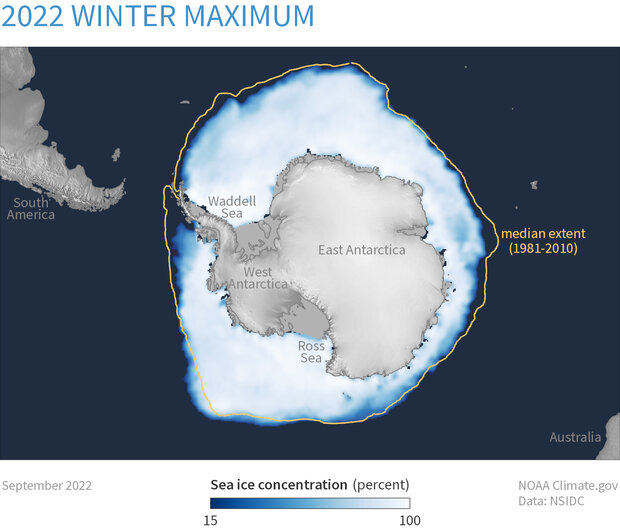
\includegraphics[width=\linewidth]{Figures/LiteratureReview/AntarcticClimate/seaIceExtentWinter2022.png} 
 		%\caption{Original Image}
	\end{subfigure}
	\hfill
	\begin{subfigure}[t]{.48\linewidth}
        \centering
		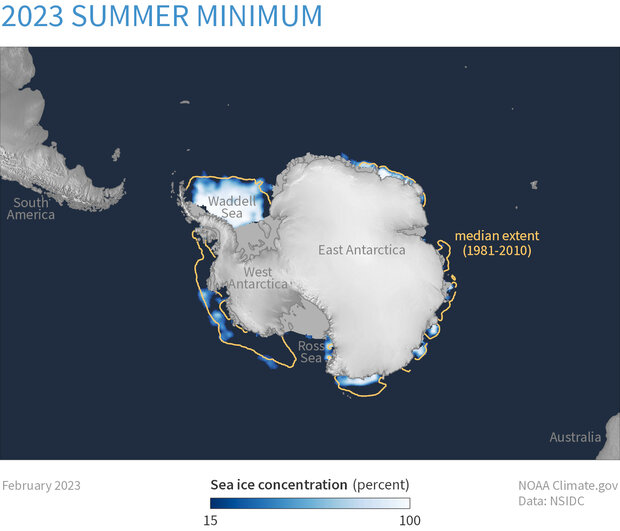
\includegraphics[width=\linewidth]{Figures/LiteratureReview/AntarcticClimate/seaIceExtentSummer2023.png} 
 		%\caption{Rotated Image \label{fig:dataRotate}}
	\end{subfigure}
    \caption{Comparison of sea ice extent in Antarctica between the winter of 2022 and summer of 2023. Taken from \cite{Scott2023}}
    \label{fig:litReview.antarcticClimate.seaIceExtent2022}
\end{figure}

%The maximum and minimum of this sea ice extent can vary year-on-year, and over the past 35 years, Antarctic sea ice extent has been observed to have slightly increased over each decade \cite{Comiso2017,Maksym2012,Simmonds2015}. This observation disagrees with the predictive models applied to model the Antarctic sea ice extent. Simmons investigated the application of \ac{cmip5}\footnote{\acs{cmip5}, which forms part of the \ac{cmip}, serves as a standard experimental framework designed to examine the output of coupled atmosphere-ocean general circulation models. This approach allows for the evaluation of a climate model's strengths and weaknesses when analysing climate variability and change. An overview of \acs{cmip5} can be found in the following paper by Taylor \cite{Taylor2012}.} models in Antarctica \cite{Simmonds2015} and discovered that these models perform well when analysing sea ice extent over 35 years in the Arctic \cite{Simmonds2015}, however, applying these models to Antarctica results in a decrease in sea ice extent being predicted. This is in direct opposition to the observations made in \cite{Comiso2017,Maksym2012}.


The maximum and minimum extents of sea ice can vary from year to year. Over the past 35 years,  a slight increase in Antarctic sea ice extent each decade has been observed \cite{Comiso2017,Maksym2012,Simmonds2015}. However, these observations contrast with predictive models used to estimate the Antarctic sea ice extent. Simmons \cite{Simmonds2015} examined the application of \ac{cmip5}\footnote{\acs{cmip5}, which forms part of the \ac{cmip}, serves as a standard experimental framework designed to examine the output of coupled atmosphere-ocean general circulation models. This approach allows for the evaluation of a climate model's strengths and weaknesses when analysing climate variability and change. An overview of \acs{cmip5} can be found in the following paper by Taylor \cite{Taylor2012}.} models in Antarctica. Simmons found that these models perform well in analysing Arctic sea ice extent over a 35-year period. However, when applied to Antarctica, these models predict a decrease in sea ice extent, contrary to the observations made in \cite{Comiso2017,Maksym2012}.

%Simmonds suggests that the discrepancies between the model outputs of the Arctic and the Antarctic can be attributed to natural variability \cite{Simmonds2015}. Simmonds also argues that, due to the period of study (35 years), the natural variability is less of an issue to the incorrect simulation outputs. Simmonds rather suggests that the differences can be attributed to the physics of the models; due to the fact that the \acs{cmip5} models work well when simulating Arctic ice, but poorly for Antarctic sea ice \cite{Simmonds2015}. This idea is confirmed by Maksym et al. due to the fact that pancake ice is not yet included in these types of models \cite{Maksym2012}. Pancake ice is an important part of the \acs{miz}, as well as a key process in sea ice-ocean interactions, and is discussed in the following sub-sections.

Simmonds suggests that the discrepancies between the model outputs of the Arctic and the Antarctic can be attributed to natural variability \cite{Simmonds2015}. He also argues that, given the 35-year study period, natural variability has less impact on the incorrect simulation outputs. Instead, Simmonds proposes that the differences can be attributed to the physics of the models. This is supported by the fact that the \acs{cmip5} models perform well in simulating Arctic ice but poorly in simulating Antarctic sea ice \cite{Simmonds2015}. This idea confirms the work of Maksym et al. \cite{Maksym2012}, as pancake ice, a significant component of the \acs{miz} and a key factor in sea ice-ocean interactions, is not yet considered in these models. The importance of pancake ice is discussed in the following sub-sections.

%Maksym et al. build on this idea that the physics of the sea ice models used in the Arctic will not translate to the Antarctic by introducing the differences between the two polar regions. The main differences can be attributed to the geography, sea-ice growth and decay, climate interactions, and ice-ocean interactions \cite{Maksym2012}. In terms of geography, the sea ice in the Arctic is landlocked by the Eurasian and North American continents \cite{Maksym2012,Parkinson2004} and is much more protected than sea ice in Antarctica, which is exposed to the \acs{so}. This means that sea ice in the Arctic is perennial\footnote{Perennial ice refers to ice packs that last more than one year and do not melt during the summer months}, whereas sea ice in the Antarctic is seasonal. As previously mentioned, the range of the sea ice extent in Antarctica is 1.5 times the extent of the Arctic \cite{Thomas2017}. In terms of climate interactions, the \acs{so} has extremely strong westerly winds, which results in large waves and frequent storms \cite{Maksym2012}. These westerly winds have caused the sea ice to extend further north\footnote{This is due to the fact that ice drifts to the left of the westerly winds due to a mechanism known as Ekman transport \cite{Maksym2012}} and increases the sea ice extent, which exposes sea ice to warmer temperatures \cite{Parkinson2004,Maksym2012}. The roughness and vastness of the \acs{so} are responsible for the difference in ice-ocean interactions between Arctic and Antarctic sea ice \cite{Parkinson2004} and is a dynamic system that is constantly in motion \cite{Maksym2012}. These mechanisms are discussed further in the following sub-sections, as well as the theory chapter.

Maksym et al. \cite{Maksym2012} build upon the idea that the physics of sea ice models used in the Arctic may not be directly applicable to the Antarctic. They introduce the distinctions between these two polar regions, highlighting key differences. The main disparities can be attributed to geographical factors, sea ice growth and decay patterns, climate interactions, and ice-ocean dynamics. In terms of geography, Arctic sea ice is enclosed by the Eurasian and North American continents \cite{Maksym2012, Parkinson2004}, affording it greater protection compared to the more exposed Antarctic sea ice, which interacts with the \acs{so}. Consequently, Arctic sea ice is considered perennial\footnote{Perennial ice refers to ice packs that persist for more than one year and do not melt during the summer months}, whereas Antarctic sea ice is seasonal. As mentioned earlier, the extent of sea ice in Antarctica is 1.5 times greater than that of the Arctic \cite{Thomas2017Chap8}. Regarding climate interactions, the \acs{so} experiences strong westerly winds, resulting in substantial waves and frequent storms \cite{Maksym2012}. These prevailing westerly winds drive the sea ice northward\footnote{This is due to the ice being pushed to the left of the westerly winds through a mechanism known as Ekman transport \cite{Maksym2012}}, expanding the sea ice coverage and consequently exposing it to warmer temperatures \cite{Parkinson2004, Maksym2012}. The roughness and vastness of the \acs{so} account for the distinctions in ice-ocean interactions between Arctic and Antarctic sea ice \cite{Parkinson2004}, which constitutes a dynamic system characterised by constant motion \cite{Maksym2012}.

%From the above literature, it can be seen that a large scientific effort is required to create accurate predictive models of Antarctica, rather than trying to apply predictive models built for an Arctic environment. The harshness of the Antarctic climate has meant that, particularly during winter, field measurements of the spatial distribution of sea ice in Antarctica are lacking \cite{Maksym2012}. Gherardi et al., and Kennicut et al. both agree that improved remote sensing techniques need to be implemented to monitor the extent of sea ice in Antarctica \cite{Gherardi2015,Kennicut2019}. Maksym et al. go one step further, by hypothesising that the thickness of sea ice may be more sensitive to climate variability than extent \cite{Maksym2012}, which explains the increase in melt, but also the increase in extent discussed. However, in-situ measurements are required to measure ice thickness in Antarctica instead of remote sensing techniques - as employed in the Arctic \cite{Gherardi2015,Thomas2017}. Maksym et al. argue that if researchers lack the ability to evaluate models of Antarctic sea ice, the confidence in the accuracy of projections will be brought into question, as models cannot capture the current state of sea ice in Antarctica \cite{Maksym2012}. This shows the need for the development of a pipeline to extract sea ice parameters in Antarctica, however, the issues discussed above cannot be mitigated. The differences between Arctic and Antarctic models are the presence of the \acs{miz} and pancake ice in this region, which is a key process in the sea ice-ocean interactions \cite{Maksym2012}. 

From the literature above, it is evident that significant scientific endeavour is necessary to create accurate predictive models of Antarctic sea ice, rather than attempting to apply predictive models built for an Arctic environment. The severity of the Antarctic climate has resulted in a lack of field measurements, particularly during winter, regarding the spatial distribution of sea ice in Antarctica \cite{Maksym2012}. Both Gherardi et al. \cite{Gherardi2015} and Kennicut et al. \cite{Kennicut2019} agree that implementing improved remote sensing techniques is essential to monitor the extent of sea ice in Antarctica. Taking this further, Maksym et al. \cite{Maksym2012} hypothesise that the thickness of sea ice may be more responsive to climate variability than sea ice extent. This not only explains the increase in melt but also the discussed increase in extent. However, measuring ice thickness in Antarctica requires in-situ measurements instead of the remote sensing techniques employed in the Arctic \cite{Gherardi2015, Thomas2017Chap8}.

Maksym et al. \cite{Maksym2012} argue that the inability to evaluate models of Antarctic sea ice by researchers raises questions about the accuracy of projections. This is because models fail to capture the current state of sea ice in Antarctica. This highlights the necessity for developing a pipeline to extract sea ice parameters in Antarctica. Nonetheless, the aforementioned issues cannot be easily mitigated. Notably, the differences between Arctic and Antarctic models include the interactions between the \acs{miz} and the \acs{so}, and pancake ice, which play a crucial role in sea ice-ocean interactions in Antarctica.


\subsection{Marginal Ice Zone} \label{subsec:litReview.antarctica.miz}
% Explain ice-ocean interaction (Link to theory section - only provide overview!)
% Chapter 8 of Sea-Ice
%The \ac{miz} in Antarctica is defined as the area that is close enough to the \ac{so} to be affected by its presence \cite{Wadhams1986}. The \ac{miz} in Antarctica is a dynamic system due to the prevalence of strong westerly winds and storms in the ice-free zones of the \acs{so} \cite{Massom2010, Brouwer2022, Maksym2012}, allowing for greater freedom of movement. The \acs{miz} is a region where sea-ice-ocean-atmosphere interactions are closely linked \cite{Wadhams1986, Vichi2019}. As discussed, the climate of Antarctica and the \acs{so} is incredibly harsh. The sea ice in the Antarctic \acs{miz} plays an important role in the interconnected global climate and being able to understand \acs{miz} dynamics allows the response of Antarctic sea ice, as well as the impacts of this, to climate change and variability to be understood \cite{Brouwer2022}. The \acs{miz} is controlled by a variety of processes, which are introduced in the following sub-section and discussed in more detail in the theoretical development chapter.

The \ac{miz} in Antarctica is defined as the area that is close enough to the \ac{so} to be affected by its presence \cite{Wadhams1986}. This region experiences dynamic conditions due to the prevalence of strong westerly winds and storms in the ice-free zones of the \acs{so} \cite{Massom2010, Brouwer2022, Maksym2012}, allowing for greater freedom of movement. The \acs{miz} is a region where sea-ice-ocean-atmosphere interactions are closely linked \cite{Wadhams1986, Vichi2019}. As discussed, the climate of Antarctica and the \acs{so} is incredibly harsh. Sea ice within the Antarctic \acs{miz} plays a crucial role in the global climate system \cite{Parkinson2004}, and comprehending the dynamics of the MIZ contributes to understanding the responses of Antarctic sea ice to climate change and variability, along with its associated impacts \cite{Brouwer2022}. The \acs{miz} is influenced by a variety of processes, which will be introduced in the following subsection.

The \acs{miz} plays a critical role in the global climate by forming a seasonal, insulating "skin" atop the \acs{so}. Due to the characteristics of sea ice, its high albedo reflects solar radiation and serves as an effective insulator \cite{Parkinson2004, Massom2010}. Consequently, sea ice within the \acs{miz} helps regulate \acs{so} temperatures by limiting heat exchanges between the \acs{so} and the atmosphere \cite{Parkinson2004}. Moreover, the presence of sea ice over the \acs{so} increases the salinity and density of the \acs{so} due to the seasonal formation of sea ice \cite{Massom2010, Parkinson2004}. This aspect is crucial for global ocean circulation \cite{Thomas2017Chap8}. The increased density beneath the sea ice in the \acs{miz} leads to overturning and the formation of bottom water\footnote{The resulting \ac{aabw} is the coldest in the world and has far-reaching climatic impacts. More information on bottom water formation, as well as its importance to the global climate, can be found in \cite{Gordon2001,Thomas2017Chap8,Jacobs2004}.} \cite{Parkinson2004}.

%Further to the sea ice-atmosphere and ocean interactions discussed, the most important aspect of the \acs{miz}, in the context of this project, is the way in which the Antarctic \acs{miz} interacts with wave motion from the \acs{so} as well as the features of the \acs{miz} which regulate this process. Brouwer et al. summarise this process nicely, by saying that the wave-ice interactions are mutual. Brouwer et al. state that the waves, which propagate through the \acs{miz}, alter the properties of the sea ice, however, when doing so, the wave amplitude is attenuated through the energy required to alter the sea ice properties \cite{Brouwer2022}. The way in which sea ice in the \acs{miz} attenuates waves is similar to that of a low-pass filter \cite{Brouwer2022}. This means that waves with a higher frequency are attenuated - where the rate depends on the physical characteristics of the sea ice, such as floe size, thickness and concentration \cite{Squire2020,Montiel2022}.

In addition to the discussions on sea ice-atmosphere and ocean interactions, the most crucial aspect of the \acs{miz} in the context of this project is its interaction with wave motion from the \acs{so}, as well as the characteristics of the \acs{miz} that regulate this process. Brouwer et al. \cite{Brouwer2022} summarise this phenomenon by stating that wave-ice interactions are mutual. According to Brouwer et al., the waves propagating through the \acs{miz} modify the properties of the sea ice. However, during this process, the wave amplitude is attenuated due to the energy required to alter the sea ice properties. The manner in which sea ice within the \acs{miz} attenuates waves is comparable to that of a low-pass filter. This implies that waves with higher frequencies are attenuated, with the rate of attenuation depending on the physical characteristics of the sea ice, such as floe size, thickness, and concentration \cite{Squire2020, Montiel2022}.

%Stammerjohn et al. state that these sea ice-ocean interactions are important to understand as they impact the sea ice features and distribution, which, in turn, impacts the regional, polar climate and global climate \cite{Stammerjohn2012}. This impact has been observed by Asplin et al. and Stopa et al., albeit in the Arctic \acs{miz}, whereby surface gravity waves, with a long period\footnote{The dynamics of ocean waves, as well as the different types for shallow and deep water, are explained quantitatively in the theoretical development section of this report. For the readers' interest, more information can be found in \cite{Holthuijsen2007}.}, have penetrated hundreds of kilometres into the Arctic \acs{miz} before being completely attenuated \cite{Asplin2012,Stopa2018}. This is an important observation, even for the Antarctic \acs{miz}, as long-period and high-amplitude waves occur frequently due to the harshness of the \acs{so} \cite{Young2020}, and the way in which these waves penetrate and become attenuated in the Antarctic \acs{miz} needs to be understood \cite{Alberello2021,Weeks2011}.

Stammerjohn et al. \cite{Stammerjohn2012} state that understanding sea ice-ocean interactions is crucial, as they influence sea ice features and distribution. These, in turn, affect both regional and polar climates, as well as the global climate. This impact has been observed in the Arctic \acs{miz} by Asplin et al. \cite{Asplin2012} and Stopa et al. \cite{Stopa2018} These researchers noted the penetration of long-period surface gravity waves\footnote{For an in-depth, quantitative explanation of ocean wave dynamics, including various types in shallow and deep waters, refer to the theoretical development section in this report. Additional information can be found in \cite{Holthuijsen2007}.}, reaching hundreds of kilometres into the Arctic \acs{miz} before being completely attenuated \cite{Asplin2012,Stopa2018}. This observation holds significance not only for the Arctic but also for the Antarctic \acs{miz}, where long-period and high-amplitude waves occur frequently due to the harshness of the \acs{so} \cite{Young2020}. It is imperative to understand how these waves penetrate and are attenuated within the Antarctic \acs{miz} \cite{Alberello2021}.

%This understanding is required because currently the \acs{miz} is viewed using remote sensing techniques via passive satellite technology to define the \acs{miz} using \ac{sic}. The ice edge is defined as 15\,\% \acs{sic}, whereas close ice is defined as 80\,\% \acs{sic} \cite{WMO2014}. However, using this metric to define the \acs{miz}, is not ideal, as it does not take into account wave interactions with the sea ice \cite{Brouwer2022}. According to Vichi, the use of \acs{sic} to understand the \acs{miz} characteristics in the Arctic is effective, however, applying this to the Antarctic \acs{miz} is not as reliable \cite{Vichi2021}. Vichi states that this is due to increased wave penetration and sea ice drift \cite{Vichi2019,Vichi2021}. Instead of using \acs{sic}, Vichi proposes a different approach to defining the \acs{miz}. Vichi's proposal is one that uses the statistical properties of \acs{sic} in the \acs{miz}, as well as the spatial and temporal variability of the \acs{sic} in the \acs{miz} \cite{Vichi2021}. This will allow the effects of different ice types, as well as wave action from the \acs{so} to be considered. 

This understanding is required because the current definition of the \acs{miz} relies on remote sensing techniques employing passive satellite technology to define the \acs{miz} through the use of \ac{sic}. The ice edge is conventionally defined as having 15\,\% \acs{sic}, while compact ice is characterized by 80\,\% \acs{sic} \cite{WMO2014}. However, employing this metric to define the Antarctic \acs{miz} is inefficient, as it overlooks wave interactions with the sea ice \cite{Brouwer2022,Vichi2021}. According to Vichi \cite{Vichi2021}, the use of \acs{sic} to comprehend \acs{miz} characteristics in the Arctic is effective; whilst, its application to the Antarctic \acs{miz} lacks reliability. Vichi \cite{Vichi2019,Vichi2021} asserts that this discrepancy is attributed to heightened wave penetration and sea ice drift. In place of \acs{sic}, Vichi proposes an alternate approach to defining the \acs{miz}. Vichi's recommendation involves utilising the statistical properties of \acs{sic} within the \acs{miz}, alongside the spatial and temporal variability of \acs{sic} in the same zone \cite{Vichi2021}. This approach will enable the consideration of distinct ice types, along with wave activity from the \acs{so} \cite{Vichi2021}.


\subsection{Pancake Ice} \label{subsec:litReview.antarctica.pancakeIce}
% Importance of pancake ice
% Mention frazil ice
% WHY pancake ice forms in the Antarctic and is important in it
% Yearly life cycle of pancake ice

As noted by Maksym et al. \cite{Maksym2012}, one of the key processes in the Antarctic \acs{miz} is pancake ice formation. Given the vastness of the \acs{so} and the prevalence of the \acs{miz} in Antarctica, the existence of waves within the \ac{miz} significantly influences the types of ice found within the \acs{miz} \cite{Brouwer2022}. This section provides a brief introduction to the formation and life cycle of pancake ice, followed by an exploration of its significance in shaping the Antarctic climate. Furthermore, this section introduces its crucial role in Antarctic sea ice modelling.

The formation of pancake ice in the \acs{miz} is poorly understood \cite{Doble2003}. In summer, large ice floes make up the \acs{miz}, whereas, in winter the \acs{miz} is made up of millions of smaller pancake ice floes \cite{Alberello2019,Alberello2021b} The presence of the rough sea surface means that the formation of ice is not allowed to settle into a fully formed ice sheet. Rather, when sea ice begins to form in the Antarctic in winter, it begins to create a suspension of crystals known as frazil ice \cite{Doble2003,Wadhams1999}. Over time, these frazil crystals converge, due to roughened seas, and collect to form small cakes \cite{Doble2003,Dierking2013} Initially, these small cakes are referred to as "dollar pancakes" \cite{Wadhams1999}, with a diameter of approximately 2-3\,cm and a thickness of only a few millimetres \cite{Doble2003,Wadhams1999}. At greater distances from the ice edge in the \acs{miz}, these dollar pancakes can fuse together due to wave attenuation, forming larger pancakes with a diameter of up to 5\,m and a thickness of approximately 50\,cm \cite{Wadhams1999,Aulicino2014,Doble2003}. In 2019, Alberello et al. \cite{Alberello2019} found that approximately 50\,\% of the observed sea ice area was made up of pancake ice floes ranging from 2.3 - 4m in diameter. Only further into the \acs{miz}, at approximately 270\,km \cite{Wadhams1987}, where wave action has been attenuated even more, can these pancakes freeze together to form an ice sheet known as consolidated pancake ice. Once consolidated pancake ice is formed, thickening of these consolidated pancakes occurs to form pack ice \cite{Doble2003}. 

% How it influences climate - why the ice plays a vital role 

%Pancake ice formation is key to pack ice formation in Antarctica \cite{Clarke1984,Lange1991} and as discussed in Section \ref{subsec:litReview.antarctica.miz}, the importance of sea ice is critical to the global climate and understanding the processes behind the formation, evolution and distribution of sea ice, particularly pancake ice, is vital to explain the geophysical interactions in the polar regions, particularly the \acs{miz} \cite{DeCarolis2002}. Firstly, pancake ice is important in the production of a fertile winter ecosystem due to its ability for increased algal growth and shelter for krill due to its rafted bottom which provides a large surface area \cite{Wadhams2002}. Secondly, the gravity-induced drainage of brine after pancake formation is responsible for regulating the salinity of the \acs{so}, as well as previously discussed, the high albedo of sea ice provides an insulating layer on top of the \acs{so}, and helps in regulating \acs{so} temperatures \cite{Doble2003}.

Pancake ice formation is key to pack ice formation in Antarctica \cite{Clarke1984,Lange1991}. As discussed in Section \ref{subsec:litReview.antarctica.miz}, the importance of sea ice is critical to the global climate. Understanding the processes behind the formation, evolution, and distribution of sea ice, particularly pancake ice, is vital for explaining the geophysical interactions in the polar regions, especially the \acs{miz} \cite{DeCarolis2002}.

Firstly, pancake ice plays a significant role in the production of a fertile winter ecosystem due to its ability to promote increased algal growth and provide a shelter for krill. Its rafted bottom creates a large surface area \cite{Wadhams2002}. Secondly, the gravity-induced drainage of brine after pancake formation helps regulate the salinity of the \acs{so}. Additionally, as previously discussed, the high albedo of sea ice serves as an insulating layer atop the \acs{so} and aids in regulating its temperatures \cite{Doble2003}.

%The modelling of pancake ice is not particularly well understood and is currently being incorporated into existing sea ice models \cite{Alberello2019}. The understanding of pancake ice, particularly its impact on wave attenuation is important as according to both Doble et al. and Alberello et al. \cite{Alberello2019,Doble2015}, increased open water area present in the Arctic is causing an increased presence of pancake ice in the region. This is important, as the models which currently exist for this region, are slowly becoming less accurate due to these changes in the region's sea ice composition \cite{Doble2015}.

The modelling of pancake ice is not particularly well understood and is currently being incorporated into existing sea ice models \cite{Alberello2019}. The understanding of pancake ice, particularly its impact on wave attenuation, is important, as indicated by both Doble et al. \cite{Doble2015} and Alberello et al. \cite{Alberello2019}. The increased open water area in the Arctic is leading to a greater presence of pancake ice in the region \cite{Alberello2019,Doble2015}. This is significant because the existing models for this region are gradually decreasing in accuracy due to the changing composition of the sea ice in the region. In order to properly model the region, sea ice models including properly characterised pancake ice floes are required \cite{Doble2015}.


%====================================================
\section{Characterisation of Sea Ice}
\label{sec:litReview.seaIceCharac}
% Existing technology and work (not necessarily SAR)
% Chapter 9 of Sea-Ice
% Importance of ocean waves in modelling (Holthuijsen)

This section will introduce the existing technologies and research that have been employed to characterise sea ice in both the Arctic and Antarctic regions. These methods will be briefly examined, focusing on their advantages and disadvantages in implementation. Subsequently, the technique of sea ice characterisation using \acs{sar} will be introduced in the subsequent section. The importance of ocean waves in modelling will also be discussed. As mentioned earlier, the differentiation between Arctic and Antarctic sea ice modelling will be emphasised in relation to these technologies.

While in-situ measurements are the most practical method for determining sea ice characteristics, as discussed in Section \ref{sec:litReview.antarcticClimate}, a vast expanse of the Antarctic \acs{miz} is inaccessible in winter due to the formation of thick sea ice that cannot be navigated, even by ice-breaking ships \cite{Maksym2012}. Thus, remote sensing techniques\footnote{Spreen and Kern \cite{Thomas2017Chap9} define remote sensing as any form of data acquisition without the need for physical contact or measurement.} need to be implemented to monitor the Antarctic \acs{miz} year-round due to the harshness of the region \cite{Kennicut2019, Maksym2012}. Since the scope of this project revolves around \acs{sar} - a remote sensing technique in itself - this section will focus on remote sensing techniques for sea ice characterisation.

Remote sensing techniques rely on the \ac{em} spectrum and satellite remote sensing of sea ice is conducted in multiple parts of the \acs{em} spectrum \cite{Thomas2017Chap9}. Different frequency ranges of the spectrum are used, and the reflected intensity measured by the sensors depends on the ability of sea ice, water, and snow to emit \acs{em} radiation. The ability of sea ice to emit this \acs{em} radiation is determined by its geophysical properties, such as salinity, roughness, and air content \cite{Thomas2017Chap9}. These geophysical properties can be inferred from the received intensity at the sensor. The \acs{em} radiation emitted back by sea ice can originate from either a passive source, such as the sun, or an active source, such as a \acs{sar} transmitter. The following sub-sections introduce three different remote sensing techniques which operate at different frequencies in the \acs{em} spectrum.

\subsection{Microwave radiometry and scatterometry} \label{subsec:litReview.seaIceCharac.radiometry}

For optimal sea ice microwave remote sensing, frequencies of less than 10\,GHz are used. While higher frequencies result in better spatial resolution, the influence of atmospheric conditions increases. Thus, microwave remote sensing of sea ice always involves a trade-off between atmospheric influence and spatial resolution \cite{Thomas2017Chap9}.

Microwave radiometry has been employed to measure sea ice extent and types. For sea ice extent determination, both microwave radiometry and scatterometry have been utilised. To gauge sea ice extent through microwave radiometry, the brightness temperature, denoted as $T_{B}$, plays a significant role. $T_{B}$ is predominantly influenced by the emissivity\footnote{Emissivity, a material-specific property, is a function of the dielectric properties of the material \cite{Thomas2017Chap9}.} of the sea ice or sea surface. The distinction in $T_{B}$ between the sea ice and sea is utilised to define the sea ice extent. However, this approach encounters limitations when the sea surface becomes roughened by wind, leading to an increase in the emissivity of the sea's surface. Consequently, the $T_{B}$ of the sea surface reaches a similar level to that of the sea ice \cite{Thomas2017Chap9}. In the context of Antarctica, this issue arises due to the rough nature of the \acs{so}, potentially interfering with the differentiation between sea ice and the ocean surface. 

Scatterometry can also be used to determine sea ice extent. The difference in radar backscatter\footnote{Backscatter is the reflection of a signal back towards its source} between uncovered open water and sea ice enables the detection of an ice-covered region \cite{Thomas2017Chap9}. Rivas et al. \cite{Rivas2018} discovered that scatterometry is more accurate than microwave radiometry in determining sea ice extent, especially when the edge of the extent is composed of frazil ice.

The backscatter of different ice types differs depending on the ice's salinity, density, roughness, temperature, and snow coverage \cite{Thomas2017Chap9}. This differentiation allows the identification of various types of ice within a sea ice region based on the received backscatter intensity. Dierking \cite{Dierking2001} found that pancake ice exhibits higher radar backscatter compared to other ice types due to its increased surface roughness and the presence of numerous edges. This observation has been confirmed by Lange and Eicken \cite{Lange1991} through their study of higher radar backscatter in the Antarctic \acs{miz}.

\subsection{Altimetry} \label{subsec:litReview.seaIceCharac.altimetry}

Altimeters measure the time taken by an \acs{em} signal to be transmitted, reflected off the Earth's surface, and received. From this, the distance can be calculated. Laser and radar altimeters can be used to measure sea ice thickness. However, instead of directly measuring the thickness, these altimeters measure the sea ice freeboard\footnote{Freeboard is defined by Ricker et al. \cite{Ricker2015} as the height of sea ice above the local sea level.}, and infer the thickness from the sea surface height. To extract the surface elevation, the satellite's position in space needs to be known with centimetre accuracy \cite{Thomas2017Chap9}.

To calculate sea ice thickness, both the freeboard and sea surface height need to be determined by the altimeter. One issue with sea surface height determination is the need to access uncovered ocean to act as a reference point \cite{Thomas2017Chap9}. In order to convert freeboard height to sea ice thickness, the density and snow depths need to be known. Ricker et al. \cite{Ricker2015} show that the origin of the return signal of the altimeter cannot always be known with certainty and state that snow cover is not negligible in determining distances due to the fact that the signals do not penetrate the snow completely, thus creating bias in measurements. Given that Antarctica experiences some of the highest snowfall rates in the world \cite{Maksym2012}, this method will be unable to be implemented without the aid of in-situ measurements of snow depth \cite{Ricker2015}. Spreen and Kern \cite{Thomas2017Chap9} explain that improved retrieval methods using altimeters need to be implemented to overcome this.

\subsection{Optical and Thermal infrared imaging} \label{subsec:litReview.seaIceCharac.opticalThermal}

Optical and thermal infrared imaging techniques rely on the fact that sea ice reflects solar radiation more than open, uncovered water \cite{Thomas2017Chap9}. Optical imagery has been used to measure \acs{sic} \cite{Emery1994} as well as thickness. Thermal imaging is useful, as sensors can measure the surface temperature, $T_{\text{surface}}$, of sea ice \cite{Thomas2017Chap9}.

The average sea ice albedo is greater than 0.6, compared to the low albedo of water, which is 0.07. Brandt et al. found that the albedo of ice increased with thickness \cite{Thomas2017Chap9,Brandt2005}, allowing these techniques to be used for measuring ice thickness. To measure the surface albedo using a satellite, a sensor capable of measuring surface reflectance needs to be employed \cite{Thomas2017Chap9}.

The main disadvantage of this technology is its limitations. Both optical and thermal imaging technologies require daylight as well as clear sky conditions to capture the desired data. Clouds pose a significant challenge for both of these technologies. In the optical spectrum, clouds exhibit similar reflectivity to sea ice, and the infrared temperatures of the surface of sea ice and clouds are also similar \cite{Thomas2017Chap9}. These issues imply that while this technology has been utilised for parameter extraction of sea ice, it can only be applied within a narrow time frame determined by environmental conditions, preventing year-round coverage of Antarctica.

%====================================================
\section{Sea Ice Characterisation using SAR} 
\label{sec:litReview.sarCharac}
% Explain BRIEFLY what sar is and why it is used for sea ice characterisation
% Introduce section (Which satellites, as well as a brief overview of the inversion technique and its path to where we are now)
% What characteristics are important to the SAR process e.g. thickness for radar penetration and snow coverage for reflection
%% - Discuss differences in reflectiveness of different elements

[I need to beef this out still - I want to use the following sources, \cite{Dierking2013,Zakhvatkina2019,Thomas2017Chap9} to introduce the process followed by the \acs{irea} and discuss which \acs{sar} characteristics have been found to be important to the parameter extraction process of pancake ice.]

The main disadvantage of the remote sensing methods mentioned above is the low spatial resolution. \acs{sar} overcomes this by using the motion of a satellite to synthetically increase the size of the antenna \cite{Thomas2017Chap9}. \acs{sar} has been used to determine sea ice type through differences in radar backscatter. 

\subsection{SAR Satellites}
\label{subsec:litReview.sarCharac.satellites}
% Discuss the satellite technology needed to implement sar - specifically for polar regions
% TerraSAR-X, Sentinel-1, CosmosSkyMet, and others
% Sentinel-1 TODO

Due to the nature of orbits around the planet\footnote{For an orbit to capture polar regions, it needs to have a 90\,$^{\circ}$ inclination orbit \cite{PolarOrbitNasa}}, only specific \acs{sar} satellites can effectively monitor the polar regions \cite{Thomas2017Chap9}. These commonly used satellites are outlined in Table \ref{tab:litReview.sarCharac.satellites.commonlyUsed}, along with key features of interest. The meaning and significance of these features will be expanded on and explained in the subsequent chapter.

\begin{table}[H]
\resizebox{\textwidth}{!}{%
\begin{tabular}{|l|c|c|c|c|c|c|c|c|}
\hline
\textbf{Name} & \textbf{\begin{tabular}[c]{@{}c@{}}Frequency\\ (GHz)\end{tabular}} & \textbf{\begin{tabular}[c]{@{}c@{}}Frequency\\ Band\end{tabular}} & \textbf{\begin{tabular}[c]{@{}c@{}}Resolution\\ (m)\end{tabular}} & \textbf{\begin{tabular}[c]{@{}c@{}}Swath\\ (km)\end{tabular}} & \textbf{\begin{tabular}[c]{@{}c@{}}Incidence Angle\\ ($^\circ$)\end{tabular}} & \textbf{\begin{tabular}[c]{@{}c@{}}Inclination\\ ($^\circ$)\end{tabular}} & \textbf{Operational} & \textbf{Polarisation} \\ \hline
\textbf{ERS-1} and \textbf{2} & 5.3 & C & 30 & 100 & 20-26 & 98.5 & 1991-2011 & VV \\ \hline
\textbf{Envisat ASAR} & 5.3 & C & 30-1000 & 100-400 & 15-45 & 98.5 & 2002-2012 & Dual-polarimetric\footnote{Explain dual polarimetric polarisation} \\ \hline
\textbf{Radarsat-1} and \textbf{2} & 5.3/5.4 & C & 3-100 & 18-500 & 10-60 & 98.6 & 1995- & \begin{tabular}[c]{@{}c@{}}HH (RS-1)\\ Full\footnote{Explain full polarisation} (RS-2)\end{tabular} \\ \hline
\textbf{Sentinel-1} & 5.4 & C & 5-100 & 80-400 & 19-47 & 98.2 & 2014- & Full \\ \hline
\textbf{TerraSAR-X} & 9.6 & X & 1-40 & 5-200 & 15-60 & 97.4 & 2007- & Full \\ \hline
\textbf{ALOS-1} and \textbf{2 PALSAR} & 1.3 & L & 3-100 & 20-350 & 8-70 & 98.7 (AL-1), 97.9 (AL-2) & \begin{tabular}[c]{@{}c@{}}2006-2011 (AL-1)\\ 2014- (AL-2)\end{tabular} & Full \\ \hline
\textbf{COSMO-SkyMed} & 9.6 & X & 1-100 & 10-100 & 16-51 & 97.9 & 2007- & Dual-polarimetric \\ \hline
\end{tabular}}
\caption{Commonly used \acs{sar} sensors for sea ice research and a comparison of their important features. Adapted from \cite{Thomas2017Chap9}.}
\label{tab:litReview.sarCharac.satellites.commonlyUsed}
\end{table}

As per the scope of this project, this project will be using data obtained from Sentinel-1 and TerraSAR-X for pipeline development and testing. As such, these satellites will be investigated further in this subsection.

\subsubsection{Sentinel-1} \label{sybsubsec:litReview.sarCharac.satellites.sentinel}

%Sentinel-1 is the first of a series of operational satellites launched by the \ac{esa} as part of the \ac{gmes} - a European initiative to meet the Earth Observation needs of the European Union \cite{Attema2009}. The Sentinel-1 is a constellation of two \acs{sar} satellites that include both the Sentinel-1A and Sentinel-1B satellites, which were launched on April 3, 2014, and April 25, 2016, respectively \cite{Geudtner2014,Potin2019}. Sentinel-1 is equipped with an active phased array antenna operating at C-Band frequency \cite{Geudtner2014}, capable of functioning in various modes\footnote{These modes include Interferometric Wide Swath, Extra Wide Swath, StripMap, and Wave. All of these modes, except Wave, operate in dual polarization. More information on the Sentinel-1 imaging modes can be found in Figure 1 and Table 1 of \cite{Geudtner2014}.}. Sentinel-1 is capable of providing data to support multiple applications, however, the main application of interest is the ability to monitor sea ice zones which cover the Arctic and the Antarctic \cite{Attema2009,Geudtner2014}, as well as the open-source data policy \cite{Potin2019}.

Sentinel-1 is the first in a series of operational satellites launched by the \ac{esa} as part of the \ac{gmes} program - an initiative aimed at meeting the Earth Observation needs of the European Union \cite{Attema2009}. The Sentinel-1 constellation comprises two \acs{sar} satellites: Sentinel-1A and Sentinel-1B. These satellites were launched on April 3, 2014, and April 25, 2016, respectively \cite{Geudtner2014, Potin2019}. Equipped with an active phased array antenna operating at C-Band frequency, Sentinel-1 is capable of operating in various modes\footnote{These modes include \acf{iw}, \acf{ew}, \acf{sm}, and Wave. All these modes, except Wave, operate in dual polarization. Further details on the Sentinel-1 imaging modes can be found in Figure 1 and Table 1 of \cite{Geudtner2014}.}. While Sentinel-1 serves multiple applications, its primary focus is on monitoring sea ice zones in the Arctic and Antarctic regions \cite{Attema2009, Geudtner2014}, in addition to operating on an open-source data policy \cite{Potin2019}.

This application is achieved through the orbit of Sentinel-1. Both \ac{s1a} and Sentinel-1B fly in the same orbital plane; however, they are phased by 180\,$^{\circ}$\footnote{This phased orbit of the constellation means that the satellites are on opposite sides of the Earth at any given time. More information can be found in \cite{Geudtner2014}.}. The mission is on a sun-synchronous orbit\footnote{Sun-synchronous orbits allow a satellite to cross the same latitude at the same solar time of day on each orbit \cite{Hulley2019}.} and has a 12-day orbit repeat cycle \cite{Torres2012}. To ensure a polar orbit, the satellites have an inclination angle of 98.2\,$^{\circ}$, as shown in Table \ref{tab:litReview.sarCharac.satellites.commonlyUsed}. The open-source policy of this mission is useful for this project, as Level 0, Level 1, and Level 2 data products\footnote{The differentiation between these data is discussed in the theoretical development chapter.} are available for download on the \href{https://scihub.copernicus.eu/dhus/#/home}{Sentinel Copernicus Open Hub} \cite{Potin2019}.

The global coverage of Sentinel-1 in\acf{iw} mode is depicted in Figure \ref{fig:litReview.sarCharac.satellites.sentinel.coverage}. The captures encompassing the Antarctic continent in Figure \ref{fig:litReview.sarCharac.satellites.sentinel.coverage} are of particular interest to this project. Garkusha and Hnatushenko \cite{Garkusha2020} utilised data from this region to compile a mosaic of the entire Antarctic coastline using Sentinel-1 \acs{sar} data. The coverage of the coastline is illustrated in Figure \ref{fig:litReview.sarCharac.satellites.sentinel.coverageCoast.sentinel}. To achieve complete coverage for the construction of this mosaic, Garkusha and Hnatushenko employed GRD data from 98 captures from Sentinel-1. This mosaic construction is illustrated in Figure \ref{fig:litReview.sarCharac.satellites.sentinel.coverageCoast.mosaic}.

\begin{figure}[H]
    \centering
    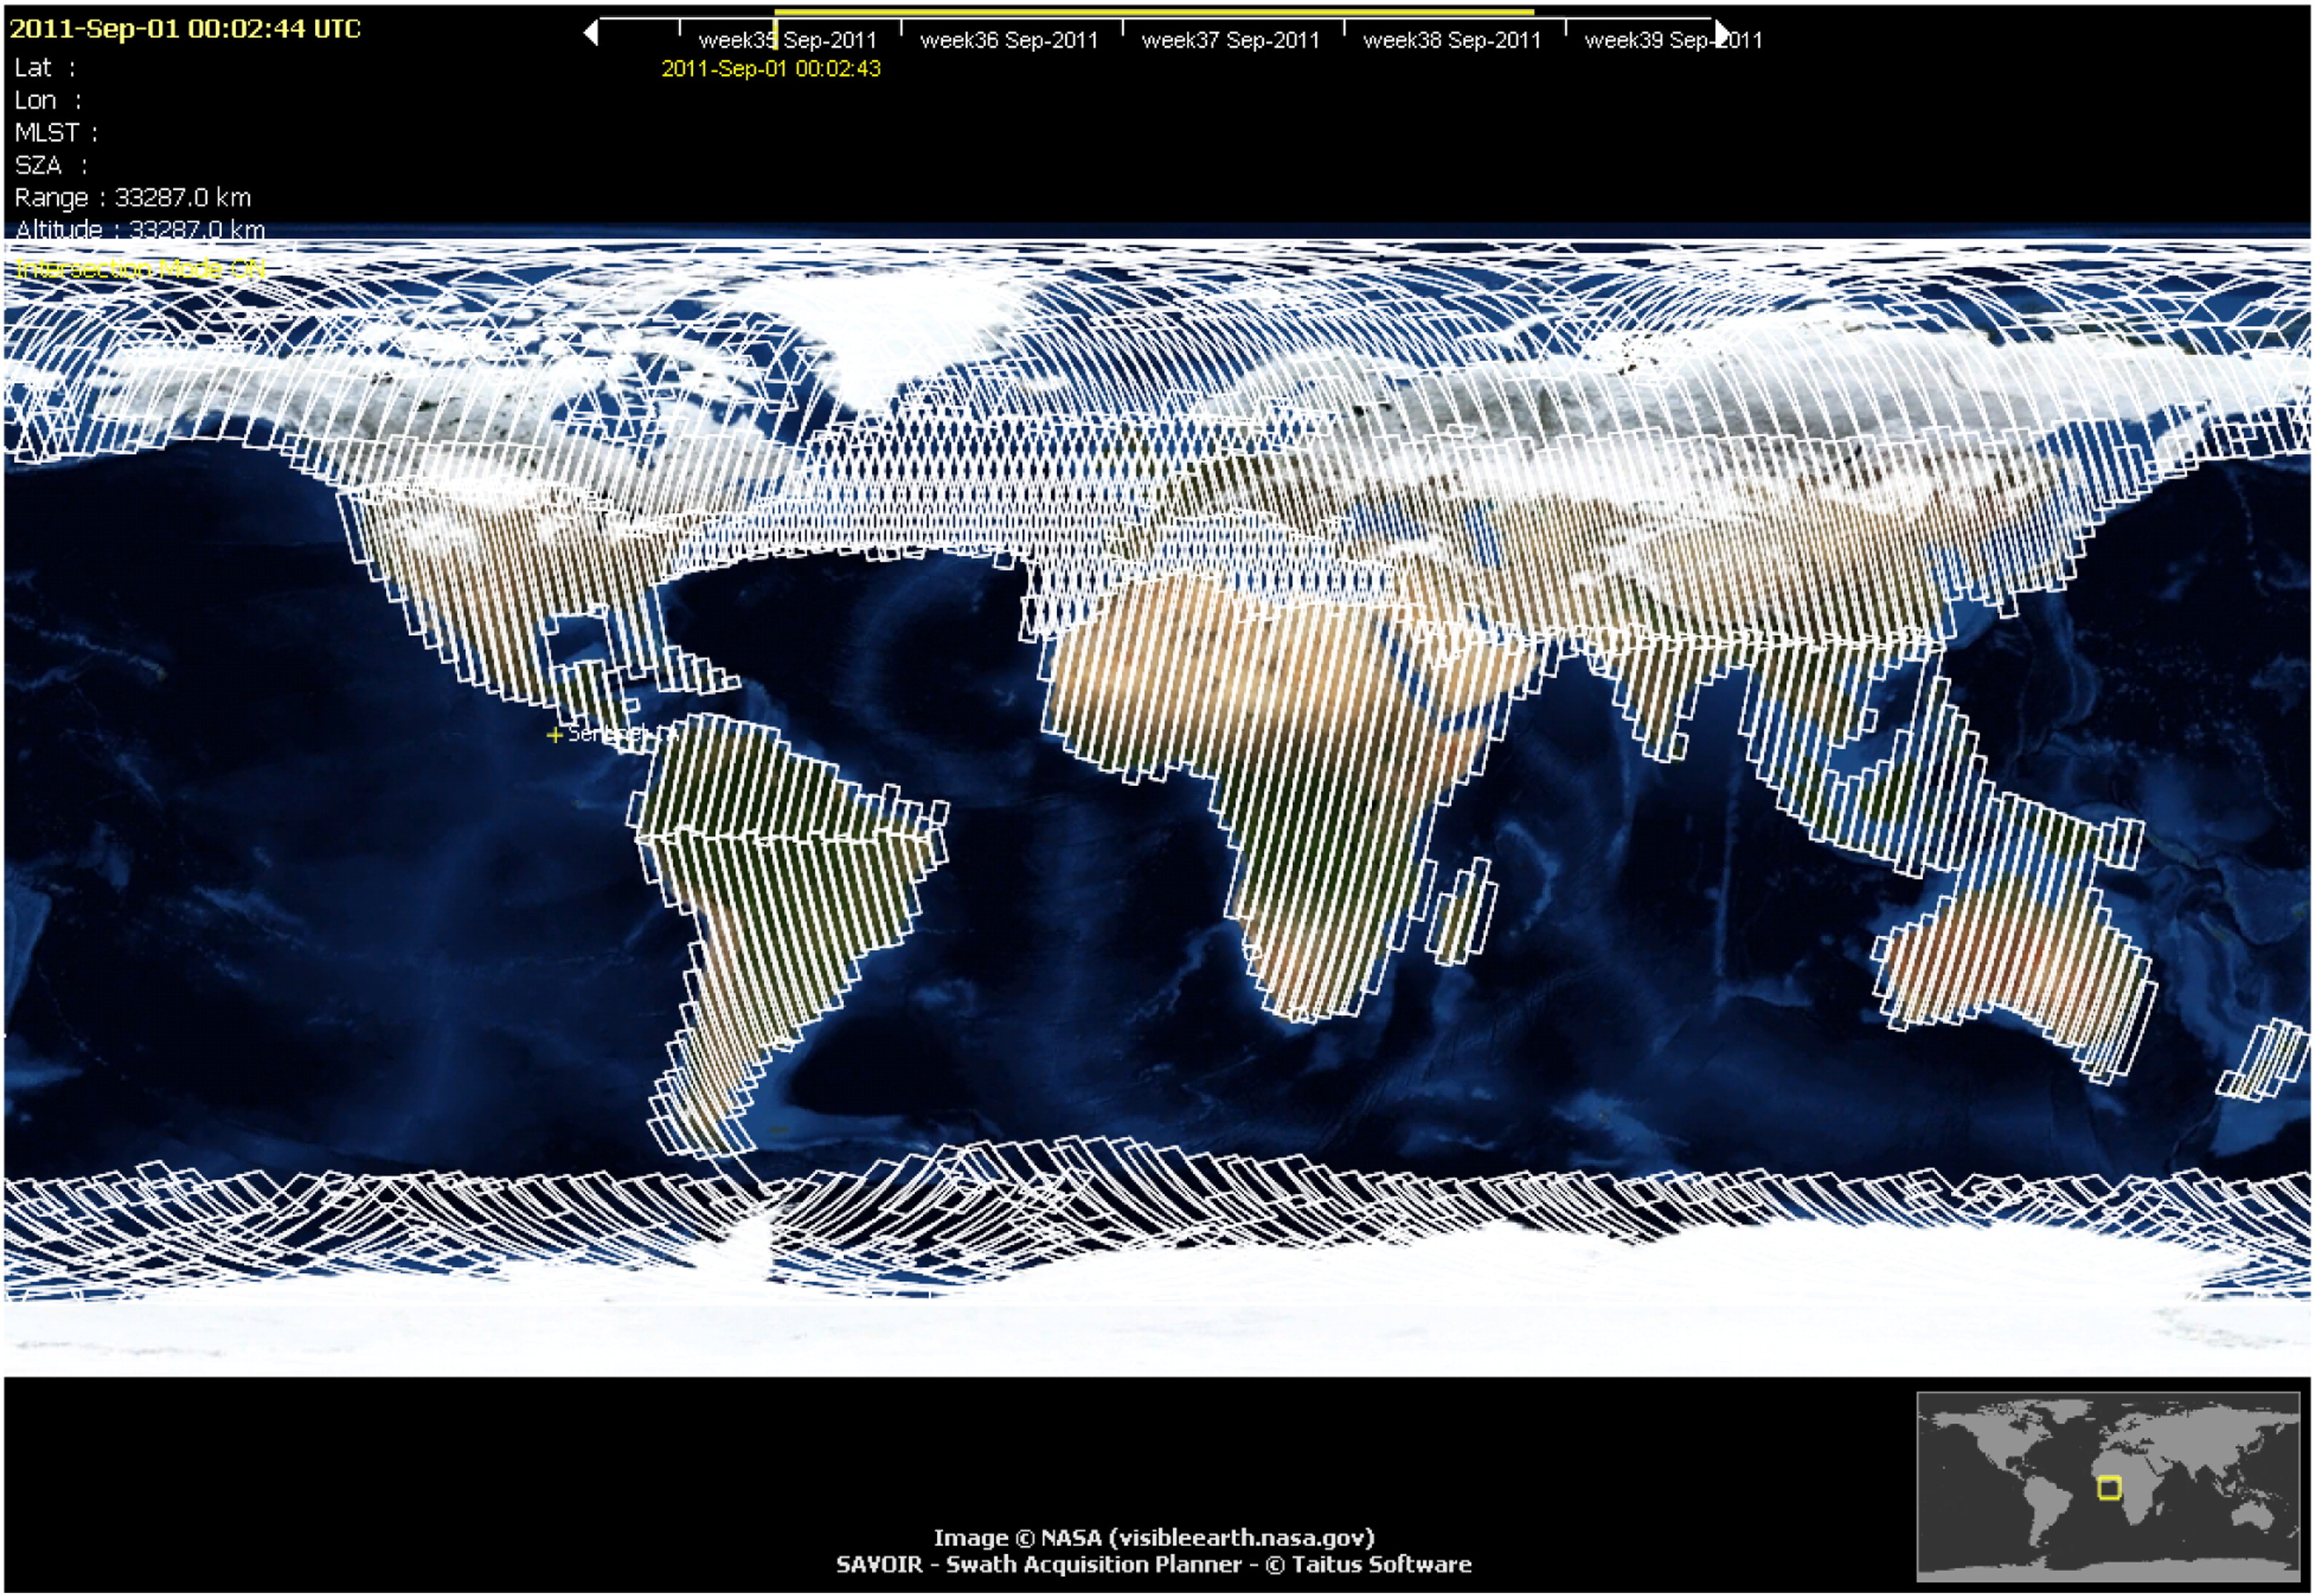
\includegraphics[width=.5\linewidth]{Figures/LiteratureReview/Satellites/sentinelCoverage.jpg}
    \caption{\ac{iw} mode coverage of one Sentinel-1 satellite after one 12-day orbit cycle. Taken from \cite{Torres2012b}.}
    \label{fig:litReview.sarCharac.satellites.sentinel.coverage}
\end{figure}

\begin{figure}[H]
	\centering
	\begin{subfigure}[t]{.48\linewidth}
		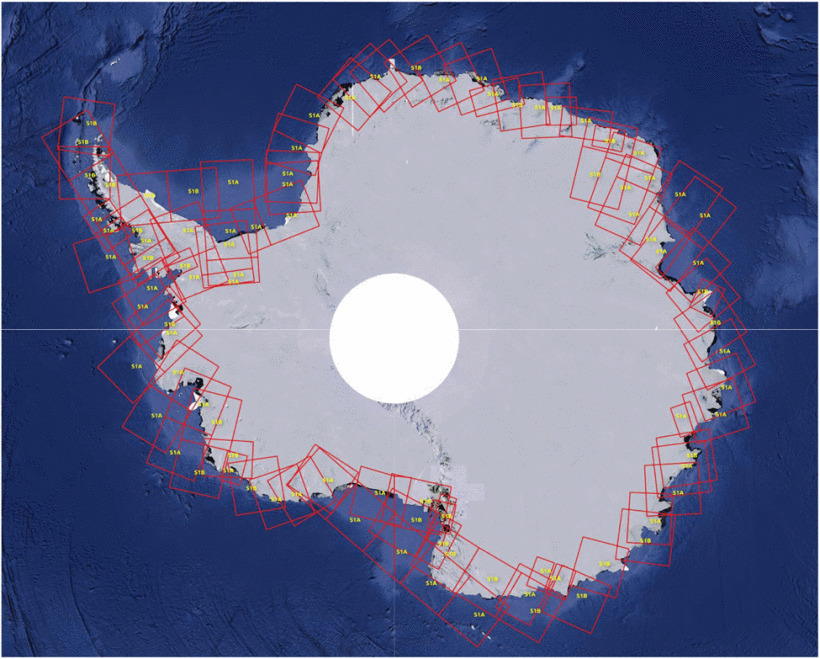
\includegraphics[width=\linewidth]{Figures/LiteratureReview/Satellites/sentinelCoverageCoast.jpg} 
 		\caption{Antarctic coastal coverage of Sentinel-1}
            \label{fig:litReview.sarCharac.satellites.sentinel.coverageCoast.sentinel}
	\end{subfigure}
	\hfill
	\begin{subfigure}[t]{.48\linewidth}
        \centering
		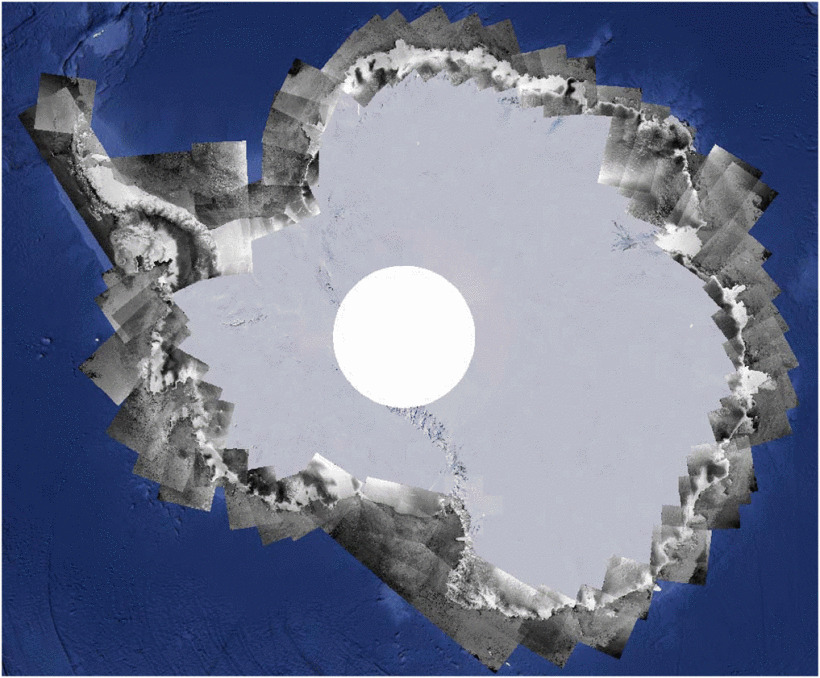
\includegraphics[width=0.98\linewidth]{Figures/LiteratureReview/Satellites/sentinelCoverageCoastMosaic.jpg} 
 		\caption{Constructed mosaic of the Antarctic coastline}
            \label{fig:litReview.sarCharac.satellites.sentinel.coverageCoast.mosaic}
	\end{subfigure}
    \caption{Antarctic coast line coverage and reconstructed continuous \acs{sar} image using Sentinel-1. Taken from \cite{Garkusha2020}.}
    \label{fig:litReview.sarCharac.satellites.sentinel.coverageCoast}
\end{figure}

Overall, the Sentinel-1 mission has been successful in capturing \acs{sar} data over Antarctica and the \acs{so}, as depicted in Figures \ref{fig:litReview.sarCharac.satellites.sentinel.coverage} and \ref{fig:litReview.sarCharac.satellites.sentinel.coverageCoast.sentinel}. Due to its open-source policy, the mission will be able to provide the desired data for this project.

\subsubsection{TerraSAR-X} \label{subsubsec:litReview.sarCharac.satellites.terraSAR}

The TerraSAR-X satellite is a German \acs{sar} satellite designed for scientific and commercial applications. It was launched on June 15, 2007 \cite{Werninghaus2004, Werninghaus2010}. TerraSAR-X continues the lineage of successful \acs{sar} missions initiated by \ac{nasa} and the \ac{asi}, notably X-SAR in 1994 and the \ac{srtm} in 2000, respectively \cite{Werninghaus2010}. The satellite is equipped with an active phased array antenna operating at X-Band frequency, capable of functioning in various modes\footnote{These modes include Spotlight, StripMap, and ScanSAR. Additional modes, Staring Spotlight and Wide ScanSAR, were introduced after enhancements in 2013, which enhanced azimuth resolution and extended swath width respectively \cite{Buckreuss2018}.}. Moreover, TerraSAR-X supports multiple polarisations. The mission has two objectives: firstly, to provide the scientific community with multi-mode X-Band \acs{sar} data, and secondly, to foster the development of a commercial Earth Observation market in Europe \cite{Werninghaus2004}.

In terms of instrumentation, the satellite is equipped with 12 panels, each containing 32 dual-polarised waveguide subarrays. The centre frequency is 9.65\,GHz, and the system has a bandwidth of 300\,MHz. The antenna can operate in both H and V polarisations.\footnote{The meaning of these parameters is not crucial in this section of the report. Their significance and meaning will be further elaborated on in the theoretical development chapter of this report}.\cite{Werninghaus2004} Further details about satellite instrumentation can be found in references \cite{Werninghaus2004, Werninghaus2010}.

The orbit of TerraSAR-X is of interest for remote sensing of Antarctica. The mission is on a sun-synchronous orbit\footnote{See footnote 16} and orbits the Earth 15 2/11 times per day and has a repeat orbit every 11 days, or every 167 orbits \cite{Pitz2010}. The inclination of the orbit is important to ensure that the polar regions are captured, and as seen in Table \ref{tab:litReview.sarCharac.satellites.commonlyUsed}, the inclination of TerraSAR-X is 97.4\,$^{\circ}$. 

Buckreuss et al. \cite{Buckreuss2018} conducted a 10-year review of TerraSAR-X in 2018 and, when focusing on the total number of data acquisition requests over this period, found that over 30,000 left-looking data acquisitions out of the 226,000 acquisitions had been made. Buckreuss et al. stated that this benefits the scientific community, as it meant StripMap acquisitions could be made over Antarctica. An image of these StripMap acquisitions over Antarctica is shown in Figure \ref{fig:litReview.sarCharac.satellites.terraSAR.antarcticStripmaps}.

\begin{figure}[H]
    \centering
    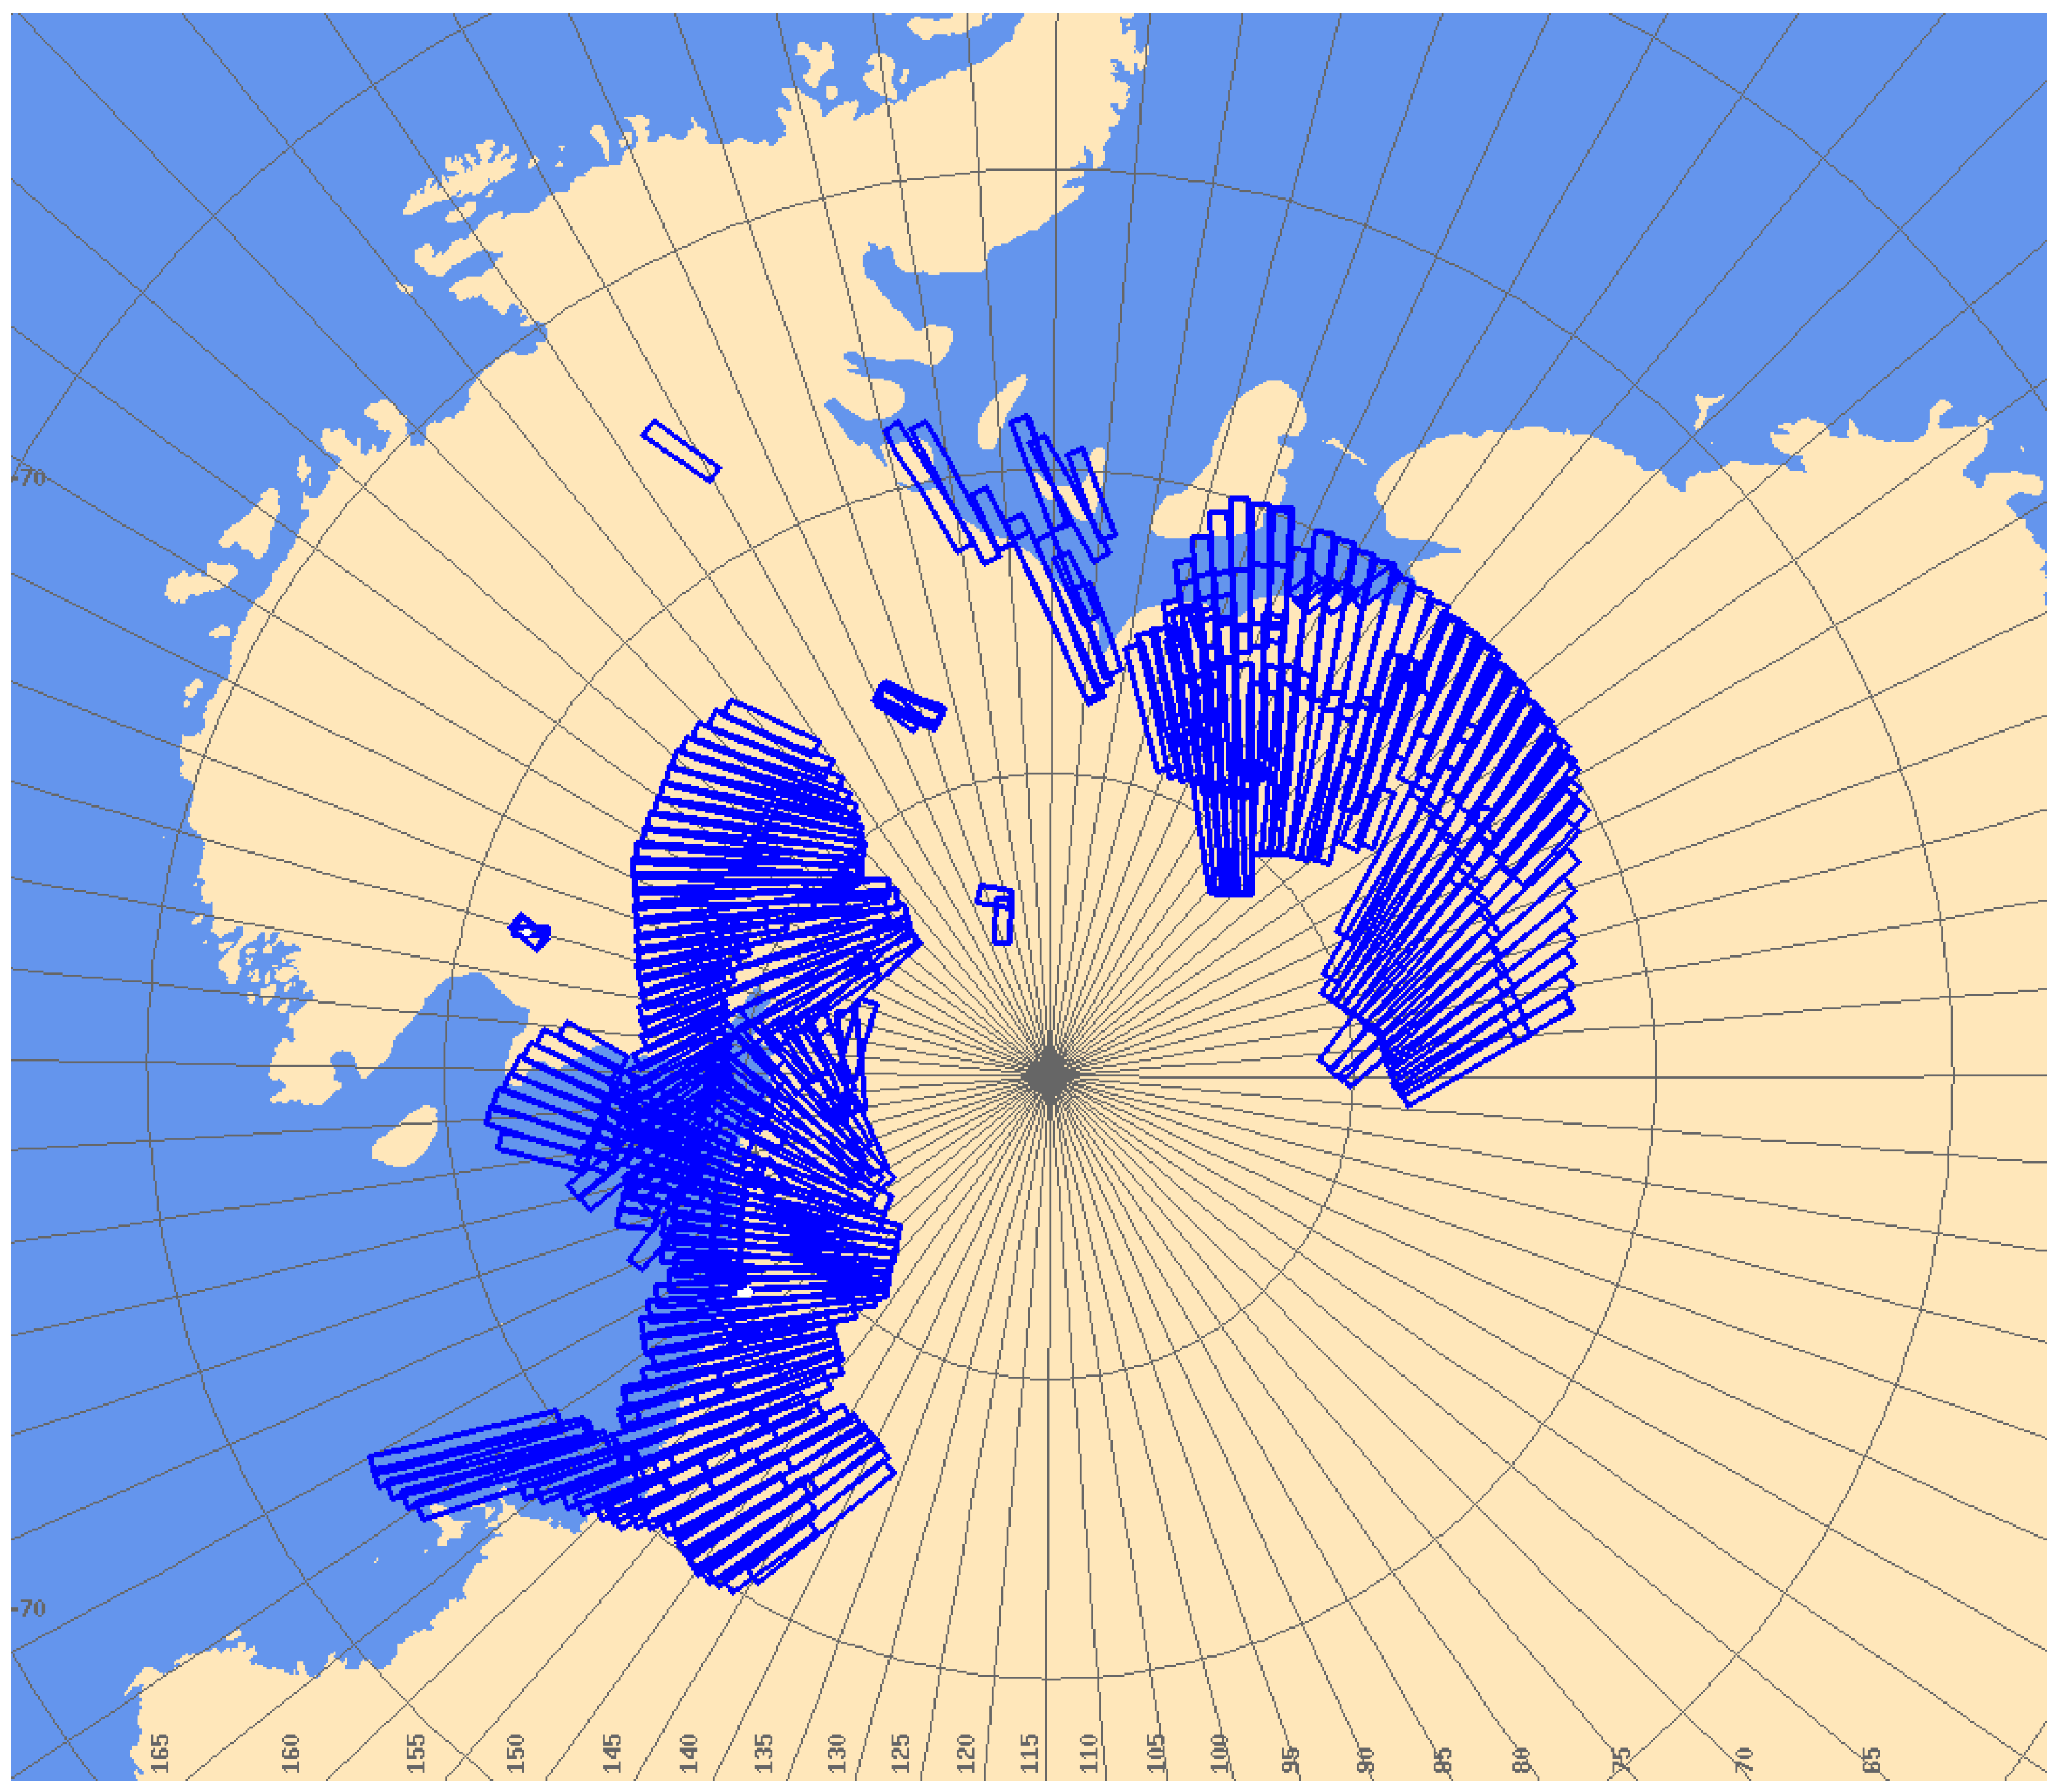
\includegraphics[width=.5\linewidth]{Figures/LiteratureReview/Satellites/TerraSAR_Antarctic_Acquisitions.png}
    \caption{Visualisation of the left-looking StripMap acquisitions over Antarctica requested from TerraSAR-X. Taken from \cite{Buckreuss2018}}
    \label{fig:litReview.sarCharac.satellites.terraSAR.antarcticStripmaps}
\end{figure}

Buckreuss et al. \cite{Buckreuss2018} and Pitz and Miller \cite{Pitz2010} mention the launch of a second satellite, TanDEM-X, in 2010. This satellite can be used to perform bistatic operations in tandem with TerraSAR-X \cite{Pitz2010, Buckreuss2018}. However, these analysis techniques and methods fall outside the scope of this project.

Overall, the TerraSAR-X mission has been successful in capturing \acs{sar} data over Antarctica and the \acs{so}, as depicted in Figure \ref{fig:litReview.sarCharac.satellites.terraSAR.antarcticStripmaps}, and it will be able to provide the desired data for this project.

\subsection{SAR Ocean Wave Inversion} \label{subsec:litReview.sarCharac.oceanWaveInversion}

In order to convert a \acs{sar} spectrum into an ocean-directional wave spectrum, two main conversion methods are employed. The first technique is the Hasselmann inversion technique, originally proposed by \ac{hh} \cite{Hasselmann1991} in 1991, and further improved upon in 1996 by Hasselmann et al. \cite{Hasselmann1996}. The second technique, which builds upon the Hasselmann inversion, was developed by Engen and Johnsen \cite{Engen1995} in 1995. The theory encompassing these inversion techniques, along with the related ocean and wave spectrum theory, is discussed in the chapter dedicated to theoretical development. This section will introduce the foundational aspects of these techniques, as well as their limitations. Subsequently, the following section will introduce the applications of these models in sea ice and wave modelling.

\subsubsection{Hasselmann Inversion Technique} \label{subsubsec:litReview.sarCharac.oceanWaveInversion.Hasselmann}

\ac{hh} developed a closed, nonlinear integral mapping transformation \cite{Wadhams2002}, which relates a \acs{sar} spectrum to a two-dimensional ocean-directional wave spectrum denoted as $F(\mathbf{k})$\footnote{$F(\mathbf{k})$ describes the distribution of wave energy with respect to the wave propagation number, $\mathbf{k}$. Further information about the two-dimensional wave spectrum is provided in the theoretical development chapter and can be found in \cite{Hasselmann1991, Holthuijsen2007}}. This wave spectrum enables the derivation of all statistical properties of an ocean wave field at any location and time \cite{Hasselmann1991}.

\ac{hh}'s inversion technique builds upon prior ocean inversion methods; however, these techniques were computationally inefficient and required a brute-force approach through the utilisation of Monte Carlo simulations\footnote{Monte Carlo simulations predict outcomes by employing estimated variable ranges and probability distributions. They iteratively generate results with various random numbers to produce a spectrum of likely scenarios.} for the statistical modelling of ocean waves using a pixel-by-pixel approach \cite{Hasselmann1991}.

\ac{hh} state that not all of the wave spectral information is mapped into the \acs{sar} image plane, and as such, they can only determine wave propagation direction to a specific sign \cite{Hasselmann1991}. Engen and Johsen \cite{Engen1995} overcome this limitation in the ways discussed in the following sub-section. This loss of information is due to two main issues. Firstly, the 180\,$^{\circ}$ propagation ambiguity\footnote{This ambiguity is due to the polarisation of the \acs{sar} waveform, as it does not allow the direction of the waves to be properly determined, i.e., whether they are travelling towards or away from a coastline or sea ice \cite{Fernandes2000}.}, and secondly, due to the nonlinear orbital motion of waves - particularly short waves and waves in windy oceans. This nonlinearity is known as velocity bunching and occurs due to fluctuations in the azimuthal displacements of image backscattering elements, caused by changing orbital velocities within the wave field \cite{Hasselmann1991}. The nonlinearity in this relationship stems from the interference between wave orbital velocities and the way in which \acs{sar} constructs its azimuthal resolution \cite{Mastenbroek2000}. \ac{hh} state that velocity bunching dominates over other nonlinearities and is the cause of smearing in the output \acs{sar} image spectrum \cite{Hasselmann1991}. This results in a loss of information for high wave numbers of the wave spectrum in the azimuthal direction \cite{Hasselmann1991, Hasselmann1996}.

In order to mitigate these nonlinearities, \ac{hh} adopts the approach of utilising a first-guess wave spectrum, derived from an existing model of the sea state. Using this initial guess spectrum, \ac{hh}'s technique aims to minimise a cost function for extracting the wave spectrum. \ac{hh} has discovered that iterative minimisation of this cost function leads to convergence within 3-4 iterations \cite{Hasselmann1991}. While this approach to mitigating nonlinearities proved successful, it requires prior knowledge of the sea state. Consequently, several researchers have attempted to address this limitation using various methods. For instance, Engen and Johnsen's \cite{Engen1995} image cross-spectra technique, which is discussed in the subsequent sub-section.

\subsubsection{Image Cross Spectra Inversion Technique} \label{subsubsec:litReview.sarCharac.oceanWaveInversion.Engen}

Building on the \ac{hh} inversion technique, Engen and Johnsen were able to mitigate the 180\,$^{\circ}$ propagation ambiguity without using an existing first-guess wave model \cite{Engen1995}. This was achieved using image cross spectra [I still don't understand this technique entirely so want to understand it more before writing about it. I want to follow a similar form to the above sub-section though: What the technique is, how it differs and improves on Hasselmann's, a basic overview of the difference in approach it takes, and any limitations to the method]

\subsection{Wave Propagation Model in Sea Ice} \label{subsec:litReview.sarCharac.seaIceWaveModelling}

The process of modelling sea ice and waves is achieved through the use of three wave attenuation and dispersion models \cite{DeCarolis2021, DeSanti2018}. These models are crucial to Antarctic science, as they enable the assessment of wave attenuation rate, spreading, and dispersion within sea ice, which are closely linked to the physical characteristics of the sea ice itself. This, in turn, allows for the inference of sea ice's physical characteristics \cite{DeCarolis2002}.

These three models are the Keller model, developed in 1998 by Keller \cite{Keller1998}; the two-layer viscous model, developed in 2002 by De Carolis and Desiderio \cite{DeCarolis2002}; and the close-packing model, developed in 2017 by De Santi and Olla \cite{DeSanti2017}. More information on these models can be found in the respective references. These models can then be used to infer properties of the sea ice region, such as pancake ice thickness and wave attenuation rate \cite{Aulicino2019}. This sub-section will introduce each of these models, discuss their results when applied following the definition of an open ocean wave spectrum using either of the inversion techniques described in the above sub-section and state the difficulties and inaccuracies found within these models.

\subsubsection{Keller Model} \label{subsubsec:litReview.sarCharac.seaIceWaveModelling.Keller}

The Keller model \cite{Keller1998} views the ice layer as a suspension with a higher viscosity than the water it sits on top of, as well as a density slightly less than that of the water. The sea ice is treated as a highly viscous incompressible liquid, whereas the water underneath it is treated as an inviscid\footnote{An inviscid liquid has negligible or zero viscosity.} incompressible liquid. This allows breaking the problem down into a two-layer problem, for which linear theory can be applied to solve the dispersion equation for waves entering a sea ice field \cite{Keller1998}. Keller's model relies heavily on the effective viscosity coefficient, $\mu(c)$, which differs for different ice types based on their shape and concentration. The model has only two free parameters: the viscosity and thickness of the sea ice. The best values for these are found by minimising the difference between the observed and simulated \acs{sar} spectrum \cite{Wadhams2004}.

Keller's model improves on the previously used mass loading model since, at high wave frequencies, it fits laboratory experiments by predicting an increase in wave wavelength upon entering the sea ice. Furthermore, Wadhams et al. \cite{Wadhams2004} also found that the inferred thickness using Keller's model showed excellent agreement between calculated ice thickness and the average ice thickness from in-situ measurements in the \acs{miz}.

\subsubsection{Two-layer Viscous Model} \label{subsubsec:litReview.sarCharac.seaIceWaveModelling.twoLayer}

The two-layer viscous model \cite{DeCarolis2002} builds upon Keller's model due to the limitations inherent in Keller's model, which is constrained by specific approximations. This extension incorporates wave attenuation rate and dispersion as functions of wave frequency. Additionally, it introduces an eddy viscosity for the water beneath the sea ice, contributing to improved accuracy. The emergence of this eddy viscosity stems from the consideration of turbulence at the interface between the sea ice and the ocean, particularly at the base of the ice layer in order to parameterise water flow underneath sea ice \cite{DeCarolis2002,DeSanti2018}.

%De Carolis and Desiderio \cite{DeCarolis2002} represent pancake ice as a layer of viscous fluid \cite{DeCarolis2002,Doble2015}. This viscosity of the ice layer governs various interactions that occur when waves cross a region covered by pancake ice. Such interactions include bending and collisions among individual pancakes \cite{Doble2015}. Analogous to Keller's model, the two-layer viscous model maintains the premise that the ice layer exhibits higher viscosity than the underlying ocean, and it acknowledges the influence of ice density, dependent on ice type and concentration \cite{DeCarolis2002,Doble2015}. The two-layer viscous model has good agreement with laboratory results with regard to observed wave attenuation and dispersion in grease ice \cite{DeCarolis2002}. However, De Carolis and Desiderio states that whilst the inclusion of an eddy viscosity holds scientific value, it needs to be modelled using more robust numerical methods.

De Carolis and Desiderio \cite{DeCarolis2002} represent pancake ice as a layer of viscous fluid \cite{DeCarolis2002,Doble2015}. This viscosity of the ice layer governs various interactions that occur when waves cross a region covered by pancake ice, including bending and collisions among individual pancakes \cite{Doble2015}. Analogous to Keller's model, the two-layer viscous model maintains the premise that the ice layer exhibits a higher viscosity than the underlying ocean, and it acknowledges the influence of ice density, which is dependent on ice type and concentration \cite{DeCarolis2002,Doble2015}. The two-layer viscous model demonstrates good agreement with laboratory results concerning observed wave attenuation and dispersion in grease ice \cite{DeCarolis2002}. However, De Carolis and Desiderio state that while the inclusion of an eddy viscosity holds scientific value, it needs to be modelled using more robust numerical methods for further validation.

\subsubsection{Close-Packing Model} \label{subsubsec:litReview.sarCharac.seaIceWaveModelling.CP}

[Still reading about this model. I want to follow a similar form to the two above subsections though. My idea is: The model it builds on and how it differs from this model (Any reasons for these choices in changes and improvements), a brief overview of how the model works, and any negatives to this approach when studied in comparison to in-situ measurements]

%****************************************************
% END
%****************************************************
%****************************************************
%	CHAPTER 3 - THEORETICAL DEVELOPMENT
%****************************************************
\chapter{Theoretical Background}
\label{chap:theory}
In order to understand the \ac{hh} inversion technique, the theoretical foundations surrounding the modelling of ocean waves, in both deep and shallow water, need to be understood. Furthermore, a foundational understanding of \ac{sar}, encompassing its data acquisition and types, along with the pre-processing techniques applied in implementing the \ac{hh} technique to achieve the desired outcomes, is necessary.

This chapter's objective is to introduce the theoretical aspects surrounding these fields, thereby providing context for the subsequent chapter's introduction of the pipeline design. Additionally, this chapter builds upon the theories previously discussed in Chapter \ref{chap:litReview}. In this chapter, key terms are useful to enhance the understanding of the reader. Field-specific terms are briefly introduced in the \nameref{chap:glossary} and provide context to the terms used in the subsequent sections.

%====================================================
% OCEAN WAVES
%====================================================
\section{Ocean Waves} \label{sec:theory.waves}
The majority of this section draws upon content collated by Holthuijsen \cite{Holthuijsen2007}, with equations and figures cited appropriately. The objective of this section is to provide an introductory overview of the fundamental theory related to ocean waves and their mathematical modelling as well as highlighting the differences in this modelling in deep and shallow water. Appropriate, and relevant derivations and visual explanations of key concepts are included in Appendix \ref{ap:oceanWaves}. %Furthermore, the way in which waves are attenuated and dispersed upon entering the \ac{miz} in Antarctica is discussed.

\subsection{Description of Ocean Waves} \label{subsec:theory.waves.description}

The wave height, $H$, can be defined as the vertical distance between the lowest and highest surface elevation in a wave. Where surface elevation, denoted using $\eta(t)$, refers to the instantaneous elevation of the sea surface relative to some reference level. The zero-crossing wave period, $T_{0}$, can be defined as the time between one zero-down crossing and the following one. Where a zero-down crossing is the crossing of the mean surface elevation when the gradient of the wave is negative. All of these terms are depicted in Figure \ref{fig:theory.waves.introFigure}.

\begin{figure}[H]
    \centering
    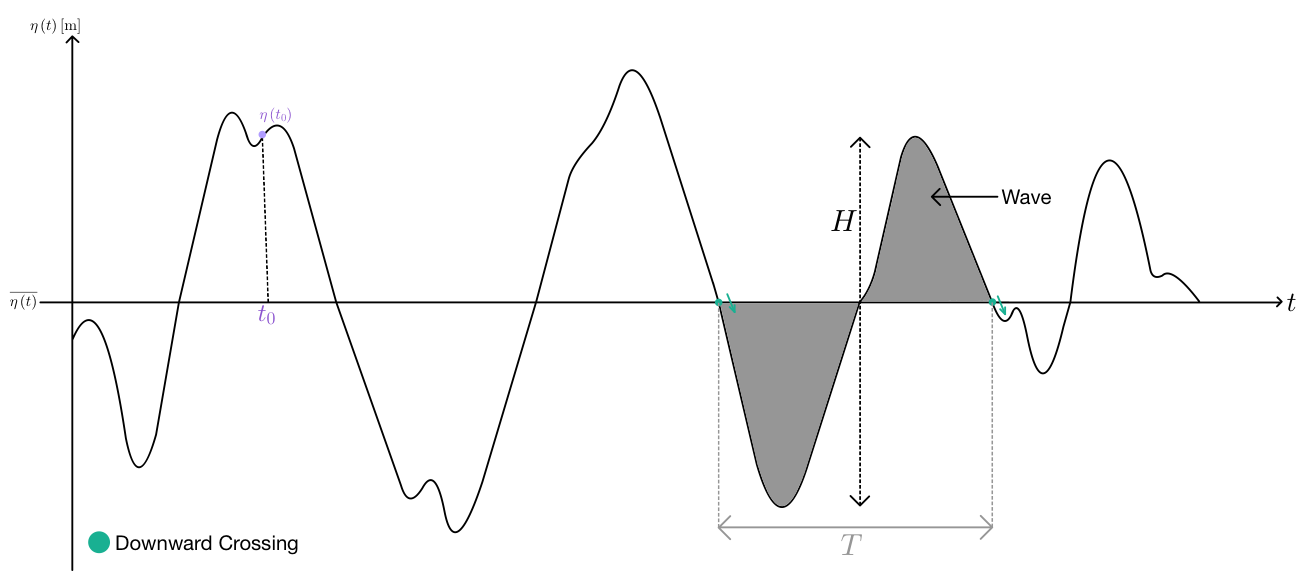
\includegraphics[width=.8\linewidth]{Figures/Theory/placeholder_waveDefinitions.png}
    \caption{Visual definition of surface elevation ($\eta(t)$), wave height ($H$), wave period ($T$), and zero-down crossing. Adapted from \cite{Holthuijsen2007}.}
    \label{fig:theory.waves.introFigure}
\end{figure}

Holthuijsen \cite{Holthuijsen2007} defines the following equations for the mean wave height and zero-crossing wave period for $N$ wave where $i$ represents the sequence number of the waves in the \gls{waveRecord}.

\begin{equation} \label{eq:waves.mean(H)}
    \overline{H} = \frac{1}{N}\sum_{i}^{N}H_{i}
\end{equation}

\begin{equation} \label{eq:waves.mean(T0)}
    \overline{T_{0}} = \frac{1}{N}\sum_{i}^{N}T_{0,i}
\end{equation}

The definition of the significant wave height and wave period follows, where $j$ is the rank number of the sequence of waves, based on wave height, in descending order. The significant wave height is a useful metric, as it can be estimated from the wave spectrum \cite{Holthuijsen2007}, which is introduced in the subsequent subsection.

\begin{equation} \label{eq:waves.sigH}
    H_{1/3} = \frac{1}{N/3}\sum_{j}^{N/3}H_{j}
\end{equation}

\begin{equation} \label{eq:waves.sigT}
    T_{1/3} = \frac{1}{N/3}\sum_{j}^{N/3}T_{0,j}
\end{equation}

\subsection{Wave Spectra} \label{subsec:theory.waves.waveSpectrum}
Include info about stationary measurements
\subsubsection{Random Phase/Amplitude Model} \label{subsec:theory.waves.waveSpectrum.randModel}

The wave spectrum aims to describe the ocean surface as a stationary stochastic process\footnote{define stochastic process}. It is based on the random-phase/amplitude model, where the surface elevation is treated as the sum of a large number of harmonic waves. Each of these waves possesses a constant amplitude and a phase that is randomly selected for each time record realisation. This approach enables the modelling of the wave spectrum as a Fourier series, as illustrated in Equation \ref{eq:waveSpectrum.fourierSeries}. For a more detailed explanation, please refer to Appendix \ref{sec:ap.oceanWaves.randModel}.

\begin{equation} \label{eq:waveSpectrum.fourierSeries}
    \underline{\eta}(t) = \sum_{i=1}^{N}\underline{a}_{i}cos(2\pi f_{i}t + \underline{\phi}_{i})
\end{equation}

ADD NOTES ON APPLICABILITY OF RANDOM MODEL (pg. 35 - beginning 36)

\subsubsection{Variance Density Spectrum} \label{subsec:theory.waves.waveSpectrum.varianceSpectrum}

The variance density spectrum can be constructed by utilising the variance, $E\left \{  \frac{1}{2}\underline{a}^{2}_{i}\right \}$, as opposed to the expected value, $E\left \{  \underline{a}_{i}\right \}$. [Use note 3A to explain variance] Also explain why variance is better than using expected value [variance is chosen as it allows the change over different samples to be seen, as opposed to the pure magnitude.]
% This choice to use variance is preferred as it allows changes across different samples to be observed, rather than each sample's pure magnitude.

In order to mitigate the second issue with the application of the random phase/amplitude model, it is modified by distributing the variance over the frequency interval $\Delta f_{i}$ and the frequency $f_{i}$. This gives rise to the variance \textbf{density} spectrum, $E^{*}\left \{ \frac{1}{2}  \underline{a}^{2}_{i}\right \}$.


\begin{equation} \label{eq:waveSpectrum.varianceDSpectrum}
    E^{*}\left \{  f_{i}\right \} = \frac{1}{\Delta f_{i}}E\left \{\frac{1}{2}  \underline{a}^{2}_{i}\right \} \; \; \; \text{for all} \; \; \;  f_{i}
\end{equation}

Whilst Equation \ref{eq:waveSpectrum.varianceDSpectrum} is defined for all frequencies, it is still discontinuous between frequency bands. A continuous version of $E^{*}\left \{  f_{i}\right \}$ can be determined by taking the limit as $\Delta f_{i}$ tends to zero. This entire process is graphically depicted in Figure \ref{fig:theory.waves.waveSpectrum.varianceDSpectrum}.

\begin{equation} \label{eq:waveSpectrum.varianceDSpectrumCont}
    E(f) = \lim_{\Delta f \to 0}\frac{1}{\Delta f}E\left \{ \frac{1}{2} \underline{a}^{2}\right \}
\end{equation}
[Show graphically with FIG 3.7 - pg. 37]

\begin{figure}[H]
    \centering
    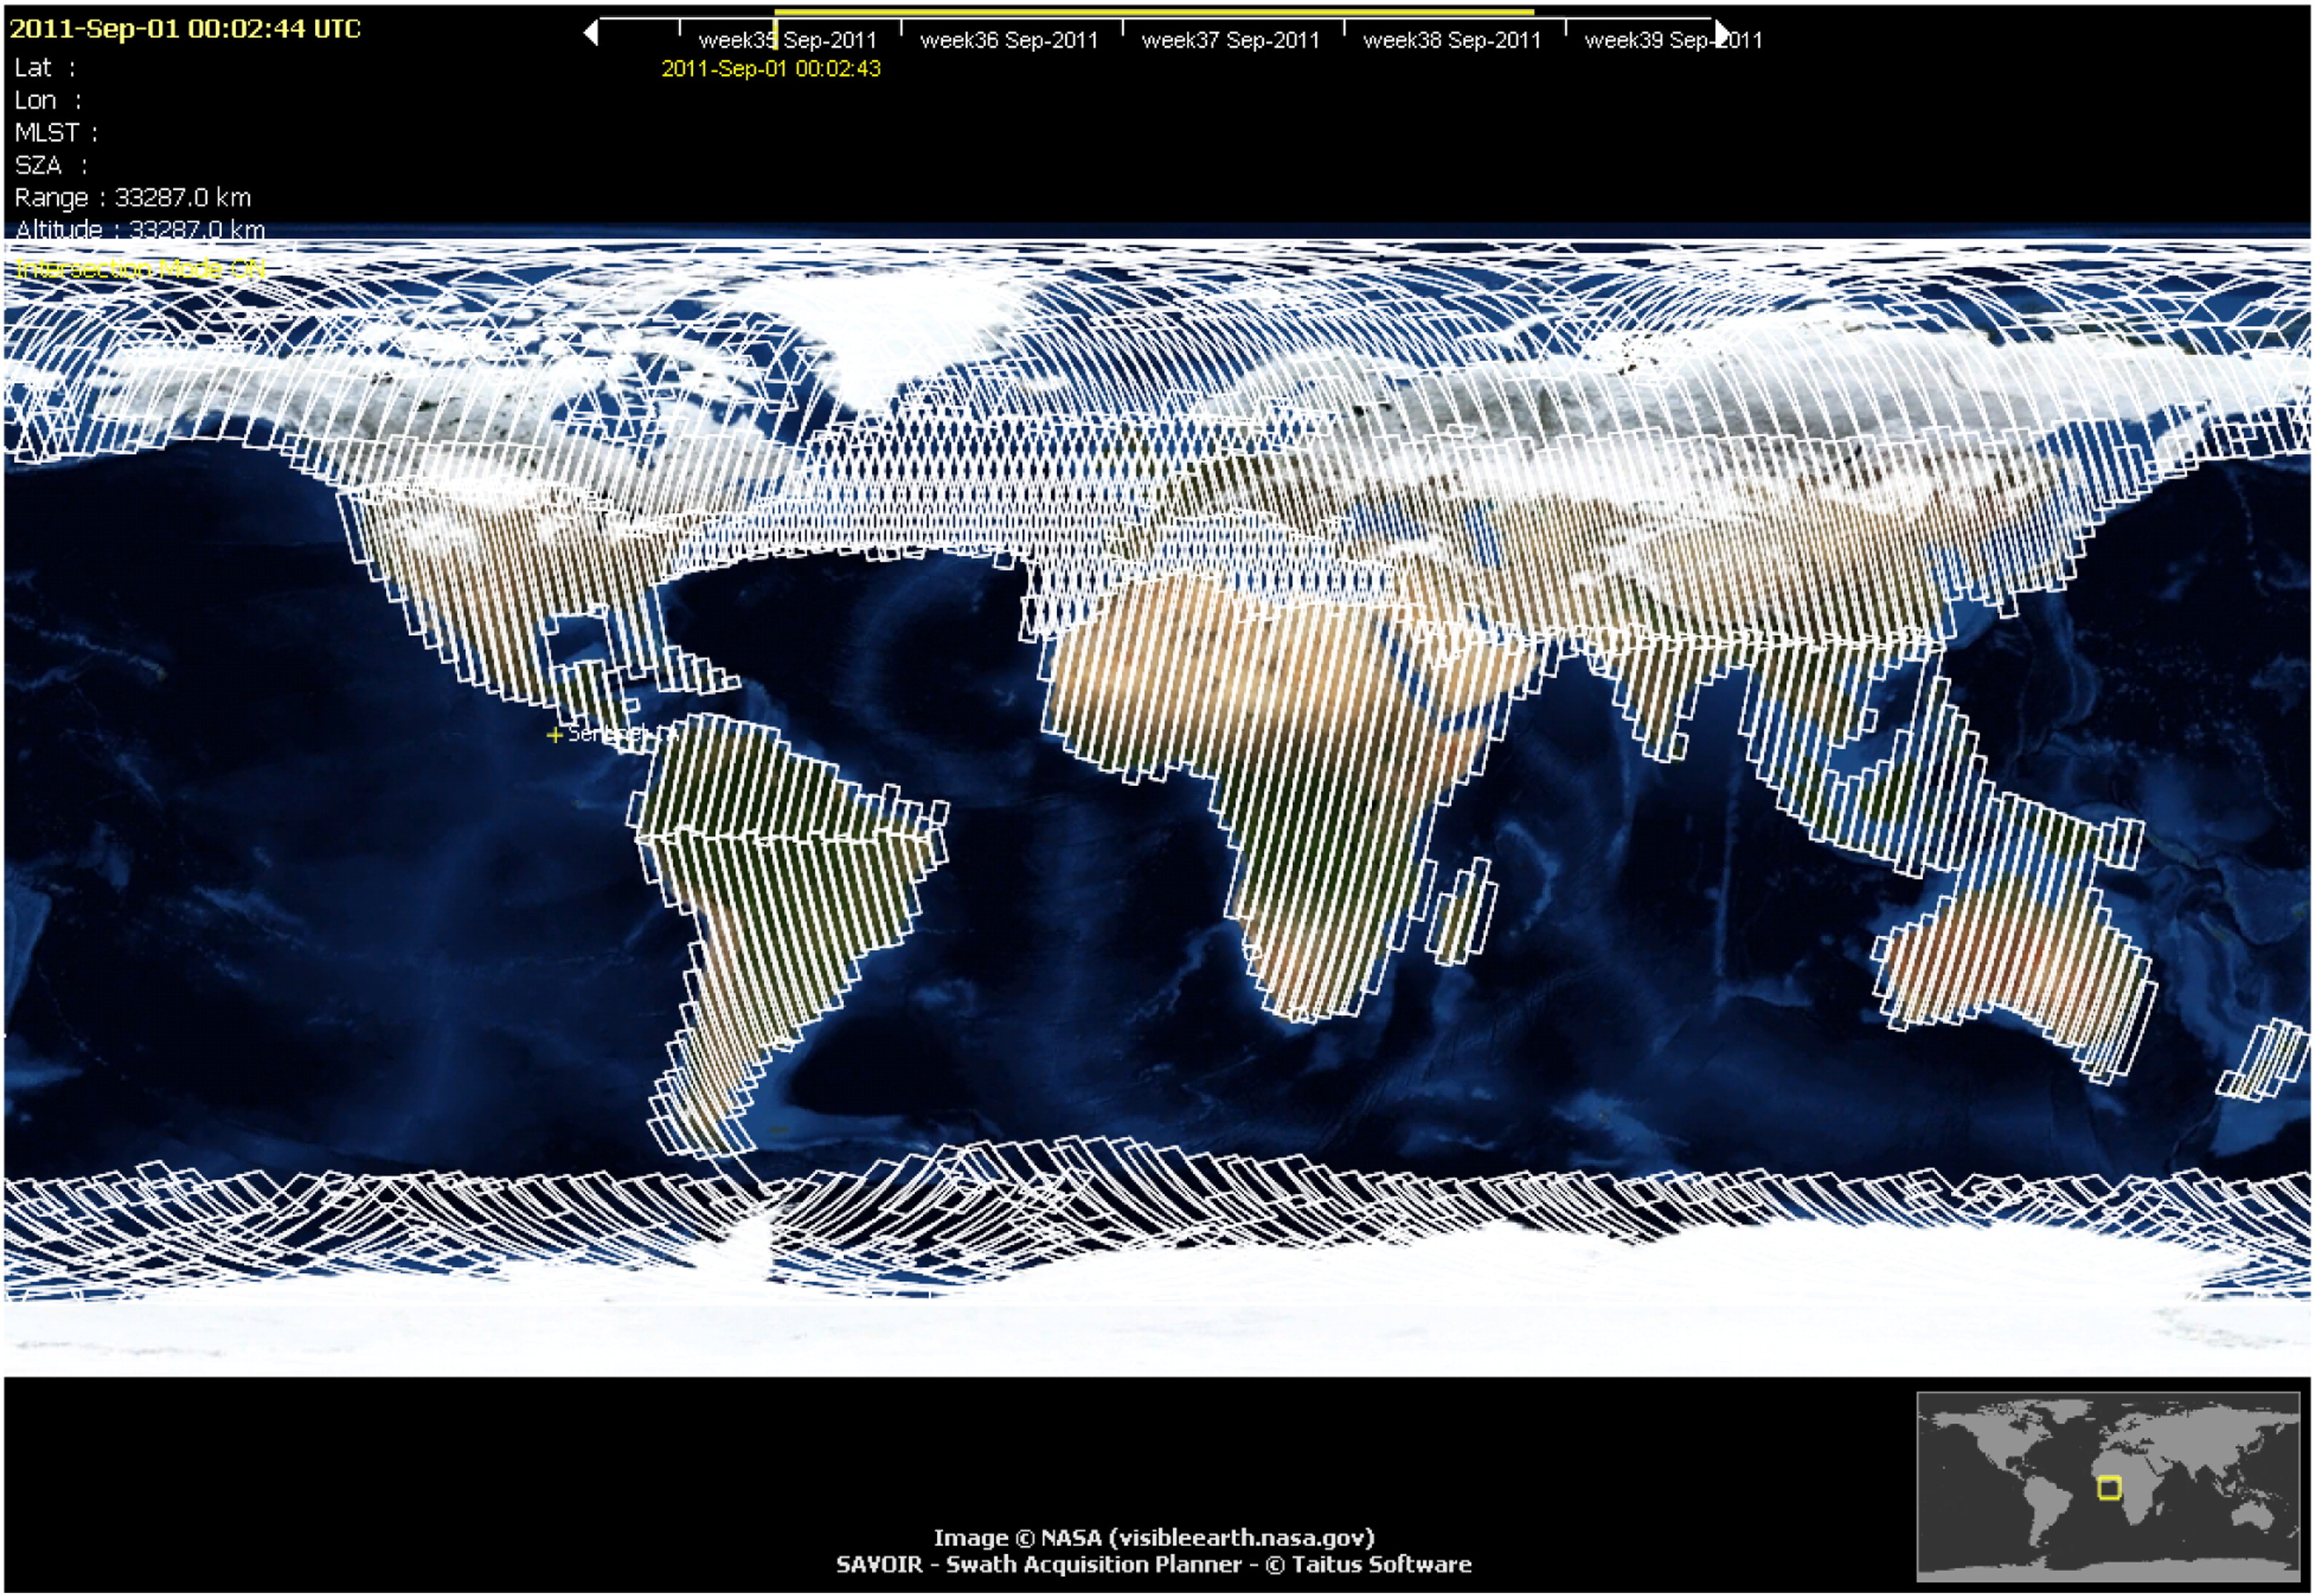
\includegraphics[width=.5\linewidth]{Figures/LiteratureReview/Satellites/sentinelCoverage.jpg}
    \caption{Visual explanation of the transformation from discrete amplitude spectrum of the random phase/amplitude model (top frame), depicted in Figure \ref{fig:ap.randModel}, to the continuous variance density spectrum (bottom frame). Adapted from \cite{Holthuijsen2007}.}
    \label{fig:theory.waves.waveSpectrum.varianceDSpectrum}
\end{figure}

The variance density spectrum provides a complete description of the surface elevation of ocean waves as all statistical characteristics of the wave field can be expressed in terms of this spectrum, provided it is modelled as a stationary, Gaussian process.

% The units of the variance density spectrum, $E(f)$, can be derived as follows.
% \begin{gather*}
%     \frac{1}{\Delta f}E\left \{ \frac{1}{2} \underline{a}^{2}\right \} \; \; \; \text{has units:}\\
%     \frac{1}{\text{s}^{-1}}\text{m}^{2} = \text{m}^{2}\text{s} = \text{m}^{2}/\text{Hz}
% \end{gather*}

% The allows the total variance, $\overline{\underline{\eta}^{2}}$, to be calculated as follows.

% \begin{equation} \label{eq:waveSpectrum.totalVar}
%     \overline{\underline{\eta}^{2}} = \int_{0}^{\infty} E(f)df
% \end{equation}


\subsubsection{Spectral Domain Definition} \label{subsec:theory.waves.waveSpectrum.spectralDef}
Equations \ref{eq:waveSpectrum.fourierSeries},\ref{eq:waveSpectrum.varianceDSpectrumCont} are defined in terms of time and frequency. In order to represent the variance density spectrum in the radian frequency, $\omega$, the relationship, $\omega = 2\pi/T$ needs to be used. Equation \ref{eq:waveSpectrum.fourierSeries} is then updated to the following form

\begin{equation} \label{eq:waveSpectrum.fourierSeries_omega}
    \underline{\eta}(t) = \sum_{i=1}^{N}\underline{a}_{i}cos(\omega t + \underline{\phi}_{i})
\end{equation}

This allows the variance density spectrum, $E(\omega)$, to be defined as follows, where $J$ represents the Jacobian. In this case, $J=1/2\pi$.
\begin{equation} \label{eq:waveSpectrum.relateE(f)toE(w)}
    E(\omega) =  E(f) \frac{df}{d\omega} = E(f)J = \frac{1}{2\pi}E(f)
\end{equation}

\subsubsection{Frequency-direction Spectrum} \label{subsec:theory.waves.waveSpectrum.freqDirection}
The variance density spectrum equation as described in Equation \ref{eq:waveSpectrum.varianceDSpectrumCont} represents a one-dimensional function of time. In order to consider a two-dimensional spectrum, the random phase/amplitude model needs to be expanded to consider a wave propagating in the $x,y$-space in a direction $\theta$, relative to the +$x$-axis. This allows the model to be expanded as follows, where the wave number, $k = 2\pi/L$ with $L$ equal to the length of the harmonic wave.

\begin{equation} \label{eq:waveSpectrum.fourierSeries_3D}
    \underline{\eta}(x,y,t) = \sum_{i=1}^{N} \sum_{j=1}^{M} \underline{a}_{i,j}cos(\omega_{i}t-k_{i}xcos(\theta_{j}) - k_{i}ysin(\theta_{j}) + \underline{\phi}_{i,j})
\end{equation}

where each wave component is indicated by two indices.
\begin{itemize}
    \item $i$: The frequency index or wave number
    \item $j$: The direction
\end{itemize}

Following the same process of transforming a one-dimensional amplitude spectrum into a continuous variance density spectrum, as detailed in Equations \ref{eq:waveSpectrum.varianceDSpectrum}, \ref{eq:waveSpectrum.varianceDSpectrumCont}, the two-dimensional variance density spectrum is found as

\begin{equation} \label{eq:waveSpectrum.varianceDSpectrumCont_2D}
    E(\omega,\theta) =  \lim_{\Delta \omega \to 0}\lim_{\Delta \theta \to 0}\frac{1}{\Delta \omega \Delta \theta} E\left \{ \frac{1}{2} \underline{a}^{2}\right \}
\end{equation}

Using the Jacobian determined in Equation \ref{eq:waveSpectrum.relateE(f)toE(w)}, the same relationship can be developed for the two-dimensional variance density spectrum

\begin{equation} \label{eq:waveSpectrum.relateE(f)toE(w)_2D}
    E(\omega,\theta) =  \frac{1}{2\pi}E(f,\theta)
\end{equation}

\subsection{Wave-number Spectra} \label{subsec:theory.waves.waveNumberSpectra}
Where the wave spectrum considers the sea as a function of space and time, $\eta(x,y,t)$, the ocean can also be considered as a function of space at a single moment in time. This idea is useful for remote sensing applications.

% \subsubsection{One-dimensional spectrum} \label{subsec:theory.waves.waveNumberSpectra.1D}
% The definition of the one-dimensional wave-number spectrum is identical to the frequency-direction spectrum, however, the time is replaced by the horizontal coordinate, $x$, and the radian frequency is replaced by the wave number, $k$. This allows $E(k)$ to be defined as the following, where $\Delta k$ is the wave-number bandwidth.

% \begin{equation} \label{eq:waveNumberSpectrum.E(K)_1D}
%     E(k) = \lim_{\Delta k \to 0} \frac{1}{\Delta k} E\left \{ \frac{1}{2} \underline{a}^{2}\right \}
% \end{equation}

% In order to transform the wave-number spectrum into the frequency spectrum the following formula can be used. The Jacobian is found to be $c_{g}$, the velocity at which the waves propagate.

% \begin{equation} \label{eq:waveNumberSpectrum.relateE(f)toE(w)_1D}
%     E(k) =  E(\omega) \frac{d\omega}{dk} = c_{g}E(\omega)
% \end{equation}

\subsubsection{Two-dimensional spectrum} \label{subsec:theory.waves.waveNumberSpectra.2D}
In order to define the two-dimensional wave-number spectrum, the method described in Equations \ref{eq:waveSpectrum.fourierSeries}, \ref{eq:waveSpectrum.varianceDSpectrumCont} can be used. Where $\Delta k_{x}$ and $\Delta k_{y}$ represent the spectral bandwidths.

\begin{equation} \label{eq:waveNumberSpectrum.fourierSeries_2D}
    \eta(x,y) = a_{i,j}cos(k_{x,i}x + k_{y,j}y + \phi_{i,j})
\end{equation}

\begin{equation} \label{eq:waveNumberSpectrum.SpectrumCont_2D}
    E(k_{x},k_{y}) = \lim_{\Delta k_{x} \to 0} \lim_{\Delta k_{y} \to 0} \frac{1}{\Delta k_{x} \Delta k_{y}} E\left \{ \frac{1}{2} \underline{a}^{2}\right \}
\end{equation}

With $k_{x} = k\cos(\theta)$, and $k_{y} = k\sin(\theta)$, $k$ and $\theta$ can be defined as: $k = \sqrt{k_{x}^2 + k_{y}^2}$ and $\theta = \text{arctan}(k_{y}/k_{x})$. This allows an equivalent spectrum to be defined in terms of $k$ and $\theta$.

\begin{equation} \label{eq:waveNumberSpectrum.SpectrumCont_2D_kTh}
    E(k,\theta) = \lim_{\Delta k \to 0} \lim_{\Delta \theta \to 0} \frac{1}{\Delta k \Delta \theta} E\left \{ \frac{1}{2} \underline{a}^{2}\right \}
\end{equation}

These two spectra are related by the following relationship.
\begin{equation} \label{eq:waveNumberSpectrum.relateE(k,th)toE(kx,ky)_2D}
    E(k,\theta) =  E(k_{x},k_{y}) J = k E(k_{x},k_{y})
\end{equation}

The two-dimensional frequency-direction spectrum in Equation \ref{eq:waveSpectrum.varianceDSpectrumCont_2D} is related to the spectrum in Equation \ref{eq:waveNumberSpectrum.SpectrumCont_2D} by the following relationship, where $c_{w} = \omega /k$ and the Jacobian, $J = 1/c_{g}$. $c_{w}$ and $c_{g}$ are defined as the wave speed and group wave speed respectively and are discussed in the following subsection.
\begin{equation} \label{eq:waveNumberSpectrum.relateE(kx,ky)toE(w,th)_2D}
    E(k_{x},k_{y}) =  k E(\omega,\theta) J = \frac{c_{w} c_{g}}{\omega} E(\omega,\theta)
\end{equation}

These two-dimensional spectra are useful in two different applications, however, in varying forms.
\begin{itemize}
    \item Remote sensing: $E(k_{x},k_{y})$
    \item Wave models: $E(f,\theta)$
\end{itemize}

\subsection{Linear Wave Theory} \label{subsec:theory.waves.linearWaveTheory}

The linear theory for \gls{oceanWaves} provides a detailed description of harmonic waves. It relies on two equations and associated boundary conditions, which are discussed in Chapter 5.3 of \cite{Holthuijsen2007}. The solution to the kinematic boundary conditions results in a wave propagating in the $x$-direction. This propagating harmonic can be described in two different ways.

\begin{subequations}  \label{eq:linearWaveTheory.propHarmonicWave}
  \begin{align}
    \eta(x,t) = a\text{sin}(\omega t - kx) \\
    \eta(x,t) = \frac{H}{2}\text{sin} \left ( \frac{2\pi}{T}t - \frac{2\pi}{L}x \right )
  \end{align}
\end{subequations} 


\begin{itemize}
    \item Illustration on page 119
\end{itemize}

% Include derivation of c_wave - page 119

\subsection{Ocean Wave Dynamics} \label{subsec:theory.waves.dynamics}

Considering the harmonic surface profile of ocean waves, as well as the velocity potential function, which are described by Holthuijsen in Chapter 5.4.2 \cite{Holthuijsen2007}, a relationship, known as the dispersion relationship can be developed.

\subsubsection{Dispersion Relationship} \label{subsec:theory.waves.dynamics.dispersionRelationship}

The dispersion relationship relates the radian frequency, $\omega$, to the wave number, $k$ \cite{Holthuijsen2007}. The dispersion relationship for an arbitrary depth is given as 

\begin{equation} \label{eq:linearWaveTheory.dispersionRelationship}
    \omega ^2 = gk\text{tanh}(kd).
\end{equation}

The propagation speed of a wave can be determined from Equation \ref{eq:linearWaveTheory.dispersionRelationship} with the fact that $c_{w} = \omega / k$. This gives the wave phase speed for an arbitrary depth as

\begin{equation} \label{eq:linearWaveTheory.phaseVelocity}
    c_{w} = \frac{g}{\omega}\text{tanh}(kd) = \sqrt{\frac{g}{k}\text{tanh}(kd)}
\end{equation}

Considering Equation \ref{eq:linearWaveTheory.dispersionRelationship} and \ref{eq:linearWaveTheory.phaseVelocity} for both deep water and shallow water yields the following approximations to be determined.

\subsubsection{Deep Water} \label{subsec:theory.waves.linearWaveTheory.deepWater}

In deep water, the term, $kd \to \infty$, and due to this, $\text{tanh}(kd) \to 1$ \cite{Holthuijsen2007}. This means that the dispersion relationship for deep water approaches

\begin{equation} \label{eq:linearWaveTheory.dispersionRelationship.deepWater}
    \omega_{0} = \sqrt{gk_{0}}
\end{equation}

where $k_0$ is the deep water wave number. The same logic with respect to $kd \to \infty$ applies to the phase velocity and means that the deep water phase velocity reduces to 

\begin{equation} \label{eq:linearWaveTheory.phaseVelocity.deepWater}
    c_{w_0} = \sqrt{\frac{g}{k_{0}}} = \frac{g}{\omega_{0}}  = \frac{g}{2\pi}T
\end{equation}

\subsubsection{Shallow Water} \label{subsec:theory.waves.linearWaveTheory.shallowWater}

In shallow water, the term, $kd \to 0$, and due to this, $\text{tanh}(kd) \to kd$ \cite{Holthuijsen2007}. This means that the dispersion relationship for shallow water approaches

\begin{equation} \label{eq:linearWaveTheory.dispersionRelationship.shallowWater}
    \omega = k\sqrt{gd}
\end{equation}

The same logic with respect to $kd \to 0$ applies to the phase velocity and means that the shallow water phase velocity reduces to 

\begin{equation} \label{eq:linearWaveTheory.phaseVelocity.shallowWater}
    c_{w_{shallow}} = \sqrt{gd}
\end{equation}

Equation \ref{eq:linearWaveTheory.phaseVelocity.shallowWater} shows that the phase speed does not depend on wavelength or frequency, and as such, this means that the waves are non-dispersive\footnote{non-dispersive defn.}.

\subsubsection{Adding Two Harmonic Waves} \label{subsec:theory.waves.linearWaveTheory.twoHarmonicWaves}

Using the definition of a propagating harmonic wave in Equation \ref{eq:linearWaveTheory.propHarmonicWave}, two of these waves can be combined in the following form.

\begin{equation} \label{eq:addingTwoWaves}
    \eta = \eta_{1} + \eta_{2} = a\text{sin}(\omega_{1}t - k_{1}x) + a\text{sin}(\omega_{2}t - k_{2}x)
\end{equation}

These two waves combine to create a sequence of wave groups. This group reaches its peak surface elevation when both $\eta_{1}$ and $\eta_{2}$ are in phase with each other. The phase velocity of these waves can be defined as the phase speed of the surface elevation envelope. This envelope can be determined by re-arranging Equation \ref{eq:addingTwoWaves} to give

% Fix with \left and \right
\begin{equation} \label{eq:addingTwoWaves.envelopeForm}
    \eta =  2a\text{cos} \left ( \frac{\omega_{1} - \omega_{2}}{2}t - \frac{k_{1} - k_{2}}{2}x \right ) \text{sin} \left ( \frac{\omega_{1} + \omega_{2}}{2}t - \frac{k_{1} + k_{2}}{2}x  \right )
\end{equation}

The cosine term acts as the envelope, while the sine term acts as the carrier wave \cite{Holthuijsen2007}. The phase velocity of the envelope represents the velocity of the wave group and can be derived as

\begin{equation} \label{eq:addingTwoWaves.envelopeVelocity}
    c_{envelope} = c_{g} = \frac{(\omega_{1} + \omega_{2})/2}{(k_1 + k_2)/2} = \frac{\Delta \omega}{\Delta k}
\end{equation}

As the frequencies and wave numbers can be considered as continuous, Equation \ref{eq:addingTwoWaves.envelopeVelocity} can be redefined as

\begin{equation} \label{eq:addingTwoWaves.groupVelocity}
    c_{g} = \frac{\partial \omega}{\partial k} = nc_{w}
\end{equation}

where $n$ is derived from Equation \ref{eq:linearWaveTheory.dispersionRelationship} as 

\begin{equation} \label{eq:addingTwoWaves.n}
    n = \frac{1}{2} \left ( 1+ \frac{2kd}{\text{sinh}(2kd)} \right )
\end{equation}

This value for $n$ varies between $\frac{1}{2}$ for deep water ($kd \to \infty$), and 1 for shallow water \cite{Holthuijsen2007} ($kd \to 0$) and implies that $c_{w} \geq c_{g}$. 

\subsection{Wave Modelling for Idealised Cases} \label{subsec:theory.waves.modelling}

\subsubsection{One-dimensional Wave Spectrum} \label{subsubsec:theory.waves.modelling.1D}

The one-dimensional wave spectrum has been significantly advanced by the \acf{jonswap}, which is the most widely employed spectrum for wave modelling \cite{Holthuijsen2007}. This spectrum builds upon the Pierson-Moskowitz spectrum \cite{Pierson1964}, which models a fully developed spectrum in deep water. It expands upon the Pierson-Moskowitz spectrum by incorporating its spectral shape and introducing a peak enhancement factor denoted as $G(f)$ \cite{Hasselmann1973JONSWAP,Hasselmann1974JONSWAP}.

The Pierson-Moskowitz spectrum is defined as

\begin{equation} \label{eq:piersonMoskowitz}
    E_{PM} (f) = \alpha g^{2}(2\pi)^{-4}f^{-5}\text{exp} \left [ -\frac{5}{4} \left ( \frac{f}{f_{peak}}\right ) ^{4} \right]
\end{equation}

which results in the derivation of the \acs{jonswap} spectrum as

\begin{equation} \label{eq:jonswap.itoPiersonMoskowitz}
    E_{JONSWAP} (f) = E_{PM} (f) \, G(f)
\end{equation}

where 

\begin{equation} \label{eq:jonswap.peakEnhancementFactor}
    G(f) = \gamma ^{\text{exp} \left [  - \frac{1}{2} \left ( \frac{f/f_{peak}^{-1}}{\sigma} \right )^2 \right ]}
\end{equation}

$\gamma$ is the peak enhancement factor and is determined experimentally for the specific region over which waves need to be modelled. $\sigma$ is the peak width parameter which varies between $\sigma_{a}$ and $\sigma_{b}$ for the following conditions \cite{Holthuijsen2007}:

\begin{equation*}
  \sigma =
    \begin{cases}
      \sigma_{a} = 0.07 & \text{for $f \leq f_{peak}$}\\
      \sigma_{b} = 0.09 & \text{for $f > f_{peak}$}\\
    \end{cases}       
\end{equation*}

$\alpha$ is called the energy scale parameter and is calculated using the significant wave height and peak frequency

\begin{equation} \label{eq:jonswap.alpha}
    \alpha = 0.2 \frac{H_{1/3}^2 f_{peak}^{4}}{g^{2}}
\end{equation}

\begin{itemize}
    \item Show adapted Figure 6.6 (page 161)
\end{itemize}

\subsubsection{Two-dimensional Wave Spectrum} \label{subsubsec:theory.waves.modelling.2D}

To extend one-dimensional wave models generated using the \acs{jonswap} spectrum to two dimensions, the introduction of a directional distribution function is required. This directional distribution function represents the cross-section of the two-dimensional spectrum at a specific frequency and is normalised so that the integral of the function over its distribution equals one \cite{Holthuijsen2007}. It is a function of both $\theta$ and frequency but is often simply denoted as $D(\theta)$. The directional distribution employs a $\cos^{2}\theta$ model \cite{Holthuijsen2007} and takes the form

\begin{equation} \label{eq:directionalDistributionFunc}
    D(\theta) = A_{2} \cos^{2s} \left ( \frac{1}{2} (\theta_{wave} - \theta_{wind}) \right )
\end{equation}

where $A_{2}$ is determined using the gamma function\footnote{Gamma function definition}, $\Gamma(\cdot)$, and $s$ controls the distribution's width. 

\begin{equation} \label{eq:directionalDistributionFunc.A2}
    A_{2} = \frac{\Gamma(s+1)}{\Gamma \left ( s + \frac{1}{2} \right )2\sqrt{\pi}}
\end{equation}

and $s$ is related to the directional width, $\sigma_{\theta}$ by

\begin{equation} \label{eq:directionalDistributionFunc.sigTh}
    s = \frac{2}{\sigma_{\theta}^{2}} - 1
    %\sigma_{\theta} = \sqrt{\frac{2}{s + 1}} \text{[rad]}
\end{equation}

A reasonable approximation for $\sigma_{\theta}$ is given by

\begin{equation*}
  \sigma_{\theta} =
    \begin{cases}
      26.9 \left ( \frac{f}{f_{peak}} \right ) ^{-1.05} & \text{for $f < f_{peak}$}\\
      26.9 \left ( \frac{f}{f_{peak}} \right ) ^{0.68} & \text{for $f \geq f_{peak}$}\\
    \end{cases}       
\end{equation*}


%%%%%%%%%%%%%%%%%%%%%%%%%%%%%%%%%%%%%%%%%%%%%%%%%%%%
% ocean waves from glossary: \gls{oceanWaves}
% Chap. 5:
% Idealisations (N.B.)

% Chap. 6:
% [Look at key concepts]
% significant wave height:
% \begin{equation} \label{eq:waves.deepWater.sigH}
%     \Tilde{H}_{1/3} = \frac{gH_{1/3}}{U^{2}_{10}}
% \end{equation}


% significant wave period:
% \begin{equation} \label{eq:waves.deepWater.sigT}
%     \Tilde{T}_{1/3} = \frac{gT_{1/3}}{U_{10}}
% \end{equation}

% Assume waves stop growing when phase speed of waves approaches wind speed (rel. wind speed = 0). Therefore, $c_{peak} \to U_{10}$. ($c_{peak}$ is phase speed at peak freq. of wave.

% In deep water: $c_{peak} = \frac{gT_{peak}}{2\pi} \to U_{10}$, from which: $\frac{gT_{peak}}{U_{10}} \to 2\pi$ OR $T_{\infty} \to 2\pi$.

% Deep water, all sea states:
% $\Tilde{H} = \Tilde{H}_{\infty} \text{tanh}(k_{1}\Tilde{F}^{m_{1}}$

% $\Tilde{T} = \Tilde{T}_{\infty} \text{tanh}(k_{2}\Tilde{F}^{m_{2}}$

% \textbf{Two-dimensional wave spectrum:}
% Need to introduce directional distribution, $D(\theta;f)$. Essentially the cross-section through the 2-D spectrum at a given freq. (Normalised circular transect through 2-D spectrum)

% $D(\theta;f) = \frac{E(f,\theta)}{E(f)}$. Often written as $D(\theta)$ [Directional spreading of waves defined as $\sigma_{\theta}$]

% \textbf{\textit{To predict spectrum at certain location:}}
% Need only follow each and every wave component across the ocean from its point of inception to the prediction point and account for all effects. [Need to integrate the evolution equation of the wave energy, while travelling along the wave ray at the group velocity]

% Evolution of the energy density of each wave component can be obtained by integrating an energy evolution equation while propagating the group velocity along a wave ray:
% $\frac{dE(f,\theta;x,y,t)}{dt} = S(f,\theta;x,y,t)$

% LHS: rate of change of the energy density and $dx/dt = c_{g,x}$ and $dy/dt = c_{g,y}$. Freq. and direction are constant in deep water. 

% RHS: Source term. Contains all the effects of generation, wave interaction and dissipation.

% Simple approach (Lagrangian) due to deep water waves being straight lines or great circles. Eq. above only needs to be integrated along these lines.

% \textbf{Spectral energy balance equation:}
% In deep water:
% $\frac{\partial E(f,\theta;x,y,t)}{\partial t} + \frac{\partial c_{g,x} E(f,\theta;x,y,t)}{\partial x} +  \frac{\partial c_{g,y} E(f,\theta;x,y,t)}{\partial y} = S(f,\theta;x,y,t)$

% BUT, in deep water, propagation speeds are independent of x and y. Therefore,
% $\frac{\partial E(f,\theta)}{\partial t} + c_{g,x} \frac{E(f,\theta)}{\partial x} + c_{g,y}  \frac{E(f,\theta)}{\partial y} = S(f,\theta)$

% Look at 6.4.11 and ask Robyn if necessary, or assumption we use


% \subsection{Shallow Water} \label{subsec:theory.waves.shallowWater}

% Shallow water, all sea states:

% $\Tilde{H} = \Tilde{H}_{\infty} tanh(k_{3}\Tilde{d}^{m_{3}}) tanh(\frac{k_{1} \Tilde{F}^{m_{1}}}{tanh(k_{3} \Tilde{d}^{m_{3}})})$

% $\Tilde{T} = \Tilde{T}_{\infty} tanh(k_{4}\Tilde{d}^{m_{4}}) tanh(\frac{k_{2} \Tilde{F}^{m_{2}}}{tanh(k_{4} \Tilde{d})^{m_{4}}})$

%\subsection{Antarctic Wave Attenuation} \label{subsec:theory.waves.waveAttenuation}
% MIZ is influenced by a variety of processes, which will be introduced in the following subsection and further elaborated upon in the subsequent theoretical development chapter.
% Dynamic nature of sea ice-ocean interactions

%====================================================
% MIZ and OCEAN INTERACTIONS
%====================================================
% \section{Antarctic Wave Attenuation} \label{sec:theory.waveAttenuation}
% % MIZ is influenced by a variety of processes, which will be introduced in the following subsection and further elaborated upon in the subsequent theoretical development chapter.
% % Dynamic nature of sea ice-ocean interactions

%====================================================
% SAR
%====================================================
\section{\acf{sar}} \label{sec:theory.sar}
\begin{itemize}
    \item transmission and reception (backscatter ecos) of EM signals (Speak about platform movement)
    \item Combining received signals allows a longer virtual aperture than the physical antenna length
    \item Freq. modulated pulsed waveforms (Chirps). Explain with figure (pg. 9 Tutorial on SAR)
    \item Fast and slow time
    \item SAR geometry (Nadir, slant range, down-range, cross-range, swath, ground range etc) [Show with figure]
    \item Parabolic behaviour and path
    \item Resolution in both directions (With comparison to RAR)
    \item Figure 3 in Tutorial for raw -> image
    \item The intensity of each pixel indicates the reflectivity of the corresponding point on the ground
    \item SPECKLE
\end{itemize}

\acs{sar} is an active air- or space-borne sensor which transmits and receives \acs{em} radiation at a certain carrier frequency, $f_c$. \acs{sar} is a form of imaging radar\footnote{Explain why radar not acronym RADAR} and the principles are built upon general radar principles. 

[show general radar geometry setup]

%\subsection{Introduction} \label{subsec:theory.sar.params}

\subsection{\acs{rar} vs. \acs{sar}} \label{subsec:theory.RARvSAR}
% Maybe SLAR

% Both \acs{sar} and \ac{rar} consist of a radar sensor mounted on an air- or space-borne platform which looks away from the nadir track\footnote{explain nadir track} by a look angle, $\theta_{l}$. This application of a radar sensor looking to the side in an airborne setting is known as \ac{slar}. A graphical representation of the geometry of a \acs{slar} system is shown in Figure \ref{fig:theory.slarGeometry}. This pointing of the sensor at an angle illuminates an area on the ground, known as the swath, which changes as the aircraft moves along its path. The radar system operates by transmitting a sequence of chirps with a pulse length defined as $\tau_{p}$, which illuminates the part of the ground known as the antenna footprint. The size of this footprint can be calculated by considering the radar's slant range, $R$ - the distance from the sensor to the footprint, and the beamwidth, $\beta_{width}$ - which can be defined as the ratio between the radar's wavelength, $\lambda$, and antenna length, $L_{ant}$. This allows the antenna footprint size to be calculated as
Both \acs{sar} and \ac{rar} systems consist of a radar sensor mounted on an airborne or spaceborne platform, which is oriented away from the nadir track\footnote{Define nadir track.}. When a radar sensor is used in this manner and in an airborne context, it is referred to as \ac{slar}.  This orientation is determined by a look angle, denoted as $\theta_{l}$. Figure \ref{fig:theory.slarGeometry} provides a graphical representation of the geometry of a \acs{slar} system. This configuration, where the sensor points at an angle, results in the illumination of a specific area on the ground known as the swath. The size of this swath changes as the aircraft progresses along its flight path.

\begin{figure}[H]
    \centering
    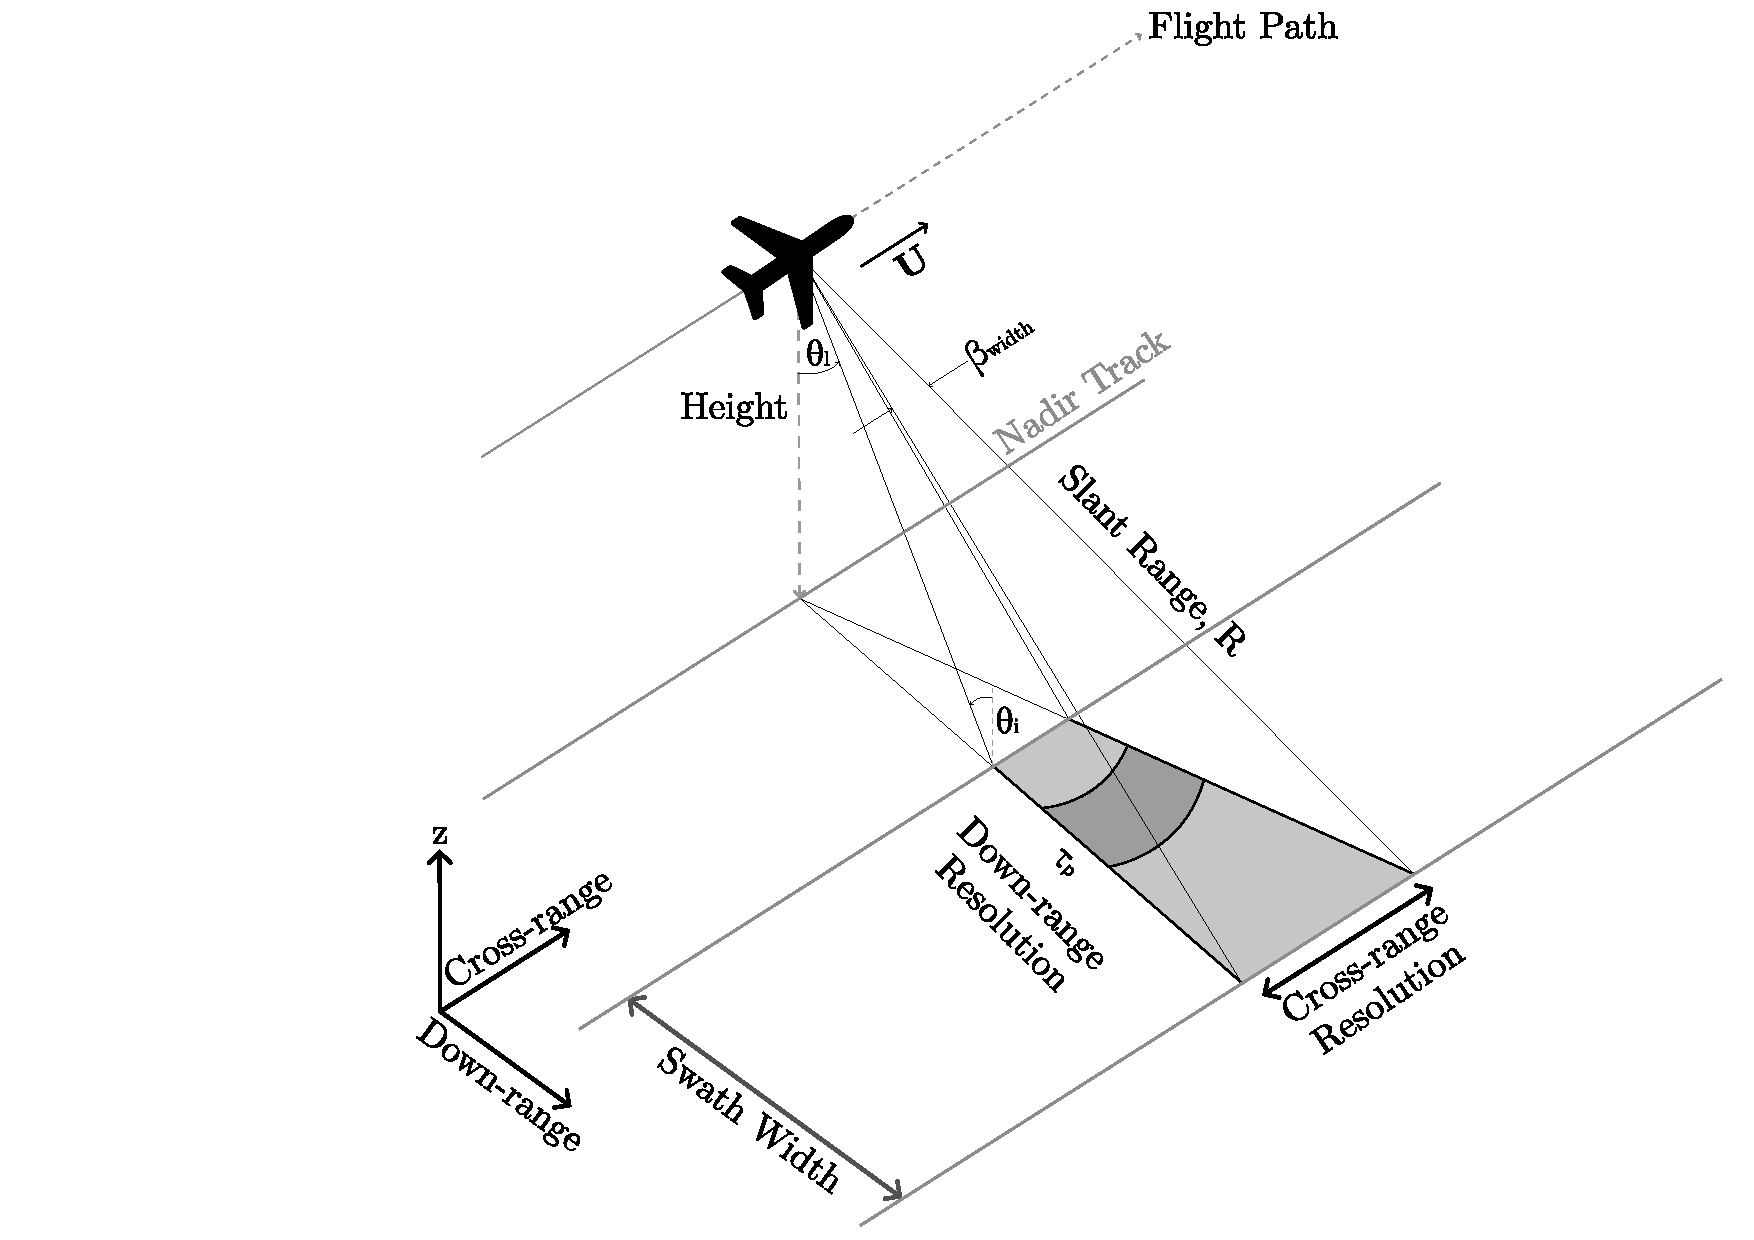
\includegraphics[width=.95\linewidth]{Figures/Theory/slarGeometry.pdf}
    \caption{Graphical representation of a \acs{slar} system with important features labelled. Adapted from \cite{Moreira2013,Meyer2019}.}
    \label{fig:theory.slarGeometry}
\end{figure}

The radar system operates by transmitting a series of chirps, each with a pulse length defined as $\tau_{p}$, which illuminate the region of the ground referred to as the antenna footprint \cite{Meyer2019}. To calculate the size of this footprint, consider the radar's slant range, $R$, which represents the distance between the antenna and its footprint, as well as the beamwidth, denoted as $\beta_{width}$. The beamwidth can be defined as the ratio between the radar's wavelength, $\lambda$, and the antenna length, $L_{ant}$. This definition enables the determination of the antenna footprint size, $S$ \cite{Meyer2019}

\begin{equation} \label{eq:rar.footprintSize}
    S \approx \frac{\lambda}{L_{ant}}R = \beta_{width} R \,\, \text{[m]}
\end{equation}

This footprint is shown in dark grey in Figure \ref{fig:theory.slarGeometry} as well as depicting the incidence angle, $\theta_{i}$, which can be derived as $90 \degree - \theta_{l}$. The resolution of this beamwidth in both the down-range and cross-range directions can be empirically determined. The slant range resolution of a \ac{slar} system is defined in terms of the speed of light, $c$ and the pulse length, $\tau_{p}$ as

\begin{equation} \label{eq:rar.slantRangeResolution}
    \delta_{sr} = \frac{c \tau_{p}}{2} \,\, \text{[m]}
\end{equation}

The resolution of a radar system allows it to differentiate between different objects at different slant ranges from the sensor \cite{Moreira2013}. It is also useful to define the down-range resolution in terms of the incidence angle and slant range resolution as

\begin{equation} \label{eq:rar.groundRangeResolution}
    \delta_{dr} = \frac{\delta_{sr}}{\text{sin}(\theta_{i})} \,\, \text{[m]}
\end{equation}

and the cross-range resolution as

\begin{equation} \label{eq:rar.crossrangeResolution}
  \delta_{cr} = \frac{\lambda}{L_{ant}}R \,\, \text{[m].}
\end{equation}

In order to see the drawback of \ac{rar} in terms of resolution, it is useful to apply values to Equation \ref{eq:rar.crossrangeResolution}. Consider an X-band\footnote{Give wavelength and freq of X-band} \ac{rar} radar system with a slant range to the target of 7\,km, as in a space-borne application, and with an antenna length of 5\,m. This yields a cross-range resolution of

\begin{gather*}
    \delta_{cr} = \frac{0.03\,\text{m}}{5\,\text{m}} \cdot 7000\,\text{m} = 42\,\text{m}
\end{gather*}

The above example shows that a space-borne application of \acs{rar} results in a loss of cross-range resolution. In the context of this project, this is impractical as ocean waves need to be imaged and differentiated between.

The limited resolution of \acs{rar} led to the development of \acs{sar}. This technology addresses the impact of antenna length by synthetically imitating a longer antenna length, which enhances the cross-range resolution. This is accomplished through exploiting the Doppler shift phenomenon and capturing multiple images of the same scene. For a more comprehensive understanding of the mathematical and signal processing aspects involved in generating a \acs{sar}, refer to \cite{Cumming2005}.


The synthetic length of the antenna \cite{Meyer2019} used in calculating the cross-range resolution can be determined as

\begin{equation} \label{eq:sar.virtualAntennaL}
    L_{SA} \approx \beta_{width}\cdot R 
\end{equation}

where the artificial beamwidth can be calculated as

\begin{equation} \label{eq:sar.beamwidth}
    \beta_{witdth_{SA}} = \frac{\lambda}{2L_{SA}}
\end{equation}

This, in turn, allows the cross-range resolution \cite{Moreira2013} for a \acs{sar} sensor to be calculated as

\begin{equation} \label{eq:sar.crossRangeResolution}
    \delta_{cr_{SA}} = R\cdot \beta_{SA} = R \cdot \frac{\lambda}{2L_{SA}} = \frac{L_{ant}}{2}
\end{equation}

Using the previous example of a space-borne sensor with an antenna of length, 5\,m, it can be seen that \acs{sar} improves the cross-range resolution when compared to \acs{rar}.

\begin{gather*}
    \delta_{cr_{SA}} = \frac{5\,\text{m}}{2} = 2.5\,\text{m}
\end{gather*}

This example shows that \acs{sar} allows fine cross-range resolution, a vital parameter in the application of imaging ocean waves. Along with this, \acs{sar} offers year-round imaging in any weather conditions as discussed in Section \ref{sec:litReview.sarCharac}.
% Check section ref

\subsection{\acs{sar} Imaging Modes} \label{subsec:theory.sar.imaging}
% SAR Imaging

Each \acs{sar} sensor can capture data in multiple modes with the most common modes being Spotlight, \ac{sm}, and ScanSAR. Sentinel-1A offers data products using three main capture modes: \acs{sm}, \ac{iw}, and \ac{ew} modes. \ac{iw} and \ac{ew} are both a new type of Scan\acs{sar} based on \ac{topsar}. These capture modes are shown visually in Figure \ref{fig:theory.sarCaptureModes} where $U$ represents the satellite's velocity.

%TOPS ref \cite{Huang2014}.


\begin{figure} [H]
    \centering
    \begin{subfigure}{0.48\textwidth}
        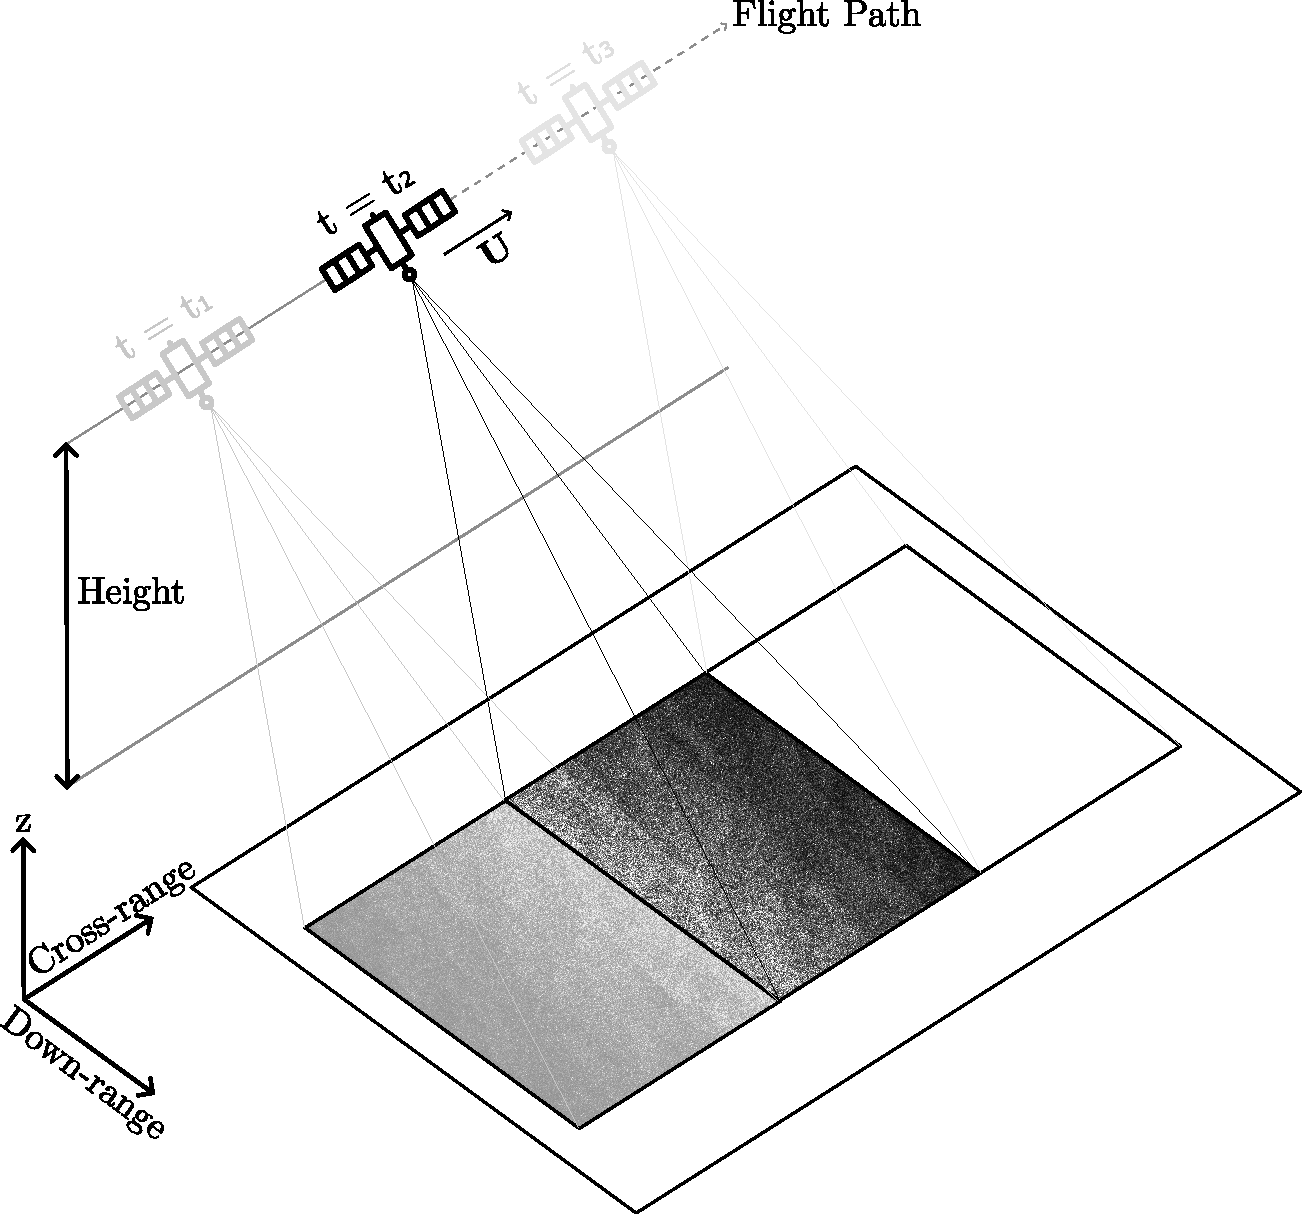
\includegraphics[width=\textwidth]{Figures/Theory/stripmap.pdf}
        \caption{\acf{sm} capture mode.}
        \label{fig:theory.stripmap}
    \end{subfigure}   
    \begin{subfigure}{0.48\textwidth}
        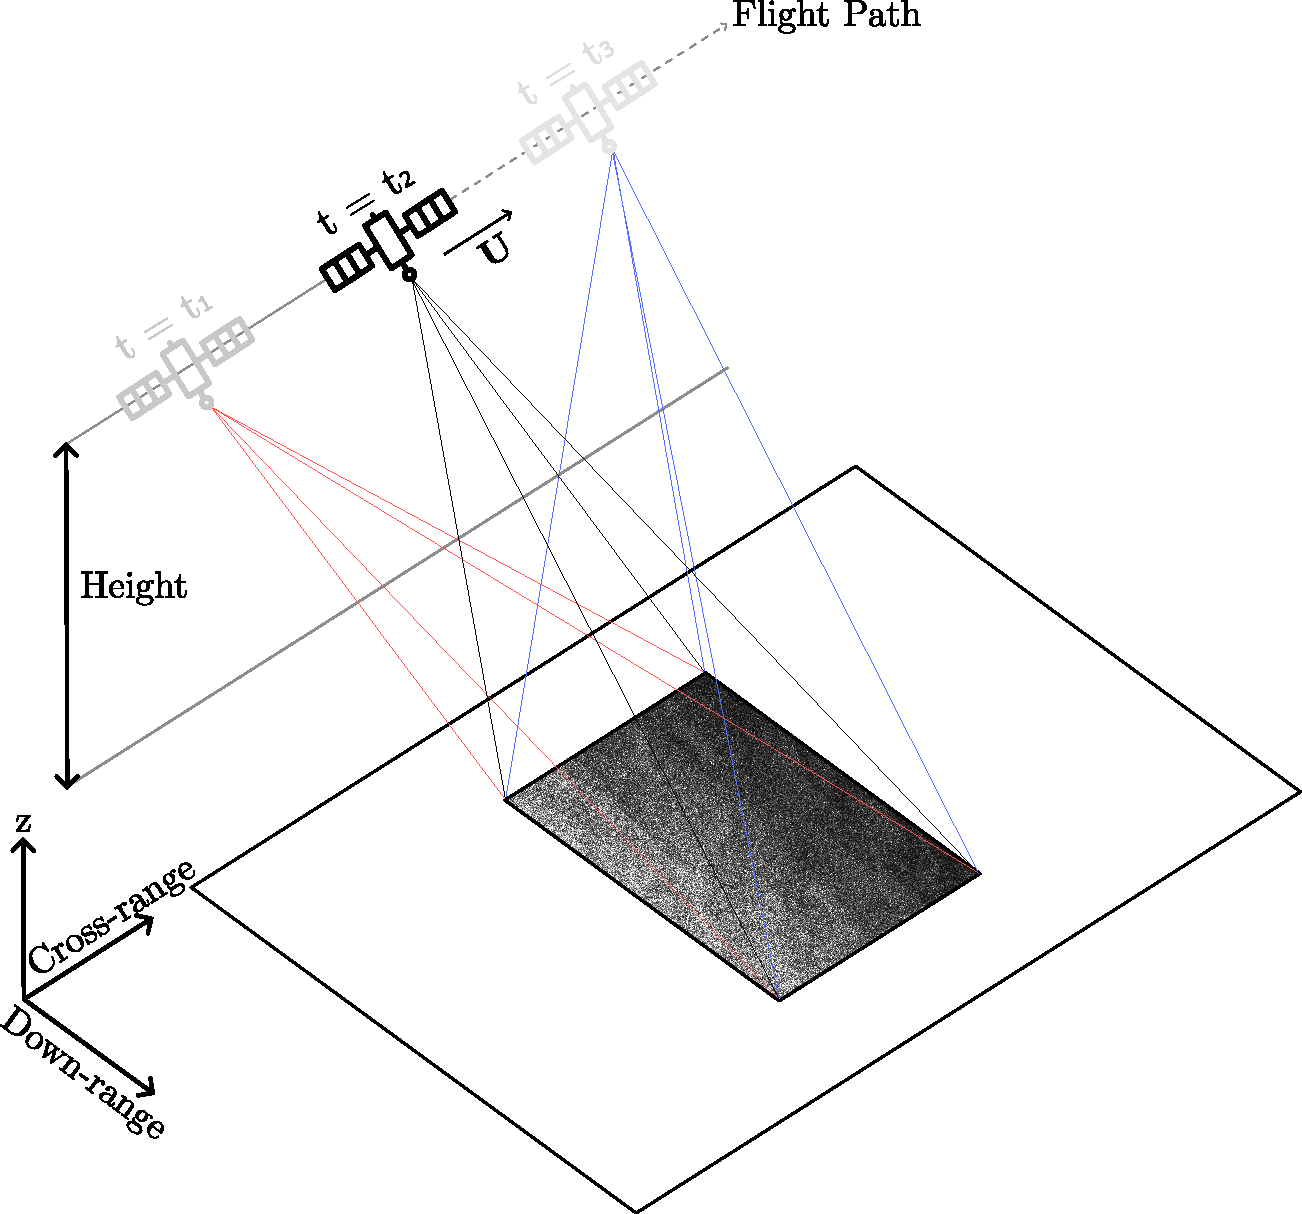
\includegraphics[width=\textwidth]{Figures/Theory/spotlight.pdf}
        \caption{Spotlight capture mode.}
        \label{fig:theory.spotlight}
    \end{subfigure} 
    \begin{subfigure}{0.48\textwidth}
        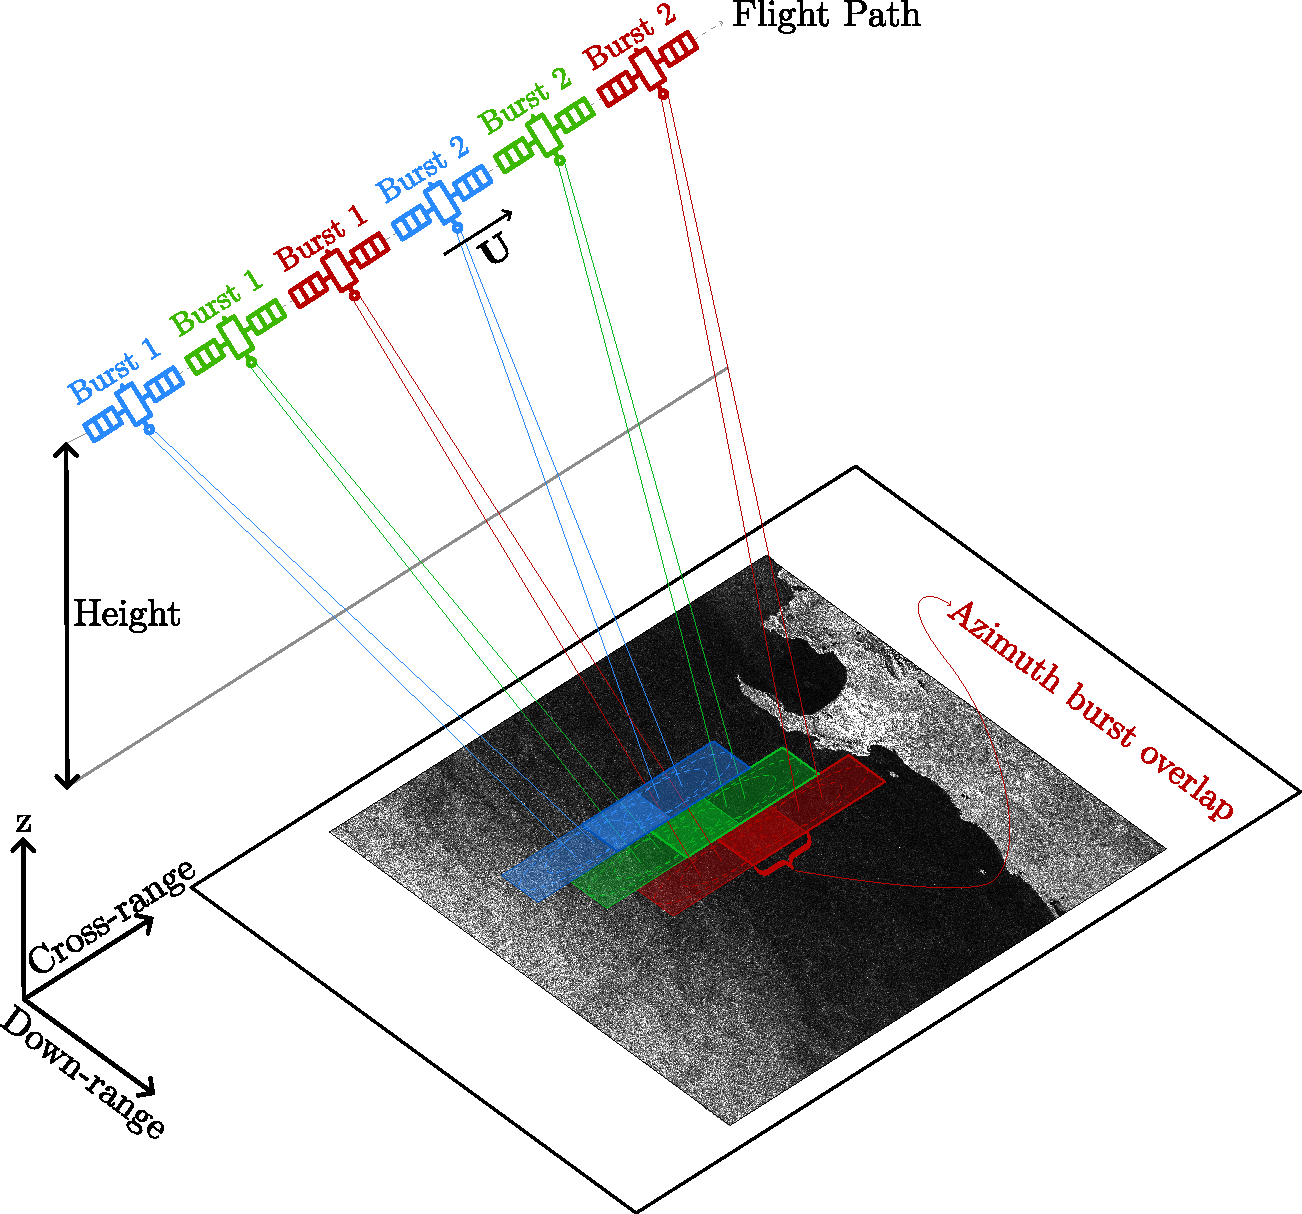
\includegraphics[width=\textwidth]{Figures/Theory/scanSAR.pdf}
        \caption{Scan\acs{sar} capture mode.}
        \label{fig:theory.scanSAR}
    \end{subfigure} 
    \begin{subfigure}{0.48\textwidth}
        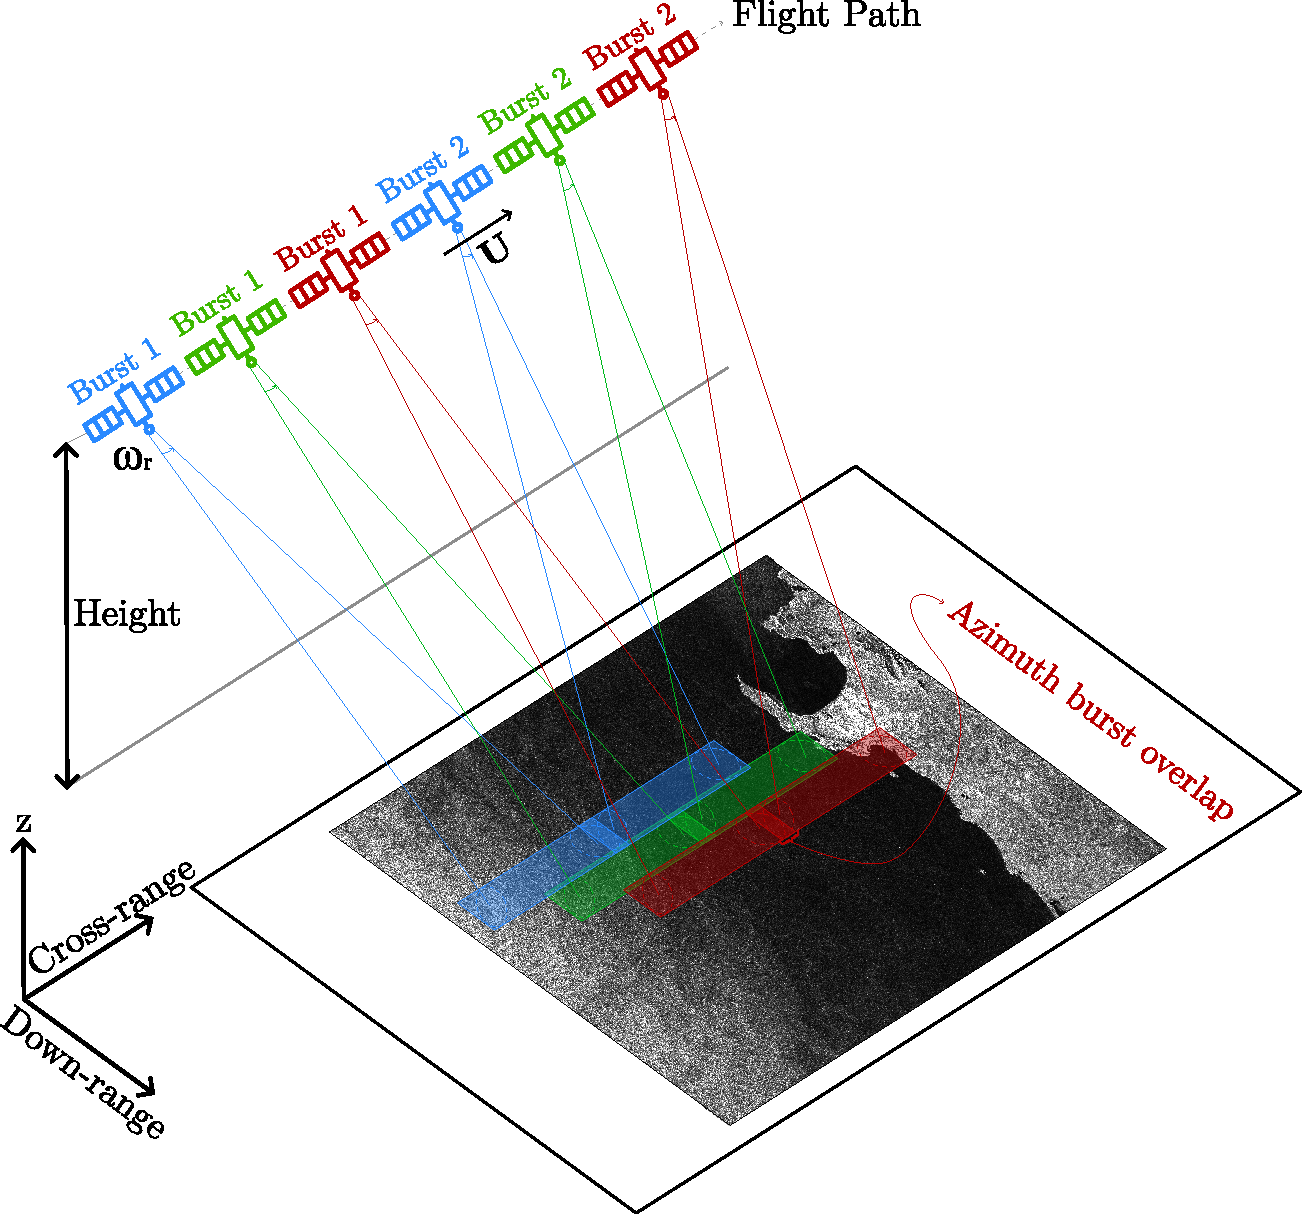
\includegraphics[width=\textwidth]{Figures/Theory/tops.pdf}
        \caption{\acs{topsar} capture mode used by \acs{s1a}. Adapted from \cite{Huang2014}.}
        \label{fig:theory.tops}
    \end{subfigure}     
    \caption{Graphical representation of commonly used \acs{sar} satellite capture and specific \acs{s1a} capture modes.}
    \label{fig:theory.sarCaptureModes}
\end{figure}

 % fix spelling and grammar of all

\subsubsection{\acf{sm} Mode}

\acs{sm} mode is the conventional \acs{sar} imaging mode \cite{Frery2022}. In \acs{sm} mode, the antenna has a fixed direction, which observes a fixed swath, whilst the satellite moves along its flight path \cite{Moreira2013} as depicted in Figure \ref{fig:theory.stripmap}. This allows a continuous ground swath to be illuminated with a continuous sequence of chirps. The echoes received back by the sensor are processed and combined to form a continuous image of the observed scene. \acs{sm} mode provides increased cross-range resolution as multiple echoes are received back from the same target within the scene. \acs{sm} mode is a versatile imaging mode as it allows detailed imagery over a large area to be obtained over a single, continuous strip at a constant incidence angle \cite{Moreira2013,Frery2022,sentinel1ProductDef}.


% \acs{sm} mode, is the conventional \acs{sar} imaging mode \cite{Frery2022}, and features a fixed antenna direction observing a constant swath while the satellite progresses along its flight path, as shown in Figure \ref{fig:theory.stripmap}. This mode enables continuous ground swath illumination via a sequence of chirps, leading to a continuous scene image. It offers enhanced cross-range resolution due to multiple echoes from the same target, making it versatile for detailed imaging over a large area at a consistent incidence angle \cite{Moreira2013, Frery2022, sentinel1ProductDef}.

\subsubsection{Spotlight Mode}

Spotlight mode is used for high-resolution \acs{sar} imaging \cite{Meyer2019}, and involves targeting a specific area while continuously illuminating and capturing echoes during satellite movement along its flight path, as depicted in Figure \ref{fig:theory.spotlight}. Antenna beam control can be achieved mechanically or electronically through beam steering \cite{Frery2022}. Spotlight mode improves both down- and cross-range resolutions. Whilst its spatial coverage is smaller compared to \acs{sm} mode. By extending the synthetic antenna's length, Spotlight mode enhances cross-range resolution, making it ideal for applications requiring maximum resolution whilst accepting reduced spatial coverage \cite{Moreira2013}.

% Spotlight mode is recommended for high-resolution \acs{sar} imaging \cite{Meyer2019}. In Spotlight mode, the radar antenna targets a specific area whilst continuously illuminating this area and capturing the received echoes whilst travelling along its flight path \cite{Frery2022,Moreira2013}, as depicted in Figure \ref{fig:theory.spotlight}. The antenna beam is controlled either mechanically, or electronically through beam steering \cite{Frery2022} to ensure that the desired target is continuously illuminated over the capture time as the satellite travels along its flight path. Spotlight mode enhances both the down- and cross-range resolutions. Whilst Spotlight mode has a smaller spatial coverage than \acs{sm} mode, it trades this off for increased resolution. Spotlight mode increases the cross-range resolution by increasing the length of the synthetic antenna and it is useful when maximum resolution is required for an application with decreased spatial coverage \cite{Moreira2013}.

\subsubsection{Scan\acs{sar} Mode}

Scan\acs{sar} mode provides improved spatial coverage compared to both \acs{sm} and Spotlight modes, although at the cost of reduced cross-range resolution \cite{Frery2022}. In Scan\acs{sar}, the antenna periodically sweeps over multiple sub-swaths associated with various antenna orientations \cite{Frery2022,Moreira2013}, as shown in Figure \ref{fig:theory.scanSAR}. Each sub-swath is illuminated by multiple chirps but for a shorter duration compared to \acs{sm} mode \cite{Moreira2013}. The loss in resolution is due to the fact that the synthetic antenna length is divided up across the sub-swaths \cite{Frery2022}.

% Scan\acs{sar} mode offers increased spatial coverage, through the increase in swath width, over both \acs{sm} and Spotlight mode at the cost of reduced cross-range resolution \cite{Frery2022}. Scan\acs{sar} mode operates by having the antenna periodically sweep over various sub-swaths associated with various antenna orientations \cite{Frery2022,Moreira2013}, as depicted in Figure \ref{fig:theory.scanSAR}. Each sub-swath is illuminated by multiple chirps, but for a shorter time than in \acs{sm} mode \cite{Moreira2013} and the antenna orientation is changed by varying the look angle, $\theta_{l}$ of the antenna. These sub-swaths are combined when processing the raw data and result in increased swath width, with decreased cross-range resolution when compared to \acs{sm} and Spotlight modes \cite{Moreira2013}. This loss in resolution is due to the fact that the synthetic antenna length is divided up across the sub-swaths \cite{Frery2022}.

\subsubsection{\acs{topsar} Mode}

\ac{topsar} is a specialised form of Scan\acs{sar} imaging used by \acs{s1a} in both \ac{iw} and \ac{ew} modes. It acquires data by transmitting bursts and periodically switching the antenna beam between adjacent sub-swaths, as illustrated in Figure \ref{fig:theory.tops}. While Scan\acs{sar} uses mechanical or electronic beam steering, \acs{topsar} exclusively uses electronic beam steering in both down- and cross-range directions. \acs{topsar} offers the same spatial coverage as Scan\acs{sar} but with marginally improved cross-range resolution due to shorter burst times \cite{DeZan2006}. Consequently, \acs{topsar} is ideal for applications demanding high resolution and extensive swath coverage.

\acs{s1a}'s \acs{iw} mode uses \acs{topsar} imaging, retaining wide swath coverage and improved cross-range resolution \cite{sentinel1ProductDef}. \acs{iw} mode consists of three wide sub-swaths captured by steering the antenna in the cross-range direction by an angle $\omega_{r}$ \cite{sentinel1ProductDef}. On the other hand, \acs{ew} mode, also based on \acs{topsar} imaging, differs in the number of sub-swaths used for complete scene capture. While \acs{iw} mode utilises three sub-swaths, \acs{ew} mode employs five wide sub-swaths to construct the entire image, effectively enhancing spatial coverage while maintaining cross-range resolution.

% \ac{topsar} is a specialised form of Scan\acs{sar} imaging used by \acs{s1a} in both \ac{iw} and \ac{ew} modes. \acs{topsar} captures data by transmitting bursts whilst periodically switching the antenna beam between adjacent sub-swaths \cite{DeZan2006}, as depicted in Figure \ref{fig:theory.tops}. Whilst Scan\acs{sar} uses mechanical or electronic beam steering, \acs{topsar} utilises only electronic beam steering and does this in both the down- and cross-range directions. \acs{topsar} offers the same spatial coverage as Scan\acs{sar}, whilst marginally improving cross-range resolution due to shorter burst times when compared to Scan\acs{sar} \cite{DeZan2006}. Thus, \acs{topsar} is useful for high-resolution and large swath applications. 

% \acs{iw} mode implemented by \acs{s1a} utilises \acs{topsar} imaging and maintains the wide swath coverage and improved cross-range resolution \cite{sentinel1ProductDef}. \acs{iw} captures are made up of three wide sub-swaths \cite{sentinel1ProductDef} captured by beam steering the antenna in the cross-range direction through an angle, $\omega_{r}$. \ac{ew} mode is also based on \acs{topsar} imaging techniques and differs from \acs{iw} mode in the number of sub-swaths which are used when capturing the full scene. Where \acs{iw} mode uses three sub-swaths, \acs{ew} mode utilises five wide sub-swaths to construct the full image whilst maintaining cross-range resolution and increasing the spatial coverage of the capture.

Table \ref{tab:theory.s1aImagingParams} provides a comparison of the ground resolution of all \acs{s1a} imaging techniques for \acs{grd} data.

\begin{table}[H]
\centering
\begin{tabular}{|c|c|c|}
\hline
\textbf{Mode} & \multicolumn{1}{l|}{\textbf{Minimum Ground Swath Width {[}km{]}}} & \multicolumn{1}{l|}{\textbf{Resolution (dr x cr) {[}m{]}}} \\ \hline
\textbf{\acs{sm}} & 80 & 10x10 \\ \hline
\textbf{\acs{iw}} & 250 & 10x10 \\ \hline
\textbf{\acs{ew}} & 410 & 25x25 \\ \hline
\end{tabular}
\caption{Comparison of ground swath width and resolution of \acs{s1a} imaging modes. Adapted from \cite{sentinel1ProductDef}}
\label{tab:theory.s1aImagingParams}
\end{table}

Due to the fact that this project requires imaging ocean waves, fine-range resolution is required. To this end, data products captured using \acs{sm} or \acs{iw} mode are utilised due to their improved resolution over \acs{ew} mode depicted in Table \ref{tab:theory.s1aImagingParams}.




% \subsubsection{Data Levels}

% \begin{itemize}
%     \item Data levels (Level 0 - I and Q, Level 1 - GND)
% \end{itemize}

\subsection{Pre-processing Techniques} \label{subsec:theory.sar.preProcess}

\textbf{Speckle}

Speckle, often noted for its "salt-and-pepper" appearance \cite{Meyer2019} in \acs{sar} images, results from the interference of multiple scatters within a resolution cell which leads to varying intensity values. Even when imaging a uniform surface, speckle exists due to phase variations amongst scatterers within the resolution cell, with brighter image regions exhibiting more intense speckle \cite{Moreira2013,Meyer2019}. Speckle is not an error in a \acs{sar} image, but a consequence of imaging with finite resolution. Higher resolution weakens the speckle effect as it reduces the number of scatterers within the resolution cell \cite{Meyer2019}. Unprocessed intensity VV \acs{grd} data is shown in Figure \ref{fig:theory.data.unprocessed} and speckle can be seen in both sub-scenes.

\begin{figure}[H]
    \centering
    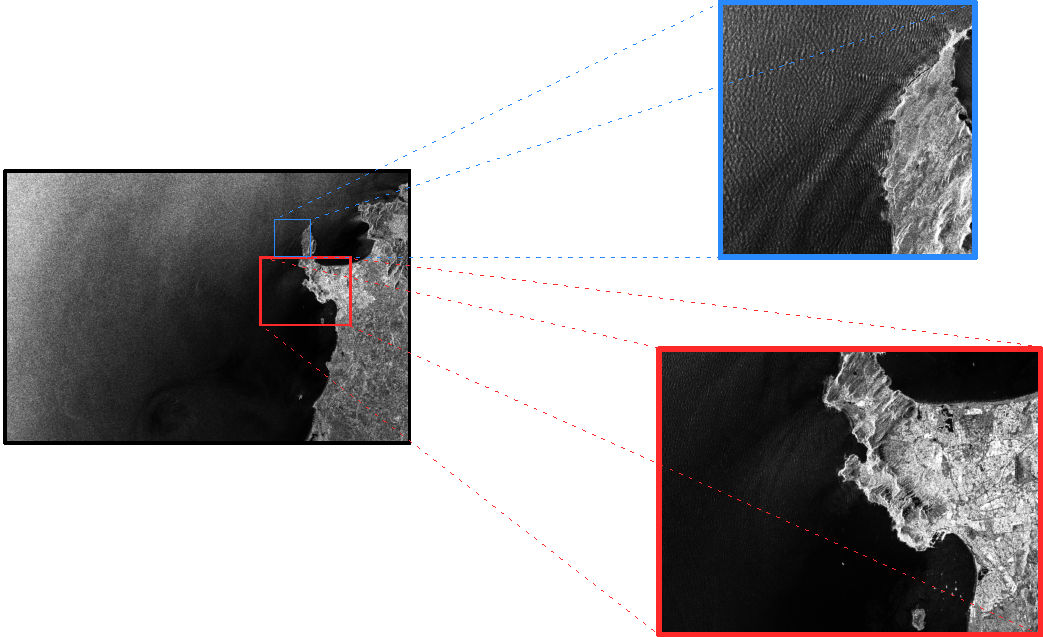
\includegraphics[width=0.85\textwidth]{Figures/Theory/unprocessedSARData.pdf}
    \caption{Unprocessed \acs{grd} \acs{s1a} data.}
    \label{fig:theory.data.unprocessed}
\end{figure}

\textbf{Thermal Noise}
% Check spelling and grammar

Thermal noise significantly affects \acs{sar} image quality. It represents inherent background energy generated by the radar receiver channel and creates a noise threshold. When a received signal falls below this threshold, it becomes indistinguishable from thermal noise, which impacts low-intensity scatterers, such as new ice and open water \cite{Carsey1992}, especially in cross-polarised applications. In these cases, the thermal noise can significantly impact the interpretability of the \acs{sar} data \cite{Carsey1992}. Unlike speckle, which appears as grainy patterns and can be reduced through filtering, thermal noise is characterised by a uniform background noise level. In the context of \acs{s1a}, thermal noise is composed of two additive noise sources related to antenna movement and scalloping noise\footnote{Define scalloping noise}. It predominantly affects \acs{topsar} imaging mode, especially for cross-polarised images.

% Thermal noise is a significant factor in \acs{sar} imaging as it influences the quality of these images. Thermal noise represents the inherent background energy generated by the radar receiver channel \cite{Park2018}. Thermal noise is responsible for creating a noise threshold for a \acs{sar} image. When a received signal drops below this noise threshold, it becomes nearly indistinguishable from the thermal noise. This poses an issue for analysing scatterers which return low-intensity values, such as new ice and open water \cite{Carsey1992}. In these cases, the thermal noise can significantly impact the interpretability of the \acs{sar} data \cite{Carsey1992}.

% While speckle noise appears as grainy patterns across the image and can often be reduced by filtering techniques \cite{Meyer2019}, thermal noise is characterized by a uniform, background noise level. Speckle noise is a result of the coherent nature of \acs{sar} imaging, leading to constructive and destructive interference of radar signals. Thermal noise, on the other hand, results from the receiver's inherent noise and significantly impacts low backscatter targets, especially in cross-polarised channels \cite{Park2018,Park2019}.

% In the context of \acs{s1a}, thermal noise plays an important role. Thermal noise is comprised of two sources of additive noise. The first is linked to the movement of the antenna and causes variability in the down-range direction. The second is known as scalloping noise\footnote{define scalloping noise} and varies in the cross-range direction \cite{Park2019}. Thermal noise impacts \acs{topsar} imaging mode more than others, particularly for cross-polarised images \cite{Park2018}. Furthermore, \acs{s1a} \acs{ew} mode \acs{sar} images, particularly those acquired over regions with a low backscatter, such as calm oceans and young smooth sea ice, are susceptible to thermal noise \cite{Carsey1992}.

Removal of \acs{s1a} thermal noise results in improved image quality and can be visually seen in Figure \ref{fig:theory.data.thermalNoiseRemoval} when compared to Figure \ref{fig:theory.data.unprocessed}, particularly over land regions in the second sub-scene.

\begin{figure}[H]
    \centering
    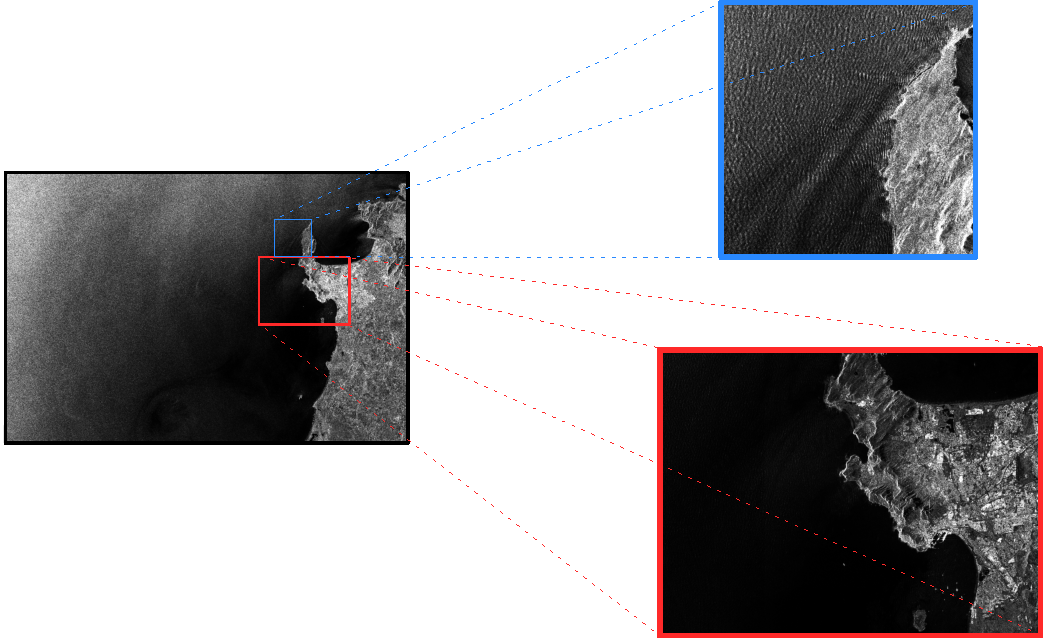
\includegraphics[width=0.85\textwidth]{Figures/Theory/thermalNoiseCalibratedSARData.pdf}
    \caption{\acs{grd} \acs{s1a} data with thermal noise removed using \acs{snap}.}
    \label{fig:theory.data.thermalNoiseRemoval}
\end{figure}

\subsubsection{Radiometric Calibration}
% Reword

In \acs{sar} imaging, $\sigma_{0}$ represents the backscatter coefficient, which indicates the radar signal's strength reflected by scatterers. $\sigma_{0}$ is a dimensionless number that accounts for variations in factors like incidence angle, wavelength, polarisation, and surface properties. Radiometric calibration addresses \ac{rcs} variations, ensuring that pixel values in \acs{sar} images are both qualitatively representative and quantitatively aligned with $\sigma_{0}$. This process corrects radiometric bias present in raw \acs{sar} data, enabling its use in quantitative applications like target recognition and environmental monitoring. Calibration factors in the scattering area, antenna gain pattern, and range spread loss, enhance the accuracy and reliability of \acs{sar} data.

% Fact check
Radiometric calibration of \acs{s1a} \acs{grd} data can be visually seen in Figure \ref{fig:theory.data.radiometric} over mountainous regions in both sub-scenes. This is due to the correction of backscatter bias which doesn't account for elevation changes.

% In \acs{sar} imaging, $\sigma_{0}$ is known as the backscatter coefficient and acts as an indicator of the strength of radar signals reflected by scatterers. It provides a normalised dimensionless number that allows for comparing the observed signal strength to what would be expected from a standard one-square-meter area \cite{ElDarymli2014}. It's important to emphasise that $\sigma_{0}$ exhibits significant variations based on factors such as incidence angle, wavelength, polarisation, and the properties of the scattering surface itself. 

% Radiometric calibration in SAR images is a vital process, and it primarily involves addressing the variations in \acs{rcs}, which quantifies the radar signal's strength reflected by distributed scatterers. Calibration ensures that pixel values in \acs{sar} images are not only qualitatively representative but also quantitatively aligned with the \acs{rcs} and backscatter coefficient, $\sigma_{0}$. Essentially, radiometric calibration rectifies the radiometric bias present in the raw \acs{sar} data, making it suitable for a wide array of quantitative applications. This calibration process includes adjustments for factors like scattering area, antenna gain pattern, and range spread loss, guaranteeing the accuracy and reliability of \acs{sar} data for applications such as target recognition and environmental monitoring.

% Update calibrated image
\begin{figure}[H]
    \centering
    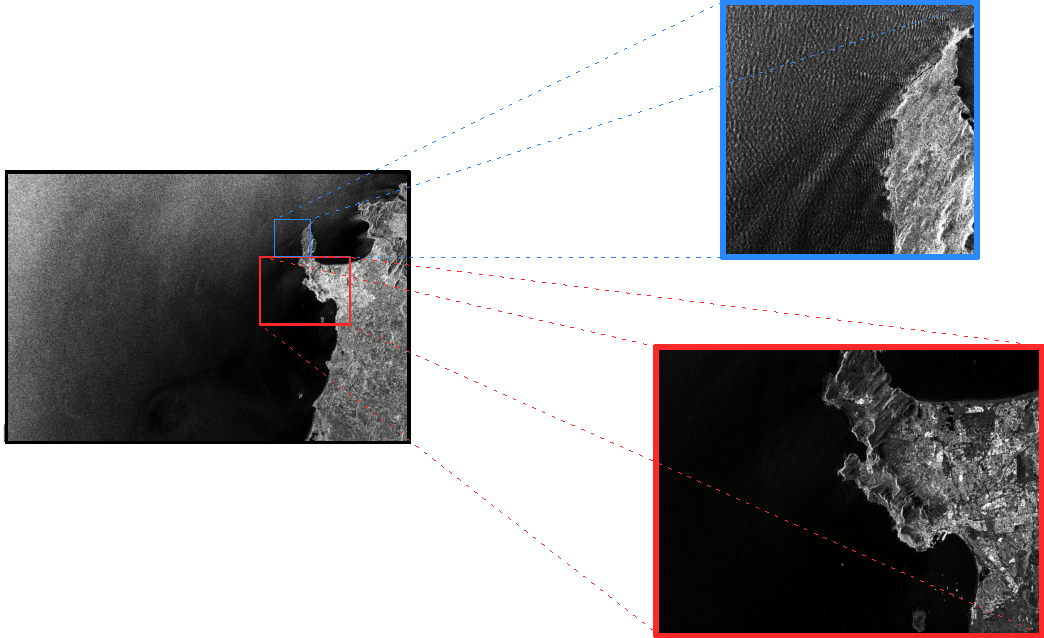
\includegraphics[width=0.85\textwidth]{Figures/Theory/radiometricCalibratedSARData.pdf}
    \caption{Radiometrically calibrated \acs{grd} \acs{s1a} data done using \acs{snap}.}
    \label{fig:theory.data.radiometric}
\end{figure}

\begin{itemize}
    \item Mention geocoding and terrain rectification (Link why this is the case)
    \item Speak about speckle (or link)
    \item Thermal Noise Removal
    \item Radiometric calibration
    \item Show graphically what each technique does and how it changes the image (Maybe in the appendix)
\end{itemize}

\subsection{Polarisation} \label{subsec:theory.sar.polarisation}

Polarisation is a fundamental aspect of \acs{sar} imaging. Polarisation refers to the orientation of the plane in which an \acs{em} wave oscillates as it propagates. Linear polarisation maintains a constant orientation along the wave's path, while circular and elliptical polarisations involve changing oscillation plane orientations, forming shapes like ellipses or circles \cite{Meyer2019}.

Traditionally, most \acs{sar} systems used single-polarised sensors, predominantly operating in HH (horizontal transmit, horizontal receive) or VV (vertical transmit, vertical receive) polarisation. However, newer \acs{sar} sensors offer dual-polarisation or quad-polarisation capabilities. These sensors can transmit both horizontally and vertically polarised waveforms and receive signals from both polarisations. Understanding the polarisation of a \acs{sar} image is crucial as it affects how radar signals interact with objects on the ground, influencing the recorded radar brightness for specific polarisations.

To interpret polarimetric SAR data effectively, it is helpful to consider how different types of scatterers interact with different polarizations. Rough surface scatterers, double-bounce scatterers, and volume scatterers make up the three primary categories of scatterers in a scene. Different polarimetric channels exhibit varying preferences for these scattering types, and these preferences can be used to analyse and classify scattering types. 


\subsubsection{Scattering}

Scattering is important to understand how satellite sensors detect and interpret \acs{em} waves. Scattering on the Earth's surface involves two primary processes: surface and volume scattering. Surface roughness plays a critical role in \acs{em} backscatter. A flat or specular surface\footnote{Define specular surface} behaves like a mirror, reflecting radiation back to the sensor only when the surface aligns perpendicularly with the sensor's line of sight. This occurs with flat or tilted surfaces, such as mountains or ocean surface waves. In contrast, rougher surfaces scatter a portion of incident EM radiation back toward the sensor. 

When the surface has a regular structure, such as waves with a specific wavelength, it can result in positive interference, a phenomenon known as Bragg scattering. Bragg scattering is of particular interest in the context of ocean waves and is caused by short ripple waves on the ocean surface \cite{Hasselmann1991}. This phenomenon is characterised by the constructive interference of incoming and backscattered \acs{em} radiation due to the regular structure of waves. This creates high backscatter values. The key factor for Bragg scattering's occurrence is the consistency between the wavelength of the electromagnetic waves and the spacing between wave crests.

% Bragg scattering enables radar instruments like scatterometers and Synthetic Aperture Radar (SAR) sensors to capture information about surface waves on the ocean, aiding in various applications like wave height and wind speed retrieval. 

%This effect is especially prominent at microwave frequencies, where ripple waves on water have wavelengths on the order of the EM wavelength. 



\begin{figure} [H]
    \centering
    \begin{subfigure}{0.31\textwidth}
        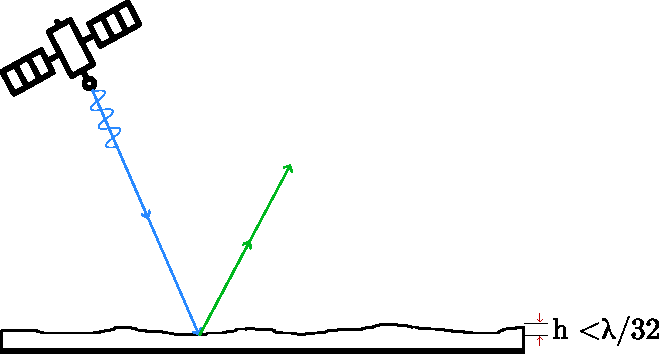
\includegraphics[width=\textwidth]{Figures/Theory/smoothSurface.pdf}
        \caption{\textbf{Smooth surface} \\ Near-perfect specular reflection.}
        \label{fig:theory.data.surface.smooth}
    \end{subfigure}   
    \begin{subfigure}{0.35\textwidth}
        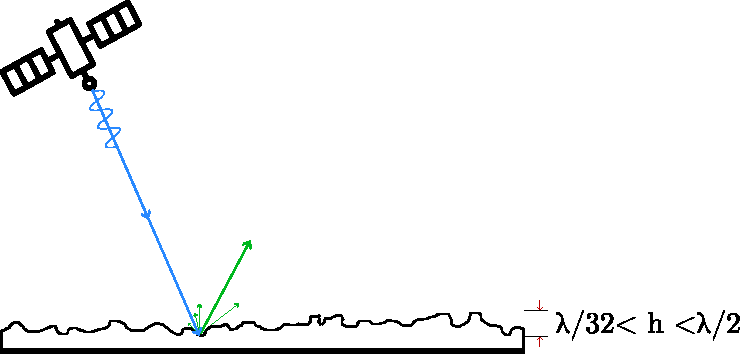
\includegraphics[width=\textwidth]{Figures/Theory/intermediateSurface.pdf}
        \caption{\textbf{Intermediate surface} \\ Moderate signal return.}
        \label{fig:theory.data.surface.intermediate}
    \end{subfigure} 
    \begin{subfigure}{0.31\textwidth}
        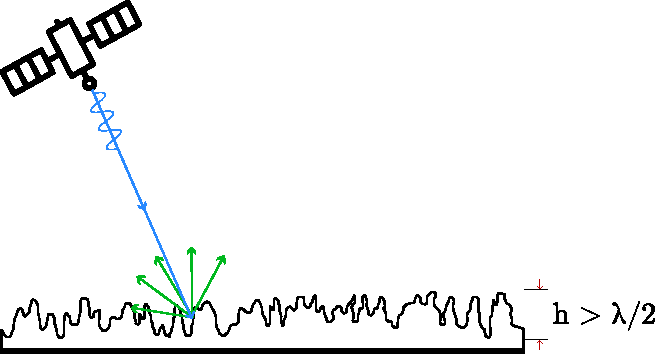
\includegraphics[width=\textwidth]{Figures/Theory/roughSurface.pdf}
        \caption{\textbf{Rough surface} \\ Diffuse scattering.}
        \label{fig:theory.data.suface.diffuse}
    \end{subfigure}    
    \caption{Comparison of surface roughness and surface backscatter. Adapted from \cite{Meyer2019}.}
    \label{fig:theory.data.surface}
\end{figure}

% Scatterers, surface roughness and penetration of wavelength (NEEED NEW TITLE)
% Speckle - Page 918 of PoMR
%   - Page 148 of Radar Imaging of Ocean Waves
\begin{itemize}
    \item Penetration of radar signals (Link to wavelength)
    \item - In the context of this work (Ocean waves [bragg scattering of wind-generated ripple waves] and sea ice)
    \item Surface roughness
    \item Scattering types
\end{itemize}

\begin{itemize}
    \item Speak about different polarisations and why each is good at what it does (In wave, ocean and land context)
    \item Visually show how each differs
    \item Focus on VV and HH and why they are used for Hasselmann in the context of ocean waves
\end{itemize}

%====================================================
% SAR OCEAN WAVE INVERSION
%====================================================
% \section{\acs{sar} Ocean Wave Inversion} \label{sec:theory.oceanWaveInversion}
% % Explain link to sea ice and wave modelling
% \subsection{Hasselmann and Hasselmann Inversion Technique} \label{subsec:theory.oceanWaveInversion.Hasselmann}
\section{Hasselmann and Hasselmann Ocean Wave Inversion Technique} \label{sec:theory.hasselmann}
The \ac{hh} process maps an ocean wave spectrum, as described in Section \ref{sec:theory.waves}, into a \ac{sar} image spectrum, as described in Section \ref{sec:theory.sar}. The \ac{hh} inversion procedure consists of two main parts - the \acs{sar} imaging of ocean waves, followed by an inversion to extract a wave spectrum. A full derivation of the \ac{hh} procedure is given in Appendix \ref{ap:hh}, however, an overview of the procedure, along with the relevant formulas is given in the following section.

%\subsubsection{\acs{sar} Imaging of Ocean Waves} \label{subsubsec:theory.oceanWaveInversion.Hasselmann.sarImaging}
\subsection{\acs{sar} Imaging of Ocean Waves} \label{subsec:theory.hasselmann.sarImaging}

\acs{hh} \cite{Hasselmann1991} state that the waves captured by a \acs{sar} spectrum are modulated through three different modulation processes. Firstly, the change in incidence angle is due to the change in the slope of the wave face. Secondly, the interactions between short and long waves, which modulate the energy and wave number of the short, Bragg scattering, ripple waves. And thirdly, the orbital velocity of the long waves, which produces a Doppler shift in the received, return signal. This causes an azimuthal displacement of the scatterers in the \acs{sar} image. This third modulation process is known as velocity bunching and is the main cause of nonlinearity in the imaging of ocean waves. All three of these modulation processes can be represented by their respective modulation transfer functions, and are denoted by the general form, $T^x_k$.

In order to derive a \acs{sar} spectrum from an ocean wave spectrum, \acs{hh} treat the captured \acs{sar} image as two separate procedures, namely the frozen surface, defined by the \ac{rar} imaging mechanism, and the motion effects, related to \acs{sar} imaging. The reason these motion effects arise is due to the way in which a \acs{sar} image is captured, as discussed in Section \ref{subsec:theory.sar.imaging}.

\subsubsection{Frozen Surface Contribution} \label{subsubsec:theory.hasselmann.sarImaging.frozenSurface}

%\textit{\textbf{Frozen Surface Contribution}}

The \ac{rar} \ac{mtf} \cite{Hasselmann1991} can be defined as 

\begin{equation} \label{eq:hh.rar.TR_k_sum}
    T^R_k = T^t_k + T^h_k
\end{equation}

where $T^t_k$ and $T^h_k$ are the tilt and hydrodynamic interaction \acp{mtf} respectively \cite{Hasselmann1991}. These two \acp{mtf} are defined as follows.

\begin{subequations}  \label{eq:hh.rar.Tt_k}
  \begin{align}
    \text{For VV Polarisation: } T^t_k = 4ik_{l}\text{cot}\left ( \theta_{i}  \right )\left (1+\text{sin}^2\theta_{i}  \right )^{-1} \\
    \text{For HH Polarisation: } T^t_k = 8ik_{l}\left (\text{sin}2\theta_{i}  \right )^{-1}
  \end{align}
\end{subequations} 

Where $\theta_{i}$ represents the radar incidence angle and $k_{l}$ represents the component of the wave-number vector in the radar look direction. These coordinates are chosen such that the $x$-axis represents the \acs{sar} satellite flight direction, and the $y$-axis points in the positive or negative look direction, $l$, for a left or right looking \acs{sar} satellite respectively \cite{Hasselmann1991}. 

\begin{equation} \label{eq:hh.rar.Th_k}
    T^h_k = \frac{\omega - i\mu}{\omega^2 + \mu^2}(4.5)k\omega \left ( \frac{k_y^2}{k^2}  \right )
\end{equation}

Where $k$ is the wave number vector and $\omega = \sqrt{gk}$.

\subsubsection{Motion Effects} \label{subsubsec:theory.hasselmann.sarImaging.motionEffects}
%\subparagraph{Motion Effects:}

The range velocity \acs{mtf} \cite{Hasselmann1991} can be defined as

\begin{equation} \label{eq:hh.motion.Tv_k}
    T^v_k = -\omega \left ( \text{sin}(\theta_{i})\frac{k_l}{\left | k \right |} +icos(\theta_{i}) \right )
\end{equation}

and the velocity bunching \acs{mtf} \cite{Hasselmann1991} can be defined as

\begin{equation} \label{eq:hh.motion.Tvb_k}
    T^{vb}_k = -i\beta k_{x} T^v_k
\end{equation}

where $\beta$ is the ratio of slant range, $R$, and satellite velocity, $U$; $\beta = R/U$ \cite{Hasselmann1991}. Defining the velocity bunching \acs{mtf} allows the net \acs{sar} imaging \acs{mtf} \cite{Hasselmann1991}be defined as

\begin{equation} \label{eq:hh.motion.TS_k}
    T^{S}_k = T^R_k +  T^{vb}_k
\end{equation}

\subsubsection{Co/Autocovariance Functions} \label{subsubsec:theory.hasselmann.sarImaging.autocovarFunc}

The \acp{mtf} described in Equations \ref{eq:hh.rar.TR_k_sum}, \ref{eq:hh.rar.Tt_k}, \ref{eq:hh.rar.Th_k}, \ref{eq:hh.motion.Tv_k} allow three covariance functions to be defined. These are the orbital velocity covariance function, $f^v(\underline{r})$, the autocovariance function of \ac{rar} image intensity, $f^R(\underline{r})$, and the covariance function of \ac{rar} image intensity and nonlinear velocity, $f^{Rv}(\underline{r})$ \cite{Hasselmann1991}.

\begin{equation} \label{eq:hh.var.fv}
    f^v(\underline{r}) = \int E(\underline{k}) \left | T^v_k \right |^2 e^{i\underline{k}\cdot \underline{r}} d\underline{k}
\end{equation}

\begin{equation} \label{eq:hh.var.fR}
    f^R(\underline{r}) = \frac{1}{2}\int\left [ E(\underline{k}) \left | T^R_k \right |^2  + E(-\underline{k}) \left | T^R_{-k} \right |^2\right ] e^{i\underline{k}\cdot \underline{r}} d\underline{k}
\end{equation}

\begin{equation} \label{eq:hh.var.fRv}
    f^{Rv}(\underline{r}) = \frac{1}{2}\int\left [ E(\underline{k}) T^R_k (T^v_k)^* + E(-\underline{k}) T^R_{-k} (T^v_{-k})^*\right ] e^{i\underline{k}\cdot \underline{r}} d\underline{k}
\end{equation}

\subsubsection{Spectral Expansion} \label{subsubsec:theory.hasselmann.sarImaging.spectralExpansion}
%\textbf{Spectral Expansion}

The functions described in Equations \ref{eq:hh.var.fv}, \ref{eq:hh.var.fR} and \ref{eq:hh.var.fRv} can, using the Fourier Transform, be expanded into spectral expansion terms using the following equations. $\Omega_n$ is the Fourier Transform operator given by $\frac{1}{4\pi}\int d\underline{r}e^{-i\underline{k}\cdot \underline{r}}$ \cite{Hasselmann1991}, which represents a two-dimensional \ac{fft}.

\begin{equation} \label{eq:hh.ft.2n}
    P^S_{n,2n} = \Omega_n \left \{ \frac{f^v(\underline{r})^n}{n!} \right \}
\end{equation}

\begin{equation} \label{eq:hh.ft.2n-1}
    P^S_{n,2n-1} = \Omega_n \left \{ \frac{i\left [ f^{Rv}(\underline{r}) - f^{Rv}(-\underline{r}) \right ] f^v(\underline{r})^{n-1}}{(n-1)!} \right \}
\end{equation}

\begin{equation} \label{eq:hh.ft.2n-2}
    P^S_{n,2n-2} = \Omega_n \left \{ \frac{1}{(n-1)!} f^R(\underline{r}) f^v(\underline{r})^{n-1} + \frac{1}{(n-2)!} \left [ f^{Rv}(\underline{r}) - f^{Rv}(0) \right ] \\ 
    \cdot \left [ f^{Rv}(-\underline{r}) - f^{Rv}(0) \right ] f'(\underline{r})^{n-2}  \right \}
\end{equation}

[NEED TO SPEAK ABOUT NONLINEARITY ORDER (n)]

\subsection{Inversion Procedure} \label{subsec:theory.hasselmann.inversion}
The inversion requires the minimisation of a cost function \cite{Hasselmann1991} with respect to the generate \acs{sar} spectrum and a first-guess wave spectrum, $\hat{E}(\underline{k})$. The cost function is given as

\begin{equation} \label{eq:hh.inversion.J}
    J_{cost} = \int \left [ P(\underline{k}) - \hat{P}(\underline{k}) \right ]^2 d\underline{k} + \mu \int \left [ \frac{ E(\underline{k}) - \hat{E}(\underline{k})}{B+\hat{E}(\underline{k})} \right ]^2d\underline{k}
\end{equation}
where $\mu$ represents the confidence between the observed \acs{sar} spectrum and $\hat{E}(\underline{k})$. $\mu$ is set to be $0.1\hat{P}_{max}^2$ and $B$ is set to $0.01\hat{E}_{max}$ \cite{Hasselmann1991}. 

The first estimate, $E^1(\underline{k}) = \hat{E}(\underline{k})$, where $E^n(\underline{k})$ and $P^n(\underline{k})$ represent the approximate solution after n iterations. This allows $E^{n+1}$ and $P^{n+1}$ to be defined as

\begin{equation} \label{eq:hh.inversion.Fn+1}
    E^{n+1} = E^n + \Delta F^n
\end{equation}

\begin{equation} \label{eq:hh.inversion.Pn+1}
    P^{n+1} = P^n + \Delta P^n
\end{equation}

where $\Delta P^n(\underline{k})$  is defined as

\begin{equation} \label{eq:hh.inversion.deltaPn}
    \Delta P^n(\underline{k}) = \frac{1}{2} \text{exp} \left [ -k^2_x {\xi}'^2_n \right ] \left ( \left | T^S_k \right |^2 \Delta E^n(\underline{k}) + \left | T^S_{-k} \right |^2 \Delta E^n(-\underline{k}) \right )
\end{equation}
where $\xi'$ is defined as the azimuthal displacement. $\xi' = \beta \left \langle v \right \rangle$. $\left \langle v \right \rangle$ is defined as the time average over the period of viewing the scene. $\xi'^2$ can also be determined using the following equation \cite{Hasselmann1991,Wadhams2002}

\begin{equation} \label{eq:hh.inversion.xi}
    \xi'^{2} = \beta ^{2} \int \left | T^{v}_k \right | ^2 E(\underline{k}) d\underline{k}
\end{equation}

Equation \ref{eq:hh.inversion.deltaPn} can be substituted into Equation \ref{eq:hh.inversion.J} to obtain
\begin{equation} \label{eq:hh.inversion.Jupdate}
    J_{cost} = \int \left [ \Delta P^n - \left ( \hat{P} - P^n \right ) \right ]^2 d\underline{k} + \mu \int \left [ \Delta E^n - \left ( \hat{E} - E^n \right )  \right ]^2 d\underline{k}
\end{equation}

where the solution of Equation \ref{eq:hh.inversion.Jupdate} allows $\Delta E^n$ to be defined as \cite{Hasselmann1991}
\begin{equation}
    \Delta E^n = \frac{A_{-k}(W_k \delta P + \mu \delta E_k) - B_k(W_{-k} \delta P + \mu\delta E_{-k})}{\left [ A_kA_{-k} - B^2_k  \right ]}
\end{equation}
where
\begin{equation} \label{eq:hh.inversion.deltaP}
    \delta P = \hat{P}(\underline{k}) - P^n(\underline{k})
\end{equation}

\begin{equation} \label{eq:hh.inversion.deltaE}
    \delta E_k = \hat{E}(\underline{k}) - E^n(\underline{k})
\end{equation}

\begin{equation} \label{eq:hh.inversion.A_k}
    A_k = W^2_k + 2\mu
\end{equation}

\begin{equation} \label{eq:hh.inversion.B_k}
    B_k = W_k + W_{-k}
\end{equation}
and
\begin{equation} \label{eq:hh.inversion.W_k}
    W_k =  \left | T^S_{k} \right |^2 \text{exp} \left [ -k^2_x {\xi}'^2_n \right ] 
\end{equation}

%****************************************************
% END
%****************************************************

%****************************************************
%	CHAPTER 4 - PIPELINE DESIGN
%****************************************************
\chapter{Pipeline Design}
\label{chap:systemDesign}

This chapter's objective is to detail the core design process of this project, a wave parameter extraction pipeline. The fundamental design which needed to be achieved was the extraction of wave parameters from \acs{sar} data. In order to achieve this, 

% \begin{figure}[H]
%     \centering
%     \resizebox{0.9\linewidth}{!}{
\definecolor{c1a1a1a}{RGB}{26,26,26}
\definecolor{c999999}{RGB}{153,153,153}
\definecolor{cff6600}{RGB}{255,102,0}
\definecolor{cb3b3b3}{RGB}{179,179,179}
\definecolor{navy}{RGB}{0,0,128}


\def \globalscale {1.000000}
\begin{tikzpicture}[y=1cm, x=1cm, yscale=\globalscale,xscale=\globalscale, inner sep=0pt, outer sep=0pt]
  \path[draw=c1a1a1a,fill=c1a1a1a,fill opacity=0.0,line cap=butt,line
  join=round,line width=0.1cm] (0.2, 22.1) rectangle (6.5, 19.9);
  \node[fill=black,cm={ 0.3,-0.0,-0.0,0.3,(-2.0, 17.6)},anchor=south west]
  (text2) at (8.8, 2.4){};      \node[fill=black,cm={ 0.3,-0.0,-0.0,0.3,(-2.0,
  17.6)},anchor=south west] (text3) at (8.7, 2.5){1. Thermal Noise Calibration
  2. Radiometric Calibration  3. Extract Incidence Angle band};
  \path[draw=c1a1a1a,fill=blue,fill opacity=0.0,draw opacity=1.0,line
  cap=butt,line join=round,line width=0.1cm] (7.6, 21.8) rectangle (13.9, 20.1);
  \node[fill=black,cm={ 0.3,-0.0,-0.0,0.3,(5.4, 17.2)},anchor=south west]
  (text2-9) at (8.8, 2.4){};      \node[fill=c1a1a1a,cm={
  0.3,-0.0,-0.0,0.3,(5.4, 17.2)},anchor=south west] (text3-5) at (8.7, 2.5){-
  Open ocean  - 512 x 512 pixel subsets};      \path[draw=c1a1a1a,fill=blue,fill
  opacity=0.0,draw opacity=1.0,line cap=butt,line join=round,line width=0.0cm]
  (10.0, 26.6) rectangle (14.5, 24.9);      \node[fill=black,cm={
  0.3,-0.0,-0.0,0.3,(7.8, 22.0)},anchor=south west] (text2-9-0) at (8.8, 7.1){};
  \node[fill=c1a1a1a,cm={ 0.3,-0.0,-0.0,0.3,(7.8, 22.1)},anchor=south west]
  (text3-5-9) at (8.7, 6.5){};      \node[fill=c1a1a1a,cm={
  0.3,-0.0,-0.0,0.3,(13.8, 18.9)},anchor=south west] (text3-5-9-5-1) at (8.7,
  6.5){Open ocean subscenes};      \node[fill=c1a1a1a,cm={
  0.3,-0.0,-0.0,0.3,(9.3, 15.7)},anchor=south west] (text3-5-9-5-1-9) at (8.7,
  6.5){};      \node[fill=c1a1a1a,cm={ 0.3,-0.0,-0.0,0.3,(9.1,
  18.9)},anchor=south west] (text3-5-9-5-1-9-0) at (8.7, 6.5){Done in MATLAB};
  \node[fill=c1a1a1a,cm={ 0.3,-0.0,-0.0,0.3,(2.0, 18.9)},anchor=south west]
  (text3-5-9-5-1-9-0-5) at (8.7, 6.5){Done in SNAP};   \node[fill=c999999,cm={
  0.3,-0.0,-0.0,0.3,(13.8, 15.7)},anchor=south west]   (text3-5-9-5-1-2) at
  (8.7, 6.5){Sea ice subscenes};      \path[draw=black,even   odd rule,line
  cap=butt,line join=miter,line width=0.0cm] (6.5, 20.9) -- (7.6,   20.9);
  \path[draw=c1a1a1a,fill=blue,fill opacity=0.0,draw   opacity=1.0,line
  cap=butt,line join=round,line width=0.0cm] (17.3, 27.9)   rectangle (32.1,
  23.5);      \node[fill=black,line width=0.0cm,anchor=south   west] (text6) at
  (24.7, 27.4){Open Ocean Inversion};   \node[fill=black,cm={
  0.3,-0.0,-0.0,0.3,(-0.2, 20.3)},anchor=south west]   (text7) at (57.9, 5.2){1.
  Simulate SAR spectrum ( 2. Use in-situ wind data to   confirm wave direction
  3. Minimise observed vs. simulate SAR spectra  4.   Further minimisation w.r.t
  propogation direction of peak wave  5. Estimate   wave spectrum from SAR
  spectrum};      \path[draw=c999999,fill=blue,fill   opacity=0.0,draw
  opacity=1.0,line cap=butt,line join=round,line width=0.0cm]   (17.9, 18.6)
  rectangle (31.8, 13.7);      \node[fill=black,line   width=0.0cm,anchor=south
  west] (text6-9) at (24.8, 18.1){Sea Ice Inversion   Wave propogation model};
  \node[fill=black,cm={ 0.3,-0.0,-0.0,0.3,(-0.2,   10.5)},anchor=south west]
  (text7-6) at (57.9, 5.2){};   \path[draw=black,even odd rule,line
  cap=butt,line join=miter,line width=0.0cm]   (24.8, 23.5) -- (24.8, 18.6);
  \node[fill=black,line   width=0.0cm,anchor=south west] (text19) at (24.9,
  20.7){Wave Spectrum};   \path[draw=c999999,line cap=butt,line join=miter,line
  width=0.0cm] (13.9,   20.6) -- (14.9, 20.6) -- (16.0, 20.6) -- (16.0, 16.2) --
  (17.9, 16.2);   \path[draw=black,line cap=butt,line join=miter,line
  width=0.0cm] (13.9, 21.2)   -- (16.0, 21.2) -- (16.0, 23.9) -- (17.3, 23.9);
  \path[draw=cff6600,fill=cb3b3b3,fill opacity=0.0,draw opacity=1.0,line
  cap=butt,line join=round,line width=0.1cm,dash pattern=on 0.2cm off 0.2cm]
  (15.3, 28.9) rectangle (32.8, 12.6);      \path[draw=navy,fill=cb3b3b3,fill
  opacity=0.0,draw opacity=1.0,line cap=butt,line join=round,line
  width=0.1cm,dash pattern=on 0.2cm off 0.2cm] (0.1, 22.9) rectangle (14.7,
  19.1);      \path[draw=navy,fill=cb3b3b3,fill opacity=0.0,draw
  opacity=1.0,line cap=butt,line join=round,line width=0.0cm,dash pattern=on
  0.2cm off 0.2cm] (0.1, 22.9) rectangle (7.1, 19.1);   \node[fill=c1a1a1a,cm={
  0.3,-0.0,-0.0,0.3,(26.2, 9.2)},anchor=south west]   (text3-5-9-5-1-4) at (8.7,
  6.5){};      \path[draw=black,even odd rule,line   cap=butt,line
  join=miter,line width=0.0cm] (14.5, 25.8) -- (17.3, 25.8);
\end{tikzpicture}
}
%     \caption{Block Diagram in tex}
%     \label{fig:testPlotBlock}
% \end{figure}

% \begin{figure}[H]
%    \centering
%    %\begin{tabular}{@{}c@{\hspace{.2cm}}c@{}}
%        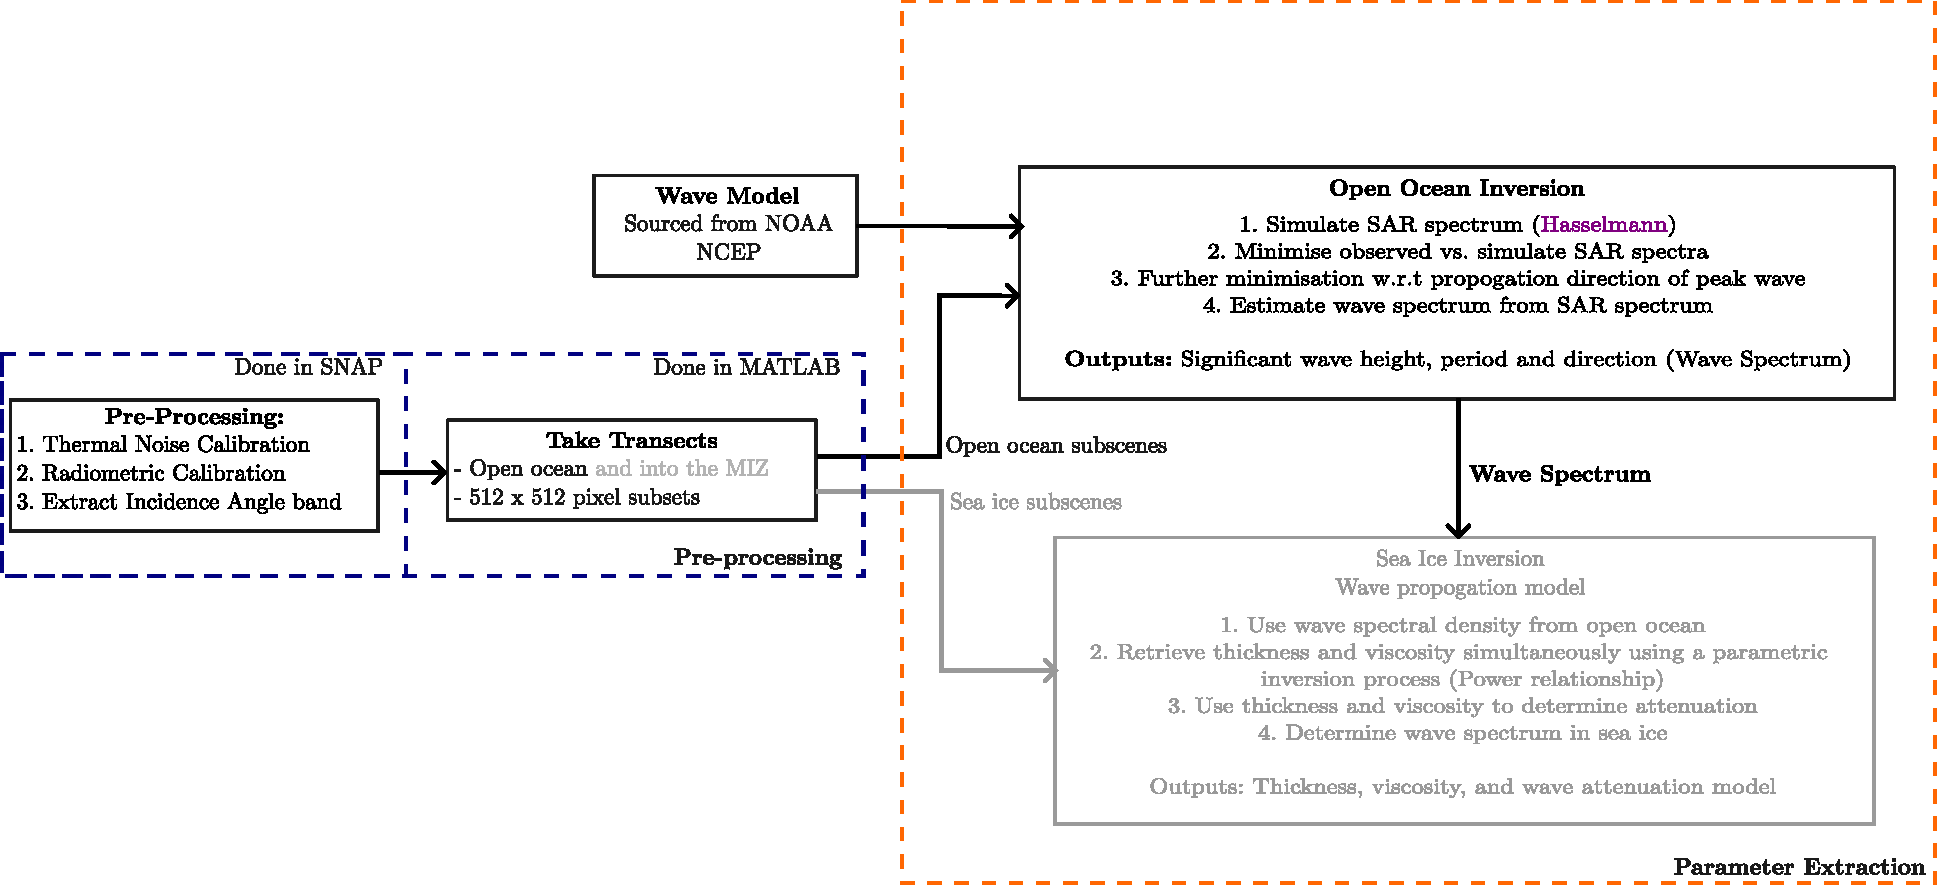
\includegraphics[page=1,width=.9\linewidth]{Figures/PipelineDesign/overall_project.pdf}
%    %\end{tabular}
%  \caption{Test}
%  \label{fig:Test}
% \end{figure}


This chapter begins by providing an overview of the entire pipeline - part of which falls outside of the scope of this project, however, this context is relevant in terms of giving context to the desired results for this project in the context of the broader goals of this pipeline. Each subsequent section will unpack the four main sub-modules within the pipeline in a respective section. Each of these sections will further break down the sub-module into smaller blocks which make up the sub-module. The use of block diagrams allows the process the be understood in terms of the flow of the pipeline, and block diagrams are used throughout this chapter to break down higher-level processes. The variable and function names utilised in this chapter, match those used in the \textsc{Matlab} pipeline.

\section{Overview} \label{sec:systemDesign.overview}

As detailed in xxx, this project required wave parameter extraction for use in a sea ice parameter extraction pipeline. This entire system design is shown as a block diagram in Figure \ref{fig:systemDesign.wholeProject}. It is evident from Figure \ref{fig:systemDesign.wholeProject}, which parts of the \acs{sar} sea ice parameter are relevant to this project. A more detailed block diagram of the wave parameter extraction process is shown in Figure \ref{fig:systemDesign.scope} and within this pipeline, five main functional blocks were identified and are highlighted by five unique colours. [ADD WAVE SPECTRUM GENERATION PIECES]
% Will still change
\begin{figure}[H]
    \centering
    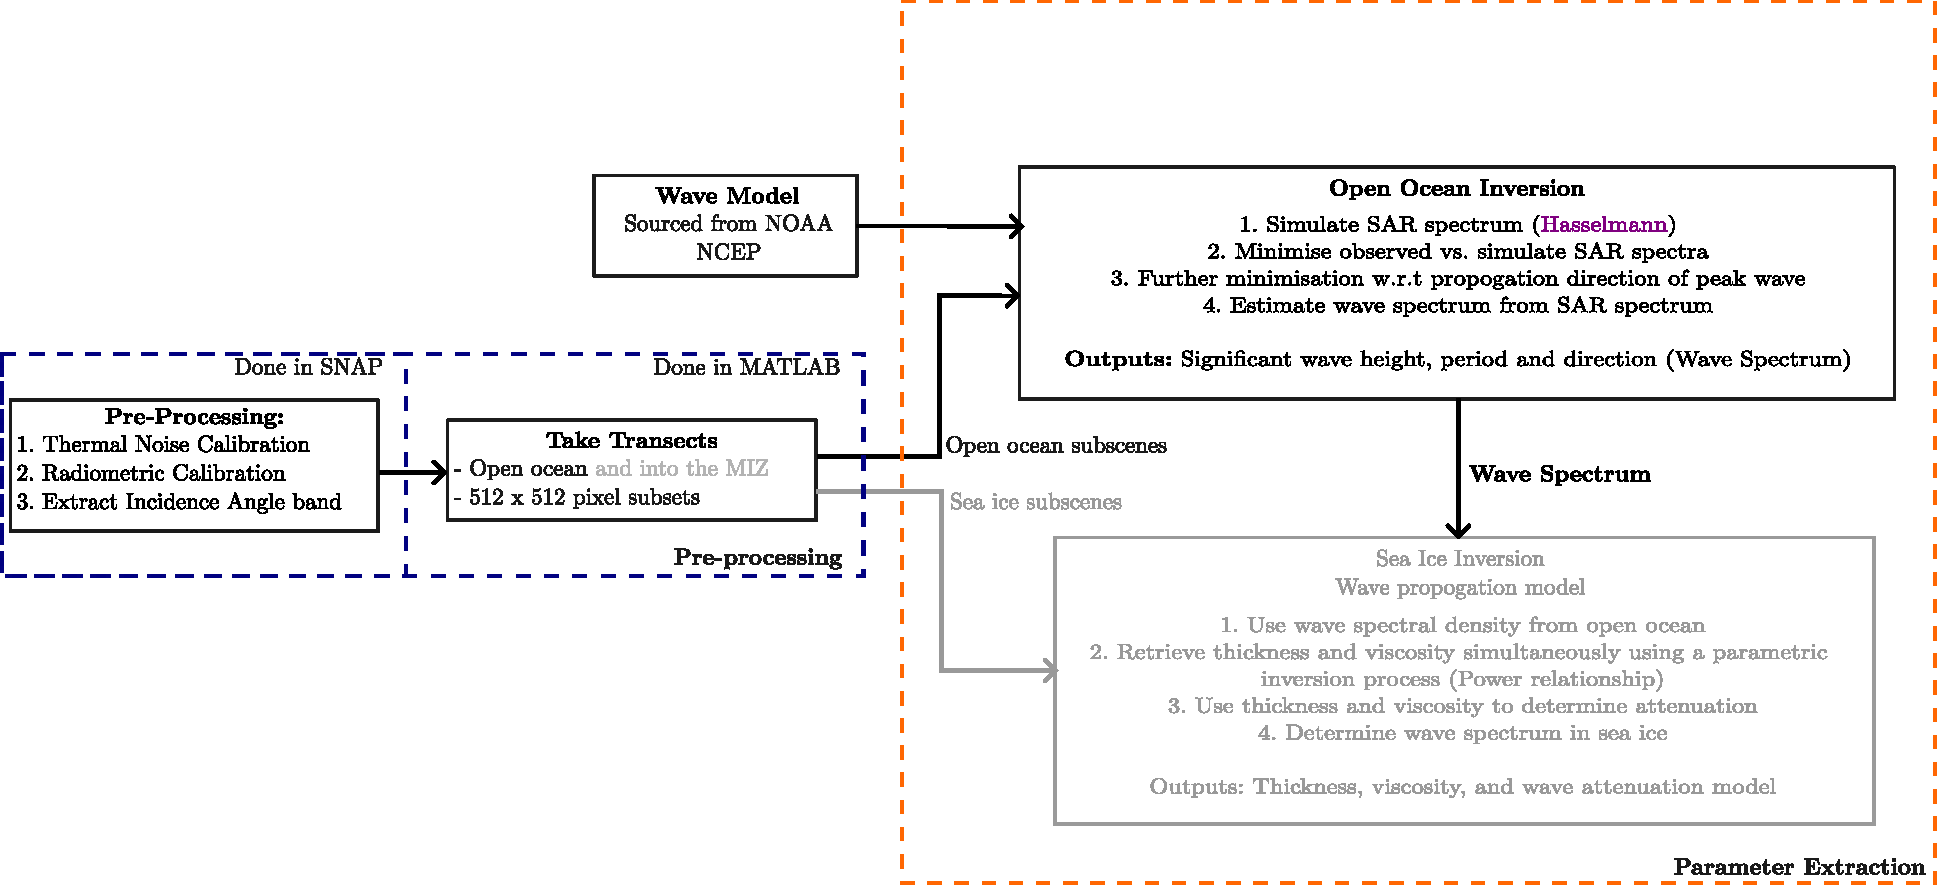
\includegraphics[width=.95\linewidth]{Figures/PipelineDesign/overall_project.pdf}
    \caption{Pipeline system design in the context of the entire parameter extraction process. The scope of this project is shown in black text, with parts of the pipeline outside of the scope, shown in grey.}
    \label{fig:systemDesign.wholeProject}
\end{figure}

% Word better and slim down - ADD DISCUSSION ON WAVE SPECTRUM GENERATION
The five functional blocks were identified as \textsc{pre-processing}, \textsc{metadata extraction}, \textsc{\acs{sar} spectrum calculation}, \textsc{wave spectrum generation}, and \textsc{inversion}. The \textsc{pre-processing} block involves the use of the \ac{snap} Toolbox developed by \ac{esa} as well as \textsc{matlab}, developed by MathWorks Inc. The \textsc{pre-processing} block reads in a downloaded \acs{sar} Level-1 \ac{grd} data file and outputs a \textsc{matlab} structure of \lstinline[columns=fixed]{n} equal-sized transects. These equal-sized transects can be input to the \textsc{inversion} block. The output \ac{netcdf} file from \acs{snap} is used to generate views of \acs{sar} data in \textsc{matlab}, as well as storing the metadata for the \textsc{metadata extraction} block. The \ac{netcdf} file is read by the \textsc{metadata extraction} block and outputs the desired metadata values required for the \textsc{\acs{sar} spectrum calculation} block. The \textsc{\acs{sar} spectrum calculation} block reads in a wave spectrum sourced from \ac{ncep} and generates a \acs{sar} spectrum of the provided wave spectrum. This generated \acs{sar} spectrum is input to the \textsc{inversion} block along with the output of the \textsc{metadata extraction} block. The \textsc{inversion} block outputs the wave parameters from the input \acs{sar} data.
% Will still change
\begin{figure}[H]
    \centering
    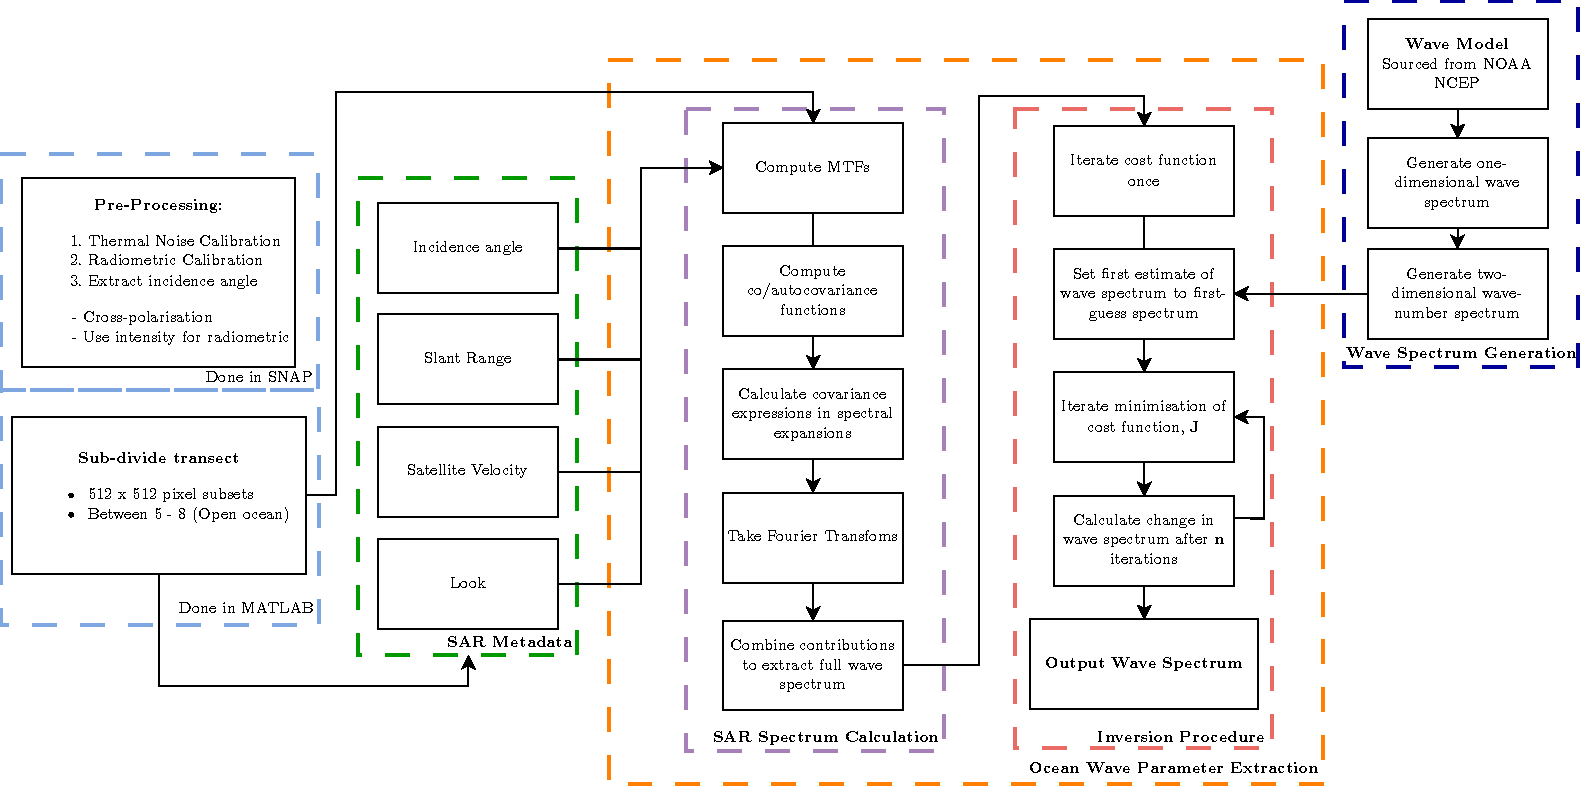
\includegraphics[width=.95\linewidth]{Figures/PipelineDesign/4022_pipeline.pdf}
    \caption{Pipeline system design for this project broken down further than the entire pipeline shown in Figure \ref{fig:systemDesign.wholeProject} containing all the required metadata and external models required, along with the part of the process that they are required.}
    \label{fig:systemDesign.scope}
\end{figure}
%====================================================
% PRE-PROCESSING
%====================================================
\section{Pre-processing} \label{sec:systemDesign.preProcessing}


\subsection{Overview} \label{subsec:systemDesign.preProcessing.Overview}

The pre-processing block of the pipeline was designed in a hybrid manner, with part of the pre-processing done in the \ac{snap} toolbox developed by \ac{esa} prior to the use of \textsc{matlab} tools. The pre-processing block was designed to have an overall function of reading in \ac{s1a} data, apply the desired pre-processing techniques to the \acs{sar} data, and take 512x512 pixel sized transects of this larger \acs{sar} data. The applied pre-processing techniques to calibrate \acs{sar} data for wave parameter extraction were on the recommendation of Giacomo De Carolis and Francesca De Santi of the \acs{irea}, however, discussion around the use of different processing techniques is presented in Chapter \ref{chap:discussion}. The design of this block was designed to keep pre-processing outside of the \textsc{matlab} environment to a minimum, through the use of external tools. 

The pre-processing block had six notable stages: Thermal noise calibration of \acs{s1a} \acs{grd} data, radiometric calibration of these data, extraction of individual pixel incidence angle, exporting calibrated \acs{grd} data to a usable format for \textsc{matlab}, reading in the exported data, and taking 512x512 pixel transects of the larger \acs{sar} data. The flow of this block of the pipeline is shown graphically in Figure \ref{fig:systemDesign.preProcessing.blockDiagram}.

\begin{figure}[H]
    \centering
    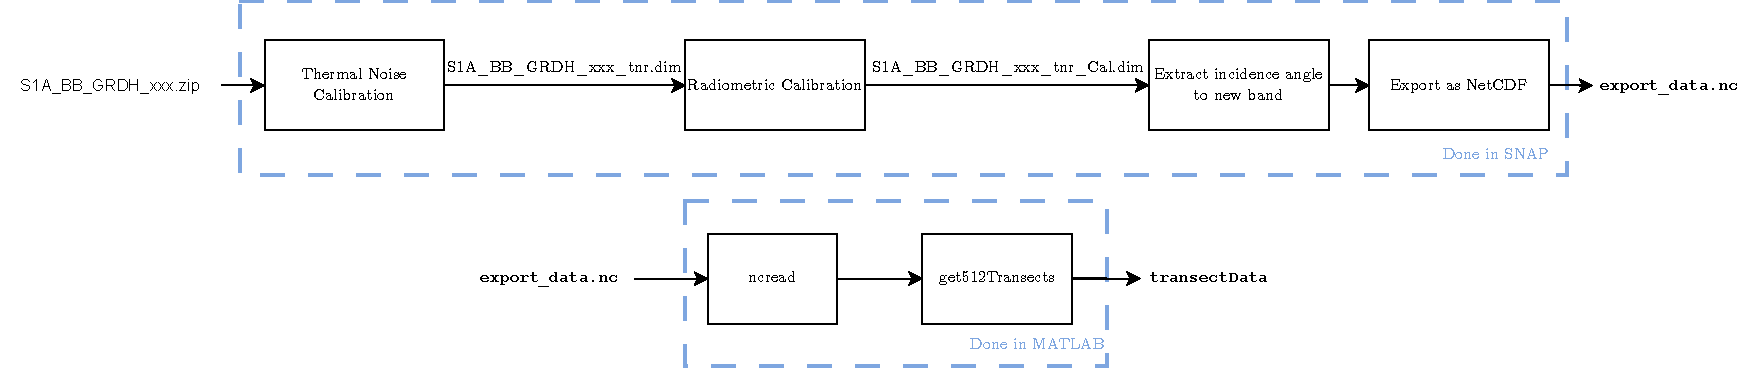
\includegraphics[width=.95\linewidth]{Figures/PipelineDesign/pre_processing.pdf}
    \caption{Block diagram depicting an expanded pre-processing sub-block of Figure \ref{fig:systemDesign.scope}}
    \label{fig:systemDesign.preProcessing.blockDiagram}
\end{figure}

\subsection{Thermal Noise Calibration} \label{subsec:systemDesign.preProcessing.thermalNoise}

After obtaining \acs{grd} \acs{sar} data from \href{scihub.copernicus.eu/dhus/#/home}{Copernicus SciHub}, the first sub-block of the pre-processing block was Thermal Noise Calibration

\subsection{Radiometric Calibration} \label{subsec:systemDesign.preProcessing.radiometric}

\subsection{Incidence Angle Extraction} \label{subsec:systemDesign.preProcessing.incidenceAngle}

\subsection{\acs{netcdf} Export} \label{subsec:systemDesign.preProcessing.exportNetCDF}
% Discuss why netcdf
\subsection{MATLAB Data Import} \label{subsec:systemDesign.preProcessing.importData}

The first sub-block in the \textsc{matlab} implementation of the pre-processing block was called \lstinline{ncread}. As discussed above, the \acs{netcdf} file format was used for all imported data into \textsc{matlab} due to its use in xxxx.

\subsection{Take Transects and Subdivide Data} \label{subsec:systemDesign.preProcessing.transects}

The most important part of the pre-processing for wave parameter extraction for use in sea ice parameter extraction is the ability to 'follow' the flow of ocean waves into the \acs{miz}. To achieve this, transects of a fixed size are taken of open ocean scenes as well as sea ice scenes. This allows the way in which ocean waves propagate through sea ice to be studied, and due to this, sea ice parameters are able to be extracted using the models described in Section \ref{subsec:litReview.sarCharac.seaIceWaveModelling}. As per \cite{Wadhams2004,DeSanti2018} the size of these transects should be 512x512 pixels in size. Taking transects of a larger image in \textsc{matlab} is relatively straightforward, however, these transects need to be able to be taken at an angle to follow the direction of the visible ocean waves. If the ocean wave direction is not followed, this could cause issues in determining the way in which ocean waves are attenuated in the \acs{miz}. Along with this, the transect needs to start at a certain location of the whole scene. Due to the fact that latitude and longitude are not encoded in the \acs{s1a} \ac{grd} data, it was decided that a pixel starting position would be used to determine the starting position.

Due to the way in which \textsc{matlab} indexes arrays, which is counter-intuitive to other programming languages, with the initial index being given a value of \textsc{1}, a check that the start location of the first transect was a valid index in the imported sarData needed to be conducted. This was achieved using a simple \lstinline{if} statement.

\begin{figure}[H]
    \centering
    \includegraphics[width=.95\linewidth]{Figures/PipelineDesign/transects_w_SAR.pdf}
    \caption{Transect of full \acs{sar} data geometry.}
    \label{fig:systemDesign.transects}
\end{figure}



Obtain SAR look over region of interest - want VV and HH polarisation data (mainly used VV)

Start by doing pre-processing in SNAP ESA tool
\begin{enumerate}
    \item Thermal noise calibration
    \item Radiometric Calibration using intensity in linear units
\end{enumerate}

Export pre-processed data as netCDF file and save path

Import path into MATLAB. Will save desired band data as n x m double of intensity/amplitude values. Able to plot full look in MATLAB. [Need to figure out how to get image rotated by 180 deg ccw/cw]

Transects:
use get512Transects function. Enter data to take transect of, top left x coord, top left y coord, angle of the transects from + x axis, number of transects(n). Outputs a n x 2 matrix of sar data, and corner pixel values.

Can plot full look showing the location of transects in full look using defined colours and number of transects. Can plot individual transects. Transects will be used to see the evolution of wave parameters across a region

Metadata:

All the required metadata can be extracted using the extractMetadata function. Need to provide the ncread(path,'metadata') output. This returns a structure with the metadata name and value. Certain, different values can be extracted using the filterAttributes function

%====================================================
% WAVE SPECTRUM GENERATION
%====================================================
\section{Wave Spectrum Generation} \label{sec:systemDesign.waveSpectrum}



\subsection{Overview} \label{subsec:systemDesign.waveSpectrum.Overview}

\begin{figure}[H]
    \centering
    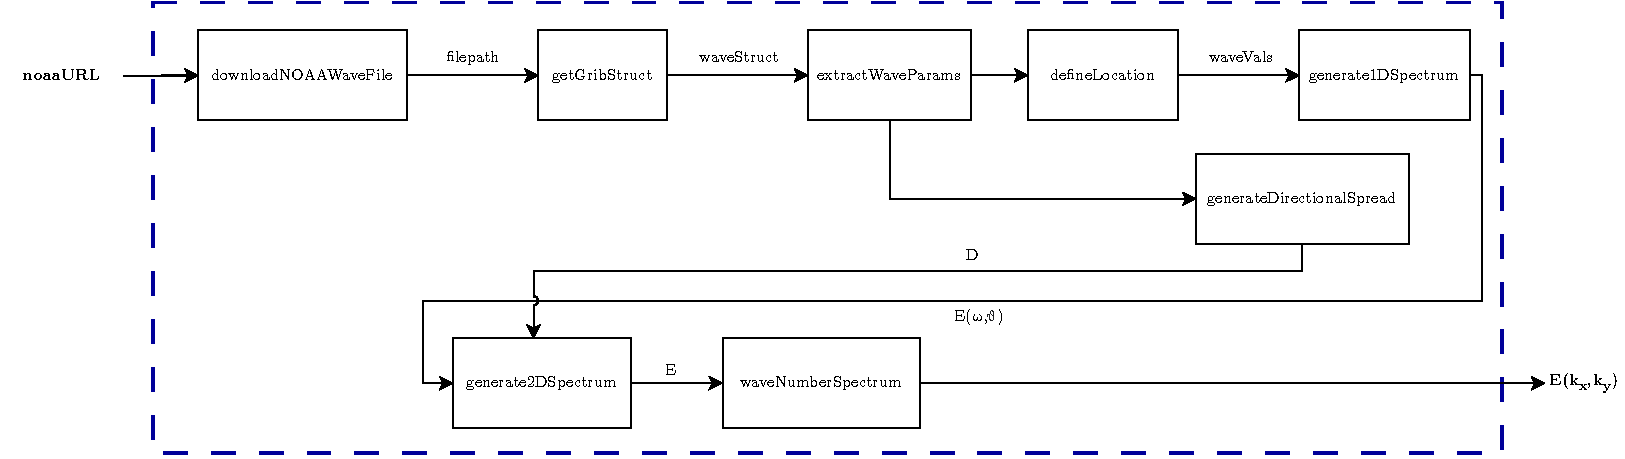
\includegraphics[width=.95\linewidth]{Figures/PipelineDesign/wave_spectrum.pdf}
    \caption{Block diagram depicting an expanded wave spectrum generation sub-block of Figure \ref{fig:systemDesign.scope}}
    \label{fig:systemDesign.wavesSpectrum.blockDiagram}
\end{figure}

\subsection{Wave Data Download} \label{subsec:systemDesign.waveSpectrum.download}

\subsection{GRIB2 to \acs{netcdf} Conversion} \label{subsec:systemDesign.waveSpectrum.toNetCDF}

\subsection{Wave Parameter Extraction} \label{subsec:systemDesign.waveSpectrum.parameters}


When examining the latitude and longitude values obtained from \acs{ncep}, it was noted that these data points contained decimal points of order $10^{-6}$. This proved an issue when trying to index the original downloaded wave data to access a subset of these data using the code snippet depicted in Listing \ref{code:latLonExtract.initial}. This code resulted in none of the desired data being found.

\begin{lstlisting}[caption={Initial implementation of \textsc{Matlab} code to extract wave parameters at certain geographical location.},label={code:latLonExtract.initial}]
lonVal = 45.25;
lonIndex = find(lon == lonVal);
\end{lstlisting}

In order to mitigate this, an investigation into the resolution of decimal degrees was conducted in order to match the spatial resolution of wave data to the corresponding \acs{sar} resolution. It was found that 5 decimal places allowed a worst-case resolution of 1.11\,m \cite{decimalDegreesWikipedia}. In the case of \acs{s1a}, such resolution is adequate, due to the satellite's highest spatial resolution of 9x9\,m resolution for \acs{grd} data \cite{sentinel1ProductDef}. Using this information, it was decided to update the code in Listing \ref{code:latLonExtract.initial} to the code seen in Listing \ref{code:latLonExtract.round} to allow accurate indexing of spatial coordinates without loss of spatial resolution.

\begin{lstlisting}[caption={Updated implementation of \textsc{Matlab} code to extract wave parameters at certain geographical location.},label={code:latLonExtract.round}]
lonVal = 45.25;
lonIndex = find(round(lon,5) == lonVal);
\end{lstlisting}


%\subsection{Location Definition} \label{subsec:systemDesign.waveSpectrum.defineLoc}
% Put in 1D wave spectrum Generation

\subsection{One Dimensional Wave Spectrum} \label{subsec:systemDesign.waveSpectrum.1DSpectrum}

Whilst the generation of a one-dimensional wave spectrum is only represented by one sub-block in Figure \ref{fig:systemDesign.wavesSpectrum.blockDiagram}, the generation of this spectrum is vital to forming the foundation of the two-dimensional wave spectrum which is used as a first-guess wave spectrum when minimising the cost function described in Equation \ref{eq:hh.inversion.J}. As discussed in Section \ref{subsec:theory.waves.modelling}, the most widely used wave model is the \acs{jonswap} model, and implementing this spectrum required a careful approach in order to ensure accurate modelling of waves was done using the downloaded wave data detailed in Section \ref{subsec:systemDesign.waveSpectrum.download}.

In order to construct a \acs{jonswap} wave model, $E(\omega)$, the equations detailed in Section \ref{subsec:theory.waves.modelling} were implemented in \textsc{matlab} as outlined in the pseudocode given in Algorithm \ref{alg:jonswap} where $H_{1/3}$ and $w_{peak}$ are wave parameters as detailed in Section \ref{subsec:theory.waves.waveSpectrum} and $\omega$ is the range of frequencies over which to generate the wave spectrum for. as well as defining which geographical coordinate to construct the wave spectrum for. 
%% Mention how we know what gamma value to use


\begin{figure}[H]
  \vspace{0.5cm}
  \centering
  \captionsetup{type=figure}
  \begin{minipage}{.75\linewidth}
    \begin{algorithm}[H]
      \caption{\acs{jonswap} wave spectrum generation\label{alg:jonswap}}

      \DontPrintSemicolon
      \SetAlgoLined
      \SetKwInOut{Input}{input}\SetKwInOut{Output}{output}\SetKwInOut{Parameter}{parameter}

      \Input{Wave parameters, $H_{1/3}$, $\omega_{peak}$ \\ Frequency range, $\omega$}
      \Output{\acs{jonswap} wave spectrum, $E(\omega)$}
      \Parameter{Peak enhancement factor, $\gamma$} % What is parameter

      \BlankLine
          \Begin{
          $g \leftarrow 9.81$\;
          $\alpha \leftarrow 0.2 \cdot H_{1/3}^{2} \cdot \frac{\omega_{peak}^{4}}{g^{2}}$ \;
          \If{$\gamma < 1$ or $\gamma > 7$}{
            % \If{$\gamma \neq 0$}{
            %     %\textbf{Display} warning message: "Warning: gamma value in wave_spectrum function outside validity range, using DNV formula"\;
            % }
            $k \leftarrow \frac{2\pi}{\omega_{0} \cdot \sqrt{H_{s}}}$\;
           \If{$k \leq 3.6$}{
                $\gamma \leftarrow 5$\;
           }
           \eIf{$k \leq 5$}{
                $\gamma \leftarrow \exp(5.75 - 1.15 \cdot k)$\;
           }{
                $\gamma \leftarrow 1$\;
           }
          }
        \For{$k$ in $1$ to $\text{length}(\omega)$}{
        \If{$\omega(k) < \omega_{peak}$}{
        $\sigma \leftarrow 0.07$\;
    }
    \Else{
        $\sigma \leftarrow 0.09$\;
    }
    
    $E1 \leftarrow \alpha \cdot g^2 \cdot (\omega(k)^{-5}) \cdot \exp\left(-\frac{5}{4} \cdot \left ( \frac{\omega_{peak}}{\omega(k)}\right)^4\right)$\;
    $exponent \leftarrow  \exp\left(- \frac{(\omega(k) - \omega_0)^2}{2 \cdot (\sigma \cdot \omega_0)^2}\right) $ \;
    $E2 \leftarrow \gamma^{exponent}$\;
    
    $E \leftarrow E1 \cdot E2$\;
}
        }
      \vspace{0.5cm}
    \end{algorithm}
  \end{minipage}
\end{figure}


Extending Algorithm \ref{alg:jonswap} to allow multiple spectra to be calculated at multiple latitudes and longitudes allowed the validity of the spectrum generation to be validated as plotting multiple wave spectra on the same set of axes allowed the way in which the wave spectra change as they approach the shore to be determined. This analysis is discussed in Section xxx and example plots obtained using the \href{https://github.com/JNSRYA006/sar-parameter-extraction-pipeline/blob/main/functions/waveSpectra/generateSingleJONSWAP.m}{\lstinline{generateSingleJONSWAP}} and \href{https://github.com/JNSRYA006/sar-parameter-extraction-pipeline/blob/main/functions/waveSpectra/generateMultipleJONSWAP.m}{\lstinline{generateMultipleJONSWAP}} functions are shown in Figure \ref{fig:systemDesign.1DSampleWaveSpectrum}. 

% \begin{figure}[H]
% \centering
% \begin{subfigure}{0.48\linewidth} % Use \begin{subfigure} instead of \begin{subfigure}
%     \resizebox{\linewidth}{!}{% This file was created by matlab2tikz.
%
%The latest updates can be retrieved from
%  http://www.mathworks.com/matlabcentral/fileexchange/22022-matlab2tikz-matlab2tikz
%where you can also make suggestions and rate matlab2tikz.
%
\definecolor{mycolor1}{rgb}{0.00000,0.44700,0.74100}%
%
\begin{tikzpicture}

\begin{axis}[%
width=4.476in,
height=3.524in,
at={(0.803in,0.523in)},
scale only axis,
unbounded coords=jump,
xmin=0,
xmax=7,
xtick={0,1.5707963267949,3.14159265358979,4.71238898038469,6.28318530717959},
xticklabels={{0},{$\pi\text{/2}$},{$\pi$},{$\text{3}\pi\text{/2}$},{$\text{2}\pi$}},
xlabel style={font=\color{white!15!black}},
xlabel={$\omega\text{ [rad/s]}$},
ymin=0,
ymax=0.04,
ylabel style={font=\color{white!15!black}},
ylabel={$\text{E(}\omega\text{) [m}^\text{2}\text{/rad/Hz]}$},
axis background/.style={fill=white},
title style={font=\bfseries},
%title={$\text{One-dimensional wave spectrum, E(}\omega\text{) at -34S, 17.25E}$},
xmajorgrids,
ymajorgrids,
legend style={legend cell align=left, align=left, draw=white!15!black}
]
\addplot [color=mycolor1]
  table[row sep=crcr]{%
0	nan\\
0.0122958616578857	0\\
0.0245917233157714	0\\
0.0368875849736571	0\\
0.0491834466315427	0\\
0.0614793082894284	0\\
0.0737751699473141	0\\
0.0860710316051998	0\\
0.0983668932630855	0\\
0.110662754920971	0\\
0.122958616578857	0\\
0.135254478236743	0\\
0.147550339894628	0\\
0.159846201552514	0\\
0.1721420632104	0\\
0.184437924868285	0\\
0.196733786526171	0\\
0.209029648184057	0\\
0.221325509841942	0\\
0.233621371499828	0\\
0.245917233157714	0\\
0.258213094815599	0\\
0.270508956473485	0\\
0.282804818131371	0\\
0.295100679789256	5.41302879763333e-307\\
0.307396541447142	1.4351658983951e-260\\
0.319692403105028	1.39801651640755e-222\\
0.331988264762914	2.95955173493782e-191\\
0.344284126420799	3.06617261869068e-165\\
0.356579988078685	1.71585454184354e-143\\
0.368875849736571	3.36115162791715e-125\\
0.381171711394456	9.99471845091621e-110\\
0.393467573052342	1.44074967318733e-96\\
0.405763434710228	2.54134308132756e-85\\
0.418059296368113	1.15384979645612e-75\\
0.430355158025999	2.46010694641464e-67\\
0.442651019683885	4.01707121559874e-60\\
0.45494688134177	7.49671131280128e-54\\
0.467242742999656	2.22288404307939e-48\\
0.479538604657542	1.3753760835859e-43\\
0.491834466315427	2.22745866619101e-39\\
0.504130327973313	1.14105811314078e-35\\
0.516426189631199	2.16730148431401e-32\\
0.528722051289085	1.74501685936915e-29\\
0.54101791294697	6.67054290550385e-27\\
0.553313774604856	1.33294088654399e-24\\
0.565609636262742	1.51145852287043e-22\\
0.577905497920627	1.0433270916913e-20\\
0.590201359578513	4.65664898554377e-19\\
0.602497221236399	1.41551545559892e-17\\
0.614793082894284	3.06504085545376e-16\\
0.62708894455217	4.91508596715723e-15\\
0.639384806210056	6.03782647089776e-14\\
0.651680667867941	5.85166582657271e-13\\
0.663976529525827	4.59100381164424e-12\\
0.676272391183713	2.98235025750544e-11\\
0.688568252841599	1.63618607596188e-10\\
0.700864114499484	7.71435740175365e-10\\
0.71315997615737	3.17422780050511e-09\\
0.725455837815256	1.15545266932238e-08\\
0.737751699473141	3.76593918002615e-08\\
0.750047561131027	1.11082567474578e-07\\
0.762343422788913	2.99365257438456e-07\\
0.774639284446798	7.43398794457705e-07\\
0.786935146104684	1.71393732492197e-06\\
0.79923100776257	3.6936978163335e-06\\
0.811526869420455	7.48610717182671e-06\\
0.823822731078341	1.43464290828625e-05\\
0.836118592736227	2.61246562604755e-05\\
0.848414454394112	4.54036148623333e-05\\
0.860710316051998	7.56117606150625e-05\\
0.873006177709884	0.000121089372916668\\
0.88530203936777	0.000187089786772187\\
0.897597901025655	0.000279703606526386\\
0.909893762683541	0.000405702450085907\\
0.922189624341426	0.000572308176547121\\
0.934485485999312	0.000786902195884214\\
0.946781347657198	0.00105669606424971\\
0.959077209315084	0.00138838834019309\\
0.971373070972969	0.00178783338397504\\
0.983668932630855	0.00225974569705202\\
0.995964794288741	0.00280745915996462\\
1.00826065594663	0.00343275496464683\\
1.02055651760451	0.00413576600873186\\
1.0328523792624	0.00491495977802167\\
1.04514824092028	0.00576719685342651\\
1.05744410257817	0.00668785847600663\\
1.06973996423605	0.00767103419145496\\
1.08203582589394	0.00870975936699404\\
1.09433168755183	0.0097962920536587\\
1.10662754920971	0.0109224188636112\\
1.1189234108676	0.0120797798007726\\
1.13121927252548	0.0132602018978306\\
1.14351513418337	0.0144560307440969\\
1.15581099584125	0.0156604473784329\\
1.16810685749914	0.0168677556407375\\
1.18040271915703	0.0180736222488931\\
1.19269858081491	0.0192752491472963\\
1.2049944424728	0.0204714557558278\\
1.21729030413068	0.0216626483564445\\
1.22958616578857	0.0228506556097147\\
1.24188202744645	0.0240384135360737\\
1.25417788910434	0.0252294904939306\\
1.26647375076223	0.0264274529344006\\
1.27876961242011	0.0276350862726403\\
1.291065474078	0.0288535024756524\\
1.30336133573588	0.0300811872588852\\
1.31565719739377	0.0313130648442189\\
1.32795305905165	0.0325396852882558\\
1.34024892070954	0.0337466641153829\\
1.35254478236743	0.0349145188355605\\
1.36484064402531	0.0360190415875961\\
1.3771365056832	0.0370323108877261\\
1.38943236734108	0.0379243714742074\\
1.40172822899897	0.0386655021114703\\
1.41402409065685	0.0392288631897149\\
1.42631995231474	0.0395931988386078\\
1.43861581397263	0.0397451987880671\\
1.45091167563051	0.0397009837064543\\
1.4632075372884	0.0395060933162202\\
1.47550339894628	0.0391703952648501\\
1.48779926060417	0.0387059506556059\\
1.50009512226205	0.0381276193041899\\
1.51239098391994	0.0374522472133023\\
1.52468684557783	0.0366977905296433\\
1.53698270723571	0.0358824534634019\\
1.5492785688936	0.0350239067515314\\
1.56157443055148	0.0341386357865274\\
1.57387029220937	0.033241447182027\\
1.58616615386725	0.0323451427488864\\
1.59846201552514	0.0314603532066003\\
1.61075787718303	0.0305955119179262\\
1.62305373884091	0.0297569418708591\\
1.6353496004988	0.0289490265523619\\
1.64764546215668	0.0281744362672717\\
1.65994132381457	0.0274343846835443\\
1.67223718547245	0.0267288948374096\\
1.68453304713034	0.0260570586376697\\
1.69682890878822	0.0254172784703886\\
1.70912477044611	0.0248074834845985\\
1.721420632104	0.024225316400738\\
1.73371649376188	0.023668289227364\\
1.74601235541977	0.0231339081746281\\
1.75830821707765	0.0226197694201764\\
1.77060407873554	0.0221236283185714\\
1.78289994039342	0.0216434452374737\\
1.79519580205131	0.0211774115218765\\
1.8074916637092	0.0207239591846428\\
1.81978752536708	0.0202817578397189\\
1.83208338702497	0.0198497021705522\\
1.84437924868285	0.0194268928954684\\
1.85667511034074	0.0190126137886203\\
1.86897097199862	0.0186063068732881\\
1.88126683365651	0.0182075474549375\\
1.8935626953144	0.0178160202313337\\
1.90585855697228	0.0174314973270267\\
1.91815441863017	0.0170538187637728\\
1.93045028028805	0.0166828756042898\\
1.94274614194594	0.0163185957954444\\
1.95504200360382	0.0159609325850235\\
1.96733786526171	0.0156098552867384\\
1.9796337269196	0.015265342112225\\
1.99192958857748	0.0149273747670556\\
2.00422545023537	0.0145959345109985\\
2.01652131189325	0.0142709994027779\\
2.02881717355114	0.0139525424796016\\
2.04111303520902	0.0136405306563983\\
2.05340889686691	0.0133349241651845\\
2.0657047585248	0.0130356763886258\\
2.07800062018268	0.0127427339721329\\
2.09029648184057	0.0124560371249502\\
2.10259234349845	0.0121755200424896\\
2.11488820515634	0.0119011113998192\\
2.12718406681422	0.0116327348801607\\
2.13947992847211	0.011370309712995\\
2.15177579012999	0.0111137512044894\\
2.16407165178788	0.0108629712489418\\
2.17636751344577	0.0106178788142673\\
2.18866337510365	0.0103783803976124\\
2.20095923676154	0.0101443804493013\\
2.21325509841942	0.00991578176473845\\
2.22555096007731	0.00969248584482827\\
2.2378468217352	0.00947439322604724\\
2.25014268339308	0.00926140378164897\\
2.26243854505097	0.0090534169956585\\
2.27473440670885	0.00885033221138453\\
2.28703026836674	0.00865204885617913\\
2.29932613002462	0.00845846664413426\\
2.31162199168251	0.00826948575833719\\
2.3239178533404	0.00808500701422663\\
2.33621371499828	0.00790493200550391\\
2.34850957665617	0.00772916323396475\\
2.36080543831405	0.00755760422452847\\
2.37310129997194	0.00739015962665654\\
2.38539716162982	0.00722673530327022\\
2.39769302328771	0.00706723840819925\\
2.40998888494559	0.00691157745312068\\
2.42228474660348	0.0067596623648772\\
2.43458060826137	0.00661140453400037\\
2.44687646991925	0.00646671685520286\\
2.45917233157714	0.00632551376054758\\
2.47146819323502	0.00618771124594853\\
2.48376405489291	0.00605322689160874\\
2.49605991655079	0.00592197987695489\\
2.50835577820868	0.00579389099058502\\
2.52065163986657	0.00566888263570622\\
2.53294750152445	0.00554687883150177\\
2.54524336318234	0.00542780521083287\\
2.55753922484022	0.00531158901464808\\
2.56983508649811	0.00519815908344373\\
2.58213094815599	0.00508744584609102\\
2.59442680981388	0.00497938130631981\\
2.60672267147177	0.00487389902712567\\
2.61901853312965	0.00477093411334424\\
2.63131439478754	0.00467042319261705\\
2.64361025644542	0.00457230439495386\\
2.65590611810331	0.00447651733107909\\
2.66820197976119	0.00438300306973388\\
2.68049784141908	0.00429170411409041\\
2.69279370307697	0.00420256437742111\\
2.70508956473485	0.00411552915815301\\
2.71738542639274	0.00403054511442532\\
2.72968128805062	0.00394756023825787\\
2.74197714970851	0.00386652382942774\\
2.75427301136639	0.00378738646914243\\
2.76656887302428	0.00371009999358922\\
2.77886473468217	0.00363461746743274\\
2.79116059634005	0.00356089315732546\\
2.80345645799794	0.00348888250548924\\
2.81575231965582	0.00341854210342006\\
2.82804818131371	0.00334982966576232\\
2.84034404297159	0.00328270400439414\\
2.85263990462948	0.00321712500276036\\
2.86493576628737	0.00315305359048552\\
2.87723162794525	0.00309045171829528\\
2.88952748960314	0.00302928233327117\\
2.90182335126102	0.0029695093544601\\
2.91411921291891	0.00291109764885714\\
2.92641507457679	0.00285401300777748\\
2.93871093623468	0.00279822212363068\\
2.95100679789256	0.00274369256710825\\
2.96330265955045	0.00269039276479353\\
2.97559852120834	0.00263829197720089\\
2.98789438286622	0.00258736027724954\\
3.00019024452411	0.00253756852917576\\
3.01248610618199	0.00248888836788607\\
3.02478196783988	0.00244129217875227\\
3.03707782949776	0.00239475307784859\\
3.04937369115565	0.00234924489262979\\
3.06166955281354	0.0023047421430484\\
3.07396541447142	0.0022612200231083\\
3.08626127612931	0.00221865438285134\\
3.09855713778719	0.00217702171077273\\
3.11085299944508	0.00213629911666074\\
3.12314886110296	0.00209646431485547\\
3.13544472276085	0.00205749560792113\\
3.14774058441874	0.00201937187072593\\
3.16003644607662	0.00198207253492326\\
3.17233230773451	0.00194557757382764\\
3.18462816939239	0.00190986748767868\\
3.19692403105028	0.00187492328928602\\
3.20921989270816	0.00184072649004824\\
3.22151575436605	0.00180725908633834\\
3.23381161602394	0.00177450354624858\\
3.24610747768182	0.00174244279668723\\
3.25840333933971	0.00171106021081969\\
3.27069920099759	0.0016803395958467\\
3.28299506265548	0.00165026518111192\\
3.29529092431336	0.00162082160653164\\
3.30758678597125	0.00159199391133908\\
3.31988264762914	0.00156376752313587\\
3.33217850928702	0.00153612824724346\\
3.34447437094491	0.00150906225634721\\
3.35677023260279	0.00148255608042589\\
3.36906609426068	0.00145659659695957\\
3.38136195591856	0.00143117102140895\\
3.39365781757645	0.00140626689795909\\
3.40595367923434	0.00138187209052092\\
3.41824954089222	0.00135797477398379\\
3.43054540255011	0.00133456342571239\\
3.44284126420799	0.00131162681728186\\
3.45513712586588	0.00128915400644448\\
3.46743298752376	0.00126713432932197\\
3.47972884918165	0.00124555739281723\\
3.49202471083954	0.00122441306723957\\
3.50432057249742	0.00120369147913769\\
3.51661643415531	0.00118338300433464\\
3.52891229581319	0.00116347826115928\\
3.54120815747108	0.00114396810386871\\
3.55350401912896	0.00112484361625655\\
3.56579988078685	0.0011060961054416\\
3.57809574244473	0.00108771709583218\\
3.59039160410262	0.00106969832326091\\
3.60268746576051	0.00105203172928534\\
3.61498332741839	0.00103470945564963\\
3.62727918907628	0.0010177238389028\\
3.63957505073416	0.00100106740516895\\
3.65187091239205	0.000984732865065375\\
3.66416677404994	0.000968713108764074\\
3.67646263570782	0.00095300120119279\\
3.68875849736571	0.00093759037737141\\
3.70105435902359	0.000922474037879949\\
3.71335022068148	0.000907645744454282\\
3.72564608233936	0.000893099215705966\\
3.73794194399725	0.000878828322962575\\
3.75023780565513	0.000864827086225059\\
3.76253366731302	0.000851089670238769\\
3.77482952897091	0.000837610380674829\\
3.78712539062879	0.000824383660418703\\
3.79942125228668	0.000811404085962812\\
3.81171711394456	0.00079866636390022\\
3.82401297560245	0.000786165327516438\\
3.83630883726033	0.000773895933476511\\
3.84860469891822	0.000761853258604621\\
3.86090056057611	0.000750032496753526\\
3.87319642223399	0.000738428955761214\\
3.88549228389188	0.000727038054492271\\
3.89778814554976	0.000715855319961465\\
3.91008400720765	0.000704876384537197\\
3.92237986886553	0.000694096983222478\\
3.93467573052342	0.000683512951011199\\
3.94697159218131	0.000673120220317491\\
3.95926745383919	0.000662914818476088\\
3.97156331549708	0.000652892865311599\\
3.98385917715496	0.000643050570774724\\
3.99615503881285	0.000633384232643455\\
4.00845090047073	0.000623890234287399\\
4.02074676212862	0.000614565042493382\\
4.03304262378651	0.000605405205350579\\
4.04533848544439	0.000596407350193436\\
4.05763434710228	0.000587568181600735\\
4.06993020876016	0.000578884479449159\\
4.08222607041805	0.00057035309701982\\
4.09452193207593	0.000561970959156189\\
4.10681779373382	0.000553735060471986\\
4.1191136553917	0.000545642463607562\\
4.13140951704959	0.000537690297533413\\
4.14370537870748	0.00052987575589945\\
4.15600124036536	0.000522196095428724\\
4.16829710202325	0.000514648634354346\\
4.18059296368113	0.00050723075089834\\
4.19288882533902	0.00049993988179127\\
4.2051846869969	0.000492773520831441\\
4.21748054865479	0.00048572921748257\\
4.22977641031268	0.000478804575508837\\
4.24207227197056	0.000471997251646233\\
4.25436813362845	0.000465304954309197\\
4.26666399528633	0.000458725442331523\\
4.27895985694422	0.000452256523740597\\
4.29125571860211	0.000445896054563984\\
4.30355158025999	0.000439641937667487\\
4.31584744191788	0.000433492121623766\\
4.32814330357576	0.000427444599610678\\
4.34043916523365	0.000421497408338488\\
4.35273502689153	0.000415648627005148\\
4.36503088854942	0.000409896376278856\\
4.37732675020731	0.000404238817307136\\
4.38962261186519	0.000398674150751693\\
4.40191847352308	0.000393200615848326\\
4.41421433518096	0.000387816489491206\\
4.42651019683885	0.000382520085340833\\
4.43880605849673	0.000377309752955029\\
4.45110192015462	0.000372183876942308\\
4.46339778181251	0.000367140876137024\\
4.47569364347039	0.000362179202795692\\
4.48798950512828	0.000357297341813879\\
4.50028536678616	0.000352493809963128\\
4.51258122844405	0.000347767155147345\\
4.52487709010193	0.000343115955678117\\
4.53717295175982	0.000338538819568452\\
4.5494688134177	0.000334034383844427\\
4.56176467507559	0.000329601313874257\\
4.57406053673348	0.000325238302714321\\
4.58635639839136	0.000320944070471665\\
4.59865226004925	0.000316717363682552\\
4.61094812170713	0.000312556954706612\\
4.62324398336502	0.00030846164113618\\
4.6355398450229	0.000304430245220401\\
4.64783570668079	0.000300461613303707\\
4.66013156833868	0.000296554615278295\\
4.67242742999656	0.000292708144050196\\
4.68472329165445	0.000288921115018604\\
4.69701915331233	0.000285192465568094\\
4.70931501497022	0.000281521154573383\\
4.7216108766281	0.000277906161916305\\
4.73390673828599	0.000274346488014674\\
4.74620259994388	0.000270841153362717\\
4.75849846160176	0.000267389198082769\\
4.77079432325965	0.000263989681487935\\
4.78309018491753	0.000260641681655428\\
4.79538604657542	0.000257344295010299\\
4.8076819082333	0.000254096635919287\\
4.81997776989119	0.000250897836294526\\
4.83227363154908	0.000247747045206839\\
4.84456949320696	0.000244643428508389\\
4.85686535486485	0.000241586168464416\\
4.86916121652273	0.000238574463393844\\
4.88145707818062	0.000235607527318515\\
4.8937529398385	0.000232684589620834\\
4.90604880149639	0.000229804894709597\\
4.91834466315427	0.000226967701693801\\
4.93064052481216	0.000224172284064218\\
4.94293638647005	0.000221417929382543\\
4.95523224812793	0.000218703938977918\\
4.96752810978582	0.000216029627650631\\
4.9798239714437	0.000213394323382829\\
4.99211983310159	0.000210797367056043\\
5.00441569475948	0.000208238112175362\\
5.01671155641736	0.000205715924600084\\
5.02900741807525	0.000203230182280682\\
5.04130327973313	0.000200780275001916\\
5.05359914139102	0.000198365604131947\\
5.0658950030489	0.000195985582377289\\
5.07819086470679	0.00019363963354346\\
5.09048672636467	0.000191327192301187\\
5.10278258802256	0.000189047703958018\\
5.11507844968045	0.000186800624235214\\
5.12737431133833	0.00018458541904979\\
5.13967017299622	0.000182401564301559\\
5.1519660346541	0.000180248545665076\\
5.16426189631199	0.000178125858386348\\
5.17655775796987	0.000176033007084189\\
5.18885361962776	0.000173969505556115\\
5.20114948128565	0.000171934876588657\\
5.21344534294353	0.000169928651771981\\
5.22574120460142	0.000167950371318724\\
5.2380370662593	0.000165999583886923\\
5.25033292791719	0.000164075846406948\\
5.26262878957507	0.000162178723912337\\
5.27492465123296	0.000160307789374435\\
5.28722051289085	0.000158462623540752\\
5.29951637454873	0.000156642814776941\\
5.31181223620662	0.000154847958912307\\
5.3241080978645	0.000153077659088771\\
5.33640395952239	0.000151331525613192\\
5.34869982118027	0.000149609175812981\\
5.36099568283816	0.000147910233894908\\
5.37329154449605	0.000146234330807043\\
5.38558740615393	0.000144581104103749\\
5.39788326781182	0.000142950197813643\\
5.4101791294697	0.000141341262310475\\
5.42247499112759	0.000139753954186838\\
5.43477085278547	0.000138187936130644\\
5.44706671444336	0.000136642876804307\\
5.45936257610125	0.000135118450726565\\
5.47165843775913	0.000133614338156872\\
5.48395429941702	0.00013213022498231\\
5.4962501610749	0.00013066580260695\\
5.50854602273279	0.000129220767843618\\
5.52084188439067	0.000127794822807993\\
5.53313774604856	0.000126387674814993\\
5.54543360770645	0.000124999036277395\\
5.55772946936433	0.000123628624606628\\
5.57002533102222	0.000122276162115703\\
5.5823211926801	0.00012094137592421\\
5.59461705433799	0.000119623997865353\\
5.60691291599587	0.000118323764394966\\
5.61920877765376	0.00011704041650246\\
5.63150463931164	0.000115773699623671\\
5.64380050096953	0.000114523363555545\\
5.65609636262742	0.000113289162372638\\
5.6683922242853	0.00011207085434537\\
5.68068808594319	0.000110868201860007\\
5.69298394760107	0.000109680971340328\\
5.70527980925896	0.00010850893317093\\
5.71757567091684	0.000107351861622146\\
5.72987153257473	0.000106209534776526\\
5.74216739423262	0.000105081734456864\\
5.7544632558905	0.000103968246155711\\
5.76675911754839	0.000102868858966361\\
5.77905497920627	0.000101783365515268\\
5.79135084086416	0.000100711561895862\\
5.80364670252204	9.96532476037344e-05\\
5.81594256417993	9.86082254731543e-05\\
5.82823842583782	9.75763016149018e-05\\
5.8405342874957	9.65572853553714e-05\\
5.85283014915359	9.55509891769276e-05\\
5.86512601081147	9.455722865948e-05\\
5.87742187246936	9.35758224232536e-05\\
5.88971773412724	9.26065920727251e-05\\
5.90201359578513	9.16493621417014e-05\\
5.91430945744302	9.07039600395125e-05\\
5.9266053191009	8.97702159982964e-05\\
5.93890118075879	8.88479630213512e-05\\
5.95119704241667	8.79370368325295e-05\\
5.96349290407456	8.70372758266536e-05\\
5.97578876573244	8.61485210209284e-05\\
5.98808462739033	8.5270616007331e-05\\
6.00038048904822	8.4403406905953e-05\\
6.0126763507061	8.35467423192785e-05\\
6.02497221236399	8.27004732873734e-05\\
6.03726807402187	8.18644532439695e-05\\
6.04956393567976	8.10385379734214e-05\\
6.06185979733764	8.02225855685183e-05\\
6.07415565899553	7.94164563891332e-05\\
6.08645152065342	7.86200130216882e-05\\
6.0987473823113	7.78331202394225e-05\\
6.11104324396919	7.70556449634419e-05\\
6.12333910562707	7.62874562245356e-05\\
6.13563496728496	7.55284251257423e-05\\
6.14793082894284	7.4778424805651e-05\\
6.16022669060073	7.40373304024179e-05\\
6.17252255225862	7.33050190184887e-05\\
6.1848184139165	7.25813696860062e-05\\
6.19711427557439	7.18662633328921e-05\\
6.20941013723227	7.11595827495877e-05\\
6.22170599889016	7.04612125564384e-05\\
6.23400186054804	6.97710391717103e-05\\
6.24629772220593	6.90889507802242e-05\\
6.25859358386381	6.84148373025936e-05\\
6.2708894455217	6.77485903650559e-05\\
6.28318530717959	6.70901032698821e-05\\
};
\addlegendentry{$\text{JONSWAP for }\gamma\text{ = 1.308}$}

\end{axis}
\end{tikzpicture}%}
%     \caption{\acs{jonswap} spectrum at -34S, 17.25E}
%     \label{fig:systemDesign.1DSampleWaveSpectrumSingle}   
% \end{subfigure}
% \begin{subfigure}{0.48\linewidth} % Use \begin{subfigure} instead of \begin{subfigure}
%     \resizebox{\linewidth}{!}{% This file was created by matlab2tikz.
%
%The latest updates can be retrieved from
%  http://www.mathworks.com/matlabcentral/fileexchange/22022-matlab2tikz-matlab2tikz
%where you can also make suggestions and rate matlab2tikz.
%
\definecolor{mycolor1}{rgb}{0.00000,0.44700,0.74100}%
\definecolor{mycolor2}{rgb}{0.85000,0.32500,0.09800}%
\definecolor{mycolor3}{rgb}{0.92900,0.69400,0.12500}%
%
\begin{tikzpicture}

\begin{axis}[%
width=4.521in,
height=3.522in,
at={(0.758in,0.525in)},
scale only axis,
unbounded coords=jump,
xmin=0,
xmax=7,
xtick={0,1.5707963267949,3.14159265358979,4.71238898038469,6.28318530717959},
xticklabels={{0},{$\pi\text{/2}$},{$\pi$},{$\text{3}\pi\text{/2}$},{$\text{2}\pi$}},
xlabel style={font=\color{white!15!black}},
xlabel={$\omega\text{ (rad/s)}$},
ymin=0,
ymax=0.045,
axis background/.style={fill=white},
title style={font=\bfseries},
title={$\text{S(}\omega\text{)}$},
axis x line*=bottom,
axis y line*=left,
xmajorgrids,
ymajorgrids,
legend style={legend cell align=left, align=left, draw=white!15!black}
]
\addplot [color=mycolor1]
  table[row sep=crcr]{%
0	nan\\
0.025	0\\
0.05	0\\
0.075	0\\
0.1	0\\
0.125	0\\
0.15	0\\
0.175	0\\
0.2	0\\
0.225	0\\
0.25	0\\
0.275	0\\
0.3	0\\
0.325	1.42005336164696e-294\\
0.35	9.69071650364021e-219\\
0.375	8.9429723835081e-166\\
0.4	6.86905098134045e-128\\
0.425	3.20255852046391e-100\\
0.45	1.21756251134366e-79\\
0.475	4.39413653830271e-64\\
0.5	3.75253612752824e-52\\
0.525	6.98108061469795e-43\\
0.55	1.34803558535101e-35\\
0.575	8.25367875478129e-30\\
0.6	3.60599202847064e-25\\
0.625	2.04313512836628e-21\\
0.65	2.34443210340736e-18\\
0.675	7.62728076531269e-16\\
0.7	9.0949466938071e-14\\
0.725	4.84481568023764e-12\\
0.75	1.34483165611122e-10\\
0.775	2.19505591732068e-09\\
0.8	2.318044183753e-08\\
0.825	1.70916497388674e-07\\
0.85	9.35389155141354e-07\\
0.875	3.992162425786e-06\\
0.9	1.3831886598667e-05\\
0.925	4.02052989185634e-05\\
0.95	0.000100727994773396\\
0.975	0.000222425310970658\\
1	0.000441006963165027\\
1.025	0.000797372567629214\\
1.05	0.00133190077564372\\
1.075	0.00207790756217197\\
1.1	0.0030559080662334\\
1.125	0.00426997806642068\\
1.15	0.00570684818691764\\
1.175	0.00733769741253571\\
1.2	0.00912215841757366\\
1.225	0.0110138541085512\\
1.25	0.0129667569467849\\
1.275	0.0149416351893377\\
1.3	0.0169116910403878\\
1.325	0.0188662030491418\\
1.35	0.0208107258820418\\
1.375	0.0227624442046733\\
1.4	0.024739866260253\\
1.425	0.0267473331406231\\
1.45	0.0287569318401041\\
1.475	0.0306932991380638\\
1.5	0.0324296209170312\\
1.525	0.0338033021382225\\
1.55	0.0346538234111679\\
1.575	0.0348755540522296\\
1.6	0.034570350289043\\
1.625	0.0338501254944236\\
1.65	0.0327954806171921\\
1.675	0.0315056626382637\\
1.7	0.0300819498206769\\
1.725	0.0286138559462538\\
1.75	0.0271707317717678\\
1.775	0.0257990589714608\\
1.8	0.0245241456527203\\
1.825	0.023354359682383\\
1.85	0.0222862257976691\\
1.875	0.0213092374401057\\
1.9	0.0204097709626139\\
1.925	0.0195738934373654\\
1.95	0.0187891077675736\\
1.975	0.0180452135986114\\
2	0.017334517187952\\
2.025	0.0166516250019896\\
2.05	0.0159930233551372\\
2.075	0.0153565957251796\\
2.1	0.0147411745392796\\
2.125	0.0141461760752534\\
2.15	0.0135713317070127\\
2.175	0.0130165072391482\\
2.2	0.0124815922977106\\
2.225	0.0119664399539165\\
2.25	0.0114708393086541\\
2.275	0.0109945079204131\\
2.3	0.0105370950733649\\
2.325	0.0100981902094815\\
2.35	0.00967733322006807\\
2.375	0.00927402482938858\\
2.4	0.00888773622319186\\
2.425	0.00851791758658041\\
2.45	0.00816400547937364\\
2.475	0.00782542910107779\\
2.5	0.00750161554792925\\
2.525	0.00719199417862887\\
2.55	0.00689600020308854\\
2.575	0.00661307759957541\\
2.6	0.00634268145463997\\
2.625	0.00608427980914861\\
2.65	0.00583735508339847\\
2.675	0.00560140514493138\\
2.7	0.00537594407431956\\
2.725	0.00516050267681694\\
2.75	0.00495462878127661\\
2.775	0.00475788736203881\\
2.8	0.00456986051451048\\
2.825	0.00439014731080689\\
2.85	0.00421836355803606\\
2.875	0.00405414147851078\\
2.9	0.00389712932831215\\
2.925	0.00374699096814987\\
2.95	0.00360340539831963\\
2.975	0.00346606626770631\\
3	0.00333468136518456\\
3.025	0.00320897210039438\\
3.05	0.00308867297968838\\
3.075	0.00297353108203495\\
3.1	0.00286330553879531\\
3.125	0.0027577670205521\\
3.15	0.00265669723353696\\
3.175	0.00255988842766866\\
3.2	0.00246714291775922\\
3.225	0.00237827261906212\\
3.25	0.0022930985980135\\
3.275	0.0022114506387469\\
3.3	0.00213316682573592\\
3.325	0.002058093142732\\
3.35	0.00198608308800986\\
3.375	0.00191699730580667\\
3.4	0.00185070323373864\\
3.425	0.0017870747658966\\
3.45	0.00172599193125724\\
3.475	0.0016673405869969\\
3.5	0.00161101212625658\\
3.525	0.00155690319987984\\
3.55	0.00150491545162645\\
3.575	0.00145495526635325\\
3.6	0.00140693353064837\\
3.625	0.00136076540540445\\
3.65	0.00131637010982037\\
3.675	0.00127367071632743\\
3.7	0.00123259395594611\\
3.725	0.00119307003359064\\
3.75	0.00115503245285207\\
3.775	0.00111841784980484\\
3.8	0.00108316583539729\\
3.825	0.00104921884600218\\
3.85	0.00101652200171983\\
3.875	0.000985022972042542\\
3.9	0.000954671848505669\\
3.925	0.000925421023966832\\
3.95	0.000897225078170812\\
3.975	0.000870040669273467\\
4	0.000843826431013326\\
4.025	0.000818542875234467\\
4.05	0.000794152299478739\\
4.075	0.000770618699379366\\
4.1	0.000747907685601413\\
4.125	0.00072598640508757\\
4.15	0.000704823466380049\\
4.175	0.000684388868801333\\
4.2	0.000664653935287829\\
4.225	0.000645591248681324\\
4.25	0.000627174591293489\\
4.275	0.000609378887568506\\
4.3	0.000592180149678229\\
4.325	0.000575555425893253\\
4.35	0.000559482751581628\\
4.375	0.000543941102695051\\
4.4	0.000528910351609916\\
4.425	0.000514371225197852\\
4.45	0.00050030526500717\\
4.475	0.000486694789443137\\
4.5	0.000473522857841097\\
4.525	0.000460773236332246\\
4.55	0.000448430365407371\\
4.575	0.000436479329088995\\
4.6	0.000424905825627315\\
4.625	0.000413696139639911\\
4.65	0.000402837115619594\\
4.675	0.00039231613273888\\
4.7	0.000382121080883498\\
4.725	0.000372240337850987\\
4.75	0.000362662747653968\\
4.775	0.000353377599870921\\
4.8	0.000344374609990426\\
4.825	0.000335643900697739\\
4.85	0.00032717598405536\\
4.875	0.000318961744531857\\
4.9	0.00031099242283565\\
4.925	0.00030325960051285\\
4.95	0.000295755185270374\\
4.975	0.000288471396987688\\
5	0.000281400754382471\\
5.025	0.000274536062297339\\
5.05	0.000267870399576535\\
5.075	0.000261397107503122\\
5.1	0.000255109778768796\\
5.125	0.000249002246949895\\
5.15	0.00024306857646458\\
5.175	0.00023730305298748\\
5.2	0.000231700174299331\\
5.225	0.000226254641550318\\
5.25	0.000220961350916936\\
5.275	0.000215815385633239\\
5.3	0.000210812008378337\\
5.325	0.000205946654002934\\
5.35	0.00020121492257859\\
5.375	0.000196612572754239\\
5.4	0.000192135515405258\\
5.425	0.000187779807561172\\
5.45	0.000183541646598761\\
5.475	0.000179417364688014\\
5.5	0.00017540342347901\\
5.525	0.000171496409018418\\
5.55	0.000167693026884859\\
5.575	0.000163990097532923\\
5.6	0.000160384551836145\\
5.625	0.000156873426819724\\
5.65	0.000153453861574227\\
5.675	0.000150123093341946\\
5.7	0.000146878453768014\\
5.725	0.000143717365308734\\
5.75	0.000140637337789977\\
5.775	0.000137635965108847\\
5.8	0.000134710922072129\\
5.825	0.000131859961365367\\
5.85	0.000129080910646709\\
5.875	0.000126371669759938\\
5.9	0.000123730208061383\\
5.925	0.000121154561855647\\
5.95	0.000118642831935349\\
5.975	0.000116193181220273\\
6	0.000113803832491587\\
6.025	0.000111473066216942\\
6.05	0.000109199218462497\\
6.075	0.0001069806788881\\
6.1	0.000104815888822006\\
6.125	0.00010270333941171\\
6.15	0.00010064156984762\\
6.175	9.86291656564363e-05\\
6.2	9.6664757061278e-05\\
6.225	9.47470174056977e-05\\
6.25	9.28746616388853e-05\\
6.275	9.10464448594679e-05\\
};
\addlegendentry{-34S, 17.25E}

\addplot [color=mycolor2]
  table[row sep=crcr]{%
0	nan\\
0.025	0\\
0.05	0\\
0.075	0\\
0.1	0\\
0.125	0\\
0.15	0\\
0.175	0\\
0.2	0\\
0.225	0\\
0.25	0\\
0.275	0\\
0.3	0\\
0.325	0\\
0.35	1.26023267647914e-286\\
0.375	2.80742285912933e-217\\
0.4	1.15423998900674e-167\\
0.425	2.02107405553599e-131\\
0.45	1.86868682798001e-104\\
0.475	4.60933261613972e-84\\
0.5	2.03972418249546e-68\\
0.525	2.95770419372233e-56\\
0.55	1.08420372141137e-46\\
0.575	4.33261982135442e-39\\
0.6	5.456411602635e-33\\
0.625	4.73344201009094e-28\\
0.65	5.06909418436034e-24\\
0.675	1.04097764795055e-20\\
0.7	5.73696575837785e-18\\
0.725	1.09945034203276e-15\\
0.75	8.96335746326885e-14\\
0.775	3.64148162149331e-12\\
0.8	8.35526718958735e-11\\
0.825	1.19633700827992e-09\\
0.85	1.15810736686838e-08\\
0.875	8.08654278258996e-08\\
0.9	4.29299536041855e-07\\
0.925	1.80902487165885e-06\\
0.95	6.26901238836794e-06\\
0.975	1.83968816376402e-05\\
1	4.68435036975908e-05\\
1.025	0.000105618141111768\\
1.05	0.000214491975607496\\
1.075	0.00039801373348157\\
1.1	0.000683074350356013\\
1.125	0.00109544992319851\\
1.15	0.00165608058393325\\
1.175	0.00237789566863525\\
1.2	0.00326380259088047\\
1.225	0.00430613787663511\\
1.25	0.00548756612480977\\
1.275	0.00678319436113273\\
1.3	0.00816356824501939\\
1.325	0.00959819824379329\\
1.35	0.0110592615026501\\
1.375	0.0125250754399833\\
1.4	0.0139828198446664\\
1.425	0.0154298383453943\\
1.45	0.0168727769517118\\
1.475	0.0183239297541959\\
1.5	0.0197945427154998\\
1.525	0.0212855292348837\\
1.55	0.0227771232238175\\
1.575	0.024220397078593\\
1.6	0.025534878235119\\
1.625	0.0266165814609852\\
1.65	0.0273581368724443\\
1.675	0.0276770000818049\\
1.7	0.0275833999522577\\
1.725	0.0271818788239301\\
1.75	0.0265186664780573\\
1.775	0.0256534183300569\\
1.8	0.0246525017591413\\
1.825	0.0235799191422533\\
1.85	0.0224904397870587\\
1.875	0.0214258032666902\\
1.9	0.0204138477111174\\
1.925	0.0194697984451437\\
1.95	0.018598775052583\\
1.975	0.0177987019024249\\
2	0.0170630604722376\\
2.025	0.0163831735039183\\
2.05	0.0157499034661201\\
2.075	0.0151547729166714\\
2.1	0.014590585459376\\
2.125	0.0140516591638456\\
2.15	0.0135337916850206\\
2.175	0.0130340662708612\\
2.2	0.0125505870788108\\
2.225	0.0120822068115636\\
2.25	0.0116282848604332\\
2.275	0.0111884935818449\\
2.3	0.0107626757535855\\
2.325	0.0103507476456819\\
2.35	0.00995263835606977\\
2.375	0.00956825553525624\\
2.4	0.0091974688856081\\
2.425	0.00884010476596546\\
2.45	0.00849594718027154\\
2.475	0.00816474205062672\\
2.5	0.00784620287710813\\
2.525	0.00754001670322758\\
2.55	0.00724584982183879\\
2.575	0.0069633529616554\\
2.6	0.00669216586397174\\
2.625	0.00643192124669612\\
2.65	0.00618224819389387\\
2.675	0.00594277502531034\\
2.7	0.0057131317041495\\
2.725	0.00549295183938544\\
2.75	0.0052818743344847\\
2.775	0.00507954472926916\\
2.8	0.00488561627650024\\
2.825	0.00469975078992987\\
2.85	0.00452161929615261\\
2.875	0.00435090251862525\\
2.9	0.00418729121867897\\
2.925	0.00403048641520384\\
2.95	0.00388019950189915\\
2.975	0.00373615227852256\\
3	0.0035980769104014\\
3.025	0.00346571582856031\\
3.05	0.00333882158114276\\
3.075	0.00321715664533266\\
3.1	0.00310049320769479\\
3.125	0.00298861291972608\\
3.15	0.0028813066344269\\
3.175	0.00277837412884385\\
3.2	0.00267962381678971\\
3.225	0.00258487245529692\\
3.25	0.00249394484779872\\
3.275	0.00240667354654354\\
3.3	0.00232289855632688\\
3.325	0.00224246704126027\\
3.35	0.00216523303598307\\
3.375	0.00209105716245309\\
3.4	0.00201980635322011\\
3.425	0.00195135358188871\\
3.45	0.00188557760130722\\
3.475	0.00182236268987647\\
3.5	0.00176159840624955\\
3.525	0.00170317935259158\\
3.55	0.00164700494648186\\
3.575	0.00159297920146885\\
3.6	0.00154101051622856\\
3.625	0.00149101147222802\\
3.65	0.00144289863975526\\
3.675	0.00139659239214496\\
3.7	0.00135201672800377\\
3.725	0.00130909910121911\\
3.75	0.00126777025852065\\
3.775	0.00122796408435271\\
3.8	0.00118961745280866\\
3.825	0.0011526700863741\\
3.85	0.00111706442122358\\
3.875	0.00108274547881604\\
3.9	0.00104966074353589\\
3.925	0.00101776004613\\
3.95	0.000986995452695311\\
3.975	0.000957321158977109\\
4	0.000928693389743984\\
4.025	0.000901070303012172\\
4.05	0.00087441189889893\\
4.075	0.000848679932891865\\
4.1	0.000823837833328658\\
4.125	0.000799850622889165\\
4.15	0.000776684843909516\\
4.175	0.000754308487335397\\
4.2	0.000732690925139254\\
4.225	0.00071180284603352\\
4.25	0.000691616194319279\\
4.275	0.000672104111716823\\
4.3	0.000653240882031504\\
4.325	0.000635001878514975\\
4.35	0.000617363513788385\\
4.375	0.000600303192200394\\
4.4	0.000583799264498874\\
4.425	0.000567830984701015\\
4.45	0.000552378469052105\\
4.475	0.000537422656968618\\
4.5	0.000522945273866384\\
4.525	0.000508928795779506\\
4.55	0.000495356415680393\\
4.575	0.000482212011415744\\
4.6	0.000469480115177603\\
4.625	0.000457145884432692\\
4.65	0.000445195074237066\\
4.675	0.000433614010866887\\
4.7	0.000422389566699595\\
4.725	0.000411509136283105\\
4.75	0.00040096061353386\\
4.775	0.000390732370007556\\
4.8	0.000380813234189267\\
4.825	0.000371192471752395\\
4.85	0.00036185976673847\\
4.875	0.000352805203612288\\
4.9	0.000344019250149185\\
4.925	0.000335492741113491\\
4.95	0.000327216862689266\\
4.975	0.00031918313762644\\
5	0.000311383411067363\\
5.025	0.000303809837020525\\
5.05	0.000296454865449958\\
5.075	0.000289311229950392\\
5.1	0.000282371935979781\\
5.125	0.000275630249622258\\
5.15	0.000269079686855942\\
5.175	0.000262714003301329\\
5.2	0.000256527184427196\\
5.225	0.000250513436192167\\
5.25	0.000244667176101139\\
5.275	0.000238983024656838\\
5.3	0.00023345579718778\\
5.325	0.000228080496034818\\
5.35	0.00022285230307938\\
5.375	0.000217766572597321\\
5.4	0.000212818824423142\\
5.425	0.000208004737410049\\
5.45	0.000203320143172094\\
5.475	0.000198761020095262\\
5.5	0.000194323487605085\\
5.525	0.000190003800678903\\
5.55	0.000185798344591546\\
5.575	0.0001817036298837\\
5.6	0.000177716287542785\\
5.625	0.000173833064386663\\
5.65	0.000170050818640933\\
5.675	0.000166366515701071\\
5.7	0.000162777224071048\\
5.725	0.000159280111470487\\
5.75	0.000155872441102805\\
5.775	0.00015255156807712\\
5.8	0.000149314935977091\\
5.825	0.000146160073570145\\
5.85	0.000143084591650881\\
5.875	0.000140086180012724\\
5.9	0.000137162604542187\\
5.925	0.00013431170443036\\
5.95	0.000131531389496509\\
5.975	0.000128819637618891\\
6	0.000126174492268132\\
6.025	0.000123594060138733\\
6.05	0.000121076508874462\\
6.075	0.000118620064883601\\
6.1	0.000116223011240188\\
6.125	0.000113883685667597\\
6.15	0.000111600478600932\\
6.175	0.000109371831324898\\
6.2	0.000107196234183959\\
6.225	0.00010507222486173\\
6.25	0.000102998386726699\\
6.275	0.000100973347241493\\
};
\addlegendentry{-34S, 17.5E}

\addplot [color=mycolor3]
  table[row sep=crcr]{%
0	nan\\
0.025	0\\
0.05	0\\
0.075	0\\
0.1	0\\
0.125	0\\
0.15	0\\
0.175	0\\
0.2	0\\
0.225	0\\
0.25	0\\
0.275	0\\
0.3	0\\
0.325	1.49573667592596e-303\\
0.35	2.148573662073e-225\\
0.375	8.33785234495679e-171\\
0.4	9.30998869890327e-132\\
0.425	3.07207158880382e-103\\
0.45	5.01615962468727e-82\\
0.475	5.45692363436569e-66\\
0.5	1.08782968852277e-53\\
0.525	3.91542246530494e-44\\
0.55	1.2716840031826e-36\\
0.575	1.17811897743907e-30\\
0.6	7.18212069375741e-26\\
0.625	5.33305819746509e-22\\
0.65	7.63589441221615e-19\\
0.675	2.98196059701626e-16\\
0.7	4.13833034124592e-14\\
0.725	2.5027180663031e-12\\
0.75	7.72999196701863e-11\\
0.775	1.38104961459637e-09\\
0.8	1.57502639157227e-08\\
0.825	1.24027554360623e-07\\
0.85	7.1825072203688e-07\\
0.875	3.2187155473984e-06\\
0.9	1.16338718113163e-05\\
0.925	3.50842077335756e-05\\
0.95	9.07700718860931e-05\\
0.975	0.000206166698585062\\
1	0.000419032780629747\\
1.025	0.000774401660351231\\
1.05	0.00131882680679421\\
1.075	0.00209318776868747\\
1.1	0.00312584275908264\\
1.125	0.00442772013557049\\
1.15	0.00599029039989321\\
1.175	0.00778660183359747\\
1.2	0.0097749774387692\\
1.225	0.0119046705561462\\
1.25	0.0141227037332481\\
1.275	0.0163811070720872\\
1.3	0.0186436606483951\\
1.325	0.0208909684677246\\
1.35	0.0231223633245111\\
1.375	0.0253530262249572\\
1.4	0.0276050871321468\\
1.425	0.0298925565261425\\
1.45	0.0322018575792722\\
1.475	0.0344725673287299\\
1.5	0.0365863053381163\\
1.525	0.0383736087062321\\
1.55	0.0396454550321488\\
1.575	0.0402452485471469\\
1.6	0.0401539638676773\\
1.625	0.0395490660936761\\
1.65	0.0385152150392158\\
1.675	0.0371565129428598\\
1.7	0.0355884357595386\\
1.725	0.0339203941053349\\
1.75	0.0322431575724281\\
1.775	0.0306226898333693\\
1.8	0.0290997323691527\\
1.825	0.0276932862559982\\
1.85	0.0264059702610086\\
1.875	0.0252296678023576\\
1.9	0.0241504849138941\\
1.925	0.0231525689791915\\
1.95	0.0222207009975581\\
1.975	0.0213417869863468\\
2	0.0205054786325439\\
2.025	0.0197041853100472\\
2.05	0.0189327236462702\\
2.075	0.0181878053954434\\
2.1	0.0174675057015827\\
2.125	0.0167707958725189\\
2.15	0.0160971772728413\\
2.175	0.0154464202509344\\
2.2	0.0148183937961057\\
2.225	0.0142129646523082\\
2.25	0.0136299447766893\\
2.275	0.0130690696992787\\
2.3	0.0125299949942411\\
2.325	0.0120123023161753\\
2.35	0.0115155097342195\\
2.375	0.0110390833637192\\
2.4	0.0105824487311461\\
2.425	0.0101450011510305\\
2.45	0.00972611485417802\\
2.475	0.00932515083920924\\
2.5	0.00894146352588536\\
2.525	0.00857440632950231\\
2.55	0.00822333628467067\\
2.575	0.00788761784167735\\
2.6	0.00756662594800827\\
2.625	0.00725974851549507\\
2.65	0.00696638836165109\\
2.675	0.00668596470274658\\
2.7	0.00641791426623908\\
2.725	0.00616169208133314\\
2.75	0.00591677199862555\\
2.775	0.00568264698291187\\
2.8	0.00545882921719133\\
2.825	0.00524485005062108\\
2.85	0.00504025981855343\\
2.875	0.00484462755876389\\
2.9	0.00465754064447483\\
2.925	0.00447860435173599\\
2.95	0.00430744137608403\\
2.975	0.00414369131111809\\
3	0.00398701009965316\\
3.025	0.00383706946640841\\
3.05	0.00369355633971974\\
3.075	0.00355617226850245\\
3.1	0.00342463283960685\\
3.125	0.00329866709978065\\
3.15	0.00317801698565853\\
3.175	0.00306243676452249\\
3.2	0.00295169248800053\\
3.225	0.00284556146038299\\
3.25	0.00274383172282255\\
3.275	0.00264630155433588\\
3.3	0.00255277899023282\\
3.325	0.00246308135835478\\
3.35	0.00237703483330125\\
3.375	0.00229447400865611\\
3.4	0.00221524148708787\\
3.425	0.00213918748808702\\
3.45	0.0020661694730141\\
3.475	0.00199605178706156\\
3.5	0.00192870531767768\\
3.525	0.00186400716895944\\
3.55	0.00180184035149109\\
3.575	0.0017420934870847\\
3.6	0.00168466052786584\\
3.625	0.00162944048914185\\
3.65	0.00157633719548902\\
3.675	0.00152525903949878\\
3.7	0.00147611875263043\\
3.725	0.00142883318762777\\
3.75	0.00138332311196976\\
3.775	0.00133951301183934\\
3.8	0.00129733090611022\\
3.825	0.00125670816986785\\
3.85	0.00121757936699805\\
3.875	0.00117988209139457\\
3.9	0.0011435568163541\\
3.925	0.00110854675174597\\
3.95	0.00107479770856054\\
3.975	0.00104225797045861\\
4	0.00101087817196079\\
4.025	0.000980611182932889\\
4.05	0.000951411999039423\\
4.075	0.000923237637853515\\
4.1	0.000896047040326375\\
4.125	0.000869800977334618\\
4.15	0.000844461961037666\\
4.175	0.00081999416079119\\
4.2	0.00079636332337555\\
4.225	0.0007735366973107\\
4.25	0.000751482961040929\\
4.275	0.000730172154784186\\
4.3	0.00070957561585156\\
4.325	0.000689665917252831\\
4.35	0.000670416809413786\\
4.375	0.000651803164840335\\
4.4	0.00063380092557331\\
4.425	0.000616387053286225\\
4.45	0.000599539481886243\\
4.475	0.000583237072486152\\
4.5	0.000567459570622309\\
4.525	0.000552187565600256\\
4.55	0.000537402451856175\\
4.575	0.000523086392228377\\
4.6	0.000509222283038769\\
4.625	0.000495793720889704\\
4.65	0.0004827849710867\\
4.675	0.000470180937602431\\
4.7	0.000457967134501922\\
4.725	0.000446129658753259\\
4.75	0.000434655164352212\\
4.775	0.000423530837693024\\
4.8	0.000412744374121312\\
4.825	0.000402283955608434\\
4.85	0.000392138229489995\\
4.875	0.000382296288214212\\
4.9	0.000372747650048773\\
4.925	0.0003634822406976\\
4.95	0.000354490375781512\\
4.975	0.000345762744139224\\
5	0.000337290391907467\\
5.025	0.000329064707341189\\
5.05	0.000321077406336869\\
5.075	0.000313320518623927\\
5.1	0.000305786374591078\\
5.125	0.00029846759271621\\
5.15	0.000291357067570003\\
5.175	0.000284447958365119\\
5.2	0.000277733678024187\\
5.225	0.00027120788274128\\
5.25	0.000264864462012833\\
5.275	0.000258697529115247\\
5.3	0.00025270141200757\\
5.325	0.000246870644638762\\
5.35	0.000241199958640123\\
5.375	0.000235684275384439\\
5.4	0.000230318698394357\\
5.425	0.000225098506083375\\
5.45	0.000220019144813699\\
5.475	0.000215076222255996\\
5.5	0.000210265501036841\\
5.525	0.000205582892660366\\
5.55	0.000201024451691296\\
5.575	0.000196586370187196\\
5.6	0.000192264972368376\\
5.625	0.000188056709514442\\
5.65	0.000183958155077063\\
5.675	0.000179965999999028\\
5.7	0.000176077048230128\\
5.725	0.000172288212430912\\
5.75	0.000168596509855768\\
5.775	0.000164999058407206\\
5.8	0.000161493072853616\\
5.825	0.000158075861203155\\
5.85	0.000154744821226762\\
5.875	0.000151497437123637\\
5.9	0.000148331276322856\\
5.925	0.00014524398641507\\
5.95	0.000142233292208548\\
5.975	0.000139296992904088\\
6	0.000136432959383577\\
6.025	0.00013363913160723\\
6.05	0.000130913516114776\\
6.075	0.000128254183626067\\
6.1	0.000125659266736817\\
6.125	0.000123126957705375\\
6.15	0.000120655506326589\\
6.175	0.000118243217889077\\
6.2	0.000115888451212299\\
6.225	0.000113589616760073\\
6.25	0.000111345174827275\\
6.275	0.000109153633796632\\
};
\addlegendentry{-34S, 17.75E}

\end{axis}
\end{tikzpicture}%}
%     \caption{\acs{jonswap} spectrum at multiple geographical locations}
%     \label{fig:systemDesign.1DSampleWaveSpectrumMultiple}  
% \end{subfigure}
% \caption{One-dimensional \acs{jonswap}, E($\omega$), wave spectra generated using \acs{ncep} wave data}
% \label{fig:systemDesign.1DSampleWaveSpectrum}
% \end{figure}

\begin{figure} [H]
    \centering
    \subcaptionbox{\acs{jonswap} spectrum at -34S, 17.25E\label{fig:systemDesign.1DSampleWaveSpectrumSingle}}[0.48\linewidth]{
        \resizebox{\linewidth}{!}{% This file was created by matlab2tikz.
%
%The latest updates can be retrieved from
%  http://www.mathworks.com/matlabcentral/fileexchange/22022-matlab2tikz-matlab2tikz
%where you can also make suggestions and rate matlab2tikz.
%
\definecolor{mycolor1}{rgb}{0.00000,0.44700,0.74100}%
%
\begin{tikzpicture}

\begin{axis}[%
width=4.476in,
height=3.524in,
at={(0.803in,0.523in)},
scale only axis,
unbounded coords=jump,
xmin=0,
xmax=7,
xtick={0,1.5707963267949,3.14159265358979,4.71238898038469,6.28318530717959},
xticklabels={{0},{$\pi\text{/2}$},{$\pi$},{$\text{3}\pi\text{/2}$},{$\text{2}\pi$}},
xlabel style={font=\color{white!15!black}},
xlabel={$\omega\text{ [rad/s]}$},
ymin=0,
ymax=0.04,
ylabel style={font=\color{white!15!black}},
ylabel={$\text{E(}\omega\text{) [m}^\text{2}\text{/rad/Hz]}$},
axis background/.style={fill=white},
title style={font=\bfseries},
%title={$\text{One-dimensional wave spectrum, E(}\omega\text{) at -34S, 17.25E}$},
xmajorgrids,
ymajorgrids,
legend style={legend cell align=left, align=left, draw=white!15!black}
]
\addplot [color=mycolor1]
  table[row sep=crcr]{%
0	nan\\
0.0122958616578857	0\\
0.0245917233157714	0\\
0.0368875849736571	0\\
0.0491834466315427	0\\
0.0614793082894284	0\\
0.0737751699473141	0\\
0.0860710316051998	0\\
0.0983668932630855	0\\
0.110662754920971	0\\
0.122958616578857	0\\
0.135254478236743	0\\
0.147550339894628	0\\
0.159846201552514	0\\
0.1721420632104	0\\
0.184437924868285	0\\
0.196733786526171	0\\
0.209029648184057	0\\
0.221325509841942	0\\
0.233621371499828	0\\
0.245917233157714	0\\
0.258213094815599	0\\
0.270508956473485	0\\
0.282804818131371	0\\
0.295100679789256	5.41302879763333e-307\\
0.307396541447142	1.4351658983951e-260\\
0.319692403105028	1.39801651640755e-222\\
0.331988264762914	2.95955173493782e-191\\
0.344284126420799	3.06617261869068e-165\\
0.356579988078685	1.71585454184354e-143\\
0.368875849736571	3.36115162791715e-125\\
0.381171711394456	9.99471845091621e-110\\
0.393467573052342	1.44074967318733e-96\\
0.405763434710228	2.54134308132756e-85\\
0.418059296368113	1.15384979645612e-75\\
0.430355158025999	2.46010694641464e-67\\
0.442651019683885	4.01707121559874e-60\\
0.45494688134177	7.49671131280128e-54\\
0.467242742999656	2.22288404307939e-48\\
0.479538604657542	1.3753760835859e-43\\
0.491834466315427	2.22745866619101e-39\\
0.504130327973313	1.14105811314078e-35\\
0.516426189631199	2.16730148431401e-32\\
0.528722051289085	1.74501685936915e-29\\
0.54101791294697	6.67054290550385e-27\\
0.553313774604856	1.33294088654399e-24\\
0.565609636262742	1.51145852287043e-22\\
0.577905497920627	1.0433270916913e-20\\
0.590201359578513	4.65664898554377e-19\\
0.602497221236399	1.41551545559892e-17\\
0.614793082894284	3.06504085545376e-16\\
0.62708894455217	4.91508596715723e-15\\
0.639384806210056	6.03782647089776e-14\\
0.651680667867941	5.85166582657271e-13\\
0.663976529525827	4.59100381164424e-12\\
0.676272391183713	2.98235025750544e-11\\
0.688568252841599	1.63618607596188e-10\\
0.700864114499484	7.71435740175365e-10\\
0.71315997615737	3.17422780050511e-09\\
0.725455837815256	1.15545266932238e-08\\
0.737751699473141	3.76593918002615e-08\\
0.750047561131027	1.11082567474578e-07\\
0.762343422788913	2.99365257438456e-07\\
0.774639284446798	7.43398794457705e-07\\
0.786935146104684	1.71393732492197e-06\\
0.79923100776257	3.6936978163335e-06\\
0.811526869420455	7.48610717182671e-06\\
0.823822731078341	1.43464290828625e-05\\
0.836118592736227	2.61246562604755e-05\\
0.848414454394112	4.54036148623333e-05\\
0.860710316051998	7.56117606150625e-05\\
0.873006177709884	0.000121089372916668\\
0.88530203936777	0.000187089786772187\\
0.897597901025655	0.000279703606526386\\
0.909893762683541	0.000405702450085907\\
0.922189624341426	0.000572308176547121\\
0.934485485999312	0.000786902195884214\\
0.946781347657198	0.00105669606424971\\
0.959077209315084	0.00138838834019309\\
0.971373070972969	0.00178783338397504\\
0.983668932630855	0.00225974569705202\\
0.995964794288741	0.00280745915996462\\
1.00826065594663	0.00343275496464683\\
1.02055651760451	0.00413576600873186\\
1.0328523792624	0.00491495977802167\\
1.04514824092028	0.00576719685342651\\
1.05744410257817	0.00668785847600663\\
1.06973996423605	0.00767103419145496\\
1.08203582589394	0.00870975936699404\\
1.09433168755183	0.0097962920536587\\
1.10662754920971	0.0109224188636112\\
1.1189234108676	0.0120797798007726\\
1.13121927252548	0.0132602018978306\\
1.14351513418337	0.0144560307440969\\
1.15581099584125	0.0156604473784329\\
1.16810685749914	0.0168677556407375\\
1.18040271915703	0.0180736222488931\\
1.19269858081491	0.0192752491472963\\
1.2049944424728	0.0204714557558278\\
1.21729030413068	0.0216626483564445\\
1.22958616578857	0.0228506556097147\\
1.24188202744645	0.0240384135360737\\
1.25417788910434	0.0252294904939306\\
1.26647375076223	0.0264274529344006\\
1.27876961242011	0.0276350862726403\\
1.291065474078	0.0288535024756524\\
1.30336133573588	0.0300811872588852\\
1.31565719739377	0.0313130648442189\\
1.32795305905165	0.0325396852882558\\
1.34024892070954	0.0337466641153829\\
1.35254478236743	0.0349145188355605\\
1.36484064402531	0.0360190415875961\\
1.3771365056832	0.0370323108877261\\
1.38943236734108	0.0379243714742074\\
1.40172822899897	0.0386655021114703\\
1.41402409065685	0.0392288631897149\\
1.42631995231474	0.0395931988386078\\
1.43861581397263	0.0397451987880671\\
1.45091167563051	0.0397009837064543\\
1.4632075372884	0.0395060933162202\\
1.47550339894628	0.0391703952648501\\
1.48779926060417	0.0387059506556059\\
1.50009512226205	0.0381276193041899\\
1.51239098391994	0.0374522472133023\\
1.52468684557783	0.0366977905296433\\
1.53698270723571	0.0358824534634019\\
1.5492785688936	0.0350239067515314\\
1.56157443055148	0.0341386357865274\\
1.57387029220937	0.033241447182027\\
1.58616615386725	0.0323451427488864\\
1.59846201552514	0.0314603532066003\\
1.61075787718303	0.0305955119179262\\
1.62305373884091	0.0297569418708591\\
1.6353496004988	0.0289490265523619\\
1.64764546215668	0.0281744362672717\\
1.65994132381457	0.0274343846835443\\
1.67223718547245	0.0267288948374096\\
1.68453304713034	0.0260570586376697\\
1.69682890878822	0.0254172784703886\\
1.70912477044611	0.0248074834845985\\
1.721420632104	0.024225316400738\\
1.73371649376188	0.023668289227364\\
1.74601235541977	0.0231339081746281\\
1.75830821707765	0.0226197694201764\\
1.77060407873554	0.0221236283185714\\
1.78289994039342	0.0216434452374737\\
1.79519580205131	0.0211774115218765\\
1.8074916637092	0.0207239591846428\\
1.81978752536708	0.0202817578397189\\
1.83208338702497	0.0198497021705522\\
1.84437924868285	0.0194268928954684\\
1.85667511034074	0.0190126137886203\\
1.86897097199862	0.0186063068732881\\
1.88126683365651	0.0182075474549375\\
1.8935626953144	0.0178160202313337\\
1.90585855697228	0.0174314973270267\\
1.91815441863017	0.0170538187637728\\
1.93045028028805	0.0166828756042898\\
1.94274614194594	0.0163185957954444\\
1.95504200360382	0.0159609325850235\\
1.96733786526171	0.0156098552867384\\
1.9796337269196	0.015265342112225\\
1.99192958857748	0.0149273747670556\\
2.00422545023537	0.0145959345109985\\
2.01652131189325	0.0142709994027779\\
2.02881717355114	0.0139525424796016\\
2.04111303520902	0.0136405306563983\\
2.05340889686691	0.0133349241651845\\
2.0657047585248	0.0130356763886258\\
2.07800062018268	0.0127427339721329\\
2.09029648184057	0.0124560371249502\\
2.10259234349845	0.0121755200424896\\
2.11488820515634	0.0119011113998192\\
2.12718406681422	0.0116327348801607\\
2.13947992847211	0.011370309712995\\
2.15177579012999	0.0111137512044894\\
2.16407165178788	0.0108629712489418\\
2.17636751344577	0.0106178788142673\\
2.18866337510365	0.0103783803976124\\
2.20095923676154	0.0101443804493013\\
2.21325509841942	0.00991578176473845\\
2.22555096007731	0.00969248584482827\\
2.2378468217352	0.00947439322604724\\
2.25014268339308	0.00926140378164897\\
2.26243854505097	0.0090534169956585\\
2.27473440670885	0.00885033221138453\\
2.28703026836674	0.00865204885617913\\
2.29932613002462	0.00845846664413426\\
2.31162199168251	0.00826948575833719\\
2.3239178533404	0.00808500701422663\\
2.33621371499828	0.00790493200550391\\
2.34850957665617	0.00772916323396475\\
2.36080543831405	0.00755760422452847\\
2.37310129997194	0.00739015962665654\\
2.38539716162982	0.00722673530327022\\
2.39769302328771	0.00706723840819925\\
2.40998888494559	0.00691157745312068\\
2.42228474660348	0.0067596623648772\\
2.43458060826137	0.00661140453400037\\
2.44687646991925	0.00646671685520286\\
2.45917233157714	0.00632551376054758\\
2.47146819323502	0.00618771124594853\\
2.48376405489291	0.00605322689160874\\
2.49605991655079	0.00592197987695489\\
2.50835577820868	0.00579389099058502\\
2.52065163986657	0.00566888263570622\\
2.53294750152445	0.00554687883150177\\
2.54524336318234	0.00542780521083287\\
2.55753922484022	0.00531158901464808\\
2.56983508649811	0.00519815908344373\\
2.58213094815599	0.00508744584609102\\
2.59442680981388	0.00497938130631981\\
2.60672267147177	0.00487389902712567\\
2.61901853312965	0.00477093411334424\\
2.63131439478754	0.00467042319261705\\
2.64361025644542	0.00457230439495386\\
2.65590611810331	0.00447651733107909\\
2.66820197976119	0.00438300306973388\\
2.68049784141908	0.00429170411409041\\
2.69279370307697	0.00420256437742111\\
2.70508956473485	0.00411552915815301\\
2.71738542639274	0.00403054511442532\\
2.72968128805062	0.00394756023825787\\
2.74197714970851	0.00386652382942774\\
2.75427301136639	0.00378738646914243\\
2.76656887302428	0.00371009999358922\\
2.77886473468217	0.00363461746743274\\
2.79116059634005	0.00356089315732546\\
2.80345645799794	0.00348888250548924\\
2.81575231965582	0.00341854210342006\\
2.82804818131371	0.00334982966576232\\
2.84034404297159	0.00328270400439414\\
2.85263990462948	0.00321712500276036\\
2.86493576628737	0.00315305359048552\\
2.87723162794525	0.00309045171829528\\
2.88952748960314	0.00302928233327117\\
2.90182335126102	0.0029695093544601\\
2.91411921291891	0.00291109764885714\\
2.92641507457679	0.00285401300777748\\
2.93871093623468	0.00279822212363068\\
2.95100679789256	0.00274369256710825\\
2.96330265955045	0.00269039276479353\\
2.97559852120834	0.00263829197720089\\
2.98789438286622	0.00258736027724954\\
3.00019024452411	0.00253756852917576\\
3.01248610618199	0.00248888836788607\\
3.02478196783988	0.00244129217875227\\
3.03707782949776	0.00239475307784859\\
3.04937369115565	0.00234924489262979\\
3.06166955281354	0.0023047421430484\\
3.07396541447142	0.0022612200231083\\
3.08626127612931	0.00221865438285134\\
3.09855713778719	0.00217702171077273\\
3.11085299944508	0.00213629911666074\\
3.12314886110296	0.00209646431485547\\
3.13544472276085	0.00205749560792113\\
3.14774058441874	0.00201937187072593\\
3.16003644607662	0.00198207253492326\\
3.17233230773451	0.00194557757382764\\
3.18462816939239	0.00190986748767868\\
3.19692403105028	0.00187492328928602\\
3.20921989270816	0.00184072649004824\\
3.22151575436605	0.00180725908633834\\
3.23381161602394	0.00177450354624858\\
3.24610747768182	0.00174244279668723\\
3.25840333933971	0.00171106021081969\\
3.27069920099759	0.0016803395958467\\
3.28299506265548	0.00165026518111192\\
3.29529092431336	0.00162082160653164\\
3.30758678597125	0.00159199391133908\\
3.31988264762914	0.00156376752313587\\
3.33217850928702	0.00153612824724346\\
3.34447437094491	0.00150906225634721\\
3.35677023260279	0.00148255608042589\\
3.36906609426068	0.00145659659695957\\
3.38136195591856	0.00143117102140895\\
3.39365781757645	0.00140626689795909\\
3.40595367923434	0.00138187209052092\\
3.41824954089222	0.00135797477398379\\
3.43054540255011	0.00133456342571239\\
3.44284126420799	0.00131162681728186\\
3.45513712586588	0.00128915400644448\\
3.46743298752376	0.00126713432932197\\
3.47972884918165	0.00124555739281723\\
3.49202471083954	0.00122441306723957\\
3.50432057249742	0.00120369147913769\\
3.51661643415531	0.00118338300433464\\
3.52891229581319	0.00116347826115928\\
3.54120815747108	0.00114396810386871\\
3.55350401912896	0.00112484361625655\\
3.56579988078685	0.0011060961054416\\
3.57809574244473	0.00108771709583218\\
3.59039160410262	0.00106969832326091\\
3.60268746576051	0.00105203172928534\\
3.61498332741839	0.00103470945564963\\
3.62727918907628	0.0010177238389028\\
3.63957505073416	0.00100106740516895\\
3.65187091239205	0.000984732865065375\\
3.66416677404994	0.000968713108764074\\
3.67646263570782	0.00095300120119279\\
3.68875849736571	0.00093759037737141\\
3.70105435902359	0.000922474037879949\\
3.71335022068148	0.000907645744454282\\
3.72564608233936	0.000893099215705966\\
3.73794194399725	0.000878828322962575\\
3.75023780565513	0.000864827086225059\\
3.76253366731302	0.000851089670238769\\
3.77482952897091	0.000837610380674829\\
3.78712539062879	0.000824383660418703\\
3.79942125228668	0.000811404085962812\\
3.81171711394456	0.00079866636390022\\
3.82401297560245	0.000786165327516438\\
3.83630883726033	0.000773895933476511\\
3.84860469891822	0.000761853258604621\\
3.86090056057611	0.000750032496753526\\
3.87319642223399	0.000738428955761214\\
3.88549228389188	0.000727038054492271\\
3.89778814554976	0.000715855319961465\\
3.91008400720765	0.000704876384537197\\
3.92237986886553	0.000694096983222478\\
3.93467573052342	0.000683512951011199\\
3.94697159218131	0.000673120220317491\\
3.95926745383919	0.000662914818476088\\
3.97156331549708	0.000652892865311599\\
3.98385917715496	0.000643050570774724\\
3.99615503881285	0.000633384232643455\\
4.00845090047073	0.000623890234287399\\
4.02074676212862	0.000614565042493382\\
4.03304262378651	0.000605405205350579\\
4.04533848544439	0.000596407350193436\\
4.05763434710228	0.000587568181600735\\
4.06993020876016	0.000578884479449159\\
4.08222607041805	0.00057035309701982\\
4.09452193207593	0.000561970959156189\\
4.10681779373382	0.000553735060471986\\
4.1191136553917	0.000545642463607562\\
4.13140951704959	0.000537690297533413\\
4.14370537870748	0.00052987575589945\\
4.15600124036536	0.000522196095428724\\
4.16829710202325	0.000514648634354346\\
4.18059296368113	0.00050723075089834\\
4.19288882533902	0.00049993988179127\\
4.2051846869969	0.000492773520831441\\
4.21748054865479	0.00048572921748257\\
4.22977641031268	0.000478804575508837\\
4.24207227197056	0.000471997251646233\\
4.25436813362845	0.000465304954309197\\
4.26666399528633	0.000458725442331523\\
4.27895985694422	0.000452256523740597\\
4.29125571860211	0.000445896054563984\\
4.30355158025999	0.000439641937667487\\
4.31584744191788	0.000433492121623766\\
4.32814330357576	0.000427444599610678\\
4.34043916523365	0.000421497408338488\\
4.35273502689153	0.000415648627005148\\
4.36503088854942	0.000409896376278856\\
4.37732675020731	0.000404238817307136\\
4.38962261186519	0.000398674150751693\\
4.40191847352308	0.000393200615848326\\
4.41421433518096	0.000387816489491206\\
4.42651019683885	0.000382520085340833\\
4.43880605849673	0.000377309752955029\\
4.45110192015462	0.000372183876942308\\
4.46339778181251	0.000367140876137024\\
4.47569364347039	0.000362179202795692\\
4.48798950512828	0.000357297341813879\\
4.50028536678616	0.000352493809963128\\
4.51258122844405	0.000347767155147345\\
4.52487709010193	0.000343115955678117\\
4.53717295175982	0.000338538819568452\\
4.5494688134177	0.000334034383844427\\
4.56176467507559	0.000329601313874257\\
4.57406053673348	0.000325238302714321\\
4.58635639839136	0.000320944070471665\\
4.59865226004925	0.000316717363682552\\
4.61094812170713	0.000312556954706612\\
4.62324398336502	0.00030846164113618\\
4.6355398450229	0.000304430245220401\\
4.64783570668079	0.000300461613303707\\
4.66013156833868	0.000296554615278295\\
4.67242742999656	0.000292708144050196\\
4.68472329165445	0.000288921115018604\\
4.69701915331233	0.000285192465568094\\
4.70931501497022	0.000281521154573383\\
4.7216108766281	0.000277906161916305\\
4.73390673828599	0.000274346488014674\\
4.74620259994388	0.000270841153362717\\
4.75849846160176	0.000267389198082769\\
4.77079432325965	0.000263989681487935\\
4.78309018491753	0.000260641681655428\\
4.79538604657542	0.000257344295010299\\
4.8076819082333	0.000254096635919287\\
4.81997776989119	0.000250897836294526\\
4.83227363154908	0.000247747045206839\\
4.84456949320696	0.000244643428508389\\
4.85686535486485	0.000241586168464416\\
4.86916121652273	0.000238574463393844\\
4.88145707818062	0.000235607527318515\\
4.8937529398385	0.000232684589620834\\
4.90604880149639	0.000229804894709597\\
4.91834466315427	0.000226967701693801\\
4.93064052481216	0.000224172284064218\\
4.94293638647005	0.000221417929382543\\
4.95523224812793	0.000218703938977918\\
4.96752810978582	0.000216029627650631\\
4.9798239714437	0.000213394323382829\\
4.99211983310159	0.000210797367056043\\
5.00441569475948	0.000208238112175362\\
5.01671155641736	0.000205715924600084\\
5.02900741807525	0.000203230182280682\\
5.04130327973313	0.000200780275001916\\
5.05359914139102	0.000198365604131947\\
5.0658950030489	0.000195985582377289\\
5.07819086470679	0.00019363963354346\\
5.09048672636467	0.000191327192301187\\
5.10278258802256	0.000189047703958018\\
5.11507844968045	0.000186800624235214\\
5.12737431133833	0.00018458541904979\\
5.13967017299622	0.000182401564301559\\
5.1519660346541	0.000180248545665076\\
5.16426189631199	0.000178125858386348\\
5.17655775796987	0.000176033007084189\\
5.18885361962776	0.000173969505556115\\
5.20114948128565	0.000171934876588657\\
5.21344534294353	0.000169928651771981\\
5.22574120460142	0.000167950371318724\\
5.2380370662593	0.000165999583886923\\
5.25033292791719	0.000164075846406948\\
5.26262878957507	0.000162178723912337\\
5.27492465123296	0.000160307789374435\\
5.28722051289085	0.000158462623540752\\
5.29951637454873	0.000156642814776941\\
5.31181223620662	0.000154847958912307\\
5.3241080978645	0.000153077659088771\\
5.33640395952239	0.000151331525613192\\
5.34869982118027	0.000149609175812981\\
5.36099568283816	0.000147910233894908\\
5.37329154449605	0.000146234330807043\\
5.38558740615393	0.000144581104103749\\
5.39788326781182	0.000142950197813643\\
5.4101791294697	0.000141341262310475\\
5.42247499112759	0.000139753954186838\\
5.43477085278547	0.000138187936130644\\
5.44706671444336	0.000136642876804307\\
5.45936257610125	0.000135118450726565\\
5.47165843775913	0.000133614338156872\\
5.48395429941702	0.00013213022498231\\
5.4962501610749	0.00013066580260695\\
5.50854602273279	0.000129220767843618\\
5.52084188439067	0.000127794822807993\\
5.53313774604856	0.000126387674814993\\
5.54543360770645	0.000124999036277395\\
5.55772946936433	0.000123628624606628\\
5.57002533102222	0.000122276162115703\\
5.5823211926801	0.00012094137592421\\
5.59461705433799	0.000119623997865353\\
5.60691291599587	0.000118323764394966\\
5.61920877765376	0.00011704041650246\\
5.63150463931164	0.000115773699623671\\
5.64380050096953	0.000114523363555545\\
5.65609636262742	0.000113289162372638\\
5.6683922242853	0.00011207085434537\\
5.68068808594319	0.000110868201860007\\
5.69298394760107	0.000109680971340328\\
5.70527980925896	0.00010850893317093\\
5.71757567091684	0.000107351861622146\\
5.72987153257473	0.000106209534776526\\
5.74216739423262	0.000105081734456864\\
5.7544632558905	0.000103968246155711\\
5.76675911754839	0.000102868858966361\\
5.77905497920627	0.000101783365515268\\
5.79135084086416	0.000100711561895862\\
5.80364670252204	9.96532476037344e-05\\
5.81594256417993	9.86082254731543e-05\\
5.82823842583782	9.75763016149018e-05\\
5.8405342874957	9.65572853553714e-05\\
5.85283014915359	9.55509891769276e-05\\
5.86512601081147	9.455722865948e-05\\
5.87742187246936	9.35758224232536e-05\\
5.88971773412724	9.26065920727251e-05\\
5.90201359578513	9.16493621417014e-05\\
5.91430945744302	9.07039600395125e-05\\
5.9266053191009	8.97702159982964e-05\\
5.93890118075879	8.88479630213512e-05\\
5.95119704241667	8.79370368325295e-05\\
5.96349290407456	8.70372758266536e-05\\
5.97578876573244	8.61485210209284e-05\\
5.98808462739033	8.5270616007331e-05\\
6.00038048904822	8.4403406905953e-05\\
6.0126763507061	8.35467423192785e-05\\
6.02497221236399	8.27004732873734e-05\\
6.03726807402187	8.18644532439695e-05\\
6.04956393567976	8.10385379734214e-05\\
6.06185979733764	8.02225855685183e-05\\
6.07415565899553	7.94164563891332e-05\\
6.08645152065342	7.86200130216882e-05\\
6.0987473823113	7.78331202394225e-05\\
6.11104324396919	7.70556449634419e-05\\
6.12333910562707	7.62874562245356e-05\\
6.13563496728496	7.55284251257423e-05\\
6.14793082894284	7.4778424805651e-05\\
6.16022669060073	7.40373304024179e-05\\
6.17252255225862	7.33050190184887e-05\\
6.1848184139165	7.25813696860062e-05\\
6.19711427557439	7.18662633328921e-05\\
6.20941013723227	7.11595827495877e-05\\
6.22170599889016	7.04612125564384e-05\\
6.23400186054804	6.97710391717103e-05\\
6.24629772220593	6.90889507802242e-05\\
6.25859358386381	6.84148373025936e-05\\
6.2708894455217	6.77485903650559e-05\\
6.28318530717959	6.70901032698821e-05\\
};
\addlegendentry{$\text{JONSWAP for }\gamma\text{ = 1.308}$}

\end{axis}
\end{tikzpicture}%}
    }
    \subcaptionbox{\acs{jonswap} spectrum at multiple geographical locations\label{fig:systemDesign.1DSampleWaveSpectrumMultiple}}[0.48\linewidth]{
        \resizebox{\linewidth}{!}{% This file was created by matlab2tikz.
%
%The latest updates can be retrieved from
%  http://www.mathworks.com/matlabcentral/fileexchange/22022-matlab2tikz-matlab2tikz
%where you can also make suggestions and rate matlab2tikz.
%
\definecolor{mycolor1}{rgb}{0.00000,0.44700,0.74100}%
\definecolor{mycolor2}{rgb}{0.85000,0.32500,0.09800}%
\definecolor{mycolor3}{rgb}{0.92900,0.69400,0.12500}%
%
\begin{tikzpicture}

\begin{axis}[%
width=4.521in,
height=3.522in,
at={(0.758in,0.525in)},
scale only axis,
unbounded coords=jump,
xmin=0,
xmax=7,
xtick={0,1.5707963267949,3.14159265358979,4.71238898038469,6.28318530717959},
xticklabels={{0},{$\pi\text{/2}$},{$\pi$},{$\text{3}\pi\text{/2}$},{$\text{2}\pi$}},
xlabel style={font=\color{white!15!black}},
xlabel={$\omega\text{ (rad/s)}$},
ymin=0,
ymax=0.045,
axis background/.style={fill=white},
title style={font=\bfseries},
title={$\text{S(}\omega\text{)}$},
axis x line*=bottom,
axis y line*=left,
xmajorgrids,
ymajorgrids,
legend style={legend cell align=left, align=left, draw=white!15!black}
]
\addplot [color=mycolor1]
  table[row sep=crcr]{%
0	nan\\
0.025	0\\
0.05	0\\
0.075	0\\
0.1	0\\
0.125	0\\
0.15	0\\
0.175	0\\
0.2	0\\
0.225	0\\
0.25	0\\
0.275	0\\
0.3	0\\
0.325	1.42005336164696e-294\\
0.35	9.69071650364021e-219\\
0.375	8.9429723835081e-166\\
0.4	6.86905098134045e-128\\
0.425	3.20255852046391e-100\\
0.45	1.21756251134366e-79\\
0.475	4.39413653830271e-64\\
0.5	3.75253612752824e-52\\
0.525	6.98108061469795e-43\\
0.55	1.34803558535101e-35\\
0.575	8.25367875478129e-30\\
0.6	3.60599202847064e-25\\
0.625	2.04313512836628e-21\\
0.65	2.34443210340736e-18\\
0.675	7.62728076531269e-16\\
0.7	9.0949466938071e-14\\
0.725	4.84481568023764e-12\\
0.75	1.34483165611122e-10\\
0.775	2.19505591732068e-09\\
0.8	2.318044183753e-08\\
0.825	1.70916497388674e-07\\
0.85	9.35389155141354e-07\\
0.875	3.992162425786e-06\\
0.9	1.3831886598667e-05\\
0.925	4.02052989185634e-05\\
0.95	0.000100727994773396\\
0.975	0.000222425310970658\\
1	0.000441006963165027\\
1.025	0.000797372567629214\\
1.05	0.00133190077564372\\
1.075	0.00207790756217197\\
1.1	0.0030559080662334\\
1.125	0.00426997806642068\\
1.15	0.00570684818691764\\
1.175	0.00733769741253571\\
1.2	0.00912215841757366\\
1.225	0.0110138541085512\\
1.25	0.0129667569467849\\
1.275	0.0149416351893377\\
1.3	0.0169116910403878\\
1.325	0.0188662030491418\\
1.35	0.0208107258820418\\
1.375	0.0227624442046733\\
1.4	0.024739866260253\\
1.425	0.0267473331406231\\
1.45	0.0287569318401041\\
1.475	0.0306932991380638\\
1.5	0.0324296209170312\\
1.525	0.0338033021382225\\
1.55	0.0346538234111679\\
1.575	0.0348755540522296\\
1.6	0.034570350289043\\
1.625	0.0338501254944236\\
1.65	0.0327954806171921\\
1.675	0.0315056626382637\\
1.7	0.0300819498206769\\
1.725	0.0286138559462538\\
1.75	0.0271707317717678\\
1.775	0.0257990589714608\\
1.8	0.0245241456527203\\
1.825	0.023354359682383\\
1.85	0.0222862257976691\\
1.875	0.0213092374401057\\
1.9	0.0204097709626139\\
1.925	0.0195738934373654\\
1.95	0.0187891077675736\\
1.975	0.0180452135986114\\
2	0.017334517187952\\
2.025	0.0166516250019896\\
2.05	0.0159930233551372\\
2.075	0.0153565957251796\\
2.1	0.0147411745392796\\
2.125	0.0141461760752534\\
2.15	0.0135713317070127\\
2.175	0.0130165072391482\\
2.2	0.0124815922977106\\
2.225	0.0119664399539165\\
2.25	0.0114708393086541\\
2.275	0.0109945079204131\\
2.3	0.0105370950733649\\
2.325	0.0100981902094815\\
2.35	0.00967733322006807\\
2.375	0.00927402482938858\\
2.4	0.00888773622319186\\
2.425	0.00851791758658041\\
2.45	0.00816400547937364\\
2.475	0.00782542910107779\\
2.5	0.00750161554792925\\
2.525	0.00719199417862887\\
2.55	0.00689600020308854\\
2.575	0.00661307759957541\\
2.6	0.00634268145463997\\
2.625	0.00608427980914861\\
2.65	0.00583735508339847\\
2.675	0.00560140514493138\\
2.7	0.00537594407431956\\
2.725	0.00516050267681694\\
2.75	0.00495462878127661\\
2.775	0.00475788736203881\\
2.8	0.00456986051451048\\
2.825	0.00439014731080689\\
2.85	0.00421836355803606\\
2.875	0.00405414147851078\\
2.9	0.00389712932831215\\
2.925	0.00374699096814987\\
2.95	0.00360340539831963\\
2.975	0.00346606626770631\\
3	0.00333468136518456\\
3.025	0.00320897210039438\\
3.05	0.00308867297968838\\
3.075	0.00297353108203495\\
3.1	0.00286330553879531\\
3.125	0.0027577670205521\\
3.15	0.00265669723353696\\
3.175	0.00255988842766866\\
3.2	0.00246714291775922\\
3.225	0.00237827261906212\\
3.25	0.0022930985980135\\
3.275	0.0022114506387469\\
3.3	0.00213316682573592\\
3.325	0.002058093142732\\
3.35	0.00198608308800986\\
3.375	0.00191699730580667\\
3.4	0.00185070323373864\\
3.425	0.0017870747658966\\
3.45	0.00172599193125724\\
3.475	0.0016673405869969\\
3.5	0.00161101212625658\\
3.525	0.00155690319987984\\
3.55	0.00150491545162645\\
3.575	0.00145495526635325\\
3.6	0.00140693353064837\\
3.625	0.00136076540540445\\
3.65	0.00131637010982037\\
3.675	0.00127367071632743\\
3.7	0.00123259395594611\\
3.725	0.00119307003359064\\
3.75	0.00115503245285207\\
3.775	0.00111841784980484\\
3.8	0.00108316583539729\\
3.825	0.00104921884600218\\
3.85	0.00101652200171983\\
3.875	0.000985022972042542\\
3.9	0.000954671848505669\\
3.925	0.000925421023966832\\
3.95	0.000897225078170812\\
3.975	0.000870040669273467\\
4	0.000843826431013326\\
4.025	0.000818542875234467\\
4.05	0.000794152299478739\\
4.075	0.000770618699379366\\
4.1	0.000747907685601413\\
4.125	0.00072598640508757\\
4.15	0.000704823466380049\\
4.175	0.000684388868801333\\
4.2	0.000664653935287829\\
4.225	0.000645591248681324\\
4.25	0.000627174591293489\\
4.275	0.000609378887568506\\
4.3	0.000592180149678229\\
4.325	0.000575555425893253\\
4.35	0.000559482751581628\\
4.375	0.000543941102695051\\
4.4	0.000528910351609916\\
4.425	0.000514371225197852\\
4.45	0.00050030526500717\\
4.475	0.000486694789443137\\
4.5	0.000473522857841097\\
4.525	0.000460773236332246\\
4.55	0.000448430365407371\\
4.575	0.000436479329088995\\
4.6	0.000424905825627315\\
4.625	0.000413696139639911\\
4.65	0.000402837115619594\\
4.675	0.00039231613273888\\
4.7	0.000382121080883498\\
4.725	0.000372240337850987\\
4.75	0.000362662747653968\\
4.775	0.000353377599870921\\
4.8	0.000344374609990426\\
4.825	0.000335643900697739\\
4.85	0.00032717598405536\\
4.875	0.000318961744531857\\
4.9	0.00031099242283565\\
4.925	0.00030325960051285\\
4.95	0.000295755185270374\\
4.975	0.000288471396987688\\
5	0.000281400754382471\\
5.025	0.000274536062297339\\
5.05	0.000267870399576535\\
5.075	0.000261397107503122\\
5.1	0.000255109778768796\\
5.125	0.000249002246949895\\
5.15	0.00024306857646458\\
5.175	0.00023730305298748\\
5.2	0.000231700174299331\\
5.225	0.000226254641550318\\
5.25	0.000220961350916936\\
5.275	0.000215815385633239\\
5.3	0.000210812008378337\\
5.325	0.000205946654002934\\
5.35	0.00020121492257859\\
5.375	0.000196612572754239\\
5.4	0.000192135515405258\\
5.425	0.000187779807561172\\
5.45	0.000183541646598761\\
5.475	0.000179417364688014\\
5.5	0.00017540342347901\\
5.525	0.000171496409018418\\
5.55	0.000167693026884859\\
5.575	0.000163990097532923\\
5.6	0.000160384551836145\\
5.625	0.000156873426819724\\
5.65	0.000153453861574227\\
5.675	0.000150123093341946\\
5.7	0.000146878453768014\\
5.725	0.000143717365308734\\
5.75	0.000140637337789977\\
5.775	0.000137635965108847\\
5.8	0.000134710922072129\\
5.825	0.000131859961365367\\
5.85	0.000129080910646709\\
5.875	0.000126371669759938\\
5.9	0.000123730208061383\\
5.925	0.000121154561855647\\
5.95	0.000118642831935349\\
5.975	0.000116193181220273\\
6	0.000113803832491587\\
6.025	0.000111473066216942\\
6.05	0.000109199218462497\\
6.075	0.0001069806788881\\
6.1	0.000104815888822006\\
6.125	0.00010270333941171\\
6.15	0.00010064156984762\\
6.175	9.86291656564363e-05\\
6.2	9.6664757061278e-05\\
6.225	9.47470174056977e-05\\
6.25	9.28746616388853e-05\\
6.275	9.10464448594679e-05\\
};
\addlegendentry{-34S, 17.25E}

\addplot [color=mycolor2]
  table[row sep=crcr]{%
0	nan\\
0.025	0\\
0.05	0\\
0.075	0\\
0.1	0\\
0.125	0\\
0.15	0\\
0.175	0\\
0.2	0\\
0.225	0\\
0.25	0\\
0.275	0\\
0.3	0\\
0.325	0\\
0.35	1.26023267647914e-286\\
0.375	2.80742285912933e-217\\
0.4	1.15423998900674e-167\\
0.425	2.02107405553599e-131\\
0.45	1.86868682798001e-104\\
0.475	4.60933261613972e-84\\
0.5	2.03972418249546e-68\\
0.525	2.95770419372233e-56\\
0.55	1.08420372141137e-46\\
0.575	4.33261982135442e-39\\
0.6	5.456411602635e-33\\
0.625	4.73344201009094e-28\\
0.65	5.06909418436034e-24\\
0.675	1.04097764795055e-20\\
0.7	5.73696575837785e-18\\
0.725	1.09945034203276e-15\\
0.75	8.96335746326885e-14\\
0.775	3.64148162149331e-12\\
0.8	8.35526718958735e-11\\
0.825	1.19633700827992e-09\\
0.85	1.15810736686838e-08\\
0.875	8.08654278258996e-08\\
0.9	4.29299536041855e-07\\
0.925	1.80902487165885e-06\\
0.95	6.26901238836794e-06\\
0.975	1.83968816376402e-05\\
1	4.68435036975908e-05\\
1.025	0.000105618141111768\\
1.05	0.000214491975607496\\
1.075	0.00039801373348157\\
1.1	0.000683074350356013\\
1.125	0.00109544992319851\\
1.15	0.00165608058393325\\
1.175	0.00237789566863525\\
1.2	0.00326380259088047\\
1.225	0.00430613787663511\\
1.25	0.00548756612480977\\
1.275	0.00678319436113273\\
1.3	0.00816356824501939\\
1.325	0.00959819824379329\\
1.35	0.0110592615026501\\
1.375	0.0125250754399833\\
1.4	0.0139828198446664\\
1.425	0.0154298383453943\\
1.45	0.0168727769517118\\
1.475	0.0183239297541959\\
1.5	0.0197945427154998\\
1.525	0.0212855292348837\\
1.55	0.0227771232238175\\
1.575	0.024220397078593\\
1.6	0.025534878235119\\
1.625	0.0266165814609852\\
1.65	0.0273581368724443\\
1.675	0.0276770000818049\\
1.7	0.0275833999522577\\
1.725	0.0271818788239301\\
1.75	0.0265186664780573\\
1.775	0.0256534183300569\\
1.8	0.0246525017591413\\
1.825	0.0235799191422533\\
1.85	0.0224904397870587\\
1.875	0.0214258032666902\\
1.9	0.0204138477111174\\
1.925	0.0194697984451437\\
1.95	0.018598775052583\\
1.975	0.0177987019024249\\
2	0.0170630604722376\\
2.025	0.0163831735039183\\
2.05	0.0157499034661201\\
2.075	0.0151547729166714\\
2.1	0.014590585459376\\
2.125	0.0140516591638456\\
2.15	0.0135337916850206\\
2.175	0.0130340662708612\\
2.2	0.0125505870788108\\
2.225	0.0120822068115636\\
2.25	0.0116282848604332\\
2.275	0.0111884935818449\\
2.3	0.0107626757535855\\
2.325	0.0103507476456819\\
2.35	0.00995263835606977\\
2.375	0.00956825553525624\\
2.4	0.0091974688856081\\
2.425	0.00884010476596546\\
2.45	0.00849594718027154\\
2.475	0.00816474205062672\\
2.5	0.00784620287710813\\
2.525	0.00754001670322758\\
2.55	0.00724584982183879\\
2.575	0.0069633529616554\\
2.6	0.00669216586397174\\
2.625	0.00643192124669612\\
2.65	0.00618224819389387\\
2.675	0.00594277502531034\\
2.7	0.0057131317041495\\
2.725	0.00549295183938544\\
2.75	0.0052818743344847\\
2.775	0.00507954472926916\\
2.8	0.00488561627650024\\
2.825	0.00469975078992987\\
2.85	0.00452161929615261\\
2.875	0.00435090251862525\\
2.9	0.00418729121867897\\
2.925	0.00403048641520384\\
2.95	0.00388019950189915\\
2.975	0.00373615227852256\\
3	0.0035980769104014\\
3.025	0.00346571582856031\\
3.05	0.00333882158114276\\
3.075	0.00321715664533266\\
3.1	0.00310049320769479\\
3.125	0.00298861291972608\\
3.15	0.0028813066344269\\
3.175	0.00277837412884385\\
3.2	0.00267962381678971\\
3.225	0.00258487245529692\\
3.25	0.00249394484779872\\
3.275	0.00240667354654354\\
3.3	0.00232289855632688\\
3.325	0.00224246704126027\\
3.35	0.00216523303598307\\
3.375	0.00209105716245309\\
3.4	0.00201980635322011\\
3.425	0.00195135358188871\\
3.45	0.00188557760130722\\
3.475	0.00182236268987647\\
3.5	0.00176159840624955\\
3.525	0.00170317935259158\\
3.55	0.00164700494648186\\
3.575	0.00159297920146885\\
3.6	0.00154101051622856\\
3.625	0.00149101147222802\\
3.65	0.00144289863975526\\
3.675	0.00139659239214496\\
3.7	0.00135201672800377\\
3.725	0.00130909910121911\\
3.75	0.00126777025852065\\
3.775	0.00122796408435271\\
3.8	0.00118961745280866\\
3.825	0.0011526700863741\\
3.85	0.00111706442122358\\
3.875	0.00108274547881604\\
3.9	0.00104966074353589\\
3.925	0.00101776004613\\
3.95	0.000986995452695311\\
3.975	0.000957321158977109\\
4	0.000928693389743984\\
4.025	0.000901070303012172\\
4.05	0.00087441189889893\\
4.075	0.000848679932891865\\
4.1	0.000823837833328658\\
4.125	0.000799850622889165\\
4.15	0.000776684843909516\\
4.175	0.000754308487335397\\
4.2	0.000732690925139254\\
4.225	0.00071180284603352\\
4.25	0.000691616194319279\\
4.275	0.000672104111716823\\
4.3	0.000653240882031504\\
4.325	0.000635001878514975\\
4.35	0.000617363513788385\\
4.375	0.000600303192200394\\
4.4	0.000583799264498874\\
4.425	0.000567830984701015\\
4.45	0.000552378469052105\\
4.475	0.000537422656968618\\
4.5	0.000522945273866384\\
4.525	0.000508928795779506\\
4.55	0.000495356415680393\\
4.575	0.000482212011415744\\
4.6	0.000469480115177603\\
4.625	0.000457145884432692\\
4.65	0.000445195074237066\\
4.675	0.000433614010866887\\
4.7	0.000422389566699595\\
4.725	0.000411509136283105\\
4.75	0.00040096061353386\\
4.775	0.000390732370007556\\
4.8	0.000380813234189267\\
4.825	0.000371192471752395\\
4.85	0.00036185976673847\\
4.875	0.000352805203612288\\
4.9	0.000344019250149185\\
4.925	0.000335492741113491\\
4.95	0.000327216862689266\\
4.975	0.00031918313762644\\
5	0.000311383411067363\\
5.025	0.000303809837020525\\
5.05	0.000296454865449958\\
5.075	0.000289311229950392\\
5.1	0.000282371935979781\\
5.125	0.000275630249622258\\
5.15	0.000269079686855942\\
5.175	0.000262714003301329\\
5.2	0.000256527184427196\\
5.225	0.000250513436192167\\
5.25	0.000244667176101139\\
5.275	0.000238983024656838\\
5.3	0.00023345579718778\\
5.325	0.000228080496034818\\
5.35	0.00022285230307938\\
5.375	0.000217766572597321\\
5.4	0.000212818824423142\\
5.425	0.000208004737410049\\
5.45	0.000203320143172094\\
5.475	0.000198761020095262\\
5.5	0.000194323487605085\\
5.525	0.000190003800678903\\
5.55	0.000185798344591546\\
5.575	0.0001817036298837\\
5.6	0.000177716287542785\\
5.625	0.000173833064386663\\
5.65	0.000170050818640933\\
5.675	0.000166366515701071\\
5.7	0.000162777224071048\\
5.725	0.000159280111470487\\
5.75	0.000155872441102805\\
5.775	0.00015255156807712\\
5.8	0.000149314935977091\\
5.825	0.000146160073570145\\
5.85	0.000143084591650881\\
5.875	0.000140086180012724\\
5.9	0.000137162604542187\\
5.925	0.00013431170443036\\
5.95	0.000131531389496509\\
5.975	0.000128819637618891\\
6	0.000126174492268132\\
6.025	0.000123594060138733\\
6.05	0.000121076508874462\\
6.075	0.000118620064883601\\
6.1	0.000116223011240188\\
6.125	0.000113883685667597\\
6.15	0.000111600478600932\\
6.175	0.000109371831324898\\
6.2	0.000107196234183959\\
6.225	0.00010507222486173\\
6.25	0.000102998386726699\\
6.275	0.000100973347241493\\
};
\addlegendentry{-34S, 17.5E}

\addplot [color=mycolor3]
  table[row sep=crcr]{%
0	nan\\
0.025	0\\
0.05	0\\
0.075	0\\
0.1	0\\
0.125	0\\
0.15	0\\
0.175	0\\
0.2	0\\
0.225	0\\
0.25	0\\
0.275	0\\
0.3	0\\
0.325	1.49573667592596e-303\\
0.35	2.148573662073e-225\\
0.375	8.33785234495679e-171\\
0.4	9.30998869890327e-132\\
0.425	3.07207158880382e-103\\
0.45	5.01615962468727e-82\\
0.475	5.45692363436569e-66\\
0.5	1.08782968852277e-53\\
0.525	3.91542246530494e-44\\
0.55	1.2716840031826e-36\\
0.575	1.17811897743907e-30\\
0.6	7.18212069375741e-26\\
0.625	5.33305819746509e-22\\
0.65	7.63589441221615e-19\\
0.675	2.98196059701626e-16\\
0.7	4.13833034124592e-14\\
0.725	2.5027180663031e-12\\
0.75	7.72999196701863e-11\\
0.775	1.38104961459637e-09\\
0.8	1.57502639157227e-08\\
0.825	1.24027554360623e-07\\
0.85	7.1825072203688e-07\\
0.875	3.2187155473984e-06\\
0.9	1.16338718113163e-05\\
0.925	3.50842077335756e-05\\
0.95	9.07700718860931e-05\\
0.975	0.000206166698585062\\
1	0.000419032780629747\\
1.025	0.000774401660351231\\
1.05	0.00131882680679421\\
1.075	0.00209318776868747\\
1.1	0.00312584275908264\\
1.125	0.00442772013557049\\
1.15	0.00599029039989321\\
1.175	0.00778660183359747\\
1.2	0.0097749774387692\\
1.225	0.0119046705561462\\
1.25	0.0141227037332481\\
1.275	0.0163811070720872\\
1.3	0.0186436606483951\\
1.325	0.0208909684677246\\
1.35	0.0231223633245111\\
1.375	0.0253530262249572\\
1.4	0.0276050871321468\\
1.425	0.0298925565261425\\
1.45	0.0322018575792722\\
1.475	0.0344725673287299\\
1.5	0.0365863053381163\\
1.525	0.0383736087062321\\
1.55	0.0396454550321488\\
1.575	0.0402452485471469\\
1.6	0.0401539638676773\\
1.625	0.0395490660936761\\
1.65	0.0385152150392158\\
1.675	0.0371565129428598\\
1.7	0.0355884357595386\\
1.725	0.0339203941053349\\
1.75	0.0322431575724281\\
1.775	0.0306226898333693\\
1.8	0.0290997323691527\\
1.825	0.0276932862559982\\
1.85	0.0264059702610086\\
1.875	0.0252296678023576\\
1.9	0.0241504849138941\\
1.925	0.0231525689791915\\
1.95	0.0222207009975581\\
1.975	0.0213417869863468\\
2	0.0205054786325439\\
2.025	0.0197041853100472\\
2.05	0.0189327236462702\\
2.075	0.0181878053954434\\
2.1	0.0174675057015827\\
2.125	0.0167707958725189\\
2.15	0.0160971772728413\\
2.175	0.0154464202509344\\
2.2	0.0148183937961057\\
2.225	0.0142129646523082\\
2.25	0.0136299447766893\\
2.275	0.0130690696992787\\
2.3	0.0125299949942411\\
2.325	0.0120123023161753\\
2.35	0.0115155097342195\\
2.375	0.0110390833637192\\
2.4	0.0105824487311461\\
2.425	0.0101450011510305\\
2.45	0.00972611485417802\\
2.475	0.00932515083920924\\
2.5	0.00894146352588536\\
2.525	0.00857440632950231\\
2.55	0.00822333628467067\\
2.575	0.00788761784167735\\
2.6	0.00756662594800827\\
2.625	0.00725974851549507\\
2.65	0.00696638836165109\\
2.675	0.00668596470274658\\
2.7	0.00641791426623908\\
2.725	0.00616169208133314\\
2.75	0.00591677199862555\\
2.775	0.00568264698291187\\
2.8	0.00545882921719133\\
2.825	0.00524485005062108\\
2.85	0.00504025981855343\\
2.875	0.00484462755876389\\
2.9	0.00465754064447483\\
2.925	0.00447860435173599\\
2.95	0.00430744137608403\\
2.975	0.00414369131111809\\
3	0.00398701009965316\\
3.025	0.00383706946640841\\
3.05	0.00369355633971974\\
3.075	0.00355617226850245\\
3.1	0.00342463283960685\\
3.125	0.00329866709978065\\
3.15	0.00317801698565853\\
3.175	0.00306243676452249\\
3.2	0.00295169248800053\\
3.225	0.00284556146038299\\
3.25	0.00274383172282255\\
3.275	0.00264630155433588\\
3.3	0.00255277899023282\\
3.325	0.00246308135835478\\
3.35	0.00237703483330125\\
3.375	0.00229447400865611\\
3.4	0.00221524148708787\\
3.425	0.00213918748808702\\
3.45	0.0020661694730141\\
3.475	0.00199605178706156\\
3.5	0.00192870531767768\\
3.525	0.00186400716895944\\
3.55	0.00180184035149109\\
3.575	0.0017420934870847\\
3.6	0.00168466052786584\\
3.625	0.00162944048914185\\
3.65	0.00157633719548902\\
3.675	0.00152525903949878\\
3.7	0.00147611875263043\\
3.725	0.00142883318762777\\
3.75	0.00138332311196976\\
3.775	0.00133951301183934\\
3.8	0.00129733090611022\\
3.825	0.00125670816986785\\
3.85	0.00121757936699805\\
3.875	0.00117988209139457\\
3.9	0.0011435568163541\\
3.925	0.00110854675174597\\
3.95	0.00107479770856054\\
3.975	0.00104225797045861\\
4	0.00101087817196079\\
4.025	0.000980611182932889\\
4.05	0.000951411999039423\\
4.075	0.000923237637853515\\
4.1	0.000896047040326375\\
4.125	0.000869800977334618\\
4.15	0.000844461961037666\\
4.175	0.00081999416079119\\
4.2	0.00079636332337555\\
4.225	0.0007735366973107\\
4.25	0.000751482961040929\\
4.275	0.000730172154784186\\
4.3	0.00070957561585156\\
4.325	0.000689665917252831\\
4.35	0.000670416809413786\\
4.375	0.000651803164840335\\
4.4	0.00063380092557331\\
4.425	0.000616387053286225\\
4.45	0.000599539481886243\\
4.475	0.000583237072486152\\
4.5	0.000567459570622309\\
4.525	0.000552187565600256\\
4.55	0.000537402451856175\\
4.575	0.000523086392228377\\
4.6	0.000509222283038769\\
4.625	0.000495793720889704\\
4.65	0.0004827849710867\\
4.675	0.000470180937602431\\
4.7	0.000457967134501922\\
4.725	0.000446129658753259\\
4.75	0.000434655164352212\\
4.775	0.000423530837693024\\
4.8	0.000412744374121312\\
4.825	0.000402283955608434\\
4.85	0.000392138229489995\\
4.875	0.000382296288214212\\
4.9	0.000372747650048773\\
4.925	0.0003634822406976\\
4.95	0.000354490375781512\\
4.975	0.000345762744139224\\
5	0.000337290391907467\\
5.025	0.000329064707341189\\
5.05	0.000321077406336869\\
5.075	0.000313320518623927\\
5.1	0.000305786374591078\\
5.125	0.00029846759271621\\
5.15	0.000291357067570003\\
5.175	0.000284447958365119\\
5.2	0.000277733678024187\\
5.225	0.00027120788274128\\
5.25	0.000264864462012833\\
5.275	0.000258697529115247\\
5.3	0.00025270141200757\\
5.325	0.000246870644638762\\
5.35	0.000241199958640123\\
5.375	0.000235684275384439\\
5.4	0.000230318698394357\\
5.425	0.000225098506083375\\
5.45	0.000220019144813699\\
5.475	0.000215076222255996\\
5.5	0.000210265501036841\\
5.525	0.000205582892660366\\
5.55	0.000201024451691296\\
5.575	0.000196586370187196\\
5.6	0.000192264972368376\\
5.625	0.000188056709514442\\
5.65	0.000183958155077063\\
5.675	0.000179965999999028\\
5.7	0.000176077048230128\\
5.725	0.000172288212430912\\
5.75	0.000168596509855768\\
5.775	0.000164999058407206\\
5.8	0.000161493072853616\\
5.825	0.000158075861203155\\
5.85	0.000154744821226762\\
5.875	0.000151497437123637\\
5.9	0.000148331276322856\\
5.925	0.00014524398641507\\
5.95	0.000142233292208548\\
5.975	0.000139296992904088\\
6	0.000136432959383577\\
6.025	0.00013363913160723\\
6.05	0.000130913516114776\\
6.075	0.000128254183626067\\
6.1	0.000125659266736817\\
6.125	0.000123126957705375\\
6.15	0.000120655506326589\\
6.175	0.000118243217889077\\
6.2	0.000115888451212299\\
6.225	0.000113589616760073\\
6.25	0.000111345174827275\\
6.275	0.000109153633796632\\
};
\addlegendentry{-34S, 17.75E}

\end{axis}
\end{tikzpicture}%}
    }
    \caption{One-dimensional \acs{jonswap} wave spectra, E($\omega$), generated using \acs{ncep} wave data.}
    \label{fig:systemDesign.1DSampleWaveSpectrum}
\end{figure}

\subsection{Two Dimensional Wave Spectrum} \label{subsec:systemDesign.waveSpectrum.2DSpectrum}

In order to extend the one-dimensional wave spectrum into a two-dimensional wave spectrum, a directional distribution function needed to be applied to the one-dimensional wave spectrum. This is represented in Figure \ref{fig:systemDesign.wavesSpectrum.blockDiagram} with the \lstinline{generateDirectionalSpread} block which takes in the significant wave height obtained from \acs{ncep} as well as the whole range of directions over which to define the directional spreading function. The calculation of the directional distribution function followed the definition of the $\cos^2(\theta)$ as detailed in Equations \ref{eq:directionalDistributionFunc}, \ref{eq:directionalDistributionFunc.A2}, \ref{eq:directionalDistributionFunc.sigTh} in Section \ref{subsec:theory.waves.modelling}. A plot of the directional distribution function generated using the \href{https://github.com/JNSRYA006/sar-parameter-extraction-pipeline/blob/main/functions/waveSpectra/generateDirectionalDistribution.m}{\lstinline{generateDirectionalSpread}} function is shown in Figure \ref{fig:systemDesign.direcDistributionFunction}.



% \begin{figure}[H]
%   \vspace{0.5cm}
%   \centering
%   \captionsetup{type=figure}
%   \begin{minipage}{.75\linewidth}
%     \begin{algorithm}[H]
%       \caption{Generation of a directional distribution function using the $\cos^2 \theta$ model\label{alg:cos2}}

%       \DontPrintSemicolon
%       \SetAlgoLined
%       \SetKwInOut{Input}{input}\SetKwInOut{Output}{output}\SetKwInOut{Parameter}{parameter}
%       \SetKwRepeat{Do}{do}{while}

%       \Input{Wave parameters, $T_{1/3}$, $\omega_{peak}$ \\ Frequency range, $\omega$ \\ Number of pixels, $n$}
%       \Output{Directional distribution function, $D(\theta)$}
%       %\Parameter{Peak enhancement factor, $\gamma$} % What is parameter

%       \BlankLine
%           \Begin{
%             \For{$i$ in $1$ to $\text{length}(\omega)$}{
%                 \eIf{$\omega(i) \geq \omega_{peak}$}{
%                     $\sigma_{\theta} \leftarrow 26.9 \cdot \left( \frac{\omega(i)}{\omega_{peak}}  \right)^{0.68}$\;
%                 }{
%                     $\sigma_{\theta} \leftarrow 26.9 \cdot \left( \frac{\omega(i)}{\omega_{peak}}  \right)^{-1.05}$\;
%                 }
                    
%             }
%             $s \leftarrow \frac{2}{\sigma_{\theta}^2} - 1$\;
%             $low \leftarrow \theta_{wave} - \pi$\;
%             $high \leftarrow \theta_{wave} + \pi$\;
%             $L \leftarrow low + \text{remainder}(\theta_{wave} - low,1/n)$\;
%             $H \leftarrow high - \text{remainder}(\theta_{wave} + high,1/n)$\;
%             $\theta \leftarrow \text{transpose}(L:n:H)$\;
%             \For{$j$ in $1$ to $\text{length}(\theta)$}{
%                 $A_{2} \leftarrow \frac{\Gamma(s(j)+1)}{\Gamma(s(j)+0.5) \cdot \sqrt{2\pi}} $\;
%                 $D = \text{abs}\left( A_{2} \cdot \left( 0.5 \cdot (\theta_{wave} - \theta(j) \right)^{2 \cdot s(j)}   \right)$\;
                    
%             }            

%         }
%       \vspace{0.5cm}
%     \end{algorithm}
%   \end{minipage}
% \end{figure}


\begin{figure}[H]
    \centering
    \resizebox{0.48\linewidth}{!}{% This file was created by matlab2tikz.
%
%The latest updates can be retrieved from
%  http://www.mathworks.com/matlabcentral/fileexchange/22022-matlab2tikz-matlab2tikz
%where you can also make suggestions and rate matlab2tikz.
%
\definecolor{mycolor1}{rgb}{0.00000,0.44700,0.74100}%
\definecolor{mycolor2}{rgb}{0.85000,0.32500,0.09800}%
%
\begin{tikzpicture}

\begin{axis}[%
width=4.521in,
height=3.457in,
at={(0.758in,0.59in)},
scale only axis,
xmin=2,
xmax=9,
xtick={2.43247763855852,4.00327396535342,5.57407029214831,7.14486661894321},
xticklabels={{},{$\theta{}_{\text{wave}}\text{-}\pi\text{/2}$},{$\theta{}_{\text{wave}}$},{$\theta{}_{\text{wave}}\text{+}\pi\text{/2}$},{}},
xlabel style={font=\color{white!15!black}},
xlabel={$\theta\text{ (rad)}$},
ymin=0,
ymax=0.9,
ylabel style={font=\color{white!15!black}},
ylabel={$\text{D(}\theta\text{) (1/rad)}$},
axis background/.style={fill=white},
axis x line*=bottom,
axis y line*=left,
xmajorgrids,
ymajorgrids,
legend style={legend cell align=left, align=left, draw=white!15!black}
]
\addplot [color=mycolor1]
  table[row sep=crcr]{%
2.43247763855852	1.089904700123e-38\\
2.44470855832369	2.53928259637907e-34\\
2.45693947808885	1.59156982988422e-31\\
2.46917039785402	1.83553658139019e-29\\
2.48140131761919	7.89830854723131e-28\\
2.49363223738435	1.78097072613875e-26\\
2.50586315714952	2.54382636355025e-25\\
2.51809407691468	2.58652941526749e-24\\
2.53032499667985	2.02198059976341e-23\\
2.54255591644502	1.28197460650498e-22\\
2.55478683621018	6.85175917206531e-22\\
2.56701775597535	3.17735388940589e-21\\
2.57924867574052	1.30695963905769e-20\\
2.59147959550568	4.85180422302725e-20\\
2.60371051527085	1.64809000025001e-19\\
2.61594143503602	5.18026355870015e-19\\
2.62817235480118	1.52057306273369e-18\\
2.64040327456635	4.20017263999632e-18\\
2.65263419433151	1.09880994880626e-17\\
2.66486511409668	2.73742798874594e-17\\
2.67709603386185	6.52462467175746e-17\\
2.68932695362701	1.49386216186298e-16\\
2.70155787339218	3.29706380201836e-16\\
2.71378879315735	7.03613963297035e-16\\
2.72601971292251	1.45579369423918e-15\\
2.73825063268768	2.92722375793218e-15\\
2.75048155245284	5.73217896169244e-15\\
2.76271247221801	1.09524054371345e-14\\
2.77494339198318	2.04530626825874e-14\\
2.78717431174834	3.73874347540462e-14\\
2.79940523151351	6.69895012022819e-14\\
2.81163615127868	1.17798773683289e-13\\
2.82386707104384	2.03524962338879e-13\\
2.83609799080901	3.45846983681081e-13\\
2.84832891057418	5.78559138809039e-13\\
2.86055983033934	9.53636543450673e-13\\
2.87279075010451	1.55000403852659e-12\\
2.88502166986967	2.48607266817198e-12\\
2.89725258963484	3.93747358144406e-12\\
2.90948350940001	6.16189306796198e-12\\
2.92171442916517	9.53352117999145e-12\\
2.93394534893034	1.45904021804709e-11\\
2.94617626869551	2.20989561873611e-11\\
2.95840718846067	3.3141173155911e-11\\
2.97063810822584	4.92315159616555e-11\\
2.98286902799101	7.2472470913339e-11\\
2.99509994775617	1.05760023538176e-10\\
3.00733086752134	1.5305319791094e-10\\
3.0195617872865	2.19725274167878e-10\\
3.03179270705167	3.13018499338631e-10\\
3.04402362681684	4.42629153682584e-10\\
3.056254546582	6.21455866100742e-10\\
3.06848546634717	8.66551242044003e-10\\
3.08071638611234	1.20032534711118e-09\\
3.0929473058775	1.65205956887244e-09\\
3.10517822564267	2.25980106693913e-09\\
3.11740914540784	3.07272164500771e-09\\
3.129640065173	4.15404068650485e-09\\
3.14187098493817	5.58463005556968e-09\\
3.15410190470333	7.46743986538493e-09\\
3.1663328244685	9.93290806380005e-09\\
3.17856374423367	1.31455442080147e-08\\
3.19079466399883	1.73119089397122e-08\\
3.203025583764	2.26902458893821e-08\\
3.21525650352917	2.96020624076673e-08\\
3.22748742329433	3.84460000279712e-08\\
3.2397183430595	4.97143853023211e-08\\
3.25194926282466	6.401290702062e-08\\
3.26418018258983	8.20839272216927e-08\\
3.276411102355	1.04834001228712e-07\\
3.28864202212016	1.3336625657815e-07\\
3.30087294188533	1.6901836253135e-07\\
3.3131038616505	2.1340691121039e-07\\
3.32533478141566	2.68479128605085e-07\\
3.33756570118083	3.36572939038789e-07\\
3.349796620946	4.20486520395098e-07\\
3.36202754071116	5.23558609679019e-07\\
3.37425846047633	6.49760949435104e-07\\
3.38648938024149	8.03804405218241e-07\\
3.39872030000666	9.9126043267386e-07\\
3.41095121977183	1.21869972970344e-06\\
3.42318213953699	1.49385007443386e-06\\
3.43541305930216	1.82577552292645e-06\\
3.44764397906733	2.22507932128013e-06\\
3.45987489883249	2.70413307439155e-06\\
3.47210581859766	3.27733490738067e-06\\
3.48433673836283	3.96139955466092e-06\\
3.49656765812799	4.77568351475553e-06\\
3.50879857789316	5.74254861499264e-06\\
3.52102949765832	6.88776753772059e-06\\
3.53326041742349	8.24097506707168e-06\\
3.54549133718866	9.83616902075938e-06\\
3.55772225695382	1.17122650329346e-05\\
3.56995317671899	1.39137095495686e-05\\
3.58218409648416	1.6491155584785e-05\\
3.59441501624932	1.95022059624773e-05\\
3.60664593601449	2.30122289296466e-05\\
3.61887685577966	2.70952511732616e-05\\
3.63110777554482	3.18349333979574e-05\\
3.64333869530999	3.73256337242982e-05\\
3.65556961507515	4.36735642432158e-05\\
3.66780053484032	5.09980461080916e-05\\
3.68003145460549	5.94328685580818e-05\\
3.69226237437065	6.91277572410574e-05\\
3.70449329413582	8.02499571380708e-05\\
3.71672421390099	9.29859352798267e-05\\
3.72895513366615	0.000107543208285418\\
3.74118605343132	0.000124152299540766\\
3.75341697319648	0.000143068830565172\\
3.76564789296165	0.000164575750785491\\
3.77787881272682	0.000188985709545296\\
3.79010973249198	0.00021664357371777\\
3.80234065225715	0.000247929093762941\\
3.81457157202232	0.000283259720469646\\
3.82680249178748	0.00032309357394776\\
3.83903341155265	0.000367932565684954\\
3.85126433131782	0.000418325673652905\\
3.86349525108298	0.00047487236953937\\
3.87572617084815	0.000538226196194485\\
3.88795709061331	0.000609098492311888\\
3.90018801037848	0.000688262260218591\\
3.91241893014365	0.000776556171423222\\
3.92464984990881	0.000874888703272368\\
3.93688076967398	0.000984242398691782\\
3.94911168943915	0.00110567823954744\\
3.96134260920431	0.00124034012265378\\
3.97357352896948	0.00138945942588997\\
3.98580444873465	0.00155435965026386\\
3.99803536849981	0.00173646112209527\\
4.01026628826498	0.00193728573778349\\
4.02249720803014	0.00215846173188521\\
4.03472812779531	0.0024017284474701\\
4.04695904756048	0.00266894108595086\\
4.05918996732564	0.00296207541181323\\
4.07142088709081	0.00328323238591374\\
4.08365180685598	0.00363464269927725\\
4.09588272662114	0.00401867117763011\\
4.10811364638631	0.00443782102525945\\
4.12034456615148	0.0048947378752084\\
4.13257548591664	0.00539221361132012\\
4.14480640568181	0.00593318992623899\\
4.15703732544697	0.00652076157818838\\
4.16926824521214	0.00715817930818094\\
4.18149916497731	0.0078488523782974\\
4.19373008474247	0.00859635069081267\\
4.20596100450764	0.00940440644726175\\
4.21819192427281	0.0102769153060473\\
4.23042284403797	0.0112179369969052\\
4.24265376380314	0.0122316953504761\\
4.2548846835683	0.0133225777014083\\
4.26711560333347	0.0144951336238293\\
4.27934652309864	0.015754072958708\\
4.2915774428638	0.0171042630935826\\
4.30380836262897	0.0185507254563609\\
4.31603928239414	0.0200986311864302\\
4.3282702021593	0.0217532959481353\\
4.34050112192447	0.0235201738538139\\
4.35273204168964	0.0254048504660168\\
4.3649629614548	0.0274130348512846\\
4.37719388121997	0.0295505506609144\\
4.38942480098513	0.0318233262175123\\
4.4016557207503	0.034237383589802\\
4.41388664051547	0.0367988266421261\\
4.42611756028063	0.0395138280493386\\
4.4383484800458	0.042388615272323\\
4.45057939981097	0.0454294554941748\\
4.46281031957613	0.0486426395221425\\
4.4750412393413	0.0520344646657083\\
4.48727215910647	0.0556112166066892\\
4.49950307887163	0.059379150282928\\
4.5117339986368	0.0633444698129998\\
4.52396491840196	0.0675133074953516\\
4.53619583816713	0.071891701921398\\
4.5484267579323	0.0764855752482734\\
4.56065767769746	0.0813007096831768\\
4.57288859746263	0.0863427232374697\\
4.5851195172278	0.0916170448149217\\
4.59735043699296	0.0971288887046322\\
4.60958135675813	0.102883228555228\\
4.6218122765233	0.108884770912838\\
4.63404319628846	0.115137928411087\\
4.64627411605363	0.121646792706865\\
4.65850503581879	0.128415107260893\\
4.67073595558396	0.135446240067051\\
4.68296687534913	0.142743156439056\\
4.69519779511429	0.150308391967322\\
4.70742871487946	0.158144025762638\\
4.71965963464463	0.166251654106676\\
4.73189055440979	0.174632364632223\\
4.74412147417496	0.183286711158344\\
4.75635239394012	0.19221468930753\\
4.76858331370529	0.201415713033033\\
4.78081423347046	0.210888592185237\\
4.79304515323562	0.220631511245834\\
4.80527607300079	0.230642009357888\\
4.81750699276596	0.240916961778501\\
4.82973791253112	0.251452562878718\\
4.84196883229629	0.262244310812547\\
4.85419975206146	0.273286993973526\\
4.86643067182662	0.284574679353054\\
4.87866159159179	0.296100702909849\\
4.89089251135695	0.307857662054329\\
4.90312343112212	0.319837410345392\\
4.91535435088729	0.332031054490213\\
4.92758527065245	0.344428953730004\\
4.93981619041762	0.357020721686517\\
4.95204711018279	0.369795230735216\\
4.96427802994795	0.382740618961685\\
4.97650894971312	0.395844299747883\\
4.98873986947829	0.409092974024493\\
5.00097078924345	0.422472645214716\\
5.01320170900862	0.435968636883634\\
5.02543262877378	0.44956561309568\\
5.03766354853895	0.463247601470846\\
5.04989446830412	0.476998018918176\\
5.06212538806928	0.490799700012788\\
5.07435630783445	0.504634927970285\\
5.08658722759962	0.518485468159996\\
5.09881814736478	0.532332604086056\\
5.11104906712995	0.546157175753047\\
5.12327998689512	0.559939620320764\\
5.13551090666028	0.573660014940697\\
5.14774182642545	0.587298121655282\\
5.15997274619061	0.600833434229615\\
5.17220366595578	0.614245226774552\\
5.18443458572095	0.627512604009786\\
5.19666550548611	0.640614553005649\\
5.20889642525128	0.65352999623334\\
5.22112734501645	0.666237845744731\\
5.23335826478161	0.678717058295186\\
5.24558918454678	0.690946691215927\\
5.25782010431194	0.702905958836296\\
5.27005102407711	0.714574289251113\\
5.28228194384228	0.725931381223957\\
5.29451286360744	0.736957261013889\\
5.30674378337261	0.747632338910731\\
5.31897470313778	0.757937465262686\\
5.33120562290294	0.767853985779705\\
5.34343654266811	0.777363795896745\\
5.35566746243328	0.786449393982793\\
5.36789838219844	0.79509393318432\\
5.38012930196361	0.803281271695678\\
5.39236022172877	0.810996021253778\\
5.40459114149394	0.81822359366034\\
5.41682206125911	0.82495024514177\\
5.42905298102427	0.831163118364635\\
5.44128390078944	0.836850281933412\\
5.45351482055461	0.842000767206822\\
5.46574574031977	0.846604602279557\\
5.47797666008494	0.850652842987464\\
5.49020757985011	0.854137600806248\\
5.50243849961527	0.857052067526427\\
5.51466941938044	0.859390536600541\\
5.5269003391456	0.861148421072488\\
5.53913125891077	0.862322268013074\\
5.55136217867594	0.862909769400657\\
5.5635930984411	0.862909769400657\\
5.57582401820627	0.862322268013074\\
5.58805493797144	0.861148421072488\\
5.6002858577366	0.859390536600541\\
5.61251677750177	0.857052067526427\\
5.62474769726694	0.854137600806248\\
5.6369786170321	0.850652842987464\\
5.64920953679727	0.846604602279557\\
5.66144045656243	0.842000767206822\\
5.6736713763276	0.836850281933412\\
5.68590229609277	0.831163118364635\\
5.69813321585793	0.82495024514177\\
5.7103641356231	0.81822359366034\\
5.72259505538827	0.810996021253778\\
5.73482597515343	0.803281271695678\\
5.7470568949186	0.79509393318432\\
5.75928781468376	0.786449393982793\\
5.77151873444893	0.777363795896745\\
5.7837496542141	0.767853985779705\\
5.79598057397926	0.757937465262686\\
5.80821149374443	0.747632338910731\\
5.8204424135096	0.736957261013889\\
5.83267333327476	0.725931381223957\\
5.84490425303993	0.714574289251113\\
5.8571351728051	0.702905958836296\\
5.86936609257026	0.690946691215927\\
5.88159701233543	0.678717058295186\\
5.89382793210059	0.666237845744731\\
5.90605885186576	0.65352999623334\\
5.91828977163093	0.640614553005649\\
5.93052069139609	0.627512604009786\\
5.94275161116126	0.614245226774552\\
5.95498253092643	0.600833434229615\\
5.96721345069159	0.587298121655282\\
5.97944437045676	0.573660014940697\\
5.99167529022193	0.559939620320764\\
6.00390620998709	0.546157175753047\\
6.01613712975226	0.532332604086056\\
6.02836804951742	0.518485468159996\\
6.04059896928259	0.504634927970285\\
6.05282988904776	0.490799700012788\\
6.06506080881292	0.476998018918176\\
6.07729172857809	0.463247601470846\\
6.08952264834326	0.44956561309568\\
6.10175356810842	0.435968636883634\\
6.11398448787359	0.422472645214716\\
6.12621540763875	0.409092974024493\\
6.13844632740392	0.395844299747883\\
6.15067724716909	0.382740618961685\\
6.16290816693425	0.369795230735216\\
6.17513908669942	0.357020721686517\\
6.18737000646459	0.344428953730004\\
6.19960092622975	0.332031054490213\\
6.21183184599492	0.319837410345392\\
6.22406276576009	0.307857662054329\\
6.23629368552525	0.296100702909849\\
6.24852460529042	0.284574679353054\\
6.26075552505558	0.273286993973526\\
6.27298644482075	0.262244310812547\\
6.28521736458592	0.251452562878718\\
6.29744828435108	0.240916961778501\\
6.30967920411625	0.230642009357888\\
6.32191012388142	0.220631511245834\\
6.33414104364658	0.210888592185237\\
6.34637196341175	0.201415713033033\\
6.35860288317692	0.19221468930753\\
6.37083380294208	0.183286711158344\\
6.38306472270725	0.174632364632223\\
6.39529564247241	0.166251654106676\\
6.40752656223758	0.158144025762638\\
6.41975748200275	0.150308391967322\\
6.43198840176791	0.142743156439056\\
6.44421932153308	0.135446240067051\\
6.45645024129825	0.128415107260893\\
6.46868116106341	0.121646792706865\\
6.48091208082858	0.115137928411087\\
6.49314300059375	0.108884770912838\\
6.50537392035891	0.102883228555228\\
6.51760484012408	0.097128888704632\\
6.52983575988924	0.0916170448149217\\
6.54206667965441	0.0863427232374697\\
6.55429759941958	0.0813007096831768\\
6.56652851918474	0.0764855752482734\\
6.57875943894991	0.0718917019213976\\
6.59099035871508	0.0675133074953516\\
6.60322127848024	0.0633444698130001\\
6.61545219824541	0.059379150282928\\
6.62768311801057	0.0556112166066892\\
6.63991403777574	0.052034464665708\\
6.65214495754091	0.0486426395221425\\
6.66437587730607	0.045429455494175\\
6.67660679707124	0.042388615272323\\
6.68883771683641	0.0395138280493386\\
6.70106863660157	0.036798826642126\\
6.71329955636674	0.034237383589802\\
6.72553047613191	0.0318233262175125\\
6.73776139589707	0.0295505506609144\\
6.74999231566224	0.0274130348512846\\
6.76222323542741	0.0254048504660166\\
6.77445415519257	0.0235201738538139\\
6.78668507495774	0.0217532959481353\\
6.7989159947229	0.0200986311864302\\
6.81114691448807	0.0185507254563609\\
6.82337783425324	0.0171042630935825\\
6.8356087540184	0.015754072958708\\
6.84783967378357	0.0144951336238293\\
6.86007059354874	0.0133225777014083\\
6.8723015133139	0.0122316953504761\\
6.88453243307907	0.0112179369969052\\
6.89676335284423	0.0102769153060473\\
6.9089942726094	0.00940440644726175\\
6.92122519237457	0.00859635069081267\\
6.93345611213973	0.0078488523782974\\
6.9456870319049	0.00715817930818094\\
6.95791795167007	0.00652076157818838\\
6.97014887143523	0.00593318992623899\\
6.9823797912004	0.00539221361132012\\
6.99461071096557	0.0048947378752084\\
7.00684163073073	0.00443782102525945\\
7.0190725504959	0.00401867117763011\\
7.03130347026106	0.00363464269927725\\
7.04353439002623	0.00328323238591374\\
7.0557653097914	0.00296207541181323\\
7.06799622955656	0.00266894108595086\\
7.08022714932173	0.0024017284474701\\
7.0924580690869	0.00215846173188521\\
7.10468898885206	0.00193728573778349\\
7.11691990861723	0.00173646112209527\\
7.12915082838239	0.00155435965026386\\
7.14138174814756	0.00138945942588997\\
7.15361266791273	0.00124034012265378\\
7.16584358767789	0.00110567823954744\\
7.17807450744306	0.000984242398691782\\
7.19030542720823	0.000874888703272368\\
7.20253634697339	0.000776556171423222\\
7.21476726673856	0.000688262260218591\\
7.22699818650373	0.000609098492311891\\
7.23922910626889	0.000538226196194485\\
7.25146002603406	0.00047487236953937\\
7.26369094579923	0.000418325673652904\\
7.27592186556439	0.000367932565684954\\
7.28815278532956	0.000323093573947761\\
7.30038370509472	0.000283259720469646\\
7.31261462485989	0.000247929093762941\\
7.32484554462506	0.000216643573717768\\
7.33707646439022	0.000188985709545296\\
7.34930738415539	0.000164575750785491\\
7.36153830392056	0.000143068830565172\\
7.37376922368572	0.000124152299540766\\
7.38600014345089	0.000107543208285418\\
7.39823106321605	9.29859352798267e-05\\
7.41046198298122	8.02499571380708e-05\\
7.42269290274639	6.91277572410574e-05\\
7.43492382251155	5.94328685580818e-05\\
7.44715474227672	5.09980461080919e-05\\
7.45938566204189	4.36735642432158e-05\\
7.47161658180705	3.73256337242982e-05\\
7.48384750157222	3.18349333979574e-05\\
7.49607842133739	2.70952511732616e-05\\
7.50830934110255	2.30122289296467e-05\\
7.52054026086772	1.95022059624773e-05\\
7.53277118063288	1.6491155584785e-05\\
7.54500210039805	1.39137095495685e-05\\
7.55723302016322	1.17122650329346e-05\\
7.56946393992838	9.83616902075941e-06\\
7.58169485969355	8.24097506707168e-06\\
7.59392577945872	6.88776753772059e-06\\
7.60615669922388	5.7425486149926e-06\\
7.61838761898905	4.77568351475553e-06\\
7.63061853875421	3.96139955466092e-06\\
7.64284945851938	3.27733490738067e-06\\
7.65508037828455	2.70413307439155e-06\\
7.66731129804971	2.22507932128011e-06\\
7.67954221781488	1.82577552292645e-06\\
7.69177313758005	1.49385007443386e-06\\
7.70400405734521	1.21869972970344e-06\\
7.71623497711038	9.9126043267386e-07\\
7.72846589687555	8.03804405218248e-07\\
7.74069681664071	6.49760949435104e-07\\
7.75292773640588	5.23558609679019e-07\\
7.76515865617105	4.20486520395094e-07\\
7.77738957593621	3.36572939038789e-07\\
7.78962049570138	2.68479128605087e-07\\
7.80185141546654	2.1340691121039e-07\\
7.81408233523171	1.6901836253135e-07\\
7.82631325499688	1.33366256578149e-07\\
7.83854417476204	1.04834001228712e-07\\
7.85077509452721	8.20839272216935e-08\\
7.86300601429238	6.401290702062e-08\\
7.87523693405754	4.97143853023211e-08\\
7.88746785382271	3.84460000279708e-08\\
7.89969877358787	2.96020624076673e-08\\
7.91192969335304	2.26902458893823e-08\\
7.92416061311821	1.73119089397122e-08\\
7.93639153288337	1.31455442080147e-08\\
7.94862245264854	9.93290806379994e-09\\
7.96085337241371	7.46743986538493e-09\\
7.97308429217887	5.58463005556968e-09\\
7.98531521194404	4.15404068650485e-09\\
7.99754613170921	3.07272164500771e-09\\
8.00977705147437	2.25980106693916e-09\\
8.02200797123954	1.65205956887241e-09\\
8.0342388910047	1.20032534711116e-09\\
8.04646981076987	8.66551242043995e-10\\
8.05870073053504	6.21455866100742e-10\\
8.0709316503002	4.42629153682589e-10\\
8.08316257006537	3.13018499338639e-10\\
8.09539348983053	2.19725274167884e-10\\
8.1076244095957	1.53053197910938e-10\\
8.11985532936087	1.05760023538176e-10\\
8.13208624912603	7.24724709133401e-11\\
8.1443171688912	4.92315159616541e-11\\
8.15654808865637	3.31411731559101e-11\\
8.16877900842153	2.20989561873608e-11\\
8.1810099281867	1.45904021804709e-11\\
8.19324084795187	9.53352117999161e-12\\
8.20547176771703	6.16189306796218e-12\\
8.2177026874822	3.93747358144419e-12\\
8.22993360724737	2.48607266817194e-12\\
8.24216452701253	1.55000403852659e-12\\
8.2543954467777	9.53636543450691e-13\\
8.26662636654287	5.78559138809006e-13\\
8.27885728630803	3.45846983681068e-13\\
8.2910882060732	2.03524962338875e-13\\
8.30331912583836	1.17798773683289e-13\\
8.31555004560353	6.69895012022819e-14\\
8.3277809653687	3.7387434754047e-14\\
8.34001188513386	2.04530626825883e-14\\
8.35224280489903	1.09524054371353e-14\\
8.3644737246642	5.73217896169244e-15\\
8.37670464442936	2.92722375793218e-15\\
8.38893556419453	1.45579369423906e-15\\
8.4011664839597	7.03613963296996e-16\\
8.41339740372486	3.29706380201827e-16\\
8.42562832349003	1.49386216186298e-16\\
8.43785924325519	6.52462467175746e-17\\
8.45009016302036	2.73742798874603e-17\\
8.46232108278553	1.09880994880633e-17\\
8.47455200255069	4.20017263999677e-18\\
8.48678292231586	1.52057306273369e-18\\
8.49901384208103	5.18026355870015e-19\\
8.51124476184619	1.6480900002498e-19\\
8.52347568161136	4.8518042230268e-20\\
8.53570660137652	1.30695963905762e-20\\
8.54793752114169	3.17735388940572e-21\\
8.56016844090686	6.85175917206531e-22\\
8.57239936067202	1.28197460650506e-22\\
8.58463028043719	2.02198059976369e-23\\
8.59686120020235	2.58652941526811e-24\\
8.60909211996752	2.54382636355002e-25\\
8.62132303973269	1.78097072613875e-26\\
8.63355395949785	7.89830854723228e-28\\
8.64578487926302	1.83553658138963e-29\\
8.65801579902819	1.59156982988359e-31\\
8.67024671879335	2.53928259637836e-34\\
8.68247763855852	1.089904700123e-38\\
};
\addlegendentry{s = 9.1053}

\addplot [color=mycolor2]
  table[row sep=crcr]{%
2.43247763855852	6.84426576490762e-32\\
2.44470855832369	2.59684421254285e-28\\
2.45693947808885	5.09031053663978e-26\\
2.46917039785402	2.4920015713877e-24\\
2.48140131761919	5.43826588035286e-23\\
2.49363223738435	6.98835427276338e-22\\
2.50586315714952	6.17710002045318e-21\\
2.51809407691468	4.13268438829053e-20\\
2.53032499667985	2.22902345680389e-19\\
2.54255591644502	1.01264128317249e-18\\
2.55478683621018	3.99949011287495e-18\\
2.56701775597535	1.40612053604555e-17\\
2.57924867574052	4.48095383455307e-17\\
2.59147959550568	1.31281689597087e-16\\
2.60371051527085	3.57630246628581e-16\\
2.61594143503602	9.14199349977807e-16\\
2.62817235480118	2.2095053492284e-15\\
2.64040327456635	5.08062836848848e-15\\
2.65263419433151	1.11736601318794e-14\\
2.66486511409668	2.3608623304748e-14\\
2.67709603386185	4.8106644131395e-14\\
2.68932695362701	9.48489157915017e-14\\
2.70155787339218	1.8146713881386e-13\\
2.71378879315735	3.37746310525779e-13\\
2.72601971292251	6.12868709411088e-13\\
2.73825063268768	1.08636204918599e-12\\
2.75048155245284	1.88435858499321e-12\\
2.76271247221801	3.20335369153897e-12\\
2.77494339198318	5.34440567241069e-12\\
2.78717431174834	8.76168280267586e-12\\
2.79940523151351	1.41304848981191e-11\\
2.81163615127868	2.24413982423792e-11\\
2.82386707104384	3.51291454333504e-11\\
2.83609799080901	5.42470348910369e-11\\
2.84832891057418	8.27007764959723e-11\\
2.86055983033934	1.24558897500168e-10\\
2.87279075010451	1.85461163572134e-10\\
2.88502166986967	2.73151390714857e-10\\
2.89725258963484	3.98166942159013e-10\\
2.90948350940001	5.74724167815331e-10\\
2.92171442916517	8.21847200359553e-10\\
2.93394534893034	1.16479701946731e-09\\
2.94617626869551	1.63686869175496e-09\\
2.95840718846067	2.28163735540103e-09\\
2.97063810822584	3.15574802041381e-09\\
2.98286902799101	4.33236078072311e-09\\
2.99509994775617	5.90538177164993e-09\\
3.00733086752134	7.99463134969229e-09\\
3.0195617872865	1.07521247180757e-08\\
3.03179270705167	1.43696667696885e-08\\
3.04402362681684	1.90879924666974e-08\\
3.056254546582	2.52077168181265e-08\\
3.06848546634717	3.31023946421898e-08\\
3.08071638611234	4.32340299899673e-08\\
3.0929473058775	5.61714185304473e-08\\
3.10517822564267	7.26117535086908e-08\\
3.11740914540784	9.34059772254328e-08\\
3.129640065173	1.1958841546273e-07\\
3.14187098493817	1.52411291985674e-07\\
3.15410190470333	1.93384784244843e-07\\
3.1663328244685	2.44323349715085e-07\\
3.17856374423367	3.07399124922778e-07\\
3.19079466399883	3.85203276084701e-07\\
3.203025583764	4.8081626130983e-07\\
3.21525650352917	5.97888049354828e-07\\
3.22748742329433	7.4072942877584e-07\\
3.2397183430595	9.1441563372722e-07\\
3.25194926282466	1.12490360830653e-06\\
3.26418018258983	1.37916432985505e-06\\
3.276411102355	1.68533171254832e-06\\
3.28864202212016	2.05286971543832e-06\\
3.30087294188533	2.49275938325127e-06\\
3.3131038616505	3.01770765304587e-06\\
3.32533478141566	3.64237986456376e-06\\
3.33756570118083	4.3836580159508e-06\\
3.349796620946	5.26092690861487e-06\\
3.36202754071116	6.29639042435793e-06\\
3.37425846047633	7.51542027355113e-06\\
3.38648938024149	8.94693964391559e-06\\
3.39872030000666	1.06238442642619e-05\\
3.41095121977183	1.25834634751042e-05\\
3.42318213953699	1.48680639671076e-05\\
3.43541305930216	1.75253989075134e-05\\
3.44764397906733	2.06093052226282e-05\\
3.45987489883249	2.41803518397176e-05\\
3.47210581859766	2.83065417127732e-05\\
3.48433673836283	3.30640704621109e-05\\
3.49656765812799	3.853814444612e-05\\
3.50879857789316	4.48238610532197e-05\\
3.52102949765832	5.20271539516553e-05\\
3.53326041742349	6.02658059627537e-05\\
3.54549133718866	6.96705321281542e-05\\
3.55772225695382	8.03861354219498e-05\\
3.56995317671899	9.25727374132859e-05\\
3.58218409648416	0.000106407086012439\\
3.59441501624932	0.000122083942232593\\
3.60664593601449	0.000139817547669329\\
3.61887685577966	0.000159843174139253\\
3.63110777554482	0.0001824187566274\\
3.64333869530999	0.000207826610369319\\
3.65556961507515	0.000236375232537543\\
3.66780053484032	0.000268401188613145\\
3.68003145460549	0.000304271083100975\\
3.69226237437065	0.000344383613792176\\
3.70449329413582	0.000389171708289732\\
3.71672421390099	0.000439104740992663\\
3.72895513366615	0.000494690828182821\\
3.74118605343132	0.000556479198275778\\
3.75341697319648	0.000625062633685549\\
3.76564789296165	0.000701079980113047\\
3.77787881272682	0.000785218718402108\\
3.79010973249198	0.000878217593416764\\
3.80234065225715	0.000980869293681067\\
3.81457157202232	0.00109402317479147\\
3.82680249178748	0.0012185880188636\\
3.83903341155265	0.00135553482151384\\
3.85126433131782	0.00150589959710511\\
3.86349525108298	0.00167078619220823\\
3.87572617084815	0.00185136909645068\\
3.88795709061331	0.00204889623914627\\
3.90018801037848	0.00226469175932743\\
3.91241893014365	0.00250015873604099\\
3.92464984990881	0.00275678186502289\\
3.93688076967398	0.00303613006714268\\
3.94911168943915	0.00333985901331071\\
3.96134260920431	0.00366971354987211\\
3.97357352896948	0.00402753000788263\\
3.98580444873465	0.00441523837907145\\
3.99803536849981	0.00483486434075526\\
4.01026628826498	0.00528853111148142\\
4.02249720803014	0.00577846111874734\\
4.03472812779531	0.00630697745978007\\
4.04695904756048	0.00687650513606537\\
4.05918996732564	0.00748957204209489\\
4.07142088709081	0.00814880968866243\\
4.08365180685598	0.00885695364098502\\
4.09588272662114	0.00961684365196081\\
4.10811364638631	0.0104314234710082\\
4.12034456615148	0.0113037403091561\\
4.13257548591664	0.012236943941392\\
4.14480640568181	0.0132342854277081\\
4.15703732544697	0.0142991154348344\\
4.16926824521214	0.0154348821413079\\
4.18149916497731	0.0166451287092941\\
4.19373008474247	0.0179334903074723\\
4.20596100450764	0.0193036906702902\\
4.21819192427281	0.0207595381800227\\
4.23042284403797	0.0223049214593022\\
4.24265376380314	0.0239438044631396\\
4.2548846835683	0.0256802210609266\\
4.26711560333347	0.027518269100485\\
4.27934652309864	0.029462103947919\\
4.2915774428638	0.0315159314988248\\
4.30380836262897	0.0336840006582995\\
4.31603928239414	0.0359705952891977\\
4.3282702021593	0.0383800256301567\\
4.34050112192447	0.0409166191870887\\
4.35273204168964	0.0435847111040871\\
4.3649629614548	0.0463886340220073\\
4.37719388121997	0.0493327074353715\\
4.38942480098513	0.0524212265606736\\
4.4016557207503	0.0556584507316479\\
4.41388664051547	0.0590485913395698\\
4.42611756028063	0.0625957993392011\\
4.4383484800458	0.0663041523435348\\
4.45057939981097	0.0701776413330474\\
4.46281031957613	0.0742201570077034\\
4.4750412393413	0.0784354758124742\\
4.48727215910647	0.0828272456696125\\
4.49950307887163	0.0873989714533506\\
4.5117339986368	0.0921540002450668\\
4.52396491840196	0.0970955064092514\\
4.53619583816713	0.102226476532818\\
4.5484267579323	0.107549694272403\\
4.56065767769746	0.113067725156308\\
4.57288859746263	0.118782901389565\\
4.5851195172278	0.124697306712388\\
4.59735043699296	0.130812761363796\\
4.60958135675813	0.137130807203639\\
4.6218122765233	0.143652693047481\\
4.63404319628846	0.150379360269847\\
4.64627411605363	0.157311428732199\\
4.65850503581879	0.164449183092655\\
4.67073595558396	0.171792559554911\\
4.68296687534913	0.179341133113998\\
4.69519779511429	0.18709410535657\\
4.70742871487946	0.195050292873076\\
4.71965963464463	0.203208116338726\\
4.73189055440979	0.21156559031944\\
4.74412147417496	0.220120313857914\\
4.75635239394012	0.228869461893779\\
4.76858331370529	0.237809777570267\\
4.78081423347046	0.246937565478109\\
4.79304515323562	0.256248685885377\\
4.80527607300079	0.265738549999737\\
4.81750699276596	0.275402116307111\\
4.82973791253112	0.285233888028025\\
4.84196883229629	0.295227911729956\\
4.85419975206146	0.305377777130831\\
4.86643067182662	0.315676618125422\\
4.87866159159179	0.326117115062814\\
4.89089251135695	0.336691498299288\\
4.90312343112212	0.347391553047031\\
4.91535435088729	0.358208625534935\\
4.92758527065245	0.369133630493423\\
4.93981619041762	0.380157059970869\\
4.95204711018279	0.391268993484553\\
4.96427802994795	0.402459109504513\\
4.97650894971312	0.413716698263835\\
4.98873986947829	0.42503067588419\\
5.00097078924345	0.436389599800503\\
5.01320170900862	0.447781685463791\\
5.02543262877378	0.459194824296311\\
5.03766354853895	0.470616602868271\\
5.04989446830412	0.482034323260515\\
5.06212538806928	0.493435024572821\\
5.07435630783445	0.504805505532714\\
5.08658722759962	0.516132348155113\\
5.09881814736478	0.527401942398615\\
5.11104906712995	0.53860051175989\\
5.12327998689512	0.549714139743466\\
5.13551090666028	0.560728797140157\\
5.14774182642545	0.571630370043614\\
5.15997274619061	0.582404688530857\\
5.17220366595578	0.593037555929328\\
5.18443458572095	0.603514778589902\\
5.19666550548611	0.613822196082433\\
5.20889642525128	0.623945711727944\\
5.22112734501645	0.633871323379284\\
5.23335826478161	0.643585154360152\\
5.24558918454678	0.653073484470813\\
5.25782010431194	0.662322780967561\\
5.27005102407711	0.671319729422027\\
5.28228194384228	0.680051264365929\\
5.29451286360744	0.688504599626558\\
5.30674378337261	0.696667258258532\\
5.31897470313778	0.704527101977769\\
5.33120562290294	0.712072360004579\\
5.34343654266811	0.719291657223938\\
5.35566746243328	0.726174041572672\\
5.36789838219844	0.732709010565163\\
5.38012930196361	0.738886536871543\\
5.39236022172877	0.744697092864937\\
5.40459114149394	0.750131674057348\\
5.41682206125911	0.755181821347026\\
5.42905298102427	0.759839642003808\\
5.44128390078944	0.764097829322829\\
5.45351482055461	0.767949680881161\\
5.46574574031977	0.771389115336451\\
5.47797666008494	0.774410687711302\\
5.49020757985011	0.777009603112092\\
5.50243849961527	0.779181728836089\\
5.51466941938044	0.780923604826031\\
5.5269003391456	0.782232452436912\\
5.53913125891077	0.78310618148529\\
5.55136217867594	0.78354339555729\\
5.5635930984411	0.78354339555729\\
5.57582401820627	0.78310618148529\\
5.58805493797144	0.782232452436912\\
5.6002858577366	0.780923604826031\\
5.61251677750177	0.779181728836089\\
5.62474769726694	0.777009603112092\\
5.6369786170321	0.774410687711302\\
5.64920953679727	0.771389115336451\\
5.66144045656243	0.767949680881161\\
5.6736713763276	0.764097829322829\\
5.68590229609277	0.759839642003808\\
5.69813321585793	0.755181821347026\\
5.7103641356231	0.750131674057348\\
5.72259505538827	0.744697092864937\\
5.73482597515343	0.738886536871543\\
5.7470568949186	0.732709010565163\\
5.75928781468376	0.726174041572672\\
5.77151873444893	0.719291657223938\\
5.7837496542141	0.712072360004579\\
5.79598057397926	0.704527101977769\\
5.80821149374443	0.696667258258532\\
5.8204424135096	0.688504599626558\\
5.83267333327476	0.680051264365929\\
5.84490425303993	0.671319729422027\\
5.8571351728051	0.662322780967561\\
5.86936609257026	0.653073484470813\\
5.88159701233543	0.643585154360152\\
5.89382793210059	0.633871323379284\\
5.90605885186576	0.623945711727944\\
5.91828977163093	0.613822196082433\\
5.93052069139609	0.603514778589902\\
5.94275161116126	0.593037555929328\\
5.95498253092643	0.582404688530857\\
5.96721345069159	0.571630370043614\\
5.97944437045676	0.560728797140157\\
5.99167529022193	0.549714139743466\\
6.00390620998709	0.53860051175989\\
6.01613712975226	0.527401942398615\\
6.02836804951742	0.516132348155113\\
6.04059896928259	0.504805505532714\\
6.05282988904776	0.493435024572821\\
6.06506080881292	0.482034323260515\\
6.07729172857809	0.470616602868271\\
6.08952264834326	0.459194824296311\\
6.10175356810842	0.447781685463791\\
6.11398448787359	0.436389599800503\\
6.12621540763875	0.42503067588419\\
6.13844632740392	0.413716698263835\\
6.15067724716909	0.402459109504513\\
6.16290816693425	0.391268993484553\\
6.17513908669942	0.380157059970869\\
6.18737000646459	0.369133630493423\\
6.19960092622975	0.358208625534935\\
6.21183184599492	0.347391553047031\\
6.22406276576009	0.336691498299288\\
6.23629368552525	0.326117115062814\\
6.24852460529042	0.315676618125422\\
6.26075552505558	0.305377777130831\\
6.27298644482075	0.295227911729956\\
6.28521736458592	0.285233888028025\\
6.29744828435108	0.275402116307111\\
6.30967920411625	0.265738549999737\\
6.32191012388142	0.256248685885377\\
6.33414104364658	0.246937565478109\\
6.34637196341175	0.237809777570267\\
6.35860288317692	0.228869461893779\\
6.37083380294208	0.220120313857914\\
6.38306472270725	0.21156559031944\\
6.39529564247241	0.203208116338726\\
6.40752656223758	0.195050292873076\\
6.41975748200275	0.18709410535657\\
6.43198840176791	0.179341133113998\\
6.44421932153308	0.171792559554911\\
6.45645024129825	0.164449183092655\\
6.46868116106341	0.157311428732199\\
6.48091208082858	0.150379360269847\\
6.49314300059375	0.143652693047481\\
6.50537392035891	0.137130807203639\\
6.51760484012408	0.130812761363795\\
6.52983575988924	0.124697306712388\\
6.54206667965441	0.118782901389565\\
6.55429759941958	0.113067725156308\\
6.56652851918474	0.107549694272403\\
6.57875943894991	0.102226476532817\\
6.59099035871508	0.0970955064092514\\
6.60322127848024	0.0921540002450671\\
6.61545219824541	0.0873989714533506\\
6.62768311801057	0.0828272456696125\\
6.63991403777574	0.0784354758124739\\
6.65214495754091	0.0742201570077034\\
6.66437587730607	0.0701776413330477\\
6.67660679707124	0.0663041523435348\\
6.68883771683641	0.0625957993392011\\
6.70106863660157	0.0590485913395696\\
6.71329955636674	0.0556584507316479\\
6.72553047613191	0.0524212265606738\\
6.73776139589707	0.0493327074353715\\
6.74999231566224	0.0463886340220073\\
6.76222323542741	0.0435847111040868\\
6.77445415519257	0.0409166191870887\\
6.78668507495774	0.0383800256301567\\
6.7989159947229	0.0359705952891977\\
6.81114691448807	0.0336840006582995\\
6.82337783425324	0.0315159314988246\\
6.8356087540184	0.029462103947919\\
6.84783967378357	0.027518269100485\\
6.86007059354874	0.0256802210609266\\
6.8723015133139	0.0239438044631396\\
6.88453243307907	0.0223049214593022\\
6.89676335284423	0.0207595381800227\\
6.9089942726094	0.0193036906702902\\
6.92122519237457	0.0179334903074723\\
6.93345611213973	0.0166451287092941\\
6.9456870319049	0.0154348821413079\\
6.95791795167007	0.0142991154348344\\
6.97014887143523	0.0132342854277081\\
6.9823797912004	0.012236943941392\\
6.99461071096557	0.0113037403091561\\
7.00684163073073	0.0104314234710082\\
7.0190725504959	0.00961684365196081\\
7.03130347026106	0.00885695364098502\\
7.04353439002623	0.00814880968866243\\
7.0557653097914	0.00748957204209489\\
7.06799622955656	0.00687650513606537\\
7.08022714932173	0.00630697745978007\\
7.0924580690869	0.00577846111874734\\
7.10468898885206	0.00528853111148142\\
7.11691990861723	0.00483486434075526\\
7.12915082838239	0.00441523837907145\\
7.14138174814756	0.00402753000788263\\
7.15361266791273	0.00366971354987211\\
7.16584358767789	0.00333985901331072\\
7.17807450744306	0.00303613006714268\\
7.19030542720823	0.00275678186502289\\
7.20253634697339	0.00250015873604099\\
7.21476726673856	0.00226469175932743\\
7.22699818650373	0.00204889623914628\\
7.23922910626889	0.00185136909645068\\
7.25146002603406	0.00167078619220823\\
7.26369094579923	0.0015058995971051\\
7.27592186556439	0.00135553482151384\\
7.28815278532956	0.0012185880188636\\
7.30038370509472	0.00109402317479147\\
7.31261462485989	0.000980869293681067\\
7.32484554462506	0.00087821759341676\\
7.33707646439022	0.000785218718402108\\
7.34930738415539	0.000701079980113047\\
7.36153830392056	0.000625062633685549\\
7.37376922368572	0.000556479198275778\\
7.38600014345089	0.000494690828182819\\
7.39823106321605	0.000439104740992663\\
7.41046198298122	0.000389171708289732\\
7.42269290274639	0.000344383613792176\\
7.43492382251155	0.000304271083100975\\
7.44715474227672	0.000268401188613147\\
7.45938566204189	0.000236375232537543\\
7.47161658180705	0.000207826610369319\\
7.48384750157222	0.0001824187566274\\
7.49607842133739	0.000159843174139253\\
7.50830934110255	0.000139817547669329\\
7.52054026086772	0.000122083942232593\\
7.53277118063288	0.000106407086012439\\
7.54500210039805	9.25727374132854e-05\\
7.55723302016322	8.03861354219498e-05\\
7.56946393992838	6.96705321281544e-05\\
7.58169485969355	6.02658059627537e-05\\
7.59392577945872	5.20271539516553e-05\\
7.60615669922388	4.48238610532194e-05\\
7.61838761898905	3.853814444612e-05\\
7.63061853875421	3.30640704621109e-05\\
7.64284945851938	2.83065417127732e-05\\
7.65508037828455	2.41803518397176e-05\\
7.66731129804971	2.06093052226281e-05\\
7.67954221781488	1.75253989075134e-05\\
7.69177313758005	1.48680639671076e-05\\
7.70400405734521	1.25834634751042e-05\\
7.71623497711038	1.06238442642619e-05\\
7.72846589687555	8.94693964391566e-06\\
7.74069681664071	7.51542027355113e-06\\
7.75292773640588	6.29639042435793e-06\\
7.76515865617105	5.26092690861483e-06\\
7.77738957593621	4.3836580159508e-06\\
7.78962049570138	3.64237986456379e-06\\
7.80185141546654	3.01770765304587e-06\\
7.81408233523171	2.49275938325127e-06\\
7.82631325499688	2.05286971543831e-06\\
7.83854417476204	1.68533171254832e-06\\
7.85077509452721	1.37916432985506e-06\\
7.86300601429238	1.12490360830653e-06\\
7.87523693405754	9.1441563372722e-07\\
7.88746785382271	7.40729428775834e-07\\
7.89969877358787	5.97888049354828e-07\\
7.91192969335304	4.80816261309833e-07\\
7.92416061311821	3.85203276084701e-07\\
7.93639153288337	3.07399124922778e-07\\
7.94862245264854	2.44323349715083e-07\\
7.96085337241371	1.93384784244843e-07\\
7.97308429217887	1.52411291985674e-07\\
7.98531521194404	1.1958841546273e-07\\
7.99754613170921	9.34059772254328e-08\\
8.00977705147437	7.26117535086915e-08\\
8.02200797123954	5.61714185304463e-08\\
8.0342388910047	4.32340299899665e-08\\
8.04646981076987	3.31023946421896e-08\\
8.05870073053504	2.52077168181265e-08\\
8.0709316503002	1.90879924666976e-08\\
8.08316257006537	1.43696667696888e-08\\
8.09539348983053	1.07521247180759e-08\\
8.1076244095957	7.9946313496922e-09\\
8.11985532936087	5.90538177164993e-09\\
8.13208624912603	4.33236078072316e-09\\
8.1443171688912	3.15574802041373e-09\\
8.15654808865637	2.28163735540098e-09\\
8.16877900842153	1.63686869175494e-09\\
8.1810099281867	1.16479701946731e-09\\
8.19324084795187	8.21847200359564e-10\\
8.20547176771703	5.74724167815347e-10\\
8.2177026874822	3.98166942159023e-10\\
8.22993360724737	2.73151390714853e-10\\
8.24216452701253	1.85461163572134e-10\\
8.2543954467777	1.2455889750017e-10\\
8.26662636654287	8.27007764959685e-11\\
8.27885728630803	5.42470348910351e-11\\
8.2910882060732	3.51291454333498e-11\\
8.30331912583836	2.24413982423792e-11\\
8.31555004560353	1.41304848981191e-11\\
8.3277809653687	8.76168280267602e-12\\
8.34001188513386	5.34440567241089e-12\\
8.35224280489903	3.20335369153915e-12\\
8.3644737246642	1.88435858499321e-12\\
8.37670464442936	1.08636204918599e-12\\
8.38893556419453	6.12868709411049e-13\\
8.4011664839597	3.37746310525764e-13\\
8.41339740372486	1.81467138813855e-13\\
8.42562832349003	9.48489157915017e-14\\
8.43785924325519	4.8106644131395e-14\\
8.45009016302036	2.36086233047487e-14\\
8.46232108278553	1.11736601318801e-14\\
8.47455200255069	5.08062836848893e-15\\
8.48678292231586	2.2095053492284e-15\\
8.49901384208103	9.14199349977807e-16\\
8.51124476184619	3.57630246628543e-16\\
8.52347568161136	1.31281689597077e-16\\
8.53570660137652	4.48095383455288e-17\\
8.54793752114169	1.40612053604549e-17\\
8.56016844090686	3.99949011287495e-18\\
8.57239936067202	1.01264128317255e-18\\
8.58463028043719	2.22902345680415e-19\\
8.59686120020235	4.13268438829133e-20\\
8.60909211996752	6.17710002045272e-21\\
8.62132303973269	6.98835427276338e-22\\
8.63355395949785	5.43826588035341e-23\\
8.64578487926302	2.49200157138708e-24\\
8.65801579902819	5.09031053663813e-26\\
8.67024671879335	2.59684421254226e-28\\
8.68247763855852	6.84426576490762e-32\\
};
\addlegendentry{s = 7.462}

\end{axis}
\end{tikzpicture}%}
    \caption{Directional distribution function, $D(\theta)$, defined using the $\cos^2(\theta)$ model detailed in Section \ref{subsec:theory.waves.modelling}.}
    \label{fig:systemDesign.direcDistributionFunction}
\end{figure}

% Generate 2D spectrum from 1D eq
In accordance with Equation xx, the two-dimensional directional wave spectrum can be obtained by multiplying the one-dimensional wave spectrum, $E(\omega)$, with the directional distribution function, $D(\theta)$. This was achieved using the \href{https://github.com/JNSRYA006/sar-parameter-extraction-pipeline/blob/main/functions/waveSpectra/generate2DWaveSpectrum.m}{\lstinline{generate2DWaveSpectrum}} block, which took in the one-dimensional wave spectrum, and the directional distribution function and simply performed an element-wise multiplication using \textsc{matlab}'s built-in 'dot' multiplication. This resulted in the two-dimensional wave spectrum shown in Figure \ref{fig:systemDesign.2DSampleWaveSpectrum}
% INCREASE SURF FONT SIZE
\begin{figure} [H]
    \centering
    \subcaptionbox{Contour plot of the two-dimensional wave spectrum, E($\omega,\theta$). \label{fig:systemDesign.2DSampleWaveSpectrumContour}}[0.48\linewidth]{
        \resizebox{\linewidth}{!}{% This file was created by matlab2tikz.
%
%The latest updates can be retrieved from
%  http://www.mathworks.com/matlabcentral/fileexchange/22022-matlab2tikz-matlab2tikz
%where you can also make suggestions and rate matlab2tikz.
%
\begin{tikzpicture}

\begin{axis}[%
width=4.521in,
height=3.524in,
at={(0.758in,0.523in)},
scale only axis,
colormap={mymap}{[1pt] rgb(0pt)=(0.2422,0.1504,0.6603); rgb(1pt)=(0.2444,0.1534,0.6728); rgb(2pt)=(0.2464,0.1569,0.6847); rgb(3pt)=(0.2484,0.1607,0.6961); rgb(4pt)=(0.2503,0.1648,0.7071); rgb(5pt)=(0.2522,0.1689,0.7179); rgb(6pt)=(0.254,0.1732,0.7286); rgb(7pt)=(0.2558,0.1773,0.7393); rgb(8pt)=(0.2576,0.1814,0.7501); rgb(9pt)=(0.2594,0.1854,0.761); rgb(11pt)=(0.2628,0.1932,0.7828); rgb(12pt)=(0.2645,0.1972,0.7937); rgb(13pt)=(0.2661,0.2011,0.8043); rgb(14pt)=(0.2676,0.2052,0.8148); rgb(15pt)=(0.2691,0.2094,0.8249); rgb(16pt)=(0.2704,0.2138,0.8346); rgb(17pt)=(0.2717,0.2184,0.8439); rgb(18pt)=(0.2729,0.2231,0.8528); rgb(19pt)=(0.274,0.228,0.8612); rgb(20pt)=(0.2749,0.233,0.8692); rgb(21pt)=(0.2758,0.2382,0.8767); rgb(22pt)=(0.2766,0.2435,0.884); rgb(23pt)=(0.2774,0.2489,0.8908); rgb(24pt)=(0.2781,0.2543,0.8973); rgb(25pt)=(0.2788,0.2598,0.9035); rgb(26pt)=(0.2794,0.2653,0.9094); rgb(27pt)=(0.2798,0.2708,0.915); rgb(28pt)=(0.2802,0.2764,0.9204); rgb(29pt)=(0.2806,0.2819,0.9255); rgb(30pt)=(0.2809,0.2875,0.9305); rgb(31pt)=(0.2811,0.293,0.9352); rgb(32pt)=(0.2813,0.2985,0.9397); rgb(33pt)=(0.2814,0.304,0.9441); rgb(34pt)=(0.2814,0.3095,0.9483); rgb(35pt)=(0.2813,0.315,0.9524); rgb(36pt)=(0.2811,0.3204,0.9563); rgb(37pt)=(0.2809,0.3259,0.96); rgb(38pt)=(0.2807,0.3313,0.9636); rgb(39pt)=(0.2803,0.3367,0.967); rgb(40pt)=(0.2798,0.3421,0.9702); rgb(41pt)=(0.2791,0.3475,0.9733); rgb(42pt)=(0.2784,0.3529,0.9763); rgb(43pt)=(0.2776,0.3583,0.9791); rgb(44pt)=(0.2766,0.3638,0.9817); rgb(45pt)=(0.2754,0.3693,0.984); rgb(46pt)=(0.2741,0.3748,0.9862); rgb(47pt)=(0.2726,0.3804,0.9881); rgb(48pt)=(0.271,0.386,0.9898); rgb(49pt)=(0.2691,0.3916,0.9912); rgb(50pt)=(0.267,0.3973,0.9924); rgb(51pt)=(0.2647,0.403,0.9935); rgb(52pt)=(0.2621,0.4088,0.9946); rgb(53pt)=(0.2591,0.4145,0.9955); rgb(54pt)=(0.2556,0.4203,0.9965); rgb(55pt)=(0.2517,0.4261,0.9974); rgb(56pt)=(0.2473,0.4319,0.9983); rgb(57pt)=(0.2424,0.4378,0.9991); rgb(58pt)=(0.2369,0.4437,0.9996); rgb(59pt)=(0.2311,0.4497,0.9995); rgb(60pt)=(0.225,0.4559,0.9985); rgb(61pt)=(0.2189,0.462,0.9968); rgb(62pt)=(0.2128,0.4682,0.9948); rgb(63pt)=(0.2066,0.4743,0.9926); rgb(64pt)=(0.2006,0.4803,0.9906); rgb(65pt)=(0.195,0.4861,0.9887); rgb(66pt)=(0.1903,0.4919,0.9867); rgb(67pt)=(0.1869,0.4975,0.9844); rgb(68pt)=(0.1847,0.503,0.9819); rgb(69pt)=(0.1831,0.5084,0.9793); rgb(70pt)=(0.1818,0.5138,0.9766); rgb(71pt)=(0.1806,0.5191,0.9738); rgb(72pt)=(0.1795,0.5244,0.9709); rgb(73pt)=(0.1785,0.5296,0.9677); rgb(74pt)=(0.1778,0.5349,0.9641); rgb(75pt)=(0.1773,0.5401,0.9602); rgb(76pt)=(0.1768,0.5452,0.956); rgb(77pt)=(0.1764,0.5504,0.9516); rgb(78pt)=(0.1755,0.5554,0.9473); rgb(79pt)=(0.174,0.5605,0.9432); rgb(80pt)=(0.1716,0.5655,0.9393); rgb(81pt)=(0.1686,0.5705,0.9357); rgb(82pt)=(0.1649,0.5755,0.9323); rgb(83pt)=(0.161,0.5805,0.9289); rgb(84pt)=(0.1573,0.5854,0.9254); rgb(85pt)=(0.154,0.5902,0.9218); rgb(86pt)=(0.1513,0.595,0.9182); rgb(87pt)=(0.1492,0.5997,0.9147); rgb(88pt)=(0.1475,0.6043,0.9113); rgb(89pt)=(0.1461,0.6089,0.908); rgb(90pt)=(0.1446,0.6135,0.905); rgb(91pt)=(0.1429,0.618,0.9022); rgb(92pt)=(0.1408,0.6226,0.8998); rgb(93pt)=(0.1383,0.6272,0.8975); rgb(94pt)=(0.1354,0.6317,0.8953); rgb(95pt)=(0.1321,0.6363,0.8932); rgb(96pt)=(0.1288,0.6408,0.891); rgb(97pt)=(0.1253,0.6453,0.8887); rgb(98pt)=(0.1219,0.6497,0.8862); rgb(99pt)=(0.1185,0.6541,0.8834); rgb(100pt)=(0.1152,0.6584,0.8804); rgb(101pt)=(0.1119,0.6627,0.877); rgb(102pt)=(0.1085,0.6669,0.8734); rgb(103pt)=(0.1048,0.671,0.8695); rgb(104pt)=(0.1009,0.675,0.8653); rgb(105pt)=(0.0964,0.6789,0.8609); rgb(106pt)=(0.0914,0.6828,0.8562); rgb(107pt)=(0.0855,0.6865,0.8513); rgb(108pt)=(0.0789,0.6902,0.8462); rgb(109pt)=(0.0713,0.6938,0.8409); rgb(110pt)=(0.0628,0.6972,0.8355); rgb(111pt)=(0.0535,0.7006,0.8299); rgb(112pt)=(0.0433,0.7039,0.8242); rgb(113pt)=(0.0328,0.7071,0.8183); rgb(114pt)=(0.0234,0.7103,0.8124); rgb(115pt)=(0.0155,0.7133,0.8064); rgb(116pt)=(0.0091,0.7163,0.8003); rgb(117pt)=(0.0046,0.7192,0.7941); rgb(118pt)=(0.0019,0.722,0.7878); rgb(119pt)=(0.0009,0.7248,0.7815); rgb(120pt)=(0.0018,0.7275,0.7752); rgb(121pt)=(0.0046,0.7301,0.7688); rgb(122pt)=(0.0094,0.7327,0.7623); rgb(123pt)=(0.0162,0.7352,0.7558); rgb(124pt)=(0.0253,0.7376,0.7492); rgb(125pt)=(0.0369,0.74,0.7426); rgb(126pt)=(0.0504,0.7423,0.7359); rgb(127pt)=(0.0638,0.7446,0.7292); rgb(128pt)=(0.077,0.7468,0.7224); rgb(129pt)=(0.0899,0.7489,0.7156); rgb(130pt)=(0.1023,0.751,0.7088); rgb(131pt)=(0.1141,0.7531,0.7019); rgb(132pt)=(0.1252,0.7552,0.695); rgb(133pt)=(0.1354,0.7572,0.6881); rgb(134pt)=(0.1448,0.7593,0.6812); rgb(135pt)=(0.1532,0.7614,0.6741); rgb(136pt)=(0.1609,0.7635,0.6671); rgb(137pt)=(0.1678,0.7656,0.6599); rgb(138pt)=(0.1741,0.7678,0.6527); rgb(139pt)=(0.1799,0.7699,0.6454); rgb(140pt)=(0.1853,0.7721,0.6379); rgb(141pt)=(0.1905,0.7743,0.6303); rgb(142pt)=(0.1954,0.7765,0.6225); rgb(143pt)=(0.2003,0.7787,0.6146); rgb(144pt)=(0.2061,0.7808,0.6065); rgb(145pt)=(0.2118,0.7828,0.5983); rgb(146pt)=(0.2178,0.7849,0.5899); rgb(147pt)=(0.2244,0.7869,0.5813); rgb(148pt)=(0.2318,0.7887,0.5725); rgb(149pt)=(0.2401,0.7905,0.5636); rgb(150pt)=(0.2491,0.7922,0.5546); rgb(151pt)=(0.2589,0.7937,0.5454); rgb(152pt)=(0.2695,0.7951,0.536); rgb(153pt)=(0.2809,0.7964,0.5266); rgb(154pt)=(0.2929,0.7975,0.517); rgb(155pt)=(0.3052,0.7985,0.5074); rgb(156pt)=(0.3176,0.7994,0.4975); rgb(157pt)=(0.3301,0.8002,0.4876); rgb(158pt)=(0.3424,0.8009,0.4774); rgb(159pt)=(0.3548,0.8016,0.4669); rgb(160pt)=(0.3671,0.8021,0.4563); rgb(161pt)=(0.3795,0.8026,0.4454); rgb(162pt)=(0.3921,0.8029,0.4344); rgb(163pt)=(0.405,0.8031,0.4233); rgb(164pt)=(0.4184,0.803,0.4122); rgb(165pt)=(0.4322,0.8028,0.4013); rgb(166pt)=(0.4463,0.8024,0.3904); rgb(167pt)=(0.4608,0.8018,0.3797); rgb(168pt)=(0.4753,0.8011,0.3691); rgb(169pt)=(0.4899,0.8002,0.3586); rgb(170pt)=(0.5044,0.7993,0.348); rgb(171pt)=(0.5187,0.7982,0.3374); rgb(172pt)=(0.5329,0.797,0.3267); rgb(173pt)=(0.547,0.7957,0.3159); rgb(175pt)=(0.5748,0.7929,0.2941); rgb(176pt)=(0.5886,0.7913,0.2833); rgb(177pt)=(0.6024,0.7896,0.2726); rgb(178pt)=(0.6161,0.7878,0.2622); rgb(179pt)=(0.6297,0.7859,0.2521); rgb(180pt)=(0.6433,0.7839,0.2423); rgb(181pt)=(0.6567,0.7818,0.2329); rgb(182pt)=(0.6701,0.7796,0.2239); rgb(183pt)=(0.6833,0.7773,0.2155); rgb(184pt)=(0.6963,0.775,0.2075); rgb(185pt)=(0.7091,0.7727,0.1998); rgb(186pt)=(0.7218,0.7703,0.1924); rgb(187pt)=(0.7344,0.7679,0.1852); rgb(188pt)=(0.7468,0.7654,0.1782); rgb(189pt)=(0.759,0.7629,0.1717); rgb(190pt)=(0.771,0.7604,0.1658); rgb(191pt)=(0.7829,0.7579,0.1608); rgb(192pt)=(0.7945,0.7554,0.157); rgb(193pt)=(0.806,0.7529,0.1546); rgb(194pt)=(0.8172,0.7505,0.1535); rgb(195pt)=(0.8281,0.7481,0.1536); rgb(196pt)=(0.8389,0.7457,0.1546); rgb(197pt)=(0.8495,0.7435,0.1564); rgb(198pt)=(0.86,0.7413,0.1587); rgb(199pt)=(0.8703,0.7392,0.1615); rgb(200pt)=(0.8804,0.7372,0.165); rgb(201pt)=(0.8903,0.7353,0.1695); rgb(202pt)=(0.9,0.7336,0.1749); rgb(203pt)=(0.9093,0.7321,0.1815); rgb(204pt)=(0.9184,0.7308,0.189); rgb(205pt)=(0.9272,0.7298,0.1973); rgb(206pt)=(0.9357,0.729,0.2061); rgb(207pt)=(0.944,0.7285,0.2151); rgb(208pt)=(0.9523,0.7284,0.2237); rgb(209pt)=(0.9606,0.7285,0.2312); rgb(210pt)=(0.9689,0.7292,0.2373); rgb(211pt)=(0.977,0.7304,0.2418); rgb(212pt)=(0.9842,0.733,0.2446); rgb(213pt)=(0.99,0.7365,0.2429); rgb(214pt)=(0.9946,0.7407,0.2394); rgb(215pt)=(0.9966,0.7458,0.2351); rgb(216pt)=(0.9971,0.7513,0.2309); rgb(217pt)=(0.9972,0.7569,0.2267); rgb(218pt)=(0.9971,0.7626,0.2224); rgb(219pt)=(0.9969,0.7683,0.2181); rgb(220pt)=(0.9966,0.774,0.2138); rgb(221pt)=(0.9962,0.7798,0.2095); rgb(222pt)=(0.9957,0.7856,0.2053); rgb(223pt)=(0.9949,0.7915,0.2012); rgb(224pt)=(0.9938,0.7974,0.1974); rgb(225pt)=(0.9923,0.8034,0.1939); rgb(226pt)=(0.9906,0.8095,0.1906); rgb(227pt)=(0.9885,0.8156,0.1875); rgb(228pt)=(0.9861,0.8218,0.1846); rgb(229pt)=(0.9835,0.828,0.1817); rgb(230pt)=(0.9807,0.8342,0.1787); rgb(231pt)=(0.9778,0.8404,0.1757); rgb(232pt)=(0.9748,0.8467,0.1726); rgb(233pt)=(0.972,0.8529,0.1695); rgb(234pt)=(0.9694,0.8591,0.1665); rgb(235pt)=(0.9671,0.8654,0.1636); rgb(236pt)=(0.9651,0.8716,0.1608); rgb(237pt)=(0.9634,0.8778,0.1582); rgb(238pt)=(0.9619,0.884,0.1557); rgb(239pt)=(0.9608,0.8902,0.1532); rgb(240pt)=(0.9601,0.8963,0.1507); rgb(241pt)=(0.9596,0.9023,0.148); rgb(242pt)=(0.9595,0.9084,0.145); rgb(243pt)=(0.9597,0.9143,0.1418); rgb(244pt)=(0.9601,0.9203,0.1382); rgb(245pt)=(0.9608,0.9262,0.1344); rgb(246pt)=(0.9618,0.932,0.1304); rgb(247pt)=(0.9629,0.9379,0.1261); rgb(248pt)=(0.9642,0.9437,0.1216); rgb(249pt)=(0.9657,0.9494,0.1168); rgb(250pt)=(0.9674,0.9552,0.1116); rgb(251pt)=(0.9692,0.9609,0.1061); rgb(252pt)=(0.9711,0.9667,0.1001); rgb(253pt)=(0.973,0.9724,0.0938); rgb(254pt)=(0.9749,0.9782,0.0872); rgb(255pt)=(0.9769,0.9839,0.0805)},
xmin=-6.28314603007756,
xmax=6.28309740651393,
xtick={-6.28318530717959,-4.71238898038469,-3.14159265358979,-1.5707963267949,0,1.5707963267949,3.14159265358979,4.71238898038469,6.28318530717959},
xticklabels={{$\text{-2}\pi$},{$\text{-3}\pi\text{/2}$},{$\text{-}\pi$},{$\text{-}\pi\text{/2}$},{0},{$\pi\text{/2}$},{$\pi$},{$\text{3}\pi\text{/2}$},{$\text{2}\pi$}},
xlabel style={font=\color{white!15!black}},
xlabel={$\omega\text{ [rad/s]}$},
ymin=-6.28314777417338,
ymax=6.28317619871742,
ytick={-6.28318530717959,-4.71238898038469,-3.14159265358979,-1.5707963267949,0,1.5707963267949,3.14159265358979,4.71238898038469,6.28318530717959},
yticklabels={{$\text{-2}\pi$},{$\text{-3}\pi\text{/2}$},{$\text{-}\pi$},{$\text{-}\pi\text{/2}$},{0},{$\pi\text{/2}$},{$\pi$},{$\text{3}\pi\text{/2}$},{$\text{2}\pi$}},
ylabel style={font=\color{white!15!black}},
ylabel={$\omega\text{ [rad/s]}$},
axis background/.style={fill=white},
xmajorgrids,
ymajorgrids
]
\addplot[contour prepared, contour prepared format=matlab, contour/labels=false] table[row sep=crcr] {%
%
0.002	637\\
-1.33380377033487	0.3426608092345\\
-1.33477352645652	0.338200589309501\\
-1.33821270585278	0.321706580662239\\
-1.34151107603817	0.305193367398389\\
-1.34466788562761	0.288660947488467\\
-1.34768246180424	0.272109379090275\\
-1.35055421027367	0.255538774140962\\
-1.35328261530342	0.238949292124529\\
-1.35586723984878	0.222341133991142\\
-1.35830772576624	0.205714536205415\\
-1.36060379411608	0.18906976490145\\
-1.36275524555571	0.17240711012297\\
-1.36476196082554	0.155726880127302\\
-1.36662390132959	0.139029395732243\\
-1.36834110981288	0.122314984685085\\
-1.36991371113828	0.105583976033093\\
-1.37134191316538	0.0888366944747663\\
-1.37262600773451	0.0720734546710337\\
-1.37376637175912	0.0552945554953065\\
-1.37476346842998	0.0385002742009574\\
-1.37561784853516	0.021690860484297\\
-1.37633015189993	0.00486653042055352\\
-1.37690110895096	-0.0119725397503763\\
-1.37701688633944	-0.0165354975971162\\
-1.37730438439104	-0.0288256516213368\\
-1.37755439620993	-0.0456921785641399\\
-1.37766213312904	-0.0625720533921455\\
-1.37762865092655	-0.0794651848268223\\
-1.37745510204036	-0.0963715516561133\\
-1.3771427378601	-0.113291209996354\\
-1.37669291117647	-0.130224300879789\\
-1.37610707879531	-0.147171058199978\\
-1.37538680432427	-0.164131817049468\\
-1.37453376114066	-0.181107022486328\\
-1.37354973554934	-0.198097238768676\\
-1.37243663014026	-0.215103159099019\\
-1.37223465170278	-0.217842457089767\\
-1.37113567837666	-0.232115325144674\\
-1.3696943941691	-0.249140672368272\\
-1.36812650862225	-0.26618197804765\\
-1.36643433368436	-0.283240375632039\\
-1.36462031262093	-0.300317176807098\\
-1.36268702457165	-0.317413884712501\\
-1.36063718937859	-0.334532208020238\\
-1.36003651473398	-0.339240471753706\\
-1.35841092075788	-0.35165783107304\\
-1.35604658676595	-0.368800069228188\\
-1.3535707358613	-0.385966907258457\\
-1.35098659250334	-0.403160817481237\\
-1.34829754469627	-0.420384551766442\\
-1.34642532221971	-0.431898863951165\\
-1.34547680799732	-0.437631292403529\\
-1.34249461461347	-0.454891823894516\\
-1.33941480809917	-0.472188355688433\\
-1.33624137945805	-0.489524733794813\\
-1.33297851346562	-0.506905185809981\\
-1.33274690943558	-0.508089508189898\\
-1.32954417913089	-0.5243002700032\\
-1.32601947913864	-0.541742636052628\\
-1.32241532007497	-0.559239941788599\\
-1.31948253231791	-0.573176013798169\\
-1.3187186646266	-0.576790118861399\\
-1.31488120235764	-0.594374521929754\\
-1.31097628223918	-0.612028567300472\\
-1.30700943802328	-0.629759477833273\\
-1.30691519893558	-0.630166867370654\\
-1.302907117067	-0.647535675870102\\
-1.29874980496557	-0.665400174984221\\
-1.29510611019128	-0.680910323954787\\
-1.29453602270667	-0.683357837314606\\
-1.29021979984248	-0.701389462717174\\
-1.2858673315338	-0.719535912096496\\
-1.28412177178062	-0.726680042840624\\
-1.281449891487	-0.737787861867805\\
-1.2769858648245	-0.756162287346283\\
-1.27399636864361	-0.768378639100403\\
-1.2724901379804	-0.774675522109746\\
-1.26795511045561	-0.793331145256728\\
-1.26470125917161	-0.806688892706619\\
-1.26340942580894	-0.812155866348007\\
-1.25884798653392	-0.83115647807244\\
-1.25619997998464	-0.842142776807644\\
-1.25429436563514	-0.850359287306295\\
-1.2497551764179	-0.869780953839724\\
-1.24848093149283	-0.875154797117137\\
-1.2452475217892	-0.889446648227521\\
-1.2414920521638	-0.906071088823026\\
-1.24078469268454	-0.909380605879737\\
-1.23638466522186	-0.929612252892127\\
-1.23515760587245	-0.93518892329315\\
-1.23206539958765	-0.950173126744342\\
-1.22945486196052	-0.962739960857996\\
-1.22784100220404	-0.971093958108584\\
-1.22435830043796	-0.988920773676599\\
-1.22372941721472	-0.992410650456685\\
-1.21978903868883	-1.01391997081081\\
-1.21974852475607	-1.01416155351782\\
-1.21591486045942	-1.03638651677274\\
-1.2156451028612	-1.03791302685229\\
-1.21223557383554	-1.05911988489227\\
-1.21192123545224	-1.06101757987397\\
-1.2087163531784	-1.08239674465521\\
-1.20856772472476	-1.08335222935586\\
-1.20551057776999	-1.10503101373158\\
-1.20535583611267	-1.10624777601841\\
-1.20268970073309	-1.12614934659872\\
-1.20214405806683	-1.13069713872381\\
-1.20009562947419	-1.14676998303476\\
-1.19907114824053	-1.15576997679826\\
-1.19770789427389	-1.16694898814214\\
-1.19613029303319	-1.18149544613155\\
-1.19551710960793	-1.18672747755065\\
-1.1934861742896	-1.20614791361652\\
-1.19332094319731	-1.20791043250946\\
-1.19152695799846	-1.22526359054048\\
-1.19066553935182	-1.23507781183695\\
-1.18978865060865	-1.24402360561482\\
-1.18830390968088	-1.26241662853958\\
-1.18825628403867	-1.26313930383718\\
-1.18691800417853	-1.28049817962285\\
-1.18629155483068	-1.29236469937229\\
-1.18591794508369	-1.29814250409272\\
-1.1852328671308	-1.31536112629789\\
-1.1851686183741	-1.32327065384255\\
-1.18498277957444	-1.33208594970542\\
-1.18525823698267	-1.3482588816342\\
-1.18581195305693	-1.35702589406514\\
-1.18614592212834	-1.3638212793541\\
-1.18768865070698	-1.37873184044462\\
-1.19011776413731	-1.39287735960622\\
-1.19124184986666	-1.39737030717329\\
-1.19334098598791	-1.40627000806556\\
-1.19751391790386	-1.41883008980719\\
-1.20274597717673	-1.43049840415187\\
-1.20906773516658	-1.4412492105293\\
-1.21649996803566	-1.45106501576077\\
-1.22486636344562	-1.46009427186578\\
-1.23403211149889	-1.46845048650763\\
-1.24399521732254	-1.47613533933573\\
-1.25475078338273	-1.4831529539911\\
-1.26629067670984	-1.48951017829718\\
-1.27211083599194	-1.49223258891341\\
-1.27850277402109	-1.4952549940959\\
-1.29134999111473	-1.50040861080441\\
-1.30490289461769	-1.50495314705448\\
-1.31834565940368	-1.50869553349264\\
-1.31912425894472	-1.50891357794377\\
-1.33372439556158	-1.51241382891708\\
-1.34892526047593	-1.51538263077768\\
-1.35863182655818	-1.51694670073812\\
-1.36457043205211	-1.51789647364381\\
-1.38053042077181	-1.5200227187611\\
-1.39680507297971	-1.52170144082394\\
-1.39696438599327	-1.52171744193311\\
-1.41348249995175	-1.52315274299806\\
-1.43038734987245	-1.52422866765625\\
-1.43405387360719	-1.52442687314603\\
-1.44735344269695	-1.52509357164773\\
-1.46454497798467	-1.52570097306095\\
-1.47101593829984	-1.52588538611917\\
-1.48177504587045	-1.52614388549622\\
-1.4991002854163	-1.52641649013878\\
-1.50807490691303	-1.52651256432762\\
-1.51645165796054	-1.52656234790981\\
-1.53379172878338	-1.52661023978862\\
-1.54549996836913	-1.52659052718592\\
-1.55116724425076	-1.52655333618104\\
-1.56844021833381	-1.52645717976178\\
-1.58347770230082	-1.5262947406701\\
-1.58578540953402	-1.52625850715959\\
-1.60294538189012	-1.52606718622876\\
-1.62020616526266	-1.52576998911365\\
-1.62215505106354	-1.52574565626805\\
-1.63727538820281	-1.52548689075424\\
-1.65440533862511	-1.52511411982659\\
-1.66158266822145	-1.52496223631251\\
-1.67145235687821	-1.52470731635481\\
-1.68847326553815	-1.52423890017618\\
-1.70165301086125	-1.52381795335659\\
-1.70553588537426	-1.52367537043114\\
-1.72248399092196	-1.5230732037488\\
-1.73956060544542	-1.52232575254487\\
-1.74227208940327	-1.52220826925688\\
-1.75652603723699	-1.5215213186479\\
-1.77359229585788	-1.52056499266584\\
-1.78326738433217	-1.51997013361951\\
-1.79069002952191	-1.51947499891227\\
-1.807791450807	-1.51825283507302\\
-1.82437994930074	-1.51688316569975\\
-1.82505987078747	-1.5168231679581\\
-1.8422380046112	-1.5152787539652\\
-1.85961142469149	-1.51349652254105\\
-1.8654879747221	-1.51285905884883\\
-1.87699794894714	-1.51153884492293\\
-1.89449794635811	-1.50935737263774\\
-1.90638636341341	-1.5077524500389\\
-1.91212211892735	-1.50693874954633\\
-1.92977519091782	-1.50431156898298\\
-1.94696984741483	-1.50150992651384\\
-1.94764683172036	-1.50139450035006\\
-1.96547332256906	-1.49827994423101\\
-1.98353734667156	-1.49485345856393\\
-1.98720119762562	-1.49413579304075\\
-2.00161060456895	-1.49119253379537\\
-2.01986890941102	-1.48722538681842\\
-2.02701273070073	-1.48561315757561\\
-2.03819580661513	-1.48298672349645\\
-2.05665756369358	-1.47844642977252\\
-2.06637908148138	-1.47595872774779\\
-2.07523053296484	-1.47360512819731\\
-2.09390201258484	-1.4684612127646\\
-2.10528970415216	-1.46519968193683\\
-2.1127112651934	-1.46299347830426\\
-2.13159664919952	-1.45721656816329\\
-2.14373884884643	-1.4533655652298\\
-2.15063102951854	-1.4510986771761\\
-2.16973305894991	-1.44465970435088\\
-2.18172241640845	-1.44048585623636\\
-2.18898067787024	-1.43786710292144\\
-2.20830114133996	-1.43073663542132\\
-2.21923603496506	-1.42658866380844\\
-2.22774981884273	-1.4232431652152\\
-2.24728990260022	-1.41539085970857\\
-2.25627398791747	-1.41170015569743\\
-2.26692745676821	-1.4071680890056\\
-2.28668798321846	-1.39856224665837\\
-2.29282869040631	-1.395844423335\\
-2.30650240228333	-1.38957887720613\\
-2.32648398359807	-1.38018607919456\\
-2.3288904945179	-1.37904358366229\\
-2.34646351279213	-1.3704073979552\\
-2.36446670924627	-1.36132895204207\\
-2.36663440759355	-1.36019738140228\\
-2.38679981139848	-1.34957954360391\\
-2.39955391149271	-1.34272422200131\\
-2.40711359019177	-1.3385179014594\\
-2.42750052171295	-1.32701441418143\\
-2.43411641817072	-1.32323469763853\\
-2.44794628896913	-1.31505499455746\\
-2.46814078531236	-1.30287865277983\\
-2.46854916195112	-1.30262368969375\\
-2.48912208350876	-1.28971464346032\\
-2.50167232438764	-1.28170429441939\\
-2.50983637725632	-1.27630778302259\\
-2.53063059892903	-1.2623936386327\\
-2.53463270167027	-1.25969463061435\\
-2.55144584970834	-1.24794913501905\\
-2.56705037377305	-1.23688801008508\\
-2.57238675962465	-1.2329683509471\\
-2.59336709572771	-1.2174267409578\\
-2.59889883589263	-1.21329451389727\\
-2.61438901499981	-1.20130027402615\\
-2.63016860794098	-1.18893266261354\\
-2.63551590218029	-1.1845865167737\\
-2.65668152493692	-1.16725077623954\\
-2.6608450270032	-1.16381845541824\\
-2.67786924310461	-1.14925845438124\\
-2.69093003043213	-1.1379749846597\\
-2.69914165970013	-1.13061128090429\\
-2.72036781489233	-1.11140089135781\\
-2.72048823323872	-1.11128770306681\\
-2.7418019410154	-1.09119857454188\\
-2.74922407870954	-1.08414519005224\\
-2.7631782763247	-1.07036446939957\\
-2.77741700271703	-1.05619638097069\\
-2.78460832960549	-1.04875512597752\\
-2.80493904009684	-1.02757410301946\\
-2.80608167464572	-1.0263352400135\\
-2.8275325198398	-1.00300589385218\\
-2.831825205202	-0.998312755059816\\
-2.84900013831622	-0.978756462619915\\
-2.85803123006357	-0.968417321633299\\
-2.87048863409706	-0.953550712408937\\
-2.88353798323032	-0.937902791631222\\
-2.89198677832295	-0.927331736802929\\
-2.90833723648592	-0.906788008592872\\
-2.9134830107293	-0.9000348512292\\
-2.93242034200728	-0.87509157296048\\
-2.93496529745674	-0.871586382487255\\
-2.95577823946309	-0.842831893008895\\
-2.95642096300409	-0.841902229712263\\
-2.97782879617839	-0.81086923061309\\
-2.97840731899601	-0.810028826557607\\
-2.99918231287548	-0.778391182173486\\
-3.00029144748422	-0.776698690276023\\
-3.02047445390019	-0.744364893486053\\
-3.02141365011674	-0.742857969491236\\
-3.04168798065172	-0.708652016731418\\
-3.04176316914563	-0.708525029213819\\
-3.06134423722268	-0.673721657265687\\
-3.06278245620693	-0.671023848268553\\
-3.08013808474594	-0.63846424713997\\
-3.08374507294264	-0.63130739747794\\
-3.09813207675583	-0.602770956667018\\
-3.10455098707262	-0.58927377194273\\
-3.11531395546302	-0.566660283349672\\
-3.12517010930552	-0.544650203606057\\
-3.13167105818401	-0.530150923340542\\
-3.14556710753058	-0.497114246135458\\
-3.14719031229878	-0.493261811579683\\
-3.16190102751338	-0.456018334537941\\
-3.16562638818822	-0.445905568083812\\
-3.17577234788702	-0.418436192897103\\
-3.18531514645226	-0.390588991640703\\
-3.18877221984386	-0.380532208797057\\
-3.2009294556941	-0.342331045655535\\
-3.20450312213219	-0.330131906192935\\
-3.21223361282239	-0.303851986958284\\
-3.22263494740959	-0.265111380637191\\
-3.22305766968902	-0.263382604246667\\
-3.23221332977353	-0.226136890714222\\
-3.24066354561446	-0.187826517815322\\
-3.24085998823312	-0.186941188969602\\
-3.24867756434694	-0.147551726306425\\
-3.2555608225789	-0.107983878415952\\
-3.25684353445947	-0.0994731175747535\\
-3.26158780263414	-0.068261885169778\\
-3.26670440973305	-0.0284049073270457\\
-3.2706732259715	0.00942119897082582\\
-3.27090079528325	0.0115654940792259\\
-3.27424273387906	0.0516285408828632\\
-3.27666291805103	0.0917630004768339\\
-3.2781661905232	0.131947284539082\\
-3.27869069867452	0.167574078626668\\
-3.27876228271312	0.17216031419239\\
-3.27848304117757	0.21238291739915\\
-3.27729177076436	0.252592183700619\\
-3.27519214118657	0.292766967035528\\
-3.27218752717575	0.332886212646526\\
-3.26828101498857	0.372928921271804\\
-3.26347540814493	0.412874113609602\\
-3.25777323241834	0.45270079491122\\
-3.25117674009732	0.492387919558999\\
-3.2436879135352	0.531914355486025\\
-3.23530846800395	0.571258848293643\\
-3.22603985386614	0.610399984921595\\
-3.22488256147026	0.614838380493117\\
-3.21592315306899	0.649324211886015\\
-3.20493197492503	0.688005350916926\\
-3.19306186512015	0.726420616522495\\
-3.1803132393704	0.764547887789416\\
-3.17958358533786	0.766577024131902\\
-3.16675652051184	0.802382501756713\\
-3.15233273884628	0.839888672894605\\
-3.14032124637549	0.869084103314027\\
-3.13705657573745	0.877047791246738\\
-3.12098512694215	0.913854072832785\\
-3.10404832865723	0.950265460186812\\
-3.1036475113632	0.951078935671567\\
-3.08635206043308	0.986291975820569\\
-3.06862380715485	1.02030341983325\\
-3.06780312017673	1.02188260785811\\
-3.04851018137829	1.05705084426314\\
-3.03476726959839	1.0807474055559\\
-3.02840221398661	1.091750866943\\
-3.0075314198079	1.12597859253548\\
-3.00178774875189	1.13492847970793\\
-2.98591251709679	1.15971776453359\\
-2.96954094643865	1.18399694791244\\
-2.96352336526497	1.19293758963054\\
-2.94039909311335	1.22562932806308\\
-2.93790849427119	1.22898685142613\\
-2.91657339999626	1.25778504547498\\
-2.90681904674293	1.27032873142243\\
-2.89202383361381	1.28937312816664\\
-2.87620456576138	1.30878864050946\\
-2.86676758451465	1.32037828200889\\
-2.84602289833807	1.34468820443393\\
-2.84082138837284	1.35078534761887\\
-2.81623858082037	1.37829954469011\\
-2.81420154040621	1.3805792625636\\
-2.78692462167818	1.40974538384674\\
-2.78682146002901	1.40985091494824\\
-2.75901275439032	1.43827223746407\\
-2.75774294869357	1.4395134074572\\
-2.73046699424019	1.46613765339016\\
-2.72898808661643	1.46751879083579\\
-2.70130214778164	1.49332634212807\\
-2.70054080755833	1.49400555394434\\
-2.6723834947506	1.51907561756124\\
-2.67153861541808	1.51982631477632\\
-2.64449963011208	1.54282397756503\\
-2.64119593987839	1.54562554664915\\
-2.6168829800785	1.56536559813064\\
-2.61028233784138	1.57070560271864\\
-2.58952591165819	1.58678518676206\\
-2.57881097713904	1.5950507488694\\
-2.56242264173118	1.60715716865508\\
-2.5467946704432	1.6186449664643\\
-2.53556905899445	1.62654712452978\\
-2.51424588044896	1.64147190118439\\
-2.50896257499797	1.64501300028704\\
-2.48259060896231	1.66258902256939\\
-2.48118674774264	1.66352152937134\\
-2.45641248838467	1.67927619839032\\
-2.44766145938795	1.68479950806737\\
-2.43046866657707	1.69518622720126\\
-2.41364415874661	1.70526411532588\\
-2.40476089888489	1.71035587876686\\
-2.3792906632683	1.72481666442034\\
-2.37914683520104	1.72489806254338\\
-2.35397007090391	1.73852594830376\\
-2.34424624583649	1.74373192701007\\
-2.32888194726793	1.75159571643171\\
-2.30889019207357	1.7617025105977\\
-2.3040314212376	1.76404940676921\\
-2.27935808633347	1.77587049095181\\
-2.27313256265755	1.77882436879346\\
-2.25486990204671	1.78709652648392\\
-2.23697695249579	1.79507460866114\\
-2.23062298247922	1.79777692521564\\
-2.20655517434544	1.80789901767184\\
-2.20044140076034	1.81044116524135\\
-2.18265868259623	1.81748563759827\\
-2.16353950969483	1.82490829489166\\
-2.15901145801857	1.82658108258044\\
-2.13551045167285	1.83516628903193\\
-2.12629941882454	1.838472490533\\
-2.112207408851	1.84327764326536\\
-2.08915977458163	1.85093891800648\\
-2.08870257895218	1.85108974841044\\
-2.06619635291228	1.85812897926926\\
-2.05082105855665	1.86279515460594\\
-2.04349747463517	1.86489788179451\\
-2.0209638900936	1.8712378158724\\
-2.01262227267214	1.87353113079368\\
-1.99860616659806	1.8771658624219\\
-1.97649784472664	1.88269795914539\\
-1.97412361579805	1.88328311316974\\
-1.95448091447328	1.88783256889874\\
-1.93536101086507	1.89205441219837\\
-1.93275219241388	1.89259353847046\\
-1.91111299952527	1.89697914874195\\
-1.89634340286499	1.89982282229585\\
-1.88973330629793	1.90100666002045\\
-1.86849550878854	1.90468019851164\\
-1.85707111864858	1.90655618811261\\
-1.84746803061076	1.90801076201018\\
-1.82662310759037	1.91100454879168\\
-1.81755877647575	1.91223531204979\\
-1.80595209025673	1.91367141862897\\
-1.78549172454307	1.91601605299672\\
-1.77781945872281	1.91683858904778\\
-1.76518225901838	1.91804973890722\\
-1.74509810146095	1.91977441703644\\
-1.73786492526959	1.92034195386314\\
-1.72515581606128	1.92120321978653\\
-1.7054391484829	1.92233610964831\\
-1.69770609002513	1.92271913660016\\
-1.68586976944711	1.92318670236804\\
-1.66651103475671	1.92375539241169\\
-1.65735392683811	1.92394247200716\\
-1.64731977269227	1.9240534676828\\
-1.62830794176012	1.92408550095134\\
-1.61682102893426	1.92398462176302\\
-1.60949866254277	1.92385649612321\\
-1.59082041600941	1.92337999084361\\
-1.57612408731307	1.92282168421353\\
-1.57239456531479	1.92264988991494\\
-1.55403328857153	1.92169422932658\\
-1.53597675000327	1.92049187716094\\
-1.53529170604383	1.92044344449796\\
-1.5179231893188	1.91908696399778\\
-1.50015071575362	1.91745227387787\\
-1.49438563081179	1.91688236562137\\
-1.48245578210003	1.91562183147123\\
-1.46493772722321	1.91359045655563\\
-1.45344304942981	1.91214309554435\\
-1.4475829867142	1.91136858589926\\
-1.43028258832332	1.90897938317608\\
-1.41322830885901	1.90640546627749\\
-1.41255355788955	1.90630249013304\\
-1.39611353478174	1.90369866281861\\
-1.37921020938708	1.90082988520043\\
-1.37188192440098	1.89955040907582\\
-1.36234181413467	1.89783358340703\\
-1.34553569878798	1.89471489303237\\
-1.33152553855156	1.89200152978073\\
-1.3288635586692	1.89147255843694\\
-1.31209692326449	1.88814849705206\\
-1.29548958819838	1.88471377604861\\
-1.29168368870566	1.88393136092502\\
-1.27878017015461	1.88121436037117\\
-1.26213383189394	1.87763243800493\\
-1.25248529992287	1.87553921819574\\
-1.24547674217588	1.87398446836272\\
-1.22874715838979	1.87028376762103\\
-1.21399688584706	1.86694894907853\\
-1.21209783760763	1.86651035617322\\
-1.19525907840035	1.862705207409\\
-1.17854336513277	1.85882111357428\\
-1.1762929113667	1.85830897747106\\
-1.16164597433506	1.85490023193822\\
-1.14484305454912	1.85089688753658\\
-1.13932866568163	1.84958886822961\\
-1.12794982913076	1.84683108986059\\
-1.11111589210219	1.84267189355706\\
-1.10298996759032	1.84063675539362\\
-1.09429421111574	1.83841484617085\\
-1.07752797893784	1.8340408666134\\
-1.06713717779588	1.83123792721483\\
-1.06089459596859	1.82952401131657\\
-1.04433765917257	1.82485649956426\\
-1.03157570062672	1.82105446866756\\
-1.02806080591389	1.81999230254524\\
-1.01189349738673	1.81493763146805\\
-0.996187125767347	1.80962556327888\\
-0.996036153629859	1.80957223331089\\
-0.980624030848735	1.80408143340267\\
-0.965623735372455	1.79823051092359\\
-0.960079844330359	1.79589933613432\\
-0.951021203550605	1.79207771773713\\
-0.936958206654731	1.7855883266302\\
-0.923604844764281	1.77872512968347\\
-0.922900176675192	1.77832864070229\\
-0.910728591644439	1.771504719602\\
-0.898640262268715	1.7638754145227\\
-0.88738194356772	1.7558217810411\\
-0.881889236507284	1.75136959348846\\
-0.876880841381157	1.74734445350418\\
-0.867178012156423	1.73843162320654\\
-0.858393760096657	1.72906327049773\\
-0.850537610256617	1.71923467190313\\
-0.843615298459789	1.70894298302792\\
-0.837629161032846	1.69818704528771\\
-0.832737082699096	1.68688856364905\\
-0.829145554415491	1.67494513924751\\
-0.826830243854163	1.66236883848434\\
-0.825755346887875	1.64917741662605\\
-0.825826913623652	1.64003378897452\\
-0.8258005272396	1.63540243384605\\
-0.826795721057174	1.62108440696823\\
-0.828833458530242	1.60623339792869\\
-0.830120729850781	1.59955269967825\\
-0.831662149521551	1.59090451294034\\
-0.835230404026174	1.57512772100577\\
-0.837501728129215	1.5666080341554\\
-0.839440103920615	1.55893943238103\\
-0.844189500221604	1.5423746046662\\
-0.845922813579512	1.5368502733552\\
-0.849345857021678	1.52547092788446\\
-0.854763081981014	1.50892477318718\\
-0.854980750857842	1.50823401414988\\
-0.860785534033641	1.4907179575099\\
-0.863759141067658	1.48223539767271\\
-0.866923690705704	1.47290552053905\\
-0.872782261960909	1.45647300340408\\
-0.873360807861819	1.45479996461123\\
-0.879939879588364	1.43641535554624\\
-0.881776485690217	1.4314780460856\\
-0.886759161702969	1.41772082232991\\
-0.890734924685232	1.40718412148414\\
-0.893864767867771	1.3986839137694\\
-0.899666860992016	1.38355552656782\\
-0.901275567497596	1.37926691344571\\
-0.90858582890933	1.36056555340112\\
-0.909024743605615	1.35942021094903\\
-0.917136374364583	1.33908508651021\\
-0.917507381179975	1.33819211653684\\
-0.925691468872556	1.31818310192411\\
-0.926446928192233	1.31641410896791\\
-0.934788956079324	1.29662102212336\\
-0.935413070036892	1.29520204927206\\
-0.944408602514572	1.27452050268905\\
-0.944505258369335	1.27429542219498\\
-0.953434725891751	1.25433440882416\\
-0.954873384308848	1.25109326766593\\
-0.962484827750188	1.23460113337025\\
-0.966034016654586	1.22686827675078\\
-0.971550633823176	1.21527918009237\\
-0.978108521001773	1.20145593125112\\
-0.980623227466373	1.19632941403126\\
-0.989696193382362	1.17771863564899\\
-0.991168311614229	1.17467132068448\\
-0.99875956382757	1.15941194759597\\
-1.00529041513101	1.14629478602324\\
-1.00780285480927	1.14137649988248\\
-1.01681890271921	1.12358559631433\\
-1.02061891266818	1.11605550101539\\
-1.0257970625421	1.10601072812261\\
-1.03473486099796	1.08863414235541\\
-1.03728647565914	1.08362955477466\\
-1.04361563709882	1.07142469178551\\
-1.05244595397237	1.05437698655679\\
-1.05540268405607	1.04861702009367\\
-1.06120432026528	1.03745828562725\\
-1.0698989684878	1.02066691468875\\
-1.07512913275494	1.0105097512273\\
-1.0785193109233	1.00398347549546\\
-1.08705151320258	0.987387116565867\\
-1.09552127061168	0.97089370867354\\
-1.09665558601716	0.968651243523871\\
-1.10387396805564	0.954447856834633\\
-1.11214971044106	0.938079116489782\\
-1.12016291411669	0.922156528892013\\
-1.12035108776762	0.921783115022542\\
-1.12841011282781	0.905498976837339\\
-1.13639075003838	0.889274823583746\\
-1.14428933664352	0.873102326016048\\
-1.14588859206082	0.869772516506764\\
-1.1520430165271	0.856929681672789\\
-1.15969429940211	0.840786462014344\\
-1.16725536001457	0.824677768527519\\
-1.17421152934768	0.809689173257075\\
-1.17471741924612	0.808593575093074\\
-1.18200943232698	0.792482927931501\\
-1.18920410669748	0.776393884582376\\
-1.19629837967874	0.760321345544284\\
-1.20328928633098	0.744260627972841\\
-1.20557033784039	0.738916732464603\\
-1.2101200723641	0.728175013893875\\
-1.21681747048156	0.71208051609828\\
-1.22340588386298	0.695990110424124\\
-1.22988267385725	0.679900319964652\\
-1.23624529438796	0.663807978178095\\
-1.24076961988361	0.652130484994623\\
-1.24246984832688	0.647699031434758\\
-1.24852127178817	0.631555330146667\\
-1.25445434693468	0.615404985159949\\
-1.26026683678946	0.59924569147244\\
-1.2659565923156	0.583075377121127\\
-1.27152155106483	0.566892188360399\\
-1.27695973588558	0.550694475740822\\
-1.28141255165065	0.537089515739165\\
-1.28225846617846	0.534476284524183\\
-1.28737322871083	0.518219607921284\\
-1.29235886989593	0.501947572472124\\
-1.29721370584349	0.485659053502647\\
-1.30193613504759	0.46935307918412\\
-1.30652463743609	0.4530288202705\\
-1.31097777349305	0.436685580378418\\
-1.31529418345484	0.420322786766892\\
-1.3194725865804	0.403939981576609\\
-1.32351178049628	0.387536813491235\\
-1.32741064061679	0.371113029785475\\
-1.33116811963974	0.354668468726755\\
-1.33380377033487	0.3426608092345\\
0.004	477\\
-1.40289301724757	0.4570782214612\\
-1.40480313643949	0.448926769839541\\
-1.40881278447449	0.431290362523074\\
-1.41270432550652	0.413653237379415\\
-1.41647634874903	0.396013722746311\\
-1.42012755093527	0.378370287310666\\
-1.42365673558186	0.360721528712392\\
-1.42706281237677	0.343066162615315\\
-1.43034479669242	0.325403012200628\\
-1.43350180922503	0.307730998040602\\
-1.43653307576135	0.290049128312278\\
-1.43943792707413	0.272356489312633\\
-1.4422157989478	0.254652236238269\\
-1.44486623233612	0.236935584194034\\
-1.44738887365383	0.219205799396165\\
-1.44978347520429	0.201462190536488\\
-1.4520498957459	0.183704100275046\\
-1.45418810119978	0.165930896829147\\
-1.45619816550197	0.148141965627245\\
-1.45808027160345	0.130336700996426\\
-1.45983471262181	0.112514497852324\\
-1.46146189314858	0.0946747433602996\\
-1.46296233071684	0.0768168085364909\\
-1.46433665743385	0.0589400397569821\\
-1.46558562178425	0.0410437501427892\\
-1.46671009060943	0.0231272107876453\\
-1.4677110512694	0.0051896417946851\\
-1.46858961399398	-0.0127697969129597\\
-1.46934701443045	-0.0307520150439006\\
-1.46998461639568	-0.0487580016903045\\
-1.47050391484098	-0.0667888354191775\\
-1.4709065390389	-0.084845694744439\\
-1.47119425600145	-0.102929869023249\\
-1.47127197859804	-0.111301767139301\\
-1.47135822475778	-0.121041885520098\\
-1.47140066688314	-0.139182908260323\\
-1.47133293500748	-0.157355214827538\\
-1.47115735937226	-0.175560598516937\\
-1.47087642728686	-0.193801023825119\\
-1.47049278811405	-0.212078640776806\\
-1.47004083999772	-0.229140710955615\\
-1.47000785192379	-0.230395579588149\\
-1.46940593425718	-0.248751193319851\\
-1.46870913373212	-0.267150966412052\\
-1.46792077795142	-0.285597898900327\\
-1.46704438511688	-0.304095259074019\\
-1.46642253176214	-0.315931387094136\\
-1.4660775822431	-0.322645263599949\\
-1.46501894882136	-0.341250299839751\\
-1.46388322178909	-0.359916728935316\\
-1.46267473524851	-0.378649064949987\\
-1.46212385695528	-0.386570630077389\\
-1.46139215035271	-0.397450597552837\\
-1.46004146899642	-0.416326738845358\\
-1.4586319783442	-0.435284305600589\\
-1.45773397973048	-0.446764391287745\\
-1.4571681376989	-0.454329221932156\\
-1.45565500538952	-0.473467976196844\\
-1.45409968191069	-0.492708163763648\\
-1.45352111182474	-0.499511308188635\\
-1.45251228906655	-0.512058986689056\\
-1.45089767382231	-0.531528441238247\\
-1.44961877892196	-0.546631693371703\\
-1.44926353608476	-0.551126064392956\\
-1.44762461794383	-0.570864804618507\\
-1.44608782811217	-0.5893392506996\\
-1.44597955824309	-0.590752089154586\\
-1.44435269742884	-0.61080638296486\\
-1.44292493893398	-0.628486066329034\\
-1.44273786317282	-0.631034477563052\\
-1.44116011302421	-0.651457220368721\\
-1.44012988959148	-0.664727622377075\\
-1.43961748164417	-0.672084641566875\\
-1.43812590133659	-0.692935636374576\\
-1.43770843607101	-0.698570057098682\\
-1.43669359631553	-0.714026615345123\\
-1.43561238268834	-0.730403344678537\\
-1.43532590780318	-0.735373438794811\\
-1.43403294359219	-0.756995273814107\\
-1.43381014545064	-0.760551096029653\\
-1.432815631831	-0.778907428257888\\
-1.43223989527434	-0.789276605622717\\
-1.43167861504755	-0.801127886870346\\
-1.43090882934607	-0.8167923388101\\
-1.43062453721801	-0.823674359381228\\
-1.42977134366891	-0.843272643691664\\
-1.42965305779065	-0.846563580748139\\
-1.42879214915846	-0.868857814294376\\
-1.42876250962302	-0.869812118834747\\
-1.42795248154353	-0.893437920801515\\
-1.4279441254051	-0.893657247294449\\
-1.42723105100591	-0.917465112282433\\
-1.42722147236624	-0.917748451249759\\
-1.42662995847484	-0.941181007169448\\
-1.42661846118493	-0.94192721316287\\
-1.42617778725346	-0.963981865743211\\
-1.42615481747276	-0.966873508644421\\
-1.42590323711498	-0.986149385940222\\
-1.42591512862031	-0.992381423232568\\
-1.42585741264777	-1.00766034404795\\
-1.42602216577506	-1.01856909044425\\
-1.42610916442545	-1.02847088139369\\
-1.42667079879367	-1.04561795696473\\
-1.42674547604395	-1.04851881521269\\
-1.42777321091564	-1.06776249641821\\
-1.42833006063586	-1.07393205601025\\
-1.42932827658204	-1.08610843269233\\
-1.43158195851526	-1.10344414687746\\
-1.43171115331548	-1.10414062727174\\
-1.43445444484878	-1.11975150328863\\
-1.43825048136474	-1.13486694948939\\
-1.43948973617137	-1.13848599537405\\
-1.44289797870745	-1.14877385186875\\
-1.44856518648739	-1.16136702689952\\
-1.45533896313692	-1.17257851888777\\
-1.46325124939962	-1.18236844601049\\
-1.47232375206481	-1.19070970475565\\
-1.48237226123206	-1.19783230312606\\
-1.4932559284614	-1.20391210717618\\
-1.50497266952351	-1.20895171931457\\
-1.51751736750922	-1.21295752861184\\
-1.53088152514865	-1.21594014492158\\
-1.53886250420796	-1.21707947324914\\
-1.54498214337563	-1.21794216608051\\
-1.55975558374624	-1.21900208216515\\
-1.57527259559208	-1.2191099251183\\
-1.58049900711226	-1.21888633826321\\
-1.59135427075322	-1.21835467736937\\
-1.60803151169497	-1.2167493204816\\
-1.61671751496045	-1.21557671625025\\
-1.62521679240875	-1.21435395677267\\
-1.64285666072755	-1.21121988867286\\
-1.65048617617872	-1.20965396151219\\
-1.66088003948987	-1.20740592231273\\
-1.6792795974765	-1.20295159247551\\
-1.68286512412901	-1.20202507363746\\
-1.69789256591521	-1.19795089859922\\
-1.71439036367187	-1.1931489574159\\
-1.71681399860834	-1.19241022366692\\
-1.73583238416074	-1.18643969391552\\
-1.74541713652761	-1.18332005064716\\
-1.7550159005079	-1.18005402238138\\
-1.77432574670599	-1.1733044435636\\
-1.77610908234329	-1.17267897740181\\
-1.79360411497162	-1.16627229929439\\
-1.80669334103429	-1.16139437116624\\
-1.81296665357212	-1.15895527288437\\
-1.83231074242664	-1.15141200040994\\
-1.83721548984431	-1.1495046288491\\
-1.85159559261053	-1.14367509465542\\
-1.86777176023652	-1.13707526711328\\
-1.87089871953631	-1.1357460342129\\
-1.89008983135478	-1.12766972858189\\
-1.89844760253784	-1.12415847432999\\
-1.90923767207969	-1.11943836442424\\
-1.92837207380752	-1.11105344073632\\
-1.92916962261002	-1.11070900274855\\
-1.94735533148465	-1.10253545646985\\
-1.96006723489351	-1.09679959280658\\
-1.96634251077231	-1.09385368939063\\
-1.98526277344658	-1.0850092852671\\
-1.99098969831074	-1.08234209004085\\
-2.00411740678121	-1.07598361828701\\
-2.02189254878543	-1.06731376739263\\
-2.02299701737616	-1.06675360717404\\
-2.04177186133449	-1.05730184348235\\
-2.05277422277557	-1.05171629040143\\
-2.06057845727203	-1.047597532664\\
-2.07938774776716	-1.03761673108607\\
-2.08344675816262	-1.03545838917759\\
-2.09816509580812	-1.02732362976329\\
-2.1138664267213	-1.01852930696097\\
-2.11701368689205	-1.01669696785451\\
-2.13584151964263	-1.00569344822212\\
-2.14394933582232	-1.00090158620332\\
-2.15471820016036	-0.994285846119603\\
-2.17356481295736	-0.982531003004992\\
-2.17368358400323	-0.982453985996557\\
-2.19262092102009	-0.970129099490548\\
-2.20273049566105	-0.963445212760157\\
-2.21165503740114	-0.957309722165191\\
-2.2307793297871	-0.943965729298611\\
-2.23129948166262	-0.94360052647242\\
-2.2499009702008	-0.930016342708363\\
-2.25931288630099	-0.92303781199914\\
-2.26912165086324	-0.91547011310571\\
-2.28666646118749	-0.901737499081505\\
-2.28843637677023	-0.900295276587094\\
-2.30777527433762	-0.884407415028213\\
-2.31339259344663	-0.87973713798557\\
-2.32718467599392	-0.86779342000335\\
-2.33944278348991	-0.857042090913672\\
-2.34667787015808	-0.85042823319461\\
-2.3647957924586	-0.833669323370121\\
-2.36624689288049	-0.832269363341326\\
-2.38584152877291	-0.813219171530362\\
-2.38947625047901	-0.80965182124472\\
-2.4054860410045	-0.793250818112325\\
-2.41345743639199	-0.785003866860584\\
-2.42518743588227	-0.772325978028938\\
-2.43672471395163	-0.759744338838448\\
-2.44493518334559	-0.750381464256848\\
-2.45927538228261	-0.73389586472161\\
-2.46471809394064	-0.727346029251328\\
-2.48110655713338	-0.707480591197991\\
-2.48452421003506	-0.703138933324037\\
-2.50221498255189	-0.680520173713046\\
-2.50434065865832	-0.677668254517605\\
-2.52259689388215	-0.653035792644587\\
-2.52415345938418	-0.650828877858519\\
-2.54224792182653	-0.625048188644544\\
-2.54394727861728	-0.622500084564543\\
-2.56116302854551	-0.596577711252668\\
-2.56370511889986	-0.592542639028305\\
-2.57933646809703	-0.567644376219738\\
-2.58340792818156	-0.560795241148427\\
-2.59676176482737	-0.538267928114372\\
-2.60303410905166	-0.527070170925745\\
-2.61343170453832	-0.508467905725321\\
-2.6225589012253	-0.491147897000852\\
-2.6293383343295	-0.478263708523036\\
-2.64195360137184	-0.452770344883178\\
-2.64447296793455	-0.447674663032004\\
-2.65884980262788	-0.41672378859242\\
-2.66114582523919	-0.411446742108948\\
-2.6724678385785	-0.38543089181169\\
-2.68007458919374	-0.366668490180009\\
-2.68529173390795	-0.353811018822586\\
-2.69732519209685	-0.321885366036844\\
-2.69869707242289	-0.317961051328002\\
-2.70860384063035	-0.289678106894899\\
-2.71684354589751	-0.264074584868731\\
-2.71906112356806	-0.257201755737577\\
-2.72875058297766	-0.224481781608322\\
-2.73435716294224	-0.20363781180911\\
-2.73762542766405	-0.191533800213464\\
-2.74571388517468	-0.158379880688624\\
-2.75095556832279	-0.13429759382239\\
-2.75298170159569	-0.125037709811038\\
-2.75946971220295	-0.0915290047196792\\
-2.76511700088567	-0.0578712303998124\\
-2.76606104376571	-0.0512803207326323\\
-2.76998819579822	-0.0240858210997696\\
-2.77403732846566	0.00980864731335968\\
-2.77725529662796	0.0437920002510728\\
-2.77822037435307	0.0574722761907536\\
-2.77967898691048	0.0778449570738967\\
-2.78129567752285	0.111948080365887\\
-2.78208812148861	0.146081089084037\\
-2.78206035678846	0.180224234053999\\
-2.78121611928005	0.214357921738674\\
-2.77955885040667	0.248462679211089\\
-2.77792620146996	0.271003123517126\\
-2.77709623452238	0.282519580551971\\
-2.77382876792618	0.316509188001702\\
-2.76975019253775	0.350411145372805\\
-2.76486286361633	0.384205875266057\\
-2.76293770657068	0.395590575443009\\
-2.7591776887019	0.417875086604141\\
-2.75269879585176	0.451399778546161\\
-2.74542320877246	0.484759742643519\\
-2.7373522027535	0.517935245370084\\
-2.72848679567673	0.550906366202645\\
-2.71882774883525	0.583652961764914\\
-2.71257881858926	0.603098386618587\\
-2.70839662728965	0.616159420296469\\
-2.6972103999452	0.648409876320859\\
-2.68523780561513	0.680376850675254\\
-2.67497279178927	0.705863961624189\\
-2.67249247179322	0.712042903274457\\
-2.65902346108135	0.74340089096622\\
-2.64477307311698	0.774414662768509\\
-2.64060851858631	0.782929776009349\\
-2.62980462815178	0.805081699953139\\
-2.61408360690009	0.835371219849708\\
-2.60803780095856	0.846354702062413\\
-2.59764748078957	0.865274164599054\\
-2.58047406200448	0.89476239984468\\
-2.57668968087743	0.900913163250656\\
-2.56261251030878	0.923831853261537\\
-2.54628034599713	0.948958122603006\\
-2.54401685206223	0.952445083567747\\
-2.52475471224096	0.980605719059256\\
-2.51663693135893	0.991858932032776\\
-2.50479721333183	1.00828182602103\\
-2.48762788918636	1.03087002562022\\
-2.48414578483534	1.03545193447014\\
-2.46283832879931	1.06210980988523\\
-2.45918226887893	1.06646255697924\\
-2.44088051420332	1.08823644795024\\
-2.43123868597472	1.09914507638632\\
-2.41826400853722	1.11380611887897\\
-2.40375105925987	1.12941152069258\\
-2.39500183402942	1.13880210778766\\
-2.37668606364767	1.15751940836816\\
-2.37110631776905	1.16320745499023\\
-2.35001568507033	1.18368787932607\\
-2.34658910226407	1.1870048902542\\
-2.32371638176618	1.20810441965031\\
-2.32146116135759	1.21017676827288\\
-2.2977684054413	1.23093024568067\\
-2.29573282432065	1.23270500722418\\
-2.27215524503087	1.25230465154004\\
-2.26941381169359	1.25457103307544\\
-2.2468631648541	1.27234854824778\\
-2.24251328731375	1.27575573327867\\
-2.22188081554086	1.29116736730663\\
-2.21503993192241	1.29623942469975\\
-2.19719890094881	1.30885346098434\\
-2.18700204474734	1.31600184203925\\
-2.17280988789562	1.32548810125274\\
-2.15840768043331	1.33502215461331\\
-2.14870774826014	1.34114315659077\\
-2.12926482952923	1.35327902111056\\
-2.12488772511551	1.3558825085587\\
-2.10133392223667	1.3697417269254\\
-2.09959218823605	1.37075757297067\\
-2.07801640301521	1.38274113083539\\
-2.06941910270424	1.3874502730489\\
-2.0549607922802	1.39498748316005\\
-2.03872946909794	1.40331923495562\\
-2.03216474877905	1.40652395159868\\
-2.00960941999561	1.4173717277536\\
-2.00754794408669	1.41835301464862\\
-1.98724668651225	1.42753255702003\\
-1.97592291518295	1.43255790592939\\
-1.96512440610542	1.43710502119503\\
-1.94383182545423	1.44588974848644\\
-1.94323989757727	1.44612116254466\\
-1.92149639838814	1.45454855525529\\
-1.91137130708478	1.45839227951832\\
-1.89996492904714	1.46248768930348\\
-1.87864475959604	1.46996939601067\\
-1.87851111083252	1.47001604565091\\
-1.85741427825621	1.47696549209047\\
-1.84538358527755	1.48083833115756\\
-1.83637059358114	1.48357047417933\\
-1.81547020205374	1.48979448931313\\
-1.81197815537924	1.49082808652988\\
-1.79463902659577	1.49564747643183\\
-1.77841127618216	1.50005926635075\\
-1.77395617435393	1.50119331788597\\
-1.75331636149785	1.50642819461176\\
-1.74475793424869	1.50857844213149\\
-1.73274474364211	1.51139510894708\\
-1.7122638702091	1.51612421308684\\
-1.71105805882052	1.51640643504479\\
-1.6917338141855	1.52061304378425\\
-1.67747260163242	1.52367649106562\\
-1.67127648851769	1.52490928506472\\
-1.65079839758518	1.52901386978472\\
-1.64400347664102	1.53038736301501\\
-1.63029387322518	1.53294458698262\\
-1.61068848885957	1.53657167533547\\
-1.60983200414116	1.53671712480065\\
-1.58925486263982	1.54032455080376\\
-1.57765316994116	1.54235081948441\\
-1.56870108643735	1.54377961146044\\
-1.54814205018278	1.54707377505043\\
-1.54478905048697	1.54762343640607\\
-1.52750911823131	1.5501983274504\\
-1.51215669869633	1.55245089019177\\
-1.50693951624777	1.55314054285857\\
-1.48635829130314	1.55588059997719\\
-1.47968548034543	1.55676221471655\\
-1.46581280347824	1.55839649078912\\
-1.44729744886714	1.56047093882748\\
-1.44541665187742	1.56065559146961\\
-1.42505693863054	1.56263272346223\\
-1.41495743437596	1.56352895133159\\
-1.40490626112932	1.56428629433334\\
-1.38501446484585	1.56557573419197\\
-1.38248477411248	1.56571855803678\\
-1.36531880680573	1.56647057956011\\
-1.34975385049611	1.56686433577825\\
-1.34605088266121	1.56691401219951\\
-1.32711986473728	1.56687728665375\\
-1.316489392096	1.56659599286411\\
-1.30870617195615	1.56630769068452\\
-1.29082630310345	1.5651685563776\\
-1.28227953000165	1.56434059053915\\
-1.27356325473073	1.56341961344232\\
-1.25698112159262	1.56102370093221\\
-1.24630949999142	1.55896556963862\\
-1.24117918716878	1.55794319064734\\
-1.22613050968493	1.55415814207253\\
-1.21202999701541	1.54962454472084\\
-1.20628958442918	1.54733502822087\\
-1.19880655436614	1.54433530209024\\
-1.18653113331802	1.53826811595876\\
-1.17529446791305	1.53140128945334\\
-1.16510732937956	1.5237265308173\\
-1.15597620396523	1.51523884689796\\
-1.14790373366098	1.50593620387474\\
-1.1410684594251	1.49568115983857\\
-1.13570388765746	1.48429396015115\\
-1.13178250260452	1.47179578660592\\
-1.12926381584501	1.45821780743434\\
-1.1283928686858	1.44741514297197\\
-1.12804732978465	1.44360543846128\\
-1.12794464843918	1.42802095696141\\
-1.12898217815458	1.41220486924854\\
-1.12902185907955	1.41149761988643\\
-1.13094412049972	1.3941220341525\\
-1.13286234725068	1.38205633938133\\
-1.13378466587244	1.37593074752988\\
-1.13735042009248	1.35699240277252\\
-1.13796589134329	1.35415660475328\\
-1.14148717929767	1.33736559034246\\
-1.1437511429467	1.3277256991933\\
-1.1461783976962	1.31708914308182\\
-1.14985827980979	1.30225987404905\\
-1.15132482530926	1.29620283892293\\
-1.15614102745017	1.27753664126145\\
-1.15684917383809	1.27473295529969\\
-1.16250813641222	1.25341211956236\\
-1.1626962887559	1.25268993242051\\
-1.16882859465611	1.23006628572155\\
-1.16890510155012	1.22979330327538\\
-1.17524451418381	1.20683388782454\\
-1.17530465115394	1.20662280139585\\
-1.1816950698154	1.18386324926067\\
-1.18195020298952	1.18294320430454\\
-1.18807423261214	1.16148929383889\\
-1.18896967888909	1.15832031384151\\
-1.19444679564235	1.13948359758798\\
-1.19635523485566	1.13286537358719\\
-1.20081830799985	1.11783046079367\\
-1.20417442760514	1.10645046237986\\
-1.20719306967104	1.09651370677836\\
-1.21251291129677	1.07891702313371\\
-1.21357271246759	1.07551550404383\\
-1.2199569919025	1.0548172799135\\
-1.22141408606157	1.05005694589202\\
-1.22634863698628	1.03440394318522\\
-1.23100046424395	1.01962911338181\\
-1.23274237433666	1.0142544763361\\
-1.23913677684262	0.994352204785435\\
-1.2413794817896	0.987326639485453\\
-1.24552774716717	0.974679235635573\\
-1.25190428912901	0.955213434037722\\
-1.25269045220468	0.95278210831365\\
-1.2582706909208	0.935945522138054\\
-1.26460755451027	0.916849304287754\\
-1.26504782824009	0.915502458377019\\
-1.27092248689964	0.897919646695614\\
-1.27719622163355	0.879132838269141\\
-1.27860729083328	0.874850963438692\\
-1.28343184260227	0.860481986530046\\
-1.28961809944288	0.841951015990651\\
-1.29357416118373	0.830000637979479\\
-1.29574977391025	0.823528835550801\\
-1.30182405387307	0.805206527517618\\
-1.30783328885768	0.78697275174052\\
-1.31017719137827	0.779757977949382\\
-1.31377238242126	0.768818445497805\\
-1.31963795945808	0.750736105848222\\
-1.32542709297052	0.732718920069178\\
-1.3287184025055	0.722322941598444\\
-1.33113237757415	0.714758063190326\\
-1.33674926625755	0.696846854023896\\
-1.34227983990028	0.678982414311049\\
-1.34772095870101	0.661159330840383\\
-1.34964844457735	0.654718839702089\\
-1.3530598149388	0.643367928709553\\
-1.35829835481811	0.625606225589395\\
-1.36343940935748	0.607872630880843\\
-1.36848033590612	0.590163135113109\\
-1.37341861335008	0.572474034620679\\
-1.37374828649271	0.571262795950156\\
-1.37823407440958	0.554794760164086\\
-1.38294180256988	0.537129660220518\\
-1.38754093323428	0.519476330920022\\
-1.39202940257297	0.501832055217189\\
-1.39640526018245	0.484194334736317\\
-1.40066666764037	0.466560874671064\\
-1.40289301724757	0.4570782214612\\
0.006	373\\
-1.50315184654251	0.375132241462577\\
-1.50543830992237	0.361907646643094\\
-1.50857721869095	0.343200864738658\\
-1.51161998957478	0.324500691283709\\
-1.51456572792104	0.305804632394087\\
-1.51741367901853	0.287110305126182\\
-1.52016322810227	0.268415424214502\\
-1.5228139005521	0.24971778914283\\
-1.52536536228811	0.231015271498873\\
-1.5278174203662	0.212305802563661\\
-1.53017002377731	0.193587361088208\\
-1.53242326445436	0.174857961210774\\
-1.53457737849144	0.156115640468796\\
-1.53663274758009	0.13735844785995\\
-1.53858990066827	0.118584431906981\\
-1.54044951584782	0.0997916286809149\\
-1.5422124224772	0.0809780497369204\\
-1.54387960354642	0.0621416699165918\\
-1.54545219829205	0.0432804149696147\\
-1.54693150507075	0.0243921489467323\\
-1.54831898450034	0.00547466131464894\\
-1.54923433570962	-0.00791488517096735\\
-1.5496173128528	-0.0134743553879019\\
-1.5508301326311	-0.0324573780739549\\
-1.55195690105499	-0.051476944969981\\
-1.55299977039583	-0.0705357156986584\\
-1.55396107566896	-0.089636495298402\\
-1.55484333962848	-0.108782249962424\\
-1.55564927811694	-0.12797612346392\\
-1.55584899605279	-0.133324227583076\\
-1.55638768755341	-0.147222010707059\\
-1.55705860020325	-0.166523350836839\\
-1.55766310917341	-0.185883764229629\\
-1.55820477471375	-0.205307308667487\\
-1.5585369756576	-0.218980990607752\\
-1.55869064569991	-0.224798785960398\\
-1.55912970989332	-0.244363724107916\\
-1.55951863663102	-0.264006094451104\\
-1.55986195526386	-0.283731216241036\\
-1.55990998934417	-0.287311792106738\\
-1.56017417604253	-0.30354667178847\\
-1.56045336795177	-0.32345747409845\\
-1.5607027661985	-0.343469787342937\\
-1.56071814395681	-0.345265876904076\\
-1.5609366447655	-0.363592633723698\\
-1.56115362944486	-0.383832056623055\\
-1.56126120186644	-0.396120687903686\\
-1.56136056963687	-0.404196302496697\\
-1.56156495667916	-0.424694306042295\\
-1.56172590005079	-0.441883406777445\\
-1.56177075386382	-0.445334559728024\\
-1.56198147094587	-0.466125815172016\\
-1.5621600469537	-0.483704907030673\\
-1.56220659802274	-0.487079074689193\\
-1.56244218044514	-0.508201692269791\\
-1.56259785626166	-0.52243046419066\\
-1.56270088902348	-0.5295066735252\\
-1.56298062614395	-0.551002756852563\\
-1.5630695011008	-0.558681057697128\\
-1.56328309486804	-0.572700226639879\\
-1.56359238347838	-0.59289626271578\\
-1.56362496336451	-0.594615437971842\\
-1.56398712618553	-0.616751880390035\\
-1.56412137298789	-0.625360121780098\\
-1.56439283401561	-0.639129598814021\\
-1.5647228386469	-0.656347985882652\\
-1.56485247368871	-0.661764872962759\\
-1.56537194748849	-0.684673005602635\\
-1.56539866584269	-0.686010625832042\\
-1.56597099727422	-0.707876317032903\\
-1.56613394447469	-0.714439587157341\\
-1.56669168527008	-0.731409164702547\\
-1.5670126619872	-0.741710023297133\\
-1.56758182107484	-0.755311691240782\\
-1.56807951174296	-0.767835874733308\\
-1.56871757743182	-0.77964160564132\\
-1.5693951052306	-0.792799911057293\\
-1.57022034136473	-0.804485117851912\\
-1.57103593042256	-0.816558552758525\\
-1.57228359533838	-0.829974831530142\\
-1.57309402504224	-0.839046557847591\\
-1.5752183522514	-0.856320414461724\\
-1.57567641488558	-0.860181489184204\\
-1.57885673194841	-0.879873740976676\\
-1.57975287610327	-0.883986161494723\\
-1.58273352871079	-0.898029772971147\\
-1.58730961530777	-0.913884947807975\\
-1.58749405713363	-0.914539086167225\\
-1.59309569225039	-0.929330037503017\\
-1.59976406711072	-0.942294117239641\\
-1.60577540719838	-0.950853755173248\\
-1.6075186903919	-0.953367005868637\\
-1.61637884055573	-0.962496465123148\\
-1.62643642095977	-0.96963165667358\\
-1.63750131318747	-0.975089214429244\\
-1.64942815109769	-0.979111239341678\\
-1.65564253722903	-0.980382385165213\\
-1.66217940869331	-0.981708199068778\\
-1.67572553654778	-0.982893612371757\\
-1.69009115536746	-0.982675586101838\\
-1.70421691627824	-0.981193695651131\\
-1.7052544064519	-0.981076535900289\\
-1.72105562383779	-0.978147127116604\\
-1.73760420159044	-0.97390108641656\\
-1.73943002946555	-0.973337094804815\\
-1.75469869321597	-0.96840186328454\\
-1.7704591172112	-0.962457225609997\\
-1.77242387781247	-0.961683159943701\\
-1.79058944431834	-0.953812192557516\\
-1.7992004011321	-0.949759352731273\\
-1.80921996516043	-0.944839490065035\\
-1.82650537691931	-0.935789936418085\\
-1.82826156060855	-0.934830975799651\\
-1.84757548233913	-0.923850196154449\\
-1.85274977375339	-0.920803610058021\\
-1.86715167501407	-0.911960710739946\\
-1.87820957711054	-0.904982204513756\\
-1.88694849824181	-0.899230694936843\\
-1.90303939437966	-0.888432910524652\\
-1.90690752687931	-0.885725579708233\\
-1.92697150024669	-0.871505967563899\\
-1.92735327906617	-0.871234360777718\\
-1.94705580496187	-0.8566140227099\\
-1.95128152193212	-0.85346475420211\\
-1.96716932361699	-0.841111882234879\\
-1.97483784199867	-0.835144740866017\\
-1.98727669609474	-0.825044363829633\\
-1.99806177446287	-0.816304186871101\\
-2.00734855335663	-0.808448362411261\\
-2.02097997254673	-0.796965126777479\\
-2.02736121073982	-0.791351980327839\\
-2.0436078475123	-0.777143371180588\\
-2.04729626649332	-0.77377377556898\\
-2.06595076382878	-0.756849782714147\\
-2.06714011667873	-0.755722129669186\\
-2.08687010911149	-0.737180593841238\\
-2.08803001927003	-0.736100165135853\\
-2.10648242211346	-0.718131848123028\\
-2.10983058162013	-0.714896485195912\\
-2.12598857357346	-0.698564424084799\\
-2.13130512114115	-0.693230689022116\\
-2.14538824133625	-0.678442144932011\\
-2.15242663943217	-0.671103282496652\\
-2.16468285743959	-0.657716951436613\\
-2.1731633334196	-0.648514434475804\\
-2.18387495120537	-0.63632852499292\\
-2.19347991729179	-0.625464659792558\\
-2.2029675141183	-0.614203773743299\\
-2.21333899242275	-0.601955405955272\\
-2.22196339087707	-0.591256113253987\\
-2.23270238684996	-0.577989522016805\\
-2.24086469634248	-0.567384464568243\\
-2.25153238136203	-0.553571594871739\\
-2.25967225321431	-0.542471881146947\\
-2.26979274853954	-0.528708148543994\\
-2.27838504015476	-0.516383700631021\\
-2.28744955142707	-0.503407713500794\\
-2.29699963463535	-0.488965095462204\\
-2.30447167525432	-0.477680783365917\\
-2.31550962876705	-0.460037865428857\\
-2.32083109344155	-0.451539683847563\\
-2.33390498935415	-0.429396271378319\\
-2.33650289328851	-0.424998382341664\\
-2.35147349192556	-0.39807368647397\\
-2.35216149820814	-0.396757726531\\
-2.36575039631964	-0.370786069617005\\
-2.3702214045038	-0.361651475514484\\
-2.37928401815825	-0.343147089650223\\
-2.38808991728007	-0.323862915462579\\
-2.39205930561478	-0.315175043857125\\
-2.40408051701196	-0.286891005751839\\
-2.40569854375408	-0.282789232020334\\
-2.41536323349273	-0.258316789796357\\
-2.42293283404997	-0.237489899270619\\
-2.4258527245674	-0.229466551712074\\
-2.43558292336353	-0.200364224309147\\
-2.43968134672781	-0.186914335813242\\
-2.44453253668994	-0.171028001773493\\
-2.4526949266555	-0.141477789053968\\
-2.45572956450622	-0.129234946566318\\
-2.46008113887678	-0.111734455545487\\
-2.46667740511995	-0.0818173603633831\\
-2.47067409323882	-0.0610676993037773\\
-2.47247754299941	-0.0517465689529415\\
-2.47750819378167	-0.0215426257841662\\
-2.48172711277718	0.00877507513235148\\
-2.48358897903119	0.0253130751434377\\
-2.48516313856313	0.0391862659943619\\
-2.48782011736002	0.0696714444924877\\
-2.48967487660317	0.100210245686334\\
-2.49073192151104	0.130782640887746\\
-2.49097575653966	0.15902511934663\\
-2.49099758166812	0.16136894014217\\
-2.49049390701364	0.191950957823612\\
-2.48919836750338	0.222507573598332\\
-2.48711422640742	0.253019128143505\\
-2.48424443988868	0.283466016200692\\
-2.48059166277838	0.313828650720296\\
-2.4761582536042	0.344087427135153\\
-2.47094627889014	0.374222687619359\\
-2.46495751674532	0.404214685188699\\
-2.4581934597574	0.434043547498377\\
-2.45761635632141	0.436315314185783\\
-2.45068100437042	0.463694100468918\\
-2.44240304302707	0.493143447631236\\
-2.43335809675883	0.522370959622712\\
-2.42354653924731	0.551356110710603\\
-2.41872689041221	0.564460094369194\\
-2.41299571196143	0.580084613045932\\
-2.40170650393213	0.608536608554595\\
-2.38965570651342	0.636685567892536\\
-2.38569295528852	0.645312995364606\\
-2.37688895881994	0.664522669911279\\
-2.36338525243848	0.69202163764553\\
-2.35500712524099	0.707990681766431\\
-2.34915535241673	0.71916444451117\\
-2.33421722567345	0.745935549290777\\
-2.32573658009747	0.760217996696104\\
-2.31856509150993	0.772312058299377\\
-2.30221011941601	0.798276208905293\\
-2.29747058812823	0.805378089631638\\
-2.2851773102588	0.823815376329849\\
-2.26998408161768	0.845297286384799\\
-2.26743937546456	0.848898262485375\\
-2.24905284127977	0.873524096393459\\
-2.24313614813223	0.881022622847537\\
-2.23000774504276	0.897667990544385\\
-2.21681490049358	0.913494933242343\\
-2.21030494809506	0.921308462750167\\
-2.19094390326455	0.94331607638305\\
-2.18996341248029	0.944431307766364\\
-2.16903405284354	0.967037058723045\\
-2.16546719711336	0.970693296274267\\
-2.14751443223776	0.989104045944994\\
-2.14032923254329	0.99609761311927\\
-2.12542173235127	1.01061916293697\\
-2.11548651354464	1.01980929447914\\
-2.10278346778396	1.03157474957003\\
-2.09089999037571	1.04203058867062\\
-2.07962978879392	1.05196547910112\\
-2.06653362304257	1.06293613101461\\
-2.05599341118375	1.07178853704433\\
-2.04235401483636	1.08267714302524\\
-2.03190932679788	1.09104368541251\\
-2.01833021909943	1.10138468689564\\
-2.00741427670674	1.10973317865679\\
-1.99443369954374	1.11917217713153\\
-1.98254599176341	1.12786150690351\\
-1.9706384280204	1.13613730694454\\
-1.95734223047692	1.14543495591609\\
-1.94692110513917	1.1523635155035\\
-1.93183966767131	1.16246098959347\\
-1.9232614890447	1.16792109957879\\
-1.90607270443312	1.17894747678579\\
-1.89964281638259	1.18286805677044\\
-1.88007227642811	1.19490179642156\\
-1.87605229741894	1.19725073535609\\
-1.85386473167893	1.21032986046071\\
-1.85248166480278	1.21110435628342\\
-1.82891700924123	1.22443732896477\\
-1.8274941392394	1.2252507185082\\
-1.80535793546453	1.23726738557637\\
-1.8009755688704	1.23966602523249\\
-1.78182254802977	1.24961587814572\\
-1.77429207879299	1.25355537646603\\
-1.75832605061541	1.26147789083901\\
-1.74744103397564	1.26690694719508\\
-1.73489072143754	1.27283975967056\\
-1.72041121280949	1.27970172275633\\
-1.71154623458861	1.28367980161798\\
-1.69318194868251	1.29191197577648\\
-1.68832987173856	1.29396914017846\\
-1.66572191804078	1.30349931549096\\
-1.66528661379101	1.30367262308869\\
-1.64242256911237	1.31272777950676\\
-1.63802269104357	1.31444042721251\\
-1.61982993715097	1.3211137166963\\
-1.6099762416053	1.32462844130074\\
-1.59757871827124	1.32878514228899\\
-1.58149042046688	1.33395991784259\\
-1.57574118927393	1.33569234942065\\
-1.55437397205147	1.34177898415584\\
-1.5524404549561	1.3422940552771\\
-1.53350190992277	1.34698568536739\\
-1.52260136061113	1.34938875354717\\
-1.5132748639811	1.35128362782157\\
-1.49376081209044	1.35462154826432\\
-1.49166852241974	1.35490753044895\\
-1.47494786728082	1.35694453150841\\
-1.45894434890164	1.35811756278224\\
-1.45703685249831	1.35823241677186\\
-1.43995340110093	1.35843235580135\\
-1.42390826036216	1.35753048808861\\
-1.42287258590325	1.35739823574345\\
-1.40879841327834	1.35548753285168\\
-1.39479098663555	1.3522921395467\\
-1.38191253190745	1.34792771651897\\
-1.37587663397033	1.34508933544166\\
-1.37014105366646	1.34238054876271\\
-1.35950846453025	1.33564451170869\\
-1.3500537024342	1.32771833669333\\
-1.34197540654462	1.31840130832772\\
-1.33553336888367	1.30743091918328\\
-1.33443591384534	1.30457591344081\\
-1.33062625073185	1.29483475959922\\
-1.32722293398117	1.28065900488245\\
-1.32528921148098	1.26496151225811\\
-1.32526517920875	1.26428229341998\\
-1.32458015226299	1.24779418025525\\
-1.32501537412237	1.23344434070212\\
-1.32512017294227	1.22923671737405\\
-1.32670115668041	1.20935205776676\\
-1.32717192345707	1.20549251141629\\
-1.32920517743236	1.18820769823567\\
-1.33056947965465	1.17920260555819\\
-1.33253945173085	1.16587322395818\\
-1.33461067891357	1.15395084861125\\
-1.33658045539565	1.14240333575693\\
-1.33904311109453	1.1294597901744\\
-1.34122330295444	1.11783958477391\\
-1.34371026506288	1.10555472060588\\
-1.34638335284312	1.09220616582885\\
-1.34851466444719	1.08212309959457\\
-1.35199763637649	1.06550544201604\\
-1.35339599725053	1.05909079834842\\
-1.35802604182074	1.03771327037542\\
-1.35831733897479	1.0364074803017\\
-1.36324597638965	1.01402979214346\\
-1.36440480288575	1.00873672195361\\
-1.36816802481054	0.991931368132679\\
-1.37117011675323	0.978490399683756\\
-1.37308137983591	0.970095942258625\\
-1.37797981218528	0.948505235800485\\
-1.37835591124414	0.946827387622625\\
-1.38284548879991	0.927134261258475\\
-1.38596301809037	0.9134644503137\\
-1.38769779762012	0.90598416003853\\
-1.3925244251349	0.885035090414629\\
-1.3941026484022	0.878136353891557\\
-1.39732615610049	0.864276657522045\\
-1.40210710082753	0.843700869808061\\
-1.40286215395979	0.840411938498762\\
-1.40685803468528	0.82329208752998\\
-1.41158454368203	0.803044104486485\\
-1.41235950480416	0.799680787104492\\
-1.41628001800637	0.782943981462932\\
-1.4209431237343	0.762982384122325\\
-1.42276194364531	0.755113628239724\\
-1.42557202488136	0.743150122314453\\
-1.43016156297224	0.723436739505751\\
-1.43429598724281	0.705581087905213\\
-1.43470703991679	0.703832600019549\\
-1.4392112240648	0.684332158843984\\
-1.44366238858321	0.664923265748823\\
-1.44725628480357	0.6490889668111\\
-1.44805885257881	0.645599165130622\\
-1.45240368093895	0.626355445016461\\
-1.45668457579478	0.607181297944437\\
-1.46089839863973	0.588070482181798\\
-1.46212896227721	0.582382242526048\\
-1.46504932701281	0.569019929661809\\
-1.46912994072185	0.550022138425863\\
-1.4731345309014	0.531070771843777\\
-1.47706060130214	0.512161043506288\\
-1.47983351911405	0.498532049005505\\
-1.48090794867845	0.493289177079318\\
-1.48467735737271	0.474451823896499\\
-1.4883612057423	0.455643113878556\\
-1.49195760106906	0.436859348819341\\
-1.49546479609587	0.418097048821893\\
-1.49888118772522	0.39935293507308\\
-1.5022053158999	0.380623913368994\\
-1.50315184654251	0.375132241462577\\
0.008	283\\
-1.59786795844888	0.284740385542033\\
-1.59821623040911	0.282197253256346\\
-1.60084612580807	0.262513860130724\\
-1.60341064585967	0.24283516253563\\
-1.60590966246022	0.223157515543732\\
-1.60834322933775	0.203477336932131\\
-1.6107115833969	0.183791090950087\\
-1.61301514635275	0.164095272215128\\
-1.61525452666017	0.144386389675868\\
-1.61743052174611	0.124660950580118\\
-1.61954412055296	0.104915444386783\\
-1.6198089592671	0.102362274663426\\
-1.62159574653115	0.0851462866605972\\
-1.62358724915394	0.0653499292859065\\
-1.62552032109092	0.0455227241037328\\
-1.62739674747839	0.0256609318058367\\
-1.62921852252071	0.00576071191249526\\
-1.63098785411124	-0.0141818949732745\\
-1.63270716884454	-0.0341709854278728\\
-1.6343791174351	-0.0542108120599874\\
-1.63442727919448	-0.0548104596733852\\
-1.63600009221148	-0.0743055083374515\\
-1.63757893727349	-0.094459789894343\\
-1.6391192021636	-0.114678482534822\\
-1.64062448752424	-0.134966643784569\\
-1.64128944360597	-0.144235231549186\\
-1.64209070785302	-0.155328841076561\\
-1.64352235884919	-0.175770424013012\\
-1.64493041421504	-0.196297810155081\\
-1.64610296284865	-0.21376856450006\\
-1.64631600985108	-0.216916745914101\\
-1.64766683866408	-0.237631184879904\\
-1.64900755736806	-0.258450355505142\\
-1.64988369277463	-0.272337473650285\\
-1.65033325206442	-0.279379820276815\\
-1.65163813458132	-0.30042485178476\\
-1.65294882393741	-0.321596858765844\\
-1.65308642418343	-0.323906940301457\\
-1.65423968063201	-0.342897903673334\\
-1.6555440756641	-0.364341874648081\\
-1.65589820334037	-0.37032826759295\\
-1.65684884257781	-0.385933686914902\\
-1.65817503151516	-0.40768616270891\\
-1.65848282409528	-0.412871767104497\\
-1.65952326210096	-0.429608111984323\\
-1.66091241725862	-0.451713547635409\\
-1.6609454617171	-0.452259358781027\\
-1.66235979109387	-0.474017242187973\\
-1.66333369837387	-0.488869235458067\\
-1.66388698003486	-0.496536411826444\\
-1.66551987507598	-0.519291034012558\\
-1.66578879843959	-0.52310935603609\\
-1.66733267935759	-0.542318493337684\\
-1.66835940348467	-0.555076745337965\\
-1.66935924928773	-0.56564686768767\\
-1.67117967982167	-0.584916058759049\\
-1.67168315260273	-0.589324019927586\\
-1.67433618457635	-0.612630070864642\\
-1.67444839536438	-0.61342502753982\\
-1.67790960949363	-0.638075613208046\\
-1.67792594272596	-0.638192940072089\\
-1.68206081684164	-0.661561901812345\\
-1.68250094293689	-0.663487315810065\\
-1.68685602478782	-0.68267546987124\\
-1.68906104262426	-0.690062548914788\\
-1.69243953577482	-0.701467125391424\\
-1.69893952001807	-0.717862821819896\\
-1.69936189183046	-0.718647939900723\\
-1.70636139573864	-0.73174340327222\\
-1.71487201502939	-0.743075442304516\\
-1.72450919782454	-0.751788301650231\\
-1.73529442314926	-0.757832044109962\\
-1.7470454139735	-0.761630450759985\\
-1.75962279974625	-0.763507548177344\\
-1.77302451810752	-0.763468131201712\\
-1.78724550583862	-0.761523971454882\\
-1.79571701878084	-0.759395831103092\\
-1.80223148120599	-0.757673626835716\\
-1.81793523412623	-0.751929029140234\\
-1.82859437712631	-0.747068616804119\\
-1.83434912162004	-0.744325905568062\\
-1.85139178717853	-0.734876358885443\\
-1.85611188683764	-0.731950076349675\\
-1.8690025010583	-0.723601504440543\\
-1.88082220822981	-0.715239234021506\\
-1.88715280295825	-0.710558221086941\\
-1.9037618663847	-0.697432765649467\\
-1.90576588018928	-0.69577645356479\\
-1.92476082515646	-0.679279989767612\\
-1.9253492622776	-0.678749776979837\\
-1.94406519774157	-0.661095548602901\\
-1.94587254032744	-0.659340826622726\\
-1.96363042956318	-0.641276570549305\\
-1.96552521818792	-0.639308932249557\\
-1.98338962219677	-0.619853869989835\\
-1.9844167671325	-0.618719626428404\\
-2.00262785237961	-0.597623312145536\\
-2.00327187358483	-0.596840146857337\\
-2.02022782395658	-0.576062310237405\\
-2.02320494056257	-0.572224375266493\\
-2.03724836419814	-0.55406454695864\\
-2.04314668924458	-0.546030816804413\\
-2.05371077252665	-0.531653172749176\\
-2.06304699636994	-0.518252093896865\\
-2.06962541833211	-0.508847153652807\\
-2.08285970679727	-0.488864511601268\\
-2.08499449141194	-0.48566265708097\\
-2.09986820009773	-0.462125972835002\\
-2.10250713430733	-0.457709709413207\\
-2.11424498112934	-0.438249777447088\\
-2.12195037856117	-0.424688297776607\\
-2.1280707620428	-0.414036334575785\\
-2.14117923021368	-0.389768303708442\\
-2.14132765731812	-0.389496967043256\\
-2.15414010292014	-0.364667726383191\\
-2.16006681542296	-0.352391344349053\\
-2.16636225423011	-0.339535796702066\\
-2.17798238745441	-0.31411479750238\\
-2.17864148548447	-0.31257295189184\\
-2.18912212594324	-0.288436269298699\\
-2.19675940506234	-0.26944867622436\\
-2.19960428058813	-0.262489829208512\\
-2.20952947657428	-0.236303407054743\\
-2.21436469628285	-0.222443925803825\\
-2.21882337946811	-0.209883207083593\\
-2.22749118815685	-0.183245472691258\\
-2.23131127190637	-0.170356664330659\\
-2.23552317071644	-0.156404979302785\\
-2.24290382436314	-0.129376495496032\\
-2.24735830825147	-0.111154636259785\\
-2.24959712725984	-0.102174479629495\\
-2.2556583688454	-0.0748180581852494\\
-2.26096956638952	-0.0473199111146408\\
-2.26203875353589	-0.0408894320597235\\
-2.26564454854865	-0.0197004122092606\\
-2.26959993646197	0.00802502010003311\\
-2.27280779679358	0.0358378287111996\\
-2.27412683612251	0.0507061504304955\\
-2.27531926441718	0.0637203545092922\\
-2.27713285525549	0.0916553583080342\\
-2.27819961478175	0.119623055182047\\
-2.27852351961723	0.147604689846152\\
-2.27810823476567	0.175581661315316\\
-2.27695712129218	0.203535487914657\\
-2.2750732432343	0.231447772825961\\
-2.2736344912424	0.246779317373942\\
-2.27246471131345	0.259300779073714\\
-2.26912333034941	0.287075024788198\\
-2.26728992591209	0.299516649133526\\
-2.26505133096604	0.314751968565308\\
-2.26026129516241	0.342314628134129\\
-2.25474955045304	0.369743848940299\\
-2.24851748353592	0.397021032373251\\
-2.24156621268279	0.424127426938819\\
-2.23389658919686	0.451044093149693\\
-2.22550919825192	0.477751867712566\\
-2.22126412063355	0.490111912577231\\
-2.21645629005995	0.504243141139367\\
-2.20674339509559	0.530501518129573\\
-2.19632502588897	0.556497715416033\\
-2.18779656300655	0.576226923224778\\
-2.18523272006001	0.582220330550762\\
-2.17355113427071	0.60767416061849\\
-2.16117452000846	0.632812415593669\\
-2.15686969341682	0.641005338861509\\
-2.14822050092603	0.657650760153691\\
-2.13463990155935	0.682157500165085\\
-2.1272391606508	0.694712126432236\\
-2.12047114510648	0.706327133380205\\
-2.10573279477189	0.73014898953031\\
-2.09842221675391	0.741293807140232\\
-2.09043780918791	0.753611022978013\\
-2.07458499037497	0.77669622075198\\
-2.07017080898051	0.782781766837915\\
-2.05824802324276	0.799416186074882\\
-2.04234176046462	0.820378391957405\\
-2.0413357781261	0.821719920054215\\
-2.02401792570353	0.84365953454333\\
-2.01485307461894	0.854655131829335\\
-2.00618379367254	0.865175542696375\\
-1.98784800154116	0.886257494242072\\
-1.98763945470467	0.88648588515301\\
-1.9691491928149	0.906952430421149\\
-1.96067704227483	0.915848838641346\\
-1.94997503274194	0.927195814996005\\
-1.93395665527006	0.943316534065311\\
-1.93034558201995	0.946980890264647\\
-1.91031390711836	0.966318281919189\\
-1.90748062846056	0.968922453527866\\
-1.88988453327735	0.985196045904549\\
-1.88126317927268	0.992772376918485\\
-1.86901492013436	1.00357673428663\\
-1.85534221774207	1.01503857155041\\
-1.84770677491759	1.02144412159849\\
-1.82975696213484	1.03575500321505\\
-1.82595452242804	1.03877732358238\\
-1.80455435572095	1.05494072707678\\
-1.80374296175144	1.05554879862491\\
-1.78104793803796	1.07172390297831\\
-1.77978108445113	1.07258216701995\\
-1.75781211760849	1.08724507512129\\
-1.75550471504181	1.08870716875932\\
-1.73396909135855	1.1020442182894\\
-1.73179713859404	1.10332021109469\\
-1.70942805446271	1.1160317056961\\
-1.70873065315012	1.11640722567567\\
-1.68636511612764	1.12792781619066\\
-1.68402544447754	1.12906156114457\\
-1.66477723778428	1.13787320726993\\
-1.65751704786913	1.14091918069482\\
-1.64405125907675	1.14623947921844\\
-1.62954836906153	1.15129247527169\\
-1.62426890316256	1.15301575995297\\
-1.60547130863969	1.15815354371634\\
-1.5992302590077	1.15945310079612\\
-1.58772248049331	1.16164672137338\\
-1.57110432433818	1.16350283140962\\
-1.56436727534891	1.16363081243723\\
-1.55563273875203	1.16368897879271\\
-1.54135641669486	1.16220476934342\\
-1.52832774901244	1.15906447840885\\
-1.51655444641284	1.15425787113459\\
-1.50603964963651	1.14778077864003\\
-1.4969956042331	1.13935147552736\\
-1.48969989745571	1.12860150469838\\
-1.48411981918399	1.11557428412671\\
-1.48042598290875	1.1011923583361\\
-1.48020187506795	1.10032946551284\\
-1.47777604567791	1.08285994896809\\
-1.47719885966226	1.07097948446188\\
-1.47680880632483	1.06328020534962\\
-1.47712898503037	1.0436066322171\\
-1.47715808179249	1.04163176933053\\
-1.47868377753282	1.01794891035451\\
-1.47869573761397	1.01783105737846\\
-1.48117984347124	0.993062920687848\\
-1.48125938013025	0.992264033151187\\
-1.48420971468383	0.968993749204579\\
-1.48476607607288	0.964592150800663\\
-1.48756780346535	0.945441014659625\\
-1.48910347982046	0.934935355410918\\
-1.49113201944133	0.92229762683564\\
-1.49418816209891	0.903270422200778\\
-1.49483253134962	0.8994972681992\\
-1.49864310826475	0.877004632057075\\
-1.49992409382001	0.869425002114435\\
-1.50250053110625	0.854765801235973\\
-1.50628703341748	0.833293302122382\\
-1.5063843858436	0.832755227547579\\
-1.51027777556077	0.810951063865231\\
-1.51323650588599	0.794445499165932\\
-1.51416740332299	0.78933485740763\\
-1.5180382485452	0.767888516518515\\
-1.52081598549949	0.75250290620932\\
-1.52189179880374	0.746603335662585\\
-1.52571064573622	0.725461865853893\\
-1.52909452103376	0.706739257109413\\
-1.52950874589161	0.704462454901048\\
-1.53325697441775	0.683583696099072\\
-1.53698072839475	0.662829666951167\\
-1.53821428132388	0.655881638688829\\
-1.54065685423405	0.642182970826355\\
-1.54429222548858	0.621639858403754\\
-1.54789293514123	0.601196091379368\\
-1.54843264426682	0.598087209055976\\
-1.55143721880254	0.580836856609137\\
-1.55493797010158	0.560561232276428\\
-1.55839544846747	0.540363366526005\\
-1.56024819939719	0.529396256116612\\
-1.56180051541703	0.520234422199997\\
-1.56515007233372	0.500168136061935\\
-1.56844917143715	0.480161039992602\\
-1.57169551435444	0.460207366785202\\
-1.57479136213171	0.440895546836255\\
-1.57488679739556	0.440301586462375\\
-1.57801554725613	0.420437020324534\\
-1.58108624903239	0.400610508504359\\
-1.58409733626648	0.380817291046192\\
-1.58704742321825	0.361052812730659\\
-1.58993530407254	0.341312703474533\\
-1.59275995240145	0.321592759400893\\
-1.59552052088402	0.301888924503693\\
-1.59786795844888	0.284740385542033\\
0.01	205\\
-1.66193029672829	0.398850635218746\\
-1.66467953988531	0.37871409598585\\
-1.66748117154169	0.357959537846585\\
-1.67024470013539	0.337237636582585\\
-1.6729691981371	0.316543012354102\\
-1.67565394901242	0.295870441572484\\
-1.67829844750357	0.275214835956311\\
-1.68090240023616	0.254571222052123\\
-1.6834657266562	0.233934721139973\\
-1.68598856030329	0.213300529445949\\
-1.68847125042666	0.192663898585315\\
-1.69091436395131	0.172020116161004\\
-1.69331868780235	0.151364486442884\\
-1.69568523159661	0.13069231105352\\
-1.69801523071114	0.109998869586066\\
-1.7003101497395	0.0892794000794212\\
-1.70257168634742	0.0685290792749017\\
-1.70480177554057	0.047743002577417\\
-1.70700259435829	0.0269161636423855\\
-1.70910772679453	0.00670213466150207\\
-1.70917635824849	0.00604343276940135\\
-1.71131879861819	-0.0148803949745037\\
-1.71343922230068	-0.0358606293976268\\
-1.71554081993184	-0.0569028690947251\\
-1.71762705382102	-0.0780129243121292\\
-1.71895256786507	-0.091592077866616\\
-1.7197022256333	-0.0991968736387244\\
-1.72177092186618	-0.120461084423613\\
-1.72383647479423	-0.141812111915685\\
-1.72590351707465	-0.163256872373192\\
-1.72595650654217	-0.163815835550053\\
-1.72800186002593	-0.184805286034994\\
-1.73011421131325	-0.206463220610485\\
-1.73170944272468	-0.222837657954125\\
-1.73226189263737	-0.228240878770224\\
-1.73448764298731	-0.250152727536115\\
-1.7367487065462	-0.272202100362947\\
-1.73688774761047	-0.273572407267332\\
-1.73917963677027	-0.294420350400241\\
-1.74167555673346	-0.316802215953575\\
-1.74180770296133	-0.317995503099871\\
-1.74446180292479	-0.339401576100372\\
-1.74671132414422	-0.357283586997608\\
-1.7474268647419	-0.362214143305728\\
-1.75079878063256	-0.385304939472153\\
-1.75180830650898	-0.392167423905226\\
-1.7547225086811	-0.408731629515598\\
-1.75726260446993	-0.423009755583228\\
-1.75935837849775	-0.432563542766722\\
-1.76323111152148	-0.450047882849238\\
-1.76517860534646	-0.456959577052243\\
-1.76984070743489	-0.473371143076799\\
-1.77315483348774	-0.482239793031125\\
-1.77722089878789	-0.493048822254748\\
-1.78549889568964	-0.50913001324915\\
-1.78550298330103	-0.509137913485094\\
-1.7947069322813	-0.521491283811752\\
-1.80496911359503	-0.530217733073316\\
-1.81630970346736	-0.535248110504232\\
-1.82855748079441	-0.537169248890509\\
-1.8415815284793	-0.536429845518536\\
-1.85537990925352	-0.533036540064504\\
-1.8611123390679	-0.530690975018391\\
-1.86989898292799	-0.5269091509539\\
-1.88512609983033	-0.518065369596079\\
-1.89059976600939	-0.514180951739973\\
-1.90100123629109	-0.506429804661737\\
-1.91374578152493	-0.495419817724055\\
-1.91749501160093	-0.492014168658456\\
-1.93383688957132	-0.475461592310837\\
-1.93452838687063	-0.47472382097883\\
-1.9518588741736	-0.454651065498155\\
-1.95202124232522	-0.454452567173817\\
-1.96836317966917	-0.433185163361623\\
-1.9698921057959	-0.431080236294086\\
-1.98367233320988	-0.411184118357376\\
-1.98805789459676	-0.404469302753796\\
-1.99797885747207	-0.388725721654839\\
-2.00643363752525	-0.374460285677062\\
-2.01139695659999	-0.365863211750103\\
-2.02398633762603	-0.342634397350563\\
-2.02491849484215	-0.340804650207094\\
-2.03579469854281	-0.319071832765673\\
-2.04334408735598	-0.302889372232959\\
-2.04688766063115	-0.295207944165587\\
-2.0572783910043	-0.271064687062368\\
-2.06160101744716	-0.260246695853076\\
-2.06700033667146	-0.246665534403196\\
-2.07605282305134	-0.222028427551579\\
-2.0794941461852	-0.211861742549033\\
-2.08446774796016	-0.197174223082627\\
-2.09223274079402	-0.172118381255715\\
-2.09675628839718	-0.156059822126094\\
-2.09935685731294	-0.146878310239996\\
-2.10586624419984	-0.121471813324553\\
-2.11170421192633	-0.0959115196096457\\
-2.11295473528081	-0.0897334289720958\\
-2.11695063040901	-0.0702172534763385\\
-2.1215516077585	-0.0444020277834026\\
-2.12548816910282	-0.0184817133402747\\
-2.1271373430106	-0.00543656544989373\\
-2.12880884779621	0.00752720050711861\\
-2.13150917594547	0.0336098199115875\\
-2.13354865561859	0.0597500662104505\\
-2.13493110251275	0.0859316902446688\\
-2.13566006725437	0.112138629300813\\
-2.13570427454	0.126379263547427\\
-2.13576148685712	0.13835644404753\\
-2.13523269064767	0.164569750197692\\
-2.13404951395128	0.190761084165525\\
-2.13221458582984	0.216914474531721\\
-2.12973029326714	0.243013993357844\\
-2.12659878577881	0.269043727582668\\
-2.12282197942482	0.294987750521617\\
-2.11840156023969	0.320830093354363\\
-2.11333898709414	0.346554716485818\\
-2.10763549400081	0.372145480665256\\
-2.10473919898171	0.383767339429827\\
-2.1013186980948	0.397591151918159\\
-2.09439484264893	0.422877418349795\\
-2.08684215540777	0.447984100964621\\
-2.07866099676792	0.472894753248572\\
-2.06985151383928	0.497592684693169\\
-2.06515299229166	0.509790104555713\\
-2.060456862495	0.522071880607766\\
-2.05048491562539	0.546318931803282\\
-2.03989243560667	0.570306308425178\\
-2.03138176426138	0.588317881291236\\
-2.02870162008461	0.59402309292426\\
-2.01696790957264	0.61746942567779\\
-2.00461841502463	0.640607104635854\\
-1.9999144036654	0.648909838904299\\
-1.99171120374747	0.663437306520644\\
-1.97822509765344	0.685936534635973\\
-1.96990986470438	0.699025340681412\\
-1.96415542819843	0.708085729710118\\
-1.94951787983067	0.729872806647083\\
-1.94105147968341	0.74178585256155\\
-1.93428641159987	0.751269938547762\\
-1.91846593412301	0.77225985597599\\
-1.91320161153929	0.778881650026345\\
-1.90202952200495	0.792811822881757\\
-1.88630912504958	0.811344935962037\\
-1.88496959118656	0.812901387282962\\
-1.86723008355057	0.832481484367998\\
-1.86036935524847	0.83965606613337\\
-1.84877238324335	0.851509175839105\\
-1.83540048146469	0.8644505085763\\
-1.82954745425672	0.869933570656088\\
-1.81144151929201	0.885993623445123\\
-1.80945697806571	0.887675862780583\\
-1.78853719015582	0.904460494288887\\
-1.78833237566072	0.904614818700503\\
-1.7667355881472	0.920004427917161\\
-1.76588883916363	0.920557140511644\\
-1.74608735891962	0.932761489715477\\
-1.74163736533055	0.935180731079638\\
-1.7266451492298	0.942853846612058\\
-1.71470207447589	0.947916832931597\\
-1.70846329609915	0.950392185004842\\
-1.69157311983986	0.955372095023371\\
-1.68214022793338	0.956962017618787\\
-1.67601505031809	0.957881053060755\\
-1.6618055722658	0.957904872722505\\
-1.64897777807519	0.955534169947362\\
-1.63753512451788	0.950762953989202\\
-1.62771121395756	0.943186381079713\\
-1.61981156534892	0.932274972651353\\
-1.6138001771765	0.918091121005922\\
-1.61379807995598	0.918082476703698\\
-1.60957037749292	0.900496787397117\\
-1.6081839879659	0.889031800530067\\
-1.60706786824943	0.879630169805292\\
-1.60643124349764	0.862581140384624\\
-1.60617861559359	0.855404760510604\\
-1.60656327399302	0.837500787568545\\
-1.60679324130153	0.827722534485291\\
-1.60771207083484	0.81324936196133\\
-1.60880967473657	0.796466610474238\\
-1.60945657972376	0.789560500930731\\
-1.61165748917569	0.76632882682064\\
-1.61213178150722	0.761369247136967\\
-1.614187654093	0.743463939338534\\
-1.6166863195181	0.72203916678403\\
-1.61684096450791	0.720848586351559\\
-1.61972473231615	0.698513380837879\\
-1.62244289763304	0.677716720863166\\
-1.62263282958702	0.676352536387877\\
-1.62566589277422	0.654396038985596\\
-1.62870064397314	0.63258151707655\\
-1.62944547870825	0.627201441118824\\
-1.63177940964236	0.610915873030123\\
-1.63486410153976	0.589374915903398\\
-1.63785533030813	0.56849925895593\\
-1.63793642619154	0.567943677121765\\
-1.64101457420708	0.546620557751857\\
-1.64407193774793	0.525388850047463\\
-1.64710565672273	0.504240736335123\\
-1.64818107423067	0.496675131092411\\
-1.65011404869492	0.483169058071067\\
-1.65309416822691	0.462166541776649\\
-1.65604327809894	0.441226262049861\\
-1.65895939285229	0.420341753250568\\
-1.661840740751	0.399506819785809\\
-1.66193029672829	0.398850635218746\\
0.012	127\\
-1.74817463611881	0.35009146350648\\
-1.75038135296323	0.331190189784968\\
-1.75292682442386	0.309514523504218\\
-1.75548244762592	0.287871811218203\\
-1.75804797259393	0.266254852599779\\
-1.76062341551211	0.244656568422344\\
-1.76320906035456	0.223069975059539\\
-1.7658054609605	0.201488159283685\\
-1.76841344356423	0.179904253265519\\
-1.77103410979013	0.158311409678662\\
-1.77366884012446	0.136702776812664\\
-1.77631929787656	0.115071473598329\\
-1.77898743364326	0.0934105644483939\\
-1.78132663523179	0.0745252293056112\\
-1.78168691059393	0.0717134934864832\\
-1.7845004494943	0.0499749652903741\\
-1.78735458491681	0.0281831607365977\\
-1.79025264087707	0.00633010831396653\\
-1.79319827368127	-0.0155923598814676\\
-1.79493860167785	-0.0283922754378894\\
-1.79629683122181	-0.037594759192032\\
-1.7996153427047	-0.059691541627586\\
-1.80301842372574	-0.0818913159935284\\
-1.8049863678605	-0.0945000329411947\\
-1.80671148172438	-0.104215792642965\\
-1.81079524451871	-0.126689535787618\\
-1.81404618204651	-0.144138303539672\\
-1.81519959003669	-0.149328135919804\\
-1.82041575789103	-0.172196985585788\\
-1.82290438386211	-0.182823284897541\\
-1.8265997645694	-0.195350074425057\\
-1.83199746173436	-0.213135889861216\\
-1.83434020058452	-0.218901031522359\\
-1.84156269288894	-0.236188380392259\\
-1.84584494258421	-0.243206453689037\\
-1.85177822904707	-0.252679952001574\\
-1.8627666279623	-0.262997952418645\\
-1.87458862930474	-0.267274725015247\\
-1.88711188033419	-0.266469447728185\\
-1.90023518303174	-0.261315516079436\\
-1.91352791190403	-0.252124285606366\\
-1.9139544462171	-0.251809685084239\\
-1.92815720909161	-0.237387319575597\\
-1.93341974042703	-0.230724690769087\\
-1.94281846266551	-0.21795888720984\\
-1.94880987178404	-0.208420126224555\\
-1.9578223182003	-0.192935227541987\\
-1.96163481142108	-0.185555195225394\\
-1.97270123689698	-0.162285073250023\\
-1.97302733252379	-0.161538771980884\\
-1.98214029979471	-0.138677432032724\\
-1.98815669290532	-0.122030868029765\\
-1.99058195890335	-0.114821917481757\\
-1.99789378328496	-0.0907423623494719\\
-2.00289628055037	-0.0722333551878924\\
-2.00436449740315	-0.0664828777541869\\
-2.00986429320622	-0.0420645200717503\\
-2.01463309450062	-0.0175177975016006\\
-2.01647396304408	-0.00633832375113402\\
-2.01858872056666	0.00713747599125338\\
-2.02176781617445	0.031879408717312\\
-2.02424851511863	0.056689113925868\\
-2.02603521734153	0.081548594479921\\
-2.02659320109164	0.094155262650375\\
-2.02710081850716	0.106438431250058\\
-2.02745891898578	0.131340511667391\\
-2.02714506714993	0.156239064143476\\
-2.02616236309004	0.181117132733623\\
-2.02451363018256	0.205957839887135\\
-2.02220142079876	0.230744354905304\\
-2.01922802134429	0.255459862638307\\
-2.01559545664774	0.280087532294728\\
-2.01130549371445	0.304610486238284\\
-2.00635964486102	0.329011768646477\\
-2.00075917024381	0.353274313905399\\
-1.99450507979415	0.377380914613744\\
-1.99109865793564	0.389193204671587\\
-1.98756658012568	0.401307817936966\\
-1.97993475482582	0.42503420242435\\
-1.97164054062228	0.448547631577344\\
-1.96268393163112	0.47182957821597\\
-1.95743336216603	0.484419292206712\\
-1.95299350300572	0.494843162935385\\
-1.94253884779529	0.517558427388005\\
-1.93140450122887	0.539975614373031\\
-1.92861429527611	0.545213782200009\\
-1.91936462124581	0.562008181722795\\
-1.90655030609879	0.583666461397527\\
-1.90248444237758	0.590094496506754\\
-1.89269153183262	0.60483912204368\\
-1.87841639988877	0.6248867564351\\
-1.8779226032392	0.625534420554085\\
-1.86165279850519	0.645515857025953\\
-1.85619871346089	0.651781073533149\\
-1.84377075847489	0.664686584467681\\
-1.83568792847424	0.672532143946812\\
-1.82352962711644	0.68270452952357\\
-1.81683703060692	0.687928896531208\\
-1.79961886639673	0.698571167029801\\
-1.79912988655181	0.69877562661016\\
-1.78403649619813	0.704551864669053\\
-1.77006525325947	0.70644618667984\\
-1.7577083423882	0.704258255790815\\
-1.74723801881794	0.69729960477803\\
-1.73901035400733	0.684669815583785\\
-1.73549326429177	0.674059389651673\\
-1.73299773025056	0.666225915001132\\
-1.73008148827413	0.647718825581884\\
-1.72917295689359	0.641562539816616\\
-1.72814766700001	0.623004006845286\\
-1.72752879882239	0.609958191553894\\
-1.72763149919106	0.599044853433901\\
-1.72798813918848	0.575591378210765\\
-1.72809855246302	0.570276068338853\\
-1.72907882733543	0.552554128488785\\
-1.73044185048853	0.529753066728939\\
-1.73107031788851	0.519905374961167\\
-1.73214902759422	0.507189678654841\\
-1.73410833103639	0.484816210609944\\
-1.73612536359535	0.462562853736826\\
-1.73698850938209	0.453300808925331\\
-1.73833368848171	0.440453354976116\\
-1.74067161676364	0.418457776880836\\
-1.74303930050542	0.396540918022095\\
-1.74543512496982	0.374693976363003\\
-1.7478577516488	0.352908419467407\\
-1.74817463611881	0.35009146350648\\
};
\addplot [color=white!15!black, forget plot]
  table[row sep=crcr]{%
-6.28314603007756	0\\
6.28309740651393	0\\
};
\addplot [color=white!15!black, forget plot]
  table[row sep=crcr]
    }
    \subcaptionbox{Surface plot of the two-dimensional wave spectrum, E($\omega,\theta$).\label{fig:systemDesign.2DSampleWaveSpectrum3D}}[0.62\linewidth]{
        \resizebox{\linewidth}{!}{\includesvg{Figures/PipelineDesign/surf_E_omega.svg}}
    }
    \caption{Two-dimensional \acs{jonswap} wave spectra, E($\omega,\theta$), generated using \acs{ncep} wave data.}
    \label{fig:systemDesign.2DSampleWaveSpectrum}
\end{figure}

% \begin{figure}[H]
%     \centering
%     \resizebox{0.5\linewidth}{!}{\input{Figures/Testing/surf_E_omega.tex}}
%     \caption{EOmega in tex}
%     \label{fig:testPlot4}
% \end{figure}


\subsection{Wave-number Spectrum} \label{subsec:systemDesign.waveSpectrum.waveNumberSpectrum}

Converting the two-dimensional wave spectrum generated in Section \ref{subsec:systemDesign.waveSpectrum.2DSpectrum} to a two-dimensional wave-number spectrum for use in the \ac{hh} procedure, required implementing Equation \ref{eq:waveNumberSpectrum.relateE(kx,ky)toE(w,th)_2D} in \textsc{matlab} code. In order to implement this equation, the wave speed as described in Equation \ref{eq:linearWaveTheory.phaseVelocity} was used to determine the individual wave speed at the known depth of the region of interest. Following on from this, $n$ needed to be determined as per Equation \ref{eq:addingTwoWaves.n} to determine the group wave speed, $c_{g}$ as detailed in Equation \ref{eq:addingTwoWaves.groupVelocity}. After determining all of these variables for the specific wave spectrum, the wave-number spectrum could be determined using the relationship between the two-dimensional wave spectrum and two-dimensional wave-number spectrum as detailed in Equation \ref{eq:waveNumberSpectrum.relateE(kx,ky)toE(w,th)_2D}. To see the change between the wave spectrum, and wave-number spectrum, a contour and surface plot are provided in Figure \ref{fig:systemDesign.2DSampleWaveNumSpectrum} of the equivalent wave spectrum shown in Figure \ref{fig:systemDesign.2DSampleWaveSpectrum}.

\begin{figure} [H]
    \centering
    \subcaptionbox{Contour plot of the two-dimensional wave-number spectrum, E($k_{x},k_{y}$). \label{fig:systemDesign.2DSampleWaveNumSpectrumContour}}[0.36\linewidth]{
        \resizebox{\linewidth}{!}{% This file was created by matlab2tikz.
%
%The latest updates can be retrieved from
%  http://www.mathworks.com/matlabcentral/fileexchange/22022-matlab2tikz-matlab2tikz
%where you can also make suggestions and rate matlab2tikz.
%
\begin{tikzpicture}

\begin{axis}[%
width=4.521in,
height=3.531in,
at={(0.758in,0.516in)},
scale only axis,
colormap={mymap}{[1pt] rgb(0pt)=(0.2422,0.1504,0.6603); rgb(1pt)=(0.2444,0.1534,0.6728); rgb(2pt)=(0.2464,0.1569,0.6847); rgb(3pt)=(0.2484,0.1607,0.6961); rgb(4pt)=(0.2503,0.1648,0.7071); rgb(5pt)=(0.2522,0.1689,0.7179); rgb(6pt)=(0.254,0.1732,0.7286); rgb(7pt)=(0.2558,0.1773,0.7393); rgb(8pt)=(0.2576,0.1814,0.7501); rgb(9pt)=(0.2594,0.1854,0.761); rgb(11pt)=(0.2628,0.1932,0.7828); rgb(12pt)=(0.2645,0.1972,0.7937); rgb(13pt)=(0.2661,0.2011,0.8043); rgb(14pt)=(0.2676,0.2052,0.8148); rgb(15pt)=(0.2691,0.2094,0.8249); rgb(16pt)=(0.2704,0.2138,0.8346); rgb(17pt)=(0.2717,0.2184,0.8439); rgb(18pt)=(0.2729,0.2231,0.8528); rgb(19pt)=(0.274,0.228,0.8612); rgb(20pt)=(0.2749,0.233,0.8692); rgb(21pt)=(0.2758,0.2382,0.8767); rgb(22pt)=(0.2766,0.2435,0.884); rgb(23pt)=(0.2774,0.2489,0.8908); rgb(24pt)=(0.2781,0.2543,0.8973); rgb(25pt)=(0.2788,0.2598,0.9035); rgb(26pt)=(0.2794,0.2653,0.9094); rgb(27pt)=(0.2798,0.2708,0.915); rgb(28pt)=(0.2802,0.2764,0.9204); rgb(29pt)=(0.2806,0.2819,0.9255); rgb(30pt)=(0.2809,0.2875,0.9305); rgb(31pt)=(0.2811,0.293,0.9352); rgb(32pt)=(0.2813,0.2985,0.9397); rgb(33pt)=(0.2814,0.304,0.9441); rgb(34pt)=(0.2814,0.3095,0.9483); rgb(35pt)=(0.2813,0.315,0.9524); rgb(36pt)=(0.2811,0.3204,0.9563); rgb(37pt)=(0.2809,0.3259,0.96); rgb(38pt)=(0.2807,0.3313,0.9636); rgb(39pt)=(0.2803,0.3367,0.967); rgb(40pt)=(0.2798,0.3421,0.9702); rgb(41pt)=(0.2791,0.3475,0.9733); rgb(42pt)=(0.2784,0.3529,0.9763); rgb(43pt)=(0.2776,0.3583,0.9791); rgb(44pt)=(0.2766,0.3638,0.9817); rgb(45pt)=(0.2754,0.3693,0.984); rgb(46pt)=(0.2741,0.3748,0.9862); rgb(47pt)=(0.2726,0.3804,0.9881); rgb(48pt)=(0.271,0.386,0.9898); rgb(49pt)=(0.2691,0.3916,0.9912); rgb(50pt)=(0.267,0.3973,0.9924); rgb(51pt)=(0.2647,0.403,0.9935); rgb(52pt)=(0.2621,0.4088,0.9946); rgb(53pt)=(0.2591,0.4145,0.9955); rgb(54pt)=(0.2556,0.4203,0.9965); rgb(55pt)=(0.2517,0.4261,0.9974); rgb(56pt)=(0.2473,0.4319,0.9983); rgb(57pt)=(0.2424,0.4378,0.9991); rgb(58pt)=(0.2369,0.4437,0.9996); rgb(59pt)=(0.2311,0.4497,0.9995); rgb(60pt)=(0.225,0.4559,0.9985); rgb(61pt)=(0.2189,0.462,0.9968); rgb(62pt)=(0.2128,0.4682,0.9948); rgb(63pt)=(0.2066,0.4743,0.9926); rgb(64pt)=(0.2006,0.4803,0.9906); rgb(65pt)=(0.195,0.4861,0.9887); rgb(66pt)=(0.1903,0.4919,0.9867); rgb(67pt)=(0.1869,0.4975,0.9844); rgb(68pt)=(0.1847,0.503,0.9819); rgb(69pt)=(0.1831,0.5084,0.9793); rgb(70pt)=(0.1818,0.5138,0.9766); rgb(71pt)=(0.1806,0.5191,0.9738); rgb(72pt)=(0.1795,0.5244,0.9709); rgb(73pt)=(0.1785,0.5296,0.9677); rgb(74pt)=(0.1778,0.5349,0.9641); rgb(75pt)=(0.1773,0.5401,0.9602); rgb(76pt)=(0.1768,0.5452,0.956); rgb(77pt)=(0.1764,0.5504,0.9516); rgb(78pt)=(0.1755,0.5554,0.9473); rgb(79pt)=(0.174,0.5605,0.9432); rgb(80pt)=(0.1716,0.5655,0.9393); rgb(81pt)=(0.1686,0.5705,0.9357); rgb(82pt)=(0.1649,0.5755,0.9323); rgb(83pt)=(0.161,0.5805,0.9289); rgb(84pt)=(0.1573,0.5854,0.9254); rgb(85pt)=(0.154,0.5902,0.9218); rgb(86pt)=(0.1513,0.595,0.9182); rgb(87pt)=(0.1492,0.5997,0.9147); rgb(88pt)=(0.1475,0.6043,0.9113); rgb(89pt)=(0.1461,0.6089,0.908); rgb(90pt)=(0.1446,0.6135,0.905); rgb(91pt)=(0.1429,0.618,0.9022); rgb(92pt)=(0.1408,0.6226,0.8998); rgb(93pt)=(0.1383,0.6272,0.8975); rgb(94pt)=(0.1354,0.6317,0.8953); rgb(95pt)=(0.1321,0.6363,0.8932); rgb(96pt)=(0.1288,0.6408,0.891); rgb(97pt)=(0.1253,0.6453,0.8887); rgb(98pt)=(0.1219,0.6497,0.8862); rgb(99pt)=(0.1185,0.6541,0.8834); rgb(100pt)=(0.1152,0.6584,0.8804); rgb(101pt)=(0.1119,0.6627,0.877); rgb(102pt)=(0.1085,0.6669,0.8734); rgb(103pt)=(0.1048,0.671,0.8695); rgb(104pt)=(0.1009,0.675,0.8653); rgb(105pt)=(0.0964,0.6789,0.8609); rgb(106pt)=(0.0914,0.6828,0.8562); rgb(107pt)=(0.0855,0.6865,0.8513); rgb(108pt)=(0.0789,0.6902,0.8462); rgb(109pt)=(0.0713,0.6938,0.8409); rgb(110pt)=(0.0628,0.6972,0.8355); rgb(111pt)=(0.0535,0.7006,0.8299); rgb(112pt)=(0.0433,0.7039,0.8242); rgb(113pt)=(0.0328,0.7071,0.8183); rgb(114pt)=(0.0234,0.7103,0.8124); rgb(115pt)=(0.0155,0.7133,0.8064); rgb(116pt)=(0.0091,0.7163,0.8003); rgb(117pt)=(0.0046,0.7192,0.7941); rgb(118pt)=(0.0019,0.722,0.7878); rgb(119pt)=(0.0009,0.7248,0.7815); rgb(120pt)=(0.0018,0.7275,0.7752); rgb(121pt)=(0.0046,0.7301,0.7688); rgb(122pt)=(0.0094,0.7327,0.7623); rgb(123pt)=(0.0162,0.7352,0.7558); rgb(124pt)=(0.0253,0.7376,0.7492); rgb(125pt)=(0.0369,0.74,0.7426); rgb(126pt)=(0.0504,0.7423,0.7359); rgb(127pt)=(0.0638,0.7446,0.7292); rgb(128pt)=(0.077,0.7468,0.7224); rgb(129pt)=(0.0899,0.7489,0.7156); rgb(130pt)=(0.1023,0.751,0.7088); rgb(131pt)=(0.1141,0.7531,0.7019); rgb(132pt)=(0.1252,0.7552,0.695); rgb(133pt)=(0.1354,0.7572,0.6881); rgb(134pt)=(0.1448,0.7593,0.6812); rgb(135pt)=(0.1532,0.7614,0.6741); rgb(136pt)=(0.1609,0.7635,0.6671); rgb(137pt)=(0.1678,0.7656,0.6599); rgb(138pt)=(0.1741,0.7678,0.6527); rgb(139pt)=(0.1799,0.7699,0.6454); rgb(140pt)=(0.1853,0.7721,0.6379); rgb(141pt)=(0.1905,0.7743,0.6303); rgb(142pt)=(0.1954,0.7765,0.6225); rgb(143pt)=(0.2003,0.7787,0.6146); rgb(144pt)=(0.2061,0.7808,0.6065); rgb(145pt)=(0.2118,0.7828,0.5983); rgb(146pt)=(0.2178,0.7849,0.5899); rgb(147pt)=(0.2244,0.7869,0.5813); rgb(148pt)=(0.2318,0.7887,0.5725); rgb(149pt)=(0.2401,0.7905,0.5636); rgb(150pt)=(0.2491,0.7922,0.5546); rgb(151pt)=(0.2589,0.7937,0.5454); rgb(152pt)=(0.2695,0.7951,0.536); rgb(153pt)=(0.2809,0.7964,0.5266); rgb(154pt)=(0.2929,0.7975,0.517); rgb(155pt)=(0.3052,0.7985,0.5074); rgb(156pt)=(0.3176,0.7994,0.4975); rgb(157pt)=(0.3301,0.8002,0.4876); rgb(158pt)=(0.3424,0.8009,0.4774); rgb(159pt)=(0.3548,0.8016,0.4669); rgb(160pt)=(0.3671,0.8021,0.4563); rgb(161pt)=(0.3795,0.8026,0.4454); rgb(162pt)=(0.3921,0.8029,0.4344); rgb(163pt)=(0.405,0.8031,0.4233); rgb(164pt)=(0.4184,0.803,0.4122); rgb(165pt)=(0.4322,0.8028,0.4013); rgb(166pt)=(0.4463,0.8024,0.3904); rgb(167pt)=(0.4608,0.8018,0.3797); rgb(168pt)=(0.4753,0.8011,0.3691); rgb(169pt)=(0.4899,0.8002,0.3586); rgb(170pt)=(0.5044,0.7993,0.348); rgb(171pt)=(0.5187,0.7982,0.3374); rgb(172pt)=(0.5329,0.797,0.3267); rgb(173pt)=(0.547,0.7957,0.3159); rgb(175pt)=(0.5748,0.7929,0.2941); rgb(176pt)=(0.5886,0.7913,0.2833); rgb(177pt)=(0.6024,0.7896,0.2726); rgb(178pt)=(0.6161,0.7878,0.2622); rgb(179pt)=(0.6297,0.7859,0.2521); rgb(180pt)=(0.6433,0.7839,0.2423); rgb(181pt)=(0.6567,0.7818,0.2329); rgb(182pt)=(0.6701,0.7796,0.2239); rgb(183pt)=(0.6833,0.7773,0.2155); rgb(184pt)=(0.6963,0.775,0.2075); rgb(185pt)=(0.7091,0.7727,0.1998); rgb(186pt)=(0.7218,0.7703,0.1924); rgb(187pt)=(0.7344,0.7679,0.1852); rgb(188pt)=(0.7468,0.7654,0.1782); rgb(189pt)=(0.759,0.7629,0.1717); rgb(190pt)=(0.771,0.7604,0.1658); rgb(191pt)=(0.7829,0.7579,0.1608); rgb(192pt)=(0.7945,0.7554,0.157); rgb(193pt)=(0.806,0.7529,0.1546); rgb(194pt)=(0.8172,0.7505,0.1535); rgb(195pt)=(0.8281,0.7481,0.1536); rgb(196pt)=(0.8389,0.7457,0.1546); rgb(197pt)=(0.8495,0.7435,0.1564); rgb(198pt)=(0.86,0.7413,0.1587); rgb(199pt)=(0.8703,0.7392,0.1615); rgb(200pt)=(0.8804,0.7372,0.165); rgb(201pt)=(0.8903,0.7353,0.1695); rgb(202pt)=(0.9,0.7336,0.1749); rgb(203pt)=(0.9093,0.7321,0.1815); rgb(204pt)=(0.9184,0.7308,0.189); rgb(205pt)=(0.9272,0.7298,0.1973); rgb(206pt)=(0.9357,0.729,0.2061); rgb(207pt)=(0.944,0.7285,0.2151); rgb(208pt)=(0.9523,0.7284,0.2237); rgb(209pt)=(0.9606,0.7285,0.2312); rgb(210pt)=(0.9689,0.7292,0.2373); rgb(211pt)=(0.977,0.7304,0.2418); rgb(212pt)=(0.9842,0.733,0.2446); rgb(213pt)=(0.99,0.7365,0.2429); rgb(214pt)=(0.9946,0.7407,0.2394); rgb(215pt)=(0.9966,0.7458,0.2351); rgb(216pt)=(0.9971,0.7513,0.2309); rgb(217pt)=(0.9972,0.7569,0.2267); rgb(218pt)=(0.9971,0.7626,0.2224); rgb(219pt)=(0.9969,0.7683,0.2181); rgb(220pt)=(0.9966,0.774,0.2138); rgb(221pt)=(0.9962,0.7798,0.2095); rgb(222pt)=(0.9957,0.7856,0.2053); rgb(223pt)=(0.9949,0.7915,0.2012); rgb(224pt)=(0.9938,0.7974,0.1974); rgb(225pt)=(0.9923,0.8034,0.1939); rgb(226pt)=(0.9906,0.8095,0.1906); rgb(227pt)=(0.9885,0.8156,0.1875); rgb(228pt)=(0.9861,0.8218,0.1846); rgb(229pt)=(0.9835,0.828,0.1817); rgb(230pt)=(0.9807,0.8342,0.1787); rgb(231pt)=(0.9778,0.8404,0.1757); rgb(232pt)=(0.9748,0.8467,0.1726); rgb(233pt)=(0.972,0.8529,0.1695); rgb(234pt)=(0.9694,0.8591,0.1665); rgb(235pt)=(0.9671,0.8654,0.1636); rgb(236pt)=(0.9651,0.8716,0.1608); rgb(237pt)=(0.9634,0.8778,0.1582); rgb(238pt)=(0.9619,0.884,0.1557); rgb(239pt)=(0.9608,0.8902,0.1532); rgb(240pt)=(0.9601,0.8963,0.1507); rgb(241pt)=(0.9596,0.9023,0.148); rgb(242pt)=(0.9595,0.9084,0.145); rgb(243pt)=(0.9597,0.9143,0.1418); rgb(244pt)=(0.9601,0.9203,0.1382); rgb(245pt)=(0.9608,0.9262,0.1344); rgb(246pt)=(0.9618,0.932,0.1304); rgb(247pt)=(0.9629,0.9379,0.1261); rgb(248pt)=(0.9642,0.9437,0.1216); rgb(249pt)=(0.9657,0.9494,0.1168); rgb(250pt)=(0.9674,0.9552,0.1116); rgb(251pt)=(0.9692,0.9609,0.1061); rgb(252pt)=(0.9711,0.9667,0.1001); rgb(253pt)=(0.973,0.9724,0.0938); rgb(254pt)=(0.9749,0.9782,0.0872); rgb(255pt)=(0.9769,0.9839,0.0805)},
xmin=-0.930195154145727,
xmax=0,
xlabel style={font=\color{white!15!black}},
xlabel={$k_{x}$},
ymin=-3.90455241197714,
ymax=0,
ylabel style={font=\color{white!15!black}},
ylabel={$k_{y}$},
axis background/.style={fill=white},
xmajorgrids,
ymajorgrids
]
\addplot[contour prepared, contour prepared format=matlab, contour/labels=false] table[row sep=crcr] {%
%
0.005	291\\
-0.196855524076637	-0.148804468836322\\
-0.198674719356596	-0.148433867867508\\
-0.202114910320485	-0.147817601337958\\
-0.205584630820544	-0.147283319880835\\
-0.209083880856774	-0.146826004027864\\
-0.212612660429175	-0.14644142234799\\
-0.216170969537747	-0.146126063608075\\
-0.219758808182489	-0.145877081252974\\
-0.223376176363402	-0.145692248928751\\
-0.227023074080486	-0.14556992603921\\
-0.230699501333741	-0.145509032561826\\
-0.234405458123166	-0.145509032561826\\
-0.238140944448762	-0.14556992603921\\
-0.241905960310528	-0.145692248928751\\
-0.245700505708466	-0.145877081252974\\
-0.249524580642574	-0.146126063608075\\
-0.253378185112853	-0.14644142234799\\
-0.257261319119302	-0.146826004027864\\
-0.261173982661922	-0.147283319880835\\
-0.265116175740713	-0.147817601337958\\
-0.269087898355675	-0.148433867867508\\
-0.271222105805323	-0.148804468836322\\
-0.273089150506807	-0.149104807550245\\
-0.27711993219411	-0.149824158172332\\
-0.281180243417584	-0.150635959419721\\
-0.285270084177229	-0.151548459180424\\
-0.289389454473044	-0.152571149054126\\
-0.29353835430503	-0.153714935316677\\
-0.297553240260792	-0.154940096664225\\
-0.297716783673187	-0.154988697633428\\
-0.301924742577514	-0.156314715300856\\
-0.306162231018012	-0.157793763577976\\
-0.310429248994681	-0.159443486906332\\
-0.31453911910122	-0.16119967656946\\
-0.314725796507521	-0.161280562510135\\
-0.319051873556531	-0.163247627065405\\
-0.323407480141712	-0.16544565909229\\
-0.327252114451645	-0.167583208552026\\
-0.327792616263064	-0.167898317448867\\
-0.332207281920586	-0.170599691153822\\
-0.33665147711428	-0.173629918284633\\
-0.337297872466221	-0.174090692611923\\
-0.341125201844143	-0.177036387569275\\
-0.345466534960891	-0.180722128749152\\
-0.345628456110178	-0.180873221784687\\
-0.350161239912383	-0.185264112153009\\
-0.352293310357913	-0.187477516963712\\
-0.354723553250759	-0.190291912618386\\
-0.35805050675298	-0.194356857255604\\
-0.359315396125306	-0.196089116464486\\
-0.363021647798467	-0.201360149624827\\
-0.363936768536024	-0.202816600288493\\
-0.367413526580762	-0.208487394071381\\
-0.368587670482912	-0.210618769986536\\
-0.371370269485799	-0.215738590595267\\
-0.373268101965971	-0.219607025448017\\
-0.374981450526961	-0.223113739196484\\
-0.3779780629852	-0.229926330649419\\
-0.378281417689195	-0.230612839875033\\
-0.381359513645215	-0.238235892630913\\
-0.382717553540601	-0.242136385597928\\
-0.384083624628014	-0.245982897464124\\
-0.386390104929891	-0.253853854374666\\
-0.387486573632172	-0.258852020168781\\
-0.388173452577456	-0.26184876336254\\
-0.389377043294675	-0.269967624427746\\
-0.389874749315474	-0.278210437570283\\
-0.389729844221555	-0.286577202790151\\
-0.389096914997133	-0.29506792008735\\
-0.388009499636901	-0.303682589461881\\
-0.387486573632172	-0.306788620687696\\
-0.386586484665742	-0.312421210913744\\
-0.384868963598134	-0.321283784442937\\
-0.382866623338682	-0.330270310049462\\
-0.382717553540601	-0.330906931919109\\
-0.380799600534545	-0.339380787733319\\
-0.378589148207348	-0.348615217494507\\
-0.3779780629852	-0.35117471046037\\
-0.376400913254779	-0.357973599333026\\
-0.374201037837619	-0.367455933248876\\
-0.373268101965971	-0.371586176913506\\
-0.372064534739705	-0.377062219242058\\
-0.369983893974356	-0.386792457312572\\
-0.368587670482912	-0.393481854733007\\
-0.367944571306966	-0.396646647460416\\
-0.365990433558918	-0.406624789685592\\
-0.364018526546915	-0.4167268839881\\
-0.363936768536024	-0.417159908765357\\
-0.362135868686593	-0.426952930367939\\
-0.360214540699268	-0.437302928825109\\
-0.359315396125306	-0.442158660529871\\
-0.358298790518745	-0.447776879359611\\
-0.3563690199839	-0.458374781971444\\
-0.354723553250759	-0.467221757102483\\
-0.354381364869922	-0.469096636660608\\
-0.352401999488538	-0.479942443427104\\
-0.350333380855871	-0.490912202270931\\
-0.350161239912383	-0.491826386211798\\
-0.348271022203739	-0.502005913192089\\
-0.34612242741626	-0.513223576190579\\
-0.345628456110178	-0.515792438892124\\
-0.343956898785391	-0.524565191266401\\
-0.341716641755384	-0.536030758419553\\
-0.341125201844143	-0.539045030714727\\
-0.339449944008873	-0.547620277650037\\
-0.337108764257676	-0.559333748957853\\
-0.33665147711428	-0.561620832228334\\
-0.334741187145012	-0.571171172343\\
-0.332289664043878	-0.583132547805478\\
-0.332207281920586	-0.583537339335937\\
-0.329817841011296	-0.595217875345287\\
-0.327792616263064	-0.604909596975648\\
-0.327261323684509	-0.607427154962428\\
-0.324661100549576	-0.6197603866569\\
-0.323407480141712	-0.625653932759719\\
-0.321990651064844	-0.632217570428704\\
-0.319244792399452	-0.644798706277839\\
-0.319051873556531	-0.645689511016548\\
-0.316442612535861	-0.657503794204306\\
-0.314725796507521	-0.66519911681604\\
-0.31355182540106	-0.670332834208104\\
-0.310575062176663	-0.683285826289233\\
-0.310429248994681	-0.683926322226188\\
-0.307512020708161	-0.696362770447694\\
-0.306162231018012	-0.702096889863331\\
-0.304341183342933	-0.709563666683486\\
-0.301924742577514	-0.719467560925802\\
-0.301054927994755	-0.722888514996609\\
-0.297716783673187	-0.73605183071751\\
-0.297640872845205	-0.736337315387063\\
-0.29407261737457	-0.74991006785485\\
-0.29353835430503	-0.751955516225179\\
-0.290326752974816	-0.763606772399967\\
-0.289389454473044	-0.767036452644243\\
-0.286371311032162	-0.777427429022416\\
-0.285270084177229	-0.781262510564789\\
-0.282160893471094	-0.791372037722196\\
-0.281180243417584	-0.794606641339117\\
-0.277632131274088	-0.805440598499308\\
-0.27711993219411	-0.807031638078997\\
-0.273089150506807	-0.818546853252477\\
-0.272671653302337	-0.819633111353751\\
-0.269087898355675	-0.829172796395043\\
-0.267084087910637	-0.833949576285525\\
-0.265116175740713	-0.838762426158114\\
-0.261173982661922	-0.847293473774731\\
-0.260596261761032	-0.848389993294631\\
-0.257261319119302	-0.854920297723456\\
-0.253378185112853	-0.861382357862224\\
-0.252246285753978	-0.862954362381068\\
-0.249524580642574	-0.866875807813234\\
-0.245700505708466	-0.871277784427371\\
-0.241905960310528	-0.874545596591965\\
-0.238140944448762	-0.876708249840691\\
-0.234899910151014	-0.877642683544837\\
-0.234405458123166	-0.877792238657428\\
-0.230699501333741	-0.877792238657428\\
-0.230212866729258	-0.877642683544837\\
-0.227023074080486	-0.876708249840691\\
-0.223376176363402	-0.874545596591965\\
-0.219758808182489	-0.871277784427371\\
-0.216170969537747	-0.866875807813234\\
-0.213657824204994	-0.862954362381068\\
-0.212612660429175	-0.861382357862224\\
-0.209083880856774	-0.854920297723456\\
-0.206101309513038	-0.848389993294631\\
-0.205584630820544	-0.847293473774731\\
-0.202114910320485	-0.838762426158114\\
-0.200410361861034	-0.833949576285525\\
-0.198674719356596	-0.829172796395043\\
-0.195619931929736	-0.819633111353751\\
-0.195264057928878	-0.818546853252477\\
-0.191882926037331	-0.807031638078997\\
-0.191460128978586	-0.805440598499308\\
-0.188531323681954	-0.794606641339117\\
-0.187734766779284	-0.791372037722196\\
-0.185209250862748	-0.781262510564789\\
-0.184329058788734	-0.777427429022416\\
-0.181916707579713	-0.767036452644242\\
-0.181179543989352	-0.763606772399967\\
-0.178653693832849	-0.751955516225179\\
-0.17824025350695	-0.74991006785485\\
-0.175478953337095	-0.736337315387063\\
-0.175420209622155	-0.73605183071751\\
-0.172878534822926	-0.722888514996609\\
-0.172216254947632	-0.719467560925802\\
-0.170406029287127	-0.709563666683486\\
-0.16904182980928	-0.702096889863331\\
-0.168047002113772	-0.696362770447694\\
-0.165896934207098	-0.683926322226188\\
-0.165791207123256	-0.683285826289233\\
-0.163632798049896	-0.670332834208104\\
-0.162781568141087	-0.66519911681604\\
-0.161556945103807	-0.657503794204306\\
-0.159695731611247	-0.645689511016547\\
-0.159560361440113	-0.644798706277839\\
-0.157633606376601	-0.632217570428704\\
-0.156639424617578	-0.625653932759718\\
-0.155774131070062	-0.6197603866569\\
-0.153979364259755	-0.607427154962428\\
-0.153612647160079	-0.604909596975648\\
-0.152237661795895	-0.595217875345287\\
-0.150615399238751	-0.583537339335937\\
-0.150560386591636	-0.583132547805478\\
-0.14892332299254	-0.571171172343\\
-0.147647680853594	-0.561620832228333\\
-0.147347350353475	-0.559333748957853\\
-0.145809743850214	-0.547620277650037\\
-0.144709492004607	-0.539045030714727\\
-0.144327479996363	-0.536030758419553\\
-0.14288049430813	-0.524565191266401\\
-0.141800832691792	-0.515792438892124\\
-0.141487072415941	-0.513223576190579\\
-0.140122329798488	-0.502005913192089\\
-0.138921702915147	-0.491826386211798\\
-0.138814184461771	-0.490912202270931\\
-0.137522134636189	-0.479942443427104\\
-0.136285831986976	-0.469096636660608\\
-0.136072102674672	-0.467221757102482\\
-0.135061542719593	-0.458374781971444\\
-0.1338763781789	-0.447776879359611\\
-0.133252031970369	-0.442158660529871\\
-0.132709098026347	-0.437302928825109\\
-0.131548935120263	-0.426952930367939\\
-0.130461490802236	-0.417159908765357\\
-0.130412955094183	-0.4167268839881\\
-0.129242330931502	-0.406624789685592\\
-0.12808225550647	-0.396646647460416\\
-0.127700479170273	-0.393481854733007\\
-0.126885648426055	-0.386792457312572\\
-0.12567139435164	-0.377062219242058\\
-0.124968997074482	-0.371586176913505\\
-0.124433801887925	-0.367455933248876\\
-0.123171804391561	-0.357973599333026\\
-0.122267044514861	-0.35117471046037\\
-0.121922476212031	-0.348615217494507\\
-0.120676084089842	-0.339380787733319\\
-0.119594621491411	-0.330906931919108\\
-0.119512010055323	-0.330270310049462\\
-0.118402353998227	-0.321283784442937\\
-0.117450538917417	-0.312421210913744\\
-0.116951728004132	-0.306788620687696\\
-0.116666934456941	-0.303682589461881\\
-0.116074711322292	-0.29506792008735\\
-0.115730008329299	-0.286577202790151\\
-0.115651090785841	-0.278210437570283\\
-0.115922149141784	-0.269967624427746\\
-0.116577643163162	-0.26184876336254\\
-0.116951728004132	-0.258852020168781\\
-0.117559368554313	-0.253853854374666\\
-0.118837572808294	-0.245982897464124\\
-0.119594621491411	-0.242136385597929\\
-0.120360369843638	-0.238235892630913\\
-0.122095994043138	-0.230612839875033\\
-0.122267044514861	-0.229926330649419\\
-0.123986104326328	-0.223113739196484\\
-0.124968997074482	-0.219607025448017\\
-0.126076564925686	-0.215738590595267\\
-0.127700479170273	-0.210618769986537\\
-0.128397510629645	-0.208487394071381\\
-0.130461490802236	-0.202816600288493\\
-0.131014071694882	-0.201360149624827\\
-0.133252031970369	-0.196089116464486\\
-0.134028861134723	-0.194356857255604\\
-0.136072102674672	-0.190291912618386\\
-0.137590021374735	-0.187477516963712\\
-0.138921702915147	-0.185264112153009\\
-0.141800832691792	-0.180873221784687\\
-0.141905417827561	-0.180722128749152\\
-0.144709492004607	-0.177036387569275\\
-0.147223150572946	-0.174090692611923\\
-0.147647680853594	-0.173629918284633\\
-0.150615399238751	-0.170599691153822\\
-0.153612647160079	-0.167898317448867\\
-0.153985720800958	-0.167583208552026\\
-0.156639424617578	-0.16544565909229\\
-0.159695731611247	-0.163247627065405\\
-0.162781568141087	-0.161280562510135\\
-0.162916925298233	-0.16119967656946\\
-0.165896934207098	-0.159443486906332\\
-0.16904182980928	-0.157793763577976\\
-0.172216254947632	-0.156314715300856\\
-0.175420209622155	-0.154988697633428\\
-0.175546767951888	-0.154940096664225\\
-0.178653693832849	-0.153714935316677\\
-0.181916707579713	-0.152571149054126\\
-0.185209250862748	-0.151548459180424\\
-0.188531323681954	-0.150635959419721\\
-0.191882926037331	-0.149824158172332\\
-0.195264057928878	-0.149104807550245\\
-0.196855524076637	-0.148804468836322\\
0.01	221\\
-0.204089990128102	-0.167583208552026\\
-0.205584630820544	-0.167218882689699\\
-0.209083880856774	-0.166485513857602\\
-0.212612660429175	-0.165868784269982\\
-0.216170969537747	-0.165363063181853\\
-0.219758808182489	-0.16496378575076\\
-0.223376176363402	-0.164667381712132\\
-0.227023074080486	-0.164471220144456\\
-0.230699501333741	-0.164373569083158\\
-0.234405458123166	-0.164373569083158\\
-0.238140944448762	-0.164471220144456\\
-0.241905960310528	-0.164667381712132\\
-0.245700505708466	-0.16496378575076\\
-0.249524580642574	-0.165363063181853\\
-0.253378185112853	-0.165868784269982\\
-0.257261319119302	-0.166485513857602\\
-0.261173982661922	-0.167218882689699\\
-0.262872148895463	-0.167583208552026\\
-0.265116175740713	-0.168066252699074\\
-0.269087898355675	-0.169035609526974\\
-0.273089150506807	-0.170143188319726\\
-0.27711993219411	-0.171399774174091\\
-0.281180243417584	-0.172817855889325\\
-0.284470172642135	-0.174090692611923\\
-0.285270084177229	-0.174412037444747\\
-0.289389454473044	-0.176199598422342\\
-0.29353835430503	-0.178198823937543\\
-0.297716783673187	-0.180431601456792\\
-0.298228986807371	-0.180722128749152\\
-0.301924742577514	-0.182956929066661\\
-0.306162231018012	-0.18577868227302\\
-0.308523207559827	-0.187477516963712\\
-0.310429248994681	-0.188960796527956\\
-0.314725796507521	-0.192556732638394\\
-0.316730651067302	-0.194356857255604\\
-0.319051873556531	-0.196628013938362\\
-0.323407480141712	-0.20122875595073\\
-0.323526952683711	-0.201360149624827\\
-0.327792616263064	-0.206478524097554\\
-0.329370113272455	-0.208487394071381\\
-0.332207281920586	-0.212406814423409\\
-0.334506185326786	-0.215738590595267\\
-0.33665147711428	-0.219095158965312\\
-0.339123927902316	-0.223113739196484\\
-0.341125201844143	-0.226633807786818\\
-0.343322659406662	-0.230612839875033\\
-0.345628456110178	-0.235205105959218\\
-0.34712043165907	-0.238235892630913\\
-0.350161239912383	-0.245280834883703\\
-0.350461503037606	-0.245982897464124\\
-0.353308332547513	-0.253853854374666\\
-0.354723553250759	-0.259086882558368\\
-0.355481780738441	-0.26184876336254\\
-0.356925121700895	-0.269967624427746\\
-0.357521968682848	-0.278210437570283\\
-0.357348199099277	-0.286577202790151\\
-0.356589193016167	-0.29506792008735\\
-0.355285169056718	-0.303682589461881\\
-0.354723553250759	-0.306467690681803\\
-0.353550719021274	-0.312421210913744\\
-0.351430826796234	-0.321283784442937\\
-0.350161239912383	-0.325999981810127\\
-0.349020587202476	-0.330270310049462\\
-0.346409003644198	-0.339380787733319\\
-0.345628456110178	-0.342037977169414\\
-0.343695354871991	-0.348615217494507\\
-0.341125201844143	-0.357228574374069\\
-0.340901822513782	-0.357973599333026\\
-0.338146451362843	-0.367455933248876\\
-0.33665147711428	-0.372711844083202\\
-0.335405819887601	-0.377062219242058\\
-0.332709708666971	-0.386792457312572\\
-0.332207281920586	-0.388688533497818\\
-0.330082350732401	-0.396646647460416\\
-0.327792616263064	-0.405408136891623\\
-0.327471216630879	-0.406624789685592\\
-0.324904412199593	-0.4167268839881\\
-0.323407480141712	-0.422693008355968\\
-0.322324211511001	-0.426952930367939\\
-0.31972179197521	-0.437302928825109\\
-0.319051873556531	-0.439994651252416\\
-0.317080868155977	-0.447776879359611\\
-0.314725796507521	-0.456991820026865\\
-0.314364297807172	-0.458374781971444\\
-0.311574761806662	-0.469096636660608\\
-0.310429248994681	-0.473463888399764\\
-0.308681475617418	-0.479942443427104\\
-0.306162231018012	-0.489173268075743\\
-0.305671252620898	-0.490912202270931\\
-0.302533272495481	-0.502005913192089\\
-0.301924742577514	-0.504151200529747\\
-0.299245230226036	-0.513223576190579\\
-0.297716783673187	-0.518370561666152\\
-0.295788918317463	-0.524565191266401\\
-0.29353835430503	-0.531784147201311\\
-0.29214125593058	-0.536030758419553\\
-0.289389454473044	-0.544412141696058\\
-0.288269651930774	-0.547620277650037\\
-0.285270084177229	-0.556263773426203\\
-0.28412831207742	-0.559333748957853\\
-0.281180243417584	-0.567336267190073\\
-0.279652795586088	-0.571171172343\\
-0.27711993219411	-0.577614576536799\\
-0.27475164815669	-0.583132547805478\\
-0.273089150506807	-0.587071378449766\\
-0.26929302115733	-0.595217875345287\\
-0.269087898355675	-0.595667047275528\\
-0.265116175740713	-0.603544820128684\\
-0.262897202877986	-0.607427154962428\\
-0.261173982661922	-0.610522882704594\\
-0.257261319119302	-0.616662936631505\\
-0.254947771350379	-0.6197603866569\\
-0.253378185112853	-0.621931397163592\\
-0.249524580642574	-0.626380588210412\\
-0.245700505708466	-0.629893318079344\\
-0.242321511202533	-0.632217570428704\\
-0.241905960310528	-0.632515512795357\\
-0.238140944448762	-0.634329673244236\\
-0.234405458123166	-0.635232779266986\\
-0.230699501333741	-0.635232779266986\\
-0.227023074080486	-0.634329673244236\\
-0.223376176363402	-0.632515512795357\\
-0.222980028625888	-0.632217570428704\\
-0.219758808182489	-0.629893318079344\\
-0.216170969537747	-0.626380588210412\\
-0.212612660429175	-0.621931397163592\\
-0.211186306395834	-0.6197603866569\\
-0.209083880856774	-0.616662936631505\\
-0.205584630820544	-0.610522882704594\\
-0.204067938870076	-0.607427154962428\\
-0.202114910320485	-0.603544820128684\\
-0.198674719356596	-0.595667047275528\\
-0.19849987298323	-0.595217875345287\\
-0.195264057928878	-0.587071378449766\\
-0.193869508618171	-0.583132547805478\\
-0.191882926037331	-0.577614576536799\\
-0.189792162437408	-0.571171172343\\
-0.188531323681954	-0.567336267190073\\
-0.186136683073784	-0.559333748957853\\
-0.185209250862748	-0.556263773426203\\
-0.182811746887693	-0.547620277650037\\
-0.181916707579713	-0.544412141696057\\
-0.179752479387131	-0.536030758419553\\
-0.178653693832849	-0.531784147201311\\
-0.176912091293192	-0.524565191266401\\
-0.175420209622155	-0.518370561666152\\
-0.174256445053845	-0.513223576190579\\
-0.172216254947632	-0.504151200529746\\
-0.171760387587483	-0.502005913192089\\
-0.169409635925585	-0.490912202270931\\
-0.16904182980928	-0.489173268075743\\
-0.167185085519753	-0.479942443427104\\
-0.165896934207098	-0.473463888399764\\
-0.165066339006658	-0.469096636660608\\
-0.16304368575543	-0.458374781971444\\
-0.162781568141087	-0.456991820026865\\
-0.161101670617104	-0.447776879359611\\
-0.159695731611247	-0.439994651252416\\
-0.159225653263225	-0.437302928825109\\
-0.157399548707602	-0.426952930367939\\
-0.156639424617578	-0.422693008355967\\
-0.155606188685371	-0.4167268839881\\
-0.153834488657042	-0.406624789685592\\
-0.153612647160079	-0.405408136891623\\
-0.152058078272871	-0.396646647460416\\
-0.150615399238751	-0.388688533497818\\
-0.150279891677212	-0.386792457312572\\
-0.148479498470081	-0.377062219242058\\
-0.147647680853594	-0.372711844083201\\
-0.146665833079785	-0.367455933248876\\
-0.144856199881644	-0.357973599333026\\
-0.144709492004607	-0.357228574374069\\
-0.143049425950555	-0.348615217494507\\
-0.141800832691792	-0.342037977169414\\
-0.141305045170183	-0.339380787733319\\
-0.139646221737401	-0.330270310049462\\
-0.138921702915147	-0.325999981810127\\
-0.138128724699667	-0.321283784442937\\
-0.136804649620597	-0.312421210913744\\
-0.136072102674672	-0.306467690681803\\
-0.135727187501238	-0.303682589461881\\
-0.134926323911994	-0.29506792008735\\
-0.1344601819124	-0.286577202790151\\
-0.134353461685834	-0.278210437570283\\
-0.13472001401237	-0.269967624427746\\
-0.135606438847833	-0.26184876336254\\
-0.136072102674672	-0.259086882558368\\
-0.136956043113917	-0.253853854374666\\
-0.138734159927548	-0.245982897464124\\
-0.138921702915147	-0.245280834883704\\
-0.140853160926209	-0.238235892630913\\
-0.141800832691792	-0.235205105959218\\
-0.143290150562587	-0.230612839875033\\
-0.144709492004607	-0.226633807786818\\
-0.146023860039009	-0.223113739196484\\
-0.147647680853594	-0.219095158965312\\
-0.149080251117003	-0.215738590595267\\
-0.150615399238751	-0.212406814423409\\
-0.152541637484807	-0.208487394071381\\
-0.153612647160079	-0.206478524097554\\
-0.156556960405087	-0.201360149624827\\
-0.156639424617578	-0.20122875595073\\
-0.159695731611247	-0.196628013938362\\
-0.161351484171824	-0.194356857255604\\
-0.162781568141087	-0.192556732638394\\
-0.165896934207098	-0.188960796527956\\
-0.167301732911679	-0.187477516963712\\
-0.16904182980928	-0.18577868227302\\
-0.172216254947632	-0.182956929066661\\
-0.175030216358583	-0.180722128749152\\
-0.175420209622155	-0.180431601456792\\
-0.178653693832849	-0.178198823937543\\
-0.181916707579713	-0.176199598422342\\
-0.185209250862748	-0.174412037444747\\
-0.185858998499558	-0.174090692611923\\
-0.188531323681954	-0.172817855889325\\
-0.191882926037331	-0.171399774174091\\
-0.195264057928878	-0.170143188319726\\
-0.198674719356596	-0.169035609526974\\
-0.202114910320485	-0.168066252699074\\
-0.204089990128102	-0.167583208552026\\
0.015	173\\
-0.200806596518139	-0.187477516963712\\
-0.202114910320485	-0.186924544936955\\
-0.205584630820544	-0.185643764417515\\
-0.209083880856774	-0.184547485989904\\
-0.212612660429175	-0.183625566059597\\
-0.216170969537747	-0.182869587491871\\
-0.219758808182489	-0.182272726519353\\
-0.223376176363402	-0.181829646122173\\
-0.227023074080486	-0.18153641346003\\
-0.230699501333741	-0.181390439500885\\
-0.234405458123166	-0.181390439500885\\
-0.238140944448762	-0.18153641346003\\
-0.241905960310528	-0.181829646122173\\
-0.245700505708466	-0.182272726519353\\
-0.249524580642574	-0.182869587491871\\
-0.253378185112853	-0.183625566059597\\
-0.257261319119302	-0.184547485989904\\
-0.261173982661922	-0.185643764417515\\
-0.265116175740713	-0.186924544936955\\
-0.266626632448143	-0.187477516963712\\
-0.269087898355675	-0.188424031362211\\
-0.273089150506807	-0.190152486433183\\
-0.27711993219411	-0.192113477566544\\
-0.281180243417584	-0.194326494417163\\
-0.281232023051579	-0.194356857255604\\
-0.285270084177229	-0.196876836120384\\
-0.289389454473044	-0.199736017627982\\
-0.29154108648535	-0.201360149624827\\
-0.29353835430503	-0.20296613342925\\
-0.297716783673187	-0.206610918630126\\
-0.29970930286236	-0.208487394071381\\
-0.301924742577514	-0.210703450941443\\
-0.306162231018012	-0.215292633685827\\
-0.306552955041759	-0.215738590595267\\
-0.310429248994681	-0.220428372254625\\
-0.31250388305249	-0.223113739196484\\
-0.314725796507521	-0.226169299056331\\
-0.317776146884247	-0.230612839875033\\
-0.319051873556531	-0.232619287280924\\
-0.322457070581489	-0.238235892630913\\
-0.323407480141712	-0.239990642765517\\
-0.326537211925288	-0.245982897464124\\
-0.327792616263064	-0.248849373614177\\
-0.329934664004851	-0.253853854374666\\
-0.332207281920586	-0.260881651430764\\
-0.332517865951021	-0.26184876336254\\
-0.334221894446989	-0.269967624427746\\
-0.334926540328618	-0.278210437570283\\
-0.33472138553163	-0.286577202790151\\
-0.333825292350686	-0.29506792008735\\
-0.332285743453973	-0.303682589461881\\
-0.332207281920586	-0.304015211228586\\
-0.330227176635983	-0.312421210913744\\
-0.327792616263064	-0.320871093620102\\
-0.327672530488905	-0.321283784442937\\
-0.324777864422751	-0.330270310049462\\
-0.323407480141712	-0.334249765309064\\
-0.32160087481259	-0.339380787733319\\
-0.319051873556531	-0.346426602342789\\
-0.318237326506687	-0.348615217494507\\
-0.314768250215996	-0.357973599333026\\
-0.314725796507521	-0.358092045392337\\
-0.311259294581549	-0.367455933248876\\
-0.310429248994681	-0.369779918511418\\
-0.307732666825044	-0.377062219242058\\
-0.306162231018012	-0.381490202134391\\
-0.304205178335486	-0.386792457312572\\
-0.301924742577514	-0.393254845263331\\
-0.300673962484034	-0.396646647460416\\
-0.297716783673187	-0.405014759657316\\
-0.29711939683823	-0.406624789685592\\
-0.29353835430503	-0.416645964465345\\
-0.293507827366014	-0.4167268839881\\
-0.289784484905512	-0.426952930367939\\
-0.289389454473044	-0.428063026580896\\
-0.285898310037783	-0.437302928825109\\
-0.285270084177229	-0.438995475089166\\
-0.281783066521443	-0.447776879359611\\
-0.281180243417584	-0.449317309479739\\
-0.277355525330051	-0.458374781971444\\
-0.27711993219411	-0.458940090718023\\
-0.273089150506807	-0.467855652233304\\
-0.272472227573532	-0.469096636660608\\
-0.269087898355675	-0.476015431972419\\
-0.266944064510422	-0.479942443427104\\
-0.265116175740713	-0.483350096399213\\
-0.261173982661922	-0.489858908562657\\
-0.260446061607413	-0.490912202270931\\
-0.257261319119302	-0.49562667722122\\
-0.253378185112853	-0.50051564751415\\
-0.251958372701121	-0.502005913192089\\
-0.249524580642574	-0.504634599063844\\
-0.245700505708466	-0.507937971139134\\
-0.241905960310528	-0.510390233020114\\
-0.238140944448762	-0.512013151308102\\
-0.234405458123166	-0.512821055196217\\
-0.230699501333741	-0.512821055196217\\
-0.227023074080486	-0.512013151308102\\
-0.223376176363402	-0.510390233020114\\
-0.219758808182489	-0.507937971139134\\
-0.216170969537747	-0.504634599063843\\
-0.213923674954951	-0.502005913192089\\
-0.212612660429175	-0.50051564751415\\
-0.209083880856774	-0.49562667722122\\
-0.206235639461747	-0.490912202270931\\
-0.205584630820544	-0.489858908562657\\
-0.202114910320485	-0.483350096399213\\
-0.200531646070142	-0.479942443427104\\
-0.198674719356596	-0.476015431972419\\
-0.195789922126615	-0.469096636660608\\
-0.195264057928878	-0.467855652233304\\
-0.191882926037331	-0.458940090718023\\
-0.191688454612391	-0.458374781971444\\
-0.188531323681954	-0.449317309479739\\
-0.188041665926112	-0.447776879359611\\
-0.185209250862748	-0.438995475089166\\
-0.184707120515424	-0.437302928825109\\
-0.181916707579713	-0.428063026580896\\
-0.181606025282292	-0.426952930367939\\
-0.178677702564246	-0.4167268839881\\
-0.178653693832849	-0.416645964465345\\
-0.175882498374295	-0.406624789685592\\
-0.175420209622155	-0.405014759657316\\
-0.17316860329951	-0.396646647460416\\
-0.172216254947632	-0.393254845263331\\
-0.170507914571451	-0.386792457312572\\
-0.16904182980928	-0.381490202134391\\
-0.16788438058126	-0.377062219242058\\
-0.165896934207098	-0.369779918511418\\
-0.16529507984686	-0.367455933248876\\
-0.162781568141087	-0.358092045392337\\
-0.162751285461663	-0.357973599333026\\
-0.160276756639976	-0.348615217494507\\
-0.159695731611247	-0.346426602342789\\
-0.157907110390894	-0.339380787733319\\
-0.156639424617578	-0.334249765309064\\
-0.155693536477467	-0.330270310049462\\
-0.153695534647293	-0.321283784442937\\
-0.153612647160079	-0.320871093620102\\
-0.151959751656057	-0.312421210913744\\
-0.150615399238751	-0.304015211228586\\
-0.150563004659978	-0.303682589461881\\
-0.14953493380204	-0.29506792008735\\
-0.148936545996825	-0.286577202790151\\
-0.1487995489397	-0.278210437570283\\
-0.149270093199526	-0.269967624427746\\
-0.150407999271584	-0.26184876336254\\
-0.150615399238751	-0.260881651430764\\
-0.15215834718823	-0.253853854374666\\
-0.153612647160079	-0.248849373614177\\
-0.154479172039689	-0.245982897464124\\
-0.156639424617578	-0.239990642765517\\
-0.157306322173396	-0.238235892630913\\
-0.159695731611247	-0.232619287280924\\
-0.160605720944037	-0.230612839875033\\
-0.162781568141087	-0.226169299056331\\
-0.16439264628202	-0.223113739196484\\
-0.165896934207098	-0.220428372254625\\
-0.168753856739875	-0.215738590595267\\
-0.16904182980928	-0.215292633685827\\
-0.172216254947632	-0.210703450941443\\
-0.173903098520224	-0.208487394071381\\
-0.175420209622155	-0.206610918630126\\
-0.178653693832849	-0.20296613342925\\
-0.180224498772882	-0.201360149624827\\
-0.181916707579713	-0.199736017627982\\
-0.185209250862748	-0.196876836120384\\
-0.188489264412464	-0.194356857255604\\
-0.188531323681954	-0.194326494417163\\
-0.191882926037331	-0.192113477566544\\
-0.195264057928878	-0.190152486433183\\
-0.198674719356596	-0.188424031362211\\
-0.200806596518139	-0.187477516963712\\
0.02	139\\
-0.215137799195968	-0.201360149624827\\
-0.216170969537747	-0.201055872903282\\
-0.219758808182489	-0.200220137832385\\
-0.223376176363402	-0.199599728986439\\
-0.227023074080486	-0.19918913953434\\
-0.230699501333741	-0.198984744268587\\
-0.234405458123166	-0.198984744268587\\
-0.238140944448762	-0.19918913953434\\
-0.241905960310528	-0.199599728986439\\
-0.245700505708466	-0.200220137832385\\
-0.249524580642574	-0.201055872903282\\
-0.250643491261679	-0.201360149624827\\
-0.253378185112853	-0.202129927279943\\
-0.257261319119302	-0.203447377687883\\
-0.261173982661922	-0.205013991462237\\
-0.265116175740713	-0.20684426409476\\
-0.268224801831597	-0.208487394071381\\
-0.269087898355675	-0.208960834556365\\
-0.273089150506807	-0.211401048772474\\
-0.27711993219411	-0.214169554891991\\
-0.279193663924761	-0.215738590595267\\
-0.281180243417584	-0.217299521838457\\
-0.285270084177229	-0.220824151394784\\
-0.287697636321962	-0.223113739196484\\
-0.289389454473044	-0.224779239068886\\
-0.29353835430503	-0.229210105690629\\
-0.294762031345597	-0.230612839875033\\
-0.297716783673187	-0.234215731194853\\
-0.300773015649049	-0.238235892630913\\
-0.301924742577514	-0.239906488270036\\
-0.305857060064278	-0.245982897464124\\
-0.306162231018012	-0.246536851374524\\
-0.310001235670234	-0.253853854374666\\
-0.310429248994681	-0.254917363928781\\
-0.313131458242229	-0.26184876336254\\
-0.314725796507521	-0.268266279401255\\
-0.315143237265334	-0.269967624427746\\
-0.315985120792274	-0.278210437570283\\
-0.315740009810204	-0.286577202790151\\
-0.314725796507521	-0.294626771351508\\
-0.314670233355787	-0.29506792008735\\
-0.312858261738131	-0.303682589461881\\
-0.310429248994681	-0.312165170132298\\
-0.310354187581503	-0.312421210913744\\
-0.307267299105819	-0.321283784442937\\
-0.306162231018012	-0.324129023300892\\
-0.303678640495373	-0.330270310049462\\
-0.301924742577514	-0.334380868837949\\
-0.299683932753385	-0.339380787733319\\
-0.297716783673187	-0.343717133961513\\
-0.295365456693589	-0.348615217494507\\
-0.29353835430503	-0.352491612001544\\
-0.290786001164932	-0.357973599333026\\
-0.289389454473044	-0.360868040273068\\
-0.28598259271957	-0.367455933248876\\
-0.285270084177229	-0.36890954391261\\
-0.281180243417584	-0.376660705418497\\
-0.280951312923443	-0.377062219242058\\
-0.27711993219411	-0.384223629049081\\
-0.275612857029542	-0.386792457312572\\
-0.273089150506807	-0.391384751641412\\
-0.269888682092611	-0.396646647460416\\
-0.269087898355675	-0.398048747581559\\
-0.265116175740713	-0.404321431981825\\
-0.263468222667355	-0.406624789685592\\
-0.261173982661922	-0.410032203069961\\
-0.257261319119302	-0.415091738221031\\
-0.255784579801413	-0.4167268839881\\
-0.253378185112853	-0.419548664208122\\
-0.249524580642574	-0.423306798272783\\
-0.245700505708466	-0.426273924125879\\
-0.244537613046369	-0.426952930367939\\
-0.241905960310528	-0.428579619378918\\
-0.238140944448762	-0.430135930686277\\
-0.234405458123166	-0.430910676997067\\
-0.230699501333741	-0.430910676997067\\
-0.227023074080486	-0.430135930686277\\
-0.223376176363402	-0.428579619378918\\
-0.220867402354527	-0.426952930367939\\
-0.219758808182489	-0.426273924125879\\
-0.216170969537747	-0.423306798272783\\
-0.212612660429175	-0.419548664208122\\
-0.210425860693184	-0.4167268839881\\
-0.209083880856774	-0.415091738221031\\
-0.205584630820544	-0.410032203069961\\
-0.203565355909395	-0.406624789685592\\
-0.202114910320485	-0.404321431981825\\
-0.198674719356596	-0.398048747581559\\
-0.197992132481201	-0.396646647460416\\
-0.195264057928878	-0.391384751641412\\
-0.193147102640577	-0.386792457312572\\
-0.191882926037331	-0.384223629049081\\
-0.188720295398936	-0.377062219242058\\
-0.188531323681954	-0.376660705418497\\
-0.185209250862748	-0.36890954391261\\
-0.184639754787687	-0.367455933248876\\
-0.181916707579713	-0.360868040273067\\
-0.180818355911004	-0.357973599333026\\
-0.178653693832849	-0.352491612001544\\
-0.177239787744176	-0.348615217494507\\
-0.175420209622155	-0.343717133961513\\
-0.173922415410215	-0.339380787733319\\
-0.172216254947632	-0.334380868837949\\
-0.170902359294881	-0.330270310049462\\
-0.16904182980928	-0.324129023300891\\
-0.168227367862211	-0.321283784442937\\
-0.165952256286707	-0.312421210913744\\
-0.165896934207098	-0.312165170132298\\
-0.164135691290026	-0.303682589461881\\
-0.162821856199561	-0.29506792008735\\
-0.162781568141087	-0.294626771351508\\
-0.162058119061699	-0.286577202790151\\
-0.161883278804864	-0.278210437570283\\
-0.16248380323193	-0.269967624427746\\
-0.162781568141087	-0.268266279401255\\
-0.163937600354065	-0.26184876336254\\
-0.165896934207098	-0.254917363928781\\
-0.166212390394321	-0.253853854374666\\
-0.16904182980928	-0.246536851374525\\
-0.169270442196224	-0.245982897464124\\
-0.172216254947632	-0.239906488270036\\
-0.173093183872113	-0.238235892630913\\
-0.175420209622155	-0.234215731194853\\
-0.177706749409229	-0.230612839875033\\
-0.178653693832849	-0.229210105690629\\
-0.181916707579713	-0.224779239068886\\
-0.183268949327711	-0.223113739196484\\
-0.185209250862748	-0.220824151394784\\
-0.188531323681954	-0.217299521838457\\
-0.190171154754212	-0.215738590595267\\
-0.191882926037331	-0.214169554891991\\
-0.195264057928878	-0.211401048772474\\
-0.198674719356596	-0.208960834556365\\
-0.199422308539161	-0.208487394071381\\
-0.202114910320485	-0.20684426409476\\
-0.205584630820544	-0.205013991462237\\
-0.209083880856774	-0.203447377687883\\
-0.212612660429175	-0.202129927279943\\
-0.215137799195968	-0.201360149624827\\
0.025	105\\
-0.20930227003982	-0.223113739196484\\
-0.212612660429175	-0.221546851632575\\
-0.216170969537747	-0.220175783130565\\
-0.219758808182489	-0.219093295723601\\
-0.223376176363402	-0.218289710010506\\
-0.227023074080486	-0.217757893258036\\
-0.230699501333741	-0.217493149909425\\
-0.234405458123166	-0.217493149909425\\
-0.238140944448762	-0.217757893258036\\
-0.241905960310528	-0.218289710010506\\
-0.245700505708466	-0.219093295723601\\
-0.249524580642574	-0.220175783130565\\
-0.253378185112853	-0.221546851632575\\
-0.257020999641725	-0.223113739196484\\
-0.257261319119302	-0.223219183269771\\
-0.261173982661922	-0.225213222141268\\
-0.265116175740713	-0.227542854903621\\
-0.269087898355675	-0.23022996799437\\
-0.269599391329057	-0.230612839875033\\
-0.273089150506807	-0.233343547627634\\
-0.27711993219411	-0.236883009764846\\
-0.278526361542311	-0.238235892630913\\
-0.281180243417584	-0.241010185870351\\
-0.285270084177229	-0.245725777502195\\
-0.285478244799682	-0.245982897464124\\
-0.289389454473044	-0.251591769221404\\
-0.290853107760153	-0.253853854374666\\
-0.29353835430503	-0.25920064326027\\
-0.29479551662065	-0.26184876336254\\
-0.297292885315418	-0.269967624427746\\
-0.297716783673187	-0.273327990713884\\
-0.298320687055616	-0.278210437570283\\
-0.298022440933451	-0.286577202790151\\
-0.297716783673187	-0.288591847633076\\
-0.296711638193125	-0.29506792008735\\
-0.294455325444945	-0.303682589461881\\
-0.29353835430503	-0.306312241259713\\
-0.291303491864272	-0.312421210913744\\
-0.289389454473044	-0.316815831728673\\
-0.287319429357448	-0.321283784442937\\
-0.285270084177229	-0.325305469439594\\
-0.282544868596288	-0.330270310049462\\
-0.281180243417584	-0.332661428309002\\
-0.27711993219411	-0.339197099644956\\
-0.27699589759569	-0.339380787733319\\
-0.273089150506807	-0.345197395045181\\
-0.270532410006481	-0.348615217494507\\
-0.269087898355675	-0.350616421500153\\
-0.265116175740713	-0.355557136462802\\
-0.262914210848965	-0.357973599333026\\
-0.261173982661922	-0.360001362001526\\
-0.257261319119302	-0.363983522303419\\
-0.253378185112853	-0.367332336669855\\
-0.253207064234942	-0.367455933248876\\
-0.249524580642574	-0.370335397906892\\
-0.245700505708466	-0.37271594161663\\
-0.241905960310528	-0.374483140848913\\
-0.238140944448762	-0.375652681498235\\
-0.234405458123166	-0.376234889761516\\
-0.230699501333741	-0.376234889761516\\
-0.227023074080486	-0.375652681498235\\
-0.223376176363402	-0.374483140848913\\
-0.219758808182489	-0.37271594161663\\
-0.216170969537747	-0.370335397906892\\
-0.212770668596135	-0.367455933248876\\
-0.212612660429175	-0.367332336669855\\
-0.209083880856774	-0.363983522303419\\
-0.205584630820544	-0.360001362001526\\
-0.204052969307604	-0.357973599333026\\
-0.202114910320485	-0.355557136462802\\
-0.198674719356596	-0.350616421500153\\
-0.197443419757569	-0.348615217494507\\
-0.195264057928878	-0.345197395045181\\
-0.191986969711464	-0.339380787733319\\
-0.191882926037331	-0.339197099644956\\
-0.188531323681954	-0.332661428309002\\
-0.18742287362705	-0.330270310049462\\
-0.185209250862748	-0.325305469439594\\
-0.183571243783218	-0.321283784442937\\
-0.181916707579713	-0.316815831728672\\
-0.180411361446399	-0.312421210913744\\
-0.178653693832849	-0.306312241259713\\
-0.177944094258145	-0.303682589461881\\
-0.176198043050188	-0.29506792008735\\
-0.175420209622155	-0.288591847633076\\
-0.175187481111708	-0.286577202790151\\
-0.174960395467814	-0.278210437570283\\
-0.175420209622155	-0.273327990713884\\
-0.175748244040358	-0.269967624427746\\
-0.177680836775885	-0.26184876336254\\
-0.178653693832849	-0.25920064326027\\
-0.18076557812615	-0.253853854374666\\
-0.181916707579713	-0.251591769221405\\
-0.18504287158387	-0.245982897464124\\
-0.185209250862748	-0.245725777502195\\
-0.188531323681954	-0.241010185870351\\
-0.190721982538998	-0.238235892630913\\
-0.191882926037331	-0.236883009764846\\
-0.195264057928878	-0.233343547627634\\
-0.198238723501056	-0.230612839875033\\
-0.198674719356596	-0.23022996799437\\
-0.202114910320485	-0.227542854903621\\
-0.205584630820544	-0.225213222141268\\
-0.209083880856774	-0.223219183269771\\
-0.20930227003982	-0.223113739196484\\
0.03	75\\
-0.220025930993237	-0.238235892630913\\
-0.223376176363402	-0.237326334443128\\
-0.227023074080486	-0.236675981403194\\
-0.230699501333741	-0.236352229583094\\
-0.234405458123166	-0.236352229583094\\
-0.238140944448762	-0.236675981403194\\
-0.241905960310528	-0.237326334443128\\
-0.245420299331478	-0.238235892630913\\
-0.245700505708466	-0.238312708537101\\
-0.249524580642574	-0.239703035020276\\
-0.253378185112853	-0.241464009638852\\
-0.257261319119302	-0.243611527659784\\
-0.260899764488614	-0.245982897464124\\
-0.261173982661922	-0.246186260078195\\
-0.265116175740713	-0.249514437071092\\
-0.269087898355675	-0.253353320224898\\
-0.269556099933085	-0.253853854374666\\
-0.273089150506807	-0.258650151246323\\
-0.275219525844983	-0.26184876336254\\
-0.27711993219411	-0.266209584834416\\
-0.278638234418187	-0.269967624427746\\
-0.280014926891129	-0.278210437570283\\
-0.27961410844861	-0.286577202790151\\
-0.277863378373516	-0.29506792008735\\
-0.27711993219411	-0.297237022823293\\
-0.274743609851644	-0.303682589461881\\
-0.273089150506807	-0.307064466448221\\
-0.270214821838327	-0.312421210913744\\
-0.269087898355675	-0.314210973904568\\
-0.265116175740713	-0.319887644519942\\
-0.264015902800465	-0.321283784442937\\
-0.261173982661922	-0.32461957978676\\
-0.257261319119302	-0.328605608848424\\
-0.255349350953499	-0.330270310049462\\
-0.253378185112853	-0.331954420356518\\
-0.249524580642574	-0.334697826819269\\
-0.245700505708466	-0.336863803897554\\
-0.241905960310528	-0.338471719355787\\
-0.238692209974968	-0.339380787733319\\
-0.238140944448762	-0.339541622318813\\
-0.234405458123166	-0.340091090616627\\
-0.230699501333741	-0.340091090616627\\
-0.227023074080486	-0.339541622318813\\
-0.226489103159024	-0.339380787733319\\
-0.223376176363402	-0.338471719355787\\
-0.219758808182489	-0.336863803897554\\
-0.216170969537747	-0.334697826819268\\
-0.212612660429175	-0.331954420356518\\
-0.210821372840146	-0.330270310049462\\
-0.209083880856774	-0.328605608848424\\
-0.205584630820544	-0.32461957978676\\
-0.2030833153428	-0.321283784442937\\
-0.202114910320485	-0.319887644519942\\
-0.198674719356596	-0.314210973904568\\
-0.197714131443339	-0.312421210913744\\
-0.195264057928878	-0.307064466448221\\
-0.193876251372221	-0.303682589461881\\
-0.191882926037331	-0.297237022823292\\
-0.19126924500924	-0.29506792008735\\
-0.189824096910889	-0.286577202790151\\
-0.18949323950561	-0.278210437570283\\
-0.190629636565093	-0.269967624427746\\
-0.191882926037331	-0.266209584834417\\
-0.193477039788064	-0.26184876336254\\
-0.195264057928878	-0.258650151246323\\
-0.198275625023084	-0.253853854374666\\
-0.198674719356596	-0.253353320224898\\
-0.202114910320485	-0.249514437071092\\
-0.205584630820544	-0.246186260078195\\
-0.205829874998182	-0.245982897464124\\
-0.209083880856774	-0.243611527659784\\
-0.212612660429175	-0.241464009638852\\
-0.216170969537747	-0.239703035020276\\
-0.219758808182489	-0.238312708537101\\
-0.220025930993237	-0.238235892630913\\
0.035	37\\
-0.219440020209161	-0.26184876336254\\
-0.219758808182489	-0.261652346420486\\
-0.223376176363402	-0.259994313092991\\
-0.227023074080486	-0.258897018945839\\
-0.230699501333741	-0.258350775666401\\
-0.234405458123166	-0.258350775666401\\
-0.238140944448762	-0.258897018945839\\
-0.241905960310528	-0.259994313092991\\
-0.245700505708466	-0.261652346420486\\
-0.246040283836416	-0.26184876336254\\
-0.249524580642574	-0.264866300233385\\
-0.253378185112853	-0.26905680466762\\
-0.254079982118091	-0.269967624427746\\
-0.256730799739973	-0.278210437570283\\
-0.255959024916266	-0.286577202790151\\
-0.253378185112853	-0.29309990778556\\
-0.25245116117307	-0.29506792008735\\
-0.249524580642574	-0.298830708051245\\
-0.245700505708466	-0.302755932673745\\
-0.244500752200017	-0.303682589461881\\
-0.241905960310528	-0.305227723365893\\
-0.238140944448762	-0.306727131669332\\
-0.234405458123166	-0.307473551133077\\
-0.230699501333741	-0.307473551133077\\
-0.227023074080486	-0.306727131669332\\
-0.223376176363402	-0.305227723365893\\
-0.220902542071867	-0.303682589461881\\
-0.219758808182489	-0.302755932673745\\
-0.216170969537747	-0.298830708051245\\
-0.213468648051733	-0.29506792008735\\
-0.212612660429175	-0.29309990778556\\
-0.210267334524173	-0.286577202790151\\
-0.20956598782126	-0.278210437570283\\
-0.211974905736202	-0.269967624427746\\
-0.212612660429175	-0.26905680466762\\
-0.216170969537747	-0.264866300233386\\
-0.219440020209161	-0.26184876336254\\
};
\end{axis}
\end{tikzpicture}%}
    }
    \subcaptionbox{Surface plot of the two-dimensional wave-number spectrum, E($k_{x},k_{y}$).\label{fig:systemDesign.2DSampleWaveNumSpectrum3D}}[0.62\linewidth]{
        \resizebox{\linewidth}{!}{\includesvg{Figures/PipelineDesign/surf_E_k.svg}}
    }
    \caption{Two-dimensional \acs{jonswap} wave-number spectra, E($k_{x},k_{y}$), generated using \acs{ncep} wave data.}
    \label{fig:systemDesign.2DSampleWaveNumSpectrum}
\end{figure}


\section{\acs{sar} Spectrum} \label{sec:systemDesign.sarSpectrum}

\subsection{\acf{mtf}s} \label{subsec:systemDesign.sarSpectrum.mtfs}

\subsection{Co and Autocovariance Functions} \label{subsec:systemDesign.sarSpectrum.coAutoFunc}

\subsection{Spectral Expansion} \label{subsec:systemDesign.sarSpectrum.spectralExpan}



\section{Inversion} \label{sec:systemDesign.inversion}

\subsection{First-estimates} \label{subsec:systemDesign.inversion.firstEstimates}

\subsection{Cost Function Minimisation} \label{subsec:systemDesign.inversion.costFuncMinimise}


\subsection{Change in Wave Spectrum} \label{subsec:systemDesign.inversion.changeWaveSpectrum}


\subsection{Output Wave Parameters} \label{subsec:systemDesign.inversion.outputWaveParams}



\textbf{Inversion procedure}

Use the appropriate functions to calculate all the covariance functions. All MTFs need to be calculated individually and then fed in, with metadata values, into the appropriate functions. The output values are stored as a matrix. Compute the covariance functions for the spectral expansions using the appropriate functions. Then compute the FTs of these. The FTs of these can be plotted to observe the contribution to the overall SAR spectrum. 

The overall SAR spectrum is used in the inversion procedure. Obtain wave model using XXXX [update when I know wtf is going on]. The appropriate values are fed into the $\Delta F^n$ function. The cost function is then provided with all the input parameters and iterated through to provide the output wave parameters which are stored in a matrix. This can then be iterated for each transect. The appropriate plots can be generated to see attenuation and changes between wave parameters. These wave parameters are then compared to the appropriate ground truths from the CSIR. These data can be fed into the sea ice attenuation models 

%====================================================


%====================================================


%****************************************************
% END
%****************************************************

%%****************************************************
%	CHAPTER 5 - PIPELINE VALIDATION EXPERIMENTS
%****************************************************
\chapter{Pipeline Verification Experiments}
\label{chap:pipelineValidation}
%====================================================

\section{\acs{sar} Data Transects} \label{sec:pipelineVal.transects}

As mentioned in Section \ref{subsec:systemDesign.preProcessing.transects}, the ability to take transects of full scene \acs{sar} data is vital to follow the changes in wave spectra over a full scene. In order to quantitatively measure the difference between taken transects obtained using the \href{https://github.com/JNSRYA006/sar-parameter-extraction-pipeline/blob/main/functions/preprocess/get512Transects.m}{\lstinline{get512Transects}} function, the \ac{mse} of all transects' pixels was calculated using the \href{https://github.com/JNSRYA006/sar-parameter-extraction-pipeline/blob/main/functions/preprocess/get512Transects.m}{\lstinline{transectMSE}} function.

Transects which were the same resulted in a \acs{mse} equal to 0, and the larger the \acs{mse}, the more the transects differ. Due to the fact that the transects are intensity data obtained by \acs{s1a}, it cannot be expected that the transects are completely different to one another at each pixel of the transect data. The code given in Listing \ref{code:pipelineVal.mse} was run for the 3 transects shown in Figure \ref{fig:systemDesign.transects} and the output structure is shown below in Table \ref{tab:pipelineVal.mse}.

\begin{lstlisting}[caption={\textsc{Matlab} code used to calculate MSE values between all transects taken in Figure \ref{fig:systemDesign.transects}.},label={code:pipelineVal.mse}]
transectMSEStruct = transectMSE(transectData);
\end{lstlisting}


\begin{table}[H]
\centering
\begin{tabular}{|l|r|}
\hline
\multicolumn{1}{|c|}{\textbf{Transects}} & \multicolumn{1}{c|}{\textbf{\acs{mse}}} \\ \hline
Transect 1 vs. Transect 1 & 0 \\ \hline
Transect 1 vs. Transect 2 & 136.3483 \\ \hline
Transect 1 vs. Transect 3 & 384.8439 \\ \hline
Transect 2 vs. Transect 1 & 136.3483 \\ \hline
Transect 2 vs. Transect 2 & 0 \\ \hline
Transect 2 vs. Transect 3 & 362.1531 \\ \hline
Transect 3 vs. Transect 1 & 384.8439 \\ \hline
Transect 3 vs. Transect 2 & 362.1531 \\ \hline
Transect 3 vs. Transect 3 & 0 \\ \hline
\end{tabular}
\caption{\lstinline{transectMSEStruct} value after running Listing \ref{code:pipelineVal.mse}. The \acs{mse} when comparing the same transects is equal to 0, whereas, when comparing different transects, a higher \acs{mse} is obtained.}
\label{tab:pipelineVal.mse}
\end{table}

Table \ref{tab:pipelineVal.mse} confirms the expected result that identical transects return a \acs{mse} of 0 whilst different transects return a high \acs{mse} value. This verifies the uniqueness of the \acs{sar} data transects obtained using \href{https://github.com/JNSRYA006/sar-parameter-extraction-pipeline/blob/main/functions/preprocess/get512Transects.m}{\lstinline{get512Transects}}.

\section{Wave Spectra} \label{sec:pipelineVal.waveSpectra}

\subsection{Wave Data Download} \label{subsec:pipelineVal.waveDataDownload}

Whilst not entirely necessary, it is useful to visualise the downloaded wave data from \acs{ncep} in order to verify that the extracted parameters correspond to the correct, sensible values. I.e, when plotting significant wave height, values should be within an acceptable range and not the incorrect type (wave direction, for example). All of these data were plotted using the M\_Map package.

\begin{figure}[H]
    \centering
    \begin{subfigure}{0.48\linewidth}
        \centering
        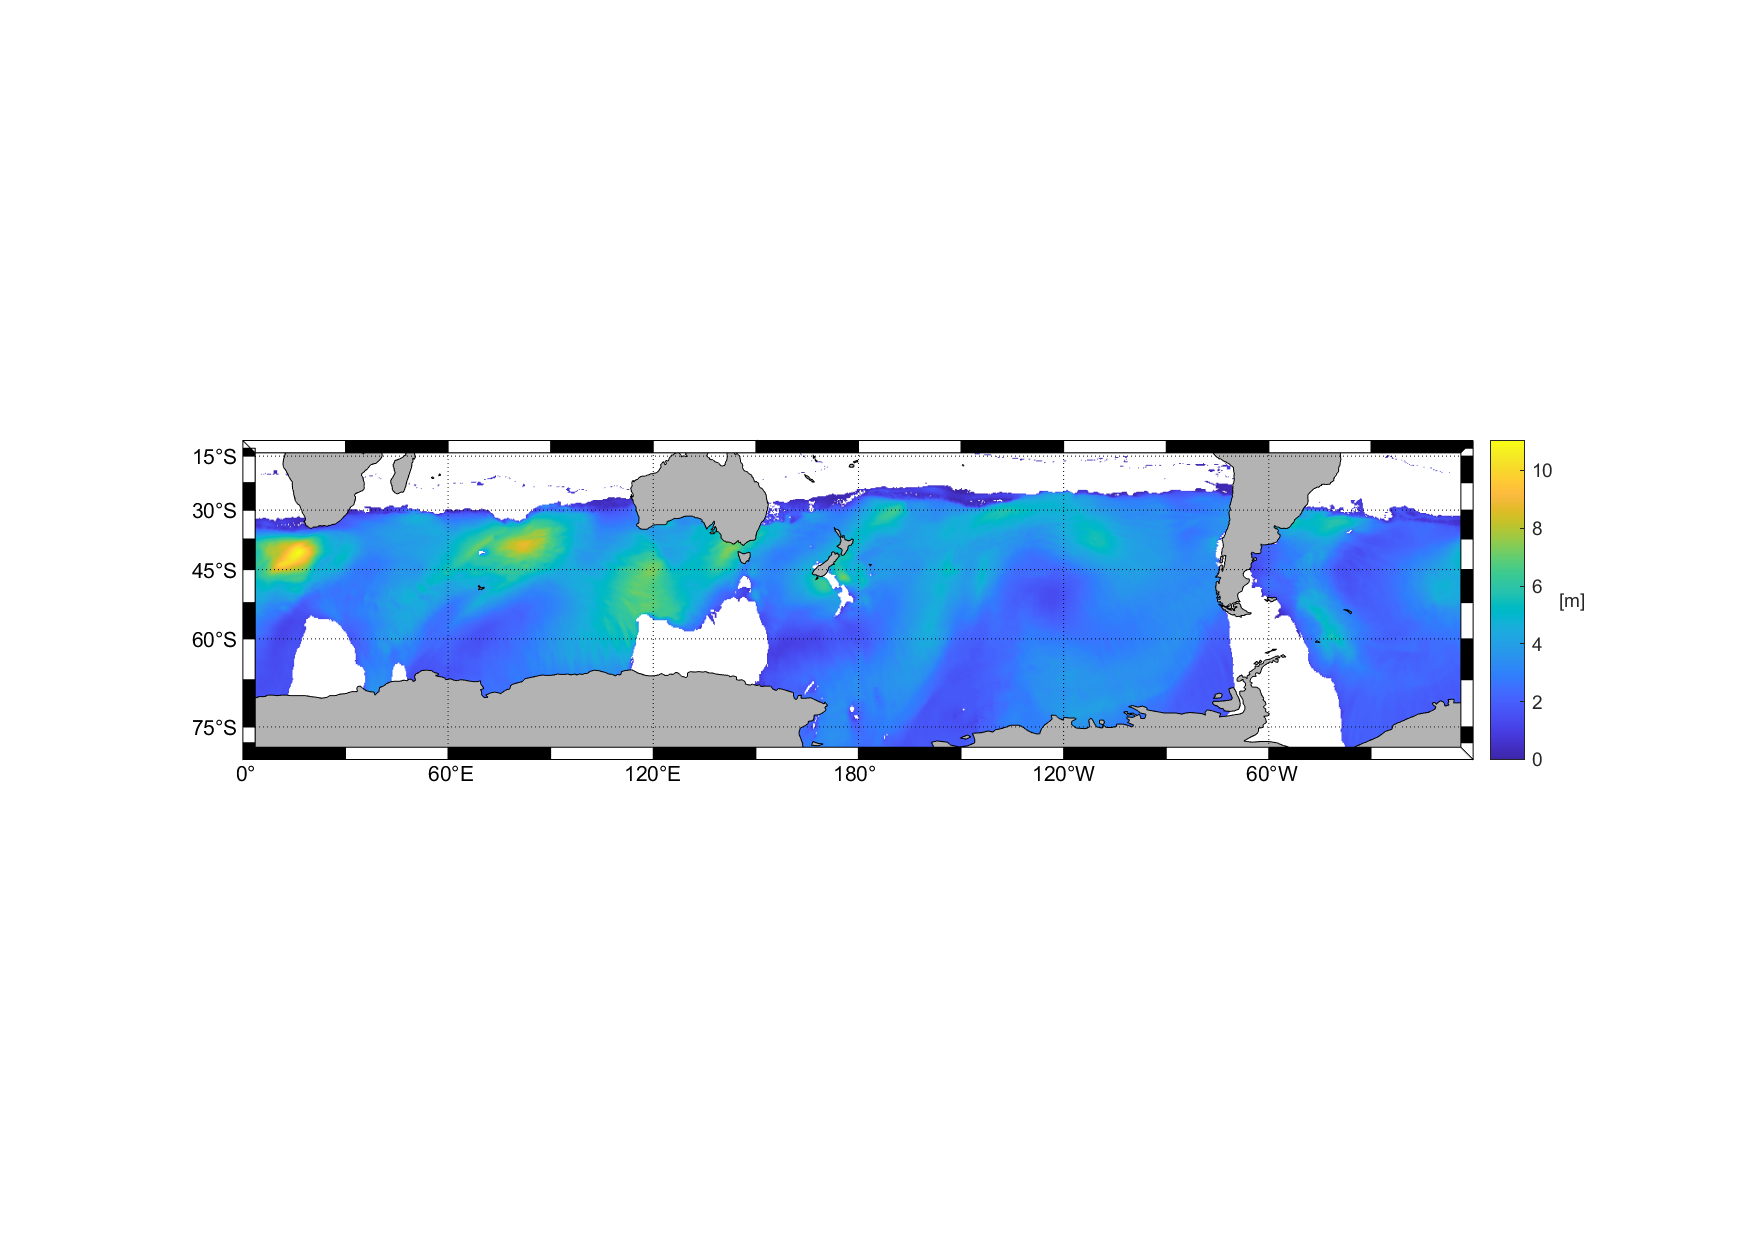
\includegraphics[width=\linewidth]{Figures/PipelineValidation/noaamillersignificantWaveHeight.pdf}
        \caption{Significant wave height.}
        \label{fig:pipelineVal.waveDataPlot.height}
    \end{subfigure}   
    \begin{subfigure}{0.48\linewidth}
        \centering
        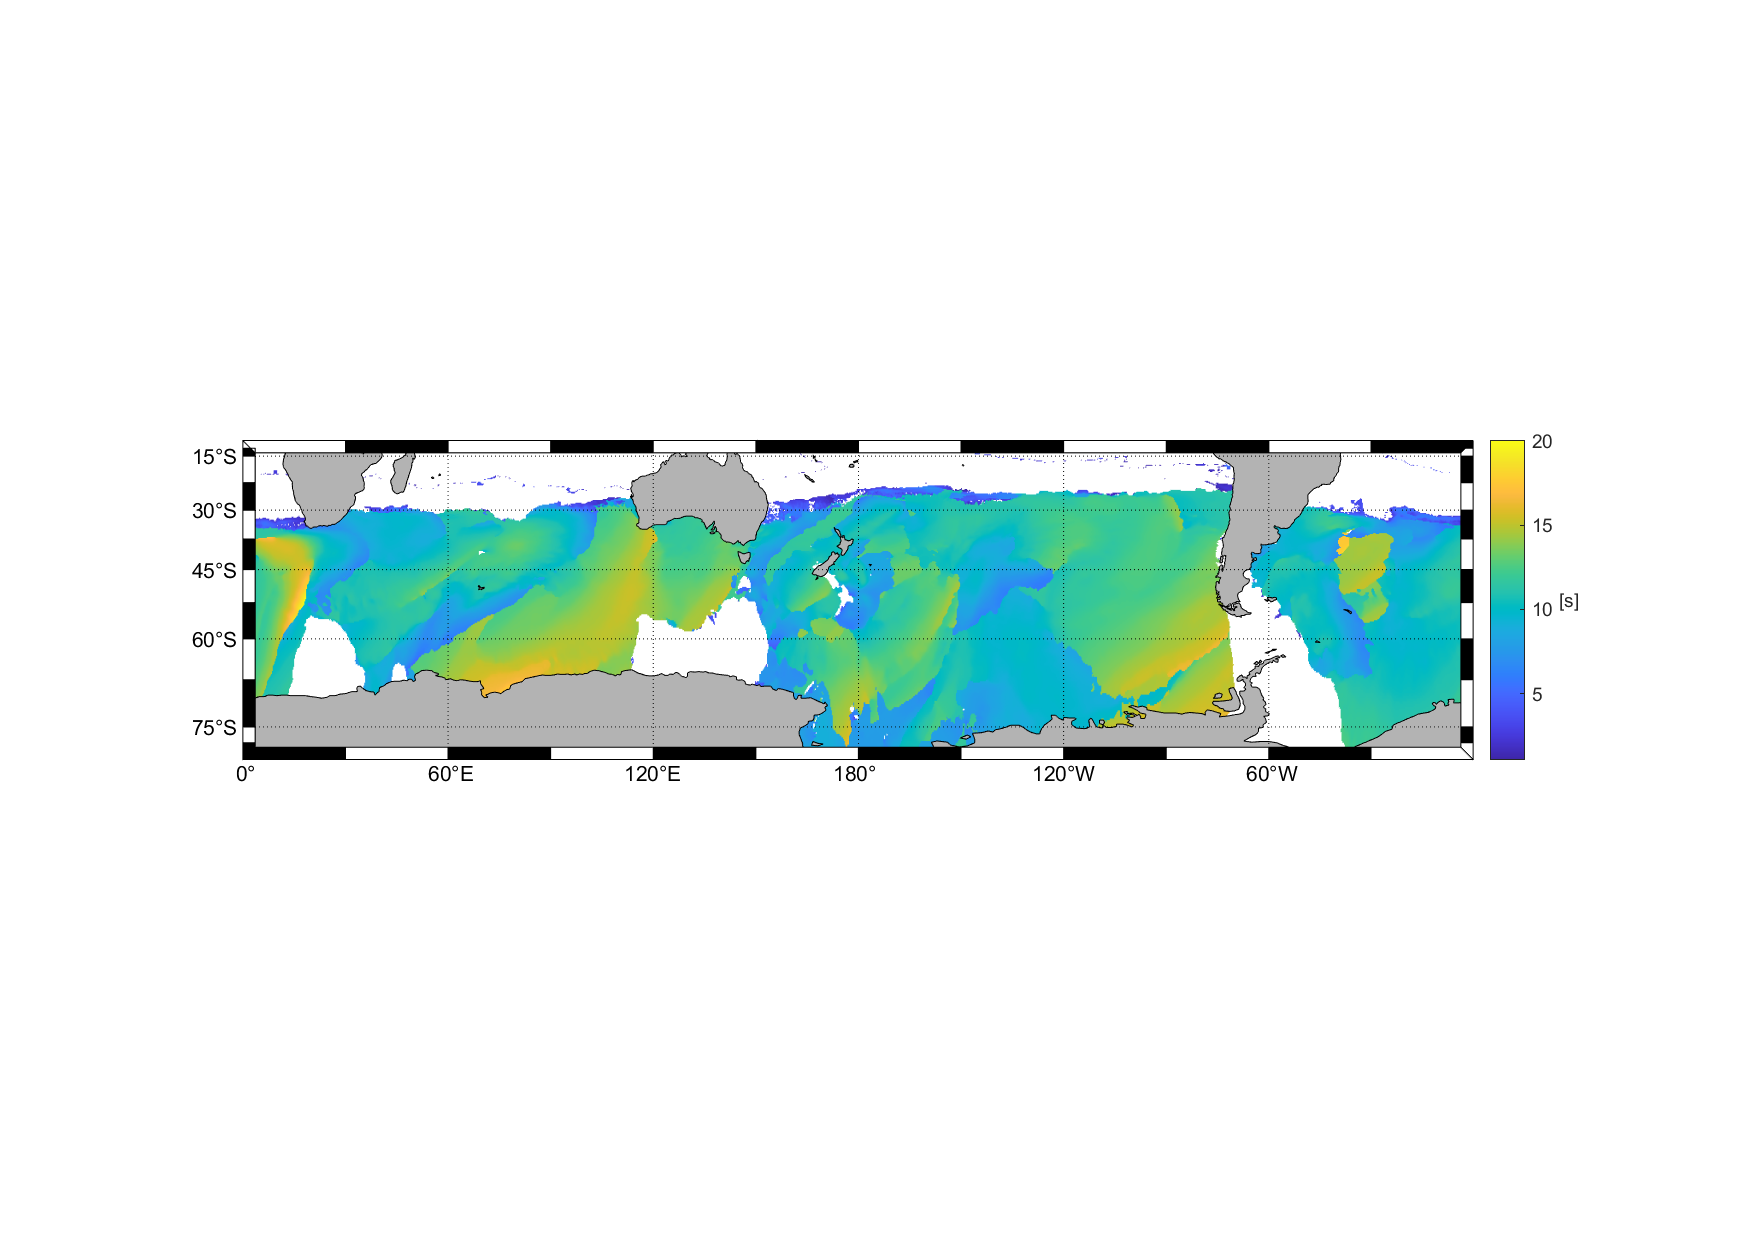
\includegraphics[width=\linewidth]{Figures/PipelineValidation/noaamillersignificantWavePeriod.pdf}
        \caption{Significant wave period.}
        \label{fig:pipelineVal.waveDataPlot.period}
    \end{subfigure}   
    \begin{subfigure}{0.48\linewidth}
        \centering
        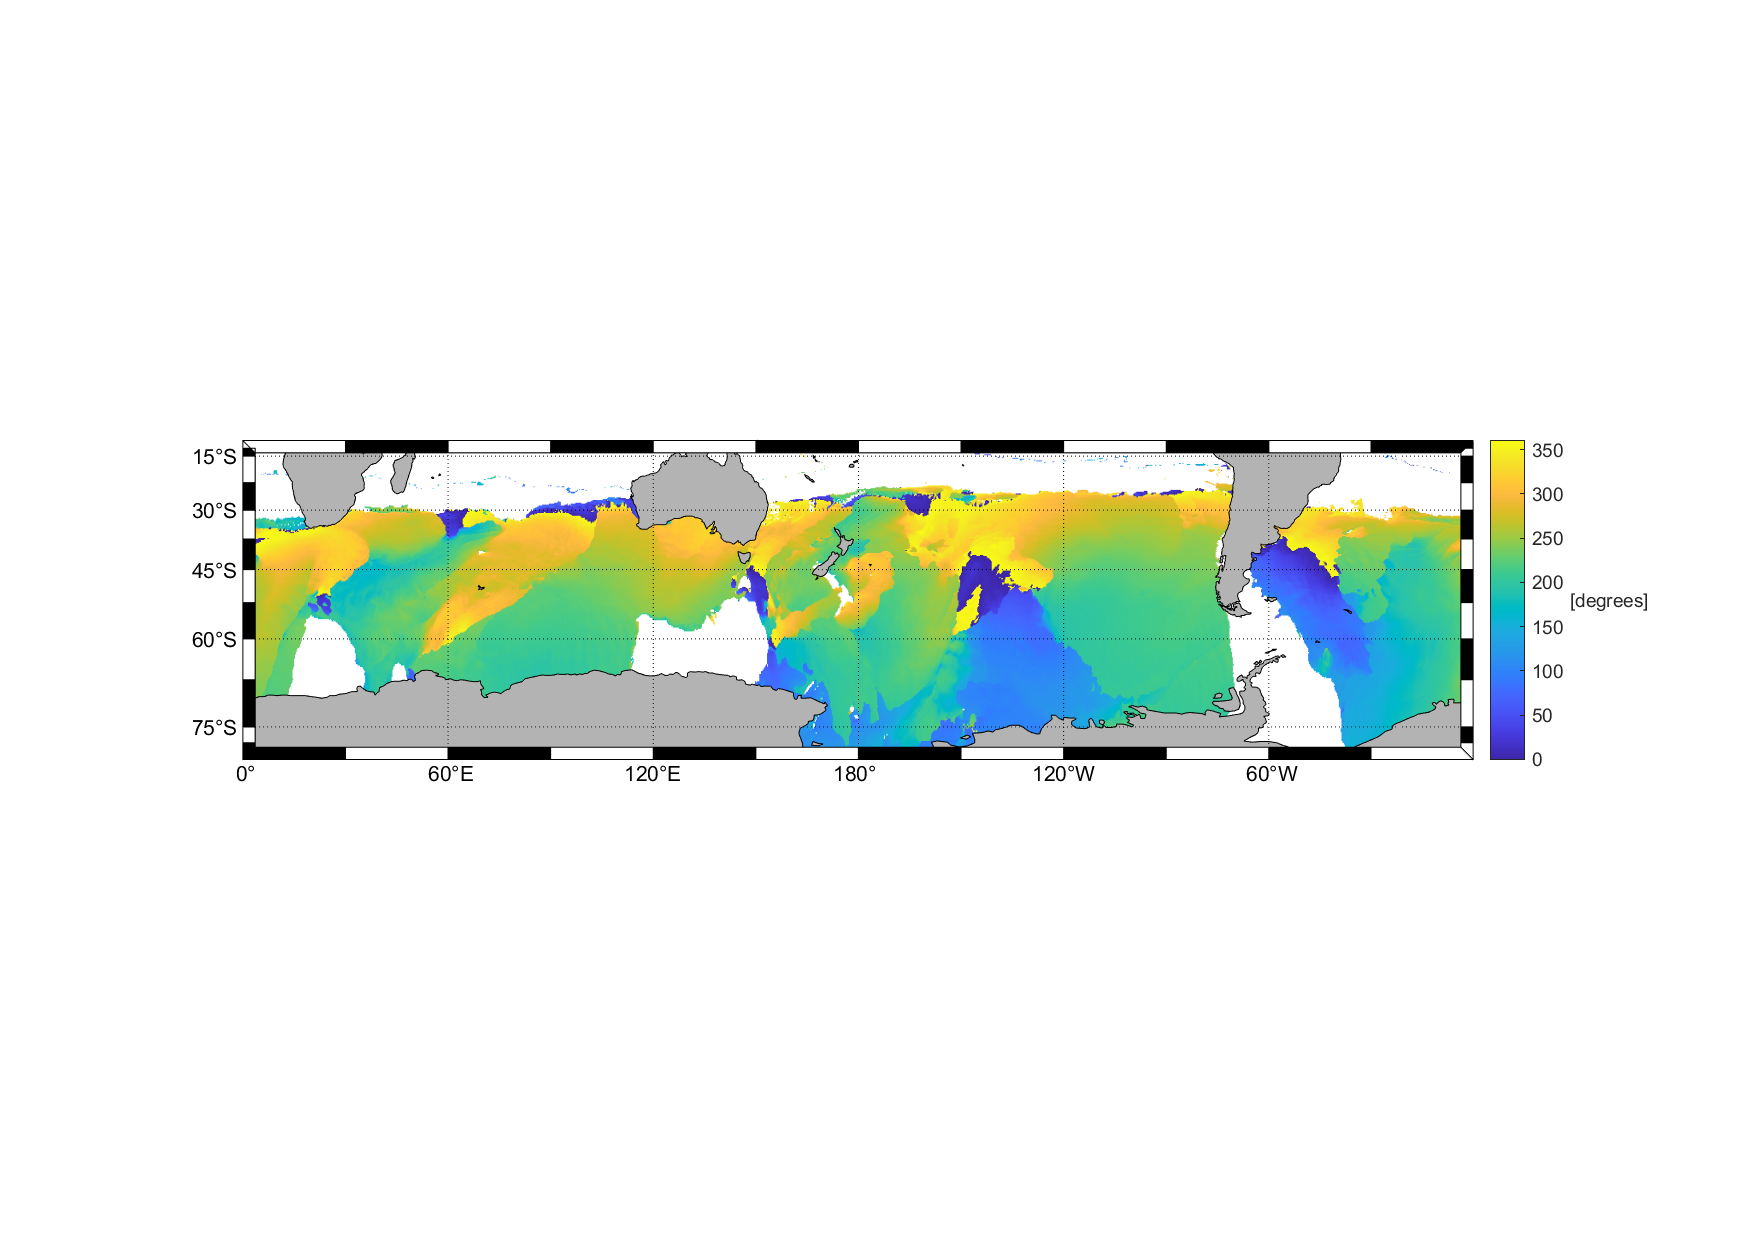
\includegraphics[width=\linewidth]{Figures/PipelineValidation/noaamillerdirection.pdf}
        \caption{Wave direction.}
        \label{fig:pipelineVal.waveDataPlot.direction}
    \end{subfigure}
    \begin{subfigure}{0.48\linewidth}
        \centering
        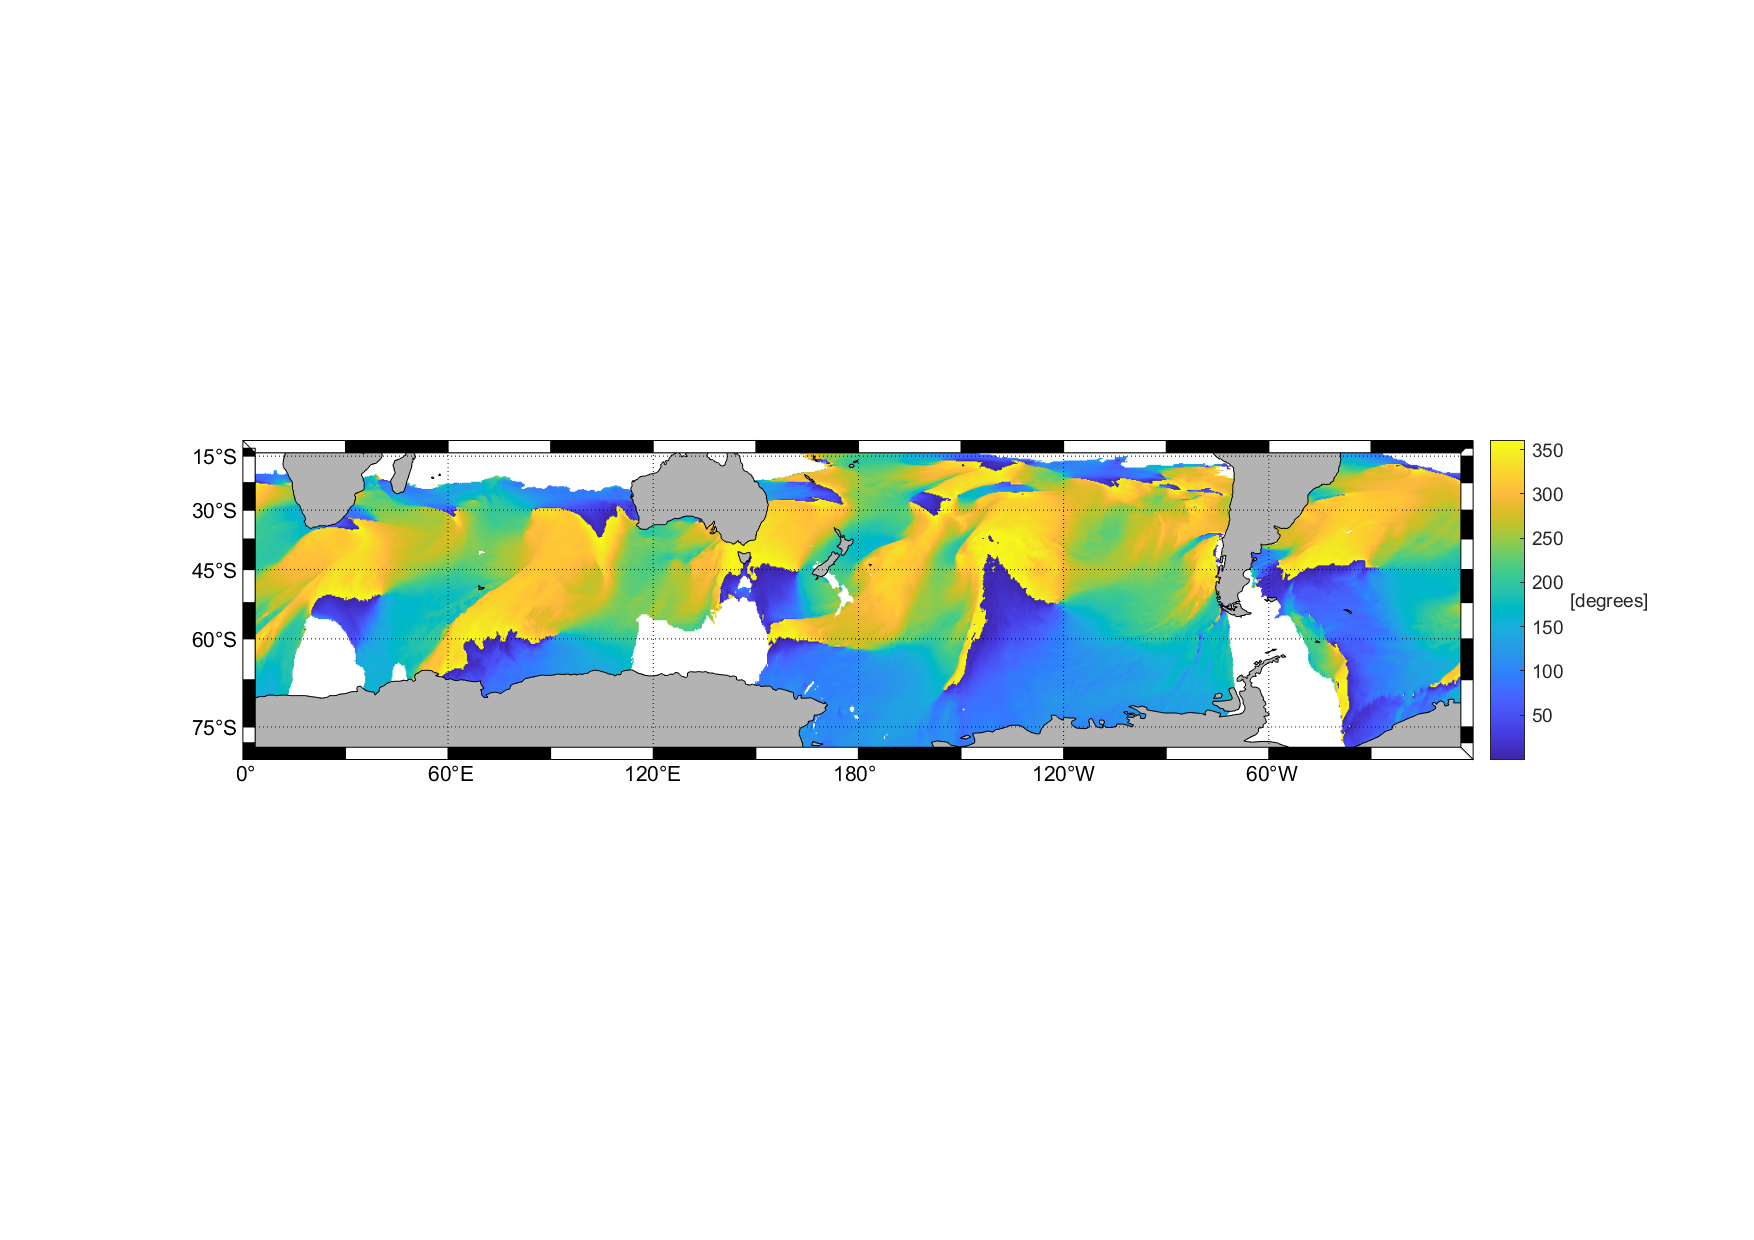
\includegraphics[width=\linewidth]{Figures/PipelineValidation/noaamillerwindDirection.pdf}
        \caption{Wind direction.}
        \label{fig:pipelineVal.waveDataPlot.windDirection}
    \end{subfigure}           
    \begin{subfigure}{0.48\linewidth}
        \centering
        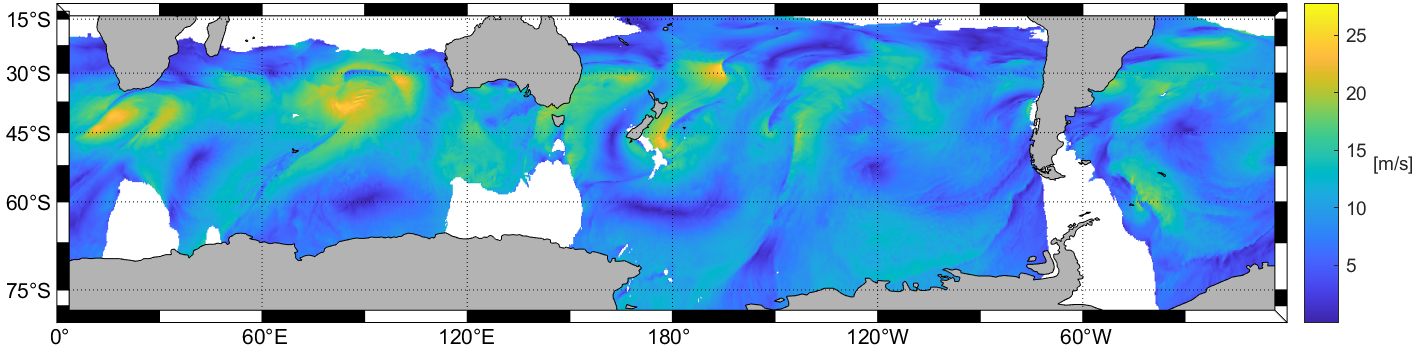
\includegraphics[width=\linewidth]{Figures/PipelineValidation/noaamillerwindSpeed.pdf}
        \caption{Wind speed.}
        \label{fig:pipelineVal.waveDataPlot.windSpeed}
    \end{subfigure}       
    \caption{M\_Map plots using Miller projection of various \acs{ncep} wave data parameters from 02-Oct-2023.}
    \label{fig:pipelineVal.waveDataPlot}
\end{figure}

Figures \ref{fig:pipelineVal.waveDataPlot.direction}, \ref{fig:pipelineVal.waveDataPlot.windDirection} both vary between 0 and 360$\degree$ which verifies that these data are correctly extracted. In terms of agreement within acceptable ranges for Figures \ref{fig:pipelineVal.waveDataPlot.height}, \ref{fig:pipelineVal.waveDataPlot.period}, \ref{fig:pipelineVal.waveDataPlot.windSpeed}, these range of these data makes sense. Therefore, the downloaded \acs{ncep} wave data, as well as both the \href{https://github.com/JNSRYA006/sar-parameter-extraction-pipeline/blob/main/functions/preprocess/get512Transects.m}{\lstinline{downloadNOAAWaveFile}} and \href{https://github.com/JNSRYA006/sar-parameter-extraction-pipeline/blob/main/functions/preprocess/get512Transects.m}{\lstinline{getGribStruct}} functions are implemented correctly.

\subsection{Wave Evolution} \label{subsec:pipelineVal.waveSpectra.waveEvolution}
%% Check holthuisjen expected changes are correct

In order to verify the way in which one-dimensional \acs{jonswap} wave spectra are constructed, it is essential to verify that the expected behaviour of waves when entering shallower water is met. As the depth of water decreases, the peak frequency of the wave is expected to decrease according to Equation \ref{eq:linearWaveTheory.dispersionRelationship.shallowWater}, as an increase in depth increases the $\omega_{peak}$ value. The height of the wave is expected to decrease due to the change in orbital motion of waves due to depth, as detailed in Chapter 5.4.2 of \cite{Holthuijsen2007}. 

To see these changes, geographic coordinates surrounding the Cape Point directional buoy were chosen. These coordinates were generated using the \href{https://github.com/JNSRYA006/sar-parameter-extraction-pipeline/blob/main/functions/waveSpectra/generateSingleJONSWAP.m}{\lstinline{createLatLonGrid}} function and the resulting coordinates are shown in Listing \ref{code:latLonExtract.grid}. However, due to the spatial resolution of 0.25$\degree$ provided by \acs{ncep} wave data, these points are not useful when validating the generation of the wave model. All of the individual points used to generate wave spectra are shown in Figure \ref{fig:pipelineVal.1DWaveSpectrum.map} along with the location of the \acs{csir} directional wave buoy. 

It is important to note that some points in Figure \ref{fig:pipelineVal.1DWaveSpectrum.map} do not aid the verification of generating accurate \acs{jonswap} spectra. The reasons why these are not suitable are discussed in Table \ref{tab:pipelineVal.1DWaveSpectrum.invalidLocs}.

\begin{table}[H]
\centering
\begin{tabular}{|c|c|c|}
\hline
\textbf{Figure \ref{fig:pipelineVal.1DWaveSpectrum.map} Label} & \textbf{Location ($\degree$)} & \textbf{Reason} \\ \hline
WS 1\_3(34S, 18.5E) & 34$\degree$\,S, 18.5$\degree$\,E & \begin{tabular}[c]{@{}c@{}}Data point located on land,\\ as opposed to the ocean.\end{tabular} \\ \hline
WS 2\_3(34.25S, 18.5E) & 34.25$\degree$\,S, 18.5$\degree$\,E & \begin{tabular}[c]{@{}c@{}}Data point located in  False Bay\\ (East of Cape Point), as opposed to being\\ West of Cape Point peninsula.\end{tabular} \\ \hline
WS 3\_3(34.5S, 18.5E) & 34.5$\degree$\,S, 18.5$\degree$\,E & No significant change in depth. \\ \hline
\end{tabular}
\caption{Data points generated by the \href{https://github.com/JNSRYA006/sar-parameter-extraction-pipeline/blob/main/functions/waveSpectra/generateSingleJONSWAP.m}{\lstinline{createLatLonGrid}} function not used to verify wave evolution over space.}
\label{tab:pipelineVal.1DWaveSpectrum.invalidLocs}
\end{table}


% Cite google earth pro and https://www.opendem.info/download_bathymetry.html
% Change labels to include lat and long
\begin{figure}[H]
    \centering
    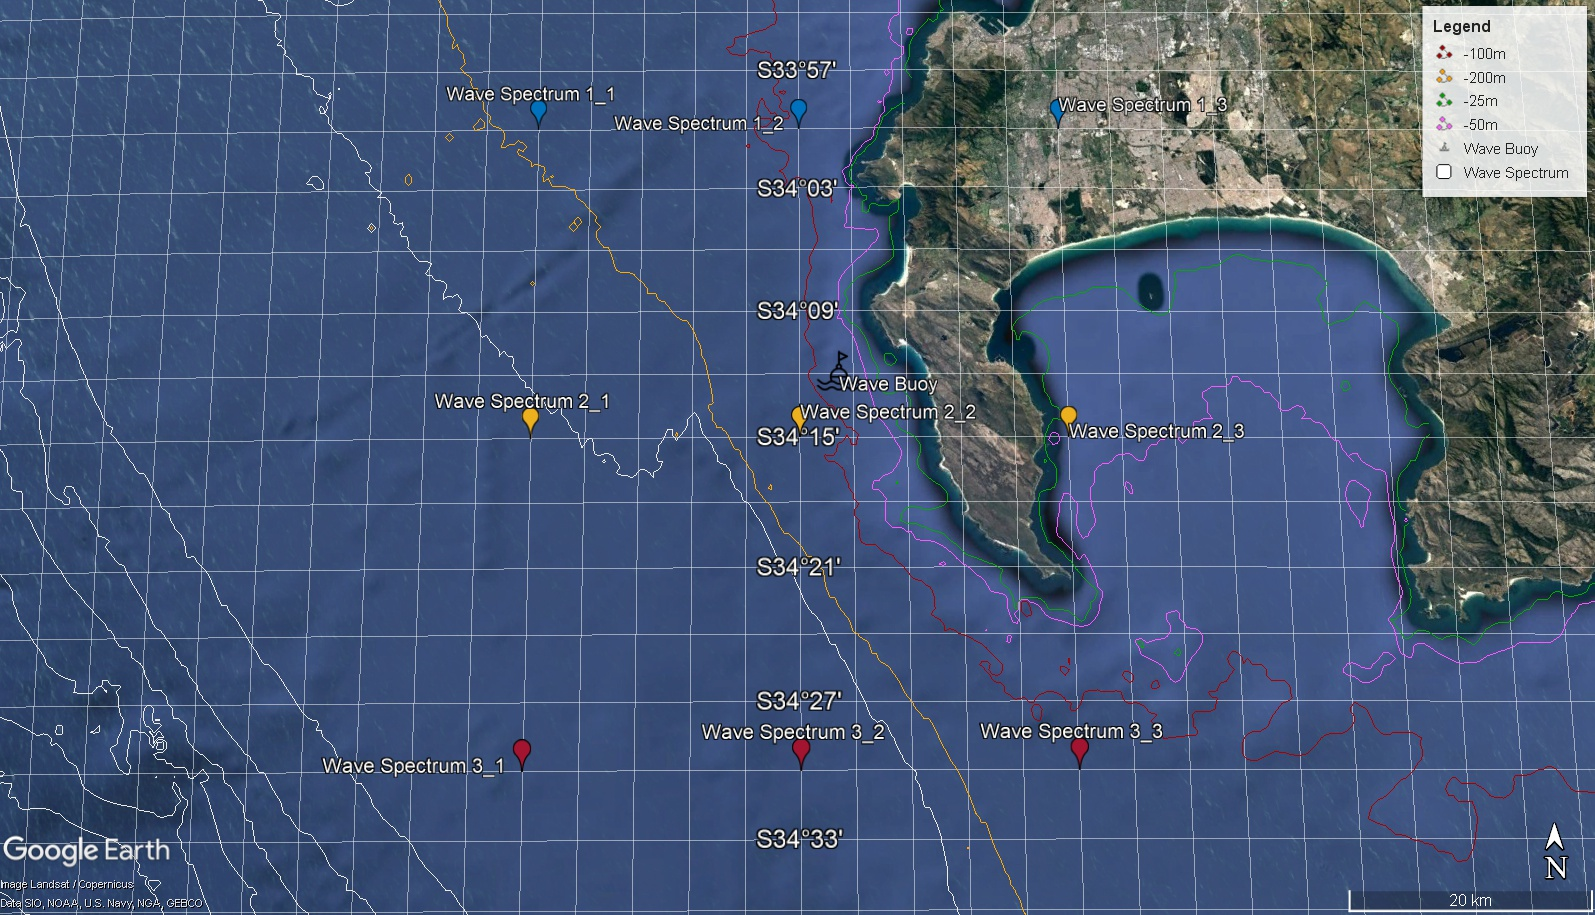
\includegraphics[width=.95\linewidth]{Figures/PipelineValidation/GoogleEarthWaveLocationsContoursGrid.pdf}
    \caption{Geographic points of generated \acs{jonswap} spectra using \acs{ncep} wave data. The location of the \acs{csir} directional wave buoy is shown. The points indicating each wave spectrum location correspond to the colours of the plots generated in Figure \ref{fig:pipelineVal.1DWaveSpectrum.all}. The contours shown in colour represent the respective depths below sea level: \textcolor{25m}{25\,m}, \textcolor{50m}{50\,m}, \textcolor{100m}{100\,m}, \textcolor{200m}{200\,m}, \textcolor{250m}{250\,m}, \textcolor{500m}{500\,m}, and \textcolor{750m}{750\,m}. Bathymetric contour data sourced and adapted from xx.}
    \label{fig:pipelineVal.1DWaveSpectrum.map}
\end{figure}

The wave spectra in Figure \ref{fig:pipelineVal.1DWaveSpectrum.all} can be seen to vary for different geographical locations. Examining each individual plot in Figures \ref{fig:pipelineVal.1DWaveSpectrum.1}, \ref{fig:pipelineVal.1DWaveSpectrum.2}, \ref{fig:pipelineVal.1DWaveSpectrum.3} allows the effect of change in depth to be determined, and verified.

\begin{figure}[H]
    \centering
    \subcaptionbox{\acs{jonswap} spectrum over three distinct latitudes and longitudes obtained from \acs{ncep} wave data. Wave spectra at the same latitude are shown in the same colour whilst the longitude of the wave spectra change.\label{fig:pipelineVal.1DWaveSpectrum.all}}[0.48\linewidth]{
        \resizebox{\linewidth}{!}{% This file was created by matlab2tikz.
%
%The latest updates can be retrieved from
%  http://www.mathworks.com/matlabcentral/fileexchange/22022-matlab2tikz-matlab2tikz
%where you can also make suggestions and rate matlab2tikz.
%
\definecolor{mycolor1}{rgb}{0.00000,0.44706,0.74118}%
\definecolor{mycolor2}{rgb}{0.92941,0.69412,0.12549}%
\definecolor{mycolor3}{rgb}{0.63529,0.07843,0.18431}%
%
\begin{tikzpicture}

\begin{axis}[%
width=4.521in,
height=3.524in,
at={(0.758in,0.523in)},
scale only axis,
unbounded coords=jump,
xmin=0,
xmax=7,
xtick={0,1.5707963267949,3.14159265358979,4.71238898038469,6.28318530717959},
xticklabels={{0},{$\pi\text{/2}$},{$\pi$},{$\text{3}\pi\text{/2}$},{$\text{2}\pi$}},
xlabel style={font=\color{white!15!black}},
xlabel={$\omega\text{ [rad/s]}$},
ymin=0,
ymax=0.07,
ylabel style={font=\color{white!15!black}},
ylabel={$\text{E(}\omega\text{) [m}^\text{2}\text{/rad/Hz]}$},
axis background/.style={fill=white},
axis x line*=bottom,
axis y line*=left,
xmajorgrids,
ymajorgrids,
legend style={legend cell align=left, align=left, draw=white!15!black}
]
\addplot [color=mycolor1]
  table[row sep=crcr]{%
0	nan\\
0.0122958616578857	0\\
0.0245917233157714	0\\
0.0368875849736571	0\\
0.0491834466315427	0\\
0.0614793082894284	0\\
0.0737751699473141	0\\
0.0860710316051998	0\\
0.0983668932630855	0\\
0.110662754920971	0\\
0.122958616578857	0\\
0.135254478236743	0\\
0.147550339894628	0\\
0.159846201552514	0\\
0.1721420632104	0\\
0.184437924868285	0\\
0.196733786526171	0\\
0.209029648184057	0\\
0.221325509841942	0\\
0.233621371499828	0\\
0.245917233157714	0\\
0.258213094815599	0\\
0.270508956473485	0\\
0.282804818131371	0\\
0.295100679789256	0\\
0.307396541447142	0\\
0.319692403105028	0\\
0.331988264762914	0\\
0.344284126420799	0\\
0.356579988078685	0\\
0.368875849736571	0\\
0.381171711394456	0\\
0.393467573052342	3.34419642251927e-289\\
0.405763434710228	1.28025550684515e-255\\
0.418059296368113	9.09801077678118e-227\\
0.430355158025999	7.17955661273785e-202\\
0.442651019683885	2.69655368843393e-180\\
0.45494688134177	1.58628012010437e-161\\
0.467242742999656	3.89542970829007e-145\\
0.479538604657542	8.98638404577865e-131\\
0.491834466315427	3.82270042312654e-118\\
0.504130327973313	5.26770583144193e-107\\
0.516426189631199	3.77319584880466e-97\\
0.528722051289085	2.09280440992325e-88\\
0.54101791294697	1.25940961397226e-80\\
0.553313774604856	1.09515982022289e-73\\
0.565609636262742	1.75705762280086e-67\\
0.577905497920627	6.41078704598093e-62\\
0.590201359578513	6.36556541298869e-57\\
0.602497221236399	2.00790222716586e-52\\
0.614793082894284	2.29975120115565e-48\\
0.62708894455217	1.0739089812567e-44\\
0.639384806210056	2.2611897369356e-41\\
0.651680667867941	2.34373434790845e-38\\
0.663976529525827	1.29120102064113e-35\\
0.676272391183713	4.04370246086255e-33\\
0.688568252841599	7.63655457505185e-31\\
0.700864114499484	9.16040465793229e-29\\
0.71315997615737	7.30704687792533e-27\\
0.725455837815256	4.03632650075498e-25\\
0.737751699473141	1.60048122856397e-23\\
0.750047561131027	4.70315840849396e-22\\
0.762343422788913	1.05373259129103e-20\\
0.774639284446798	1.84612768297031e-19\\
0.786935146104684	2.58700579350983e-18\\
0.79923100776257	2.95881393535563e-17\\
0.811526869420455	2.81249420426715e-16\\
0.823822731078341	2.25831112879919e-15\\
0.836118592736227	1.55434141155284e-14\\
0.848414454394112	9.29181663406122e-14\\
0.860710316051998	4.88210181401567e-13\\
0.873006177709884	2.27890731963973e-12\\
0.88530203936777	9.54283210921378e-12\\
0.897597901025655	3.61642202927237e-11\\
0.909893762683541	1.25025283956853e-10\\
0.922189624341426	3.97174755431221e-10\\
0.934485485999312	1.16706162830048e-09\\
0.946781347657198	3.19111067187954e-09\\
0.959077209315084	8.16400766983196e-09\\
0.971373070972969	1.9640330585374e-08\\
0.983668932630855	4.46335695515399e-08\\
0.995964794288741	9.62181033753792e-08\\
1.00826065594663	1.97513463595782e-07\\
1.02055651760451	3.87441107221251e-07\\
1.0328523792624	7.28589610711906e-07\\
1.04514824092028	1.31738947970889e-06\\
1.05744410257817	2.2965814013734e-06\\
1.06973996423605	3.86967598098188e-06\\
1.08203582589394	6.3167793390538e-06\\
1.09433168755183	1.00108401330565e-05\\
1.10662754920971	1.54331073387638e-05\\
1.1189234108676	2.31864186076149e-05\\
1.13121927252548	3.40048987204158e-05\\
1.14351513418337	4.8758751783582e-05\\
1.15581099584125	6.84530749027877e-05\\
1.16810685749914	9.4219982204407e-05\\
1.18040271915703	0.000127303769055645\\
1.19269858081491	0.000169039321722978\\
1.2049944424728	0.000220824440487555\\
1.21729030413068	0.000284087151892057\\
1.22958616578857	0.000360249404979067\\
1.24188202744645	0.000450688755701355\\
1.25417788910434	0.000556699734546854\\
1.26647375076223	0.000679456568201386\\
1.27876961242011	0.000819978800037321\\
1.291065474078	0.000979101146719596\\
1.30336133573588	0.00115744866365773\\
1.31565719739377	0.00135541799595638\\
1.32795305905165	0.00157316518818653\\
1.34024892070954	0.00181060023680969\\
1.35254478236743	0.00206738831012199\\
1.36484064402531	0.0023429573437477\\
1.3771365056832	0.0026365115513501\\
1.38943236734108	0.00294705027163909\\
1.40172822899897	0.00327339150067656\\
1.41402409065685	0.00361419942578141\\
1.42631995231474	0.00396801527386398\\
1.43861581397263	0.00433329080057555\\
1.45091167563051	0.00470842376409372\\
1.4632075372884	0.00509179473579552\\
1.47550339894628	0.00548180458817485\\
1.48779926060417	0.00587691195971112\\
1.50009512226205	0.00627566992269608\\
1.51239098391994	0.0066767609741115\\
1.52468684557783	0.00707902933805387\\
1.53698270723571	0.0074815094231008\\
1.5492785688936	0.00788344913644478\\
1.56157443055148	0.00828432663895199\\
1.57387029220937	0.00868385905314233\\
1.58616615386725	0.00908200162993884\\
1.59846201552514	0.00947893595725699\\
1.61075787718303	0.00987504596704363\\
1.62305373884091	0.0102708807757592\\
1.6353496004988	0.0106671037820176\\
1.64764546215668	0.0110644279490677\\
1.65994132381457	0.0114635378260619\\
1.67223718547245	0.0118649996213497\\
1.68453304713034	0.0122691615466052\\
1.69682890878822	0.0126760477126327\\
1.70912477044611	0.0130852500723398\\
1.721420632104	0.0134958242396934\\
1.73371649376188	0.0139061963823064\\
1.74601235541977	0.0143140896395624\\
1.75830821707765	0.0147164794313437\\
1.77060407873554	0.015109587298661\\
1.78289994039342	0.0154889222233254\\
1.79519580205131	0.0158493763991941\\
1.8074916637092	0.0161853789730349\\
1.81978752536708	0.016491106350086\\
1.83208338702497	0.0167607415774144\\
1.84437924868285	0.0169887687258095\\
1.85667511034074	0.0171702820380385\\
1.86897097199862	0.0173012850143819\\
1.88126683365651	0.0173789526276866\\
1.8935626953144	0.0174018877913857\\
1.90585855697228	0.0173792516945915\\
1.91815441863017	0.0173187030448506\\
1.93045028028805	0.0172218404888346\\
1.94274614194594	0.0170907927342484\\
1.95504200360382	0.0169281498507053\\
1.96733786526171	0.016736879485734\\
1.9796337269196	0.0165202329326319\\
1.99192958857748	0.0162816462986226\\
2.00422545023537	0.0160246419065975\\
2.01652131189325	0.0157527345731798\\
2.02881717355114	0.0154693466262642\\
2.04111303520902	0.015177734562442\\
2.05340889686691	0.0148809292085418\\
2.0657047585248	0.0145816902415667\\
2.07800062018268	0.0142824750172383\\
2.09029648184057	0.0139854209133983\\
2.10259234349845	0.0136923398385474\\
2.11488820515634	0.013404723192043\\
2.12718406681422	0.0131237553765477\\
2.13947992847211	0.012850333928277\\
2.15177579012999	0.012585094413024\\
2.16407165178788	0.0123284384010557\\
2.17636751344577	0.0120805630495126\\
2.18866337510365	0.0118414910596127\\
2.20095923676154	0.0116111000165573\\
2.21325509841942	0.0113891503476316\\
2.22555096007731	0.0111753113392689\\
2.2378468217352	0.0109691848321502\\
2.25014268339308	0.0107703263635373\\
2.26243854505097	0.0105782636491412\\
2.27473440670885	0.0103925123954185\\
2.28703026836674	0.0102125895103747\\
2.29932613002462	0.0100380238399035\\
2.31162199168251	0.00986836460031791\\
2.3239178533404	0.00970318770850608\\
2.33621371499828	0.00954210023112282\\
2.34850957665617	0.00938474318504906\\
2.36080543831405	0.00923079292435986\\
2.37310129997194	0.00907996134539838\\
2.38539716162982	0.00893199513229698\\
2.39769302328771	0.00878667425142768\\
2.40998888494559	0.0086438098857951\\
2.42228474660348	0.00850324198030174\\
2.43458060826137	0.0083648365470924\\
2.44687646991925	0.00822848285775266\\
2.45917233157714	0.00809409062684347\\
2.47146819323502	0.00796158726983848\\
2.48376405489291	0.00783091529859396\\
2.49605991655079	0.00770202989947307\\
2.50835577820868	0.00757489672346623\\
2.52065163986657	0.00744948990424842\\
2.53294750152445	0.00732579030911486\\
2.54524336318234	0.00720378401905237\\
2.55753922484022	0.00708346102766523\\
2.56983508649811	0.00696481414405219\\
2.58213094815599	0.0068478380817634\\
2.59442680981388	0.00673252871437512\\
2.60672267147177	0.00661888247773352\\
2.61901853312965	0.00650689589927961\\
2.63131439478754	0.00639656523584554\\
2.64361025644542	0.00628788620270682\\
2.65590611810331	0.00618085377832044\\
2.66820197976119	0.00607546207094004\\
2.68049784141908	0.0059717042350745\\
2.69279370307697	0.00586957242746926\\
2.70508956473485	0.0057690577938902\\
2.71738542639274	0.00567015047944444\\
2.72968128805062	0.00557283965646651\\
2.74197714970851	0.0054771135651265\\
2.75427301136639	0.00538295956288353\\
2.76656887302428	0.00529036417972385\\
2.77886473468217	0.00519931317680114\\
2.79116059634005	0.00510979160665305\\
2.80345645799794	0.00502178387361852\\
2.81575231965582	0.00493527379344081\\
2.82804818131371	0.0048502446513258\\
2.84034404297159	0.0047666792579471\\
2.85263990462948	0.00468456000306085\\
2.86493576628737	0.00460386890652315\\
2.87723162794525	0.00452458766660076\\
2.88952748960314	0.0044466977055378\\
2.90182335126102	0.00437018021239355\\
2.91411921291891	0.00429501618320338\\
2.92641507457679	0.00422118645854048\\
2.93871093623468	0.00414867175857284\\
2.95100679789256	0.00407745271572042\\
2.96330265955045	0.00400750990502326\\
2.97559852120834	0.00393882387233332\\
2.98789438286622	0.00387137516044325\\
3.00019024452411	0.00380514433326318\\
3.01248610618199	0.0037401119981539\\
3.02478196783988	0.00367625882652118\\
3.03707782949776	0.00361356557277201\\
3.04937369115565	0.00355201309172901\\
3.06166955281354	0.0034915823545951\\
3.07396541447142	0.00343225446355593\\
3.08626127612931	0.00337401066510325\\
3.09855713778719	0.00331683236215819\\
3.11085299944508	0.00326070112506917\\
3.12314886110296	0.00320559870155528\\
3.13544472276085	0.00315150702566218\\
3.14774058441874	0.00309840822579381\\
3.16003644607662	0.0030462846318797\\
3.17233230773451	0.00299511878173458\\
3.18462816939239	0.00294489342666344\\
3.19692403105028	0.00289559153636255\\
3.20921989270816	0.00284719630316386\\
3.22151575436605	0.00279969114566754\\
3.23381161602394	0.00275305971180489\\
3.24610747768182	0.00270728588137131\\
3.25840333933971	0.00266235376806688\\
3.27069920099759	0.00261824772107962\\
3.28299506265548	0.0025749523262447\\
3.29529092431336	0.00253245240681082\\
3.30758678597125	0.00249073302384293\\
3.31988264762914	0.00244977947628899\\
3.33217850928702	0.00240957730073666\\
3.34447437094491	0.00237011227088411\\
3.35677023260279	0.00233137039674796\\
3.36906609426068	0.0022933379236296\\
3.38136195591856	0.00225600133086013\\
3.39365781757645	0.00221934733034266\\
3.40595367923434	0.00218336286490959\\
3.41824954089222	0.00214803510651163\\
3.43054540255011	0.00211335145425364\\
3.44284126420799	0.00207929953229227\\
3.45513712586588	0.00204586718760842\\
3.46743298752376	0.00201304248766768\\
3.47972884918165	0.00198081371798019\\
3.49202471083954	0.00194916937957116\\
3.50432057249742	0.00191809818637236\\
3.51661643415531	0.00188758906254403\\
3.52891229581319	0.0018576311397364\\
3.54120815747108	0.00182821375429893\\
3.55350401912896	0.00179932644444514\\
3.56579988078685	0.00177095894738025\\
3.57809574244473	0.00174310119639827\\
3.59039160410262	0.00171574331795476\\
3.60268746576051	0.0016888756287211\\
3.61498332741839	0.00166248863262545\\
3.62727918907628	0.00163657301788557\\
3.63957505073416	0.00161111965403773\\
3.65187091239205	0.0015861195889663\\
3.66416677404994	0.00156156404593756\\
3.67646263570782	0.00153744442064151\\
3.68875849736571	0.00151375227824485\\
3.70105435902359	0.00149047935045825\\
3.71335022068148	0.00146761753262046\\
3.72564608233936	0.00144515888080198\\
3.73794194399725	0.00142309560893049\\
3.75023780565513	0.00140142008594007\\
3.76253366731302	0.00138012483294616\\
3.77482952897091	0.00135920252044798\\
3.78712539062879	0.00133864596555986\\
3.79942125228668	0.00131844812927288\\
3.81171711394456	0.00129860211374814\\
3.82401297560245	0.00127910115964251\\
3.83630883726033	0.00125993864346814\\
3.84860469891822	0.00124110807498621\\
3.86090056057611	0.00122260309463597\\
3.87319642223399	0.00120441747099944\\
3.88549228389188	0.00118654509830238\\
3.89778814554976	0.00116897999395205\\
3.91008400720765	0.00115171629611195\\
3.92237986886553	0.00113474826131388\\
3.93467573052342	0.00111807026210761\\
3.94697159218131	0.00110167678474807\\
3.95926745383919	0.00108556242692043\\
3.97156331549708	0.00106972189550273\\
3.98385917715496	0.00105415000436641\\
3.99615503881285	0.00103884167221433\\
4.00845090047073	0.00102379192045631\\
4.02074676212862	0.00100899587112205\\
4.03304262378651	0.000994448744811049\\
4.04533848544439	0.000980145858679543\\
4.05763434710228	0.000966082624463944\\
4.06993020876016	0.000952254546540628\\
4.08222607041805	0.000938657220021713\\
4.09452193207593	0.000925286328886466\\
4.10681779373382	0.00091213764414798\\
4.1191136553917	0.000899207022054753\\
4.13140951704959	0.000886490402326741\\
4.14370537870748	0.000873983806425488\\
4.15600124036536	0.000861683335857888\\
4.16829710202325	0.000849585170513158\\
4.18059296368113	0.000837685567032558\\
4.19288882533902	0.000825980857211403\\
4.2051846869969	0.0008144674464329\\
4.21748054865479	0.000803141812133341\\
4.22977641031268	0.000792000502298181\\
4.24207227197056	0.000781040133988504\\
4.25436813362845	0.000770257391897421\\
4.26666399528633	0.00075964902693588\\
4.27895985694422	0.000749211854847443\\
4.29125571860211	0.000738942754851508\\
4.30355158025999	0.000728838668314515\\
4.31584744191788	0.000718896597448629\\
4.32814330357576	0.000709113604037451\\
4.34043916523365	0.00069948680818823\\
4.35273502689153	0.000690013387110138\\
4.36503088854942	0.000680690573918113\\
4.37732675020731	0.000671515656461793\\
4.38962261186519	0.000662485976179102\\
4.40191847352308	0.000653598926973972\\
4.41421433518096	0.000644851954117806\\
4.42651019683885	0.000636242553174168\\
4.43880605849673	0.000627768268946294\\
4.45110192015462	0.000619426694446945\\
4.46339778181251	0.000611215469890196\\
4.47569364347039	0.000603132281704698\\
4.48798950512828	0.000595174861568003\\
4.50028536678616	0.000587340985461523\\
4.51258122844405	0.000579628472745707\\
4.52487709010193	0.000572035185255035\\
4.53717295175982	0.000564559026412404\\
4.5494688134177	0.000557197940362531\\
4.56176467507559	0.00054994991112397\\
4.57406053673348	0.000542812961759361\\
4.58635639839136	0.000535785153563524\\
4.59865226004925	0.000528864585269042\\
4.61094812170713	0.00052204939226895\\
4.62324398336502	0.000515337745856178\\
4.6355398450229	0.000508727852479397\\
4.64783570668079	0.000502217953014912\\
4.66013156833868	0.000495806322054271\\
4.67242742999656	0.000489491267207245\\
4.68472329165445	0.00048327112841986\\
4.69701915331233	0.000477144277307152\\
4.70931501497022	0.000471109116500332\\
4.7216108766281	0.000465164079008043\\
4.73390673828599	0.000459307627591423\\
4.74620259994388	0.000453538254152655\\
4.75849846160176	0.000447854479136719\\
4.77079432325965	0.000442254850946066\\
4.78309018491753	0.000436737945367922\\
4.79538604657542	0.000431302365013958\\
4.8076819082333	0.000425946738772039\\
4.81997776989119	0.000420669721269815\\
4.83227363154908	0.00041546999234986\\
4.84456949320696	0.00041034625655614\\
4.85686535486485	0.000405297242631535\\
4.86916121652273	0.000400321703026189\\
4.88145707818062	0.000395418413416441\\
4.8937529398385	0.000390586172234104\\
4.90604880149639	0.000385823800205873\\
4.91834466315427	0.000381130139902625\\
4.93064052481216	0.000376504055298402\\
4.94293638647005	0.000371944431338866\\
4.95523224812793	0.000367450173519001\\
4.96752810978582	0.000363020207469875\\
4.9798239714437	0.000358653478554253\\
4.99211983310159	0.000354348951470867\\
5.00441569475948	0.000350105609867147\\
5.01671155641736	0.000345922455960234\\
5.02900741807525	0.000341798510166082\\
5.04130327973313	0.000337732810736479\\
5.05359914139102	0.000333724413403804\\
5.0658950030489	0.000329772391033349\\
5.07819086470679	0.000325875833283049\\
5.09048672636467	0.000322033846270436\\
5.10278258802256	0.000318245552246677\\
5.11507844968045	0.000314510089277526\\
5.12737431133833	0.00031082661093104\\
5.13967017299622	0.000307194285971914\\
5.1519660346541	0.000303612298062282\\
5.16426189631199	0.000300079845468837\\
5.17655775796987	0.000296596140776148\\
5.18885361962776	0.000293160410606011\\
5.20114948128565	0.000289771895342729\\
5.21344534294353	0.000286429848864156\\
5.22574120460142	0.000283133538278418\\
5.2380370662593	0.000279882243666143\\
5.25033292791719	0.000276675257828116\\
5.26262878957507	0.000273511886038206\\
5.27492465123296	0.000270391445801484\\
5.28722051289085	0.000267313266617378\\
5.29951637454873	0.000264276689747787\\
5.31181223620662	0.000261281067990028\\
5.3241080978645	0.00025832576545451\\
5.33640395952239	0.000255410157347042\\
5.34869982118027	0.000252533629755657\\
5.36099568283816	0.000249695579441861\\
5.37329154449605	0.000246895413636219\\
5.38558740615393	0.00024413254983816\\
5.39788326781182	0.000241406415619933\\
5.4101791294697	0.000238716448434603\\
5.42247499112759	0.000236062095428015\\
5.43477085278547	0.000233442813254624\\
5.44706671444336	0.000230858067897119\\
5.45936257610125	0.00022830733448975\\
5.47165843775913	0.000225790097145283\\
5.48395429941702	0.000223305848785494\\
5.4962501610749	0.000220854090975143\\
5.50854602273279	0.000218434333759326\\
5.52084188439067	0.000216046095504163\\
5.53313774604856	0.000213688902740717\\
5.54543360770645	0.000211362290012102\\
5.55772946936433	0.000209065799723692\\
5.57002533102222	0.000206798981996369\\
5.5823211926801	0.000204561394522753\\
5.59461705433799	0.000202352602426333\\
5.60691291599587	0.000200172178123454\\
5.61920877765376	0.000198019701188079\\
5.63150463931164	0.000195894758219287\\
5.64380050096953	0.000193796942711433\\
5.65609636262742	0.000191725854926917\\
5.6683922242853	0.00018968110177151\\
5.68068808594319	0.000187662296672171\\
5.69298394760107	0.000185669059457322\\
5.70527980925896	0.000183701016239501\\
5.71757567091684	0.000181757799300367\\
5.72987153257473	0.000179839046977991\\
5.74216739423262	0.000177944403556393\\
5.7544632558905	0.000176073519157269\\
5.76675911754839	0.000174226049633875\\
5.77905497920627	0.000172401656466997\\
5.79135084086416	0.000170600006662997\\
5.80364670252204	0.000168820772653861\\
5.81594256417993	0.000167063632199222\\
5.82823842583782	0.000165328268290312\\
5.8405342874957	0.000163614369055801\\
5.85283014915359	0.000161921627669489\\
5.86512601081147	0.000160249742259805\\
5.87742187246936	0.000158598415821073\\
5.88971773412724	0.000156967356126522\\
5.90201359578513	0.000155356275642989\\
5.91430945744302	0.000153764891447277\\
5.9266053191009	0.000152192925144158\\
5.93890118075879	0.000150640102785949\\
5.95119704241667	0.000149106154793665\\
5.96349290407456	0.000147590815879686\\
5.97578876573244	0.000146093824971931\\
5.98808462739033	0.000144614925139487\\
6.00038048904822	0.000143153863519677\\
6.0126763507061	0.000141710391246535\\
6.02497221236399	0.000140284263380646\\
6.03726807402187	0.000138875238840341\\
6.04956393567976	0.000137483080334212\\
6.06185979733764	0.000136107554294908\\
6.07415565899553	0.000134748430814209\\
6.08645152065342	0.000133405483579327\\
6.0987473823113	0.000132078489810429\\
6.11104324396919	0.000130767230199341\\
6.12333910562707	0.000129471488849426\\
6.13563496728496	0.000128191053216586\\
6.14793082894284	0.0001269257140514\\
6.16022669060073	0.000125675265342338\\
6.17252255225862	0.000124439504260058\\
6.1848184139165	0.000123218231102752\\
6.19711427557439	0.000122011249242511\\
6.20941013723227	0.000120818365072709\\
6.22170599889016	0.000119639387956367\\
6.23400186054804	0.000118474130175486\\
6.24629772220593	0.000117322406881326\\
6.25859358386381	0.000116184036045615\\
6.2708894455217	0.000115058838412668\\
6.28318530717959	0.000113946637452394\\
};
\addlegendentry{-34S, 18E}

\addplot [color=mycolor1]
  table[row sep=crcr]{%
0	nan\\
0.0122958616578857	0\\
0.0245917233157714	0\\
0.0368875849736571	0\\
0.0491834466315427	0\\
0.0614793082894284	0\\
0.0737751699473141	0\\
0.0860710316051998	0\\
0.0983668932630855	0\\
0.110662754920971	0\\
0.122958616578857	0\\
0.135254478236743	0\\
0.147550339894628	0\\
0.159846201552514	0\\
0.1721420632104	0\\
0.184437924868285	0\\
0.196733786526171	0\\
0.209029648184057	0\\
0.221325509841942	0\\
0.233621371499828	0\\
0.245917233157714	0\\
0.258213094815599	0\\
0.270508956473485	0\\
0.282804818131371	0\\
0.295100679789256	0\\
0.307396541447142	0\\
0.319692403105028	0\\
0.331988264762914	0\\
0.344284126420799	0\\
0.356579988078685	0\\
0.368875849736571	0\\
0.381171711394456	0\\
0.393467573052342	0\\
0.405763434710228	0\\
0.418059296368113	0\\
0.430355158025999	0\\
0.442651019683885	0\\
0.45494688134177	0\\
0.467242742999656	0\\
0.479538604657542	1.5177491991091e-304\\
0.491834466315427	3.59988792837343e-275\\
0.504130327973313	2.97459350772964e-249\\
0.516426189631199	2.56579944919526e-226\\
0.528722051289085	5.82620337498939e-206\\
0.54101791294697	7.61878290228262e-188\\
0.553313774604856	1.11573250221128e-171\\
0.565609636262742	3.22639479339998e-157\\
0.577905497920627	2.99326558863239e-144\\
0.590201359578513	1.35158996643375e-132\\
0.602497221236399	4.25350312235513e-122\\
0.614793082894284	1.27233209270532e-112\\
0.62708894455217	4.7336973099415e-104\\
0.639384806210056	2.76737767955296e-96\\
0.651680667867941	3.11668922805648e-89\\
0.663976529525827	8.07996656146955e-83\\
0.676272391183713	5.63603459066287e-77\\
0.688568252841599	1.21310249989219e-71\\
0.700864114499484	9.09022062801702e-67\\
0.71315997615737	2.63776355661956e-62\\
0.725455837815256	3.25660969564585e-58\\
0.737751699473141	1.85949738629826e-54\\
0.750047561131027	5.28810364461862e-51\\
0.762343422788913	8.00031674502866e-48\\
0.774639284446798	6.82871515386742e-45\\
0.786935146104684	3.46569129663185e-42\\
0.79923100776257	1.09611209455118e-39\\
0.811526869420455	2.25327592914055e-37\\
0.823822731078341	3.1266557871064e-35\\
0.836118592736227	3.0297784779839e-33\\
0.848414454394112	2.11397572544735e-31\\
0.860710316051998	1.09178964025164e-29\\
0.873006177709884	4.27918697034194e-28\\
0.88530203936777	1.30187203096018e-26\\
0.897597901025655	3.13790831844393e-25\\
0.909893762683541	6.10426895616376e-24\\
0.922189624341426	9.74692322018436e-23\\
0.934485485999312	1.2971778572717e-21\\
0.946781347657198	1.45912746508214e-20\\
0.959077209315084	1.40500562520106e-19\\
0.971373070972969	1.17166183958563e-18\\
0.983668932630855	8.55224747752652e-18\\
0.995964794288741	5.51740059672603e-17\\
1.00826065594663	3.17419282717501e-16\\
1.02055651760451	1.64181467054088e-15\\
1.0328523792624	7.69243398971522e-15\\
1.04514824092028	3.28734431545025e-14\\
1.05744410257817	1.28950082606121e-13\\
1.06973996423605	4.67012259083545e-13\\
1.08203582589394	1.57000789586639e-12\\
1.09433168755183	4.9237725428578e-12\\
1.10662754920971	1.44712902639738e-11\\
1.1189234108676	4.00285009076741e-11\\
1.13121927252548	1.04613062471867e-10\\
1.14351513418337	2.59258185621193e-10\\
1.15581099584125	6.11320242789879e-10\\
1.16810685749914	1.3757784151925e-09\\
1.18040271915703	2.96365685301422e-09\\
1.19269858081491	6.12736688043932e-09\\
1.2049944424728	1.21890807680256e-08\\
1.21729030413068	2.33844937993752e-08\\
1.22958616578857	4.33594777350743e-08\\
1.24188202744645	7.78599228564314e-08\\
1.25417788910434	1.35654197810242e-07\\
1.26647375076223	2.29721982474434e-07\\
1.27876961242011	3.78732009005106e-07\\
1.291065474078	6.08814350833128e-07\\
1.30336133573588	9.55610939896489e-07\\
1.31565719739377	1.46656234099676e-06\\
1.32795305905165	2.20336150144649e-06\\
1.34024892070954	3.24447870746303e-06\\
1.35254478236743	4.68763896346173e-06\\
1.36484064402531	6.65211595958453e-06\\
1.3771365056832	9.2806977441807e-06\\
1.38943236734108	1.27411795137341e-05\\
1.40172822899897	1.72272490712665e-05\\
1.41402409065685	2.29586500980031e-05\\
1.42631995231474	3.01805362204644e-05\\
1.43861581397263	3.91619630494999e-05\\
1.45091167563051	5.01935035672044e-05\\
1.4632075372884	6.35840118648192e-05\\
1.47550339894628	7.96565987261822e-05\\
1.48779926060417	9.8743917571007e-05\\
1.50009512226205	0.000121182888880167\\
1.51239098391994	0.000147309013990663\\
1.52468684557783	0.000177450444205305\\
1.53698270723571	0.000211921978211975\\
1.5492785688936	0.000251019160072167\\
1.56157443055148	0.000295012642184872\\
1.57387029220937	0.000344142963670265\\
1.58616615386725	0.000398615875793367\\
1.59846201552514	0.000458598323731767\\
1.61075787718303	0.00052421516958042\\
1.62305373884091	0.000595546716316724\\
1.6353496004988	0.000672627067727991\\
1.64764546215668	0.000755443336059002\\
1.65994132381457	0.000843935688185586\\
1.67223718547245	0.000937998203047975\\
1.68453304713034	0.00103748049823957\\
1.69682890878822	0.00114219007217248\\
1.70912477044611	0.00125189530005069\\
1.721420632104	0.00136632901670872\\
1.73371649376188	0.00148519261679078\\
1.74601235541977	0.00160816060219696\\
1.75830821707765	0.00173488550755875\\
1.77060407873554	0.00186500313601892\\
1.78289994039342	0.00199813803905882\\
1.79519580205131	0.00213390917484883\\
1.8074916637092	0.00227193567897818\\
1.81978752536708	0.0024118426789608\\
1.83208338702497	0.00255326707929256\\
1.84437924868285	0.00269586323694338\\
1.85667511034074	0.00283930843813629\\
1.86897097199862	0.00298330807647963\\
1.88126683365651	0.00312760042061802\\
1.8935626953144	0.00327196084741591\\
1.90585855697228	0.00341620540532807\\
1.91815441863017	0.00356019356319949\\
1.93045028028805	0.00370382999345466\\
1.94274614194594	0.00384706523661276\\
1.95504200360382	0.00398989509729419\\
1.96733786526171	0.00413235863117173\\
1.9796337269196	0.00427453459826196\\
1.99192958857748	0.00441653628095377\\
2.00422545023537	0.00455850459550551\\
2.01652131189325	0.00470059946364676\\
2.02881717355114	0.0048429894567002\\
2.04111303520902	0.00498583977875313\\
2.05340889686691	0.00512929871850011\\
2.0657047585248	0.00527348277220985\\
2.07800062018268	0.00541846072351415\\
2.09029648184057	0.00556423705959786\\
2.10259234349845	0.00571073520713288\\
2.11488820515634	0.0058577811825584\\
2.12718406681422	0.00600508836532656\\
2.13947992847211	0.00615224421177293\\
2.15177579012999	0.00629869982017911\\
2.16407165178788	0.00644376331981627\\
2.17636751344577	0.00658659807099042\\
2.18866337510365	0.00672622661078132\\
2.20095923676154	0.00686154114278783\\
2.21325509841942	0.00699132113552472\\
2.22555096007731	0.00711425825782542\\
2.2378468217352	0.00722898844686448\\
2.25014268339308	0.00733413039569875\\
2.26243854505097	0.00742832919843569\\
2.27473440670885	0.00751030335226276\\
2.28703026836674	0.0075788928464522\\
2.29932613002462	0.00763310573169314\\
2.31162199168251	0.00767216041489473\\
2.3239178533404	0.00769552100493388\\
2.33621371499828	0.00770292655256459\\
2.34850957665617	0.00769686708816549\\
2.36080543831405	0.0076796973960154\\
2.37310129997194	0.00765174912698079\\
2.38539716162982	0.00761345986184636\\
2.39769302328771	0.00756536395588909\\
2.40998888494559	0.00750808114182649\\
2.42228474660348	0.00744230334630768\\
2.43458060826137	0.00736878023015177\\
2.44687646991925	0.00728830398822063\\
2.45917233157714	0.00720169394146257\\
2.47146819323502	0.00710978142370521\\
2.48376405489291	0.00701339541335335\\
2.49605991655079	0.00691334929060336\\
2.50835577820868	0.00681042902008442\\
2.52065163986657	0.00670538297299621\\
2.53294750152445	0.0065989135174123\\
2.54524336318234	0.00649167042521316\\
2.55753922484022	0.00638424607278976\\
2.56983508649811	0.00627717235272493\\
2.58213094815599	0.00617091916646098\\
2.59442680981388	0.00606589433379059\\
2.60672267147177	0.00596244473329087\\
2.61901853312965	0.00586085847732994\\
2.63131439478754	0.00576136792435896\\
2.64361025644542	0.00566415333798879\\
2.65590611810331	0.00556934701493151\\
2.66820197976119	0.00547703772045325\\
2.68049784141908	0.00538727528892769\\
2.69279370307697	0.00530007526704495\\
2.70508956473485	0.0052154234971452\\
2.71738542639274	0.00513328055721164\\
2.72968128805062	0.00505358599172931\\
2.74197714970851	0.00497626228356617\\
2.75427301136639	0.00490121853110981\\
2.76656887302428	0.00482835380707803\\
2.77886473468217	0.0047575601857907\\
2.79116059634005	0.00468872543437854\\
2.80345645799794	0.0046217353705768\\
2.81575231965582	0.00455647589558584\\
2.82804818131371	0.00449283471514409\\
2.84034404297159	0.00443070276560932\\
2.85263990462948	0.00436997536461688\\
2.86493576628737	0.00431055310789405\\
2.87723162794525	0.00425234253515672\\
2.88952748960314	0.00419525658877825\\
2.90182335126102	0.00413921488917146\\
2.91411921291891	0.0040841438506249\\
2.92641507457679	0.00402997666074001\\
2.93871093623468	0.0039766531456817\\
2.95100679789256	0.00392411954223473\\
2.96330265955045	0.00387232819620575\\
2.97559852120834	0.00382123720507953\\
2.98789438286622	0.00377081002108193\\
3.00019024452411	0.00372101502897119\\
3.01248610618199	0.00367182511102408\\
3.02478196783988	0.00362321720984694\\
3.03707782949776	0.00357517189786452\\
3.04937369115565	0.00352767296065455\\
3.06166955281354	0.00348070699973007\\
3.07396541447142	0.0034342630589452\\
3.08626127612931	0.00338833227742614\\
3.09855713778719	0.00334290757081521\\
3.11085299944508	0.00329798334166302\\
3.12314886110296	0.00325355521900883\\
3.13544472276085	0.00320961982654435\\
3.14774058441874	0.00316617457825077\\
3.16003644607662	0.00312321750002014\\
3.17233230773451	0.00308074707550543\\
3.18462816939239	0.00303876211427411\\
3.19692403105028	0.00299726164025308\\
3.20921989270816	0.00295624479843271\\
3.22151575436605	0.00291571077783244\\
3.23381161602394	0.00287565874880613\\
3.24610747768182	0.00283608781287189\\
3.25840333933971	0.00279699696337842\\
3.27069920099759	0.00275838505546025\\
3.28299506265548	0.00272025078387996\\
3.29529092431336	0.00268259266750304\\
3.30758678597125	0.0026454090392936\\
3.31988264762914	0.00260869804085671\\
3.33217850928702	0.00257245762068047\\
3.34447437094491	0.00253668553534947\\
3.35677023260279	0.00250137935310764\\
3.36906609426068	0.00246653645924508\\
3.38136195591856	0.00243215406286795\\
3.39365781757645	0.00239822920468509\\
3.40595367923434	0.00236475876550993\\
3.41824954089222	0.00233173947523137\\
3.43054540255011	0.00229916792205502\\
3.44284126420799	0.00226704056185601\\
3.45513712586588	0.00223535372751809\\
3.46743298752376	0.00220410363816165\\
3.47972884918165	0.00217328640818613\\
3.49202471083954	0.00214289805607133\\
3.50432057249742	0.00211293451289692\\
3.51661643415531	0.00208339163055214\\
3.52891229581319	0.00205426518961718\\
3.54120815747108	0.0020255509069055\\
3.55350401912896	0.00199724444266243\\
3.56579988078685	0.00196934140742003\\
3.57809574244473	0.00194183736851154\\
3.59039160410262	0.00191472785625186\\
3.60268746576051	0.00188800836979189\\
3.61498332741839	0.00186167438265634\\
3.62727918907628	0.00183572134797542\\
3.63957505073416	0.00181014470342146\\
3.65187091239205	0.00178493987586171\\
3.66416677404994	0.00176010228573899\\
3.67646263570782	0.00173562735119154\\
3.68875849736571	0.00171151049192352\\
3.70105435902359	0.00168774713283716\\
3.71335022068148	0.00166433270743775\\
3.72564608233936	0.00164126266102156\\
3.73794194399725	0.00161853245365746\\
3.75023780565513	0.00159613756297164\\
3.76253366731302	0.00157407348674526\\
3.77482952897091	0.00155233574533408\\
3.78712539062879	0.00153091988391876\\
3.79942125228668	0.00150982147459445\\
3.81171711394456	0.00148903611830757\\
3.82401297560245	0.00146855944664759\\
3.83630883726033	0.00144838712350126\\
3.84860469891822	0.00142851484657624\\
3.86090056057611	0.00140893834880102\\
3.87319642223399	0.00138965339960752\\
3.88549228389188	0.00137065580610259\\
3.89778814554976	0.00135194141413426\\
3.91008400720765	0.00133350610925843\\
3.92237986886553	0.00131534581761133\\
3.93467573052342	0.00129745650669287\\
3.94697159218131	0.00127983418606577\\
3.95926745383919	0.00126247490797524\\
3.97156331549708	0.0012453747678934\\
3.98385917715496	0.00122852990499295\\
3.99615503881285	0.001211936502554\\
4.00845090047073	0.0011955907883078\\
4.02074676212862	0.0011794890347213\\
4.03304262378651	0.00116362755922569\\
4.04533848544439	0.00114800272439253\\
4.05763434710228	0.00113261093806047\\
4.06993020876016	0.00111744865341553\\
4.08222607041805	0.00110251236902794\\
4.09452193207593	0.00108779862884813\\
4.10681779373382	0.0010733040221645\\
4.1191136553917	0.00105902518352541\\
4.13140951704959	0.00104495879262773\\
4.14370537870748	0.00103110157417414\\
4.15600124036536	0.00101745029770131\\
4.16829710202325	0.00100400177738097\\
4.18059296368113	0.000990752871795653\\
4.19288882533902	0.000977700483691099\\
4.2051846869969	0.000964841559706807\\
4.21748054865479	0.000952173090086521\\
4.22977641031268	0.000939692108370099\\
4.24207227197056	0.000927395691068213\\
4.25436813362845	0.000915280957321297\\
4.26666399528633	0.000903345068543989\\
4.27895985694422	0.000891585228056354\\
4.29125571860211	0.000879998680702995\\
4.30355158025999	0.000868582712461209\\
4.31584744191788	0.000857334650039176\\
4.32814330357576	0.000846251860465213\\
4.34043916523365	0.000835331750668981\\
4.35273502689153	0.000824571767055553\\
4.36503088854942	0.000813969395073145\\
4.37732675020731	0.000803522158775313\\
4.38962261186519	0.00079322762037834\\
4.40191847352308	0.000783083379814493\\
4.41421433518096	0.000773087074281842\\
4.42651019683885	0.000763236377791201\\
4.43880605849673	0.00075352900071082\\
4.45110192015462	0.000743962689309325\\
4.46339778181251	0.000734535225297458\\
4.47569364347039	0.000725244425369058\\
4.48798950512828	0.000716088140741748\\
4.50028536678616	0.000707064256697753\\
4.51258122844405	0.000698170692125227\\
4.52487709010193	0.000689405399060467\\
4.53717295175982	0.000680766362231351\\
4.5494688134177	0.000672251598602318\\
4.56176467507559	0.000663859156921196\\
4.57406053673348	0.000655587117268152\\
4.58635639839136	0.000647433590607007\\
4.59865226004925	0.000639396718339181\\
4.61094812170713	0.00063147467186047\\
4.62324398336502	0.000623665652120859\\
4.6355398450229	0.000615967889187574\\
4.64783570668079	0.000608379641811531\\
4.66013156833868	0.000600899196997353\\
4.67242742999656	0.000593524869577093\\
4.68472329165445	0.000586255001787801\\
4.69701915331233	0.000579087962853049\\
4.70931501497022	0.000572022148568545\\
4.7216108766281	0.000565055980891898\\
4.73390673828599	0.000558187907536667\\
4.74620259994388	0.000551416401570736\\
4.75849846160176	0.000544739961019108\\
4.77079432325965	0.000538157108471181\\
4.78309018491753	0.000531666390692533\\
4.79538604657542	0.000525266378241307\\
4.8076819082333	0.000518955665089195\\
4.81997776989119	0.000512732868247075\\
4.83227363154908	0.000506596627395324\\
4.84456949320696	0.000500545604518827\\
4.85686535486485	0.000494578483546695\\
4.86916121652273	0.000488693969996709\\
4.88145707818062	0.000482890790624483\\
4.8937529398385	0.00047716769307736\\
4.90604880149639	0.000471523445553034\\
4.91834466315427	0.000465956836462878\\
4.93064052481216	0.000460466674099991\\
4.94293638647005	0.00045505178631192\\
4.95523224812793	0.00044971102017807\\
4.96752810978582	0.000444443241691753\\
4.9798239714437	0.000439247335446869\\
4.99211983310159	0.000434122204329193\\
5.00441569475948	0.000429066769212227\\
5.01671155641736	0.0004240799686576\\
5.02900741807525	0.000419160758619969\\
5.04130327973313	0.00041430811215641\\
5.05359914139102	0.000409521019140223\\
5.0658950030489	0.00040479848597916\\
5.07819086470679	0.000400139535337993\\
5.09048672636467	0.000395543205865417\\
5.10278258802256	0.000391008551925216\\
5.11507844968045	0.000386534643331674\\
5.12737431133833	0.000382120565089164\\
5.13967017299622	0.000377765417135891\\
5.1519660346541	0.000373468314091729\\
5.16426189631199	0.000369228385010106\\
5.17655775796987	0.000365044773133905\\
5.18885361962776	0.000360916635655306\\
5.20114948128565	0.000356843143479556\\
5.21344534294353	0.000352823480992579\\
5.22574120460142	0.000348856845832419\\
5.2380370662593	0.000344942448664427\\
5.25033292791719	0.000341079512960177\\
5.26262878957507	0.000337267274780035\\
5.27492465123296	0.000333504982559352\\
5.28722051289085	0.000329791896898218\\
5.29951637454873	0.000326127290354734\\
5.31181223620662	0.000322510447241752\\
5.3241080978645	0.000318940663427033\\
5.33640395952239	0.000315417246136772\\
5.34869982118027	0.000311939513762449\\
5.36099568283816	0.000308506795670948\\
5.37329154449605	0.000305118432017898\\
5.38558740615393	0.000301773773564194\\
5.39788326781182	0.000298472181495644\\
5.4101791294697	0.000295213027245694\\
5.42247499112759	0.000291995692321192\\
5.43477085278547	0.00028881956813113\\
5.44706671444336	0.000285684055818335\\
5.45936257610125	0.00028258856609405\\
5.47165843775913	0.000279532519075362\\
5.48395429941702	0.000276515344125437\\
5.4962501610749	0.000273536479696514\\
5.50854602273279	0.000270595373175608\\
5.52084188439067	0.000267691480732895\\
5.53313774604856	0.00026482426717271\\
5.54543360770645	0.000261993205787145\\
5.55772946936433	0.00025919777821218\\
5.57002533102222	0.000256437474286315\\
5.5823211926801	0.000253711791911668\\
5.59461705433799	0.000251020236917488\\
5.60691291599587	0.00024836232292604\\
5.61920877765376	0.000245737571220844\\
5.63150463931164	0.000243145510617198\\
5.64380050096953	0.00024058567733497\\
5.65609636262742	0.000238057614873611\\
5.6683922242853	0.000235560873889354\\
5.68068808594319	0.000233095012074557\\
5.69298394760107	0.00023065959403916\\
5.70527980925896	0.000228254191194215\\
5.71757567091684	0.000225878381637461\\
5.72987153257473	0.000223531750040892\\
5.74216739423262	0.000221213887540308\\
5.7544632558905	0.00021892439162679\\
5.76675911754839	0.000216662866040083\\
5.77905497920627	0.000214428920663846\\
5.79135084086416	0.000212222171422744\\
5.80364670252204	0.000210042240181332\\
5.81594256417993	0.000207888754644725\\
5.82823842583782	0.000205761348261002\\
5.8405342874957	0.000203659660125322\\
5.85283014915359	0.000201583334885724\\
5.86512601081147	0.000199532022650579\\
5.87742187246936	0.000197505378897657\\
5.88971773412724	0.000195503064384796\\
5.90201359578513	0.000193524745062136\\
5.91430945744302	0.000191570091985881\\
5.9266053191009	0.000189638781233589\\
5.93890118075879	0.000187730493820926\\
5.95119704241667	0.000185844915619893\\
5.96349290407456	0.000183981737278478\\
5.97578876573244	0.000182140654141711\\
5.98808462739033	0.000180321366174106\\
6.00038048904822	0.000178523577883457\\
6.0126763507061	0.000176746998245964\\
6.02497221236399	0.000174991340632668\\
6.03726807402187	0.000173256322737175\\
6.04956393567976	0.000171541666504635\\
6.06185979733764	0.000169847098061964\\
6.07415565899553	0.000168172347649284\\
6.08645152065342	0.000166517149552555\\
6.0987473823113	0.000164881242037385\\
6.11104324396919	0.000163264367283987\\
6.12333910562707	0.000161666271323271\\
6.13563496728496	0.000160086703974053\\
6.14793082894284	0.000158525418781342\\
6.16022669060073	0.000156982172955713\\
6.17252255225862	0.000155456727313725\\
6.1848184139165	0.000153948846219376\\
6.19711427557439	0.000152458297526571\\
6.20941013723227	0.000150984852522587\\
6.22170599889016	0.000149528285872519\\
6.23400186054804	0.000148088375564685\\
6.24629772220593	0.000146664902856979\\
6.25859358386381	0.000145257652224145\\
6.2708894455217	0.000143866411305966\\
6.28318530717959	0.000142490970856345\\
};
\addlegendentry{-34S, 18.25E}

\addplot [color=mycolor2]
  table[row sep=crcr]{%
0	nan\\
0.0122958616578857	0\\
0.0245917233157714	0\\
0.0368875849736571	0\\
0.0491834466315427	0\\
0.0614793082894284	0\\
0.0737751699473141	0\\
0.0860710316051998	0\\
0.0983668932630855	0\\
0.110662754920971	0\\
0.122958616578857	0\\
0.135254478236743	0\\
0.147550339894628	0\\
0.159846201552514	0\\
0.1721420632104	0\\
0.184437924868285	0\\
0.196733786526171	0\\
0.209029648184057	0\\
0.221325509841942	0\\
0.233621371499828	0\\
0.245917233157714	0\\
0.258213094815599	0\\
0.270508956473485	0\\
0.282804818131371	0\\
0.295100679789256	0\\
0.307396541447142	0\\
0.319692403105028	0\\
0.331988264762914	4.91799023255265e-312\\
0.344284126420799	1.22680328660154e-269\\
0.356579988078685	3.44726404755376e-234\\
0.368875849736571	2.28629044186555e-204\\
0.381171711394456	3.89938675420444e-179\\
0.393467573052342	1.13238242975765e-157\\
0.405763434710228	2.52799321591383e-139\\
0.418059296368113	1.45587566030195e-123\\
0.430355158025999	5.75622272591253e-110\\
0.442651019683885	3.4647820951667e-98\\
0.45494688134177	6.09254210281365e-88\\
0.467242742999656	5.35135036326289e-79\\
0.479538604657542	3.65939549650224e-71\\
0.491834466315427	2.81772583207731e-64\\
0.504130327973313	3.32523738459181e-58\\
0.516426189631199	7.7901362523957e-53\\
0.528722051289085	4.50576311169162e-48\\
0.54101791294697	7.7381202222331e-44\\
0.553313774604856	4.6156425026487e-40\\
0.565609636262742	1.09298902965533e-36\\
0.577905497920627	1.15204143037919e-33\\
0.590201359578513	5.96276406155513e-31\\
0.602497221236399	1.64930722678105e-28\\
0.614793082894284	2.62290954460908e-26\\
0.62708894455217	2.55512986090496e-24\\
0.639384806210056	1.61105358509097e-22\\
0.651680667867941	6.89797089282367e-21\\
0.663976529525827	2.09153123407999e-19\\
0.676272391183713	4.65906399002354e-18\\
0.688568252841599	7.87481629751608e-17\\
0.700864114499484	1.03902943467346e-15\\
0.71315997615737	1.09735416006736e-14\\
0.725455837815256	9.48468385744403e-14\\
0.737751699473141	6.84203200280555e-13\\
0.750047561131027	4.19185795785822e-12\\
0.762343422788913	2.21525945995597e-11\\
0.774639284446798	1.02386947198074e-10\\
0.786935146104684	4.19014755617373e-10\\
0.79923100776257	1.53523996164123e-09\\
0.811526869420455	5.08609737935103e-09\\
0.823822731078341	1.53714096293177e-08\\
0.836118592736227	4.27201839807468e-08\\
0.848414454394112	1.09968299301476e-07\\
0.860710316051998	2.63897278603754e-07\\
0.873006177709884	5.93855318077967e-07\\
0.88530203936777	1.25981577834656e-06\\
0.897597901025655	2.53162581895649e-06\\
0.909893762683541	4.84004720763414e-06\\
0.922189624341426	8.83843176742551e-06\\
0.934485485999312	1.5471720946505e-05\\
0.946781347657198	2.60472753462848e-05\\
0.959077209315084	4.23002576765397e-05\\
0.971373070972969	6.64453095171515e-05\\
0.983668932630855	0.000101206345979991\\
0.995964794288741	0.000149817517717018\\
1.00826065594663	0.00021599062548858\\
1.02055651760451	0.0003038472156186\\
1.0328523792624	0.000417816827993208\\
1.04514824092028	0.000562505981718856\\
1.05744410257817	0.000742545088786152\\
1.06973996423605	0.000962422310530823\\
1.08203582589394	0.00122631427547551\\
1.09433168755183	0.00153792355342305\\
1.10662754920971	0.00190033193512129\\
1.1189234108676	0.00231587708449473\\
1.13121927252548	0.00278605823830378\\
1.14351513418337	0.00331147455984188\\
1.15581099584125	0.00389179772083717\\
1.16810685749914	0.00452577845940179\\
1.18040271915703	0.00521128535924211\\
1.19269858081491	0.00594537297764552\\
1.2049944424728	0.00672437572413343\\
1.21729030413068	0.00754402351752292\\
1.22958616578857	0.00839957514740134\\
1.24188202744645	0.00928596533053648\\
1.25417788910434	0.0101979615635194\\
1.26647375076223	0.011130326911063\\
1.27876961242011	0.0120779847332581\\
1.291065474078	0.0130361809768905\\
1.30336133573588	0.0140006390162519\\
1.31565719739377	0.0149677011669081\\
1.32795305905165	0.0159344500118033\\
1.34024892070954	0.016898801726431\\
1.35254478236743	0.0178595628573443\\
1.36484064402531	0.0188164416938719\\
1.3771365056832	0.0197700056555306\\
1.38943236734108	0.0207215771358167\\
1.40172822899897	0.0216730620882294\\
1.41402409065685	0.0226267083690964\\
1.42631995231474	0.0235847945140779\\
1.43861581397263	0.0245492542952727\\
1.45091167563051	0.0255212481923385\\
1.4632075372884	0.0265006999200671\\
1.47550339894628	0.0274858243827097\\
1.48779926060417	0.0284726825765233\\
1.50009512226205	0.0294548082198116\\
1.51239098391994	0.030422958709938\\
1.52468684557783	0.0313650470486476\\
1.53698270723571	0.0322663087089641\\
1.5492785688936	0.0331097451079139\\
1.56157443055148	0.0338768614536107\\
1.57387029220937	0.0345486814940929\\
1.58616615386725	0.035106978561354\\
1.59846201552514	0.0355356182470791\\
1.61075787718303	0.0358218726606033\\
1.62305373884091	0.0359575495043312\\
1.6353496004988	0.0359482129782171\\
1.64764546215668	0.0358284950299978\\
1.65994132381457	0.0356063200184704\\
1.67223718547245	0.0352883916487909\\
1.68453304713034	0.0348831649154827\\
1.69682890878822	0.0344004776358368\\
1.70912477044611	0.0338511334781873\\
1.721420632104	0.0332464674410134\\
1.73371649376188	0.0325979232135186\\
1.74601235541977	0.0319166675687123\\
1.75830821707765	0.0312132607894467\\
1.77060407873554	0.03049739511227\\
1.78289994039342	0.0297777062392776\\
1.79519580205131	0.0290616568639946\\
1.8074916637092	0.0283554863649736\\
1.81978752536708	0.0276642175444019\\
1.83208338702497	0.0269917094959438\\
1.84437924868285	0.0263407451751201\\
1.85667511034074	0.0257131427227261\\
1.86897097199862	0.0251098807376107\\
1.88126683365651	0.0245312292145373\\
1.8935626953144	0.02397687951518\\
1.90585855697228	0.0234460683510847\\
1.91815441863017	0.0229376922165183\\
1.93045028028805	0.0224504099605121\\
1.94274614194594	0.0219827322152223\\
1.95504200360382	0.0215330972121732\\
1.96733786526171	0.0210999331431595\\
1.9796337269196	0.0206817076876266\\
1.99192958857748	0.0202769656614384\\
2.00422545023537	0.0198843559674309\\
2.01652131189325	0.0195026491656871\\
2.02881717355114	0.0191307470464715\\
2.04111303520902	0.0187676855935255\\
2.05340889686691	0.0184126326803957\\
2.0657047585248	0.0180648817572055\\
2.07800062018268	0.0177238426691165\\
2.09029648184057	0.0173890306099174\\
2.10259234349845	0.0170600540637895\\
2.11488820515634	0.0167366024338559\\
2.12718406681422	0.0164184339051942\\
2.13947992847211	0.0161053639488425\\
2.15177579012999	0.0157972547466424\\
2.16407165178788	0.0154940057076001\\
2.17636751344577	0.0151955451562765\\
2.18866337510365	0.0149018232026184\\
2.20095923676154	0.0146128057495951\\
2.21325509841942	0.0143284695581612\\
2.22555096007731	0.0140487982661167\\
2.2378468217352	0.0137737792458156\\
2.25014268339308	0.0135034011828691\\
2.26243854505097	0.0132376522616312\\
2.27473440670885	0.0129765188512717\\
2.28703026836674	0.0127199845969159\\
2.29932613002462	0.012468029832275\\
2.31162199168251	0.0122206312423966\\
2.3239178533404	0.0119777617168859\\
2.33621371499828	0.0117393903447326\\
2.34850957665617	0.0115054825114579\\
2.36080543831405	0.011276000067561\\
2.37310129997194	0.0110509015442122\\
2.38539716162982	0.0108301423978712\\
2.39769302328771	0.0106136752701495\\
2.40998888494559	0.0104014502529089\\
2.42228474660348	0.010193415151453\\
2.43458060826137	0.00998951574086859\\
2.44687646991925	0.00978969601222431\\
2.45917233157714	0.00959389840656809\\
2.47146819323502	0.00940206403555434\\
2.48376405489291	0.0092141328881747\\
2.49605991655079	0.00903004402351221\\
2.50835577820868	0.00884973574974432\\
2.52065163986657	0.00867314578982044\\
2.53294750152445	0.00850021143436608\\
2.54524336318234	0.00833086968243791\\
2.55753922484022	0.00816505737079014\\
2.56983508649811	0.00800271129232315\\
2.58213094815599	0.0078437683043788\\
2.59442680981388	0.0076881654275299\\
2.60672267147177	0.00753583993548753\\
2.61901853312965	0.00738672943672146\\
2.63131439478754	0.00724077194836011\\
2.64361025644542	0.00709790596290492\\
2.65590611810331	0.00695807050826458\\
2.66820197976119	0.00682120520158431\\
2.68049784141908	0.00668725029731701\\
2.69279370307697	0.00655614672995546\\
2.70508956473485	0.00642783615181862\\
2.71738542639274	0.00630226096626029\\
2.72968128805062	0.00617936435664455\\
2.74197714970851	0.00605909031141042\\
2.75427301136639	0.00594138364552706\\
2.76656887302428	0.00582619001862097\\
2.77886473468217	0.00571345595003803\\
2.79116059634005	0.00560312883108584\\
2.80345645799794	0.00549515693468499\\
2.81575231965582	0.00538948942264277\\
2.82804818131371	0.00528607635074806\\
2.84034404297159	0.00518486867187254\\
2.85263990462948	0.00508581823725057\\
2.86493576628737	0.00498887779609809\\
2.87723162794525	0.00489400099371966\\
2.88952748960314	0.00480114236824216\\
2.90182335126102	0.00471025734610384\\
2.91411921291891	0.00462130223641833\\
2.92641507457679	0.00453423422432415\\
2.93871093623468	0.00444901136342285\\
2.95100679789256	0.00436559256740065\\
2.96330265955045	0.00428393760092199\\
2.97559852120834	0.00420400706987635\\
2.98789438286622	0.00412576241105397\\
3.00019024452411	0.00404916588131993\\
3.01248610618199	0.00397418054635109\\
3.02478196783988	0.00390077026899508\\
3.03707782949776	0.00382889969730616\\
3.04937369115565	0.00375853425230803\\
3.06166955281354	0.00368964011553017\\
3.07396541447142	0.00362218421636002\\
3.08626127612931	0.00355613421925005\\
3.09855713778719	0.00349145851081559\\
3.11085299944508	0.00342812618685592\\
3.12314886110296	0.00336610703932881\\
3.13544472276085	0.00330537154330548\\
3.14774058441874	0.0032458908439311\\
3.16003644607662	0.00318763674341322\\
3.17233230773451	0.00313058168805879\\
3.18462816939239	0.00307469875537809\\
3.19692403105028	0.00301996164127263\\
3.20921989270816	0.00296634464732175\\
3.22151575436605	0.00291382266818178\\
3.23381161602394	0.00286237117910955\\
3.24610747768182	0.00281196622362128\\
3.25840333933971	0.00276258440129621\\
3.27069920099759	0.00271420285573358\\
3.28299506265548	0.00266679926267013\\
3.29529092431336	0.00262035181826472\\
3.30758678597125	0.00257483922755546\\
3.31988264762914	0.00253024069309423\\
3.33217850928702	0.00248653590376236\\
3.34447437094491	0.00244370502377092\\
3.35677023260279	0.00240172868184823\\
3.36906609426068	0.0023605879606165\\
3.38136195591856	0.00232026438615942\\
3.39365781757645	0.00228073991778152\\
3.40595367923434	0.00224199693795999\\
3.41824954089222	0.00220401824248919\\
3.43054540255011	0.00216678703081766\\
3.44284126420799	0.00213028689657714\\
3.45513712586588	0.0020945018183028\\
3.46743298752376	0.00205941615034367\\
3.47972884918165	0.00202501461396181\\
3.49202471083954	0.00199128228861888\\
3.50432057249742	0.00195820460344825\\
3.51661643415531	0.00192576732891069\\
3.52891229581319	0.00189395656863176\\
3.54120815747108	0.00186275875141852\\
3.55350401912896	0.00183216062345334\\
3.56579988078685	0.00180214924066223\\
3.57809574244473	0.00177271196125538\\
3.59039160410262	0.00174383643843711\\
3.60268746576051	0.00171551061328266\\
3.61498332741839	0.00168772270777901\\
3.62727918907628	0.00166046121802707\\
3.63957505073416	0.00163371490760228\\
3.65187091239205	0.00160747280107088\\
3.66416677404994	0.00158172417765899\\
3.67646263570782	0.00155645856507155\\
3.68875849736571	0.00153166573345825\\
3.70105435902359	0.00150733568952369\\
3.71335022068148	0.00148345867077867\\
3.72564608233936	0.00146002513992999\\
3.73794194399725	0.00143702577940565\\
3.75023780565513	0.00141445148601281\\
3.76253366731302	0.00139229336572563\\
3.77482952897091	0.00137054272860012\\
3.78712539062879	0.00134919108381334\\
3.79942125228668	0.00132823013482418\\
3.81171711394456	0.001307651774653\\
3.82401297560245	0.00128744808127743\\
3.83630883726033	0.0012676113131418\\
3.84860469891822	0.0012481339047775\\
3.86090056057611	0.00122900846253175\\
3.87319642223399	0.0012102277604023\\
3.88549228389188	0.00119178473597551\\
3.89778814554976	0.00117367248646541\\
3.91008400720765	0.00115588426485142\\
3.92237986886553	0.00113841347611223\\
3.93467573052342	0.00112125367355367\\
3.94697159218131	0.0011043985552282\\
3.95926745383919	0.00108784196044397\\
3.97156331549708	0.00107157786636102\\
3.98385917715496	0.00105560038467268\\
3.99615503881285	0.00103990375837012\\
4.00845090047073	0.00102448235858776\\
4.02074676212862	0.00100933068152783\\
4.03304262378651	0.000994443345461871\\
4.04533848544439	0.000979815087807495\\
4.05763434710228	0.000965440762278312\\
4.06993020876016	0.000951315336105329\\
4.08222607041805	0.000937433887327999\\
4.09452193207593	0.000923791602153144\\
4.10681779373382	0.000910383772380062\\
4.1191136553917	0.000897205792890147\\
4.13140951704959	0.00088425315919938\\
4.14370537870748	0.000871521465072115\\
4.15600124036536	0.000859006400194574\\
4.16829710202325	0.000846703747906567\\
4.18059296368113	0.000834609382989931\\
4.19288882533902	0.000822719269512245\\
4.2051846869969	0.000811029458724424\\
4.21748054865479	0.000799536087010786\\
4.22977641031268	0.000788235373890293\\
4.24207227197056	0.0007771236200676\\
4.25436813362845	0.00076619720553269\\
4.26666399528633	0.000755452587707805\\
4.27895985694422	0.000744886299640495\\
4.29125571860211	0.000734494948241566\\
4.30355158025999	0.000724275212566803\\
4.31584744191788	0.00071422384214132\\
4.32814330357576	0.000704337655325465\\
4.34043916523365	0.000694613537721179\\
4.35273502689153	0.000685048440617803\\
4.36503088854942	0.000675639379476292\\
4.37732675020731	0.000666383432450854\\
4.38962261186519	0.000657277738947069\\
4.40191847352308	0.000648319498215512\\
4.41421433518096	0.000639505967980011\\
4.42651019683885	0.000630834463099609\\
4.43880605849673	0.000622302354263394\\
4.45110192015462	0.000613907066717325\\
4.46339778181251	0.000605646079022257\\
4.47569364347039	0.000597516921842349\\
4.48798950512828	0.000589517176763069\\
4.50028536678616	0.00058164447513805\\
4.51258122844405	0.000573896496964055\\
4.52487709010193	0.000566270969783314\\
4.53717295175982	0.000558765667612552\\
4.5494688134177	0.000551378409898012\\
4.56176467507559	0.000544107060495805\\
4.57406053673348	0.000536949526676958\\
4.58635639839136	0.000529903758156497\\
4.59865226004925	0.00052296774614598\\
4.61094812170713	0.00051613952242887\\
4.62324398336502	0.000509417158458157\\
4.6355398450229	0.00050279876447568\\
4.64783570668079	0.000496282488652576\\
4.66013156833868	0.000489866516250339\\
4.67242742999656	0.000483549068801946\\
4.68472329165445	0.000477328403312556\\
4.69701915331233	0.000471202811479272\\
4.70931501497022	0.000465170618929497\\
4.7216108766281	0.000459230184477395\\
4.73390673828599	0.00045337989939802\\
4.74620259994388	0.000447618186718648\\
4.75849846160176	0.00044194350052689\\
4.77079432325965	0.000436354325295157\\
4.78309018491753	0.000430849175221063\\
4.79538604657542	0.000425426593583375\\
4.8076819082333	0.000420085152113111\\
4.81997776989119	0.000414823450379403\\
4.83227363154908	0.000409640115189761\\
4.84456949320696	0.000404533800004385\\
4.85686535486485	0.000399503184364148\\
4.86916121652273	0.000394546973331941\\
4.88145707818062	0.000389663896947019\\
4.8937529398385	0.00038485270969204\\
4.90604880149639	0.000380112189972485\\
4.91834466315427	0.000375441139608123\\
4.93064052481216	0.000370838383336265\\
4.94293638647005	0.000366302768326475\\
4.95523224812793	0.000361833163706484\\
4.96752810978582	0.000357428460099006\\
4.9798239714437	0.000353087569169208\\
4.99211983310159	0.000348809423182556\\
5.00441569475948	0.000344592974572791\\
5.01671155641736	0.00034043719551978\\
5.02900741807525	0.000336341077537001\\
5.04130327973313	0.000332303631068432\\
5.05359914139102	0.000328323885094604\\
5.0658950030489	0.000324400886747597\\
5.07819086470679	0.000320533700934771\\
5.09048672636467	0.000316721409970998\\
5.10278258802256	0.000312963113219215\\
5.11507844968045	0.000309257926739068\\
5.12737431133833	0.000305604982943472\\
5.13967017299622	0.000302003430262886\\
5.1519660346541	0.000298452432817121\\
5.16426189631199	0.000294951170094481\\
5.17655775796987	0.0002914988366381\\
5.18885361962776	0.000288094641739254\\
5.20114948128565	0.000284737809137513\\
5.21344534294353	0.00028142757672756\\
5.22574120460142	0.000278163196272512\\
5.2380370662593	0.000274943933123594\\
5.25033292791719	0.00027176906594601\\
5.26262878957507	0.000268637886450863\\
5.27492465123296	0.00026554969913299\\
5.28722051289085	0.000262503821014553\\
5.29951637454873	0.000259499581394261\\
5.31181223620662	0.000256536321602097\\
5.3241080978645	0.000253613394759399\\
5.33640395952239	0.000250730165544186\\
5.34869982118027	0.000247886009961599\\
5.36099568283816	0.000245080315119334\\
5.37329154449605	0.000242312479007958\\
5.38558740615393	0.00023958191028598\\
5.39788326781182	0.000236888028069582\\
5.4101791294697	0.000234230261726883\\
5.42247499112759	0.000231608050676648\\
5.43477085278547	0.000229020844191324\\
5.44706671444336	0.000226468101204308\\
5.45936257610125	0.000223949290121354\\
5.47165843775913	0.000221463888636011\\
5.48395429941702	0.000219011383549007\\
5.4962501610749	0.000216591270591488\\
5.50854602273279	0.000214203054252016\\
5.52084188439067	0.00021184624760725\\
5.53313774604856	0.000209520372156215\\
5.54543360770645	0.000207224957658077\\
5.55772946936433	0.000204959541973361\\
5.57002533102222	0.000202723670908501\\
5.5823211926801	0.00020051689806368\\
5.59461705433799	0.000198338784683859\\
5.60691291599587	0.000196188899512935\\
5.61920877765376	0.000194066818650959\\
5.63150463931164	0.000191972125414334\\
5.64380050096953	0.00018990441019893\\
5.65609636262742	0.000187863270346057\\
5.6683922242853	0.000185848310011222\\
5.68068808594319	0.000183859140035609\\
5.69298394760107	0.000181895377820226\\
5.70527980925896	0.000179956647202652\\
5.71757567091684	0.000178042578336331\\
5.72987153257473	0.000176152807572352\\
5.74216739423262	0.000174286977343666\\
5.7544632558905	0.000172444736051672\\
5.76675911754839	0.000170625737955137\\
5.77905497920627	0.000168829643061381\\
5.79135084086416	0.000167056117019693\\
5.80364670252204	0.000165304831016914\\
5.81594256417993	0.000163575461675144\\
5.82823842583782	0.000161867690951536\\
5.8405342874957	0.000160181206040108\\
5.85283014915359	0.000158515699275559\\
5.86512601081147	0.000156870868039015\\
5.87742187246936	0.000155246414665682\\
5.88971773412724	0.000153642046354359\\
5.90201359578513	0.000152057475078768\\
5.91430945744302	0.00015049241750066\\
5.9266053191009	0.000148946594884669\\
5.93890118075879	0.000147419733014861\\
5.95119704241667	0.000145911562112949\\
5.96349290407456	0.000144421816758143\\
5.97578876573244	0.000142950235808582\\
5.98808462739033	0.000141496562324341\\
6.00038048904822	0.000140060543491949\\
6.0126763507061	0.000138641930550409\\
6.02497221236399	0.000137240478718673\\
6.03726807402187	0.000135855947124551\\
6.04956393567976	0.000134488098735014\\
6.06185979733764	0.000133136700287868\\
6.07415565899553	0.000131801522224771\\
6.08645152065342	0.000130482338625549\\
6.0987473823113	0.00012917892714381\\
6.11104324396919	0.000127891068943801\\
6.12333910562707	0.000126618548638504\\
6.13563496728496	0.000125361154228924\\
6.14793082894284	0.000124118677044565\\
6.16022669060073	0.000122890911685051\\
6.17252255225862	0.000121677655962879\\
6.1848184139165	0.000120478710847276\\
6.19711427557439	0.000119293880409135\\
6.20941013723227	0.000118122971767014\\
6.22170599889016	0.000116965795034163\\
6.23400186054804	0.00011582216326658\\
6.24629772220593	0.000114691892412042\\
6.25859358386381	0.000113574801260126\\
6.2708894455217	0.000112470711393172\\
6.28318530717959	0.000111379447138182\\
};
\addlegendentry{-34.25S, 18E}

\addplot [color=mycolor2]
  table[row sep=crcr]{%
0	nan\\
0.0122958616578857	0\\
0.0245917233157714	0\\
0.0368875849736571	0\\
0.0491834466315427	0\\
0.0614793082894284	0\\
0.0737751699473141	0\\
0.0860710316051998	0\\
0.0983668932630855	0\\
0.110662754920971	0\\
0.122958616578857	0\\
0.135254478236743	0\\
0.147550339894628	0\\
0.159846201552514	0\\
0.1721420632104	0\\
0.184437924868285	0\\
0.196733786526171	0\\
0.209029648184057	0\\
0.221325509841942	0\\
0.233621371499828	0\\
0.245917233157714	0\\
0.258213094815599	0\\
0.270508956473485	0\\
0.282804818131371	0\\
0.295100679789256	0\\
0.307396541447142	0\\
0.319692403105028	0\\
0.331988264762914	0\\
0.344284126420799	0\\
0.356579988078685	0\\
0.368875849736571	0\\
0.381171711394456	0\\
0.393467573052342	0\\
0.405763434710228	0\\
0.418059296368113	0\\
0.430355158025999	1.72791384615859e-311\\
0.442651019683885	3.22394807958688e-278\\
0.45494688134177	2.86269242119254e-249\\
0.467242742999656	5.4780953229729e-224\\
0.479538604657542	7.88259923210347e-202\\
0.491834466315427	2.41088700812088e-182\\
0.504130327973313	3.73412010370488e-165\\
0.516426189631199	6.06919571966009e-150\\
0.528722051289085	1.91296333832404e-136\\
0.54101791294697	1.96617799029551e-124\\
0.553313774604856	1.02480080312935e-113\\
0.565609636262742	3.94711430716163e-104\\
0.577905497920627	1.55054065269069e-95\\
0.590201359578513	8.19244894230771e-88\\
0.602497221236399	7.38906900816359e-81\\
0.614793082894284	1.39787148106104e-74\\
0.62708894455217	6.63103671976647e-69\\
0.639384806210056	9.21144184658503e-64\\
0.651680667867941	4.28991475516867e-59\\
0.663976529525827	7.53843762361856e-55\\
0.676272391183713	5.54375857373915e-51\\
0.688568252841599	1.86862495196989e-47\\
0.700864114499484	3.12761689440587e-44\\
0.71315997615737	2.78975722209695e-41\\
0.725455837815256	1.4116221061156e-38\\
0.737751699473141	4.28271165289441e-36\\
0.750047561131027	8.18320307228005e-34\\
0.762343422788913	1.02880599688694e-31\\
0.774639284446798	8.84888484716052e-30\\
0.786935146104684	5.39159435948628e-28\\
0.79923100776257	2.40079688607469e-26\\
0.811526869420455	8.03405950019265e-25\\
0.823822731078341	2.07180004450145e-23\\
0.836118592736227	4.21102823623563e-22\\
0.848414454394112	6.88457991419026e-21\\
0.860710316051998	9.2208957697123e-20\\
0.873006177709884	1.02864100352803e-18\\
0.88530203936777	9.70182017422472e-18\\
0.897597901025655	7.8421184439418e-17\\
0.909893762683541	5.49983647528126e-16\\
0.922189624341426	3.38421730828964e-15\\
0.934485485999312	1.84576191421402e-14\\
0.946781347657198	9.00585033133308e-14\\
0.959077209315084	3.96436319481383e-13\\
0.971373070972969	1.5866112861057e-12\\
0.983668932630855	5.81402352494123e-12\\
0.995964794288741	1.96332805710586e-11\\
1.00826065594663	6.14588429499752e-11\\
1.02055651760451	1.79309798859154e-10\\
1.0328523792624	4.90017497663548e-10\\
1.04514824092028	1.2600615975533e-09\\
1.05744410257817	3.06175348195423e-09\\
1.06973996423605	7.05712603787862e-09\\
1.08203582589394	1.54850975780969e-08\\
1.09433168755183	3.24532024227414e-08\\
1.10662754920971	6.51595757928747e-08\\
1.1189234108676	1.256884741221e-07\\
1.13121927252548	2.33526992368546e-07\\
1.14351513418337	4.18935614274789e-07\\
1.15581099584125	7.27266241602732e-07\\
1.16810685749914	1.22425682281736e-06\\
1.18040271915703	2.00224399383735e-06\\
1.19269858081491	3.18713078286158e-06\\
1.2049944424728	4.94583557274425e-06\\
1.21729030413068	7.49384365673146e-06\\
1.22958616578857	1.11023969362662e-05\\
1.24188202744645	1.61048023089251e-05\\
1.25417788910434	2.2901323723354e-05\\
1.26647375076223	3.19621510869349e-05\\
1.27876961242011	4.38280107155588e-05\\
1.291065474078	5.91080916619901e-05\\
1.30336133573588	7.84751010259613e-05\\
1.31565719739377	0.000102657417574645\\
1.32795305905165	0.000132428473841458\\
1.34024892070954	0.000168593649739244\\
1.35254478236743	0.00021197509454536\\
1.36484064402531	0.000263395000253046\\
1.3771365056832	0.000323657922079364\\
1.38943236734108	0.000393532778863247\\
1.40172822899897	0.000473735167638542\\
1.41402409065685	0.000564910595832905\\
1.42631995231474	0.000667619176285295\\
1.43861581397263	0.000782322250844034\\
1.45091167563051	0.000909371314584389\\
1.4632075372884	0.00104899951158041\\
1.47550339894628	0.00120131587112502\\
1.48779926060417	0.00136630235591487\\
1.50009512226205	0.00154381370550448\\
1.51239098391994	0.00173357998254814\\
1.52468684557783	0.00193521166796545\\
1.53698270723571	0.00214820710491215\\
1.5492785688936	0.00237196205987964\\
1.56157443055148	0.00260578115092903\\
1.57387029220937	0.00284889088568224\\
1.58616615386725	0.00310045405227934\\
1.59846201552514	0.00335958521167042\\
1.61075787718303	0.0036253670457509\\
1.62305373884091	0.00389686731945834\\
1.6353496004988	0.00417315621287188\\
1.64764546215668	0.00445332376909136\\
1.65994132381457	0.0047364971836531\\
1.67223718547245	0.00502185763106758\\
1.68453304713034	0.00530865628469363\\
1.69682890878822	0.00559622913995784\\
1.70912477044611	0.00588401020159542\\
1.721420632104	0.00617154254796563\\
1.73371649376188	0.00645848674518108\\
1.74601235541977	0.0067446260566784\\
1.75830821707765	0.00702986788561648\\
1.77060407873554	0.0073142409030854\\
1.78289994039342	0.0075978873584769\\
1.79519580205131	0.00788105014229647\\
1.8074916637092	0.00816405427800514\\
1.81978752536708	0.00844728265944837\\
1.83208338702497	0.00873114602540873\\
1.84437924868285	0.00901604737481469\\
1.85667511034074	0.00930234127812981\\
1.86897097199862	0.00959028883611527\\
1.88126683365651	0.00988000937976892\\
1.8935626953144	0.0101714303954304\\
1.90585855697228	0.0104642375915593\\
1.91815441863017	0.0107578274833161\\
1.93045028028805	0.0110512653283272\\
1.94274614194594	0.0113432516547212\\
1.95504200360382	0.0116321009145179\\
1.96733786526171	0.0119157358890706\\
1.9796337269196	0.0121917012769183\\
1.99192958857748	0.0124571993210624\\
2.00422545023537	0.0127091493188075\\
2.01652131189325	0.012944271384961\\
2.02881717355114	0.0131591929572799\\
2.04111303520902	0.0133505743718194\\
2.05340889686691	0.0135152476083493\\
2.0657047585248	0.0136503602916764\\
2.07800062018268	0.0137535155432015\\
2.09029648184057	0.0138228975960931\\
2.10259234349845	0.0138573734237889\\
2.11488820515634	0.013857958867632\\
2.12718406681422	0.0138326029177207\\
2.13947992847211	0.0137831646799059\\
2.15177579012999	0.0137106395693734\\
2.16407165178788	0.0136162916365806\\
2.17636751344577	0.0135016205774149\\
2.18866337510365	0.0133683225972683\\
2.20095923676154	0.0132182469894987\\
2.21325509841942	0.0130533503968077\\
2.22555096007731	0.0128756507018335\\
2.2378468217352	0.0126871823534821\\
2.25014268339308	0.0124899547000526\\
2.26243854505097	0.012285914596772\\
2.27473440670885	0.0120769142139971\\
2.28703026836674	0.011864684622153\\
2.29932613002462	0.0116508153958899\\
2.31162199168251	0.0114367401828771\\
2.3239178533404	0.0112237279356686\\
2.33621371499828	0.0110128793152536\\
2.34850957665617	0.0108051276435693\\
2.36080543831405	0.0106012437060199\\
2.37310129997194	0.0104018436772136\\
2.38539716162982	0.010207399454962\\
2.39769302328771	0.0100182507296191\\
2.40998888494559	0.0098346181787747\\
2.42228474660348	0.00965661725279378\\
2.43458060826137	0.00948427209768209\\
2.44687646991925	0.00931752924275682\\
2.45917233157714	0.0091562707576313\\
2.47146819323502	0.00900032665349027\\
2.48376405489291	0.00884948636610315\\
2.49605991655079	0.00870350921197362\\
2.50835577820868	0.00856213375457975\\
2.52065163986657	0.00842508605537143\\
2.53294750152445	0.00829208681484326\\
2.54524336318234	0.00816285743345854\\
2.55753922484022	0.00803712504132019\\
2.56983508649811	0.00791462656004188\\
2.58213094815599	0.00779511187094118\\
2.59442680981388	0.00767834617101686\\
2.60672267147177	0.00756411160264718\\
2.61901853312965	0.00745220824493823\\
2.63131439478754	0.00734245455448983\\
2.64361025644542	0.00723468734132252\\
2.65590611810331	0.00712876136210085\\
2.66820197976119	0.00702454860786287\\
2.68049784141908	0.00692193735749524\\
2.69279370307697	0.0068208310614442\\
2.70508956473485	0.00672114711289159\\
2.71738542639274	0.00662281555610473\\
2.72968128805062	0.00652577777412604\\
2.74197714970851	0.00642998519061333\\
2.75427301136639	0.00633539801365371\\
2.76656887302428	0.00624198404289787\\
2.77886473468217	0.00614971755550243\\
2.79116059634005	0.00605857828119754\\
2.80345645799794	0.00596855047234721\\
2.81575231965582	0.00587962207114733\\
2.82804818131371	0.00579178397308561\\
2.84034404297159	0.00570502938342686\\
2.85263990462948	0.0056193532617261\\
2.86493576628737	0.00553475184814295\\
2.87723162794525	0.00545122226455753\\
2.88952748960314	0.00536876218309827\\
2.90182335126102	0.00528736955460966\\
2.91411921291891	0.00520704238974742\\
2.92641507457679	0.00512777858572743\\
2.93871093623468	0.00504957579221852\\
2.95100679789256	0.00497243131041432\\
2.96330265955045	0.00489634201990557\\
2.97559852120834	0.0048213043285739\\
2.98789438286622	0.00474731414131681\\
3.00019024452411	0.00467436684397508\\
3.01248610618199	0.00460245729935682\\
3.02478196783988	0.00453157985272948\\
3.03707782949776	0.00446172834457917\\
3.04937369115565	0.00439289612881427\\
3.06166955281354	0.00432507609491959\\
3.07396541447142	0.0042582606928502\\
3.08626127612931	0.00419244195969441\\
3.09855713778719	0.00412761154733754\\
3.11085299944508	0.00406376075052582\\
3.12314886110296	0.00400088053486835\\
3.13544472276085	0.00393896156442732\\
3.14774058441874	0.00387799422863787\\
3.16003644607662	0.00381796866837126\\
3.17233230773451	0.00375887480101271\\
3.18462816939239	0.00370070234446999\\
3.19692403105028	0.00364344084006378\\
3.20921989270816	0.0035870796742772\\
3.22151575436605	0.00353160809936218\\
3.23381161602394	0.00347701525281492\\
3.24610747768182	0.00342329017574382\\
3.25840333933971	0.00337042183016054\\
3.27069920099759	0.00331839911523026\\
3.28299506265548	0.00326721088252064\\
3.29529092431336	0.00321684595029053\\
3.30758678597125	0.003167293116861\\
3.31988264762914	0.0031185411731107\\
3.33217850928702	0.00307057891413772\\
3.34447437094491	0.00302339515012898\\
3.35677023260279	0.0029769787164771\\
3.36906609426068	0.00293131848318364\\
3.38136195591856	0.00288640336358584\\
3.39365781757645	0.002842222322443\\
3.40595367923434	0.00279876438341671\\
3.41824954089222	0.00275601863597788\\
3.43054540255011	0.00271397424177214\\
3.44284126420799	0.00267262044047344\\
3.45513712586588	0.00263194655515459\\
3.46743298752376	0.00259194199720189\\
3.47972884918165	0.00255259627079984\\
3.49202471083954	0.00251389897701061\\
3.50432057249742	0.00247583981747156\\
3.51661643415531	0.00243840859773336\\
3.52891229581319	0.00240159523025968\\
3.54120815747108	0.0023653897371086\\
3.55350401912896	0.00232978225231486\\
3.56579988078685	0.00229476302399105\\
3.57809574244473	0.00226032241616488\\
3.59039160410262	0.00222645091036893\\
3.60268746576051	0.00219313910699812\\
3.61498332741839	0.00216037772644979\\
3.62727918907628	0.00212815761006006\\
3.63957505073416	0.00209646972084975\\
3.65187091239205	0.00206530514409211\\
3.66416677404994	0.00203465508771441\\
3.67646263570782	0.00200451088254427\\
3.68875849736571	0.00197486398241136\\
3.70105435902359	0.00194570596411456\\
3.71335022068148	0.00191702852726377\\
3.72564608233936	0.00188882349400545\\
3.73794194399725	0.00186108280864031\\
3.75023780565513	0.00183379853714087\\
3.76253366731302	0.00180696286657677\\
3.77482952897091	0.00178056810445449\\
3.78712539062879	0.00175460667797851\\
3.79942125228668	0.00172907113323998\\
3.81171711394456	0.00170395413433896\\
3.82401297560245	0.00167924846244573\\
3.83630883726033	0.00165494701480655\\
3.84860469891822	0.00163104280369874\\
3.86090056057611	0.00160752895533979\\
3.87319642223399	0.00158439870875483\\
3.88549228389188	0.00156164541460675\\
3.89778814554976	0.00153926253399264\\
3.91008400720765	0.00151724363721032\\
3.92237986886553	0.0014955824024984\\
3.93467573052342	0.00147427261475298\\
3.94697159218131	0.00145330816422407\\
3.95926745383919	0.00143268304519454\\
3.97156331549708	0.00141239135464424\\
3.98385917715496	0.00139242729090171\\
3.99615503881285	0.00137278515228592\\
4.00845090047073	0.00135345933573998\\
4.02074676212862	0.00133444433545908\\
4.03304262378651	0.00131573474151441\\
4.04533848544439	0.0012973252384747\\
4.05763434710228	0.00127921060402733\\
4.06993020876016	0.00126138570760013\\
4.08222607041805	0.00124384550898563\\
4.09452193207593	0.0012265850569688\\
4.10681779373382	0.00120959948795968\\
4.1191136553917	0.00119288402463185\\
4.13140951704959	0.00117643397456794\\
4.14370537870748	0.001160244728913\\
4.15600124036536	0.00114431176103666\\
4.16829710202325	0.00112863062520491\\
4.18059296368113	0.00111319695526216\\
4.19288882533902	0.00109800646332433\\
4.2051846869969	0.00108305493848358\\
4.21748054865479	0.00106833824552513\\
4.22977641031268	0.00105385232365685\\
4.24207227197056	0.0010395931852519\\
4.25436813362845	0.00102555691460499\\
4.26666399528633	0.00101173966670245\\
4.27895985694422	0.000998137666006641\\
4.29125571860211	0.000984747205254764\\
4.30355158025999	0.000971564644272527\\
4.31584744191788	0.000958586408802729\\
4.32814330357576	0.000945808989349045\\
4.34043916523365	0.000933228940035102\\
4.35273502689153	0.000920842877479016\\
4.36503088854942	0.000908647479683462\\
4.37732675020731	0.000896639484941369\\
4.38962261186519	0.000884815690757301\\
4.40191847352308	0.000873172952784522\\
4.41421433518096	0.000861708183777816\\
4.42651019683885	0.000850418352561993\\
4.43880605849673	0.000839300483016122\\
4.45110192015462	0.000828351653073399\\
4.46339778181251	0.000817568993736647\\
4.47569364347039	0.000806949688109348\\
4.48798950512828	0.000796490970442143\\
4.50028536678616	0.000786190125194723\\
4.51258122844405	0.000776044486112994\\
4.52487709010193	0.000766051435321415\\
4.53717295175982	0.000756208402430401\\
4.5494688134177	0.000746512863658645\\
4.56176467507559	0.000736962340970252\\
4.57406053673348	0.00072755440122653\\
4.58635639839136	0.000718286655352287\\
4.59865226004925	0.000709156757516505\\
4.61094812170713	0.000700162404327221\\
4.62324398336502	0.000691301334040449\\
4.6355398450229	0.000682571325783001\\
4.64783570668079	0.000673970198789012\\
4.66013156833868	0.00066549581165003\\
4.67242742999656	0.000657146061578469\\
4.68472329165445	0.000648918883684272\\
4.69701915331233	0.000640812250264589\\
4.70931501497022	0.000632824170106314\\
4.7216108766281	0.000624952687801277\\
4.73390673828599	0.00061719588307393\\
4.74620259994388	0.000609551870121335\\
4.75849846160176	0.000602018796965273\\
4.77079432325965	0.000594594844816303\\
4.78309018491753	0.00058727822744957\\
4.79538604657542	0.000580067190592206\\
4.8076819082333	0.000572960011322112\\
4.81997776989119	0.000565954997477971\\
4.83227363154908	0.000559050487080288\\
4.84456949320696	0.000552244847763299\\
4.85686535486485	0.000545536476217551\\
4.86916121652273	0.000538923797642988\\
4.88145707818062	0.000532405265212371\\
4.8937529398385	0.000525979359544842\\
4.90604880149639	0.00051964458818948\\
4.91834466315427	0.000513399485118659\\
4.93064052481216	0.000507242610231052\\
4.94293638647005	0.000501172548864104\\
4.95523224812793	0.000495187911315817\\
4.96752810978582	0.00048928733237567\\
4.9798239714437	0.000483469470864526\\
4.99211983310159	0.000477733009183357\\
5.00441569475948	0.000472076652870625\\
5.01671155641736	0.00046649913016818\\
5.02900741807525	0.000460999191595488\\
5.04130327973313	0.00045557560953208\\
5.05359914139102	0.000450227177808029\\
5.0658950030489	0.000444952711302337\\
5.07819086470679	0.000439751045549069\\
5.09048672636467	0.000434621036351099\\
5.10278258802256	0.000429561559401318\\
5.11507844968045	0.000424571509911174\\
5.12737431133833	0.000419649802246397\\
5.13967017299622	0.000414795369569777\\
5.1519660346541	0.000410007163490865\\
5.16426189631199	0.000405284153722457\\
5.17655775796987	0.000400625327743742\\
5.18885361962776	0.000396029690469977\\
5.20114948128565	0.000391496263928576\\
5.21344534294353	0.00038702408694147\\
5.22574120460142	0.000382612214813644\\
5.2380370662593	0.000378259719027709\\
5.25033292791719	0.000373965686944401\\
5.26262878957507	0.000369729221508896\\
5.27492465123296	0.000365549440962821\\
5.28722051289085	0.000361425478561855\\
5.29951637454873	0.000357356482298809\\
5.31181223620662	0.000353341614632077\\
5.3241080978645	0.000349380052219355\\
5.33640395952239	0.000345470985656529\\
5.34869982118027	0.000341613619221616\\
5.36099568283816	0.000337807170623677\\
5.37329154449605	0.000334050870756595\\
5.38558740615393	0.000330343963457616\\
5.39788326781182	0.000326685705270576\\
5.4101791294697	0.000323075365213705\\
5.42247499112759	0.000319512224551925\\
5.43477085278547	0.000315995576573557\\
5.44706671444336	0.000312524726371338\\
5.45936257610125	0.000309098990627676\\
5.47165843775913	0.000305717697404052\\
5.48395429941702	0.000302380185934482\\
5.4962501610749	0.000299085806422971\\
5.50854602273279	0.000295833919844869\\
5.52084188439067	0.000292623897752058\\
5.53313774604856	0.000289455122081886\\
5.54543360770645	0.000286326984969784\\
5.55772946936433	0.000283238888565483\\
5.57002533102222	0.000280190244852771\\
5.5823211926801	0.000277180475472699\\
5.59461705433799	0.000274209011550193\\
5.60691291599587	0.000271275293523988\\
5.61920877765376	0.000268378770979818\\
5.63150463931164	0.000265518902486804\\
5.64380050096953	0.000262695155436971\\
5.65609636262742	0.000259907005887837\\
5.6683922242853	0.000257153938408005\\
5.68068808594319	0.000254435445925705\\
5.69298394760107	0.000251751029580223\\
5.70527980925896	0.000249100198576164\\
5.71757567091684	0.000246482470040489\\
5.72987153257473	0.000243897368882267\\
5.74216739423262	0.000241344427655099\\
5.7544632558905	0.00023882318642215\\
5.76675911754839	0.000236333192623745\\
5.77905497920627	0.000233874000947468\\
5.79135084086416	0.000231445173200726\\
5.80364670252204	0.000229046278185726\\
5.81594256417993	0.000226676891576801\\
5.82823842583782	0.000224336595800072\\
5.8405342874957	0.000222024979915359\\
5.85283014915359	0.000219741639500336\\
5.86512601081147	0.000217486176536847\\
5.87742187246936	0.000215258199299374\\
5.88971773412724	0.000213057322245595\\
5.90201359578513	0.000210883165908994\\
5.91430945744302	0.000208735356793481\\
5.9266053191009	0.000206613527269993\\
5.93890118075879	0.000204517315475022\\
5.95119704241667	0.000202446365211038\\
5.96349290407456	0.000200400325848775\\
5.97578876573244	0.000198378852231333\\
5.98808462739033	0.000196381604580071\\
6.00038048904822	0.000194408248402241\\
6.0126763507061	0.000192458454400351\\
6.02497221236399	0.000190531898383194\\
6.03726807402187	0.000188628261178542\\
6.04956393567976	0.00018674722854744\\
6.06185979733764	0.000184888491100099\\
6.07415565899553	0.000183051744213333\\
6.08645152065342	0.00018123668794952\\
6.0987473823113	0.000179443026977063\\
6.11104324396919	0.000177670470492304\\
6.12333910562707	0.000175918732142882\\
6.13563496728496	0.000174187529952493\\
6.14793082894284	0.000172476586247031\\
6.16022669060073	0.000170785627582081\\
6.17252255225862	0.000169114384671743\\
6.1848184139165	0.000167462592318745\\
6.19711427557439	0.000165829989345844\\
6.20941013723227	0.000164216318528468\\
6.22170599889016	0.000162621326528586\\
6.23400186054804	0.000161044763829785\\
6.24629772220593	0.000159486384673516\\
6.25859358386381	0.000157945946996509\\
6.2708894455217	0.000156423212369304\\
6.28318530717959	0.000154917945935913\\
};
\addlegendentry{-34.25S, 18.25E}

\addplot [color=mycolor3]
  table[row sep=crcr]{%
0	nan\\
0.0122958616578857	0\\
0.0245917233157714	0\\
0.0368875849736571	0\\
0.0491834466315427	0\\
0.0614793082894284	0\\
0.0737751699473141	0\\
0.0860710316051998	0\\
0.0983668932630855	0\\
0.110662754920971	0\\
0.122958616578857	0\\
0.135254478236743	0\\
0.147550339894628	0\\
0.159846201552514	0\\
0.1721420632104	0\\
0.184437924868285	0\\
0.196733786526171	0\\
0.209029648184057	0\\
0.221325509841942	0\\
0.233621371499828	0\\
0.245917233157714	0\\
0.258213094815599	0\\
0.270508956473485	0\\
0.282804818131371	0\\
0.295100679789256	0\\
0.307396541447142	0\\
0.319692403105028	0\\
0.331988264762914	0\\
0.344284126420799	1.46065567536506e-319\\
0.356579988078685	1.46856442865161e-277\\
0.368875849736571	3.19752405232241e-242\\
0.381171711394456	2.5444308799635e-212\\
0.393467573052342	6.9446791680771e-187\\
0.405763434710228	3.87681135556038e-165\\
0.418059296368113	1.85728160335314e-146\\
0.430355158025999	2.43456445948718e-130\\
0.442651019683885	2.24286353752796e-116\\
0.45494688134177	3.14289326318587e-104\\
0.467242742999656	1.26462391050004e-93\\
0.479538604657542	2.47181701627728e-84\\
0.491834466315427	3.63364350625921e-76\\
0.504130327973313	5.78827362597283e-69\\
0.516426189631199	1.35751892330398e-62\\
0.528722051289085	6.06905304959204e-57\\
0.54101791294697	6.43599173792007e-52\\
0.553313774604856	1.94934263873799e-47\\
0.565609636262742	1.97568747320038e-43\\
0.577905497920627	7.67296362838236e-40\\
0.590201359578513	1.28280533945301e-36\\
0.602497221236399	1.02057831782363e-33\\
0.614793082894284	4.21346543541091e-31\\
0.62708894455217	9.73071514718068e-29\\
0.639384806210056	1.34184258573308e-26\\
0.651680667867941	1.16952482049386e-24\\
0.663976529525827	6.77099699354008e-23\\
0.676272391183713	2.71982471447808e-21\\
0.688568252841599	7.87556353686492e-20\\
0.700864114499484	1.7001778545956e-18\\
0.71315997615737	2.8188894650496e-17\\
0.725455837815256	3.68500913862005e-16\\
0.737751699473141	3.88761125846411e-15\\
0.750047561131027	3.37897538111512e-14\\
0.762343422788913	2.46450285256472e-13\\
0.774639284446798	1.53331945494026e-12\\
0.786935146104684	8.25753811963274e-12\\
0.79923100776257	3.90003953972826e-11\\
0.811526869420455	1.63449434571019e-10\\
0.823822731078341	6.14282204782051e-10\\
0.836118592736227	2.08994705933308e-09\\
0.848414454394112	6.4921599454151e-09\\
0.860710316051998	1.85553957267506e-08\\
0.873006177709884	4.91355353303681e-08\\
0.88530203936777	1.21309567606331e-07\\
0.897597901025655	2.80828207803974e-07\\
0.909893762683541	6.1273878261707e-07\\
0.922189624341426	1.26600643630808e-06\\
0.934485485999312	2.48756722832685e-06\\
0.946781347657198	4.6663672765317e-06\\
0.959077209315084	8.38660181564566e-06\\
0.971373070972969	1.44877127538642e-05\\
0.983668932630855	2.41269839902447e-05\\
0.995964794288741	3.88390976928526e-05\\
1.00826065594663	6.05860783315107e-05\\
1.02055651760451	9.17908736207451e-05\\
1.0328523792624	0.00013534849680986\\
1.04514824092028	0.0001946101342033\\
1.05744410257817	0.00027333772726036\\
1.06973996423605	0.000375629001017426\\
1.08203582589394	0.000505815421684636\\
1.09433168755183	0.000668337831359249\\
1.10662754920971	0.000867606288638718\\
1.1189234108676	0.00110785178598123\\
1.13121927252548	0.00139297795678125\\
1.14351513418337	0.0017264206535672\\
1.15581099584125	0.00211102246998655\\
1.16810685749914	0.00254892803672554\\
1.18040271915703	0.00304150441086567\\
1.19269858081491	0.00358928926497978\\
1.2049944424728	0.00419196801433482\\
1.21729030413068	0.00484837961581825\\
1.22958616578857	0.005556549611985\\
1.24188202744645	0.00631374812066443\\
1.25417788910434	0.00711656989055775\\
1.26647375076223	0.00796103322900463\\
1.27876961242011	0.00884269450550073\\
1.291065474078	0.00975677496992771\\
1.30336133573588	0.010698296713059\\
1.31565719739377	0.0116622246524765\\
1.32795305905165	0.0126436113723263\\
1.34024892070954	0.0136377414229667\\
1.35254478236743	0.0146402712692127\\
1.36484064402531	0.0156473604743352\\
1.3771365056832	0.0166557889739433\\
1.38943236734108	0.0176630545221235\\
1.40172822899897	0.0186674437057559\\
1.41402409065685	0.0196680694622708\\
1.42631995231474	0.0206648679397393\\
1.43861581397263	0.0216585479250608\\
1.45091167563051	0.0226504870241018\\
1.4632075372884	0.0236425703633503\\
1.47550339894628	0.0246369698323546\\
1.48779926060417	0.0256358648365575\\
1.50009512226205	0.0266411092375737\\
1.51239098391994	0.0276538537027691\\
1.52468684557783	0.0286741381441945\\
1.53698270723571	0.0297004752968129\\
1.5492785688936	0.030729453567234\\
1.56157443055148	0.0317553945260871\\
1.57387029220937	0.0327701067779213\\
1.58616615386725	0.0337627818274742\\
1.59846201552514	0.0347200769237076\\
1.61075787718303	0.0356264225415628\\
1.62305373884091	0.0364645764747569\\
1.6353496004988	0.037216422037718\\
1.64764546215668	0.0378639762003519\\
1.65994132381457	0.0383905386278219\\
1.67223718547245	0.0387818807799716\\
1.68453304713034	0.0390273527456505\\
1.69682890878822	0.039120780907184\\
1.70912477044611	0.0390786219038331\\
1.721420632104	0.0389300521410719\\
1.73371649376188	0.0386802434432876\\
1.74601235541977	0.0383359387154264\\
1.75830821707765	0.037905441308501\\
1.77060407873554	0.0373982829487411\\
1.78289994039342	0.0368248536758312\\
1.79519580205131	0.0361960188824995\\
1.8074916637092	0.0355227471789555\\
1.81978752536708	0.0348157694127252\\
1.83208338702497	0.0340852843961028\\
1.84437924868285	0.0333407214505289\\
1.85667511034074	0.0325905644518109\\
1.86897097199862	0.0318422372039994\\
1.88126683365651	0.0311020460530821\\
1.8935626953144	0.0303751728525205\\
1.90585855697228	0.0296657097191921\\
1.91815441863017	0.0289767263512593\\
1.93045028028805	0.0283103608220907\\
1.94274614194594	0.0276679254891734\\
1.95504200360382	0.0270500207429522\\
1.96733786526171	0.0264566505776888\\
1.9796337269196	0.0258873352480752\\
1.99192958857748	0.0253412174805467\\
2.00422545023537	0.0248171597773822\\
2.01652131189325	0.0243138312581809\\
2.02881717355114	0.0238297832241322\\
2.04111303520902	0.0233635132172886\\
2.05340889686691	0.0229135177987319\\
2.0657047585248	0.0224783346070798\\
2.07800062018268	0.0220565745019092\\
2.09029648184057	0.0216469447622194\\
2.10259234349845	0.0212482644115985\\
2.11488820515634	0.0208594727900393\\
2.12718406681422	0.0204796324960547\\
2.13947992847211	0.020107927789259\\
2.15177579012999	0.0197436594797566\\
2.16407165178788	0.0193862372431276\\
2.17636751344577	0.0190351701951474\\
2.18866337510365	0.0186900564451125\\
2.20095923676154	0.0183505722269662\\
2.21325509841942	0.0180164610889203\\
2.22555096007731	0.0176875235097188\\
2.2378468217352	0.01736360720682\\
2.25014268339308	0.0170445983111995\\
2.26243854505097	0.0167304135067058\\
2.27473440670885	0.0164209931694179\\
2.28703026836674	0.0161162954938938\\
2.29932613002462	0.0158162915575255\\
2.31162199168251	0.0155209612499528\\
2.3239178533404	0.0152302899798817\\
2.33621371499828	0.0149442660648829\\
2.34850957665617	0.014662878709025\\
2.36080543831405	0.0143861164768872\\
2.37310129997194	0.0141139661791743\\
2.38539716162982	0.0138464120936335\\
2.39769302328771	0.013583435454297\\
2.40998888494559	0.0133250141515432\\
2.42228474660348	0.0130711225945668\\
2.43458060826137	0.0128217316962482\\
2.44687646991925	0.0125768089479225\\
2.45917233157714	0.0123363185580841\\
2.47146819323502	0.0121002216346244\\
2.48376405489291	0.0118684763948352\\
2.49605991655079	0.0116410383912012\\
2.50835577820868	0.0114178607440586\\
2.52065163986657	0.0111988943746074\\
2.53294750152445	0.0109840882336467\\
2.54524336318234	0.0107733895228489\\
2.55753922484022	0.0105667439064746\\
2.56983508649811	0.010364095712247\\
2.58213094815599	0.0101653881206946\\
2.59442680981388	0.0099705633427009\\
2.60672267147177	0.00977956278529845\\
2.61901853312965	0.00959232720594911\\
2.63131439478754	0.00940879685569122\\
2.64361025644542	0.00922891161161649\\
2.65590611810331	0.00905261109919055\\
2.66820197976119	0.00887983480495366\\
2.68049784141908	0.00871052218014466\\
2.69279370307697	0.0085446127357849\\
2.70508956473485	0.00838204612974558\\
2.71738542639274	0.00822276224630304\\
2.72968128805062	0.00806670126866509\\
2.74197714970851	0.00791380374492856\\
2.75427301136639	0.0077640106479043\\
2.76656887302428	0.00761726342922278\\
2.77886473468217	0.00747350406810964\\
2.79116059634005	0.0073326751151989\\
2.80345645799794	0.0071947197317291\\
2.81575231965582	0.00705958172444782\\
2.82804818131371	0.00692720557652968\\
2.84034404297159	0.00679753647479478\\
2.85263990462948	0.00667052033349638\\
2.86493576628737	0.00654610381493021\\
2.87723162794525	0.00642423434710168\\
2.88952748960314	0.00630486013867264\\
2.90182335126102	0.00618793019139465\\
2.91411921291891	0.00607339431022316\\
2.92641507457679	0.00596120311129369\\
2.93871093623468	0.00585130802793\\
2.95100679789256	0.00574366131484244\\
2.96330265955045	0.00563821605066483\\
2.97559852120834	0.00553492613896786\\
2.98789438286622	0.00543374630787817\\
3.00019024452411	0.0053346321084233\\
3.01248610618199	0.00523753991171462\\
3.02478196783988	0.00514242690507285\\
3.03707782949776	0.00504925108719324\\
3.04937369115565	0.00495797126244114\\
3.06166955281354	0.00486854703436199\\
3.07396541447142	0.00478093879848424\\
3.08626127612931	0.00469510773448763\\
3.09855713778719	0.00461101579780466\\
3.11085299944508	0.00452862571071758\\
3.12314886110296	0.00444790095300931\\
3.13544472276085	0.00436880575222185\\
3.14774058441874	0.00429130507357202\\
3.16003644607662	0.00421536460957085\\
3.17233230773451	0.00414095076938888\\
3.18462816939239	0.00406803066800691\\
3.19692403105028	0.00399657211518846\\
3.20921989270816	0.00392654360430727\\
3.22151575436605	0.00385791430106074\\
3.23381161602394	0.00379065403209753\\
3.24610747768182	0.00372473327358528\\
3.25840333933971	0.00366012313974238\\
3.27069920099759	0.00359679537135553\\
3.28299506265548	0.00353472232430301\\
3.29529092431336	0.00347387695810193\\
3.30758678597125	0.00341423282449601\\
3.31988264762914	0.00335576405609897\\
3.33217850928702	0.00329844535510711\\
3.34447437094491	0.00324225198209358\\
3.35677023260279	0.0031871597448954\\
3.36906609426068	0.00313314498760319\\
3.38136195591856	0.0030801845796628\\
3.39365781757645	0.00302825590509654\\
3.40595367923434	0.0029773368518514\\
3.41824954089222	0.00292740580128039\\
3.43054540255011	0.00287844161776252\\
3.44284126420799	0.00283042363846625\\
3.45513712586588	0.00278333166326052\\
3.46743298752376	0.00273714594477695\\
3.47972884918165	0.00269184717862606\\
3.49202471083954	0.00264741649377015\\
3.50432057249742	0.00260383544305457\\
3.51661643415531	0.00256108599389921\\
3.52891229581319	0.0025191505191511\\
3.54120815747108	0.00247801178809906\\
3.55350401912896	0.00243765295765077\\
3.56579988078685	0.00239805756367237\\
3.57809574244473	0.00235920951249046\\
3.59039160410262	0.00232109307255617\\
3.60268746576051	0.00228369286627044\\
3.61498332741839	0.00224699386196992\\
3.62727918907628	0.00221098136607228\\
3.63957505073416	0.00217564101537968\\
3.65187091239205	0.00214095876953916\\
3.66416677404994	0.00210692090365833\\
3.67646263570782	0.00207351400107478\\
3.68875849736571	0.00204072494627736\\
3.70105435902359	0.00200854091797762\\
3.71335022068148	0.0019769493823293\\
3.72564608233936	0.00194593808629405\\
3.73794194399725	0.00191549505115113\\
3.75023780565513	0.00188560856614903\\
3.76253366731302	0.00185626718229681\\
3.77482952897091	0.00182745970629295\\
3.78712539062879	0.00179917519458948\\
3.79942125228668	0.00177140294758892\\
3.81171711394456	0.00174413250397205\\
3.82401297560245	0.00171735363515391\\
3.83630883726033	0.00169105633986577\\
3.84860469891822	0.00166523083886089\\
3.86090056057611	0.00163986756974148\\
3.87319642223399	0.00161495718190477\\
3.88549228389188	0.00159049053160573\\
3.89778814554976	0.00156645867713414\\
3.91008400720765	0.00154285287410379\\
3.92237986886553	0.00151966457085144\\
3.93467573052342	0.00149688540394333\\
3.94697159218131	0.00147450719378703\\
3.95926745383919	0.00145252194034626\\
3.97156331549708	0.00143092181895673\\
3.98385917715496	0.00140969917624059\\
3.99615503881285	0.00138884652611754\\
4.00845090047073	0.00136835654591035\\
4.02074676212862	0.0013482220725428\\
4.03304262378651	0.00132843609882795\\
4.04533848544439	0.00130899176984475\\
4.05763434710228	0.00128988237940092\\
4.06993020876016	0.00127110136658028\\
4.08222607041805	0.00125264231237252\\
4.09452193207593	0.0012344989363835\\
4.10681779373382	0.00121666509362427\\
4.1191136553917	0.00119913477137707\\
4.13140951704959	0.00118190208613631\\
4.14370537870748	0.001164961280623\\
4.15600124036536	0.00114830672087074\\
4.16829710202325	0.00113193289338174\\
4.18059296368113	0.00111583440235109\\
4.19288882533902	0.00110000596695769\\
4.2051846869969	0.00108444241872033\\
4.21748054865479	0.00106913869891725\\
4.22977641031268	0.00105408985606777\\
4.24207227197056	0.00103929104347448\\
4.25436813362845	0.0010247375168244\\
4.26666399528633	0.00101042463184789\\
4.27895985694422	0.000996347842033858\\
4.29125571860211	0.000982502696399726\\
4.30355158025999	0.00096888483731512\\
4.31584744191788	0.000955489998377731\\
4.32814330357576	0.000942314002340231\\
4.34043916523365	0.000929352759086907\\
4.35273502689153	0.00091660226365886\\
4.36503088854942	0.000904058594326544\\
4.37732675020731	0.000891717910708512\\
4.38962261186519	0.000879576451935222\\
4.40191847352308	0.000867630534856795\\
4.41421433518096	0.000855876552293668\\
4.42651019683885	0.000844310971329059\\
4.43880605849673	0.000832930331642246\\
4.45110192015462	0.000821731243881618\\
4.46339778181251	0.000810710388076568\\
4.47569364347039	0.000799864512087225\\
4.48798950512828	0.000789190430091114\\
4.50028536678616	0.000778685021105844\\
4.51258122844405	0.000768345227546908\\
4.52487709010193	0.000758168053819755\\
4.53717295175982	0.000748150564945265\\
4.5494688134177	0.000738289885217832\\
4.56176467507559	0.000728583196895214\\
4.57406053673348	0.000719027738919403\\
4.58635639839136	0.000709620805667717\\
4.59865226004925	0.000700359745733391\\
4.61094812170713	0.000691241960734929\\
4.62324398336502	0.000682264904153509\\
4.6355398450229	0.00067342608019775\\
4.64783570668079	0.000664723042695161\\
4.66013156833868	0.000656153394009631\\
4.67242742999656	0.000647714783984292\\
4.68472329165445	0.000639404908909153\\
4.69701915331233	0.000631221510512884\\
4.70931501497022	0.000623162374978157\\
4.7216108766281	0.000615225331979969\\
4.73390673828599	0.000607408253746374\\
4.74620259994388	0.000599709054141082\\
4.75849846160176	0.000592125687767379\\
4.77079432325965	0.000584656149092861\\
4.78309018491753	0.000577298471594441\\
4.79538604657542	0.000570050726923173\\
4.8076819082333	0.000562911024088371\\
4.81997776989119	0.000555877508660578\\
4.83227363154908	0.000548948361992895\\
4.84456949320696	0.000542121800460263\\
4.85686535486485	0.000535396074716213\\
4.86916121652273	0.000528769468966695\\
4.88145707818062	0.000522240300260547\\
4.8937529398385	0.000515806917796216\\
4.90604880149639	0.000509467702244317\\
4.91834466315427	0.000503221065085662\\
4.93064052481216	0.000497065447964377\\
4.94293638647005	0.000490999322055736\\
4.95523224812793	0.000485021187448365\\
4.96752810978582	0.00047912957254046\\
4.9798239714437	0.00047332303344969\\
4.99211983310159	0.000467600153436438\\
5.00441569475948	0.000461959542340078\\
5.01671155641736	0.000456399836027964\\
5.02900741807525	0.000450919695856814\\
5.04130327973313	0.000445517808146223\\
5.05359914139102	0.000440192883663971\\
5.0658950030489	0.000434943657122884\\
5.07819086470679	0.000429768886688939\\
5.09048672636467	0.00042466735350037\\
5.10278258802256	0.000419637861197487\\
5.11507844968045	0.000414679235462976\\
5.12737431133833	0.000409790323572412\\
5.13967017299622	0.000404969993954756\\
5.1519660346541	0.000400217135762583\\
5.16426189631199	0.000395530658451825\\
5.17655775796987	0.000390909491370799\\
5.18885361962776	0.000386352583358288\\
5.20114948128565	0.000381858902350484\\
5.21344534294353	0.000377427434996559\\
5.22574120460142	0.000373057186282679\\
5.2380370662593	0.000368747179164255\\
5.25033292791719	0.000364496454206233\\
5.26262878957507	0.000360304069231242\\
5.27492465123296	0.000356169098975413\\
5.28722051289085	0.000352090634751684\\
5.29951637454873	0.000348067784120425\\
5.31181223620662	0.000344099670567204\\
5.3241080978645	0.000340185433187534\\
5.33640395952239	0.000336324226378429\\
5.34869982118027	0.000332515219536625\\
5.36099568283816	0.000328757596763295\\
5.37329154449605	0.000325050556575119\\
5.38558740615393	0.000321393311621557\\
5.39788326781182	0.000317785088408186\\
5.4101791294697	0.000314225127025946\\
5.42247499112759	0.000310712680886188\\
5.43477085278547	0.000307247016461354\\
5.44706671444336	0.000303827413031193\\
5.45936257610125	0.000300453162434358\\
5.47165843775913	0.000297123568825286\\
5.48395429941702	0.000293837948436219\\
5.4962501610749	0.000290595629344257\\
5.50854602273279	0.000287395951243333\\
5.52084188439067	0.000284238265220994\\
5.53313774604856	0.000281121933539867\\
5.54543360770645	0.000278046329423728\\
5.55772946936433	0.000275010836848047\\
5.57002533102222	0.00027201485033492\\
5.5823211926801	0.000269057774752282\\
5.59461705433799	0.000266139025117313\\
5.60691291599587	0.000263258026403933\\
5.61920877765376	0.000260414213354298\\
5.63150463931164	0.000257607030294209\\
5.64380050096953	0.000254835930952343\\
5.65609636262742	0.000252100378283222\\
5.6683922242853	0.000249399844293838\\
5.68068808594319	0.000246733809873847\\
5.69298394760107	0.000244101764629255\\
5.70527980925896	0.000241503206719527\\
5.71757567091684	0.000238937642698025\\
5.72987153257473	0.000236404587355718\\
5.74216739423262	0.000233903563568078\\
5.7544632558905	0.00023143410214511\\
5.76675911754839	0.000228995741684418\\
5.77905497920627	0.000226588028427274\\
5.79135084086416	0.000224210516117591\\
5.80364670252204	0.000221862765863768\\
5.81594256417993	0.000219544346003314\\
5.82823842583782	0.000217254831970209\\
5.8405342874957	0.000214993806164944\\
5.85283014915359	0.00021276085782716\\
5.86512601081147	0.000210555582910861\\
5.87742187246936	0.000208377583962112\\
5.88971773412724	0.000206226469999195\\
5.90201359578513	0.000204101856395154\\
5.91430945744302	0.000202003364762681\\
5.9266053191009	0.000199930622841297\\
5.93890118075879	0.000197883264386768\\
5.95119704241667	0.000195860929062725\\
5.96349290407456	0.000193863262334414\\
5.97578876573244	0.000191889915364563\\
5.98808462739033	0.000189940544911294\\
6.00038048904822	0.000188014813228046\\
6.0126763507061	0.000186112387965469\\
6.02497221236399	0.000184232942075241\\
6.03726807402187	0.000182376153715774\\
6.04956393567976	0.00018054170615976\\
6.06185979733764	0.000178729287703524\\
6.07415565899553	0.000176938591578143\\
6.08645152065342	0.000175169315862299\\
6.0987473823113	0.00017342116339682\\
6.11104324396919	0.000171693841700878\\
6.12333910562707	0.000169987062889817\\
6.13563496728496	0.000168300543594559\\
6.14793082894284	0.000166634004882572\\
6.16022669060073	0.000164987172180357\\
6.17252255225862	0.000163359775197426\\
6.1848184139165	0.000161751547851742\\
6.19711427557439	0.000160162228196581\\
6.20941013723227	0.000158591558348801\\
6.22170599889016	0.000157039284418476\\
6.23400186054804	0.000155505156439871\\
6.24629772220593	0.000153988928303732\\
6.25859358386381	0.000152490357690864\\
6.2708894455217	0.000151009206006967\\
6.28318530717959	0.000149545238318705\\
};
\addlegendentry{-34.5S, 18E}

\addplot [color=mycolor3]
  table[row sep=crcr]{%
0	nan\\
0.0122958616578857	0\\
0.0245917233157714	0\\
0.0368875849736571	0\\
0.0491834466315427	0\\
0.0614793082894284	0\\
0.0737751699473141	0\\
0.0860710316051998	0\\
0.0983668932630855	0\\
0.110662754920971	0\\
0.122958616578857	0\\
0.135254478236743	0\\
0.147550339894628	0\\
0.159846201552514	0\\
0.1721420632104	0\\
0.184437924868285	0\\
0.196733786526171	1.08713545969446e-254\\
0.209029648184057	1.39390888055245e-199\\
0.221325509841942	1.44399593328234e-158\\
0.233621371499828	1.54258997526988e-127\\
0.245917233157714	1.01437517505487e-103\\
0.258213094815599	3.3855566051244e-85\\
0.270508956473485	1.27735378624816e-70\\
0.282804818131371	5.01593470800974e-59\\
0.295100679789256	1.02821410244645e-49\\
0.307396541447142	3.6090875504903e-42\\
0.319692403105028	5.26282569769332e-36\\
0.331988264762914	6.22525258962825e-31\\
0.344284126420799	9.95424597810671e-27\\
0.356579988078685	3.18977888810129e-23\\
0.368875849736571	2.78269015930955e-20\\
0.381171711394456	8.40531756567726e-18\\
0.393467573052342	1.06331943338207e-15\\
0.405763434710228	6.55657351706423e-14\\
0.418059296368113	2.22583912045733e-12\\
0.430355158025999	4.59063466979921e-11\\
0.442651019683885	6.23148345804713e-10\\
0.45494688134177	5.94433395319826e-09\\
0.467242742999656	4.20548988846355e-08\\
0.479538604657542	2.30723179889631e-07\\
0.491834466315427	1.01863301880622e-06\\
0.504130327973313	3.73278421252211e-06\\
0.516426189631199	1.16521851634193e-05\\
0.528722051289085	3.16690712170208e-05\\
0.54101791294697	7.63390197062074e-05\\
0.553313774604856	0.000165790140523771\\
0.565609636262742	0.000328761715264069\\
0.577905497920627	0.000602118686516372\\
0.590201359578513	0.00102854604519452\\
0.602497221236399	0.00165262769547204\\
0.614793082894284	0.00251596015995565\\
0.62708894455217	0.00365219008685188\\
0.639384806210056	0.00508284722369151\\
0.651680667867941	0.00681462198270675\\
0.663976529525827	0.00883841409886899\\
0.676272391183713	0.0111301639380884\\
0.688568252841599	0.0136532448330807\\
0.700864114499484	0.0163620694330474\\
0.71315997615737	0.0192065267577821\\
0.725455837815256	0.0221368705643069\\
0.737751699473141	0.0251086660460895\\
0.750047561131027	0.0280873293738246\\
0.762343422788913	0.0310516612084118\\
0.774639284446798	0.0339956292597636\\
0.786935146104684	0.0369275825527747\\
0.79923100776257	0.0398661734261422\\
0.811526869420455	0.0428325898694559\\
0.823822731078341	0.0458393023074072\\
0.836118592736227	0.0488764455578208\\
0.848414454394112	0.0518982124593123\\
0.860710316051998	0.0548130953196029\\
0.873006177709884	0.0574829159880384\\
0.88530203936777	0.0597352170808938\\
0.897597901025655	0.0613905187080962\\
0.909893762683541	0.0623000742100198\\
0.922189624341426	0.0624028544188646\\
0.934485485999312	0.0618808294885126\\
0.946781347657198	0.0608316717667172\\
0.959077209315084	0.0593402481970041\\
0.971373070972969	0.0575104917078301\\
0.983668932630855	0.0554525186084023\\
0.995964794288741	0.0532708511884095\\
1.00826065594663	0.0510556335439282\\
1.02055651760451	0.0488776298648877\\
1.0328523792624	0.0467868056680394\\
1.04514824092028	0.044813670150143\\
1.05744410257817	0.0429723411437079\\
1.06973996423605	0.0412643772325914\\
1.08203582589394	0.0396826551708049\\
1.09433168755183	0.038214833561072\\
1.10662754920971	0.0368461676704845\\
1.1189234108676	0.0355616029072376\\
1.13121927252548	0.0343471797930072\\
1.14351513418337	0.0331908443517066\\
1.15581099584125	0.0320827873573383\\
1.16810685749914	0.031015443118472\\
1.18040271915703	0.0299832699875447\\
1.19269858081491	0.0289824159001528\\
1.2049944424728	0.028010347900143\\
1.21729030413068	0.0270654992680499\\
1.22958616578857	0.0261469650835341\\
1.24188202744645	0.0252542590067696\\
1.25417788910434	0.0243871315331044\\
1.26647375076223	0.0235454425945923\\
1.27876961242011	0.0227290781016595\\
1.291065474078	0.0219378995547222\\
1.30336133573588	0.0211717170207662\\
1.31565719739377	0.0204302776448842\\
1.32795305905165	0.0197132638453649\\
1.34024892070954	0.0190202970907391\\
1.35254478236743	0.0183509445453933\\
1.36484064402531	0.0177047268875115\\
1.3771365056832	0.0170811263017853\\
1.38943236734108	0.016479594102968\\
1.40172822899897	0.0158995577258114\\
1.41402409065685	0.0153404269802665\\
1.42631995231474	0.0148015995608837\\
1.43861581397263	0.0142824658453942\\
1.45091167563051	0.0137824130383158\\
1.4632075372884	0.0133008287225491\\
1.47550339894628	0.0128371038819931\\
1.48779926060417	0.0123906354548964\\
1.50009512226205	0.0119608284729465\\
1.51239098391994	0.0115470978359913\\
1.52468684557783	0.0111488697672519\\
1.53698270723571	0.010765582989154\\
1.5492785688936	0.0103966896555432\\
1.56157443055148	0.0100416560720858\\
1.57387029220937	0.00969996323307272\\
1.58616615386725	0.00937110719961826\\
1.59846201552514	0.00905459934135575\\
1.61075787718303	0.00874996646113843\\
1.62305373884091	0.00845675081994178\\
1.6353496004988	0.00817451007709689\\
1.64764546215668	0.00790281715914501\\
1.65994132381457	0.00764126006896625\\
1.67223718547245	0.00738944164538052\\
1.68453304713034	0.00714697928212813\\
1.69682890878822	0.00691350461399303\\
1.70912477044611	0.00668866317681869\\
1.721420632104	0.00647211404727079\\
1.73371649376188	0.00626352946740998\\
1.74601235541977	0.00606259445843953\\
1.75830821707765	0.00586900642737847\\
1.77060407873554	0.00568247476986916\\
1.78289994039342	0.00550272047185316\\
1.79519580205131	0.00532947571243177\\
1.8074916637092	0.00516248346986219\\
1.81978752536708	0.00500149713232024\\
1.83208338702497	0.00484628011478137\\
1.84437924868285	0.00469660548312792\\
1.85667511034074	0.00455225558637894\\
1.86897097199862	0.0044130216977548\\
1.88126683365651	0.00427870366512942\\
1.8935626953144	0.00414910957128555\\
1.90585855697228	0.00402405540426981\\
1.91815441863017	0.00390336473804276\\
1.93045028028805	0.00378686842353223\\
1.94274614194594	0.00367440429012404\\
1.95504200360382	0.00356581685756199\\
1.96733786526171	0.003460957058176\\
1.9796337269196	0.00335968196931339\\
1.99192958857748	0.00326185455581196\\
2.00422545023537	0.00316734342232349\\
2.01652131189325	0.0030760225752724\\
2.02881717355114	0.00298777119421505\\
2.04111303520902	0.00290247341235028\\
2.05340889686691	0.00282001810592092\\
2.0657047585248	0.0027402986922376\\
2.07800062018268	0.00266321293605169\\
2.09029648184057	0.00258866276400056\\
2.10259234349845	0.00251655408684814\\
2.11488820515634	0.00244679662924426\\
2.12718406681422	0.0023793037667284\\
2.13947992847211	0.0023139923697072\\
2.15177579012999	0.0022507826541392\\
2.16407165178788	0.00218959803866548\\
2.17636751344577	0.00213036500793089\\
2.18866337510365	0.0020730129818466\\
2.20095923676154	0.00201747419055173\\
2.21325509841942	0.00196368355483851\\
2.22555096007731	0.00191157857181302\\
2.2378468217352	0.00186109920557051\\
2.25014268339308	0.00181218778267208\\
2.26243854505097	0.00176478889221684\\
2.27473440670885	0.00171884929031088\\
2.28703026836674	0.00167431780874214\\
2.29932613002462	0.00163114526767716\\
2.31162199168251	0.00158928439220311\\
2.3239178533404	0.00154868973254533\\
2.33621371499828	0.00150931758779741\\
2.34850957665617	0.00147112593300783\\
2.36080543831405	0.00143407434947321\\
2.37310129997194	0.00139812395809484\\
2.38539716162982	0.00136323735566115\\
2.39769302328771	0.00132937855392467\\
2.40998888494559	0.00129651292134768\\
2.42228474660348	0.00126460712739639\\
2.43458060826137	0.00123362908926862\\
2.44687646991925	0.00120354792094507\\
2.45917233157714	0.00117433388445933\\
2.47146819323502	0.00114595834328615\\
2.48376405489291	0.00111839371775244\\
2.49605991655079	0.00109161344237938\\
2.50835577820868	0.00106559192506835\\
2.52065163986657	0.00104030450804756\\
2.53294750152445	0.00101572743049957\\
2.54524336318234	0.000991837792794075\\
2.55753922484022	0.000968613522253412\\
2.56983508649811	0.000946033340381783\\
2.58213094815599	0.000924076731492278\\
2.59442680981388	0.000902723912668841\\
2.60672267147177	0.000881955805003259\\
2.61901853312965	0.000861754006049946\\
2.63131439478754	0.000842100763444015\\
2.64361025644542	0.000822978949630597\\
2.65590611810331	0.000804372037655814\\
2.66820197976119	0.000786264077972063\\
2.68049784141908	0.000768639676212507\\
2.69279370307697	0.000751483971891712\\
2.70508956473485	0.000734782617991387\\
2.71738542639274	0.000718521761392066\\
2.72968128805062	0.000702688024113385\\
2.74197714970851	0.000687268485327336\\
2.75427301136639	0.000672250664110497\\
2.76656887302428	0.00065762250290285\\
2.77886473468217	0.000643372351642226\\
2.79116059634005	0.000629488952544901\\
2.80345645799794	0.000615961425504175\\
2.81575231965582	0.000602779254080084\\
2.82804818131371	0.000589932272054594\\
2.84034404297159	0.000577410650527852\\
2.85263990462948	0.000565204885532101\\
2.86493576628737	0.000553305786141025\\
2.87723162794525	0.000541704463053226\\
2.88952748960314	0.000530392317629536\\
2.90182335126102	0.000519361031364792\\
2.91411921291891	0.00050860255577555\\
2.92641507457679	0.00049810910268608\\
2.93871093623468	0.000487873134895763\\
2.95100679789256	0.000477887357211769\\
2.96330265955045	0.000468144707831627\\
2.97559852120834	0.000458638350060976\\
2.98789438286622	0.000449361664352461\\
3.00019024452411	0.000440308240652332\\
3.01248610618199	0.000431471871041941\\
3.02478196783988	0.000422846542661867\\
3.03707782949776	0.000414426430906961\\
3.04937369115565	0.000406205892881112\\
3.06166955281354	0.000398179461101032\\
3.07396541447142	0.000390341837438829\\
3.08626127612931	0.000382687887293571\\
3.09855713778719	0.000375212633982509\\
3.11085299944508	0.000367911253342983\\
3.12314886110296	0.000360779068536473\\
3.13544472276085	0.000353811545046598\\
3.14774058441874	0.000347004285863226\\
3.16003644607662	0.000340353026845217\\
3.17233230773451	0.000333853632254606\\
3.18462816939239	0.000327502090455381\\
3.19692403105028	0.00032129450977027\\
3.20921989270816	0.000315227114489265\\
3.22151575436605	0.000309296241023848\\
3.23381161602394	0.000303498334201161\\
3.24610747768182	0.000297829943692604\\
3.25840333933971	0.000292287720571561\\
3.27069920099759	0.000286868413995207\\
3.28299506265548	0.00028156886800553\\
3.29529092431336	0.000276386018444931\\
3.30758678597125	0.000271316889981945\\
3.31988264762914	0.000266358593242817\\
3.33217850928702	0.000261508322044842\\
3.34447437094491	0.000256763350727549\\
3.35677023260279	0.000252121031577974\\
3.36906609426068	0.000247578792346419\\
3.38136195591856	0.000243134133849241\\
3.39365781757645	0.000238784627655355\\
3.40595367923434	0.000234527913853286\\
3.41824954089222	0.000230361698895706\\
3.43054540255011	0.000226283753518548\\
3.44284126420799	0.000222291910731883\\
3.45513712586588	0.000218384063879873\\
3.46743298752376	0.000214558164767214\\
3.47972884918165	0.000210812221849597\\
3.49202471083954	0.000207144298485795\\
3.50432057249742	0.000203552511249114\\
3.51661643415531	0.000200035028295987\\
3.52891229581319	0.000196590067789631\\
3.54120815747108	0.000193215896376735\\
3.55350401912896	0.000189910827715224\\
3.56579988078685	0.000186673221051267\\
3.57809574244473	0.000183501479843695\\
3.59039160410262	0.000180394050434148\\
3.60268746576051	0.000177349420761263\\
3.61498332741839	0.000174366119117339\\
3.62727918907628	0.00017144271294594\\
3.63957505073416	0.000168577807678958\\
3.65187091239205	0.000165770045611748\\
3.66416677404994	0.000163018104814958\\
3.67646263570782	0.000160320698081755\\
3.68875849736571	0.000157676571909199\\
3.70105435902359	0.000155084505512541\\
3.71335022068148	0.00015254330987131\\
3.72564608233936	0.000150051826806043\\
3.73794194399725	0.000147608928084614\\
3.75023780565513	0.000145213514557095\\
3.76253366731302	0.000142864515318192\\
3.77482952897091	0.000140560886896261\\
3.78712539062879	0.000138301612468017\\
3.79942125228668	0.00013608570109802\\
3.81171711394456	0.00013391218700211\\
3.82401297560245	0.000131780128833945\\
3.83630883726033	0.00012968860899387\\
3.84860469891822	0.000127636732959349\\
3.86090056057611	0.000125623628636214\\
3.87319642223399	0.000123648445730048\\
3.88549228389188	0.000121710355136995\\
3.89778814554976	0.000119808548353363\\
3.91008400720765	0.000117942236903371\\
3.92237986886553	0.000116110651784445\\
3.93467573052342	0.000114313042929458\\
3.94697159218131	0.000112548678685374\\
3.95926745383919	0.000110816845307723\\
3.97156331549708	0.000109116846470399\\
3.98385917715496	0.000107448002790272\\
3.99615503881285	0.000105809651366117\\
4.00845090047073	0.000104201145331401\\
4.02074676212862	0.000102621853420459\\
4.03304262378651	0.000101071159547632\\
4.04533848544439	9.95484623989453e-05\\
4.05763434710228	9.80531750359083e-05\\
4.06993020876016	9.65847245110488e-05\\
4.08222607041805	9.51425514948067e-05\\
4.09452193207593	9.37261099134113e-05\\
4.10681779373382	9.23348665973954e-05\\
4.1191136553917	9.09683009404023e-05\\
4.13140951704959	8.96259045679568e-05\\
4.14370537870748	8.83071810158823e-05\\
4.15600124036536	8.7011645418056e-05\\
4.16829710202325	8.57388242032082e-05\\
4.18059296368113	8.44882548004765e-05\\
4.19288882533902	8.32594853534409e-05\\
4.2051846869969	8.20520744423712e-05\\
4.21748054865479	8.08655908144298e-05\\
4.22977641031268	7.96996131215807e-05\\
4.24207227197056	7.85537296659635e-05\\
4.25436813362845	7.74275381525008e-05\\
4.26666399528633	7.63206454485129e-05\\
4.27895985694422	7.52326673501257e-05\\
4.29125571860211	7.41632283552571e-05\\
4.30355158025999	7.31119614429849e-05\\
4.31584744191788	7.20785078590948e-05\\
4.32814330357576	7.10625169076243e-05\\
4.34043916523365	7.00636457482133e-05\\
4.35273502689153	6.90815591990907e-05\\
4.36503088854942	6.81159295455205e-05\\
4.37732675020731	6.71664363535447e-05\\
4.38962261186519	6.62327662888623e-05\\
4.40191847352308	6.53146129406883e-05\\
4.41421433518096	6.44116766504451e-05\\
4.42651019683885	6.35236643451385e-05\\
4.43880605849673	6.26502893752812e-05\\
4.45110192015462	6.17912713572246e-05\\
4.46339778181251	6.09463360197717e-05\\
4.47569364347039	6.01152150549399e-05\\
4.48798950512828	5.92976459727537e-05\\
4.50028536678616	5.8493371959947e-05\\
4.51258122844405	5.770214174246e-05\\
4.52487709010193	5.69237094516194e-05\\
4.53717295175982	5.61578344938936e-05\\
4.5494688134177	5.54042814241185e-05\\
4.56176467507559	5.46628198220928e-05\\
4.57406053673348	5.39332241724451e-05\\
4.58635639839136	5.32152737476765e-05\\
4.59865226004925	5.25087524942888e-05\\
4.61094812170713	5.18134489219077e-05\\
4.62324398336502	5.11291559953151e-05\\
4.6355398450229	5.04556710293079e-05\\
4.64783570668079	4.97927955863e-05\\
4.66013156833868	4.91403353765927e-05\\
4.67242742999656	4.84981001612334e-05\\
4.68472329165445	4.78659036573924e-05\\
4.69701915331233	4.72435634461838e-05\\
4.70931501497022	4.66309008828636e-05\\
4.7216108766281	4.6027741009336e-05\\
4.73390673828599	4.5433912468904e-05\\
4.74620259994388	4.4849247423201e-05\\
4.75849846160176	4.42735814712423e-05\\
4.77079432325965	4.37067535705373e-05\\
4.78309018491753	4.31486059602045e-05\\
4.79538604657542	4.2598984086035e-05\\
4.8076819082333	4.2057736527448e-05\\
4.81997776989119	4.15247149262893e-05\\
4.83227363154908	4.09997739174178e-05\\
4.84456949320696	4.04827710610354e-05\\
4.85686535486485	3.99735667767079e-05\\
4.86916121652273	3.9472024279034e-05\\
4.88145707818062	3.89780095149159e-05\\
4.8937529398385	3.84913911023868e-05\\
4.90604880149639	3.80120402709562e-05\\
4.91834466315427	3.75398308034273e-05\\
4.93064052481216	3.7074638979151e-05\\
4.94293638647005	3.66163435186745e-05\\
4.95523224812793	3.61648255297489e-05\\
4.96752810978582	3.5719968454658e-05\\
4.9798239714437	3.5281658018834e-05\\
4.99211983310159	3.48497821807242e-05\\
5.00441569475948	3.44242310828771e-05\\
5.01671155641736	3.40048970042141e-05\\
5.02900741807525	3.35916743134553e-05\\
5.04130327973313	3.31844594236703e-05\\
5.05359914139102	3.2783150747922e-05\\
5.0658950030489	3.23876486559763e-05\\
5.07819086470679	3.19978554320497e-05\\
5.09048672636467	3.16136752335657e-05\\
5.10278258802256	3.12350140508957e-05\\
5.11507844968045	3.08617796680576e-05\\
5.12737431133833	3.04938816243475e-05\\
5.13967017299622	3.01312311768797e-05\\
5.1519660346541	2.97737412640119e-05\\
5.16426189631199	2.94213264696327e-05\\
5.17655775796987	2.90739029882893e-05\\
5.18885361962776	2.87313885911325e-05\\
5.20114948128565	2.839370259266e-05\\
5.21344534294353	2.80607658182358e-05\\
5.22574120460142	2.77325005723665e-05\\
5.2380370662593	2.74088306077156e-05\\
5.25033292791719	2.70896810948358e-05\\
5.26262878957507	2.67749785926028e-05\\
5.27492465123296	2.64646510193307e-05\\
5.28722051289085	2.61586276245538e-05\\
5.29951637454873	2.58568389614563e-05\\
5.31181223620662	2.55592168599346e-05\\
5.3241080978645	2.52656944002763e-05\\
5.33640395952239	2.49762058874395e-05\\
5.34869982118027	2.46906868259184e-05\\
5.36099568283816	2.44090738951803e-05\\
5.37329154449605	2.41313049256592e-05\\
5.38558740615393	2.38573188752928e-05\\
5.39788326781182	2.35870558065893e-05\\
5.4101791294697	2.33204568642108e-05\\
5.42247499112759	2.30574642530605e-05\\
5.43477085278547	2.2798021216861e-05\\
5.44706671444336	2.25420720172128e-05\\
5.45936257610125	2.22895619131191e-05\\
5.47165843775913	2.20404371409684e-05\\
5.48395429941702	2.17946448949605e-05\\
5.4962501610749	2.15521333079676e-05\\
5.50854602273279	2.1312851432819e-05\\
5.52084188439067	2.10767492239984e-05\\
5.53313774604856	2.08437775197455e-05\\
5.54543360770645	2.06138880245501e-05\\
5.55772946936433	2.03870332920315e-05\\
5.57002533102222	2.01631667081916e-05\\
5.5823211926801	1.99422424750347e-05\\
5.59461705433799	1.97242155945435e-05\\
5.60691291599587	1.95090418530047e-05\\
5.61920877765376	1.92966778056741e-05\\
5.63150463931164	1.9087080761774e-05\\
5.64380050096953	1.88802087698148e-05\\
5.65609636262742	1.86760206032332e-05\\
5.6683922242853	1.84744757463399e-05\\
5.68068808594319	1.82755343805683e-05\\
5.69298394760107	1.80791573710183e-05\\
5.70527980925896	1.78853062532881e-05\\
5.71757567091684	1.76939432205863e-05\\
5.72987153257473	1.75050311111193e-05\\
5.74216739423262	1.73185333957458e-05\\
5.7544632558905	1.7134414165894e-05\\
5.76675911754839	1.69526381217338e-05\\
5.77905497920627	1.67731705605987e-05\\
5.79135084086416	1.65959773656526e-05\\
5.80364670252204	1.64210249947937e-05\\
5.81594256417993	1.62482804697921e-05\\
5.82823842583782	1.60777113656543e-05\\
5.8405342874957	1.59092858002107e-05\\
5.85283014915359	1.57429724239193e-05\\
5.86512601081147	1.55787404098825e-05\\
5.87742187246936	1.54165594440705e-05\\
5.88971773412724	1.52563997157479e-05\\
5.90201359578513	1.50982319080976e-05\\
5.91430945744302	1.49420271890396e-05\\
5.9266053191009	1.4787757202237e-05\\
5.93890118075879	1.46353940582887e-05\\
5.95119704241667	1.44849103261015e-05\\
5.96349290407456	1.43362790244396e-05\\
5.97578876573244	1.41894736136466e-05\\
5.98808462739033	1.40444679875358e-05\\
6.00038048904822	1.39012364654464e-05\\
6.0126763507061	1.37597537844603e-05\\
6.02497221236399	1.3619995091777e-05\\
6.03726807402187	1.34819359372427e-05\\
6.04956393567976	1.334555226603e-05\\
6.06185979733764	1.32108204114654e-05\\
6.07415565899553	1.3077717088001e-05\\
6.08645152065342	1.29462193843268e-05\\
6.0987473823113	1.28163047566213e-05\\
6.11104324396919	1.2687951021937e-05\\
6.12333910562707	1.25611363517181e-05\\
6.13563496728496	1.24358392654462e-05\\
6.14793082894284	1.23120386244136e-05\\
6.16022669060073	1.21897136256191e-05\\
6.17252255225862	1.20688437957853e-05\\
6.1848184139165	1.19494089854934e-05\\
6.19711427557439	1.18313893634339e-05\\
6.20941013723227	1.1714765410771e-05\\
6.22170599889016	1.15995179156164e-05\\
6.23400186054804	1.14856279676127e-05\\
6.24629772220593	1.13730769526219e-05\\
6.25859358386381	1.12618465475181e-05\\
6.2708894455217	1.1151918715081e-05\\
6.28318530717959	1.10432756989898e-05\\
};
\addlegendentry{-34.5S, 18.25E}

\end{axis}
\end{tikzpicture}%}
    }
    \subcaptionbox{\acs{jonswap} spectrum at a constant latitude, 34$\degree$\,S, and varying longitudes.\label{fig:pipelineVal.1DWaveSpectrum.1}}[0.48\linewidth]{
        \resizebox{\linewidth}{!}{% This file was created by matlab2tikz.
%
%The latest updates can be retrieved from
%  http://www.mathworks.com/matlabcentral/fileexchange/22022-matlab2tikz-matlab2tikz
%where you can also make suggestions and rate matlab2tikz.
%
\definecolor{mycolor1}{rgb}{0.00000,0.44700,0.74100}%
\definecolor{mycolor2}{rgb}{0.00000,0.44706,0.74118}%
\definecolor{mycolor3}{rgb}{0.85000,0.32500,0.09800}%
\definecolor{mycolor4}{rgb}{0.85098,0.32549,0.09804}%
%
\begin{tikzpicture}

\begin{axis}[%
width=4.476in,
height=3.524in,
at={(0.803in,0.523in)},
scale only axis,
unbounded coords=jump,
xmin=0,
xmax=7,
xtick={0,1.5707963267949,3.14159265358979,4.71238898038469,6.28318530717959},
xticklabels={{0},{$\pi\text{/2}$},{$\pi$},{$\text{3}\pi\text{/2}$},{$\text{2}\pi$}},
xlabel style={font=\color{white!15!black}},
xlabel={$\omega\text{ [rad/s]}$},
ymin=0,
ymax=0.018,
ylabel style={font=\color{white!15!black}},
ylabel={$\text{E(}\omega\text{) [m}^\text{2}\text{/rad/Hz]}$},
axis background/.style={fill=white},
axis x line*=bottom,
axis y line*=left,
xmajorgrids,
ymajorgrids,
legend style={legend cell align=left, align=left, draw=white!15!black}
]
\addplot [color=mycolor1]
  table[row sep=crcr]{%
0	nan\\
0.0122958616578857	0\\
0.0245917233157714	0\\
0.0368875849736571	0\\
0.0491834466315427	0\\
0.0614793082894284	0\\
0.0737751699473141	0\\
0.0860710316051998	0\\
0.0983668932630855	0\\
0.110662754920971	0\\
0.122958616578857	0\\
0.135254478236743	0\\
0.147550339894628	0\\
0.159846201552514	0\\
0.1721420632104	0\\
0.184437924868285	0\\
0.196733786526171	0\\
0.209029648184057	0\\
0.221325509841942	0\\
0.233621371499828	0\\
0.245917233157714	0\\
0.258213094815599	0\\
0.270508956473485	0\\
0.282804818131371	0\\
0.295100679789256	0\\
0.307396541447142	0\\
0.319692403105028	0\\
0.331988264762914	0\\
0.344284126420799	0\\
0.356579988078685	0\\
0.368875849736571	0\\
0.381171711394456	0\\
0.393467573052342	3.34419642251927e-289\\
0.405763434710228	1.28025550684515e-255\\
0.418059296368113	9.09801077678118e-227\\
0.430355158025999	7.17955661273785e-202\\
0.442651019683885	2.69655368843393e-180\\
0.45494688134177	1.58628012010437e-161\\
0.467242742999656	3.89542970829007e-145\\
0.479538604657542	8.98638404577865e-131\\
0.491834466315427	3.82270042312654e-118\\
0.504130327973313	5.26770583144193e-107\\
0.516426189631199	3.77319584880466e-97\\
0.528722051289085	2.09280440992325e-88\\
0.54101791294697	1.25940961397226e-80\\
0.553313774604856	1.09515982022289e-73\\
0.565609636262742	1.75705762280086e-67\\
0.577905497920627	6.41078704598093e-62\\
0.590201359578513	6.36556541298869e-57\\
0.602497221236399	2.00790222716586e-52\\
0.614793082894284	2.29975120115565e-48\\
0.62708894455217	1.0739089812567e-44\\
0.639384806210056	2.2611897369356e-41\\
0.651680667867941	2.34373434790845e-38\\
0.663976529525827	1.29120102064113e-35\\
0.676272391183713	4.04370246086255e-33\\
0.688568252841599	7.63655457505185e-31\\
0.700864114499484	9.16040465793229e-29\\
0.71315997615737	7.30704687792533e-27\\
0.725455837815256	4.03632650075498e-25\\
0.737751699473141	1.60048122856397e-23\\
0.750047561131027	4.70315840849396e-22\\
0.762343422788913	1.05373259129103e-20\\
0.774639284446798	1.84612768297031e-19\\
0.786935146104684	2.58700579350983e-18\\
0.79923100776257	2.95881393535563e-17\\
0.811526869420455	2.81249420426715e-16\\
0.823822731078341	2.25831112879919e-15\\
0.836118592736227	1.55434141155284e-14\\
0.848414454394112	9.29181663406122e-14\\
0.860710316051998	4.88210181401567e-13\\
0.873006177709884	2.27890731963973e-12\\
0.88530203936777	9.54283210921378e-12\\
0.897597901025655	3.61642202927237e-11\\
0.909893762683541	1.25025283956853e-10\\
0.922189624341426	3.97174755431221e-10\\
0.934485485999312	1.16706162830048e-09\\
0.946781347657198	3.19111067187954e-09\\
0.959077209315084	8.16400766983196e-09\\
0.971373070972969	1.9640330585374e-08\\
0.983668932630855	4.46335695515399e-08\\
0.995964794288741	9.62181033753792e-08\\
1.00826065594663	1.97513463595782e-07\\
1.02055651760451	3.87441107221251e-07\\
1.0328523792624	7.28589610711906e-07\\
1.04514824092028	1.31738947970889e-06\\
1.05744410257817	2.2965814013734e-06\\
1.06973996423605	3.86967598098188e-06\\
1.08203582589394	6.3167793390538e-06\\
1.09433168755183	1.00108401330565e-05\\
1.10662754920971	1.54331073387638e-05\\
1.1189234108676	2.31864186076149e-05\\
1.13121927252548	3.40048987204158e-05\\
1.14351513418337	4.8758751783582e-05\\
1.15581099584125	6.84530749027877e-05\\
1.16810685749914	9.4219982204407e-05\\
1.18040271915703	0.000127303769055645\\
1.19269858081491	0.000169039321722978\\
1.2049944424728	0.000220824440487555\\
1.21729030413068	0.000284087151892057\\
1.22958616578857	0.000360249404979067\\
1.24188202744645	0.000450688755701355\\
1.25417788910434	0.000556699734546854\\
1.26647375076223	0.000679456568201386\\
1.27876961242011	0.000819978800037321\\
1.291065474078	0.000979101146719596\\
1.30336133573588	0.00115744866365773\\
1.31565719739377	0.00135541799595638\\
1.32795305905165	0.00157316518818653\\
1.34024892070954	0.00181060023680969\\
1.35254478236743	0.00206738831012199\\
1.36484064402531	0.0023429573437477\\
1.3771365056832	0.0026365115513501\\
1.38943236734108	0.00294705027163909\\
1.40172822899897	0.00327339150067656\\
1.41402409065685	0.00361419942578141\\
1.42631995231474	0.00396801527386398\\
1.43861581397263	0.00433329080057555\\
1.45091167563051	0.00470842376409372\\
1.4632075372884	0.00509179473579552\\
1.47550339894628	0.00548180458817485\\
1.48779926060417	0.00587691195971112\\
1.50009512226205	0.00627566992269608\\
1.51239098391994	0.0066767609741115\\
1.52468684557783	0.00707902933805387\\
1.53698270723571	0.0074815094231008\\
1.5492785688936	0.00788344913644478\\
1.56157443055148	0.00828432663895199\\
1.57387029220937	0.00868385905314233\\
1.58616615386725	0.00908200162993884\\
1.59846201552514	0.00947893595725699\\
1.61075787718303	0.00987504596704363\\
1.62305373884091	0.0102708807757592\\
1.6353496004988	0.0106671037820176\\
1.64764546215668	0.0110644279490677\\
1.65994132381457	0.0114635378260619\\
1.67223718547245	0.0118649996213497\\
1.68453304713034	0.0122691615466052\\
1.69682890878822	0.0126760477126327\\
1.70912477044611	0.0130852500723398\\
1.721420632104	0.0134958242396934\\
1.73371649376188	0.0139061963823064\\
1.74601235541977	0.0143140896395624\\
1.75830821707765	0.0147164794313437\\
1.77060407873554	0.015109587298661\\
1.78289994039342	0.0154889222233254\\
1.79519580205131	0.0158493763991941\\
1.8074916637092	0.0161853789730349\\
1.81978752536708	0.016491106350086\\
1.83208338702497	0.0167607415774144\\
1.84437924868285	0.0169887687258095\\
1.85667511034074	0.0171702820380385\\
1.86897097199862	0.0173012850143819\\
1.88126683365651	0.0173789526276866\\
1.8935626953144	0.0174018877913857\\
1.90585855697228	0.0173792516945915\\
1.91815441863017	0.0173187030448506\\
1.93045028028805	0.0172218404888346\\
1.94274614194594	0.0170907927342484\\
1.95504200360382	0.0169281498507053\\
1.96733786526171	0.016736879485734\\
1.9796337269196	0.0165202329326319\\
1.99192958857748	0.0162816462986226\\
2.00422545023537	0.0160246419065975\\
2.01652131189325	0.0157527345731798\\
2.02881717355114	0.0154693466262642\\
2.04111303520902	0.015177734562442\\
2.05340889686691	0.0148809292085418\\
2.0657047585248	0.0145816902415667\\
2.07800062018268	0.0142824750172383\\
2.09029648184057	0.0139854209133983\\
2.10259234349845	0.0136923398385474\\
2.11488820515634	0.013404723192043\\
2.12718406681422	0.0131237553765477\\
2.13947992847211	0.012850333928277\\
2.15177579012999	0.012585094413024\\
2.16407165178788	0.0123284384010557\\
2.17636751344577	0.0120805630495126\\
2.18866337510365	0.0118414910596127\\
2.20095923676154	0.0116111000165573\\
2.21325509841942	0.0113891503476316\\
2.22555096007731	0.0111753113392689\\
2.2378468217352	0.0109691848321502\\
2.25014268339308	0.0107703263635373\\
2.26243854505097	0.0105782636491412\\
2.27473440670885	0.0103925123954185\\
2.28703026836674	0.0102125895103747\\
2.29932613002462	0.0100380238399035\\
2.31162199168251	0.00986836460031791\\
2.3239178533404	0.00970318770850608\\
2.33621371499828	0.00954210023112282\\
2.34850957665617	0.00938474318504906\\
2.36080543831405	0.00923079292435986\\
2.37310129997194	0.00907996134539838\\
2.38539716162982	0.00893199513229698\\
2.39769302328771	0.00878667425142768\\
2.40998888494559	0.0086438098857951\\
2.42228474660348	0.00850324198030174\\
2.43458060826137	0.0083648365470924\\
2.44687646991925	0.00822848285775266\\
2.45917233157714	0.00809409062684347\\
2.47146819323502	0.00796158726983848\\
2.48376405489291	0.00783091529859396\\
2.49605991655079	0.00770202989947307\\
2.50835577820868	0.00757489672346623\\
2.52065163986657	0.00744948990424842\\
2.53294750152445	0.00732579030911486\\
2.54524336318234	0.00720378401905237\\
2.55753922484022	0.00708346102766523\\
2.56983508649811	0.00696481414405219\\
2.58213094815599	0.0068478380817634\\
2.59442680981388	0.00673252871437512\\
2.60672267147177	0.00661888247773352\\
2.61901853312965	0.00650689589927961\\
2.63131439478754	0.00639656523584554\\
2.64361025644542	0.00628788620270682\\
2.65590611810331	0.00618085377832044\\
2.66820197976119	0.00607546207094004\\
2.68049784141908	0.0059717042350745\\
2.69279370307697	0.00586957242746926\\
2.70508956473485	0.0057690577938902\\
2.71738542639274	0.00567015047944444\\
2.72968128805062	0.00557283965646651\\
2.74197714970851	0.0054771135651265\\
2.75427301136639	0.00538295956288353\\
2.76656887302428	0.00529036417972385\\
2.77886473468217	0.00519931317680114\\
2.79116059634005	0.00510979160665305\\
2.80345645799794	0.00502178387361852\\
2.81575231965582	0.00493527379344081\\
2.82804818131371	0.0048502446513258\\
2.84034404297159	0.0047666792579471\\
2.85263990462948	0.00468456000306085\\
2.86493576628737	0.00460386890652315\\
2.87723162794525	0.00452458766660076\\
2.88952748960314	0.0044466977055378\\
2.90182335126102	0.00437018021239355\\
2.91411921291891	0.00429501618320338\\
2.92641507457679	0.00422118645854048\\
2.93871093623468	0.00414867175857284\\
2.95100679789256	0.00407745271572042\\
2.96330265955045	0.00400750990502326\\
2.97559852120834	0.00393882387233332\\
2.98789438286622	0.00387137516044325\\
3.00019024452411	0.00380514433326318\\
3.01248610618199	0.0037401119981539\\
3.02478196783988	0.00367625882652118\\
3.03707782949776	0.00361356557277201\\
3.04937369115565	0.00355201309172901\\
3.06166955281354	0.0034915823545951\\
3.07396541447142	0.00343225446355593\\
3.08626127612931	0.00337401066510325\\
3.09855713778719	0.00331683236215819\\
3.11085299944508	0.00326070112506917\\
3.12314886110296	0.00320559870155528\\
3.13544472276085	0.00315150702566218\\
3.14774058441874	0.00309840822579381\\
3.16003644607662	0.0030462846318797\\
3.17233230773451	0.00299511878173458\\
3.18462816939239	0.00294489342666344\\
3.19692403105028	0.00289559153636255\\
3.20921989270816	0.00284719630316386\\
3.22151575436605	0.00279969114566754\\
3.23381161602394	0.00275305971180489\\
3.24610747768182	0.00270728588137131\\
3.25840333933971	0.00266235376806688\\
3.27069920099759	0.00261824772107962\\
3.28299506265548	0.0025749523262447\\
3.29529092431336	0.00253245240681082\\
3.30758678597125	0.00249073302384293\\
3.31988264762914	0.00244977947628899\\
3.33217850928702	0.00240957730073666\\
3.34447437094491	0.00237011227088411\\
3.35677023260279	0.00233137039674796\\
3.36906609426068	0.0022933379236296\\
3.38136195591856	0.00225600133086013\\
3.39365781757645	0.00221934733034266\\
3.40595367923434	0.00218336286490959\\
3.41824954089222	0.00214803510651163\\
3.43054540255011	0.00211335145425364\\
3.44284126420799	0.00207929953229227\\
3.45513712586588	0.00204586718760842\\
3.46743298752376	0.00201304248766768\\
3.47972884918165	0.00198081371798019\\
3.49202471083954	0.00194916937957116\\
3.50432057249742	0.00191809818637236\\
3.51661643415531	0.00188758906254403\\
3.52891229581319	0.0018576311397364\\
3.54120815747108	0.00182821375429893\\
3.55350401912896	0.00179932644444514\\
3.56579988078685	0.00177095894738025\\
3.57809574244473	0.00174310119639827\\
3.59039160410262	0.00171574331795476\\
3.60268746576051	0.0016888756287211\\
3.61498332741839	0.00166248863262545\\
3.62727918907628	0.00163657301788557\\
3.63957505073416	0.00161111965403773\\
3.65187091239205	0.0015861195889663\\
3.66416677404994	0.00156156404593756\\
3.67646263570782	0.00153744442064151\\
3.68875849736571	0.00151375227824485\\
3.70105435902359	0.00149047935045825\\
3.71335022068148	0.00146761753262046\\
3.72564608233936	0.00144515888080198\\
3.73794194399725	0.00142309560893049\\
3.75023780565513	0.00140142008594007\\
3.76253366731302	0.00138012483294616\\
3.77482952897091	0.00135920252044798\\
3.78712539062879	0.00133864596555986\\
3.79942125228668	0.00131844812927288\\
3.81171711394456	0.00129860211374814\\
3.82401297560245	0.00127910115964251\\
3.83630883726033	0.00125993864346814\\
3.84860469891822	0.00124110807498621\\
3.86090056057611	0.00122260309463597\\
3.87319642223399	0.00120441747099944\\
3.88549228389188	0.00118654509830238\\
3.89778814554976	0.00116897999395205\\
3.91008400720765	0.00115171629611195\\
3.92237986886553	0.00113474826131388\\
3.93467573052342	0.00111807026210761\\
3.94697159218131	0.00110167678474807\\
3.95926745383919	0.00108556242692043\\
3.97156331549708	0.00106972189550273\\
3.98385917715496	0.00105415000436641\\
3.99615503881285	0.00103884167221433\\
4.00845090047073	0.00102379192045631\\
4.02074676212862	0.00100899587112205\\
4.03304262378651	0.000994448744811049\\
4.04533848544439	0.000980145858679543\\
4.05763434710228	0.000966082624463944\\
4.06993020876016	0.000952254546540628\\
4.08222607041805	0.000938657220021713\\
4.09452193207593	0.000925286328886466\\
4.10681779373382	0.00091213764414798\\
4.1191136553917	0.000899207022054753\\
4.13140951704959	0.000886490402326741\\
4.14370537870748	0.000873983806425488\\
4.15600124036536	0.000861683335857888\\
4.16829710202325	0.000849585170513158\\
4.18059296368113	0.000837685567032558\\
4.19288882533902	0.000825980857211403\\
4.2051846869969	0.0008144674464329\\
4.21748054865479	0.000803141812133341\\
4.22977641031268	0.000792000502298181\\
4.24207227197056	0.000781040133988504\\
4.25436813362845	0.000770257391897421\\
4.26666399528633	0.00075964902693588\\
4.27895985694422	0.000749211854847443\\
4.29125571860211	0.000738942754851508\\
4.30355158025999	0.000728838668314515\\
4.31584744191788	0.000718896597448629\\
4.32814330357576	0.000709113604037451\\
4.34043916523365	0.00069948680818823\\
4.35273502689153	0.000690013387110138\\
4.36503088854942	0.000680690573918113\\
4.37732675020731	0.000671515656461793\\
4.38962261186519	0.000662485976179102\\
4.40191847352308	0.000653598926973972\\
4.41421433518096	0.000644851954117806\\
4.42651019683885	0.000636242553174168\\
4.43880605849673	0.000627768268946294\\
4.45110192015462	0.000619426694446945\\
4.46339778181251	0.000611215469890196\\
4.47569364347039	0.000603132281704698\\
4.48798950512828	0.000595174861568003\\
4.50028536678616	0.000587340985461523\\
4.51258122844405	0.000579628472745707\\
4.52487709010193	0.000572035185255035\\
4.53717295175982	0.000564559026412404\\
4.5494688134177	0.000557197940362531\\
4.56176467507559	0.00054994991112397\\
4.57406053673348	0.000542812961759361\\
4.58635639839136	0.000535785153563524\\
4.59865226004925	0.000528864585269042\\
4.61094812170713	0.00052204939226895\\
4.62324398336502	0.000515337745856178\\
4.6355398450229	0.000508727852479397\\
4.64783570668079	0.000502217953014912\\
4.66013156833868	0.000495806322054271\\
4.67242742999656	0.000489491267207245\\
4.68472329165445	0.00048327112841986\\
4.69701915331233	0.000477144277307152\\
4.70931501497022	0.000471109116500332\\
4.7216108766281	0.000465164079008043\\
4.73390673828599	0.000459307627591423\\
4.74620259994388	0.000453538254152655\\
4.75849846160176	0.000447854479136719\\
4.77079432325965	0.000442254850946066\\
4.78309018491753	0.000436737945367922\\
4.79538604657542	0.000431302365013958\\
4.8076819082333	0.000425946738772039\\
4.81997776989119	0.000420669721269815\\
4.83227363154908	0.00041546999234986\\
4.84456949320696	0.00041034625655614\\
4.85686535486485	0.000405297242631535\\
4.86916121652273	0.000400321703026189\\
4.88145707818062	0.000395418413416441\\
4.8937529398385	0.000390586172234104\\
4.90604880149639	0.000385823800205873\\
4.91834466315427	0.000381130139902625\\
4.93064052481216	0.000376504055298402\\
4.94293638647005	0.000371944431338866\\
4.95523224812793	0.000367450173519001\\
4.96752810978582	0.000363020207469875\\
4.9798239714437	0.000358653478554253\\
4.99211983310159	0.000354348951470867\\
5.00441569475948	0.000350105609867147\\
5.01671155641736	0.000345922455960234\\
5.02900741807525	0.000341798510166082\\
5.04130327973313	0.000337732810736479\\
5.05359914139102	0.000333724413403804\\
5.0658950030489	0.000329772391033349\\
5.07819086470679	0.000325875833283049\\
5.09048672636467	0.000322033846270436\\
5.10278258802256	0.000318245552246677\\
5.11507844968045	0.000314510089277526\\
5.12737431133833	0.00031082661093104\\
5.13967017299622	0.000307194285971914\\
5.1519660346541	0.000303612298062282\\
5.16426189631199	0.000300079845468837\\
5.17655775796987	0.000296596140776148\\
5.18885361962776	0.000293160410606011\\
5.20114948128565	0.000289771895342729\\
5.21344534294353	0.000286429848864156\\
5.22574120460142	0.000283133538278418\\
5.2380370662593	0.000279882243666143\\
5.25033292791719	0.000276675257828116\\
5.26262878957507	0.000273511886038206\\
5.27492465123296	0.000270391445801484\\
5.28722051289085	0.000267313266617378\\
5.29951637454873	0.000264276689747787\\
5.31181223620662	0.000261281067990028\\
5.3241080978645	0.00025832576545451\\
5.33640395952239	0.000255410157347042\\
5.34869982118027	0.000252533629755657\\
5.36099568283816	0.000249695579441861\\
5.37329154449605	0.000246895413636219\\
5.38558740615393	0.00024413254983816\\
5.39788326781182	0.000241406415619933\\
5.4101791294697	0.000238716448434603\\
5.42247499112759	0.000236062095428015\\
5.43477085278547	0.000233442813254624\\
5.44706671444336	0.000230858067897119\\
5.45936257610125	0.00022830733448975\\
5.47165843775913	0.000225790097145283\\
5.48395429941702	0.000223305848785494\\
5.4962501610749	0.000220854090975143\\
5.50854602273279	0.000218434333759326\\
5.52084188439067	0.000216046095504163\\
5.53313774604856	0.000213688902740717\\
5.54543360770645	0.000211362290012102\\
5.55772946936433	0.000209065799723692\\
5.57002533102222	0.000206798981996369\\
5.5823211926801	0.000204561394522753\\
5.59461705433799	0.000202352602426333\\
5.60691291599587	0.000200172178123454\\
5.61920877765376	0.000198019701188079\\
5.63150463931164	0.000195894758219287\\
5.64380050096953	0.000193796942711433\\
5.65609636262742	0.000191725854926917\\
5.6683922242853	0.00018968110177151\\
5.68068808594319	0.000187662296672171\\
5.69298394760107	0.000185669059457322\\
5.70527980925896	0.000183701016239501\\
5.71757567091684	0.000181757799300367\\
5.72987153257473	0.000179839046977991\\
5.74216739423262	0.000177944403556393\\
5.7544632558905	0.000176073519157269\\
5.76675911754839	0.000174226049633875\\
5.77905497920627	0.000172401656466997\\
5.79135084086416	0.000170600006662997\\
5.80364670252204	0.000168820772653861\\
5.81594256417993	0.000167063632199222\\
5.82823842583782	0.000165328268290312\\
5.8405342874957	0.000163614369055801\\
5.85283014915359	0.000161921627669489\\
5.86512601081147	0.000160249742259805\\
5.87742187246936	0.000158598415821073\\
5.88971773412724	0.000156967356126522\\
5.90201359578513	0.000155356275642989\\
5.91430945744302	0.000153764891447277\\
5.9266053191009	0.000152192925144158\\
5.93890118075879	0.000150640102785949\\
5.95119704241667	0.000149106154793665\\
5.96349290407456	0.000147590815879686\\
5.97578876573244	0.000146093824971931\\
5.98808462739033	0.000144614925139487\\
6.00038048904822	0.000143153863519677\\
6.0126763507061	0.000141710391246535\\
6.02497221236399	0.000140284263380646\\
6.03726807402187	0.000138875238840341\\
6.04956393567976	0.000137483080334212\\
6.06185979733764	0.000136107554294908\\
6.07415565899553	0.000134748430814209\\
6.08645152065342	0.000133405483579327\\
6.0987473823113	0.000132078489810429\\
6.11104324396919	0.000130767230199341\\
6.12333910562707	0.000129471488849426\\
6.13563496728496	0.000128191053216586\\
6.14793082894284	0.0001269257140514\\
6.16022669060073	0.000125675265342338\\
6.17252255225862	0.000124439504260058\\
6.1848184139165	0.000123218231102752\\
6.19711427557439	0.000122011249242511\\
6.20941013723227	0.000120818365072709\\
6.22170599889016	0.000119639387956367\\
6.23400186054804	0.000118474130175486\\
6.24629772220593	0.000117322406881326\\
6.25859358386381	0.000116184036045615\\
6.2708894455217	0.000115058838412668\\
6.28318530717959	0.000113946637452394\\
};
\addlegendentry{-34S, 18E}

\addplot [color=mycolor2, dashed, line width=1.0pt]
  table[row sep=crcr]{%
1.8935626953144	0\\
1.8935626953144	0.018\\
};
\addlegendentry{$\omega\text{ = 1.894}$}

\addplot [color=mycolor3]
  table[row sep=crcr]{%
0	nan\\
0.0122958616578857	0\\
0.0245917233157714	0\\
0.0368875849736571	0\\
0.0491834466315427	0\\
0.0614793082894284	0\\
0.0737751699473141	0\\
0.0860710316051998	0\\
0.0983668932630855	0\\
0.110662754920971	0\\
0.122958616578857	0\\
0.135254478236743	0\\
0.147550339894628	0\\
0.159846201552514	0\\
0.1721420632104	0\\
0.184437924868285	0\\
0.196733786526171	0\\
0.209029648184057	0\\
0.221325509841942	0\\
0.233621371499828	0\\
0.245917233157714	0\\
0.258213094815599	0\\
0.270508956473485	0\\
0.282804818131371	0\\
0.295100679789256	0\\
0.307396541447142	0\\
0.319692403105028	0\\
0.331988264762914	0\\
0.344284126420799	0\\
0.356579988078685	0\\
0.368875849736571	0\\
0.381171711394456	0\\
0.393467573052342	0\\
0.405763434710228	0\\
0.418059296368113	0\\
0.430355158025999	0\\
0.442651019683885	0\\
0.45494688134177	0\\
0.467242742999656	0\\
0.479538604657542	1.5177491991091e-304\\
0.491834466315427	3.59988792837343e-275\\
0.504130327973313	2.97459350772964e-249\\
0.516426189631199	2.56579944919526e-226\\
0.528722051289085	5.82620337498939e-206\\
0.54101791294697	7.61878290228262e-188\\
0.553313774604856	1.11573250221128e-171\\
0.565609636262742	3.22639479339998e-157\\
0.577905497920627	2.99326558863239e-144\\
0.590201359578513	1.35158996643375e-132\\
0.602497221236399	4.25350312235513e-122\\
0.614793082894284	1.27233209270532e-112\\
0.62708894455217	4.7336973099415e-104\\
0.639384806210056	2.76737767955296e-96\\
0.651680667867941	3.11668922805648e-89\\
0.663976529525827	8.07996656146955e-83\\
0.676272391183713	5.63603459066287e-77\\
0.688568252841599	1.21310249989219e-71\\
0.700864114499484	9.09022062801702e-67\\
0.71315997615737	2.63776355661956e-62\\
0.725455837815256	3.25660969564585e-58\\
0.737751699473141	1.85949738629826e-54\\
0.750047561131027	5.28810364461862e-51\\
0.762343422788913	8.00031674502866e-48\\
0.774639284446798	6.82871515386742e-45\\
0.786935146104684	3.46569129663185e-42\\
0.79923100776257	1.09611209455118e-39\\
0.811526869420455	2.25327592914055e-37\\
0.823822731078341	3.1266557871064e-35\\
0.836118592736227	3.0297784779839e-33\\
0.848414454394112	2.11397572544735e-31\\
0.860710316051998	1.09178964025164e-29\\
0.873006177709884	4.27918697034194e-28\\
0.88530203936777	1.30187203096018e-26\\
0.897597901025655	3.13790831844393e-25\\
0.909893762683541	6.10426895616376e-24\\
0.922189624341426	9.74692322018436e-23\\
0.934485485999312	1.2971778572717e-21\\
0.946781347657198	1.45912746508214e-20\\
0.959077209315084	1.40500562520106e-19\\
0.971373070972969	1.17166183958563e-18\\
0.983668932630855	8.55224747752652e-18\\
0.995964794288741	5.51740059672603e-17\\
1.00826065594663	3.17419282717501e-16\\
1.02055651760451	1.64181467054088e-15\\
1.0328523792624	7.69243398971522e-15\\
1.04514824092028	3.28734431545025e-14\\
1.05744410257817	1.28950082606121e-13\\
1.06973996423605	4.67012259083545e-13\\
1.08203582589394	1.57000789586639e-12\\
1.09433168755183	4.9237725428578e-12\\
1.10662754920971	1.44712902639738e-11\\
1.1189234108676	4.00285009076741e-11\\
1.13121927252548	1.04613062471867e-10\\
1.14351513418337	2.59258185621193e-10\\
1.15581099584125	6.11320242789879e-10\\
1.16810685749914	1.3757784151925e-09\\
1.18040271915703	2.96365685301422e-09\\
1.19269858081491	6.12736688043932e-09\\
1.2049944424728	1.21890807680256e-08\\
1.21729030413068	2.33844937993752e-08\\
1.22958616578857	4.33594777350743e-08\\
1.24188202744645	7.78599228564314e-08\\
1.25417788910434	1.35654197810242e-07\\
1.26647375076223	2.29721982474434e-07\\
1.27876961242011	3.78732009005106e-07\\
1.291065474078	6.08814350833128e-07\\
1.30336133573588	9.55610939896489e-07\\
1.31565719739377	1.46656234099676e-06\\
1.32795305905165	2.20336150144649e-06\\
1.34024892070954	3.24447870746303e-06\\
1.35254478236743	4.68763896346173e-06\\
1.36484064402531	6.65211595958453e-06\\
1.3771365056832	9.2806977441807e-06\\
1.38943236734108	1.27411795137341e-05\\
1.40172822899897	1.72272490712665e-05\\
1.41402409065685	2.29586500980031e-05\\
1.42631995231474	3.01805362204644e-05\\
1.43861581397263	3.91619630494999e-05\\
1.45091167563051	5.01935035672044e-05\\
1.4632075372884	6.35840118648192e-05\\
1.47550339894628	7.96565987261822e-05\\
1.48779926060417	9.8743917571007e-05\\
1.50009512226205	0.000121182888880167\\
1.51239098391994	0.000147309013990663\\
1.52468684557783	0.000177450444205305\\
1.53698270723571	0.000211921978211975\\
1.5492785688936	0.000251019160072167\\
1.56157443055148	0.000295012642184872\\
1.57387029220937	0.000344142963670265\\
1.58616615386725	0.000398615875793367\\
1.59846201552514	0.000458598323731767\\
1.61075787718303	0.00052421516958042\\
1.62305373884091	0.000595546716316724\\
1.6353496004988	0.000672627067727991\\
1.64764546215668	0.000755443336059002\\
1.65994132381457	0.000843935688185586\\
1.67223718547245	0.000937998203047975\\
1.68453304713034	0.00103748049823957\\
1.69682890878822	0.00114219007217248\\
1.70912477044611	0.00125189530005069\\
1.721420632104	0.00136632901670872\\
1.73371649376188	0.00148519261679078\\
1.74601235541977	0.00160816060219696\\
1.75830821707765	0.00173488550755875\\
1.77060407873554	0.00186500313601892\\
1.78289994039342	0.00199813803905882\\
1.79519580205131	0.00213390917484883\\
1.8074916637092	0.00227193567897818\\
1.81978752536708	0.0024118426789608\\
1.83208338702497	0.00255326707929256\\
1.84437924868285	0.00269586323694338\\
1.85667511034074	0.00283930843813629\\
1.86897097199862	0.00298330807647963\\
1.88126683365651	0.00312760042061802\\
1.8935626953144	0.00327196084741591\\
1.90585855697228	0.00341620540532807\\
1.91815441863017	0.00356019356319949\\
1.93045028028805	0.00370382999345466\\
1.94274614194594	0.00384706523661276\\
1.95504200360382	0.00398989509729419\\
1.96733786526171	0.00413235863117173\\
1.9796337269196	0.00427453459826196\\
1.99192958857748	0.00441653628095377\\
2.00422545023537	0.00455850459550551\\
2.01652131189325	0.00470059946364676\\
2.02881717355114	0.0048429894567002\\
2.04111303520902	0.00498583977875313\\
2.05340889686691	0.00512929871850011\\
2.0657047585248	0.00527348277220985\\
2.07800062018268	0.00541846072351415\\
2.09029648184057	0.00556423705959786\\
2.10259234349845	0.00571073520713288\\
2.11488820515634	0.0058577811825584\\
2.12718406681422	0.00600508836532656\\
2.13947992847211	0.00615224421177293\\
2.15177579012999	0.00629869982017911\\
2.16407165178788	0.00644376331981627\\
2.17636751344577	0.00658659807099042\\
2.18866337510365	0.00672622661078132\\
2.20095923676154	0.00686154114278783\\
2.21325509841942	0.00699132113552472\\
2.22555096007731	0.00711425825782542\\
2.2378468217352	0.00722898844686448\\
2.25014268339308	0.00733413039569875\\
2.26243854505097	0.00742832919843569\\
2.27473440670885	0.00751030335226276\\
2.28703026836674	0.0075788928464522\\
2.29932613002462	0.00763310573169314\\
2.31162199168251	0.00767216041489473\\
2.3239178533404	0.00769552100493388\\
2.33621371499828	0.00770292655256459\\
2.34850957665617	0.00769686708816549\\
2.36080543831405	0.0076796973960154\\
2.37310129997194	0.00765174912698079\\
2.38539716162982	0.00761345986184636\\
2.39769302328771	0.00756536395588909\\
2.40998888494559	0.00750808114182649\\
2.42228474660348	0.00744230334630768\\
2.43458060826137	0.00736878023015177\\
2.44687646991925	0.00728830398822063\\
2.45917233157714	0.00720169394146257\\
2.47146819323502	0.00710978142370521\\
2.48376405489291	0.00701339541335335\\
2.49605991655079	0.00691334929060336\\
2.50835577820868	0.00681042902008442\\
2.52065163986657	0.00670538297299621\\
2.53294750152445	0.0065989135174123\\
2.54524336318234	0.00649167042521316\\
2.55753922484022	0.00638424607278976\\
2.56983508649811	0.00627717235272493\\
2.58213094815599	0.00617091916646098\\
2.59442680981388	0.00606589433379059\\
2.60672267147177	0.00596244473329087\\
2.61901853312965	0.00586085847732994\\
2.63131439478754	0.00576136792435896\\
2.64361025644542	0.00566415333798879\\
2.65590611810331	0.00556934701493151\\
2.66820197976119	0.00547703772045325\\
2.68049784141908	0.00538727528892769\\
2.69279370307697	0.00530007526704495\\
2.70508956473485	0.0052154234971452\\
2.71738542639274	0.00513328055721164\\
2.72968128805062	0.00505358599172931\\
2.74197714970851	0.00497626228356617\\
2.75427301136639	0.00490121853110981\\
2.76656887302428	0.00482835380707803\\
2.77886473468217	0.0047575601857907\\
2.79116059634005	0.00468872543437854\\
2.80345645799794	0.0046217353705768\\
2.81575231965582	0.00455647589558584\\
2.82804818131371	0.00449283471514409\\
2.84034404297159	0.00443070276560932\\
2.85263990462948	0.00436997536461688\\
2.86493576628737	0.00431055310789405\\
2.87723162794525	0.00425234253515672\\
2.88952748960314	0.00419525658877825\\
2.90182335126102	0.00413921488917146\\
2.91411921291891	0.0040841438506249\\
2.92641507457679	0.00402997666074001\\
2.93871093623468	0.0039766531456817\\
2.95100679789256	0.00392411954223473\\
2.96330265955045	0.00387232819620575\\
2.97559852120834	0.00382123720507953\\
2.98789438286622	0.00377081002108193\\
3.00019024452411	0.00372101502897119\\
3.01248610618199	0.00367182511102408\\
3.02478196783988	0.00362321720984694\\
3.03707782949776	0.00357517189786452\\
3.04937369115565	0.00352767296065455\\
3.06166955281354	0.00348070699973007\\
3.07396541447142	0.0034342630589452\\
3.08626127612931	0.00338833227742614\\
3.09855713778719	0.00334290757081521\\
3.11085299944508	0.00329798334166302\\
3.12314886110296	0.00325355521900883\\
3.13544472276085	0.00320961982654435\\
3.14774058441874	0.00316617457825077\\
3.16003644607662	0.00312321750002014\\
3.17233230773451	0.00308074707550543\\
3.18462816939239	0.00303876211427411\\
3.19692403105028	0.00299726164025308\\
3.20921989270816	0.00295624479843271\\
3.22151575436605	0.00291571077783244\\
3.23381161602394	0.00287565874880613\\
3.24610747768182	0.00283608781287189\\
3.25840333933971	0.00279699696337842\\
3.27069920099759	0.00275838505546025\\
3.28299506265548	0.00272025078387996\\
3.29529092431336	0.00268259266750304\\
3.30758678597125	0.0026454090392936\\
3.31988264762914	0.00260869804085671\\
3.33217850928702	0.00257245762068047\\
3.34447437094491	0.00253668553534947\\
3.35677023260279	0.00250137935310764\\
3.36906609426068	0.00246653645924508\\
3.38136195591856	0.00243215406286795\\
3.39365781757645	0.00239822920468509\\
3.40595367923434	0.00236475876550993\\
3.41824954089222	0.00233173947523137\\
3.43054540255011	0.00229916792205502\\
3.44284126420799	0.00226704056185601\\
3.45513712586588	0.00223535372751809\\
3.46743298752376	0.00220410363816165\\
3.47972884918165	0.00217328640818613\\
3.49202471083954	0.00214289805607133\\
3.50432057249742	0.00211293451289692\\
3.51661643415531	0.00208339163055214\\
3.52891229581319	0.00205426518961718\\
3.54120815747108	0.0020255509069055\\
3.55350401912896	0.00199724444266243\\
3.56579988078685	0.00196934140742003\\
3.57809574244473	0.00194183736851154\\
3.59039160410262	0.00191472785625186\\
3.60268746576051	0.00188800836979189\\
3.61498332741839	0.00186167438265634\\
3.62727918907628	0.00183572134797542\\
3.63957505073416	0.00181014470342146\\
3.65187091239205	0.00178493987586171\\
3.66416677404994	0.00176010228573899\\
3.67646263570782	0.00173562735119154\\
3.68875849736571	0.00171151049192352\\
3.70105435902359	0.00168774713283716\\
3.71335022068148	0.00166433270743775\\
3.72564608233936	0.00164126266102156\\
3.73794194399725	0.00161853245365746\\
3.75023780565513	0.00159613756297164\\
3.76253366731302	0.00157407348674526\\
3.77482952897091	0.00155233574533408\\
3.78712539062879	0.00153091988391876\\
3.79942125228668	0.00150982147459445\\
3.81171711394456	0.00148903611830757\\
3.82401297560245	0.00146855944664759\\
3.83630883726033	0.00144838712350126\\
3.84860469891822	0.00142851484657624\\
3.86090056057611	0.00140893834880102\\
3.87319642223399	0.00138965339960752\\
3.88549228389188	0.00137065580610259\\
3.89778814554976	0.00135194141413426\\
3.91008400720765	0.00133350610925843\\
3.92237986886553	0.00131534581761133\\
3.93467573052342	0.00129745650669287\\
3.94697159218131	0.00127983418606577\\
3.95926745383919	0.00126247490797524\\
3.97156331549708	0.0012453747678934\\
3.98385917715496	0.00122852990499295\\
3.99615503881285	0.001211936502554\\
4.00845090047073	0.0011955907883078\\
4.02074676212862	0.0011794890347213\\
4.03304262378651	0.00116362755922569\\
4.04533848544439	0.00114800272439253\\
4.05763434710228	0.00113261093806047\\
4.06993020876016	0.00111744865341553\\
4.08222607041805	0.00110251236902794\\
4.09452193207593	0.00108779862884813\\
4.10681779373382	0.0010733040221645\\
4.1191136553917	0.00105902518352541\\
4.13140951704959	0.00104495879262773\\
4.14370537870748	0.00103110157417414\\
4.15600124036536	0.00101745029770131\\
4.16829710202325	0.00100400177738097\\
4.18059296368113	0.000990752871795653\\
4.19288882533902	0.000977700483691099\\
4.2051846869969	0.000964841559706807\\
4.21748054865479	0.000952173090086521\\
4.22977641031268	0.000939692108370099\\
4.24207227197056	0.000927395691068213\\
4.25436813362845	0.000915280957321297\\
4.26666399528633	0.000903345068543989\\
4.27895985694422	0.000891585228056354\\
4.29125571860211	0.000879998680702995\\
4.30355158025999	0.000868582712461209\\
4.31584744191788	0.000857334650039176\\
4.32814330357576	0.000846251860465213\\
4.34043916523365	0.000835331750668981\\
4.35273502689153	0.000824571767055553\\
4.36503088854942	0.000813969395073145\\
4.37732675020731	0.000803522158775313\\
4.38962261186519	0.00079322762037834\\
4.40191847352308	0.000783083379814493\\
4.41421433518096	0.000773087074281842\\
4.42651019683885	0.000763236377791201\\
4.43880605849673	0.00075352900071082\\
4.45110192015462	0.000743962689309325\\
4.46339778181251	0.000734535225297458\\
4.47569364347039	0.000725244425369058\\
4.48798950512828	0.000716088140741748\\
4.50028536678616	0.000707064256697753\\
4.51258122844405	0.000698170692125227\\
4.52487709010193	0.000689405399060467\\
4.53717295175982	0.000680766362231351\\
4.5494688134177	0.000672251598602318\\
4.56176467507559	0.000663859156921196\\
4.57406053673348	0.000655587117268152\\
4.58635639839136	0.000647433590607007\\
4.59865226004925	0.000639396718339181\\
4.61094812170713	0.00063147467186047\\
4.62324398336502	0.000623665652120859\\
4.6355398450229	0.000615967889187574\\
4.64783570668079	0.000608379641811531\\
4.66013156833868	0.000600899196997353\\
4.67242742999656	0.000593524869577093\\
4.68472329165445	0.000586255001787801\\
4.69701915331233	0.000579087962853049\\
4.70931501497022	0.000572022148568545\\
4.7216108766281	0.000565055980891898\\
4.73390673828599	0.000558187907536667\\
4.74620259994388	0.000551416401570736\\
4.75849846160176	0.000544739961019108\\
4.77079432325965	0.000538157108471181\\
4.78309018491753	0.000531666390692533\\
4.79538604657542	0.000525266378241307\\
4.8076819082333	0.000518955665089195\\
4.81997776989119	0.000512732868247075\\
4.83227363154908	0.000506596627395324\\
4.84456949320696	0.000500545604518827\\
4.85686535486485	0.000494578483546695\\
4.86916121652273	0.000488693969996709\\
4.88145707818062	0.000482890790624483\\
4.8937529398385	0.00047716769307736\\
4.90604880149639	0.000471523445553034\\
4.91834466315427	0.000465956836462878\\
4.93064052481216	0.000460466674099991\\
4.94293638647005	0.00045505178631192\\
4.95523224812793	0.00044971102017807\\
4.96752810978582	0.000444443241691753\\
4.9798239714437	0.000439247335446869\\
4.99211983310159	0.000434122204329193\\
5.00441569475948	0.000429066769212227\\
5.01671155641736	0.0004240799686576\\
5.02900741807525	0.000419160758619969\\
5.04130327973313	0.00041430811215641\\
5.05359914139102	0.000409521019140223\\
5.0658950030489	0.00040479848597916\\
5.07819086470679	0.000400139535337993\\
5.09048672636467	0.000395543205865417\\
5.10278258802256	0.000391008551925216\\
5.11507844968045	0.000386534643331674\\
5.12737431133833	0.000382120565089164\\
5.13967017299622	0.000377765417135891\\
5.1519660346541	0.000373468314091729\\
5.16426189631199	0.000369228385010106\\
5.17655775796987	0.000365044773133905\\
5.18885361962776	0.000360916635655306\\
5.20114948128565	0.000356843143479556\\
5.21344534294353	0.000352823480992579\\
5.22574120460142	0.000348856845832419\\
5.2380370662593	0.000344942448664427\\
5.25033292791719	0.000341079512960177\\
5.26262878957507	0.000337267274780035\\
5.27492465123296	0.000333504982559352\\
5.28722051289085	0.000329791896898218\\
5.29951637454873	0.000326127290354734\\
5.31181223620662	0.000322510447241752\\
5.3241080978645	0.000318940663427033\\
5.33640395952239	0.000315417246136772\\
5.34869982118027	0.000311939513762449\\
5.36099568283816	0.000308506795670948\\
5.37329154449605	0.000305118432017898\\
5.38558740615393	0.000301773773564194\\
5.39788326781182	0.000298472181495644\\
5.4101791294697	0.000295213027245694\\
5.42247499112759	0.000291995692321192\\
5.43477085278547	0.00028881956813113\\
5.44706671444336	0.000285684055818335\\
5.45936257610125	0.00028258856609405\\
5.47165843775913	0.000279532519075362\\
5.48395429941702	0.000276515344125437\\
5.4962501610749	0.000273536479696514\\
5.50854602273279	0.000270595373175608\\
5.52084188439067	0.000267691480732895\\
5.53313774604856	0.00026482426717271\\
5.54543360770645	0.000261993205787145\\
5.55772946936433	0.00025919777821218\\
5.57002533102222	0.000256437474286315\\
5.5823211926801	0.000253711791911668\\
5.59461705433799	0.000251020236917488\\
5.60691291599587	0.00024836232292604\\
5.61920877765376	0.000245737571220844\\
5.63150463931164	0.000243145510617198\\
5.64380050096953	0.00024058567733497\\
5.65609636262742	0.000238057614873611\\
5.6683922242853	0.000235560873889354\\
5.68068808594319	0.000233095012074557\\
5.69298394760107	0.00023065959403916\\
5.70527980925896	0.000228254191194215\\
5.71757567091684	0.000225878381637461\\
5.72987153257473	0.000223531750040892\\
5.74216739423262	0.000221213887540308\\
5.7544632558905	0.00021892439162679\\
5.76675911754839	0.000216662866040083\\
5.77905497920627	0.000214428920663846\\
5.79135084086416	0.000212222171422744\\
5.80364670252204	0.000210042240181332\\
5.81594256417993	0.000207888754644725\\
5.82823842583782	0.000205761348261002\\
5.8405342874957	0.000203659660125322\\
5.85283014915359	0.000201583334885724\\
5.86512601081147	0.000199532022650579\\
5.87742187246936	0.000197505378897657\\
5.88971773412724	0.000195503064384796\\
5.90201359578513	0.000193524745062136\\
5.91430945744302	0.000191570091985881\\
5.9266053191009	0.000189638781233589\\
5.93890118075879	0.000187730493820926\\
5.95119704241667	0.000185844915619893\\
5.96349290407456	0.000183981737278478\\
5.97578876573244	0.000182140654141711\\
5.98808462739033	0.000180321366174106\\
6.00038048904822	0.000178523577883457\\
6.0126763507061	0.000176746998245964\\
6.02497221236399	0.000174991340632668\\
6.03726807402187	0.000173256322737175\\
6.04956393567976	0.000171541666504635\\
6.06185979733764	0.000169847098061964\\
6.07415565899553	0.000168172347649284\\
6.08645152065342	0.000166517149552555\\
6.0987473823113	0.000164881242037385\\
6.11104324396919	0.000163264367283987\\
6.12333910562707	0.000161666271323271\\
6.13563496728496	0.000160086703974053\\
6.14793082894284	0.000158525418781342\\
6.16022669060073	0.000156982172955713\\
6.17252255225862	0.000155456727313725\\
6.1848184139165	0.000153948846219376\\
6.19711427557439	0.000152458297526571\\
6.20941013723227	0.000150984852522587\\
6.22170599889016	0.000149528285872519\\
6.23400186054804	0.000148088375564685\\
6.24629772220593	0.000146664902856979\\
6.25859358386381	0.000145257652224145\\
6.2708894455217	0.000143866411305966\\
6.28318530717959	0.000142490970856345\\
};
\addlegendentry{-34S, 18.25E}

\addplot [color=mycolor4, dashed, line width=1.0pt]
  table[row sep=crcr]
    }
    \subcaptionbox{\acs{jonswap} spectrum at a constant latitude, 34.25$\degree$\,S, and varying longitudes.\label{fig:pipelineVal.1DWaveSpectrum.2}}[0.48\linewidth]{
        \resizebox{\linewidth}{!}{% This file was created by matlab2tikz.
%
%The latest updates can be retrieved from
%  http://www.mathworks.com/matlabcentral/fileexchange/22022-matlab2tikz-matlab2tikz
%where you can also make suggestions and rate matlab2tikz.
%
\definecolor{mycolor1}{rgb}{0.00000,0.44700,0.74100}%
\definecolor{mycolor2}{rgb}{0.00000,0.44706,0.74118}%
\definecolor{mycolor3}{rgb}{0.85000,0.32500,0.09800}%
\definecolor{mycolor4}{rgb}{0.85098,0.32549,0.09804}%
%
\begin{tikzpicture}

\begin{axis}[%
width=4.476in,
height=3.524in,
at={(0.803in,0.523in)},
scale only axis,
unbounded coords=jump,
xmin=0,
xmax=7,
xtick={0,1.5707963267949,3.14159265358979,4.71238898038469,6.28318530717959},
xticklabels={{0},{$\pi\text{/2}$},{$\pi$},{$\text{3}\pi\text{/2}$},{$\text{2}\pi$}},
xlabel style={font=\color{white!15!black}},
xlabel={$\omega\text{ [rad/s]}$},
ymin=0,
ymax=0.04,
ylabel style={font=\color{white!15!black}},
ylabel={$\text{E(}\omega\text{) [m}^\text{2}\text{/rad/Hz]}$},
axis background/.style={fill=white},
% axis x line*=bottom,
% axis y line*=left,
xmajorgrids,
ymajorgrids,
legend style={legend cell align=left, align=left, draw=white!15!black}
]
\addplot [color=mycolor1]
  table[row sep=crcr]{%
0	nan\\
0.0122958616578857	0\\
0.0245917233157714	0\\
0.0368875849736571	0\\
0.0491834466315427	0\\
0.0614793082894284	0\\
0.0737751699473141	0\\
0.0860710316051998	0\\
0.0983668932630855	0\\
0.110662754920971	0\\
0.122958616578857	0\\
0.135254478236743	0\\
0.147550339894628	0\\
0.159846201552514	0\\
0.1721420632104	0\\
0.184437924868285	0\\
0.196733786526171	0\\
0.209029648184057	0\\
0.221325509841942	0\\
0.233621371499828	0\\
0.245917233157714	0\\
0.258213094815599	0\\
0.270508956473485	0\\
0.282804818131371	0\\
0.295100679789256	0\\
0.307396541447142	0\\
0.319692403105028	0\\
0.331988264762914	4.91799023255265e-312\\
0.344284126420799	1.22680328660154e-269\\
0.356579988078685	3.44726404755376e-234\\
0.368875849736571	2.28629044186555e-204\\
0.381171711394456	3.89938675420444e-179\\
0.393467573052342	1.13238242975765e-157\\
0.405763434710228	2.52799321591383e-139\\
0.418059296368113	1.45587566030195e-123\\
0.430355158025999	5.75622272591253e-110\\
0.442651019683885	3.4647820951667e-98\\
0.45494688134177	6.09254210281365e-88\\
0.467242742999656	5.35135036326289e-79\\
0.479538604657542	3.65939549650224e-71\\
0.491834466315427	2.81772583207731e-64\\
0.504130327973313	3.32523738459181e-58\\
0.516426189631199	7.7901362523957e-53\\
0.528722051289085	4.50576311169162e-48\\
0.54101791294697	7.7381202222331e-44\\
0.553313774604856	4.6156425026487e-40\\
0.565609636262742	1.09298902965533e-36\\
0.577905497920627	1.15204143037919e-33\\
0.590201359578513	5.96276406155513e-31\\
0.602497221236399	1.64930722678105e-28\\
0.614793082894284	2.62290954460908e-26\\
0.62708894455217	2.55512986090496e-24\\
0.639384806210056	1.61105358509097e-22\\
0.651680667867941	6.89797089282367e-21\\
0.663976529525827	2.09153123407999e-19\\
0.676272391183713	4.65906399002354e-18\\
0.688568252841599	7.87481629751608e-17\\
0.700864114499484	1.03902943467346e-15\\
0.71315997615737	1.09735416006736e-14\\
0.725455837815256	9.48468385744403e-14\\
0.737751699473141	6.84203200280555e-13\\
0.750047561131027	4.19185795785822e-12\\
0.762343422788913	2.21525945995597e-11\\
0.774639284446798	1.02386947198074e-10\\
0.786935146104684	4.19014755617373e-10\\
0.79923100776257	1.53523996164123e-09\\
0.811526869420455	5.08609737935103e-09\\
0.823822731078341	1.53714096293177e-08\\
0.836118592736227	4.27201839807468e-08\\
0.848414454394112	1.09968299301476e-07\\
0.860710316051998	2.63897278603754e-07\\
0.873006177709884	5.93855318077967e-07\\
0.88530203936777	1.25981577834656e-06\\
0.897597901025655	2.53162581895649e-06\\
0.909893762683541	4.84004720763414e-06\\
0.922189624341426	8.83843176742551e-06\\
0.934485485999312	1.5471720946505e-05\\
0.946781347657198	2.60472753462848e-05\\
0.959077209315084	4.23002576765397e-05\\
0.971373070972969	6.64453095171515e-05\\
0.983668932630855	0.000101206345979991\\
0.995964794288741	0.000149817517717018\\
1.00826065594663	0.00021599062548858\\
1.02055651760451	0.0003038472156186\\
1.0328523792624	0.000417816827993208\\
1.04514824092028	0.000562505981718856\\
1.05744410257817	0.000742545088786152\\
1.06973996423605	0.000962422310530823\\
1.08203582589394	0.00122631427547551\\
1.09433168755183	0.00153792355342305\\
1.10662754920971	0.00190033193512129\\
1.1189234108676	0.00231587708449473\\
1.13121927252548	0.00278605823830378\\
1.14351513418337	0.00331147455984188\\
1.15581099584125	0.00389179772083717\\
1.16810685749914	0.00452577845940179\\
1.18040271915703	0.00521128535924211\\
1.19269858081491	0.00594537297764552\\
1.2049944424728	0.00672437572413343\\
1.21729030413068	0.00754402351752292\\
1.22958616578857	0.00839957514740134\\
1.24188202744645	0.00928596533053648\\
1.25417788910434	0.0101979615635194\\
1.26647375076223	0.011130326911063\\
1.27876961242011	0.0120779847332581\\
1.291065474078	0.0130361809768905\\
1.30336133573588	0.0140006390162519\\
1.31565719739377	0.0149677011669081\\
1.32795305905165	0.0159344500118033\\
1.34024892070954	0.016898801726431\\
1.35254478236743	0.0178595628573443\\
1.36484064402531	0.0188164416938719\\
1.3771365056832	0.0197700056555306\\
1.38943236734108	0.0207215771358167\\
1.40172822899897	0.0216730620882294\\
1.41402409065685	0.0226267083690964\\
1.42631995231474	0.0235847945140779\\
1.43861581397263	0.0245492542952727\\
1.45091167563051	0.0255212481923385\\
1.4632075372884	0.0265006999200671\\
1.47550339894628	0.0274858243827097\\
1.48779926060417	0.0284726825765233\\
1.50009512226205	0.0294548082198116\\
1.51239098391994	0.030422958709938\\
1.52468684557783	0.0313650470486476\\
1.53698270723571	0.0322663087089641\\
1.5492785688936	0.0331097451079139\\
1.56157443055148	0.0338768614536107\\
1.57387029220937	0.0345486814940929\\
1.58616615386725	0.035106978561354\\
1.59846201552514	0.0355356182470791\\
1.61075787718303	0.0358218726606033\\
1.62305373884091	0.0359575495043312\\
1.6353496004988	0.0359482129782171\\
1.64764546215668	0.0358284950299978\\
1.65994132381457	0.0356063200184704\\
1.67223718547245	0.0352883916487909\\
1.68453304713034	0.0348831649154827\\
1.69682890878822	0.0344004776358368\\
1.70912477044611	0.0338511334781873\\
1.721420632104	0.0332464674410134\\
1.73371649376188	0.0325979232135186\\
1.74601235541977	0.0319166675687123\\
1.75830821707765	0.0312132607894467\\
1.77060407873554	0.03049739511227\\
1.78289994039342	0.0297777062392776\\
1.79519580205131	0.0290616568639946\\
1.8074916637092	0.0283554863649736\\
1.81978752536708	0.0276642175444019\\
1.83208338702497	0.0269917094959438\\
1.84437924868285	0.0263407451751201\\
1.85667511034074	0.0257131427227261\\
1.86897097199862	0.0251098807376107\\
1.88126683365651	0.0245312292145373\\
1.8935626953144	0.02397687951518\\
1.90585855697228	0.0234460683510847\\
1.91815441863017	0.0229376922165183\\
1.93045028028805	0.0224504099605121\\
1.94274614194594	0.0219827322152223\\
1.95504200360382	0.0215330972121732\\
1.96733786526171	0.0210999331431595\\
1.9796337269196	0.0206817076876266\\
1.99192958857748	0.0202769656614384\\
2.00422545023537	0.0198843559674309\\
2.01652131189325	0.0195026491656871\\
2.02881717355114	0.0191307470464715\\
2.04111303520902	0.0187676855935255\\
2.05340889686691	0.0184126326803957\\
2.0657047585248	0.0180648817572055\\
2.07800062018268	0.0177238426691165\\
2.09029648184057	0.0173890306099174\\
2.10259234349845	0.0170600540637895\\
2.11488820515634	0.0167366024338559\\
2.12718406681422	0.0164184339051942\\
2.13947992847211	0.0161053639488425\\
2.15177579012999	0.0157972547466424\\
2.16407165178788	0.0154940057076001\\
2.17636751344577	0.0151955451562765\\
2.18866337510365	0.0149018232026184\\
2.20095923676154	0.0146128057495951\\
2.21325509841942	0.0143284695581612\\
2.22555096007731	0.0140487982661167\\
2.2378468217352	0.0137737792458156\\
2.25014268339308	0.0135034011828691\\
2.26243854505097	0.0132376522616312\\
2.27473440670885	0.0129765188512717\\
2.28703026836674	0.0127199845969159\\
2.29932613002462	0.012468029832275\\
2.31162199168251	0.0122206312423966\\
2.3239178533404	0.0119777617168859\\
2.33621371499828	0.0117393903447326\\
2.34850957665617	0.0115054825114579\\
2.36080543831405	0.011276000067561\\
2.37310129997194	0.0110509015442122\\
2.38539716162982	0.0108301423978712\\
2.39769302328771	0.0106136752701495\\
2.40998888494559	0.0104014502529089\\
2.42228474660348	0.010193415151453\\
2.43458060826137	0.00998951574086859\\
2.44687646991925	0.00978969601222431\\
2.45917233157714	0.00959389840656809\\
2.47146819323502	0.00940206403555434\\
2.48376405489291	0.0092141328881747\\
2.49605991655079	0.00903004402351221\\
2.50835577820868	0.00884973574974432\\
2.52065163986657	0.00867314578982044\\
2.53294750152445	0.00850021143436608\\
2.54524336318234	0.00833086968243791\\
2.55753922484022	0.00816505737079014\\
2.56983508649811	0.00800271129232315\\
2.58213094815599	0.0078437683043788\\
2.59442680981388	0.0076881654275299\\
2.60672267147177	0.00753583993548753\\
2.61901853312965	0.00738672943672146\\
2.63131439478754	0.00724077194836011\\
2.64361025644542	0.00709790596290492\\
2.65590611810331	0.00695807050826458\\
2.66820197976119	0.00682120520158431\\
2.68049784141908	0.00668725029731701\\
2.69279370307697	0.00655614672995546\\
2.70508956473485	0.00642783615181862\\
2.71738542639274	0.00630226096626029\\
2.72968128805062	0.00617936435664455\\
2.74197714970851	0.00605909031141042\\
2.75427301136639	0.00594138364552706\\
2.76656887302428	0.00582619001862097\\
2.77886473468217	0.00571345595003803\\
2.79116059634005	0.00560312883108584\\
2.80345645799794	0.00549515693468499\\
2.81575231965582	0.00538948942264277\\
2.82804818131371	0.00528607635074806\\
2.84034404297159	0.00518486867187254\\
2.85263990462948	0.00508581823725057\\
2.86493576628737	0.00498887779609809\\
2.87723162794525	0.00489400099371966\\
2.88952748960314	0.00480114236824216\\
2.90182335126102	0.00471025734610384\\
2.91411921291891	0.00462130223641833\\
2.92641507457679	0.00453423422432415\\
2.93871093623468	0.00444901136342285\\
2.95100679789256	0.00436559256740065\\
2.96330265955045	0.00428393760092199\\
2.97559852120834	0.00420400706987635\\
2.98789438286622	0.00412576241105397\\
3.00019024452411	0.00404916588131993\\
3.01248610618199	0.00397418054635109\\
3.02478196783988	0.00390077026899508\\
3.03707782949776	0.00382889969730616\\
3.04937369115565	0.00375853425230803\\
3.06166955281354	0.00368964011553017\\
3.07396541447142	0.00362218421636002\\
3.08626127612931	0.00355613421925005\\
3.09855713778719	0.00349145851081559\\
3.11085299944508	0.00342812618685592\\
3.12314886110296	0.00336610703932881\\
3.13544472276085	0.00330537154330548\\
3.14774058441874	0.0032458908439311\\
3.16003644607662	0.00318763674341322\\
3.17233230773451	0.00313058168805879\\
3.18462816939239	0.00307469875537809\\
3.19692403105028	0.00301996164127263\\
3.20921989270816	0.00296634464732175\\
3.22151575436605	0.00291382266818178\\
3.23381161602394	0.00286237117910955\\
3.24610747768182	0.00281196622362128\\
3.25840333933971	0.00276258440129621\\
3.27069920099759	0.00271420285573358\\
3.28299506265548	0.00266679926267013\\
3.29529092431336	0.00262035181826472\\
3.30758678597125	0.00257483922755546\\
3.31988264762914	0.00253024069309423\\
3.33217850928702	0.00248653590376236\\
3.34447437094491	0.00244370502377092\\
3.35677023260279	0.00240172868184823\\
3.36906609426068	0.0023605879606165\\
3.38136195591856	0.00232026438615942\\
3.39365781757645	0.00228073991778152\\
3.40595367923434	0.00224199693795999\\
3.41824954089222	0.00220401824248919\\
3.43054540255011	0.00216678703081766\\
3.44284126420799	0.00213028689657714\\
3.45513712586588	0.0020945018183028\\
3.46743298752376	0.00205941615034367\\
3.47972884918165	0.00202501461396181\\
3.49202471083954	0.00199128228861888\\
3.50432057249742	0.00195820460344825\\
3.51661643415531	0.00192576732891069\\
3.52891229581319	0.00189395656863176\\
3.54120815747108	0.00186275875141852\\
3.55350401912896	0.00183216062345334\\
3.56579988078685	0.00180214924066223\\
3.57809574244473	0.00177271196125538\\
3.59039160410262	0.00174383643843711\\
3.60268746576051	0.00171551061328266\\
3.61498332741839	0.00168772270777901\\
3.62727918907628	0.00166046121802707\\
3.63957505073416	0.00163371490760228\\
3.65187091239205	0.00160747280107088\\
3.66416677404994	0.00158172417765899\\
3.67646263570782	0.00155645856507155\\
3.68875849736571	0.00153166573345825\\
3.70105435902359	0.00150733568952369\\
3.71335022068148	0.00148345867077867\\
3.72564608233936	0.00146002513992999\\
3.73794194399725	0.00143702577940565\\
3.75023780565513	0.00141445148601281\\
3.76253366731302	0.00139229336572563\\
3.77482952897091	0.00137054272860012\\
3.78712539062879	0.00134919108381334\\
3.79942125228668	0.00132823013482418\\
3.81171711394456	0.001307651774653\\
3.82401297560245	0.00128744808127743\\
3.83630883726033	0.0012676113131418\\
3.84860469891822	0.0012481339047775\\
3.86090056057611	0.00122900846253175\\
3.87319642223399	0.0012102277604023\\
3.88549228389188	0.00119178473597551\\
3.89778814554976	0.00117367248646541\\
3.91008400720765	0.00115588426485142\\
3.92237986886553	0.00113841347611223\\
3.93467573052342	0.00112125367355367\\
3.94697159218131	0.0011043985552282\\
3.95926745383919	0.00108784196044397\\
3.97156331549708	0.00107157786636102\\
3.98385917715496	0.00105560038467268\\
3.99615503881285	0.00103990375837012\\
4.00845090047073	0.00102448235858776\\
4.02074676212862	0.00100933068152783\\
4.03304262378651	0.000994443345461871\\
4.04533848544439	0.000979815087807495\\
4.05763434710228	0.000965440762278312\\
4.06993020876016	0.000951315336105329\\
4.08222607041805	0.000937433887327999\\
4.09452193207593	0.000923791602153144\\
4.10681779373382	0.000910383772380062\\
4.1191136553917	0.000897205792890147\\
4.13140951704959	0.00088425315919938\\
4.14370537870748	0.000871521465072115\\
4.15600124036536	0.000859006400194574\\
4.16829710202325	0.000846703747906567\\
4.18059296368113	0.000834609382989931\\
4.19288882533902	0.000822719269512245\\
4.2051846869969	0.000811029458724424\\
4.21748054865479	0.000799536087010786\\
4.22977641031268	0.000788235373890293\\
4.24207227197056	0.0007771236200676\\
4.25436813362845	0.00076619720553269\\
4.26666399528633	0.000755452587707805\\
4.27895985694422	0.000744886299640495\\
4.29125571860211	0.000734494948241566\\
4.30355158025999	0.000724275212566803\\
4.31584744191788	0.00071422384214132\\
4.32814330357576	0.000704337655325465\\
4.34043916523365	0.000694613537721179\\
4.35273502689153	0.000685048440617803\\
4.36503088854942	0.000675639379476292\\
4.37732675020731	0.000666383432450854\\
4.38962261186519	0.000657277738947069\\
4.40191847352308	0.000648319498215512\\
4.41421433518096	0.000639505967980011\\
4.42651019683885	0.000630834463099609\\
4.43880605849673	0.000622302354263394\\
4.45110192015462	0.000613907066717325\\
4.46339778181251	0.000605646079022257\\
4.47569364347039	0.000597516921842349\\
4.48798950512828	0.000589517176763069\\
4.50028536678616	0.00058164447513805\\
4.51258122844405	0.000573896496964055\\
4.52487709010193	0.000566270969783314\\
4.53717295175982	0.000558765667612552\\
4.5494688134177	0.000551378409898012\\
4.56176467507559	0.000544107060495805\\
4.57406053673348	0.000536949526676958\\
4.58635639839136	0.000529903758156497\\
4.59865226004925	0.00052296774614598\\
4.61094812170713	0.00051613952242887\\
4.62324398336502	0.000509417158458157\\
4.6355398450229	0.00050279876447568\\
4.64783570668079	0.000496282488652576\\
4.66013156833868	0.000489866516250339\\
4.67242742999656	0.000483549068801946\\
4.68472329165445	0.000477328403312556\\
4.69701915331233	0.000471202811479272\\
4.70931501497022	0.000465170618929497\\
4.7216108766281	0.000459230184477395\\
4.73390673828599	0.00045337989939802\\
4.74620259994388	0.000447618186718648\\
4.75849846160176	0.00044194350052689\\
4.77079432325965	0.000436354325295157\\
4.78309018491753	0.000430849175221063\\
4.79538604657542	0.000425426593583375\\
4.8076819082333	0.000420085152113111\\
4.81997776989119	0.000414823450379403\\
4.83227363154908	0.000409640115189761\\
4.84456949320696	0.000404533800004385\\
4.85686535486485	0.000399503184364148\\
4.86916121652273	0.000394546973331941\\
4.88145707818062	0.000389663896947019\\
4.8937529398385	0.00038485270969204\\
4.90604880149639	0.000380112189972485\\
4.91834466315427	0.000375441139608123\\
4.93064052481216	0.000370838383336265\\
4.94293638647005	0.000366302768326475\\
4.95523224812793	0.000361833163706484\\
4.96752810978582	0.000357428460099006\\
4.9798239714437	0.000353087569169208\\
4.99211983310159	0.000348809423182556\\
5.00441569475948	0.000344592974572791\\
5.01671155641736	0.00034043719551978\\
5.02900741807525	0.000336341077537001\\
5.04130327973313	0.000332303631068432\\
5.05359914139102	0.000328323885094604\\
5.0658950030489	0.000324400886747597\\
5.07819086470679	0.000320533700934771\\
5.09048672636467	0.000316721409970998\\
5.10278258802256	0.000312963113219215\\
5.11507844968045	0.000309257926739068\\
5.12737431133833	0.000305604982943472\\
5.13967017299622	0.000302003430262886\\
5.1519660346541	0.000298452432817121\\
5.16426189631199	0.000294951170094481\\
5.17655775796987	0.0002914988366381\\
5.18885361962776	0.000288094641739254\\
5.20114948128565	0.000284737809137513\\
5.21344534294353	0.00028142757672756\\
5.22574120460142	0.000278163196272512\\
5.2380370662593	0.000274943933123594\\
5.25033292791719	0.00027176906594601\\
5.26262878957507	0.000268637886450863\\
5.27492465123296	0.00026554969913299\\
5.28722051289085	0.000262503821014553\\
5.29951637454873	0.000259499581394261\\
5.31181223620662	0.000256536321602097\\
5.3241080978645	0.000253613394759399\\
5.33640395952239	0.000250730165544186\\
5.34869982118027	0.000247886009961599\\
5.36099568283816	0.000245080315119334\\
5.37329154449605	0.000242312479007958\\
5.38558740615393	0.00023958191028598\\
5.39788326781182	0.000236888028069582\\
5.4101791294697	0.000234230261726883\\
5.42247499112759	0.000231608050676648\\
5.43477085278547	0.000229020844191324\\
5.44706671444336	0.000226468101204308\\
5.45936257610125	0.000223949290121354\\
5.47165843775913	0.000221463888636011\\
5.48395429941702	0.000219011383549007\\
5.4962501610749	0.000216591270591488\\
5.50854602273279	0.000214203054252016\\
5.52084188439067	0.00021184624760725\\
5.53313774604856	0.000209520372156215\\
5.54543360770645	0.000207224957658077\\
5.55772946936433	0.000204959541973361\\
5.57002533102222	0.000202723670908501\\
5.5823211926801	0.00020051689806368\\
5.59461705433799	0.000198338784683859\\
5.60691291599587	0.000196188899512935\\
5.61920877765376	0.000194066818650959\\
5.63150463931164	0.000191972125414334\\
5.64380050096953	0.00018990441019893\\
5.65609636262742	0.000187863270346057\\
5.6683922242853	0.000185848310011222\\
5.68068808594319	0.000183859140035609\\
5.69298394760107	0.000181895377820226\\
5.70527980925896	0.000179956647202652\\
5.71757567091684	0.000178042578336331\\
5.72987153257473	0.000176152807572352\\
5.74216739423262	0.000174286977343666\\
5.7544632558905	0.000172444736051672\\
5.76675911754839	0.000170625737955137\\
5.77905497920627	0.000168829643061381\\
5.79135084086416	0.000167056117019693\\
5.80364670252204	0.000165304831016914\\
5.81594256417993	0.000163575461675144\\
5.82823842583782	0.000161867690951536\\
5.8405342874957	0.000160181206040108\\
5.85283014915359	0.000158515699275559\\
5.86512601081147	0.000156870868039015\\
5.87742187246936	0.000155246414665682\\
5.88971773412724	0.000153642046354359\\
5.90201359578513	0.000152057475078768\\
5.91430945744302	0.00015049241750066\\
5.9266053191009	0.000148946594884669\\
5.93890118075879	0.000147419733014861\\
5.95119704241667	0.000145911562112949\\
5.96349290407456	0.000144421816758143\\
5.97578876573244	0.000142950235808582\\
5.98808462739033	0.000141496562324341\\
6.00038048904822	0.000140060543491949\\
6.0126763507061	0.000138641930550409\\
6.02497221236399	0.000137240478718673\\
6.03726807402187	0.000135855947124551\\
6.04956393567976	0.000134488098735014\\
6.06185979733764	0.000133136700287868\\
6.07415565899553	0.000131801522224771\\
6.08645152065342	0.000130482338625549\\
6.0987473823113	0.00012917892714381\\
6.11104324396919	0.000127891068943801\\
6.12333910562707	0.000126618548638504\\
6.13563496728496	0.000125361154228924\\
6.14793082894284	0.000124118677044565\\
6.16022669060073	0.000122890911685051\\
6.17252255225862	0.000121677655962879\\
6.1848184139165	0.000120478710847276\\
6.19711427557439	0.000119293880409135\\
6.20941013723227	0.000118122971767014\\
6.22170599889016	0.000116965795034163\\
6.23400186054804	0.00011582216326658\\
6.24629772220593	0.000114691892412042\\
6.25859358386381	0.000113574801260126\\
6.2708894455217	0.000112470711393172\\
6.28318530717959	0.000111379447138182\\
};
\addlegendentry{-34.25S, 18E}

\addplot [color=mycolor2, dashed, line width=1.0pt]
  table[row sep=crcr]{%
1.62305373884091	0\\
1.62305373884091	0.04\\
};
\addlegendentry{$\omega\text{ = 1.623}$}

\addplot [color=mycolor3]
  table[row sep=crcr]{%
0	nan\\
0.0122958616578857	0\\
0.0245917233157714	0\\
0.0368875849736571	0\\
0.0491834466315427	0\\
0.0614793082894284	0\\
0.0737751699473141	0\\
0.0860710316051998	0\\
0.0983668932630855	0\\
0.110662754920971	0\\
0.122958616578857	0\\
0.135254478236743	0\\
0.147550339894628	0\\
0.159846201552514	0\\
0.1721420632104	0\\
0.184437924868285	0\\
0.196733786526171	0\\
0.209029648184057	0\\
0.221325509841942	0\\
0.233621371499828	0\\
0.245917233157714	0\\
0.258213094815599	0\\
0.270508956473485	0\\
0.282804818131371	0\\
0.295100679789256	0\\
0.307396541447142	0\\
0.319692403105028	0\\
0.331988264762914	0\\
0.344284126420799	0\\
0.356579988078685	0\\
0.368875849736571	0\\
0.381171711394456	0\\
0.393467573052342	0\\
0.405763434710228	0\\
0.418059296368113	0\\
0.430355158025999	1.72791384615859e-311\\
0.442651019683885	3.22394807958688e-278\\
0.45494688134177	2.86269242119254e-249\\
0.467242742999656	5.4780953229729e-224\\
0.479538604657542	7.88259923210347e-202\\
0.491834466315427	2.41088700812088e-182\\
0.504130327973313	3.73412010370488e-165\\
0.516426189631199	6.06919571966009e-150\\
0.528722051289085	1.91296333832404e-136\\
0.54101791294697	1.96617799029551e-124\\
0.553313774604856	1.02480080312935e-113\\
0.565609636262742	3.94711430716163e-104\\
0.577905497920627	1.55054065269069e-95\\
0.590201359578513	8.19244894230771e-88\\
0.602497221236399	7.38906900816359e-81\\
0.614793082894284	1.39787148106104e-74\\
0.62708894455217	6.63103671976647e-69\\
0.639384806210056	9.21144184658503e-64\\
0.651680667867941	4.28991475516867e-59\\
0.663976529525827	7.53843762361856e-55\\
0.676272391183713	5.54375857373915e-51\\
0.688568252841599	1.86862495196989e-47\\
0.700864114499484	3.12761689440587e-44\\
0.71315997615737	2.78975722209695e-41\\
0.725455837815256	1.4116221061156e-38\\
0.737751699473141	4.28271165289441e-36\\
0.750047561131027	8.18320307228005e-34\\
0.762343422788913	1.02880599688694e-31\\
0.774639284446798	8.84888484716052e-30\\
0.786935146104684	5.39159435948628e-28\\
0.79923100776257	2.40079688607469e-26\\
0.811526869420455	8.03405950019265e-25\\
0.823822731078341	2.07180004450145e-23\\
0.836118592736227	4.21102823623563e-22\\
0.848414454394112	6.88457991419026e-21\\
0.860710316051998	9.2208957697123e-20\\
0.873006177709884	1.02864100352803e-18\\
0.88530203936777	9.70182017422472e-18\\
0.897597901025655	7.8421184439418e-17\\
0.909893762683541	5.49983647528126e-16\\
0.922189624341426	3.38421730828964e-15\\
0.934485485999312	1.84576191421402e-14\\
0.946781347657198	9.00585033133308e-14\\
0.959077209315084	3.96436319481383e-13\\
0.971373070972969	1.5866112861057e-12\\
0.983668932630855	5.81402352494123e-12\\
0.995964794288741	1.96332805710586e-11\\
1.00826065594663	6.14588429499752e-11\\
1.02055651760451	1.79309798859154e-10\\
1.0328523792624	4.90017497663548e-10\\
1.04514824092028	1.2600615975533e-09\\
1.05744410257817	3.06175348195423e-09\\
1.06973996423605	7.05712603787862e-09\\
1.08203582589394	1.54850975780969e-08\\
1.09433168755183	3.24532024227414e-08\\
1.10662754920971	6.51595757928747e-08\\
1.1189234108676	1.256884741221e-07\\
1.13121927252548	2.33526992368546e-07\\
1.14351513418337	4.18935614274789e-07\\
1.15581099584125	7.27266241602732e-07\\
1.16810685749914	1.22425682281736e-06\\
1.18040271915703	2.00224399383735e-06\\
1.19269858081491	3.18713078286158e-06\\
1.2049944424728	4.94583557274425e-06\\
1.21729030413068	7.49384365673146e-06\\
1.22958616578857	1.11023969362662e-05\\
1.24188202744645	1.61048023089251e-05\\
1.25417788910434	2.2901323723354e-05\\
1.26647375076223	3.19621510869349e-05\\
1.27876961242011	4.38280107155588e-05\\
1.291065474078	5.91080916619901e-05\\
1.30336133573588	7.84751010259613e-05\\
1.31565719739377	0.000102657417574645\\
1.32795305905165	0.000132428473841458\\
1.34024892070954	0.000168593649739244\\
1.35254478236743	0.00021197509454536\\
1.36484064402531	0.000263395000253046\\
1.3771365056832	0.000323657922079364\\
1.38943236734108	0.000393532778863247\\
1.40172822899897	0.000473735167638542\\
1.41402409065685	0.000564910595832905\\
1.42631995231474	0.000667619176285295\\
1.43861581397263	0.000782322250844034\\
1.45091167563051	0.000909371314584389\\
1.4632075372884	0.00104899951158041\\
1.47550339894628	0.00120131587112502\\
1.48779926060417	0.00136630235591487\\
1.50009512226205	0.00154381370550448\\
1.51239098391994	0.00173357998254814\\
1.52468684557783	0.00193521166796545\\
1.53698270723571	0.00214820710491215\\
1.5492785688936	0.00237196205987964\\
1.56157443055148	0.00260578115092903\\
1.57387029220937	0.00284889088568224\\
1.58616615386725	0.00310045405227934\\
1.59846201552514	0.00335958521167042\\
1.61075787718303	0.0036253670457509\\
1.62305373884091	0.00389686731945834\\
1.6353496004988	0.00417315621287188\\
1.64764546215668	0.00445332376909136\\
1.65994132381457	0.0047364971836531\\
1.67223718547245	0.00502185763106758\\
1.68453304713034	0.00530865628469363\\
1.69682890878822	0.00559622913995784\\
1.70912477044611	0.00588401020159542\\
1.721420632104	0.00617154254796563\\
1.73371649376188	0.00645848674518108\\
1.74601235541977	0.0067446260566784\\
1.75830821707765	0.00702986788561648\\
1.77060407873554	0.0073142409030854\\
1.78289994039342	0.0075978873584769\\
1.79519580205131	0.00788105014229647\\
1.8074916637092	0.00816405427800514\\
1.81978752536708	0.00844728265944837\\
1.83208338702497	0.00873114602540873\\
1.84437924868285	0.00901604737481469\\
1.85667511034074	0.00930234127812981\\
1.86897097199862	0.00959028883611527\\
1.88126683365651	0.00988000937976892\\
1.8935626953144	0.0101714303954304\\
1.90585855697228	0.0104642375915593\\
1.91815441863017	0.0107578274833161\\
1.93045028028805	0.0110512653283272\\
1.94274614194594	0.0113432516547212\\
1.95504200360382	0.0116321009145179\\
1.96733786526171	0.0119157358890706\\
1.9796337269196	0.0121917012769183\\
1.99192958857748	0.0124571993210624\\
2.00422545023537	0.0127091493188075\\
2.01652131189325	0.012944271384961\\
2.02881717355114	0.0131591929572799\\
2.04111303520902	0.0133505743718194\\
2.05340889686691	0.0135152476083493\\
2.0657047585248	0.0136503602916764\\
2.07800062018268	0.0137535155432015\\
2.09029648184057	0.0138228975960931\\
2.10259234349845	0.0138573734237889\\
2.11488820515634	0.013857958867632\\
2.12718406681422	0.0138326029177207\\
2.13947992847211	0.0137831646799059\\
2.15177579012999	0.0137106395693734\\
2.16407165178788	0.0136162916365806\\
2.17636751344577	0.0135016205774149\\
2.18866337510365	0.0133683225972683\\
2.20095923676154	0.0132182469894987\\
2.21325509841942	0.0130533503968077\\
2.22555096007731	0.0128756507018335\\
2.2378468217352	0.0126871823534821\\
2.25014268339308	0.0124899547000526\\
2.26243854505097	0.012285914596772\\
2.27473440670885	0.0120769142139971\\
2.28703026836674	0.011864684622153\\
2.29932613002462	0.0116508153958899\\
2.31162199168251	0.0114367401828771\\
2.3239178533404	0.0112237279356686\\
2.33621371499828	0.0110128793152536\\
2.34850957665617	0.0108051276435693\\
2.36080543831405	0.0106012437060199\\
2.37310129997194	0.0104018436772136\\
2.38539716162982	0.010207399454962\\
2.39769302328771	0.0100182507296191\\
2.40998888494559	0.0098346181787747\\
2.42228474660348	0.00965661725279378\\
2.43458060826137	0.00948427209768209\\
2.44687646991925	0.00931752924275682\\
2.45917233157714	0.0091562707576313\\
2.47146819323502	0.00900032665349027\\
2.48376405489291	0.00884948636610315\\
2.49605991655079	0.00870350921197362\\
2.50835577820868	0.00856213375457975\\
2.52065163986657	0.00842508605537143\\
2.53294750152445	0.00829208681484326\\
2.54524336318234	0.00816285743345854\\
2.55753922484022	0.00803712504132019\\
2.56983508649811	0.00791462656004188\\
2.58213094815599	0.00779511187094118\\
2.59442680981388	0.00767834617101686\\
2.60672267147177	0.00756411160264718\\
2.61901853312965	0.00745220824493823\\
2.63131439478754	0.00734245455448983\\
2.64361025644542	0.00723468734132252\\
2.65590611810331	0.00712876136210085\\
2.66820197976119	0.00702454860786287\\
2.68049784141908	0.00692193735749524\\
2.69279370307697	0.0068208310614442\\
2.70508956473485	0.00672114711289159\\
2.71738542639274	0.00662281555610473\\
2.72968128805062	0.00652577777412604\\
2.74197714970851	0.00642998519061333\\
2.75427301136639	0.00633539801365371\\
2.76656887302428	0.00624198404289787\\
2.77886473468217	0.00614971755550243\\
2.79116059634005	0.00605857828119754\\
2.80345645799794	0.00596855047234721\\
2.81575231965582	0.00587962207114733\\
2.82804818131371	0.00579178397308561\\
2.84034404297159	0.00570502938342686\\
2.85263990462948	0.0056193532617261\\
2.86493576628737	0.00553475184814295\\
2.87723162794525	0.00545122226455753\\
2.88952748960314	0.00536876218309827\\
2.90182335126102	0.00528736955460966\\
2.91411921291891	0.00520704238974742\\
2.92641507457679	0.00512777858572743\\
2.93871093623468	0.00504957579221852\\
2.95100679789256	0.00497243131041432\\
2.96330265955045	0.00489634201990557\\
2.97559852120834	0.0048213043285739\\
2.98789438286622	0.00474731414131681\\
3.00019024452411	0.00467436684397508\\
3.01248610618199	0.00460245729935682\\
3.02478196783988	0.00453157985272948\\
3.03707782949776	0.00446172834457917\\
3.04937369115565	0.00439289612881427\\
3.06166955281354	0.00432507609491959\\
3.07396541447142	0.0042582606928502\\
3.08626127612931	0.00419244195969441\\
3.09855713778719	0.00412761154733754\\
3.11085299944508	0.00406376075052582\\
3.12314886110296	0.00400088053486835\\
3.13544472276085	0.00393896156442732\\
3.14774058441874	0.00387799422863787\\
3.16003644607662	0.00381796866837126\\
3.17233230773451	0.00375887480101271\\
3.18462816939239	0.00370070234446999\\
3.19692403105028	0.00364344084006378\\
3.20921989270816	0.0035870796742772\\
3.22151575436605	0.00353160809936218\\
3.23381161602394	0.00347701525281492\\
3.24610747768182	0.00342329017574382\\
3.25840333933971	0.00337042183016054\\
3.27069920099759	0.00331839911523026\\
3.28299506265548	0.00326721088252064\\
3.29529092431336	0.00321684595029053\\
3.30758678597125	0.003167293116861\\
3.31988264762914	0.0031185411731107\\
3.33217850928702	0.00307057891413772\\
3.34447437094491	0.00302339515012898\\
3.35677023260279	0.0029769787164771\\
3.36906609426068	0.00293131848318364\\
3.38136195591856	0.00288640336358584\\
3.39365781757645	0.002842222322443\\
3.40595367923434	0.00279876438341671\\
3.41824954089222	0.00275601863597788\\
3.43054540255011	0.00271397424177214\\
3.44284126420799	0.00267262044047344\\
3.45513712586588	0.00263194655515459\\
3.46743298752376	0.00259194199720189\\
3.47972884918165	0.00255259627079984\\
3.49202471083954	0.00251389897701061\\
3.50432057249742	0.00247583981747156\\
3.51661643415531	0.00243840859773336\\
3.52891229581319	0.00240159523025968\\
3.54120815747108	0.0023653897371086\\
3.55350401912896	0.00232978225231486\\
3.56579988078685	0.00229476302399105\\
3.57809574244473	0.00226032241616488\\
3.59039160410262	0.00222645091036893\\
3.60268746576051	0.00219313910699812\\
3.61498332741839	0.00216037772644979\\
3.62727918907628	0.00212815761006006\\
3.63957505073416	0.00209646972084975\\
3.65187091239205	0.00206530514409211\\
3.66416677404994	0.00203465508771441\\
3.67646263570782	0.00200451088254427\\
3.68875849736571	0.00197486398241136\\
3.70105435902359	0.00194570596411456\\
3.71335022068148	0.00191702852726377\\
3.72564608233936	0.00188882349400545\\
3.73794194399725	0.00186108280864031\\
3.75023780565513	0.00183379853714087\\
3.76253366731302	0.00180696286657677\\
3.77482952897091	0.00178056810445449\\
3.78712539062879	0.00175460667797851\\
3.79942125228668	0.00172907113323998\\
3.81171711394456	0.00170395413433896\\
3.82401297560245	0.00167924846244573\\
3.83630883726033	0.00165494701480655\\
3.84860469891822	0.00163104280369874\\
3.86090056057611	0.00160752895533979\\
3.87319642223399	0.00158439870875483\\
3.88549228389188	0.00156164541460675\\
3.89778814554976	0.00153926253399264\\
3.91008400720765	0.00151724363721032\\
3.92237986886553	0.0014955824024984\\
3.93467573052342	0.00147427261475298\\
3.94697159218131	0.00145330816422407\\
3.95926745383919	0.00143268304519454\\
3.97156331549708	0.00141239135464424\\
3.98385917715496	0.00139242729090171\\
3.99615503881285	0.00137278515228592\\
4.00845090047073	0.00135345933573998\\
4.02074676212862	0.00133444433545908\\
4.03304262378651	0.00131573474151441\\
4.04533848544439	0.0012973252384747\\
4.05763434710228	0.00127921060402733\\
4.06993020876016	0.00126138570760013\\
4.08222607041805	0.00124384550898563\\
4.09452193207593	0.0012265850569688\\
4.10681779373382	0.00120959948795968\\
4.1191136553917	0.00119288402463185\\
4.13140951704959	0.00117643397456794\\
4.14370537870748	0.001160244728913\\
4.15600124036536	0.00114431176103666\\
4.16829710202325	0.00112863062520491\\
4.18059296368113	0.00111319695526216\\
4.19288882533902	0.00109800646332433\\
4.2051846869969	0.00108305493848358\\
4.21748054865479	0.00106833824552513\\
4.22977641031268	0.00105385232365685\\
4.24207227197056	0.0010395931852519\\
4.25436813362845	0.00102555691460499\\
4.26666399528633	0.00101173966670245\\
4.27895985694422	0.000998137666006641\\
4.29125571860211	0.000984747205254764\\
4.30355158025999	0.000971564644272527\\
4.31584744191788	0.000958586408802729\\
4.32814330357576	0.000945808989349045\\
4.34043916523365	0.000933228940035102\\
4.35273502689153	0.000920842877479016\\
4.36503088854942	0.000908647479683462\\
4.37732675020731	0.000896639484941369\\
4.38962261186519	0.000884815690757301\\
4.40191847352308	0.000873172952784522\\
4.41421433518096	0.000861708183777816\\
4.42651019683885	0.000850418352561993\\
4.43880605849673	0.000839300483016122\\
4.45110192015462	0.000828351653073399\\
4.46339778181251	0.000817568993736647\\
4.47569364347039	0.000806949688109348\\
4.48798950512828	0.000796490970442143\\
4.50028536678616	0.000786190125194723\\
4.51258122844405	0.000776044486112994\\
4.52487709010193	0.000766051435321415\\
4.53717295175982	0.000756208402430401\\
4.5494688134177	0.000746512863658645\\
4.56176467507559	0.000736962340970252\\
4.57406053673348	0.00072755440122653\\
4.58635639839136	0.000718286655352287\\
4.59865226004925	0.000709156757516505\\
4.61094812170713	0.000700162404327221\\
4.62324398336502	0.000691301334040449\\
4.6355398450229	0.000682571325783001\\
4.64783570668079	0.000673970198789012\\
4.66013156833868	0.00066549581165003\\
4.67242742999656	0.000657146061578469\\
4.68472329165445	0.000648918883684272\\
4.69701915331233	0.000640812250264589\\
4.70931501497022	0.000632824170106314\\
4.7216108766281	0.000624952687801277\\
4.73390673828599	0.00061719588307393\\
4.74620259994388	0.000609551870121335\\
4.75849846160176	0.000602018796965273\\
4.77079432325965	0.000594594844816303\\
4.78309018491753	0.00058727822744957\\
4.79538604657542	0.000580067190592206\\
4.8076819082333	0.000572960011322112\\
4.81997776989119	0.000565954997477971\\
4.83227363154908	0.000559050487080288\\
4.84456949320696	0.000552244847763299\\
4.85686535486485	0.000545536476217551\\
4.86916121652273	0.000538923797642988\\
4.88145707818062	0.000532405265212371\\
4.8937529398385	0.000525979359544842\\
4.90604880149639	0.00051964458818948\\
4.91834466315427	0.000513399485118659\\
4.93064052481216	0.000507242610231052\\
4.94293638647005	0.000501172548864104\\
4.95523224812793	0.000495187911315817\\
4.96752810978582	0.00048928733237567\\
4.9798239714437	0.000483469470864526\\
4.99211983310159	0.000477733009183357\\
5.00441569475948	0.000472076652870625\\
5.01671155641736	0.00046649913016818\\
5.02900741807525	0.000460999191595488\\
5.04130327973313	0.00045557560953208\\
5.05359914139102	0.000450227177808029\\
5.0658950030489	0.000444952711302337\\
5.07819086470679	0.000439751045549069\\
5.09048672636467	0.000434621036351099\\
5.10278258802256	0.000429561559401318\\
5.11507844968045	0.000424571509911174\\
5.12737431133833	0.000419649802246397\\
5.13967017299622	0.000414795369569777\\
5.1519660346541	0.000410007163490865\\
5.16426189631199	0.000405284153722457\\
5.17655775796987	0.000400625327743742\\
5.18885361962776	0.000396029690469977\\
5.20114948128565	0.000391496263928576\\
5.21344534294353	0.00038702408694147\\
5.22574120460142	0.000382612214813644\\
5.2380370662593	0.000378259719027709\\
5.25033292791719	0.000373965686944401\\
5.26262878957507	0.000369729221508896\\
5.27492465123296	0.000365549440962821\\
5.28722051289085	0.000361425478561855\\
5.29951637454873	0.000357356482298809\\
5.31181223620662	0.000353341614632077\\
5.3241080978645	0.000349380052219355\\
5.33640395952239	0.000345470985656529\\
5.34869982118027	0.000341613619221616\\
5.36099568283816	0.000337807170623677\\
5.37329154449605	0.000334050870756595\\
5.38558740615393	0.000330343963457616\\
5.39788326781182	0.000326685705270576\\
5.4101791294697	0.000323075365213705\\
5.42247499112759	0.000319512224551925\\
5.43477085278547	0.000315995576573557\\
5.44706671444336	0.000312524726371338\\
5.45936257610125	0.000309098990627676\\
5.47165843775913	0.000305717697404052\\
5.48395429941702	0.000302380185934482\\
5.4962501610749	0.000299085806422971\\
5.50854602273279	0.000295833919844869\\
5.52084188439067	0.000292623897752058\\
5.53313774604856	0.000289455122081886\\
5.54543360770645	0.000286326984969784\\
5.55772946936433	0.000283238888565483\\
5.57002533102222	0.000280190244852771\\
5.5823211926801	0.000277180475472699\\
5.59461705433799	0.000274209011550193\\
5.60691291599587	0.000271275293523988\\
5.61920877765376	0.000268378770979818\\
5.63150463931164	0.000265518902486804\\
5.64380050096953	0.000262695155436971\\
5.65609636262742	0.000259907005887837\\
5.6683922242853	0.000257153938408005\\
5.68068808594319	0.000254435445925705\\
5.69298394760107	0.000251751029580223\\
5.70527980925896	0.000249100198576164\\
5.71757567091684	0.000246482470040489\\
5.72987153257473	0.000243897368882267\\
5.74216739423262	0.000241344427655099\\
5.7544632558905	0.00023882318642215\\
5.76675911754839	0.000236333192623745\\
5.77905497920627	0.000233874000947468\\
5.79135084086416	0.000231445173200726\\
5.80364670252204	0.000229046278185726\\
5.81594256417993	0.000226676891576801\\
5.82823842583782	0.000224336595800072\\
5.8405342874957	0.000222024979915359\\
5.85283014915359	0.000219741639500336\\
5.86512601081147	0.000217486176536847\\
5.87742187246936	0.000215258199299374\\
5.88971773412724	0.000213057322245595\\
5.90201359578513	0.000210883165908994\\
5.91430945744302	0.000208735356793481\\
5.9266053191009	0.000206613527269993\\
5.93890118075879	0.000204517315475022\\
5.95119704241667	0.000202446365211038\\
5.96349290407456	0.000200400325848775\\
5.97578876573244	0.000198378852231333\\
5.98808462739033	0.000196381604580071\\
6.00038048904822	0.000194408248402241\\
6.0126763507061	0.000192458454400351\\
6.02497221236399	0.000190531898383194\\
6.03726807402187	0.000188628261178542\\
6.04956393567976	0.00018674722854744\\
6.06185979733764	0.000184888491100099\\
6.07415565899553	0.000183051744213333\\
6.08645152065342	0.00018123668794952\\
6.0987473823113	0.000179443026977063\\
6.11104324396919	0.000177670470492304\\
6.12333910562707	0.000175918732142882\\
6.13563496728496	0.000174187529952493\\
6.14793082894284	0.000172476586247031\\
6.16022669060073	0.000170785627582081\\
6.17252255225862	0.000169114384671743\\
6.1848184139165	0.000167462592318745\\
6.19711427557439	0.000165829989345844\\
6.20941013723227	0.000164216318528468\\
6.22170599889016	0.000162621326528586\\
6.23400186054804	0.000161044763829785\\
6.24629772220593	0.000159486384673516\\
6.25859358386381	0.000157945946996509\\
6.2708894455217	0.000156423212369304\\
6.28318530717959	0.000154917945935913\\
};
\addlegendentry{-34.25S, 18.25E}

\addplot [color=mycolor4, dashed, line width=1.0pt]
  table[row sep=crcr]
    }    
    \subcaptionbox{\acs{jonswap} spectrum at a constant latitude, 34.5$\degree$\,S, and varying longitudes.\label{fig:pipelineVal.1DWaveSpectrum.3}}[0.48\linewidth]{
        \resizebox{\linewidth}{!}{% This file was created by matlab2tikz.
%
%The latest updates can be retrieved from
%  http://www.mathworks.com/matlabcentral/fileexchange/22022-matlab2tikz-matlab2tikz
%where you can also make suggestions and rate matlab2tikz.
%
\definecolor{mycolor1}{rgb}{0.00000,0.44700,0.74100}%
\definecolor{mycolor2}{rgb}{0.00000,0.44706,0.74118}%
\definecolor{mycolor3}{rgb}{0.85000,0.32500,0.09800}%
\definecolor{mycolor4}{rgb}{0.85098,0.32549,0.09804}%
%
\begin{tikzpicture}

\begin{axis}[%
width=4.521in,
height=3.524in,
at={(0.758in,0.523in)},
scale only axis,
unbounded coords=jump,
xmin=0,
xmax=7,
xtick={0,1.5707963267949,3.14159265358979,4.71238898038469,6.28318530717959},
xticklabels={{0},{$\pi\text{/2}$},{$\pi$},{$\text{3}\pi\text{/2}$},{$\text{2}\pi$}},
xlabel style={font=\color{white!15!black}},
xlabel={$\omega\text{ [rad/s]}$},
ymin=0,
ymax=0.07,
ylabel style={font=\color{white!15!black}},
ylabel={$\text{E(}\omega\text{) [m}^\text{2}\text{/rad/Hz]}$},
axis background/.style={fill=white},
% axis x line*=bottom,
% axis y line*=left,
xmajorgrids,
ymajorgrids,
legend style={legend cell align=left, align=left, draw=white!15!black}
]
\addplot [color=mycolor1]
  table[row sep=crcr]{%
0	nan\\
0.0122958616578857	0\\
0.0245917233157714	0\\
0.0368875849736571	0\\
0.0491834466315427	0\\
0.0614793082894284	0\\
0.0737751699473141	0\\
0.0860710316051998	0\\
0.0983668932630855	0\\
0.110662754920971	0\\
0.122958616578857	0\\
0.135254478236743	0\\
0.147550339894628	0\\
0.159846201552514	0\\
0.1721420632104	0\\
0.184437924868285	0\\
0.196733786526171	0\\
0.209029648184057	0\\
0.221325509841942	0\\
0.233621371499828	0\\
0.245917233157714	0\\
0.258213094815599	0\\
0.270508956473485	0\\
0.282804818131371	0\\
0.295100679789256	0\\
0.307396541447142	0\\
0.319692403105028	0\\
0.331988264762914	0\\
0.344284126420799	1.46065567536506e-319\\
0.356579988078685	1.46856442865161e-277\\
0.368875849736571	3.19752405232241e-242\\
0.381171711394456	2.5444308799635e-212\\
0.393467573052342	6.9446791680771e-187\\
0.405763434710228	3.87681135556038e-165\\
0.418059296368113	1.85728160335314e-146\\
0.430355158025999	2.43456445948718e-130\\
0.442651019683885	2.24286353752796e-116\\
0.45494688134177	3.14289326318587e-104\\
0.467242742999656	1.26462391050004e-93\\
0.479538604657542	2.47181701627728e-84\\
0.491834466315427	3.63364350625921e-76\\
0.504130327973313	5.78827362597283e-69\\
0.516426189631199	1.35751892330398e-62\\
0.528722051289085	6.06905304959204e-57\\
0.54101791294697	6.43599173792007e-52\\
0.553313774604856	1.94934263873799e-47\\
0.565609636262742	1.97568747320038e-43\\
0.577905497920627	7.67296362838236e-40\\
0.590201359578513	1.28280533945301e-36\\
0.602497221236399	1.02057831782363e-33\\
0.614793082894284	4.21346543541091e-31\\
0.62708894455217	9.73071514718068e-29\\
0.639384806210056	1.34184258573308e-26\\
0.651680667867941	1.16952482049386e-24\\
0.663976529525827	6.77099699354008e-23\\
0.676272391183713	2.71982471447808e-21\\
0.688568252841599	7.87556353686492e-20\\
0.700864114499484	1.7001778545956e-18\\
0.71315997615737	2.8188894650496e-17\\
0.725455837815256	3.68500913862005e-16\\
0.737751699473141	3.88761125846411e-15\\
0.750047561131027	3.37897538111512e-14\\
0.762343422788913	2.46450285256472e-13\\
0.774639284446798	1.53331945494026e-12\\
0.786935146104684	8.25753811963274e-12\\
0.79923100776257	3.90003953972826e-11\\
0.811526869420455	1.63449434571019e-10\\
0.823822731078341	6.14282204782051e-10\\
0.836118592736227	2.08994705933308e-09\\
0.848414454394112	6.4921599454151e-09\\
0.860710316051998	1.85553957267506e-08\\
0.873006177709884	4.91355353303681e-08\\
0.88530203936777	1.21309567606331e-07\\
0.897597901025655	2.80828207803974e-07\\
0.909893762683541	6.1273878261707e-07\\
0.922189624341426	1.26600643630808e-06\\
0.934485485999312	2.48756722832685e-06\\
0.946781347657198	4.6663672765317e-06\\
0.959077209315084	8.38660181564566e-06\\
0.971373070972969	1.44877127538642e-05\\
0.983668932630855	2.41269839902447e-05\\
0.995964794288741	3.88390976928526e-05\\
1.00826065594663	6.05860783315107e-05\\
1.02055651760451	9.17908736207451e-05\\
1.0328523792624	0.00013534849680986\\
1.04514824092028	0.0001946101342033\\
1.05744410257817	0.00027333772726036\\
1.06973996423605	0.000375629001017426\\
1.08203582589394	0.000505815421684636\\
1.09433168755183	0.000668337831359249\\
1.10662754920971	0.000867606288638718\\
1.1189234108676	0.00110785178598123\\
1.13121927252548	0.00139297795678125\\
1.14351513418337	0.0017264206535672\\
1.15581099584125	0.00211102246998655\\
1.16810685749914	0.00254892803672554\\
1.18040271915703	0.00304150441086567\\
1.19269858081491	0.00358928926497978\\
1.2049944424728	0.00419196801433482\\
1.21729030413068	0.00484837961581825\\
1.22958616578857	0.005556549611985\\
1.24188202744645	0.00631374812066443\\
1.25417788910434	0.00711656989055775\\
1.26647375076223	0.00796103322900463\\
1.27876961242011	0.00884269450550073\\
1.291065474078	0.00975677496992771\\
1.30336133573588	0.010698296713059\\
1.31565719739377	0.0116622246524765\\
1.32795305905165	0.0126436113723263\\
1.34024892070954	0.0136377414229667\\
1.35254478236743	0.0146402712692127\\
1.36484064402531	0.0156473604743352\\
1.3771365056832	0.0166557889739433\\
1.38943236734108	0.0176630545221235\\
1.40172822899897	0.0186674437057559\\
1.41402409065685	0.0196680694622708\\
1.42631995231474	0.0206648679397393\\
1.43861581397263	0.0216585479250608\\
1.45091167563051	0.0226504870241018\\
1.4632075372884	0.0236425703633503\\
1.47550339894628	0.0246369698323546\\
1.48779926060417	0.0256358648365575\\
1.50009512226205	0.0266411092375737\\
1.51239098391994	0.0276538537027691\\
1.52468684557783	0.0286741381441945\\
1.53698270723571	0.0297004752968129\\
1.5492785688936	0.030729453567234\\
1.56157443055148	0.0317553945260871\\
1.57387029220937	0.0327701067779213\\
1.58616615386725	0.0337627818274742\\
1.59846201552514	0.0347200769237076\\
1.61075787718303	0.0356264225415628\\
1.62305373884091	0.0364645764747569\\
1.6353496004988	0.037216422037718\\
1.64764546215668	0.0378639762003519\\
1.65994132381457	0.0383905386278219\\
1.67223718547245	0.0387818807799716\\
1.68453304713034	0.0390273527456505\\
1.69682890878822	0.039120780907184\\
1.70912477044611	0.0390786219038331\\
1.721420632104	0.0389300521410719\\
1.73371649376188	0.0386802434432876\\
1.74601235541977	0.0383359387154264\\
1.75830821707765	0.037905441308501\\
1.77060407873554	0.0373982829487411\\
1.78289994039342	0.0368248536758312\\
1.79519580205131	0.0361960188824995\\
1.8074916637092	0.0355227471789555\\
1.81978752536708	0.0348157694127252\\
1.83208338702497	0.0340852843961028\\
1.84437924868285	0.0333407214505289\\
1.85667511034074	0.0325905644518109\\
1.86897097199862	0.0318422372039994\\
1.88126683365651	0.0311020460530821\\
1.8935626953144	0.0303751728525205\\
1.90585855697228	0.0296657097191921\\
1.91815441863017	0.0289767263512593\\
1.93045028028805	0.0283103608220907\\
1.94274614194594	0.0276679254891734\\
1.95504200360382	0.0270500207429522\\
1.96733786526171	0.0264566505776888\\
1.9796337269196	0.0258873352480752\\
1.99192958857748	0.0253412174805467\\
2.00422545023537	0.0248171597773822\\
2.01652131189325	0.0243138312581809\\
2.02881717355114	0.0238297832241322\\
2.04111303520902	0.0233635132172886\\
2.05340889686691	0.0229135177987319\\
2.0657047585248	0.0224783346070798\\
2.07800062018268	0.0220565745019092\\
2.09029648184057	0.0216469447622194\\
2.10259234349845	0.0212482644115985\\
2.11488820515634	0.0208594727900393\\
2.12718406681422	0.0204796324960547\\
2.13947992847211	0.020107927789259\\
2.15177579012999	0.0197436594797566\\
2.16407165178788	0.0193862372431276\\
2.17636751344577	0.0190351701951474\\
2.18866337510365	0.0186900564451125\\
2.20095923676154	0.0183505722269662\\
2.21325509841942	0.0180164610889203\\
2.22555096007731	0.0176875235097188\\
2.2378468217352	0.01736360720682\\
2.25014268339308	0.0170445983111995\\
2.26243854505097	0.0167304135067058\\
2.27473440670885	0.0164209931694179\\
2.28703026836674	0.0161162954938938\\
2.29932613002462	0.0158162915575255\\
2.31162199168251	0.0155209612499528\\
2.3239178533404	0.0152302899798817\\
2.33621371499828	0.0149442660648829\\
2.34850957665617	0.014662878709025\\
2.36080543831405	0.0143861164768872\\
2.37310129997194	0.0141139661791743\\
2.38539716162982	0.0138464120936335\\
2.39769302328771	0.013583435454297\\
2.40998888494559	0.0133250141515432\\
2.42228474660348	0.0130711225945668\\
2.43458060826137	0.0128217316962482\\
2.44687646991925	0.0125768089479225\\
2.45917233157714	0.0123363185580841\\
2.47146819323502	0.0121002216346244\\
2.48376405489291	0.0118684763948352\\
2.49605991655079	0.0116410383912012\\
2.50835577820868	0.0114178607440586\\
2.52065163986657	0.0111988943746074\\
2.53294750152445	0.0109840882336467\\
2.54524336318234	0.0107733895228489\\
2.55753922484022	0.0105667439064746\\
2.56983508649811	0.010364095712247\\
2.58213094815599	0.0101653881206946\\
2.59442680981388	0.0099705633427009\\
2.60672267147177	0.00977956278529845\\
2.61901853312965	0.00959232720594911\\
2.63131439478754	0.00940879685569122\\
2.64361025644542	0.00922891161161649\\
2.65590611810331	0.00905261109919055\\
2.66820197976119	0.00887983480495366\\
2.68049784141908	0.00871052218014466\\
2.69279370307697	0.0085446127357849\\
2.70508956473485	0.00838204612974558\\
2.71738542639274	0.00822276224630304\\
2.72968128805062	0.00806670126866509\\
2.74197714970851	0.00791380374492856\\
2.75427301136639	0.0077640106479043\\
2.76656887302428	0.00761726342922278\\
2.77886473468217	0.00747350406810964\\
2.79116059634005	0.0073326751151989\\
2.80345645799794	0.0071947197317291\\
2.81575231965582	0.00705958172444782\\
2.82804818131371	0.00692720557652968\\
2.84034404297159	0.00679753647479478\\
2.85263990462948	0.00667052033349638\\
2.86493576628737	0.00654610381493021\\
2.87723162794525	0.00642423434710168\\
2.88952748960314	0.00630486013867264\\
2.90182335126102	0.00618793019139465\\
2.91411921291891	0.00607339431022316\\
2.92641507457679	0.00596120311129369\\
2.93871093623468	0.00585130802793\\
2.95100679789256	0.00574366131484244\\
2.96330265955045	0.00563821605066483\\
2.97559852120834	0.00553492613896786\\
2.98789438286622	0.00543374630787817\\
3.00019024452411	0.0053346321084233\\
3.01248610618199	0.00523753991171462\\
3.02478196783988	0.00514242690507285\\
3.03707782949776	0.00504925108719324\\
3.04937369115565	0.00495797126244114\\
3.06166955281354	0.00486854703436199\\
3.07396541447142	0.00478093879848424\\
3.08626127612931	0.00469510773448763\\
3.09855713778719	0.00461101579780466\\
3.11085299944508	0.00452862571071758\\
3.12314886110296	0.00444790095300931\\
3.13544472276085	0.00436880575222185\\
3.14774058441874	0.00429130507357202\\
3.16003644607662	0.00421536460957085\\
3.17233230773451	0.00414095076938888\\
3.18462816939239	0.00406803066800691\\
3.19692403105028	0.00399657211518846\\
3.20921989270816	0.00392654360430727\\
3.22151575436605	0.00385791430106074\\
3.23381161602394	0.00379065403209753\\
3.24610747768182	0.00372473327358528\\
3.25840333933971	0.00366012313974238\\
3.27069920099759	0.00359679537135553\\
3.28299506265548	0.00353472232430301\\
3.29529092431336	0.00347387695810193\\
3.30758678597125	0.00341423282449601\\
3.31988264762914	0.00335576405609897\\
3.33217850928702	0.00329844535510711\\
3.34447437094491	0.00324225198209358\\
3.35677023260279	0.0031871597448954\\
3.36906609426068	0.00313314498760319\\
3.38136195591856	0.0030801845796628\\
3.39365781757645	0.00302825590509654\\
3.40595367923434	0.0029773368518514\\
3.41824954089222	0.00292740580128039\\
3.43054540255011	0.00287844161776252\\
3.44284126420799	0.00283042363846625\\
3.45513712586588	0.00278333166326052\\
3.46743298752376	0.00273714594477695\\
3.47972884918165	0.00269184717862606\\
3.49202471083954	0.00264741649377015\\
3.50432057249742	0.00260383544305457\\
3.51661643415531	0.00256108599389921\\
3.52891229581319	0.0025191505191511\\
3.54120815747108	0.00247801178809906\\
3.55350401912896	0.00243765295765077\\
3.56579988078685	0.00239805756367237\\
3.57809574244473	0.00235920951249046\\
3.59039160410262	0.00232109307255617\\
3.60268746576051	0.00228369286627044\\
3.61498332741839	0.00224699386196992\\
3.62727918907628	0.00221098136607228\\
3.63957505073416	0.00217564101537968\\
3.65187091239205	0.00214095876953916\\
3.66416677404994	0.00210692090365833\\
3.67646263570782	0.00207351400107478\\
3.68875849736571	0.00204072494627736\\
3.70105435902359	0.00200854091797762\\
3.71335022068148	0.0019769493823293\\
3.72564608233936	0.00194593808629405\\
3.73794194399725	0.00191549505115113\\
3.75023780565513	0.00188560856614903\\
3.76253366731302	0.00185626718229681\\
3.77482952897091	0.00182745970629295\\
3.78712539062879	0.00179917519458948\\
3.79942125228668	0.00177140294758892\\
3.81171711394456	0.00174413250397205\\
3.82401297560245	0.00171735363515391\\
3.83630883726033	0.00169105633986577\\
3.84860469891822	0.00166523083886089\\
3.86090056057611	0.00163986756974148\\
3.87319642223399	0.00161495718190477\\
3.88549228389188	0.00159049053160573\\
3.89778814554976	0.00156645867713414\\
3.91008400720765	0.00154285287410379\\
3.92237986886553	0.00151966457085144\\
3.93467573052342	0.00149688540394333\\
3.94697159218131	0.00147450719378703\\
3.95926745383919	0.00145252194034626\\
3.97156331549708	0.00143092181895673\\
3.98385917715496	0.00140969917624059\\
3.99615503881285	0.00138884652611754\\
4.00845090047073	0.00136835654591035\\
4.02074676212862	0.0013482220725428\\
4.03304262378651	0.00132843609882795\\
4.04533848544439	0.00130899176984475\\
4.05763434710228	0.00128988237940092\\
4.06993020876016	0.00127110136658028\\
4.08222607041805	0.00125264231237252\\
4.09452193207593	0.0012344989363835\\
4.10681779373382	0.00121666509362427\\
4.1191136553917	0.00119913477137707\\
4.13140951704959	0.00118190208613631\\
4.14370537870748	0.001164961280623\\
4.15600124036536	0.00114830672087074\\
4.16829710202325	0.00113193289338174\\
4.18059296368113	0.00111583440235109\\
4.19288882533902	0.00110000596695769\\
4.2051846869969	0.00108444241872033\\
4.21748054865479	0.00106913869891725\\
4.22977641031268	0.00105408985606777\\
4.24207227197056	0.00103929104347448\\
4.25436813362845	0.0010247375168244\\
4.26666399528633	0.00101042463184789\\
4.27895985694422	0.000996347842033858\\
4.29125571860211	0.000982502696399726\\
4.30355158025999	0.00096888483731512\\
4.31584744191788	0.000955489998377731\\
4.32814330357576	0.000942314002340231\\
4.34043916523365	0.000929352759086907\\
4.35273502689153	0.00091660226365886\\
4.36503088854942	0.000904058594326544\\
4.37732675020731	0.000891717910708512\\
4.38962261186519	0.000879576451935222\\
4.40191847352308	0.000867630534856795\\
4.41421433518096	0.000855876552293668\\
4.42651019683885	0.000844310971329059\\
4.43880605849673	0.000832930331642246\\
4.45110192015462	0.000821731243881618\\
4.46339778181251	0.000810710388076568\\
4.47569364347039	0.000799864512087225\\
4.48798950512828	0.000789190430091114\\
4.50028536678616	0.000778685021105844\\
4.51258122844405	0.000768345227546908\\
4.52487709010193	0.000758168053819755\\
4.53717295175982	0.000748150564945265\\
4.5494688134177	0.000738289885217832\\
4.56176467507559	0.000728583196895214\\
4.57406053673348	0.000719027738919403\\
4.58635639839136	0.000709620805667717\\
4.59865226004925	0.000700359745733391\\
4.61094812170713	0.000691241960734929\\
4.62324398336502	0.000682264904153509\\
4.6355398450229	0.00067342608019775\\
4.64783570668079	0.000664723042695161\\
4.66013156833868	0.000656153394009631\\
4.67242742999656	0.000647714783984292\\
4.68472329165445	0.000639404908909153\\
4.69701915331233	0.000631221510512884\\
4.70931501497022	0.000623162374978157\\
4.7216108766281	0.000615225331979969\\
4.73390673828599	0.000607408253746374\\
4.74620259994388	0.000599709054141082\\
4.75849846160176	0.000592125687767379\\
4.77079432325965	0.000584656149092861\\
4.78309018491753	0.000577298471594441\\
4.79538604657542	0.000570050726923173\\
4.8076819082333	0.000562911024088371\\
4.81997776989119	0.000555877508660578\\
4.83227363154908	0.000548948361992895\\
4.84456949320696	0.000542121800460263\\
4.85686535486485	0.000535396074716213\\
4.86916121652273	0.000528769468966695\\
4.88145707818062	0.000522240300260547\\
4.8937529398385	0.000515806917796216\\
4.90604880149639	0.000509467702244317\\
4.91834466315427	0.000503221065085662\\
4.93064052481216	0.000497065447964377\\
4.94293638647005	0.000490999322055736\\
4.95523224812793	0.000485021187448365\\
4.96752810978582	0.00047912957254046\\
4.9798239714437	0.00047332303344969\\
4.99211983310159	0.000467600153436438\\
5.00441569475948	0.000461959542340078\\
5.01671155641736	0.000456399836027964\\
5.02900741807525	0.000450919695856814\\
5.04130327973313	0.000445517808146223\\
5.05359914139102	0.000440192883663971\\
5.0658950030489	0.000434943657122884\\
5.07819086470679	0.000429768886688939\\
5.09048672636467	0.00042466735350037\\
5.10278258802256	0.000419637861197487\\
5.11507844968045	0.000414679235462976\\
5.12737431133833	0.000409790323572412\\
5.13967017299622	0.000404969993954756\\
5.1519660346541	0.000400217135762583\\
5.16426189631199	0.000395530658451825\\
5.17655775796987	0.000390909491370799\\
5.18885361962776	0.000386352583358288\\
5.20114948128565	0.000381858902350484\\
5.21344534294353	0.000377427434996559\\
5.22574120460142	0.000373057186282679\\
5.2380370662593	0.000368747179164255\\
5.25033292791719	0.000364496454206233\\
5.26262878957507	0.000360304069231242\\
5.27492465123296	0.000356169098975413\\
5.28722051289085	0.000352090634751684\\
5.29951637454873	0.000348067784120425\\
5.31181223620662	0.000344099670567204\\
5.3241080978645	0.000340185433187534\\
5.33640395952239	0.000336324226378429\\
5.34869982118027	0.000332515219536625\\
5.36099568283816	0.000328757596763295\\
5.37329154449605	0.000325050556575119\\
5.38558740615393	0.000321393311621557\\
5.39788326781182	0.000317785088408186\\
5.4101791294697	0.000314225127025946\\
5.42247499112759	0.000310712680886188\\
5.43477085278547	0.000307247016461354\\
5.44706671444336	0.000303827413031193\\
5.45936257610125	0.000300453162434358\\
5.47165843775913	0.000297123568825286\\
5.48395429941702	0.000293837948436219\\
5.4962501610749	0.000290595629344257\\
5.50854602273279	0.000287395951243333\\
5.52084188439067	0.000284238265220994\\
5.53313774604856	0.000281121933539867\\
5.54543360770645	0.000278046329423728\\
5.55772946936433	0.000275010836848047\\
5.57002533102222	0.00027201485033492\\
5.5823211926801	0.000269057774752282\\
5.59461705433799	0.000266139025117313\\
5.60691291599587	0.000263258026403933\\
5.61920877765376	0.000260414213354298\\
5.63150463931164	0.000257607030294209\\
5.64380050096953	0.000254835930952343\\
5.65609636262742	0.000252100378283222\\
5.6683922242853	0.000249399844293838\\
5.68068808594319	0.000246733809873847\\
5.69298394760107	0.000244101764629255\\
5.70527980925896	0.000241503206719527\\
5.71757567091684	0.000238937642698025\\
5.72987153257473	0.000236404587355718\\
5.74216739423262	0.000233903563568078\\
5.7544632558905	0.00023143410214511\\
5.76675911754839	0.000228995741684418\\
5.77905497920627	0.000226588028427274\\
5.79135084086416	0.000224210516117591\\
5.80364670252204	0.000221862765863768\\
5.81594256417993	0.000219544346003314\\
5.82823842583782	0.000217254831970209\\
5.8405342874957	0.000214993806164944\\
5.85283014915359	0.00021276085782716\\
5.86512601081147	0.000210555582910861\\
5.87742187246936	0.000208377583962112\\
5.88971773412724	0.000206226469999195\\
5.90201359578513	0.000204101856395154\\
5.91430945744302	0.000202003364762681\\
5.9266053191009	0.000199930622841297\\
5.93890118075879	0.000197883264386768\\
5.95119704241667	0.000195860929062725\\
5.96349290407456	0.000193863262334414\\
5.97578876573244	0.000191889915364563\\
5.98808462739033	0.000189940544911294\\
6.00038048904822	0.000188014813228046\\
6.0126763507061	0.000186112387965469\\
6.02497221236399	0.000184232942075241\\
6.03726807402187	0.000182376153715774\\
6.04956393567976	0.00018054170615976\\
6.06185979733764	0.000178729287703524\\
6.07415565899553	0.000176938591578143\\
6.08645152065342	0.000175169315862299\\
6.0987473823113	0.00017342116339682\\
6.11104324396919	0.000171693841700878\\
6.12333910562707	0.000169987062889817\\
6.13563496728496	0.000168300543594559\\
6.14793082894284	0.000166634004882572\\
6.16022669060073	0.000164987172180357\\
6.17252255225862	0.000163359775197426\\
6.1848184139165	0.000161751547851742\\
6.19711427557439	0.000160162228196581\\
6.20941013723227	0.000158591558348801\\
6.22170599889016	0.000157039284418476\\
6.23400186054804	0.000155505156439871\\
6.24629772220593	0.000153988928303732\\
6.25859358386381	0.000152490357690864\\
6.2708894455217	0.000151009206006967\\
6.28318530717959	0.000149545238318705\\
};
\addlegendentry{-34.5S, 18E}

\addplot [color=mycolor2, dashed, line width=1.0pt]
  table[row sep=crcr]{%
1.69682890878822	0\\
1.69682890878822	0.07\\
};
\addlegendentry{$\omega\text{ = 1.697}$}

\addplot [color=mycolor3]
  table[row sep=crcr]{%
0	nan\\
0.0122958616578857	0\\
0.0245917233157714	0\\
0.0368875849736571	0\\
0.0491834466315427	0\\
0.0614793082894284	0\\
0.0737751699473141	0\\
0.0860710316051998	0\\
0.0983668932630855	0\\
0.110662754920971	0\\
0.122958616578857	0\\
0.135254478236743	0\\
0.147550339894628	0\\
0.159846201552514	0\\
0.1721420632104	0\\
0.184437924868285	0\\
0.196733786526171	1.08713545969446e-254\\
0.209029648184057	1.39390888055245e-199\\
0.221325509841942	1.44399593328234e-158\\
0.233621371499828	1.54258997526988e-127\\
0.245917233157714	1.01437517505487e-103\\
0.258213094815599	3.3855566051244e-85\\
0.270508956473485	1.27735378624816e-70\\
0.282804818131371	5.01593470800974e-59\\
0.295100679789256	1.02821410244645e-49\\
0.307396541447142	3.6090875504903e-42\\
0.319692403105028	5.26282569769332e-36\\
0.331988264762914	6.22525258962825e-31\\
0.344284126420799	9.95424597810671e-27\\
0.356579988078685	3.18977888810129e-23\\
0.368875849736571	2.78269015930955e-20\\
0.381171711394456	8.40531756567726e-18\\
0.393467573052342	1.06331943338207e-15\\
0.405763434710228	6.55657351706423e-14\\
0.418059296368113	2.22583912045733e-12\\
0.430355158025999	4.59063466979921e-11\\
0.442651019683885	6.23148345804713e-10\\
0.45494688134177	5.94433395319826e-09\\
0.467242742999656	4.20548988846355e-08\\
0.479538604657542	2.30723179889631e-07\\
0.491834466315427	1.01863301880622e-06\\
0.504130327973313	3.73278421252211e-06\\
0.516426189631199	1.16521851634193e-05\\
0.528722051289085	3.16690712170208e-05\\
0.54101791294697	7.63390197062074e-05\\
0.553313774604856	0.000165790140523771\\
0.565609636262742	0.000328761715264069\\
0.577905497920627	0.000602118686516372\\
0.590201359578513	0.00102854604519452\\
0.602497221236399	0.00165262769547204\\
0.614793082894284	0.00251596015995565\\
0.62708894455217	0.00365219008685188\\
0.639384806210056	0.00508284722369151\\
0.651680667867941	0.00681462198270675\\
0.663976529525827	0.00883841409886899\\
0.676272391183713	0.0111301639380884\\
0.688568252841599	0.0136532448330807\\
0.700864114499484	0.0163620694330474\\
0.71315997615737	0.0192065267577821\\
0.725455837815256	0.0221368705643069\\
0.737751699473141	0.0251086660460895\\
0.750047561131027	0.0280873293738246\\
0.762343422788913	0.0310516612084118\\
0.774639284446798	0.0339956292597636\\
0.786935146104684	0.0369275825527747\\
0.79923100776257	0.0398661734261422\\
0.811526869420455	0.0428325898694559\\
0.823822731078341	0.0458393023074072\\
0.836118592736227	0.0488764455578208\\
0.848414454394112	0.0518982124593123\\
0.860710316051998	0.0548130953196029\\
0.873006177709884	0.0574829159880384\\
0.88530203936777	0.0597352170808938\\
0.897597901025655	0.0613905187080962\\
0.909893762683541	0.0623000742100198\\
0.922189624341426	0.0624028544188646\\
0.934485485999312	0.0618808294885126\\
0.946781347657198	0.0608316717667172\\
0.959077209315084	0.0593402481970041\\
0.971373070972969	0.0575104917078301\\
0.983668932630855	0.0554525186084023\\
0.995964794288741	0.0532708511884095\\
1.00826065594663	0.0510556335439282\\
1.02055651760451	0.0488776298648877\\
1.0328523792624	0.0467868056680394\\
1.04514824092028	0.044813670150143\\
1.05744410257817	0.0429723411437079\\
1.06973996423605	0.0412643772325914\\
1.08203582589394	0.0396826551708049\\
1.09433168755183	0.038214833561072\\
1.10662754920971	0.0368461676704845\\
1.1189234108676	0.0355616029072376\\
1.13121927252548	0.0343471797930072\\
1.14351513418337	0.0331908443517066\\
1.15581099584125	0.0320827873573383\\
1.16810685749914	0.031015443118472\\
1.18040271915703	0.0299832699875447\\
1.19269858081491	0.0289824159001528\\
1.2049944424728	0.028010347900143\\
1.21729030413068	0.0270654992680499\\
1.22958616578857	0.0261469650835341\\
1.24188202744645	0.0252542590067696\\
1.25417788910434	0.0243871315331044\\
1.26647375076223	0.0235454425945923\\
1.27876961242011	0.0227290781016595\\
1.291065474078	0.0219378995547222\\
1.30336133573588	0.0211717170207662\\
1.31565719739377	0.0204302776448842\\
1.32795305905165	0.0197132638453649\\
1.34024892070954	0.0190202970907391\\
1.35254478236743	0.0183509445453933\\
1.36484064402531	0.0177047268875115\\
1.3771365056832	0.0170811263017853\\
1.38943236734108	0.016479594102968\\
1.40172822899897	0.0158995577258114\\
1.41402409065685	0.0153404269802665\\
1.42631995231474	0.0148015995608837\\
1.43861581397263	0.0142824658453942\\
1.45091167563051	0.0137824130383158\\
1.4632075372884	0.0133008287225491\\
1.47550339894628	0.0128371038819931\\
1.48779926060417	0.0123906354548964\\
1.50009512226205	0.0119608284729465\\
1.51239098391994	0.0115470978359913\\
1.52468684557783	0.0111488697672519\\
1.53698270723571	0.010765582989154\\
1.5492785688936	0.0103966896555432\\
1.56157443055148	0.0100416560720858\\
1.57387029220937	0.00969996323307272\\
1.58616615386725	0.00937110719961826\\
1.59846201552514	0.00905459934135575\\
1.61075787718303	0.00874996646113843\\
1.62305373884091	0.00845675081994178\\
1.6353496004988	0.00817451007709689\\
1.64764546215668	0.00790281715914501\\
1.65994132381457	0.00764126006896625\\
1.67223718547245	0.00738944164538052\\
1.68453304713034	0.00714697928212813\\
1.69682890878822	0.00691350461399303\\
1.70912477044611	0.00668866317681869\\
1.721420632104	0.00647211404727079\\
1.73371649376188	0.00626352946740998\\
1.74601235541977	0.00606259445843953\\
1.75830821707765	0.00586900642737847\\
1.77060407873554	0.00568247476986916\\
1.78289994039342	0.00550272047185316\\
1.79519580205131	0.00532947571243177\\
1.8074916637092	0.00516248346986219\\
1.81978752536708	0.00500149713232024\\
1.83208338702497	0.00484628011478137\\
1.84437924868285	0.00469660548312792\\
1.85667511034074	0.00455225558637894\\
1.86897097199862	0.0044130216977548\\
1.88126683365651	0.00427870366512942\\
1.8935626953144	0.00414910957128555\\
1.90585855697228	0.00402405540426981\\
1.91815441863017	0.00390336473804276\\
1.93045028028805	0.00378686842353223\\
1.94274614194594	0.00367440429012404\\
1.95504200360382	0.00356581685756199\\
1.96733786526171	0.003460957058176\\
1.9796337269196	0.00335968196931339\\
1.99192958857748	0.00326185455581196\\
2.00422545023537	0.00316734342232349\\
2.01652131189325	0.0030760225752724\\
2.02881717355114	0.00298777119421505\\
2.04111303520902	0.00290247341235028\\
2.05340889686691	0.00282001810592092\\
2.0657047585248	0.0027402986922376\\
2.07800062018268	0.00266321293605169\\
2.09029648184057	0.00258866276400056\\
2.10259234349845	0.00251655408684814\\
2.11488820515634	0.00244679662924426\\
2.12718406681422	0.0023793037667284\\
2.13947992847211	0.0023139923697072\\
2.15177579012999	0.0022507826541392\\
2.16407165178788	0.00218959803866548\\
2.17636751344577	0.00213036500793089\\
2.18866337510365	0.0020730129818466\\
2.20095923676154	0.00201747419055173\\
2.21325509841942	0.00196368355483851\\
2.22555096007731	0.00191157857181302\\
2.2378468217352	0.00186109920557051\\
2.25014268339308	0.00181218778267208\\
2.26243854505097	0.00176478889221684\\
2.27473440670885	0.00171884929031088\\
2.28703026836674	0.00167431780874214\\
2.29932613002462	0.00163114526767716\\
2.31162199168251	0.00158928439220311\\
2.3239178533404	0.00154868973254533\\
2.33621371499828	0.00150931758779741\\
2.34850957665617	0.00147112593300783\\
2.36080543831405	0.00143407434947321\\
2.37310129997194	0.00139812395809484\\
2.38539716162982	0.00136323735566115\\
2.39769302328771	0.00132937855392467\\
2.40998888494559	0.00129651292134768\\
2.42228474660348	0.00126460712739639\\
2.43458060826137	0.00123362908926862\\
2.44687646991925	0.00120354792094507\\
2.45917233157714	0.00117433388445933\\
2.47146819323502	0.00114595834328615\\
2.48376405489291	0.00111839371775244\\
2.49605991655079	0.00109161344237938\\
2.50835577820868	0.00106559192506835\\
2.52065163986657	0.00104030450804756\\
2.53294750152445	0.00101572743049957\\
2.54524336318234	0.000991837792794075\\
2.55753922484022	0.000968613522253412\\
2.56983508649811	0.000946033340381783\\
2.58213094815599	0.000924076731492278\\
2.59442680981388	0.000902723912668841\\
2.60672267147177	0.000881955805003259\\
2.61901853312965	0.000861754006049946\\
2.63131439478754	0.000842100763444015\\
2.64361025644542	0.000822978949630597\\
2.65590611810331	0.000804372037655814\\
2.66820197976119	0.000786264077972063\\
2.68049784141908	0.000768639676212507\\
2.69279370307697	0.000751483971891712\\
2.70508956473485	0.000734782617991387\\
2.71738542639274	0.000718521761392066\\
2.72968128805062	0.000702688024113385\\
2.74197714970851	0.000687268485327336\\
2.75427301136639	0.000672250664110497\\
2.76656887302428	0.00065762250290285\\
2.77886473468217	0.000643372351642226\\
2.79116059634005	0.000629488952544901\\
2.80345645799794	0.000615961425504175\\
2.81575231965582	0.000602779254080084\\
2.82804818131371	0.000589932272054594\\
2.84034404297159	0.000577410650527852\\
2.85263990462948	0.000565204885532101\\
2.86493576628737	0.000553305786141025\\
2.87723162794525	0.000541704463053226\\
2.88952748960314	0.000530392317629536\\
2.90182335126102	0.000519361031364792\\
2.91411921291891	0.00050860255577555\\
2.92641507457679	0.00049810910268608\\
2.93871093623468	0.000487873134895763\\
2.95100679789256	0.000477887357211769\\
2.96330265955045	0.000468144707831627\\
2.97559852120834	0.000458638350060976\\
2.98789438286622	0.000449361664352461\\
3.00019024452411	0.000440308240652332\\
3.01248610618199	0.000431471871041941\\
3.02478196783988	0.000422846542661867\\
3.03707782949776	0.000414426430906961\\
3.04937369115565	0.000406205892881112\\
3.06166955281354	0.000398179461101032\\
3.07396541447142	0.000390341837438829\\
3.08626127612931	0.000382687887293571\\
3.09855713778719	0.000375212633982509\\
3.11085299944508	0.000367911253342983\\
3.12314886110296	0.000360779068536473\\
3.13544472276085	0.000353811545046598\\
3.14774058441874	0.000347004285863226\\
3.16003644607662	0.000340353026845217\\
3.17233230773451	0.000333853632254606\\
3.18462816939239	0.000327502090455381\\
3.19692403105028	0.00032129450977027\\
3.20921989270816	0.000315227114489265\\
3.22151575436605	0.000309296241023848\\
3.23381161602394	0.000303498334201161\\
3.24610747768182	0.000297829943692604\\
3.25840333933971	0.000292287720571561\\
3.27069920099759	0.000286868413995207\\
3.28299506265548	0.00028156886800553\\
3.29529092431336	0.000276386018444931\\
3.30758678597125	0.000271316889981945\\
3.31988264762914	0.000266358593242817\\
3.33217850928702	0.000261508322044842\\
3.34447437094491	0.000256763350727549\\
3.35677023260279	0.000252121031577974\\
3.36906609426068	0.000247578792346419\\
3.38136195591856	0.000243134133849241\\
3.39365781757645	0.000238784627655355\\
3.40595367923434	0.000234527913853286\\
3.41824954089222	0.000230361698895706\\
3.43054540255011	0.000226283753518548\\
3.44284126420799	0.000222291910731883\\
3.45513712586588	0.000218384063879873\\
3.46743298752376	0.000214558164767214\\
3.47972884918165	0.000210812221849597\\
3.49202471083954	0.000207144298485795\\
3.50432057249742	0.000203552511249114\\
3.51661643415531	0.000200035028295987\\
3.52891229581319	0.000196590067789631\\
3.54120815747108	0.000193215896376735\\
3.55350401912896	0.000189910827715224\\
3.56579988078685	0.000186673221051267\\
3.57809574244473	0.000183501479843695\\
3.59039160410262	0.000180394050434148\\
3.60268746576051	0.000177349420761263\\
3.61498332741839	0.000174366119117339\\
3.62727918907628	0.00017144271294594\\
3.63957505073416	0.000168577807678958\\
3.65187091239205	0.000165770045611748\\
3.66416677404994	0.000163018104814958\\
3.67646263570782	0.000160320698081755\\
3.68875849736571	0.000157676571909199\\
3.70105435902359	0.000155084505512541\\
3.71335022068148	0.00015254330987131\\
3.72564608233936	0.000150051826806043\\
3.73794194399725	0.000147608928084614\\
3.75023780565513	0.000145213514557095\\
3.76253366731302	0.000142864515318192\\
3.77482952897091	0.000140560886896261\\
3.78712539062879	0.000138301612468017\\
3.79942125228668	0.00013608570109802\\
3.81171711394456	0.00013391218700211\\
3.82401297560245	0.000131780128833945\\
3.83630883726033	0.00012968860899387\\
3.84860469891822	0.000127636732959349\\
3.86090056057611	0.000125623628636214\\
3.87319642223399	0.000123648445730048\\
3.88549228389188	0.000121710355136995\\
3.89778814554976	0.000119808548353363\\
3.91008400720765	0.000117942236903371\\
3.92237986886553	0.000116110651784445\\
3.93467573052342	0.000114313042929458\\
3.94697159218131	0.000112548678685374\\
3.95926745383919	0.000110816845307723\\
3.97156331549708	0.000109116846470399\\
3.98385917715496	0.000107448002790272\\
3.99615503881285	0.000105809651366117\\
4.00845090047073	0.000104201145331401\\
4.02074676212862	0.000102621853420459\\
4.03304262378651	0.000101071159547632\\
4.04533848544439	9.95484623989453e-05\\
4.05763434710228	9.80531750359083e-05\\
4.06993020876016	9.65847245110488e-05\\
4.08222607041805	9.51425514948067e-05\\
4.09452193207593	9.37261099134113e-05\\
4.10681779373382	9.23348665973954e-05\\
4.1191136553917	9.09683009404023e-05\\
4.13140951704959	8.96259045679568e-05\\
4.14370537870748	8.83071810158823e-05\\
4.15600124036536	8.7011645418056e-05\\
4.16829710202325	8.57388242032082e-05\\
4.18059296368113	8.44882548004765e-05\\
4.19288882533902	8.32594853534409e-05\\
4.2051846869969	8.20520744423712e-05\\
4.21748054865479	8.08655908144298e-05\\
4.22977641031268	7.96996131215807e-05\\
4.24207227197056	7.85537296659635e-05\\
4.25436813362845	7.74275381525008e-05\\
4.26666399528633	7.63206454485129e-05\\
4.27895985694422	7.52326673501257e-05\\
4.29125571860211	7.41632283552571e-05\\
4.30355158025999	7.31119614429849e-05\\
4.31584744191788	7.20785078590948e-05\\
4.32814330357576	7.10625169076243e-05\\
4.34043916523365	7.00636457482133e-05\\
4.35273502689153	6.90815591990907e-05\\
4.36503088854942	6.81159295455205e-05\\
4.37732675020731	6.71664363535447e-05\\
4.38962261186519	6.62327662888623e-05\\
4.40191847352308	6.53146129406883e-05\\
4.41421433518096	6.44116766504451e-05\\
4.42651019683885	6.35236643451385e-05\\
4.43880605849673	6.26502893752812e-05\\
4.45110192015462	6.17912713572246e-05\\
4.46339778181251	6.09463360197717e-05\\
4.47569364347039	6.01152150549399e-05\\
4.48798950512828	5.92976459727537e-05\\
4.50028536678616	5.8493371959947e-05\\
4.51258122844405	5.770214174246e-05\\
4.52487709010193	5.69237094516194e-05\\
4.53717295175982	5.61578344938936e-05\\
4.5494688134177	5.54042814241185e-05\\
4.56176467507559	5.46628198220928e-05\\
4.57406053673348	5.39332241724451e-05\\
4.58635639839136	5.32152737476765e-05\\
4.59865226004925	5.25087524942888e-05\\
4.61094812170713	5.18134489219077e-05\\
4.62324398336502	5.11291559953151e-05\\
4.6355398450229	5.04556710293079e-05\\
4.64783570668079	4.97927955863e-05\\
4.66013156833868	4.91403353765927e-05\\
4.67242742999656	4.84981001612334e-05\\
4.68472329165445	4.78659036573924e-05\\
4.69701915331233	4.72435634461838e-05\\
4.70931501497022	4.66309008828636e-05\\
4.7216108766281	4.6027741009336e-05\\
4.73390673828599	4.5433912468904e-05\\
4.74620259994388	4.4849247423201e-05\\
4.75849846160176	4.42735814712423e-05\\
4.77079432325965	4.37067535705373e-05\\
4.78309018491753	4.31486059602045e-05\\
4.79538604657542	4.2598984086035e-05\\
4.8076819082333	4.2057736527448e-05\\
4.81997776989119	4.15247149262893e-05\\
4.83227363154908	4.09997739174178e-05\\
4.84456949320696	4.04827710610354e-05\\
4.85686535486485	3.99735667767079e-05\\
4.86916121652273	3.9472024279034e-05\\
4.88145707818062	3.89780095149159e-05\\
4.8937529398385	3.84913911023868e-05\\
4.90604880149639	3.80120402709562e-05\\
4.91834466315427	3.75398308034273e-05\\
4.93064052481216	3.7074638979151e-05\\
4.94293638647005	3.66163435186745e-05\\
4.95523224812793	3.61648255297489e-05\\
4.96752810978582	3.5719968454658e-05\\
4.9798239714437	3.5281658018834e-05\\
4.99211983310159	3.48497821807242e-05\\
5.00441569475948	3.44242310828771e-05\\
5.01671155641736	3.40048970042141e-05\\
5.02900741807525	3.35916743134553e-05\\
5.04130327973313	3.31844594236703e-05\\
5.05359914139102	3.2783150747922e-05\\
5.0658950030489	3.23876486559763e-05\\
5.07819086470679	3.19978554320497e-05\\
5.09048672636467	3.16136752335657e-05\\
5.10278258802256	3.12350140508957e-05\\
5.11507844968045	3.08617796680576e-05\\
5.12737431133833	3.04938816243475e-05\\
5.13967017299622	3.01312311768797e-05\\
5.1519660346541	2.97737412640119e-05\\
5.16426189631199	2.94213264696327e-05\\
5.17655775796987	2.90739029882893e-05\\
5.18885361962776	2.87313885911325e-05\\
5.20114948128565	2.839370259266e-05\\
5.21344534294353	2.80607658182358e-05\\
5.22574120460142	2.77325005723665e-05\\
5.2380370662593	2.74088306077156e-05\\
5.25033292791719	2.70896810948358e-05\\
5.26262878957507	2.67749785926028e-05\\
5.27492465123296	2.64646510193307e-05\\
5.28722051289085	2.61586276245538e-05\\
5.29951637454873	2.58568389614563e-05\\
5.31181223620662	2.55592168599346e-05\\
5.3241080978645	2.52656944002763e-05\\
5.33640395952239	2.49762058874395e-05\\
5.34869982118027	2.46906868259184e-05\\
5.36099568283816	2.44090738951803e-05\\
5.37329154449605	2.41313049256592e-05\\
5.38558740615393	2.38573188752928e-05\\
5.39788326781182	2.35870558065893e-05\\
5.4101791294697	2.33204568642108e-05\\
5.42247499112759	2.30574642530605e-05\\
5.43477085278547	2.2798021216861e-05\\
5.44706671444336	2.25420720172128e-05\\
5.45936257610125	2.22895619131191e-05\\
5.47165843775913	2.20404371409684e-05\\
5.48395429941702	2.17946448949605e-05\\
5.4962501610749	2.15521333079676e-05\\
5.50854602273279	2.1312851432819e-05\\
5.52084188439067	2.10767492239984e-05\\
5.53313774604856	2.08437775197455e-05\\
5.54543360770645	2.06138880245501e-05\\
5.55772946936433	2.03870332920315e-05\\
5.57002533102222	2.01631667081916e-05\\
5.5823211926801	1.99422424750347e-05\\
5.59461705433799	1.97242155945435e-05\\
5.60691291599587	1.95090418530047e-05\\
5.61920877765376	1.92966778056741e-05\\
5.63150463931164	1.9087080761774e-05\\
5.64380050096953	1.88802087698148e-05\\
5.65609636262742	1.86760206032332e-05\\
5.6683922242853	1.84744757463399e-05\\
5.68068808594319	1.82755343805683e-05\\
5.69298394760107	1.80791573710183e-05\\
5.70527980925896	1.78853062532881e-05\\
5.71757567091684	1.76939432205863e-05\\
5.72987153257473	1.75050311111193e-05\\
5.74216739423262	1.73185333957458e-05\\
5.7544632558905	1.7134414165894e-05\\
5.76675911754839	1.69526381217338e-05\\
5.77905497920627	1.67731705605987e-05\\
5.79135084086416	1.65959773656526e-05\\
5.80364670252204	1.64210249947937e-05\\
5.81594256417993	1.62482804697921e-05\\
5.82823842583782	1.60777113656543e-05\\
5.8405342874957	1.59092858002107e-05\\
5.85283014915359	1.57429724239193e-05\\
5.86512601081147	1.55787404098825e-05\\
5.87742187246936	1.54165594440705e-05\\
5.88971773412724	1.52563997157479e-05\\
5.90201359578513	1.50982319080976e-05\\
5.91430945744302	1.49420271890396e-05\\
5.9266053191009	1.4787757202237e-05\\
5.93890118075879	1.46353940582887e-05\\
5.95119704241667	1.44849103261015e-05\\
5.96349290407456	1.43362790244396e-05\\
5.97578876573244	1.41894736136466e-05\\
5.98808462739033	1.40444679875358e-05\\
6.00038048904822	1.39012364654464e-05\\
6.0126763507061	1.37597537844603e-05\\
6.02497221236399	1.3619995091777e-05\\
6.03726807402187	1.34819359372427e-05\\
6.04956393567976	1.334555226603e-05\\
6.06185979733764	1.32108204114654e-05\\
6.07415565899553	1.3077717088001e-05\\
6.08645152065342	1.29462193843268e-05\\
6.0987473823113	1.28163047566213e-05\\
6.11104324396919	1.2687951021937e-05\\
6.12333910562707	1.25611363517181e-05\\
6.13563496728496	1.24358392654462e-05\\
6.14793082894284	1.23120386244136e-05\\
6.16022669060073	1.21897136256191e-05\\
6.17252255225862	1.20688437957853e-05\\
6.1848184139165	1.19494089854934e-05\\
6.19711427557439	1.18313893634339e-05\\
6.20941013723227	1.1714765410771e-05\\
6.22170599889016	1.15995179156164e-05\\
6.23400186054804	1.14856279676127e-05\\
6.24629772220593	1.13730769526219e-05\\
6.25859358386381	1.12618465475181e-05\\
6.2708894455217	1.1151918715081e-05\\
6.28318530717959	1.10432756989898e-05\\
};
\addlegendentry{-34.5S, 18.25E}

\addplot [color=mycolor4, dashed, line width=1.0pt]
  table[row sep=crcr]
    }    
    \caption{One-dimensional \acs{jonswap} wave spectra, E($\omega$), which change over different geographical locations surrounding the \acs{csir} Cape Point wave buoy located at $34.20400000\degree$\,S, $18.28666944\degree$\,E. Generated using \acs{ncep} wave data.}
    \label{fig:pipelineVal.1DWaveSpectrum}
\end{figure}

As the wave spectrum at 34$\degree$\,S moves from 18$\degree$\,E to 18.25$\degree$\,E in Figure \ref{fig:pipelineVal.1DWaveSpectrum.1}, the depth of the sea floor changes from approximately 200\,m to 100\,m as per the contour lines in Figure \ref{fig:pipelineVal.1DWaveSpectrum.map}. As the depth changes, the location of the peak wave frequency, $\omega_{peak}$, increases from 1.894\,rad/s to 2.336\,rad/s. This matches the relationship as defined in Equation \ref{eq:linearWaveTheory.dispersionRelationship.shallowWater} as a decrease in depth results in an increase in $\omega_{peak}$. The wave height in \ref{fig:pipelineVal.1DWaveSpectrum.1} decreases from 1.74E-2\,m$^2$/rad/Hz to 0.77E-2\,m$^2$/rad/Hz. This matches the change in the orbital motion of waves due to depth, as detailed in Chapter 5.4.2 of \cite{Holthuijsen2007}. 

The same observations can be made for the wave spectra at 34.25$\degree$\,S and 34.5$\degree$\,S seen in Figures \ref{fig:pipelineVal.1DWaveSpectrum.2} and \ref{fig:pipelineVal.1DWaveSpectrum.3} respectively as they both change from 18$\degree$\,E to 18.25$\degree$\,E. The respective change in depth from the contour lines in Figure \ref{fig:pipelineVal.1DWaveSpectrum.map}, as explained above, verifies the output wave spectra generated in \ref{fig:pipelineVal.1DWaveSpectrum.all}. Therefore, both the \href{https://github.com/JNSRYA006/sar-parameter-extraction-pipeline/blob/main/functions/waveSpectra/generateSingleJONSWAP.m}{\lstinline{generateSingleJONSWAP}} and \href{https://github.com/JNSRYA006/sar-parameter-extraction-pipeline/blob/main/functions/waveSpectra/generateMultipleJONSWAP.m}{\lstinline{generateMultipleJONSWAP}} functions were implemented correctly. Furthermore, the closest geographical point to the \acs{csir} wave buoy seen in Figure \ref{fig:pipelineVal.1DWaveSpectrum.map} is WS 2\_2(34.25S, 18.25E). Therefore, for the rest of this report, this location will be used as an approximation of the wave spectrum at the \acs{csir} Cape Point directional wave buoy.

\subsection{Deep Water Approximation} \label{subsec:pipelineVal.waveSpectra.deepWater}

Equation \ref{eq:addingTwoWaves.groupVelocity} details the relation between wave group and individual wave's phase velocities. Per \cite{Holthuijsen2007}, for deep water, this value should equal 0.5. In order to verify whether deep water assumptions hold for the location of the \acs{csir} directional wave buoy at a depth of 70\,m, the value of n should be equal to 0.5. This process was done using the \href{https://github.com/JNSRYA006/sar-parameter-extraction-pipeline/blob/main/functions/waveSpectra/generateMultipleJONSWAP.m}{\lstinline{nValidation}} plotting function, which took in the wave number, depth, and the step between depth values to plot. 

\begin{figure}[H]
    \centering
    \resizebox{0.48\linewidth}{!}{% This file was created by matlab2tikz.
%
%The latest updates can be retrieved from
%  http://www.mathworks.com/matlabcentral/fileexchange/22022-matlab2tikz-matlab2tikz
%where you can also make suggestions and rate matlab2tikz.
%
\definecolor{mycolor1}{rgb}{0.00000,0.44700,0.74100}%
%
\begin{tikzpicture}

\begin{axis}[%
width=4.521in,
height=3.566in,
at={(0.758in,0.481in)},
scale only axis,
xmin=0,
xmax=70,
xtick={ 0,  5, 10, 15, 20, 25, 30, 35, 40, 45, 50, 55, 60, 65, 70},
xlabel style={font=\color{white!15!black}},
xlabel={Depth (m)},
ymin=0.5,
ymax=1,
ylabel style={font=\color{white!15!black}},
ylabel={Dispersion relation, n},
axis background/.style={fill=white},
title style={font=\bfseries},
title={Comparison of dispersion relation, n, over varying depths},
xmajorgrids,
ymajorgrids
]
\addplot [color=mycolor1, forget plot]
  table[row sep=crcr]
    \caption{Plot generated using the \href{https://github.com/JNSRYA006/sar-parameter-extraction-pipeline/blob/main/functions/waveSpectra/generateMultipleJONSWAP.m}{\lstinline{nValidation}} function for varying depths using Equation \ref{eq:addingTwoWaves.n}.}
    \label{fig:pipelineVal.nVal}
\end{figure}

Figure \ref{fig:pipelineVal.nVal} shows that after the dispersion relation, n gets to within 10\,\% of 0.5 at a depth of 45\,m and at 70\,m depth has a value of 0.5041. Therefore, the calculation of the n value was correct and deep water assumptions hold for calculations moving forward. Furthermore, this allows the group wave velocities to be accurately calculated, and as a result, the conversion between directional wave spectra and wave-number spectra using Equation \ref{eq:waveNumberSpectrum.relateE(kx,ky)toE(w,th)_2D} can be accurately performed.

\subsection{Negative $\mathbf{k}$ Wave-number Spectra} \label{subsec:pipelineVal.waveSpecta.invK}

The inverse wave-number spectrum, $E(-\underline{k})$, is required by Equations \ref{eq:hh.var.fR}, \ref{eq:hh.var.fRv} in order to compute the respective co- and autocovariance functions required for the \acs{sar} imaging of ocean waves. In order to verify that this spectrum is correctly generated, plots of both the original and inverse wave-number spectra were compared. The inverse value of $k$ was calculated as \lstinline{k_inv = -k;}. The geometry to determine the $x$ and $y$ components of \lstinline{k_inv} can be found in Section \ref{subsec:theory.waves.waveNumberSpectra.2D}.

\begin{figure}[H]
    \centering
    \subcaptionbox{Two-dimensional wave-number \acs{jonswap} spectrum, $E(\underline{k})$.\label{fig:pipelineVal.1DWaveSpectrumInv.Ek}}[0.48\linewidth]{
        \resizebox{\linewidth}{!}{% This file was created by matlab2tikz.
%
%The latest updates can be retrieved from
%  http://www.mathworks.com/matlabcentral/fileexchange/22022-matlab2tikz-matlab2tikz
%where you can also make suggestions and rate matlab2tikz.
%
\begin{tikzpicture}

\begin{axis}[%
width=4.521in,
height=3.537in,
at={(0.758in,0.51in)},
scale only axis,
colormap={mymap}{[1pt] rgb(0pt)=(0.2422,0.1504,0.6603); rgb(1pt)=(0.2444,0.1534,0.6728); rgb(2pt)=(0.2464,0.1569,0.6847); rgb(3pt)=(0.2484,0.1607,0.6961); rgb(4pt)=(0.2503,0.1648,0.7071); rgb(5pt)=(0.2522,0.1689,0.7179); rgb(6pt)=(0.254,0.1732,0.7286); rgb(7pt)=(0.2558,0.1773,0.7393); rgb(8pt)=(0.2576,0.1814,0.7501); rgb(9pt)=(0.2594,0.1854,0.761); rgb(11pt)=(0.2628,0.1932,0.7828); rgb(12pt)=(0.2645,0.1972,0.7937); rgb(13pt)=(0.2661,0.2011,0.8043); rgb(14pt)=(0.2676,0.2052,0.8148); rgb(15pt)=(0.2691,0.2094,0.8249); rgb(16pt)=(0.2704,0.2138,0.8346); rgb(17pt)=(0.2717,0.2184,0.8439); rgb(18pt)=(0.2729,0.2231,0.8528); rgb(19pt)=(0.274,0.228,0.8612); rgb(20pt)=(0.2749,0.233,0.8692); rgb(21pt)=(0.2758,0.2382,0.8767); rgb(22pt)=(0.2766,0.2435,0.884); rgb(23pt)=(0.2774,0.2489,0.8908); rgb(24pt)=(0.2781,0.2543,0.8973); rgb(25pt)=(0.2788,0.2598,0.9035); rgb(26pt)=(0.2794,0.2653,0.9094); rgb(27pt)=(0.2798,0.2708,0.915); rgb(28pt)=(0.2802,0.2764,0.9204); rgb(29pt)=(0.2806,0.2819,0.9255); rgb(30pt)=(0.2809,0.2875,0.9305); rgb(31pt)=(0.2811,0.293,0.9352); rgb(32pt)=(0.2813,0.2985,0.9397); rgb(33pt)=(0.2814,0.304,0.9441); rgb(34pt)=(0.2814,0.3095,0.9483); rgb(35pt)=(0.2813,0.315,0.9524); rgb(36pt)=(0.2811,0.3204,0.9563); rgb(37pt)=(0.2809,0.3259,0.96); rgb(38pt)=(0.2807,0.3313,0.9636); rgb(39pt)=(0.2803,0.3367,0.967); rgb(40pt)=(0.2798,0.3421,0.9702); rgb(41pt)=(0.2791,0.3475,0.9733); rgb(42pt)=(0.2784,0.3529,0.9763); rgb(43pt)=(0.2776,0.3583,0.9791); rgb(44pt)=(0.2766,0.3638,0.9817); rgb(45pt)=(0.2754,0.3693,0.984); rgb(46pt)=(0.2741,0.3748,0.9862); rgb(47pt)=(0.2726,0.3804,0.9881); rgb(48pt)=(0.271,0.386,0.9898); rgb(49pt)=(0.2691,0.3916,0.9912); rgb(50pt)=(0.267,0.3973,0.9924); rgb(51pt)=(0.2647,0.403,0.9935); rgb(52pt)=(0.2621,0.4088,0.9946); rgb(53pt)=(0.2591,0.4145,0.9955); rgb(54pt)=(0.2556,0.4203,0.9965); rgb(55pt)=(0.2517,0.4261,0.9974); rgb(56pt)=(0.2473,0.4319,0.9983); rgb(57pt)=(0.2424,0.4378,0.9991); rgb(58pt)=(0.2369,0.4437,0.9996); rgb(59pt)=(0.2311,0.4497,0.9995); rgb(60pt)=(0.225,0.4559,0.9985); rgb(61pt)=(0.2189,0.462,0.9968); rgb(62pt)=(0.2128,0.4682,0.9948); rgb(63pt)=(0.2066,0.4743,0.9926); rgb(64pt)=(0.2006,0.4803,0.9906); rgb(65pt)=(0.195,0.4861,0.9887); rgb(66pt)=(0.1903,0.4919,0.9867); rgb(67pt)=(0.1869,0.4975,0.9844); rgb(68pt)=(0.1847,0.503,0.9819); rgb(69pt)=(0.1831,0.5084,0.9793); rgb(70pt)=(0.1818,0.5138,0.9766); rgb(71pt)=(0.1806,0.5191,0.9738); rgb(72pt)=(0.1795,0.5244,0.9709); rgb(73pt)=(0.1785,0.5296,0.9677); rgb(74pt)=(0.1778,0.5349,0.9641); rgb(75pt)=(0.1773,0.5401,0.9602); rgb(76pt)=(0.1768,0.5452,0.956); rgb(77pt)=(0.1764,0.5504,0.9516); rgb(78pt)=(0.1755,0.5554,0.9473); rgb(79pt)=(0.174,0.5605,0.9432); rgb(80pt)=(0.1716,0.5655,0.9393); rgb(81pt)=(0.1686,0.5705,0.9357); rgb(82pt)=(0.1649,0.5755,0.9323); rgb(83pt)=(0.161,0.5805,0.9289); rgb(84pt)=(0.1573,0.5854,0.9254); rgb(85pt)=(0.154,0.5902,0.9218); rgb(86pt)=(0.1513,0.595,0.9182); rgb(87pt)=(0.1492,0.5997,0.9147); rgb(88pt)=(0.1475,0.6043,0.9113); rgb(89pt)=(0.1461,0.6089,0.908); rgb(90pt)=(0.1446,0.6135,0.905); rgb(91pt)=(0.1429,0.618,0.9022); rgb(92pt)=(0.1408,0.6226,0.8998); rgb(93pt)=(0.1383,0.6272,0.8975); rgb(94pt)=(0.1354,0.6317,0.8953); rgb(95pt)=(0.1321,0.6363,0.8932); rgb(96pt)=(0.1288,0.6408,0.891); rgb(97pt)=(0.1253,0.6453,0.8887); rgb(98pt)=(0.1219,0.6497,0.8862); rgb(99pt)=(0.1185,0.6541,0.8834); rgb(100pt)=(0.1152,0.6584,0.8804); rgb(101pt)=(0.1119,0.6627,0.877); rgb(102pt)=(0.1085,0.6669,0.8734); rgb(103pt)=(0.1048,0.671,0.8695); rgb(104pt)=(0.1009,0.675,0.8653); rgb(105pt)=(0.0964,0.6789,0.8609); rgb(106pt)=(0.0914,0.6828,0.8562); rgb(107pt)=(0.0855,0.6865,0.8513); rgb(108pt)=(0.0789,0.6902,0.8462); rgb(109pt)=(0.0713,0.6938,0.8409); rgb(110pt)=(0.0628,0.6972,0.8355); rgb(111pt)=(0.0535,0.7006,0.8299); rgb(112pt)=(0.0433,0.7039,0.8242); rgb(113pt)=(0.0328,0.7071,0.8183); rgb(114pt)=(0.0234,0.7103,0.8124); rgb(115pt)=(0.0155,0.7133,0.8064); rgb(116pt)=(0.0091,0.7163,0.8003); rgb(117pt)=(0.0046,0.7192,0.7941); rgb(118pt)=(0.0019,0.722,0.7878); rgb(119pt)=(0.0009,0.7248,0.7815); rgb(120pt)=(0.0018,0.7275,0.7752); rgb(121pt)=(0.0046,0.7301,0.7688); rgb(122pt)=(0.0094,0.7327,0.7623); rgb(123pt)=(0.0162,0.7352,0.7558); rgb(124pt)=(0.0253,0.7376,0.7492); rgb(125pt)=(0.0369,0.74,0.7426); rgb(126pt)=(0.0504,0.7423,0.7359); rgb(127pt)=(0.0638,0.7446,0.7292); rgb(128pt)=(0.077,0.7468,0.7224); rgb(129pt)=(0.0899,0.7489,0.7156); rgb(130pt)=(0.1023,0.751,0.7088); rgb(131pt)=(0.1141,0.7531,0.7019); rgb(132pt)=(0.1252,0.7552,0.695); rgb(133pt)=(0.1354,0.7572,0.6881); rgb(134pt)=(0.1448,0.7593,0.6812); rgb(135pt)=(0.1532,0.7614,0.6741); rgb(136pt)=(0.1609,0.7635,0.6671); rgb(137pt)=(0.1678,0.7656,0.6599); rgb(138pt)=(0.1741,0.7678,0.6527); rgb(139pt)=(0.1799,0.7699,0.6454); rgb(140pt)=(0.1853,0.7721,0.6379); rgb(141pt)=(0.1905,0.7743,0.6303); rgb(142pt)=(0.1954,0.7765,0.6225); rgb(143pt)=(0.2003,0.7787,0.6146); rgb(144pt)=(0.2061,0.7808,0.6065); rgb(145pt)=(0.2118,0.7828,0.5983); rgb(146pt)=(0.2178,0.7849,0.5899); rgb(147pt)=(0.2244,0.7869,0.5813); rgb(148pt)=(0.2318,0.7887,0.5725); rgb(149pt)=(0.2401,0.7905,0.5636); rgb(150pt)=(0.2491,0.7922,0.5546); rgb(151pt)=(0.2589,0.7937,0.5454); rgb(152pt)=(0.2695,0.7951,0.536); rgb(153pt)=(0.2809,0.7964,0.5266); rgb(154pt)=(0.2929,0.7975,0.517); rgb(155pt)=(0.3052,0.7985,0.5074); rgb(156pt)=(0.3176,0.7994,0.4975); rgb(157pt)=(0.3301,0.8002,0.4876); rgb(158pt)=(0.3424,0.8009,0.4774); rgb(159pt)=(0.3548,0.8016,0.4669); rgb(160pt)=(0.3671,0.8021,0.4563); rgb(161pt)=(0.3795,0.8026,0.4454); rgb(162pt)=(0.3921,0.8029,0.4344); rgb(163pt)=(0.405,0.8031,0.4233); rgb(164pt)=(0.4184,0.803,0.4122); rgb(165pt)=(0.4322,0.8028,0.4013); rgb(166pt)=(0.4463,0.8024,0.3904); rgb(167pt)=(0.4608,0.8018,0.3797); rgb(168pt)=(0.4753,0.8011,0.3691); rgb(169pt)=(0.4899,0.8002,0.3586); rgb(170pt)=(0.5044,0.7993,0.348); rgb(171pt)=(0.5187,0.7982,0.3374); rgb(172pt)=(0.5329,0.797,0.3267); rgb(173pt)=(0.547,0.7957,0.3159); rgb(175pt)=(0.5748,0.7929,0.2941); rgb(176pt)=(0.5886,0.7913,0.2833); rgb(177pt)=(0.6024,0.7896,0.2726); rgb(178pt)=(0.6161,0.7878,0.2622); rgb(179pt)=(0.6297,0.7859,0.2521); rgb(180pt)=(0.6433,0.7839,0.2423); rgb(181pt)=(0.6567,0.7818,0.2329); rgb(182pt)=(0.6701,0.7796,0.2239); rgb(183pt)=(0.6833,0.7773,0.2155); rgb(184pt)=(0.6963,0.775,0.2075); rgb(185pt)=(0.7091,0.7727,0.1998); rgb(186pt)=(0.7218,0.7703,0.1924); rgb(187pt)=(0.7344,0.7679,0.1852); rgb(188pt)=(0.7468,0.7654,0.1782); rgb(189pt)=(0.759,0.7629,0.1717); rgb(190pt)=(0.771,0.7604,0.1658); rgb(191pt)=(0.7829,0.7579,0.1608); rgb(192pt)=(0.7945,0.7554,0.157); rgb(193pt)=(0.806,0.7529,0.1546); rgb(194pt)=(0.8172,0.7505,0.1535); rgb(195pt)=(0.8281,0.7481,0.1536); rgb(196pt)=(0.8389,0.7457,0.1546); rgb(197pt)=(0.8495,0.7435,0.1564); rgb(198pt)=(0.86,0.7413,0.1587); rgb(199pt)=(0.8703,0.7392,0.1615); rgb(200pt)=(0.8804,0.7372,0.165); rgb(201pt)=(0.8903,0.7353,0.1695); rgb(202pt)=(0.9,0.7336,0.1749); rgb(203pt)=(0.9093,0.7321,0.1815); rgb(204pt)=(0.9184,0.7308,0.189); rgb(205pt)=(0.9272,0.7298,0.1973); rgb(206pt)=(0.9357,0.729,0.2061); rgb(207pt)=(0.944,0.7285,0.2151); rgb(208pt)=(0.9523,0.7284,0.2237); rgb(209pt)=(0.9606,0.7285,0.2312); rgb(210pt)=(0.9689,0.7292,0.2373); rgb(211pt)=(0.977,0.7304,0.2418); rgb(212pt)=(0.9842,0.733,0.2446); rgb(213pt)=(0.99,0.7365,0.2429); rgb(214pt)=(0.9946,0.7407,0.2394); rgb(215pt)=(0.9966,0.7458,0.2351); rgb(216pt)=(0.9971,0.7513,0.2309); rgb(217pt)=(0.9972,0.7569,0.2267); rgb(218pt)=(0.9971,0.7626,0.2224); rgb(219pt)=(0.9969,0.7683,0.2181); rgb(220pt)=(0.9966,0.774,0.2138); rgb(221pt)=(0.9962,0.7798,0.2095); rgb(222pt)=(0.9957,0.7856,0.2053); rgb(223pt)=(0.9949,0.7915,0.2012); rgb(224pt)=(0.9938,0.7974,0.1974); rgb(225pt)=(0.9923,0.8034,0.1939); rgb(226pt)=(0.9906,0.8095,0.1906); rgb(227pt)=(0.9885,0.8156,0.1875); rgb(228pt)=(0.9861,0.8218,0.1846); rgb(229pt)=(0.9835,0.828,0.1817); rgb(230pt)=(0.9807,0.8342,0.1787); rgb(231pt)=(0.9778,0.8404,0.1757); rgb(232pt)=(0.9748,0.8467,0.1726); rgb(233pt)=(0.972,0.8529,0.1695); rgb(234pt)=(0.9694,0.8591,0.1665); rgb(235pt)=(0.9671,0.8654,0.1636); rgb(236pt)=(0.9651,0.8716,0.1608); rgb(237pt)=(0.9634,0.8778,0.1582); rgb(238pt)=(0.9619,0.884,0.1557); rgb(239pt)=(0.9608,0.8902,0.1532); rgb(240pt)=(0.9601,0.8963,0.1507); rgb(241pt)=(0.9596,0.9023,0.148); rgb(242pt)=(0.9595,0.9084,0.145); rgb(243pt)=(0.9597,0.9143,0.1418); rgb(244pt)=(0.9601,0.9203,0.1382); rgb(245pt)=(0.9608,0.9262,0.1344); rgb(246pt)=(0.9618,0.932,0.1304); rgb(247pt)=(0.9629,0.9379,0.1261); rgb(248pt)=(0.9642,0.9437,0.1216); rgb(249pt)=(0.9657,0.9494,0.1168); rgb(250pt)=(0.9674,0.9552,0.1116); rgb(251pt)=(0.9692,0.9609,0.1061); rgb(252pt)=(0.9711,0.9667,0.1001); rgb(253pt)=(0.973,0.9724,0.0938); rgb(254pt)=(0.9749,0.9782,0.0872); rgb(255pt)=(0.9769,0.9839,0.0805)},
xmin=-3.99549341800437,
xmax=0,
xlabel style={font=\color{white!15!black}},
xlabel={$k_{x}$},
ymin=0,
ymax=0.480677883608269,
ylabel style={font=\color{white!15!black}},
ylabel={$k_{y}$},
axis background/.style={fill=white},
xmajorgrids,
ymajorgrids
]
\addplot[contour prepared, contour prepared format=matlab, contour/labels=false] table[row sep=crcr] {%
%
0.005	615\\
-0.755938347711432	0.0218708335796425\\
-0.760918854415919	0.0218479569185073\\
-0.767758540070646	0.0218186272294896\\
-0.774628828345752	0.0217912719866442\\
-0.781529719241237	0.0217658417205903\\
-0.788461212757101	0.0217422906843998\\
-0.795423308893345	0.0217205767092487\\
-0.802416007649967	0.0217006610720749\\
-0.809439309026969	0.0216825083746312\\
-0.816493213024349	0.0216660864333786\\
-0.823577719642109	0.021651366179716\\
-0.830692828880248	0.0216383215700935\\
-0.837838540738765	0.0216269295056007\\
-0.845014855217662	0.0216171697606667\\
-0.852221772316938	0.0216090249205504\\
-0.859459292036593	0.0216024803273369\\
-0.866727414376628	0.0215975240341977\\
-0.874026139337041	0.021594146767705\\
-0.881355466917834	0.0215923418980287\\
-0.888715397119005	0.0215921054168763\\
-0.896105929940556	0.0215934359230722\\
-0.903527065382485	0.0215963346157018\\
-0.910978803444794	0.0216008052947815\\
-0.918461144127482	0.0216068543694459\\
-0.925974087430549	0.0216144908736745\\
-0.933517633353995	0.0216237264896141\\
-0.94109178189782	0.0216345755785838\\
-0.948696533062024	0.0216470552198822\\
-0.956331886846607	0.0216611852575496\\
-0.96399784325157	0.021676988355272\\
-0.971694402276911	0.0216944900596498\\
-0.979421563922632	0.0217137188720867\\
-0.987179328188732	0.0217347063295973\\
-0.99496769507521	0.0217574870948656\\
-1.00278666458207	0.0217820990559317\\
-1.01063623670931	0.0218085834359246\\
-1.01851641145692	0.0218369849133062\\
-1.02642718882492	0.0218673517531384\\
-1.02728862027772	0.0218708335796425\\
-1.03436856881329	0.0218981486038276\\
-1.04234055142204	0.0219307136011124\\
-1.05034313665118	0.0219652946102578\\
-1.05837632450069	0.0220019522727279\\
-1.06644011497058	0.0220407514166793\\
-1.07453450806085	0.0220817612566351\\
-1.0826595037715	0.022125055608514\\
-1.09081510210252	0.0221707131209914\\
-1.09900130305393	0.0222188175242522\\
-1.10721810662572	0.0222694578972834\\
-1.1079271275333	0.0222739741026576\\
-1.11546551281788	0.0223204123449869\\
-1.12374352163043	0.0223737537655685\\
-1.13205213306335	0.0224297986015511\\
-1.14039134711665	0.0224886550207235\\
-1.14876116379033	0.0225504378686066\\
-1.15716158308439	0.0226152690577291\\
-1.16529037980338	0.0226807962742846\\
-1.16559260499883	0.0226831776596654\\
-1.17405422953365	0.0227516183126857\\
-1.18254645668885	0.0228233798709646\\
-1.19106928646443	0.0228986107549261\\
-1.19962271886038	0.0229774684851165\\
-1.20820675387672	0.0230601202527463\\
-1.2113508493998	0.0230913000945237\\
-1.21682139151343	0.023144878514254\\
-1.22546663177053	0.0232326079368156\\
-1.234142474648	0.0233245506885638\\
-1.24284892014585	0.0234209120938217\\
-1.25019337133736	0.0235054855633748\\
-1.25158596826408	0.0235214644829499\\
-1.26035361900269	0.0236244578671368\\
-1.26915187236168	0.0237324271945599\\
-1.27798072834105	0.0238456271537823\\
-1.28383407049896	0.0239233526808379\\
-1.2868401869408	0.0239634711799871\\
-1.29573024816092	0.0240853572347932\\
-1.30465091200143	0.0242132117234233\\
-1.31344293415244	0.0243449014469129\\
-1.31360217846231	0.0243473172677454\\
-1.32258404754357	0.0244859780442554\\
-1.33159651924522	0.0246315240693008\\
-1.33982131536433	0.0247701318616\\
-1.34063959356724	0.0247842030198277\\
-1.34971327050964	0.0249431888941112\\
-1.35881755007242	0.0251102015932699\\
-1.36351333381447	0.0251990439248992\\
-1.36795243225558	0.0252853561445905\\
-1.37711791705911	0.0254690956422432\\
-1.38489438952795	0.0256316376368103\\
-1.38631400448303	0.0256623232022544\\
-1.39554069452733	0.0258657548095284\\
-1.40430012903311	0.0260679129973334\\
-1.404797987192	0.0260798659214223\\
-1.41408588247706	0.0263064825059535\\
-1.42199302765399	0.0265078700064685\\
-1.42340438038249	0.0265454730052639\\
-1.4327534809083	0.0267993974235814\\
-1.43816847889269	0.0269515086642157\\
-1.44213318405449	0.0270686213482722\\
-1.45154348982107	0.027354724954175\\
-1.4529679290991	0.0273988289705748\\
-1.46098439820801	0.0276610826523631\\
-1.46658810863077	0.027849830925546\\
-1.47045590921534	0.0279879920401411\\
-1.47909801427682	0.0283045145291292\\
-1.47995802284305	0.0283380253257745\\
-1.48949073909114	0.0287155881931983\\
-1.4906648653855	0.0287628797813244\\
-1.4990540579596	0.0291235268764456\\
-1.50137378821029	0.0292249266821316\\
-1.50864797944845	0.0295649721066249\\
-1.51130122571058	0.0296906552315508\\
-1.51827250355767	0.0300442720410201\\
-1.52053248581189	0.030160065429582\\
-1.52792763028728	0.0305660549540969\\
-1.52914130155664	0.0306331572762252\\
-1.53720438421852	0.0311099307714804\\
-1.53761335963726	0.0311356730973489\\
-1.54481920187105	0.0315903859153477\\
-1.54732969160762	0.0317596863816333\\
-1.5519973309855	0.0320745227078269\\
-1.55707662619836	0.0324400613372494\\
-1.55877905818227	0.0325623411489182\\
-1.56525140737708	0.0330538412386215\\
-1.56685416340948	0.0331821952790673\\
-1.57145771149733	0.0335490229769367\\
-1.57666230324098	0.0339890915644283\\
-1.57736234166022	0.034047886363864\\
-1.58309505986288	0.0345504313994033\\
-1.58650104569286	0.03486599338784\\
-1.58857789751986	0.0350566580835546\\
-1.5938695423279	0.035566566416318\\
-1.59637039076512	0.0358208213921423\\
-1.59895080407938	0.0360801563976933\\
-1.60381342777846	0.0365974280276806\\
-1.60627033845775	0.0368760153905426\\
-1.60843831477895	0.03711838130628\\
-1.61281384893536	0.0376430162334913\\
-1.61620088877077	0.0380871508733661\\
-1.61685412518648	0.0381713328093147\\
-1.6206242090547	0.0387033310337501\\
-1.62396930744422	0.0392390109067974\\
-1.62616204170416	0.0396467788356241\\
-1.62688640512822	0.0397783724284569\\
-1.62938402221197	0.0403214155987283\\
-1.63134788539712	0.0408681404176117\\
-1.63274947658685	0.0414185468851071\\
-1.63356314466305	0.0419726350012145\\
-1.63376691489158	0.042530404765934\\
-1.63334318277323	0.0430918561792654\\
-1.63227998436755	0.0436569892412089\\
-1.63067884902791	0.0442258039517643\\
-1.62861740695224	0.0447983003109318\\
-1.62616204170416	0.0453597397468779\\
-1.62609920919489	0.0453744783187113\\
-1.62323189875118	0.0459543379751028\\
-1.61992956634594	0.0465378792801063\\
-1.61620088877077	0.0471247602877373\\
-1.61619875743385	0.0471251022337218\\
-1.61219770763277	0.0477160068359494\\
-1.60780213930552	0.0483105930867889\\
-1.60627033845775	0.0485052957187258\\
-1.60313931976355	0.0489088609862404\\
-1.59817615817887	0.049510810534304\\
-1.59637039076512	0.0497203968695551\\
-1.59299555269274	0.0501164417309796\\
-1.5875677852954	0.0507257545762672\\
-1.58650104569286	0.0508425108414429\\
-1.58200670292482	0.0513387490701667\\
-1.57666230324098	0.0519093930032816\\
-1.57623439568554	0.0519554252126783\\
-1.57040541422009	0.0525757830038019\\
-1.56685416340948	0.0529465522716895\\
-1.56444304583573	0.0531998224435376\\
-1.55840784473733	0.0538275435318852\\
-1.55707662619836	0.0539659182892671\\
-1.55235805783457	0.0544589462688448\\
-1.54732969160762	0.0549804212342966\\
-1.54623913787107	0.0550940306544164\\
-1.54015041100038	0.0557327966886001\\
-1.53761335963726	0.0559998376917894\\
-1.53406154480569	0.0563752443713957\\
-1.52795451022657	0.0570213737028034\\
-1.52792763028728	0.0570242689094148\\
-1.52194548166784	0.0576711846828231\\
-1.51827250355767	0.0580698868324593\\
-1.51593372339703	0.0583246773114548\\
-1.50996350420012	0.0589818515886985\\
-1.50864797944845	0.0591288524207096\\
-1.5040659188261	0.0596427075145542\\
-1.4990540579596	0.0602077683322201\\
-1.49817456159958	0.0603072450890219\\
-1.49236701595952	0.0609754643121017\\
-1.48949073909114	0.0613091624393078\\
-1.48658482630316	0.0616473651837934\\
-1.48082422937032	0.0623229477040971\\
-1.47995802284305	0.0624260685934561\\
-1.47513310366752	0.0630022118730129\\
-1.47045590921534	0.0635619739471087\\
-1.46942923368344	0.0636851576905407\\
-1.46377729717028	0.0643717851566804\\
-1.46098439820801	0.0647125051911031\\
-1.45812520786654	0.0650620942714322\\
-1.45246489831529	0.065756085034796\\
-1.45154348982107	0.0658700988251399\\
-1.44683520901436	0.0664537574467718\\
-1.44213318405449	0.0670349258974961\\
-1.44116195244527	0.0671551115073596\\
-1.43550308734357	0.0678601472165594\\
-1.4327534809083	0.0682023821374733\\
-1.42981083393808	0.0685688645743713\\
-1.42407502421041	0.0692812635807951\\
-1.42340438038249	0.0693649847575489\\
-1.41833857130262	0.069997344235831\\
-1.41408588247706	0.0705248190412798\\
-1.41253431407418	0.0707171065394788\\
-1.40669911122905	0.0714405504917387\\
-1.404797987192	0.0716759398703197\\
-1.4008201471781	0.0721676760926106\\
-1.39554069452733	0.0728157524030019\\
-1.39486512101548	0.0728984833420945\\
-1.38888077355354	0.0736329722401904\\
-1.38631400448303	0.073946529799332\\
-1.38282688177112	0.0743711427868983\\
-1.37711791705911	0.0750615875530988\\
-1.37669111809474	0.0751129949822182\\
-1.37051639833701	0.0758585288261501\\
-1.36795243225558	0.0761665562140715\\
-1.3642618420513	0.0766077443186941\\
-1.35881755007242	0.0772546849063036\\
-1.3579206821124	0.07736064145985\\
-1.35152027119691	0.078117220249618\\
-1.34971327050964	0.0783303149865896\\
-1.3450421805219	0.0788774806879979\\
-1.34063959356724	0.0793907065467796\\
-1.33847249878895	0.0796414227749899\\
-1.33181412670334	0.0804090465105939\\
-1.33159651924522	0.0804342097133059\\
-1.32508890642974	0.0811803518948099\\
-1.32258404754357	0.0814665502648136\\
-1.31826568842489	0.0819553389276379\\
-1.31360217846231	0.0824817005956845\\
-1.31134361220257	0.0827340076090779\\
-1.30465091200143	0.0834800322358954\\
-1.30432135178006	0.0835163579391299\\
-1.29721128139619	0.084302389917794\\
-1.29573024816092	0.0844660560844381\\
-1.28999577228534	0.08509210354507\\
-1.2868401869408	0.0854363452417795\\
-1.28266862837003	0.085885498820958\\
-1.27798072834105	0.0863901938531484\\
-1.27522650754913	0.0866825757454581\\
-1.26915187236168	0.0873277963459003\\
-1.26766537102176	0.0874833343185702\\
-1.26035361900269	0.0882492989704053\\
-1.25998042116331	0.0882877745402943\\
-1.2521688525393	0.0890958964106304\\
-1.25158596826408	0.0891563757347774\\
-1.24422092324414	0.0899076999295784\\
-1.24284892014585	0.0900480160708609\\
-1.23612734695441	0.0907231850971386\\
-1.234142474648	0.0909231918811428\\
-1.22787996360161	0.0915423519133107\\
-1.22546663177053	0.0917818540063116\\
-1.21946943978761	0.0923652003780948\\
-1.21682139151343	0.092623906621502\\
-1.21088513922219	0.0931917304914909\\
-1.20820675387672	0.093449207691584\\
-1.20211497263092	0.0940219422534991\\
-1.19962271886038	0.0942575693100975\\
-1.19314522340055	0.0948558356641192\\
-1.19106928646443	0.0950487579043785\\
-1.18396034445934	0.0956934107233514\\
-1.18254645668885	0.095822494295149\\
-1.17454272092732	0.0965346674311956\\
-1.17405422953365	0.0965784536028746\\
-1.16559260499883	0.0973179482011682\\
-1.16486771478451	0.0973796057876518\\
-1.15716158308439	0.0980406379595306\\
-1.15490922584174	0.09822822579272\\
-1.14876116379033	0.0987449094306291\\
-1.14464241256238	0.0990805274464002\\
-1.14039134711665	0.0994302645225806\\
-1.13403606166461	0.0999365107486924\\
-1.13205213306335	0.100096157491128\\
-1.12374352163043	0.100743438766621\\
-1.12304505727275	0.100796175699597\\
-1.11546551281788	0.101374930973523\\
-1.11159839067759	0.101659522299113\\
-1.10721810662572	0.10198570150127\\
-1.09966950110391	0.102526550547241\\
-1.09900130305393	0.102575020433874\\
-1.09081510210252	0.103148917611086\\
-1.08712439387746	0.103397260443981\\
-1.0826595037715	0.103701753325531\\
-1.07453450806085	0.104232435648417\\
-1.07391031877814	0.104271651989334\\
-1.06644011497058	0.104747833136484\\
-1.05982203282569	0.105149725183298\\
-1.05837632450069	0.105238845934741\\
-1.05034313665118	0.105713178369005\\
-1.04466861421925	0.106031480025874\\
-1.04234055142204	0.106164184569842\\
-1.03436856881329	0.10659712409609\\
-1.02814041972617	0.106916916517062\\
-1.02642718882492	0.107006404609464\\
-1.01851641145692	0.107398418143536\\
-1.01063623670931	0.107765060296052\\
-1.00970239886518	0.107806034656863\\
-1.00278666458207	0.108115210361388\\
-0.99496769507521	0.108441649890776\\
-0.98834563468107	0.108698834445275\\
-0.987179328188732	0.108745034857709\\
-0.979421563922632	0.109031036345694\\
-0.971694402276911	0.10929307232439\\
-0.96399784325157	0.109531572556817\\
-0.96173704615804	0.109595315882299\\
-0.956331886846607	0.109751082502401\\
-0.948696533062024	0.109948915896088\\
-0.94109178189782	0.110123642237814\\
-0.933517633353995	0.110275539362211\\
-0.925974087430549	0.11040484639501\\
-0.919607977548308	0.110495478967936\\
-0.918461144127482	0.110512210751347\\
-0.910978803444794	0.110599224517959\\
-0.903527065382485	0.110663533630943\\
-0.896105929940556	0.110705230283397\\
-0.888715397119005	0.110724369137194\\
-0.881355466917834	0.110720967440745\\
-0.874026139337041	0.110695005038643\\
-0.866727414376628	0.110646424273041\\
-0.859459292036593	0.110575129776213\\
-0.853333744216628	0.110495478967936\\
-0.852221772316938	0.110481374715864\\
-0.845014855217662	0.110367339537814\\
-0.837838540738765	0.110230694221838\\
-0.830692828880248	0.110071194945701\\
-0.823577719642109	0.109888558532997\\
-0.816493213024349	0.109682461577946\\
-0.813810674841223	0.109595315882299\\
-0.809439309026969	0.109456349831547\\
-0.802416007649967	0.109208978348974\\
-0.795423308893345	0.108937582832723\\
-0.789798374283232	0.108698834445275\\
-0.788461212757101	0.10864320673005\\
-0.781529719241237	0.108330838725324\\
-0.774628828345752	0.107993545648167\\
-0.771063445868687	0.107806034656863\\
-0.767758540070646	0.107635402319369\\
-0.760918854415919	0.107256777638349\\
-0.755193275214789	0.106916916517062\\
-0.754109771381571	0.106853710101818\\
-0.747331290967602	0.106433520437933\\
-0.741257773249516	0.106031480025874\\
-0.740583413174013	0.105987562295621\\
-0.733866138000802	0.105525281818341\\
-0.728729186845149	0.105149725183298\\
-0.727179465447971	0.105038137714001\\
-0.720523395515518	0.104532945058435\\
-0.717261439908291	0.104271651989334\\
-0.713897928203445	0.104006001181487\\
-0.707303063511751	0.103456772755007\\
-0.706620457940267	0.103397260443981\\
-0.700738801440436	0.102891103547292\\
-0.696711052271481	0.102526550547241\\
-0.6942051419895	0.102302546493851\\
-0.687702085158943	0.101692774184811\\
-0.68736178554515	0.101659522299113\\
-0.681229630948765	0.101067079167689\\
-0.678549518173803	0.100796175699597\\
-0.674787779358966	0.100420011694074\\
-0.670158975449137	0.0999365107486924\\
-0.668376530389547	0.0997522120254341\\
-0.662148106592559	0.0990805274464002\\
-0.661995884040506	0.0990642683413111\\
-0.655645840311844	0.0983602294799441\\
-0.654500546192145	0.09822822579272\\
-0.649326399203562	0.0976368846284039\\
-0.647158891747097	0.0973796057876518\\
-0.643037560715659	0.0968942394455495\\
-0.640093975100417	0.0965346674311956\\
-0.636779324848135	0.0961326947677084\\
-0.633282621629158	0.0956934107233514\\
-0.63055169160099	0.0953526022632597\\
-0.626704377262525	0.0948558356641192\\
-0.624354660974223	0.0945542646891851\\
-0.620341156083061	0.0940219422534991\\
-0.618188232967837	0.0937379359683293\\
-0.614176941329163	0.0931917304914909\\
-0.612052407581829	0.09290382108896\\
-0.608197530688152	0.0923652003780948\\
-0.6059471848162	0.0920520758298827\\
-0.602390318494937	0.0915423519133107\\
-0.59987256467095	0.0911828063170614\\
-0.596744108815605	0.0907231850971386\\
-0.59382854714608	0.0902960684217547\\
-0.591248954479506	0.0899076999295784\\
-0.587815132241588	0.0893918670160067\\
-0.585896017989385	0.0890958964106304\\
-0.581832319957476	0.0884701551094348\\
-0.580677450933755	0.0882877745402943\\
-0.575880110293743	0.087530832902213\\
-0.575586289084977	0.0874833343185702\\
-0.570617312509286	0.0866825757454581\\
-0.569958503250389	0.0865765557394078\\
-0.565763012853964	0.085885498820958\\
-0.564067498827413	0.0856060656971499\\
-0.561017661720752	0.08509210354507\\
-0.558207097024817	0.0846178682596958\\
-0.556376846020225	0.084302389917794\\
-0.552377297842601	0.0836116444127438\\
-0.551836693206074	0.0835163579391299\\
-0.547391905148615	0.0827340076090779\\
-0.546578101280763	0.0825907465354429\\
-0.543037991069677	0.0819553389276379\\
-0.540809507339304	0.0815539704775669\\
-0.53877305753733	0.0811803518948099\\
-0.535071516018224	0.0804984239135297\\
-0.534594807421209	0.0804090465105939\\
-0.530495526625574	0.0796414227749899\\
-0.529364127317524	0.0794290461698929\\
-0.526474135809923	0.0788774806879979\\
-0.523687341237202	0.0783426354941249\\
-0.522531107490831	0.078117220249618\\
-0.518660910800871	0.07736064145985\\
-0.51804115777726	0.0772395026670398\\
-0.514856409914316	0.0766077443186941\\
-0.512425576937697	0.0761222344998128\\
-0.511123451043303	0.0758585288261501\\
-0.507455865538003	0.0751129949822182\\
-0.506840598718512	0.0749879581679379\\
-0.503844538748665	0.0743711427868983\\
-0.501286223119707	0.0738403601852374\\
-0.500298651264284	0.0736329722401904\\
-0.496806679283428	0.0728984833420945\\
-0.495762450141281	0.0726784439845321\\
-0.493365588960508	0.0721676760926106\\
-0.490269279783234	0.0715025261103268\\
-0.489983761720597	0.0714405504917387\\
-0.486638306909718	0.0707171065394788\\
-0.484806712045567	0.0703187335396727\\
-0.483343166031317	0.069997344235831\\
-0.480091126931507	0.0692812635807951\\
-0.479374746928278	0.0691239679520586\\
-0.476868886084988	0.0685688645743713\\
-0.473973384431368	0.067923318744129\\
-0.473692323002892	0.0678601472165594\\
-0.470531854493427	0.0671551115073596\\
-0.468602624554837	0.0667234726231281\\
-0.467406110303056	0.0664537574467718\\
-0.464301084027397	0.065756085034796\\
-0.463262467298686	0.0655239849900916\\
-0.461209937024485	0.0650620942714322\\
-0.458144666970102	0.0643717851566804\\
-0.457952912662914	0.0643292008397682\\
-0.455071853838044	0.0636851576905407\\
-0.452673960647521	0.0631491439448016\\
-0.452020597818828	0.0630022118730129\\
-0.448961834385142	0.0623229477040971\\
-0.447425611252506	0.0619841626101747\\
-0.445907239963858	0.0616473651837934\\
-0.442854646998706	0.0609754643121017\\
-0.442207864477871	0.0608352581161402\\
-0.43978590065716	0.0603072450890219\\
-0.437020720323615	0.0597066829481266\\
-0.436727698633189	0.0596427075145542\\
-0.433644894370869	0.0589818515886985\\
-0.431864178789738	0.0586024975584883\\
-0.430566836686426	0.0583246773114548\\
-0.427486227099716	0.0576711846828231\\
-0.42673823987624	0.0575146017163532\\
-0.424394172110537	0.0570213737028034\\
-0.421642903583122	0.0564430784799719\\
-0.421321678311846	0.0563752443713957\\
-0.418237693494482	0.0557327966886001\\
-0.416578169910382	0.0553870516102278\\
-0.415177850463938	0.0550940306544164\\
-0.412144288649819	0.0544589462688448\\
-0.411544038858022	0.0543337078487372\\
-0.40912730899425	0.0538275435318852\\
-0.40654051042604	0.0532786564492382\\
-0.406170095256216	0.0531998224435376\\
-0.403244082291703	0.0525757830038019\\
-0.401567584614438	0.0522112731763696\\
-0.400393009392483	0.0519554252126783\\
-0.397615958401038	0.0513387490701667\\
-0.396625261423215	0.0511133752734446\\
-0.394921563723999	0.0507257545762672\\
-0.392339912313594	0.0501164417309796\\
-0.39171354085237	0.0499633964973879\\
-0.389857150462452	0.049510810534304\\
-0.387517232806171	0.0489088609862404\\
-0.386832422901905	0.0487231377160627\\
-0.385303381340041	0.0483105930867889\\
-0.383249178938984	0.0477160068359494\\
-0.381981907571819	0.047318017153108\\
-0.381362218084077	0.0471251022337218\\
-0.379633806474977	0.0465378792801063\\
-0.378103932476678	0.0459543379751028\\
-0.377161994862112	0.0455448326504166\\
-0.376764287383266	0.0453744783187113\\
-0.375606665963726	0.0447983003109318\\
-0.374659919379542	0.0442258039517643\\
-0.373924575208816	0.0436569892412089\\
-0.373436286223755	0.0430918561792654\\
-0.373241681223504	0.042530404765934\\
-0.373335265598294	0.0419726350012145\\
-0.373708954231558	0.0414185468851071\\
-0.37435265491418	0.0408681404176117\\
-0.375254587005457	0.0403214155987283\\
-0.376401653163925	0.0397783724284569\\
-0.377161994862112	0.0394789292204609\\
-0.377762312601035	0.0392390109067974\\
-0.379311998828793	0.0387033310337501\\
-0.381058568396491	0.0381713328093147\\
-0.381981907571819	0.0379160877283267\\
-0.382961234616668	0.0376430162334913\\
-0.385006074350883	0.03711838130628\\
-0.386832422901905	0.0366849873958929\\
-0.387199419811489	0.0365974280276806\\
-0.38949193817004	0.0360801563976933\\
-0.39171354085237	0.0356111606811582\\
-0.39192420979558	0.035566566416318\\
-0.394441116155405	0.0350566580835546\\
-0.396625261423215	0.0346398473084971\\
-0.397093680304832	0.0345504313994033\\
-0.399844683256408	0.034047886363864\\
-0.401567584614438	0.0337502093776363\\
-0.402734584250726	0.0335490229769367\\
-0.405765572333602	0.0330538412386215\\
-0.40654051042604	0.0329336244265221\\
-0.408945957741041	0.0325623411489182\\
-0.411544038858022	0.032186336167104\\
-0.412322111262039	0.0320745227078269\\
-0.415900213271366	0.0315903859153477\\
-0.416578169910382	0.031504113309545\\
-0.419709509014287	0.0311099307714804\\
-0.421642903583122	0.0308829001892226\\
-0.423798425492091	0.0306331572762252\\
-0.42673823987624	0.0303156287974584\\
-0.428202031902794	0.030160065429582\\
-0.431864178789738	0.0297972496793779\\
-0.432960976910717	0.0296906552315508\\
-0.437020720323615	0.02932258963936\\
-0.438122392082891	0.0292249266821316\\
-0.442207864477871	0.0288866013247884\\
-0.443741102341567	0.0287628797813244\\
-0.447425611252506	0.0284845779102733\\
-0.44988120009478	0.0283045145291292\\
-0.452673960647521	0.0281123103319128\\
-0.456618057534587	0.027849830925546\\
-0.457952912662914	0.0277661839195541\\
-0.463262467298686	0.0274440248156604\\
-0.464029127457633	0.0273988289705748\\
-0.468602624554837	0.0271438323697324\\
-0.472203705425871	0.0269515086642157\\
-0.473973384431368	0.026861740188442\\
-0.479374746928278	0.0265971958970046\\
-0.481266266812638	0.0265078700064685\\
-0.484806712045567	0.0263482241677479\\
-0.490269279783234	0.0261131192819959\\
-0.491352807206171	0.0260679129973334\\
-0.495762450141281	0.0258912432653967\\
-0.501286223119707	0.0256810320838739\\
-0.502627375275194	0.0256316376368103\\
-0.506840598718512	0.0254817276563904\\
-0.512425576937697	0.0252925835208492\\
-0.515304983908811	0.0251990439248992\\
-0.51804115777726	0.0251126250723588\\
-0.523687341237202	0.0249413190681204\\
-0.529364127317524	0.024778529677478\\
-0.529665116757637	0.0247701318616\\
-0.535071516018224	0.0246224071241428\\
-0.540809507339304	0.0244738787580051\\
-0.546062576870555	0.0243449014469129\\
-0.546578101280763	0.0243324190177055\\
-0.552377297842601	0.0241959665317556\\
-0.558207097024817	0.0240661118529822\\
-0.564067498827413	0.0239425069861289\\
-0.565005163484916	0.0239233526808379\\
-0.569958503250389	0.0238227201761071\\
-0.575880110293743	0.0237082620533524\\
-0.581832319957476	0.0235992491268377\\
-0.587221284345304	0.0235054855633748\\
-0.587815132241588	0.0234951254876482\\
-0.59382854714608	0.0233934357580327\\
-0.59987256467095	0.0232965469203439\\
-0.6059471848162	0.0232042253428065\\
-0.612052407581829	0.0231162515707885\\
-0.613850639874028	0.0230913000945237\\
-0.618188232967837	0.023030369827951\\
-0.624354660974223	0.0229477048061566\\
-0.63055169160099	0.0228689365593588\\
-0.636779324848135	0.022793887882555\\
-0.643037560715659	0.0227223921501997\\
-0.646850267296592	0.0226807962742846\\
-0.649326399203562	0.0226531760924003\\
-0.655645840311844	0.0225855933853236\\
-0.661995884040506	0.022521251976534\\
-0.668376530389547	0.0224600160049549\\
-0.674787779358966	0.0224017576920213\\
-0.681229630948765	0.0223463568716768\\
-0.687702085158943	0.0222937005533663\\
-0.690243299705289	0.0222739741026576\\
-0.6942051419895	0.0222421713949123\\
-0.700738801440436	0.0221923232493968\\
-0.707303063511751	0.0221450417180306\\
-0.713897928203445	0.0221002343300088\\
-0.720523395515518	0.0220578142939029\\
-0.727179465447971	0.0220177002013276\\
-0.733866138000802	0.0219798157516261\\
-0.740583413174013	0.0219440894962016\\
-0.747331290967602	0.021910454601226\\
-0.754109771381571	0.0218788486275647\\
-0.755938347711432	0.0218708335796425\\
0.01	477\\
-0.804377221313069	0.0243449014469129\\
-0.809439309026969	0.0243241307640515\\
-0.816493213024349	0.0242980172511584\\
-0.823577719642109	0.0242746096936781\\
-0.830692828880248	0.0242538666782013\\
-0.837838540738765	0.0242357514737661\\
-0.845014855217662	0.0242202319184805\\
-0.852221772316938	0.0242072803201208\\
-0.859459292036593	0.0241968733702583\\
-0.866727414376628	0.024188992071525\\
-0.874026139337041	0.0241836216776877\\
-0.881355466917834	0.0241807516462561\\
-0.888715397119005	0.0241803756034042\\
-0.896105929940556	0.0241824913210387\\
-0.903527065382485	0.0241871007058971\\
-0.910978803444794	0.0241942098006134\\
-0.918461144127482	0.0242038287967364\\
-0.925974087430549	0.0242159720597382\\
-0.933517633353995	0.0242306581661007\\
-0.94109178189782	0.0242479099526179\\
-0.948696533062024	0.0242677545781062\\
-0.956331886846607	0.0242902235977629\\
-0.96399784325157	0.0243153530504737\\
-0.971694402276911	0.0243431835594184\\
-0.972131100348352	0.0243449014469129\\
-0.979421563922632	0.0243733280118298\\
-0.987179328188732	0.0244062013454073\\
-0.99496769507521	0.0244418835949337\\
-1.00278666458207	0.0244804341056716\\
-1.01063623670931	0.0245219174467415\\
-1.01851641145692	0.0245664035994634\\
-1.02642718882492	0.024613968162965\\
-1.03436856881329	0.0246646925779392\\
-1.04234055142204	0.0247186643695181\\
-1.04953495253661	0.0247701318616\\
-1.05034313665118	0.0247759229226535\\
-1.05837632450069	0.0248361114081239\\
-1.06644011497058	0.02489981600778\\
-1.07453450806085	0.0249671503654559\\
-1.0826595037715	0.0250382356800511\\
-1.09081510210252	0.0251132010854041\\
-1.09900130305393	0.0251921840587207\\
-1.09968842658144	0.0251990439248992\\
-1.10721810662572	0.0252750302960606\\
-1.11546551281788	0.0253621518288204\\
-1.12374352163043	0.0254537403057765\\
-1.13205213306335	0.0255499706107239\\
-1.13881292215278	0.0256316376368103\\
-1.14039134711665	0.0256510507273152\\
-1.14876116379033	0.0257572550967641\\
-1.15716158308439	0.0258686995477288\\
-1.16559260499883	0.0259856065132561\\
-1.171308382622	0.0260679129973334\\
-1.17405422953365	0.0261084507477863\\
-1.18254645668885	0.0262377668227145\\
-1.19106928646443	0.0263733347069774\\
-1.19917599767789	0.0265078700064685\\
-1.19962271886038	0.0265155166481849\\
-1.20820675387672	0.0266659998675478\\
-1.21682139151343	0.0268237139776552\\
-1.22353916340034	0.0269515086642157\\
-1.22546663177053	0.0269895425814385\\
-1.234142474648	0.0271652662903012\\
-1.24284892014585	0.0273494350605541\\
-1.24512467028638	0.0273988289705748\\
-1.25158596826408	0.0275450593419182\\
-1.26035361900269	0.0277510483265346\\
-1.26443314898441	0.027849830925546\\
-1.26915187236168	0.0279694758481234\\
-1.27798072834105	0.0282006833157385\\
-1.28183181814757	0.0283045145291292\\
-1.2868401869408	0.0284464347647729\\
-1.29573024816092	0.0287067707673443\\
-1.29760318111818	0.0287628797813244\\
-1.30465091200143	0.0289854762682231\\
-1.31198020516963	0.0292249266821316\\
-1.31360217846231	0.0292809016329018\\
-1.32258404754357	0.0295977864223809\\
-1.32515326590878	0.0296906552315508\\
-1.33159651924522	0.029937124870737\\
-1.3372748196482	0.030160065429582\\
-1.34063959356724	0.0302999476876293\\
-1.34847269576132	0.0306331572762252\\
-1.34971327050964	0.0306890290140477\\
-1.35881755007242	0.0311073156414761\\
-1.35887361647227	0.0311099307714804\\
-1.36795243225558	0.0315581892616901\\
-1.36859375013575	0.0315903859153477\\
-1.37711791705911	0.0320428027434456\\
-1.37770710432257	0.0320745227078269\\
-1.38629305500815	0.0325623411489182\\
-1.38631400448303	0.0325635917600528\\
-1.39443798239201	0.0330538412386215\\
-1.39554069452733	0.0331237790075846\\
-1.40218594691251	0.0335490229769367\\
-1.404797987192	0.0337244544249736\\
-1.4095792864592	0.034047886363864\\
-1.41408588247706	0.0343676234018784\\
-1.41664840778149	0.0345504313994033\\
-1.42340438038249	0.0350561157494074\\
-1.42341159799414	0.0350566580835546\\
-1.42993816256341	0.035566566416318\\
-1.4327534809083	0.0357983941677894\\
-1.4361702294528	0.0360801563976933\\
-1.44209024096357	0.0365974280276806\\
-1.44213318405449	0.0366013815811639\\
-1.44775561024502	0.03711838130628\\
-1.45154348982107	0.0374941010793685\\
-1.45304951466801	0.0376430162334913\\
-1.45799315701663	0.0381713328093147\\
-1.46098439820801	0.0385250154816472\\
-1.46250269057418	0.0387033310337501\\
-1.46657003296878	0.0392390109067974\\
-1.47008453000994	0.0397783724284569\\
-1.47045590921534	0.0398466049368106\\
-1.47307525118449	0.0403214155987283\\
-1.47543434956648	0.0408681404176117\\
-1.47711801650055	0.0414185468851071\\
-1.47809543848012	0.0419726350012145\\
-1.47834021826929	0.042530404765934\\
-1.47783120839409	0.0430918561792654\\
-1.47655403712395	0.0436569892412089\\
-1.47463066699427	0.0442258039517643\\
-1.47215435158593	0.0447983003109318\\
-1.47045590921534	0.0451231997331659\\
-1.46915980423348	0.0453744783187113\\
-1.46567340952453	0.0459543379751028\\
-1.46165806676661	0.0465378792801063\\
-1.46098439820801	0.0466264004715795\\
-1.45721557147711	0.0471251022337218\\
-1.45229118407497	0.0477160068359494\\
-1.45154348982107	0.0477996627393414\\
-1.44699106789972	0.0483105930867889\\
-1.44213318405449	0.0488184790177547\\
-1.44126954673455	0.0489088609862404\\
-1.43522713516224	0.049510810534304\\
-1.4327534809083	0.0497463903289186\\
-1.42886020854464	0.0501164417309796\\
-1.42340438038249	0.0506153033606723\\
-1.42219207624339	0.0507257545762672\\
-1.41528845388748	0.0513387490701667\\
-1.41408588247706	0.0514435722909148\\
-1.40818073473732	0.0519554252126783\\
-1.404797987192	0.052243909954019\\
-1.4008799728383	0.0525757830038019\\
-1.39554069452733	0.0530234573312205\\
-1.39342067663213	0.0531998224435376\\
-1.38631400448303	0.0537881799783341\\
-1.3858343436145	0.0538275435318852\\
-1.3781674671552	0.0544589462688448\\
-1.37711791705911	0.0545458226127651\\
-1.37043153747169	0.0550940306544164\\
-1.36795243225558	0.0552986906260129\\
-1.36264002656672	0.0557327966886001\\
-1.35881755007242	0.0560482331353964\\
-1.35481172330048	0.0563752443713957\\
-1.34971327050964	0.0567965753715615\\
-1.34696190716407	0.0570213737028034\\
-1.34063959356724	0.0575453052287244\\
-1.33910241001668	0.0576711846828231\\
-1.33159651924522	0.0582955294323516\\
-1.33124172591043	0.0583246773114548\\
-1.32339510768376	0.0589818515886985\\
-1.32258404754357	0.0590510097243626\\
-1.31555730022327	0.0596427075145542\\
-1.31360217846231	0.0598101811092427\\
-1.30772315174896	0.0603072450890219\\
-1.30465091200143	0.0605714819000934\\
-1.29988966923131	0.0609754643121017\\
-1.29573024816092	0.0613343840060109\\
-1.29205156196097	0.0616473651837934\\
-1.2868401869408	0.0620980753273685\\
-1.28420150014653	0.0623229477040971\\
-1.27798072834105	0.0628615097859137\\
-1.27633036104792	0.0630022118730129\\
-1.26915187236168	0.0636234615969501\\
-1.26842745394948	0.0636851576905407\\
-1.26048146154921	0.0643717851566804\\
-1.26035361900269	0.0643829970995432\\
-1.2524812104185	0.0650620942714322\\
-1.25158596826408	0.0651402408670187\\
-1.24440755056038	0.065756085034796\\
-1.24284892014585	0.0658912807559066\\
-1.23624534369705	0.0664537574467718\\
-1.234142474648	0.0666347134942917\\
-1.22797855229069	0.0671551115073596\\
-1.22546663177053	0.0673692095077424\\
-1.21959023842266	0.0678601472165594\\
-1.21682139151343	0.0680935345412937\\
-1.21106251599034	0.0685688645743713\\
-1.20820675387672	0.0688065614543625\\
-1.202376455522	0.0692812635807951\\
-1.19962271886038	0.0695072732207551\\
-1.19351194065745	0.069997344235831\\
-1.19106928646443	0.0701947586462383\\
-1.18444747473268	0.0707171065394788\\
-1.18254645668885	0.0708682025491186\\
-1.17515993492823	0.0714405504917387\\
-1.17405422953365	0.0715268721630858\\
-1.16562427007291	0.0721676760926106\\
-1.16559260499883	0.072170101368872\\
-1.15716158308439	0.0727998888549238\\
-1.1558025791979	0.0728984833420945\\
-1.14876116379033	0.07341355628924\\
-1.14566822246491	0.0736329722401904\\
-1.14039134711665	0.0740104991128655\\
-1.13518605505927	0.0743711427868983\\
-1.13205213306335	0.0745901841700147\\
-1.12431647339254	0.0751129949822182\\
-1.12374352163043	0.0751520726575404\\
-1.11546551281788	0.0756996845877829\\
-1.11297713738834	0.0758585288261501\\
-1.10721810662572	0.0762298792363737\\
-1.10112796883184	0.0766077443186941\\
-1.09900130305393	0.0767410937589243\\
-1.09081510210252	0.0772358941490573\\
-1.08867039935287	0.07736064145985\\
-1.0826595037715	0.0777143434458983\\
-1.07550335332597	0.078117220249618\\
-1.07453450806085	0.0781724299803268\\
-1.06644011497058	0.0786161041324867\\
-1.06144179325742	0.0788774806879979\\
-1.05837632450069	0.079039917202329\\
-1.05034313665118	0.079446662240167\\
-1.04630317308328	0.0796414227749899\\
-1.04234055142204	0.0798352141260099\\
-1.03436856881329	0.0802058209649157\\
-1.02975425367427	0.0804090465105939\\
-1.02642718882492	0.0805578628081773\\
-1.01851641145692	0.0808928785784077\\
-1.01129192309817	0.0811803518948099\\
-1.01063623670931	0.0812068795580805\\
-1.00278666458207	0.0815066065359406\\
-0.99496769507521	0.0817851431190709\\
-0.989838953267046	0.0819553389276379\\
-0.987179328188732	0.0820452259432822\\
-0.979421563922632	0.0822888975335707\\
-0.971694402276911	0.0825121506505094\\
-0.96399784325157	0.0827153514496693\\
-0.963221998184426	0.0827340076090779\\
-0.956331886846607	0.082903117227403\\
-0.948696533062024	0.0830714382139684\\
-0.94109178189782	0.0832200992143692\\
-0.933517633353995	0.0833493366163993\\
-0.925974087430549	0.0834593538734712\\
-0.92127069463616	0.0835163579391299\\
-0.918461144127482	0.0835512086980988\\
-0.910978803444794	0.0836251480662423\\
-0.903527065382485	0.0836797943063152\\
-0.896105929940556	0.0837152257587874\\
-0.888715397119005	0.0837314888722211\\
-0.881355466917834	0.08372859830334\\
-0.874026139337041	0.0837065369252194\\
-0.866727414376628	0.0836652557434893\\
-0.859459292036593	0.0836046737200599\\
-0.852221772316938	0.0835246775034803\\
-0.851618010403983	0.0835163579391299\\
-0.845014855217662	0.0834274422174631\\
-0.837838540738765	0.0833111813882576\\
-0.830692828880248	0.0831754759089378\\
-0.823577719642109	0.0830200848468113\\
-0.816493213024349	0.0828447330411542\\
-0.812491267403402	0.0827340076090779\\
-0.809439309026969	0.0826512621289409\\
-0.802416007649967	0.0824405030766882\\
-0.795423308893345	0.0822092756886489\\
-0.788461212757101	0.0819571689790159\\
-0.788414473432498	0.0819553389276379\\
-0.781529719241237	0.0816905927946798\\
-0.774628828345752	0.0814027953536016\\
-0.769680408526579	0.0811803518948099\\
-0.767758540070646	0.0810954058620311\\
-0.760918854415919	0.08077183223991\\
-0.754109771381571	0.0804258873958315\\
-0.753797330473802	0.0804090465105939\\
-0.747331290967602	0.0800657722262189\\
-0.740583413174013	0.0796829893874905\\
-0.739889674237461	0.0796414227749899\\
-0.733866138000802	0.0792855389770529\\
-0.727372866057547	0.0788774806879979\\
-0.727179465447971	0.0788654888762084\\
-0.720523395515518	0.0784315055680017\\
-0.715967659361063	0.078117220249618\\
-0.713897928203445	0.0779761817928272\\
-0.707303063511751	0.0775035110394896\\
-0.705403862926302	0.07736064145985\\
-0.700738801440436	0.077013613042942\\
-0.695551252915864	0.0766077443186941\\
-0.6942051419895	0.0765035434082858\\
-0.687702085158943	0.0759768731502241\\
-0.686303425358596	0.0758585288261501\\
-0.681229630948765	0.0754333337447613\\
-0.67757563874983	0.0751129949822182\\
-0.674787779358966	0.0748708224605715\\
-0.669280220196376	0.0743711427868983\\
-0.668376530389547	0.0742898724541303\\
-0.661995884040506	0.0736925161020876\\
-0.661383609750909	0.0736329722401904\\
-0.655645840311844	0.0730793696271315\\
-0.65384276319976	0.0728984833420945\\
-0.649326399203562	0.0724488558813378\\
-0.646606314852163	0.0721676760926106\\
-0.643037560715659	0.0718015227056221\\
-0.639644714237953	0.0714405504917387\\
-0.636779324848135	0.0711379499112949\\
-0.632931430706761	0.0707171065394788\\
-0.63055169160099	0.0704587667834171\\
-0.626442509636065	0.069997344235831\\
-0.624354660974223	0.0697646700716183\\
-0.620156202684683	0.0692812635807951\\
-0.618188232967837	0.0690564414045641\\
-0.614052661679846	0.0685688645743713\\
-0.612052407581829	0.068334962726956\\
-0.60811368809465	0.0678601472165594\\
-0.6059471848162	0.0676012280634873\\
-0.602322531892546	0.0671551115073596\\
-0.59987256467095	0.066856349723109\\
-0.596663734884911	0.0664537574467718\\
-0.59382854714608	0.0661015570354608\\
-0.591123014736477	0.065756085034796\\
-0.587815132241588	0.0653381859184013\\
-0.585687186411763	0.0650620942714322\\
-0.581832319957476	0.0645676580461501\\
-0.58034411822141	0.0643717851566804\\
-0.575880110293743	0.0637914491149447\\
-0.57508271973218	0.0636851576905407\\
-0.569958503250389	0.0630110466262941\\
-0.569892958678732	0.0630022118730129\\
-0.564766235854214	0.0623229477040971\\
-0.564067498827413	0.0622318007828213\\
-0.559693076548791	0.0616473651837934\\
-0.558207097024817	0.0614519649621689\\
-0.55466684396607	0.0609754643121017\\
-0.552377297842601	0.0606722925328753\\
-0.549682360403837	0.0603072450890219\\
-0.546578101280763	0.0598936486504748\\
-0.54473590863206	0.0596427075145542\\
-0.540809507339304	0.059116603410152\\
-0.539825329554973	0.0589818515886985\\
-0.535071516018224	0.0583413818405251\\
-0.534950115119751	0.0583246773114548\\
-0.530107716667587	0.0576711846828231\\
-0.529364127317524	0.0575723866018814\\
-0.525302843479387	0.0570213737028034\\
-0.523687341237202	0.0568051141950134\\
-0.520540834177974	0.0563752443713957\\
-0.51804115777726	0.0560376310507096\\
-0.515828348784797	0.0557327966886001\\
-0.512425576937697	0.0552682253878933\\
-0.51117385567571	0.0550940306544164\\
-0.506840598718512	0.0544945975913452\\
-0.506587584940164	0.0544589462688448\\
-0.502074014458476	0.0538275435318852\\
-0.501286223119707	0.0537173876424764\\
-0.497649537982167	0.0531998224435376\\
-0.495762450141281	0.0529296914058139\\
-0.493330986482014	0.0525757830038019\\
-0.490269279783234	0.0521251116813413\\
-0.48913431318809	0.0519554252126783\\
-0.485073409872808	0.0513387490701667\\
-0.484806712045567	0.0512975812763048\\
-0.48115314359538	0.0507257545762672\\
-0.479374746928278	0.0504385660548602\\
-0.477404447920621	0.0501164417309796\\
-0.473973384431368	0.0495326414754945\\
-0.473846441923124	0.049510810534304\\
-0.470471763228318	0.0489088609862404\\
-0.468602624554837	0.0485551904969067\\
-0.467319814397737	0.0483105930867889\\
-0.464395000205959	0.0477160068359494\\
-0.463262467298686	0.0474674159394559\\
-0.461709255657238	0.0471251022337218\\
-0.459279668638239	0.0465378792801063\\
-0.457952912662914	0.0461800560774934\\
-0.457115857213614	0.0459543379751028\\
-0.455218483361123	0.0453744783187113\\
-0.453611959826929	0.0447983003109318\\
-0.452673960647521	0.0443907474790607\\
-0.452291704025539	0.0442258039517643\\
-0.451253886509983	0.0436569892412089\\
-0.450564746809795	0.0430918561792654\\
-0.450290093816114	0.042530404765934\\
-0.450422172789752	0.0419726350012145\\
-0.450949572916665	0.0414185468851071\\
-0.451858050701348	0.0408681404176117\\
-0.452673960647521	0.0405165142841099\\
-0.45312335178737	0.0403214155987283\\
-0.454715226944265	0.0397783724284569\\
-0.456627894713476	0.0392390109067974\\
-0.457952912662914	0.0389162813701167\\
-0.458827311297159	0.0387033310337501\\
-0.46128242252594	0.0381713328093147\\
-0.463262467298686	0.0377838315717072\\
-0.463985019358931	0.0376430162334913\\
-0.46689650279964	0.03711838130628\\
-0.468602624554837	0.0368322621219538\\
-0.470013406610849	0.0365974280276806\\
-0.473319725036751	0.0360801563976933\\
-0.473973384431368	0.0359828172345266\\
-0.476797151884768	0.035566566416318\\
-0.479374746928278	0.0352065001180172\\
-0.480460152635741	0.0350566580835546\\
-0.484303719109245	0.0345504313994033\\
-0.484806712045567	0.0344869018407964\\
-0.488332491604438	0.034047886363864\\
-0.490269279783234	0.0338182027699262\\
-0.492575625995173	0.0335490229769367\\
-0.495762450141281	0.0331950026148191\\
-0.497055922181604	0.0330538412386215\\
-0.501286223119707	0.0326150034717936\\
-0.501803966256058	0.0325623411489182\\
-0.506840598718512	0.0320762088177678\\
-0.506858452105071	0.0320745227078269\\
-0.512265442413182	0.0315903859153477\\
-0.512425576937697	0.0315768336529142\\
-0.51804115777726	0.0311134749575014\\
-0.518085221564965	0.0311099307714804\\
-0.523687341237202	0.0306843459976574\\
-0.524381058544938	0.0306331572762252\\
-0.529364127317524	0.0302861165017486\\
-0.531232887505667	0.030160065429582\\
-0.535071516018224	0.0299157058257207\\
-0.5387330742282	0.0296906552315508\\
-0.540809507339304	0.0295701356340848\\
-0.546578101280763	0.0292472817563705\\
-0.54698916971606	0.0292249266821316\\
-0.552377297842601	0.0289476880029908\\
-0.556126639787641	0.0287628797813244\\
-0.558207097024817	0.028665664622949\\
-0.564067498827413	0.0284016574156753\\
-0.566307163510067	0.0283045145291292\\
-0.569958503250389	0.0281538965117911\\
-0.575880110293743	0.0279201192834963\\
-0.577726562839175	0.027849830925546\\
-0.581832319957476	0.027700630303487\\
-0.587815132241588	0.0274929431444599\\
-0.590639088396924	0.0273988289705748\\
-0.59382854714608	0.0272969214742301\\
-0.59987256467095	0.027111744659502\\
-0.605377242887216	0.0269515086642157\\
-0.6059471848162	0.0269355273365821\\
-0.612052407581829	0.0267697789185667\\
-0.618188232967837	0.0266118335765053\\
-0.622419468527745	0.0265078700064685\\
-0.624354660974223	0.0264618033824036\\
-0.63055169160099	0.0263198610841988\\
-0.636779324848135	0.0261846215416697\\
-0.642437852311271	0.0260679129973334\\
-0.643037560715659	0.0260558559037839\\
-0.649326399203562	0.0259338615280013\\
-0.655645840311844	0.0258176872330852\\
-0.661995884040506	0.0257070847117692\\
-0.666546536336684	0.0256316376368103\\
-0.668376530389547	0.0256018546049098\\
-0.674787779358966	0.0255018237078426\\
-0.681229630948765	0.0254066991929319\\
-0.687702085158943	0.0253162870527304\\
-0.6942051419895	0.0252304049025704\\
-0.696696002396716	0.0251990439248992\\
-0.700738801440436	0.0251486829140832\\
-0.707303063511751	0.0250710510201791\\
-0.713897928203445	0.0249974814404188\\
-0.720523395515518	0.0249278316713182\\
-0.727179465447971	0.0248619680478506\\
-0.733866138000802	0.0247997652914072\\
-0.737240571756527	0.0247701318616\\
-0.740583413174013	0.024740832988653\\
-0.747331290967602	0.0246850879957845\\
-0.754109771381571	0.0246327056477014\\
-0.760918854415919	0.02458358940612\\
-0.767758540070646	0.0245376493654878\\
-0.774628828345752	0.0244948019637623\\
-0.781529719241237	0.0244549697154524\\
-0.788461212757101	0.0244180809656648\\
-0.795423308893345	0.0243840696640063\\
-0.802416007649967	0.0243528751572922\\
-0.804377221313069	0.0243449014469129\\
0.015	385\\
-0.862374478884527	0.0265078700064685\\
-0.866727414376628	0.0265009439978092\\
-0.874026139337041	0.0264930586332131\\
-0.881355466917834	0.0264888445578721\\
-0.888715397119005	0.0264882924130797\\
-0.896105929940556	0.0264913989273198\\
-0.903527065382485	0.0264981669002606\\
-0.910454690664743	0.0265078700064685\\
-0.910978803444794	0.0265086128194804\\
-0.918461144127482	0.0265228827108389\\
-0.925974087430549	0.0265408973811391\\
-0.933517633353995	0.0265626843888053\\
-0.94109178189782	0.0265882776124843\\
-0.948696533062024	0.0266177173425921\\
-0.956331886846607	0.0266510503916272\\
-0.96399784325157	0.0266883302236906\\
-0.971694402276911	0.0267296171037368\\
-0.979421563922632	0.0267749782671628\\
-0.987179328188732	0.0268244881104336\\
-0.99496769507521	0.0268782284035327\\
-1.00278666458207	0.0269362885251246\\
-1.00471101872177	0.0269515086642157\\
-1.01063623670931	0.0269994470447589\\
-1.01851641145692	0.0270674126733939\\
-1.02642718882492	0.0271400814761863\\
-1.03436856881329	0.027217577877649\\
-1.04234055142204	0.0273000355980582\\
-1.05034313665118	0.0273875980553384\\
-1.05132501096458	0.0273988289705748\\
-1.05837632450069	0.0274818920412375\\
-1.06644011497058	0.0275819091695396\\
-1.07453450806085	0.0276876250696028\\
-1.0826595037715	0.0277992300254246\\
-1.0861931251173	0.027849830925546\\
-1.09081510210252	0.0279183508064654\\
-1.09900130305393	0.0280449870405962\\
-1.10721810662572	0.0281782992885598\\
-1.11465210738672	0.0283045145291292\\
-1.11546551281788	0.0283188714773901\\
-1.12374352163043	0.0284698171964547\\
-1.13205213306335	0.0286284130488899\\
-1.13880660054791	0.0287628797813244\\
-1.14039134711665	0.0287957964182241\\
-1.14876116379033	0.0289751594200613\\
-1.15716158308439	0.0291633721213546\\
-1.15982363653798	0.0292249266821316\\
-1.16559260499883	0.02936452129499\\
-1.17405422953365	0.0295772384694146\\
-1.1784140957844	0.0296906552315508\\
-1.18254645668885	0.0298033491721734\\
-1.19106928646443	0.0300437232169202\\
-1.19506271379138	0.030160065429582\\
-1.19962271886038	0.0302994859685905\\
-1.20820675387672	0.0305709711172835\\
-1.21012172695174	0.0306331572762252\\
-1.21682139151343	0.0308615749944324\\
-1.22385962219135	0.0311099307714804\\
-1.22546663177053	0.0311694198717714\\
-1.234142474648	0.0314988052647886\\
-1.23649207550855	0.0315903859153477\\
-1.24284892014585	0.0318501189032056\\
-1.24819021497304	0.0320745227078269\\
-1.25158596826408	0.0322238219121369\\
-1.25909196107259	0.0325623411489182\\
-1.26035361900269	0.032621775820498\\
-1.26915187236168	0.0330457915583518\\
-1.26931580732268	0.0330538412386215\\
-1.27798072834105	0.0334977136353848\\
-1.27896229172345	0.0335490229769367\\
-1.2868401869408	0.0339780289463958\\
-1.28809969207308	0.034047886363864\\
-1.29573024816092	0.0344884806414287\\
-1.29678556953099	0.0345504313994033\\
-1.30465091200143	0.0350312653945802\\
-1.30506017521506	0.0350566580835546\\
-1.31295455562035	0.035566566416318\\
-1.31360217846231	0.0356102714683972\\
-1.32047998525662	0.0360801563976933\\
-1.32258404754357	0.0362313474140305\\
-1.32762541524641	0.0365974280276806\\
-1.33159651924522	0.0369030844663435\\
-1.33436962242692	0.03711838130628\\
-1.34063959356724	0.037639815791378\\
-1.34067782278246	0.0376430162334913\\
-1.34655026189983	0.0381713328093147\\
-1.34971327050964	0.0384857597393504\\
-1.35189550943872	0.0387033310337501\\
-1.35668041907834	0.0392390109067974\\
-1.35881755007242	0.0395158993338494\\
-1.3608467045638	0.0397783724284569\\
-1.36434249872442	0.0403214155987283\\
-1.36709122329858	0.0408681404176117\\
-1.36795243225558	0.0411088456899586\\
-1.36907139508196	0.0414185468851071\\
-1.37022932106513	0.0419726350012145\\
-1.37051930521114	0.042530404765934\\
-1.36991629466656	0.0430918561792654\\
-1.36840326362208	0.0436569892412089\\
-1.36795243225558	0.0437702369803249\\
-1.36615480536327	0.0442258039517643\\
-1.36326950432274	0.0447983003109318\\
-1.35974154199139	0.0453744783187113\\
-1.35881755007242	0.0455044718123686\\
-1.35562561184913	0.0459543379751028\\
-1.35090187570775	0.0465378792801063\\
-1.34971327050964	0.0466704672374781\\
-1.34562658591007	0.0471251022337218\\
-1.34063959356724	0.0476302933285813\\
-1.33978907386015	0.0477160068359494\\
-1.33345252697685	0.0483105930867889\\
-1.33159651924522	0.0484744270413398\\
-1.32663122046108	0.0489088609862404\\
-1.32258404754357	0.0492451348139357\\
-1.31935151969161	0.049510810534304\\
-1.31360217846231	0.0499644271071239\\
-1.31165068756033	0.0501164417309796\\
-1.30465091200143	0.0506449308823759\\
-1.30356475179091	0.0507257545762672\\
-1.29573024816092	0.0512956650095121\\
-1.29512835345407	0.0513387490701667\\
-1.2868401869408	0.0519231626372319\\
-1.28637452822788	0.0519554252126783\\
-1.27798072834105	0.0525322039020256\\
-1.27733442957315	0.0525757830038019\\
-1.26915187236168	0.0531263066563777\\
-1.26803700567458	0.0531998224435376\\
-1.26035361900269	0.0537080623279168\\
-1.25850864400026	0.0538275435318852\\
-1.25158596826408	0.0542793700562188\\
-1.24877279841501	0.0544589462688448\\
-1.24284892014585	0.0548416025204458\\
-1.23884961378699	0.0550940306544164\\
-1.234142474648	0.0553957250415837\\
-1.22875556189422	0.0557327966886001\\
-1.22546663177053	0.0559423822488151\\
-1.21850310021214	0.0563752443713957\\
-1.21682139151343	0.0564819619811633\\
-1.20820675387672	0.0570149346863322\\
-1.20810031515829	0.0570213737028034\\
-1.19962271886038	0.0575462092716381\\
-1.19754761057162	0.0576711846828231\\
-1.19106928646443	0.0580710426081691\\
-1.18684176107946	0.0583246773114548\\
-1.18254645668885	0.0585890523005624\\
-1.17597553768749	0.0589818515886985\\
-1.17405422953365	0.0590997539393938\\
-1.16559260499883	0.0596043653577663\\
-1.16493209646878	0.0596427075145542\\
-1.15716158308439	0.0601061434734406\\
-1.15367901010236	0.0603072450890219\\
-1.14876116379033	0.0605990049415749\\
-1.14220077984792	0.0609754643121017\\
-1.14039134711665	0.0610821108377326\\
-1.13205213306335	0.061558520217124\\
-1.13044619560434	0.0616473651837934\\
-1.12374352163043	0.0620282447905176\\
-1.11836147864524	0.0623229477040971\\
-1.11546551281788	0.0624857195939338\\
-1.10721810662572	0.0629328839289893\\
-1.1058944300064	0.0630022118730129\\
-1.09900130305393	0.0633727077833444\\
-1.09294124472147	0.0636851576905407\\
-1.09081510210252	0.0637975566063399\\
-1.0826595037715	0.0642126528872387\\
-1.07940031234847	0.0643717851566804\\
-1.07453450806085	0.0646152909887912\\
-1.06644011497058	0.0650024858250237\\
-1.06514115966219	0.0650620942714322\\
-1.05837632450069	0.065380159648295\\
-1.05034313665118	0.0657390724370749\\
-1.04994521162161	0.065756085034796\\
-1.04234055142204	0.0660890873791588\\
-1.03436856881329	0.0664192667457166\\
-1.0334936684315	0.0664537574467718\\
-1.02642718882492	0.0667390052944583\\
-1.01851641145692	0.0670399310914316\\
-1.01530844031804	0.0671551115073596\\
-1.01063623670931	0.0673268463115892\\
-1.00278666458207	0.067597925381954\\
-0.99496769507521	0.0678498394357261\\
-0.994625789457	0.0678601472165594\\
-0.987179328188732	0.0680900693096742\\
-0.979421563922632	0.0683116890100195\\
-0.971694402276911	0.0685147380762587\\
-0.969449384450874	0.0685688645743713\\
-0.96399784325157	0.0687035470486583\\
-0.956331886846607	0.068875526381196\\
-0.948696533062024	0.0690292984130748\\
-0.94109178189782	0.0691651097849022\\
-0.933640783667207	0.0692812635807951\\
-0.933517633353995	0.0692832331177449\\
-0.925974087430549	0.0693867183255929\\
-0.918461144127482	0.0694722854639943\\
-0.910978803444794	0.069540065431571\\
-0.903527065382485	0.0695901594541915\\
-0.896105929940556	0.0696226393462985\\
-0.888715397119005	0.069637547687131\\
-0.881355466917834	0.0696348979124581\\
-0.874026139337041	0.069614674322086\\
-0.866727414376628	0.0695768320030421\\
-0.859459292036593	0.0695212966679848\\
-0.852221772316938	0.0694479644080242\\
-0.845014855217662	0.0693567013587763\\
-0.840059466404357	0.0692812635807951\\
-0.837838540738765	0.0692483192006296\\
-0.830692828880248	0.0691243435293962\\
-0.823577719642109	0.0689823838139348\\
-0.816493213024349	0.0688221886772514\\
-0.809439309026969	0.0686434746969172\\
-0.806776976755175	0.0685688645743713\\
-0.802416007649967	0.0684495744934958\\
-0.795423308893345	0.0682392728149611\\
-0.788461212757101	0.0680099813601068\\
-0.784272546942556	0.0678601472165594\\
-0.781529719241237	0.0677643262322713\\
-0.774628828345752	0.0675040364734452\\
-0.767758540070646	0.0672240437455758\\
-0.766176924724849	0.0671551115073596\\
-0.760918854415919	0.0669312019833717\\
-0.754109771381571	0.0666204592149298\\
-0.75068277895919	0.0664537574467718\\
-0.747331290967602	0.0662944951576729\\
-0.740583413174013	0.0659534680044944\\
-0.73690428075165	0.065756085034796\\
-0.733866138000802	0.0655968968864917\\
-0.727179465447971	0.0652259727037282\\
-0.724382096593823	0.0650620942714322\\
-0.720523395515518	0.0648413864898549\\
-0.713897928203445	0.0644408772718066\\
-0.712808637637718	0.0643717851566804\\
-0.707303063511751	0.0640309487321097\\
-0.702008156767617	0.0636851576905407\\
-0.700738801440436	0.0636043199722778\\
-0.6942051419895	0.0631685489175823\\
-0.691826032140752	0.0630022118730129\\
-0.687702085158943	0.0627211274368982\\
-0.682136101821166	0.0623229477040971\\
-0.681229630948765	0.0622597779816363\\
-0.674787779358966	0.061791581522006\\
-0.672887392843832	0.0616473651837934\\
-0.668376530389547	0.0613139274504413\\
-0.663995626056869	0.0609754643121017\\
-0.661995884040506	0.060825045982427\\
-0.655645840311844	0.0603267299132625\\
-0.655406363565248	0.0603072450890219\\
-0.649326399203562	0.059825465580583\\
-0.64711188108607	0.0596427075145542\\
-0.643037560715659	0.0593152377878788\\
-0.639051049158225	0.0589818515886985\\
-0.636779324848135	0.0587967687432423\\
-0.631205297726248	0.0583246773114548\\
-0.63055169160099	0.0582707116575363\\
-0.624354660974223	0.057740702986441\\
-0.623569451645954	0.0576711846828231\\
-0.618188232967837	0.0572059798314513\\
-0.61612810518134	0.0570213737028034\\
-0.612052407581829	0.056664227945358\\
-0.60886823707633	0.0563752443713957\\
-0.6059471848162	0.0561154984973352\\
-0.601788283577277	0.0557327966886001\\
-0.59987256467095	0.055559655510981\\
-0.59488982639345	0.0550940306544164\\
-0.59382854714608	0.0549963371987461\\
-0.588177260577215	0.0544589462688448\\
-0.587815132241588	0.0544249058704483\\
-0.581832319957476	0.053844934167443\\
-0.58165805449111	0.0538275435318852\\
-0.575880110293743	0.0532548815588417\\
-0.575340720243593	0.0531998224435376\\
-0.569958503250389	0.0526516026953487\\
-0.569234949875796	0.0525757830038019\\
-0.564067498827413	0.0520325478434023\\
-0.563353525453587	0.0519554252126783\\
-0.558207097024817	0.0513943185179311\\
-0.557710402007091	0.0513387490701667\\
-0.552377297842601	0.0507323800327643\\
-0.55232042690195	0.0507257545762672\\
-0.547197636387518	0.0501164417309796\\
-0.546578101280763	0.0500403921676496\\
-0.542357271822542	0.049510810534304\\
-0.540809507339304	0.0493083940566379\\
-0.537814895358109	0.0489088609862404\\
-0.535071516018224	0.0485231871056506\\
-0.533586113000051	0.0483105930867889\\
-0.529684966501272	0.0477160068359494\\
-0.529364127317524	0.0476635456004959\\
-0.526117569654072	0.0471251022337218\\
-0.523687341237202	0.0466821454613072\\
-0.522905038509765	0.0465378792801063\\
-0.520048692531361	0.0459543379751028\\
-0.51804115777726	0.0454862179749795\\
-0.517565383515954	0.0453744783187113\\
-0.515451108645583	0.0447983003109318\\
-0.513721974683683	0.0442258039517643\\
-0.512425576937697	0.0436768879777017\\
-0.51237858529317	0.0436569892412089\\
-0.511479893377494	0.0430918561792654\\
-0.511121724453298	0.042530404765934\\
-0.511293965735881	0.0419726350012145\\
-0.51198173663379	0.0414185468851071\\
-0.512425576937697	0.041211464384734\\
-0.513160788162161	0.0408681404176117\\
-0.514808073123531	0.0403214155987283\\
-0.516903069909668	0.0397783724284569\\
-0.51804115777726	0.0395326196615405\\
-0.519410872319357	0.0392390109067974\\
-0.522304208652522	0.0387033310337501\\
-0.523687341237202	0.0384753564947334\\
-0.525554002644611	0.0381713328093147\\
-0.52913698302765	0.0376430162334913\\
-0.529364127317524	0.037611883565343\\
-0.533021495745578	0.03711838130628\\
-0.535071516018224	0.0368603262405737\\
-0.537197252113792	0.0365974280276806\\
-0.540809507339304	0.036176238415247\\
-0.541649824677323	0.0360801563976933\\
-0.546372271977349	0.035566566416318\\
-0.546578101280763	0.0355451018392341\\
-0.551367071140147	0.0350566580835546\\
-0.552377297842601	0.0349579421550276\\
-0.556648639430582	0.0345504313994033\\
-0.558207097024817	0.0344077321558537\\
-0.56223934298697	0.034047886363864\\
-0.564067498827413	0.0338912485004208\\
-0.568173123849085	0.0335490229769367\\
-0.569958503250389	0.0334062358640473\\
-0.574496449377317	0.0330538412386215\\
-0.575880110293743	0.0329508905302172\\
-0.581269406800034	0.0325623411489182\\
-0.581832319957476	0.0325235240569061\\
-0.587815132241588	0.0321234218374832\\
-0.588570399215493	0.0320745227078269\\
-0.59382854714608	0.0317493180331701\\
-0.596495672571703	0.0315903859153477\\
-0.59987256467095	0.031398481617457\\
-0.605156519157627	0.0311099307714804\\
-0.6059471848162	0.0310688064875691\\
-0.612052407581829	0.030761613389356\\
-0.614711828790703	0.0306331572762252\\
-0.618188232967837	0.0304732502973802\\
-0.624354660974223	0.030201721612911\\
-0.625335124389989	0.030160065429582\\
-0.63055169160099	0.0299489096770876\\
-0.636779324848135	0.0297091178117489\\
-0.637276059102616	0.0296906552315508\\
-0.643037560715659	0.0294864020084964\\
-0.649326399203562	0.0292747452033278\\
-0.650866681695965	0.0292249266821316\\
-0.655645840311844	0.0290772200926516\\
-0.661995884040506	0.0288904292822834\\
-0.666551269295007	0.0287628797813244\\
-0.668376530389547	0.0287139223517041\\
-0.674787779358966	0.0285490627952589\\
-0.681229630948765	0.0283922893802937\\
-0.685017676826151	0.0283045145291292\\
-0.687702085158943	0.0282447093758826\\
-0.6942051419895	0.0281064667811668\\
-0.700738801440436	0.0279752400950718\\
-0.707303063511751	0.0278507700950245\\
-0.70735487307398	0.027849830925546\\
-0.713897928203445	0.0277352452890608\\
-0.720523395515518	0.0276258941601006\\
-0.727179465447971	0.0275224873336805\\
-0.733866138000802	0.0274248281206013\\
-0.735747103757218	0.0273988289705748\\
-0.740583413174013	0.0273339046571539\\
-0.747331290967602	0.0272487378523899\\
-0.754109771381571	0.0271687084724814\\
-0.760918854415919	0.0270936690269231\\
-0.767758540070646	0.0270234821586495\\
-0.774628828345752	0.0269580202021648\\
-0.775361922989908	0.0269515086642157\\
-0.781529719241237	0.0268979371371898\\
-0.788461212757101	0.0268423797591669\\
-0.795423308893345	0.0267911560458622\\
-0.802416007649967	0.0267441746487769\\
-0.809439309026969	0.0267013520627193\\
-0.816493213024349	0.0266626123660596\\
-0.823577719642109	0.026627886985371\\
-0.830692828880248	0.0265971144833844\\
-0.837838540738765	0.0265702403692956\\
-0.845014855217662	0.0265472169305679\\
-0.852221772316938	0.0265280030854692\\
-0.859459292036593	0.0265125642556773\\
-0.862374478884527	0.0265078700064685\\
0.02	307\\
-0.809880773100689	0.0292249266821316\\
-0.816493213024349	0.0291713050973229\\
-0.823577719642109	0.0291200136412727\\
-0.830692828880248	0.029074560822559\\
-0.837838540738765	0.0290348661550178\\
-0.845014855217662	0.02900085916439\\
-0.852221772316938	0.0289724791705095\\
-0.859459292036593	0.0289496750991347\\
-0.866727414376628	0.0289324053225706\\
-0.874026139337041	0.0289206375283566\\
-0.881355466917834	0.0289143486154205\\
-0.888715397119005	0.0289135246172129\\
-0.896105929940556	0.0289181606514577\\
-0.903527065382485	0.0289282608962646\\
-0.910978803444794	0.0289438385924641\\
-0.918461144127482	0.028964916072133\\
-0.925974087430549	0.0289915248133948\\
-0.933517633353995	0.0290237055216842\\
-0.94109178189782	0.0290615082377808\\
-0.948696533062024	0.0291049924730293\\
-0.956331886846607	0.0291542273722788\\
-0.96399784325157	0.0292092919051918\\
-0.965979479344282	0.0292249266821316\\
-0.971694402276911	0.0292715135980437\\
-0.979421563922632	0.029340344608564\\
-0.987179328188732	0.0294154708241556\\
-0.99496769507521	0.0294970163225576\\
-1.00278666458207	0.0295851167269183\\
-1.01063623670931	0.0296799195985932\\
-1.01147500085904	0.0296906552315508\\
-1.01851641145692	0.0297841330241523\\
-1.02642718882492	0.0298958796135162\\
-1.03436856881329	0.0300150498518946\\
-1.04234055142204	0.0301418493678956\\
-1.04343352059722	0.030160065429582\\
-1.05034313665118	0.0302797614277373\\
-1.05837632450069	0.0304264964701706\\
-1.06644011497058	0.0305818035369738\\
-1.06899428034231	0.0306331572762252\\
-1.07453450806085	0.0307490409956963\\
-1.0826595037715	0.0309270755802009\\
-1.09060518950146	0.0311099307714804\\
-1.09081510210252	0.0311149550382254\\
-1.09900130305393	0.0313179038729581\\
-1.10721810662572	0.0315315517721201\\
-1.10940151309977	0.0315903859153477\\
-1.11546551281788	0.0317602875324602\\
-1.12374352163043	0.0320022383014008\\
-1.12613373817804	0.0320745227078269\\
-1.13205213306335	0.032260406712243\\
-1.14039134711665	0.0325331769218151\\
-1.14125726436703	0.0325623411489182\\
-1.14876116379033	0.0328244631095432\\
-1.15508124533649	0.0330538412386215\\
-1.15716158308439	0.0331320076299098\\
-1.16559260499883	0.0334586863364863\\
-1.16785513210994	0.0335490229769367\\
-1.17405422953365	0.0338050411721823\\
-1.17974785020545	0.034047886363864\\
-1.18254645668885	0.0341712656366725\\
-1.19089186248408	0.0345504313994033\\
-1.19106928646443	0.0345587661151909\\
-1.19962271886038	0.0349702595418811\\
-1.20137164636533	0.0350566580835546\\
-1.20820675387672	0.0354065582174531\\
-1.21125527997364	0.035566566416318\\
-1.21682139151343	0.035870327670976\\
-1.22057864635082	0.0360801563976933\\
-1.22546663177053	0.0363655140650525\\
-1.22935627211186	0.0365974280276806\\
-1.234142474648	0.0368980593292793\\
-1.2375839724604	0.03711838130628\\
-1.24284892014585	0.0374772129376688\\
-1.24524097851781	0.0376430162334913\\
-1.25158596826408	0.0381177323103037\\
-1.25229204332854	0.0381713328093147\\
-1.25869920389657	0.0387033310337501\\
-1.26035361900269	0.038857446944541\\
-1.26440773661956	0.0392390109067974\\
-1.26915187236168	0.039756589696955\\
-1.26935007418659	0.0397783724284569\\
-1.27349049427649	0.0403214155987283\\
-1.27674608483061	0.0408681404176117\\
-1.27798072834105	0.0411596775139546\\
-1.27907806758058	0.0414185468851071\\
-1.28043745109237	0.0419726350012145\\
-1.2807778870723	0.042530404765934\\
-1.28006996393762	0.0430918561792654\\
-1.27829369370567	0.0436569892412089\\
-1.27798072834105	0.0437239968670402\\
-1.27563699102996	0.0442258039517643\\
-1.27221963925101	0.0447983003109318\\
-1.26915187236168	0.0452226614666988\\
-1.2680486661912	0.0453744783187113\\
-1.26314718405367	0.0459543379751028\\
-1.26035361900269	0.0462454264455627\\
-1.25751867647914	0.0465378792801063\\
-1.25158596826408	0.0470879488881308\\
-1.25118010115905	0.0471251022337218\\
-1.24415990387071	0.0477160068359494\\
-1.24284892014585	0.0478188284645127\\
-1.23647202438806	0.0483105930867889\\
-1.234142474648	0.0484801575411913\\
-1.22813823840342	0.0489088609862404\\
-1.22546663177053	0.0490911258330633\\
-1.2191814000057	0.049510810534304\\
-1.21682139151343	0.0496630184161695\\
-1.20962335541672	0.0501164417309796\\
-1.20820675387672	0.0502034626417732\\
-1.19962271886038	0.0507176643398036\\
-1.19948450391022	0.0507257545762672\\
-1.19106928646443	0.0512104895432771\\
-1.18877826595383	0.0513387490701667\\
-1.18254645668885	0.0516847007188136\\
-1.17752005630472	0.0519554252126783\\
-1.17405422953365	0.0521417901099413\\
-1.16572198776227	0.0525757830038019\\
-1.16559260499883	0.0525825516141522\\
-1.15716158308439	0.0530126243445591\\
-1.15336326187238	0.0531998224435376\\
-1.14876116379033	0.0534289682041396\\
-1.14046106712802	0.0538275435318852\\
-1.14039134711665	0.0538309417719291\\
-1.13205213306335	0.0542263382363696\\
-1.12695113526658	0.0544589462688448\\
-1.12374352163043	0.0546080911813601\\
-1.11546551281788	0.0549794984359143\\
-1.11281931830788	0.0550940306544164\\
-1.10721810662572	0.0553422167166698\\
-1.09900130305393	0.0556913208543972\\
-1.09799009781464	0.0557327966886001\\
-1.09081510210252	0.0560351111448789\\
-1.0826595037715	0.0563630651098106\\
-1.0823452825948	0.0563752443713957\\
-1.07453450806085	0.056687151941535\\
-1.06644011497058	0.056994643759109\\
-1.06570727168072	0.0570213737028034\\
-1.05837632450069	0.0572975235249637\\
-1.05034313665118	0.0575848297959953\\
-1.04781244736146	0.0576711846828231\\
-1.04234055142204	0.0578643974885169\\
-1.03436856881329	0.0581314262152671\\
-1.02826739755158	0.0583246773114548\\
-1.02642718882492	0.058385085234516\\
-1.01851641145692	0.0586314109154754\\
-1.01063623670931	0.0588617942314519\\
-1.00626574518379	0.0589818515886985\\
-1.00278666458207	0.0590810649985314\\
-0.99496769507521	0.0592900583255813\\
-0.987179328188732	0.0594835019895534\\
-0.980254102096148	0.0596427075145542\\
-0.979421563922632	0.0596626029639918\\
-0.971694402276911	0.0598334886364394\\
-0.96399784325157	0.0599890255699546\\
-0.956331886846607	0.0601294670553518\\
-0.948696533062024	0.0602550401242256\\
-0.945124716027149	0.0603072450890219\\
-0.94109178189782	0.0603686456249781\\
-0.933517633353995	0.0604694948094312\\
-0.925974087430549	0.0605553457355346\\
-0.918461144127482	0.0606263319008865\\
-0.910978803444794	0.0606825618984747\\
-0.903527065382485	0.0607241197048864\\
-0.896105929940556	0.0607510648971038\\
-0.888715397119005	0.0607634327986981\\
-0.881355466917834	0.0607612345559312\\
-0.874026139337041	0.0607444571439833\\
-0.866727414376628	0.060713063303227\\
-0.859459292036593	0.0606669914051724\\
-0.852221772316938	0.0606061552474085\\
-0.845014855217662	0.0605304437765628\\
-0.837838540738765	0.0604397207379916\\
-0.830692828880248	0.0603338242505952\\
-0.829127963341697	0.0603072450890219\\
-0.823577719642109	0.0602167287998773\\
-0.816493213024349	0.0600859105055088\\
-0.809439309026969	0.0599399693828806\\
-0.802416007649967	0.0597786471005202\\
-0.797037125640035	0.0596427075145542\\
-0.795423308893345	0.0596034841542686\\
-0.788461212757101	0.0594190991758379\\
-0.781529719241237	0.0592191147294258\\
-0.774628828345752	0.0590031727369901\\
-0.773993276240384	0.0589818515886985\\
-0.767758540070646	0.0587803223264729\\
-0.760918854415919	0.0585424096671533\\
-0.755082207186316	0.0583246773114548\\
-0.754109771381571	0.0582896835012336\\
-0.747331290967602	0.0580305186430065\\
-0.740583413174013	0.057754716894854\\
-0.73865251610447	0.0576711846828231\\
-0.733866138000802	0.0574710196210812\\
-0.727179465447971	0.0571740983434989\\
-0.723925510417104	0.0570213737028034\\
-0.720523395515518	0.0568667062900482\\
-0.713897928203445	0.0565486408204486\\
-0.710471999107641	0.0563752443713957\\
-0.707303063511751	0.0562195066129961\\
-0.700738801440436	0.0558798874607866\\
-0.698031616314231	0.0557327966886001\\
-0.6942051419895	0.0555303241556883\\
-0.687702085158943	0.0551683089428127\\
-0.686424571200787	0.0550940306544164\\
-0.681229630948765	0.05479885110175\\
-0.675542414857798	0.0544589462688448\\
-0.674787779358966	0.0544147166094281\\
-0.668376530389547	0.0540233382129494\\
-0.665312021063089	0.0538275435318852\\
-0.661995884040506	0.0536188073841024\\
-0.655645840311844	0.0532002996937473\\
-0.655638851431475	0.0531998224435376\\
-0.649326399203562	0.0527729090235078\\
-0.646534499315194	0.0525757830038019\\
-0.643037560715659	0.0523299413272649\\
-0.637926817100864	0.0519554252126783\\
-0.636779324848135	0.051871191450835\\
-0.63055169160099	0.0513966258678024\\
-0.629818271946957	0.0513387490701667\\
-0.624354660974223	0.0509036506422439\\
-0.622201598367957	0.0507257545762672\\
-0.618188232967837	0.0503885490517264\\
-0.615061014539466	0.0501164417309796\\
-0.612052407581829	0.0498479405489192\\
-0.608397450185062	0.049510810534304\\
-0.6059471848162	0.0492767628990171\\
-0.602212736548566	0.0489088609862404\\
-0.59987256467095	0.0486675187913501\\
-0.596509330468796	0.0483105930867889\\
-0.59382854714608	0.0480090895614996\\
-0.59129013153956	0.0477160068359494\\
-0.587815132241588	0.0472847950920663\\
-0.586558382490141	0.0471251022337218\\
-0.582319312397045	0.0465378792801063\\
-0.581832319957476	0.0464631810270786\\
-0.578578372219608	0.0459543379751028\\
-0.575880110293743	0.0454735715265113\\
-0.575333015204426	0.0453744783187113\\
-0.572590691842642	0.0447983003109318\\
-0.570347916068393	0.0442258039517643\\
-0.569958503250389	0.0440994134296134\\
-0.56860789154226	0.0436569892412089\\
-0.567452840389456	0.0430918561792654\\
-0.566992500843083	0.042530404765934\\
-0.567213875363692	0.0419726350012145\\
-0.568097838549115	0.0414185468851071\\
-0.569620517205139	0.0408681404176117\\
-0.569958503250389	0.0407808366061806\\
-0.57175664166341	0.0403214155987283\\
-0.574473960357397	0.0397783724284569\\
-0.575880110293743	0.0395442036785342\\
-0.577743395717152	0.0392390109067974\\
-0.581531089814052	0.0387033310337501\\
-0.581832319957476	0.038665162777473\\
-0.585813656926711	0.0381713328093147\\
-0.587815132241588	0.0379454977537744\\
-0.590560601340082	0.0376430162334913\\
-0.59382854714608	0.0373095617615644\\
-0.595751922803899	0.03711838130628\\
-0.59987256467095	0.0367337602302513\\
-0.601375253390415	0.0365974280276806\\
-0.6059471848162	0.0362037942529773\\
-0.607427664745954	0.0360801563976933\\
-0.612052407581829	0.0357107763738207\\
-0.613917600924744	0.035566566416318\\
-0.618188232967837	0.0352490614167029\\
-0.620866929369238	0.0350566580835546\\
-0.624354660974223	0.0348149474600274\\
-0.628313122972311	0.0345504313994033\\
-0.63055169160099	0.0344058532149581\\
-0.636311615121989	0.034047886363864\\
-0.636779324848135	0.0340197829527752\\
-0.643037560715659	0.0336565637168513\\
-0.644966790257073	0.0335490229769367\\
-0.649326399203562	0.0333140928575723\\
-0.654373886906406	0.0330538412386215\\
-0.655645840311844	0.0329905296674275\\
-0.661995884040506	0.0326865956825245\\
-0.664709559485725	0.0325623411489182\\
-0.668376530389547	0.0324004493375857\\
-0.674787779358966	0.032130451052749\\
-0.676173217355102	0.0320745227078269\\
-0.681229630948765	0.0318779690286404\\
-0.687702085158943	0.0316391258076334\\
-0.689082584008923	0.0315903859153477\\
-0.6942051419895	0.031416432084841\\
-0.700738801440436	0.0312061265335774\\
-0.703881322362712	0.0311099307714804\\
-0.707303063511751	0.0310092622523474\\
-0.713897928203445	0.0308250057763173\\
-0.720523395515518	0.0306505665440612\\
-0.721218110323703	0.0306331572762252\\
-0.727179465447971	0.0304895330310314\\
-0.733866138000802	0.0303378873460662\\
-0.740583413174013	0.0301948805842473\\
-0.742314441440307	0.030160065429582\\
-0.747331290967602	0.0300629661621703\\
-0.754109771381571	0.0299399008313813\\
-0.760918854415919	0.0298245087816064\\
-0.767758540070646	0.0297165787917575\\
-0.769516531962206	0.0296906552315508\\
-0.774628828345752	0.0296179519367081\\
-0.781529719241237	0.0295269223468136\\
-0.788461212757101	0.0294426196045037\\
-0.795423308893345	0.0293648927632353\\
-0.802416007649967	0.0292936032108342\\
-0.809439309026969	0.029228624236557\\
-0.809880773100689	0.0292249266821316\\
0.025	239\\
-0.816591811106271	0.0320745227078269\\
-0.823577719642109	0.0320004432707167\\
-0.830692828880248	0.0319338654483991\\
-0.837838540738765	0.0318757219801324\\
-0.845014855217662	0.0318259096374957\\
-0.852221772316938	0.0317843395381395\\
-0.859459292036593	0.0317509368701627\\
-0.866727414376628	0.0317256406586605\\
-0.874026139337041	0.0317084035733835\\
-0.881355466917834	0.0316991917766263\\
-0.888715397119005	0.0316979848106381\\
-0.896105929940556	0.0317047755240183\\
-0.903527065382485	0.0317195700367274\\
-0.910978803444794	0.0317423877435063\\
-0.918461144127482	0.0317732613556608\\
-0.925974087430549	0.0318122369813307\\
-0.933517633353995	0.031859374244523\\
-0.94109178189782	0.0319147464433574\\
-0.948696533062024	0.0319784407481314\\
-0.956331886846607	0.032050558439989\\
-0.958617873053525	0.0320745227078269\\
-0.96399784325157	0.0321324477225895\\
-0.971694402276911	0.0322237159288262\\
-0.979421563922632	0.0323239906895751\\
-0.987179328188732	0.0324334364646331\\
-0.99496769507521	0.0325522340135954\\
-0.995587882706066	0.0325623411489182\\
-1.00278666458207	0.0326828583845707\\
-1.01063623670931	0.0328236298328566\\
-1.01851641145692	0.0329745911581938\\
-1.02241915678296	0.0330538412386215\\
-1.02642718882492	0.0331373850495587\\
-1.03436856881329	0.0333124197279606\\
-1.04234055142204	0.0334986601249487\\
-1.04439518961916	0.0335490229769367\\
-1.05034313665118	0.0336986227603958\\
-1.05837632450069	0.0339113876237475\\
-1.06328727725956	0.034047886363864\\
-1.06644011497058	0.0341377876170431\\
-1.07453450806085	0.0343790487477664\\
-1.08002505202631	0.0345504313994033\\
-1.0826595037715	0.0346348631979932\\
-1.09081510210252	0.0349070564131669\\
-1.09511447548188	0.0350566580835546\\
-1.09900130305393	0.0351958287088423\\
-1.10721810662572	0.0355021109953786\\
-1.10888824314315	0.035566566416318\\
-1.11546551281788	0.0358287856490102\\
-1.12152962199924	0.0360801563976933\\
-1.12374352163043	0.0361754686457567\\
-1.13205213306335	0.0365456162865299\\
-1.1331800055672	0.0365974280276806\\
-1.14039134711665	0.0369443365674641\\
-1.14389380141938	0.03711838130628\\
-1.14876116379033	0.0373743388360776\\
-1.15372001145545	0.0376430162334913\\
-1.15716158308439	0.0378430864621699\\
-1.16265655033521	0.0381713328093147\\
-1.16559260499883	0.0383629085303536\\
-1.17068436170144	0.0387033310337501\\
-1.17405422953365	0.0389552097444606\\
-1.17777107718764	0.0392390109067974\\
-1.18254645668885	0.0396593622010684\\
-1.18387421119502	0.0397783724284569\\
-1.18893805655981	0.0403214155987283\\
-1.19106928646443	0.040612765054656\\
-1.19291465511117	0.0408681404176117\\
-1.19574854435612	0.0414185468851071\\
-1.19739370681649	0.0419726350012145\\
-1.19780571158886	0.042530404765934\\
-1.19694896398533	0.0430918561792654\\
-1.19479927401211	0.0436569892412089\\
-1.19156192473936	0.0442258039517643\\
-1.19106928646443	0.0442940638053391\\
-1.18738376661088	0.0447983003109318\\
-1.18254645668885	0.0453440317734309\\
-1.18227224271179	0.0453744783187113\\
-1.17621269610958	0.0459543379751028\\
-1.17405422953365	0.0461368031327368\\
-1.16920871774474	0.0465378792801063\\
-1.16559260499883	0.046808374589383\\
-1.16125512726551	0.0471251022337218\\
-1.15716158308439	0.0474004806152595\\
-1.15234259083058	0.0477160068359494\\
-1.14876116379033	0.0479355764639905\\
-1.14245848777086	0.0483105930867889\\
-1.14039134711665	0.048427384511689\\
-1.13205213306335	0.0488838262779896\\
-1.13158087471763	0.0489088609862404\\
-1.12374352163043	0.0493092776697699\\
-1.11965079350756	0.049510810534304\\
-1.11546551281788	0.0497111661870596\\
-1.10721810662572	0.0500910855264346\\
-1.10664906619381	0.0501164417309796\\
-1.09900130305393	0.0504511068353961\\
-1.09244397599355	0.0507257545762672\\
-1.09081510210252	0.0507933279722826\\
-1.0826595037715	0.0511193449469608\\
-1.07691507547499	0.0513387490701667\\
-1.07453450806085	0.0514295419026117\\
-1.06644011497058	0.0517258119131375\\
-1.05984894046484	0.0519554252126783\\
-1.05837632450069	0.0520070274668489\\
-1.05034313665118	0.05227664394131\\
-1.04234055142204	0.0525309866664277\\
-1.04086220502485	0.0525757830038019\\
-1.03436856881329	0.0527751116997336\\
-1.02642718882492	0.0530055449680818\\
-1.01932134232495	0.0531998224435376\\
-1.01851641145692	0.0532222465276601\\
-1.01063623670931	0.0534301156003469\\
-1.00278666458207	0.0536239535277141\\
-0.99496769507521	0.0538040873093158\\
-0.993878861923033	0.0538275435318852\\
-0.987179328188732	0.0539755214318315\\
-0.979421563922632	0.0541341695209091\\
-0.971694402276911	0.054279523685262\\
-0.96399784325157	0.0544118223190404\\
-0.960983283400932	0.0544589462688448\\
-0.956331886846607	0.0545339172074922\\
-0.948696533062024	0.0546446216869816\\
-0.94109178189782	0.0547423958208289\\
-0.933517633353995	0.0548273950809582\\
-0.925974087430549	0.054899753278397\\
-0.918461144127482	0.0549595829296436\\
-0.910978803444794	0.0550069755607094\\
-0.903527065382485	0.0550420019500327\\
-0.896105929940556	0.0550647123112016\\
-0.888715397119005	0.0550751364161716\\
-0.881355466917834	0.0550732836594063\\
-0.874026139337041	0.0550591430631269\\
-0.866727414376628	0.0550326832236014\\
-0.859459292036593	0.0549938521981585\\
-0.852221772316938	0.0549425773323568\\
-0.845014855217662	0.0548787650264855\\
-0.837838540738765	0.0548023004403111\\
-0.830692828880248	0.0547130471347162\\
-0.823577719642109	0.0546108466486031\\
-0.816493213024349	0.0544955180091452\\
-0.814480407041596	0.0544589462688448\\
-0.809439309026969	0.0543700954675358\\
-0.802416007649967	0.0542328758562708\\
-0.795423308893345	0.0540823298561754\\
-0.788461212757101	0.0539181898853254\\
-0.784918844166074	0.0538275435318852\\
-0.781529719241237	0.0537429401978922\\
-0.774628828345752	0.0535568172807009\\
-0.767758540070646	0.0533566055492122\\
-0.762750749733892	0.0531998224435376\\
-0.760918854415919	0.053143551019639\\
-0.754109771381571	0.0529204234373427\\
-0.747331290967602	0.0526824584321538\\
-0.744471079217078	0.0525757830038019\\
-0.740583413174013	0.052432607189022\\
-0.733866138000802	0.0521698411972976\\
-0.728706655494456	0.0519554252126783\\
-0.727179465447971	0.0518923422829771\\
-0.720523395515518	0.0516025434775598\\
-0.714810054043014	0.0513387490701667\\
-0.713897928203445	0.0512965810180215\\
-0.707303063511751	0.0509766343478359\\
-0.702407624225945	0.0507257545762672\\
-0.700738801440436	0.0506394196251429\\
-0.6942051419895	0.0502851150292643\\
-0.691241928167131	0.0501164417309796\\
-0.687702085158943	0.0499111731759256\\
-0.681229630948765	0.0495169041647099\\
-0.681133472054576	0.049510810534304\\
-0.674787779358966	0.0490969728864269\\
-0.672030754895229	0.0489088609862404\\
-0.668376530389547	0.0486494850595366\\
-0.663800625227747	0.0483105930867889\\
-0.661995884040506	0.0481698333648642\\
-0.656403536654453	0.0477160068359494\\
-0.655645840311844	0.0476503381052791\\
-0.649804411922408	0.0471251022337218\\
-0.649326399203562	0.0470784461669709\\
-0.64397200129075	0.0465378792801063\\
-0.643037560715659	0.0464334828579839\\
-0.638878425081174	0.0459543379751028\\
-0.636779324848135	0.0456803958449915\\
-0.634498859522626	0.0453744783187113\\
-0.630814545122801	0.0447983003109318\\
-0.63055169160099	0.0447488090853161\\
-0.627834988529366	0.0442258039517643\\
-0.625523243024763	0.0436569892412089\\
-0.624354660974223	0.0432273105249057\\
-0.623992221800152	0.0430918561792654\\
-0.623387178148781	0.042530404765934\\
-0.623678140003623	0.0419726350012145\\
-0.624354660974223	0.0416494589042662\\
-0.624845382446388	0.0414185468851071\\
-0.626869022829493	0.0408681404176117\\
-0.629704480755825	0.0403214155987283\\
-0.63055169160099	0.0401926655445146\\
-0.633344718407374	0.0397783724284569\\
-0.636779324848135	0.0393547547256504\\
-0.637744102745402	0.0392390109067974\\
-0.642889715828583	0.0387033310337501\\
-0.643037560715659	0.0386895303470601\\
-0.648773455012757	0.0381713328093147\\
-0.649326399203562	0.0381256267905732\\
-0.655376173951545	0.0376430162334913\\
-0.655645840311844	0.0376229779874836\\
-0.661995884040506	0.03716792015373\\
-0.662714561018607	0.03711838130628\\
-0.668376530389547	0.0367495742039868\\
-0.670813121634458	0.0365974280276806\\
-0.674787779358966	0.0363604203389354\\
-0.679703174791834	0.0360801563976933\\
-0.681229630948765	0.0359963954272074\\
-0.687702085158943	0.0356562190987591\\
-0.689486657752364	0.035566566416318\\
-0.6942051419895	0.0353370772123014\\
-0.700275912814165	0.0350566580835546\\
-0.700738801440436	0.035035888011995\\
-0.707303063511751	0.0347540129964156\\
-0.712312948146688	0.0345504313994033\\
-0.713897928203445	0.0344877259475524\\
-0.720523395515518	0.0342381686245477\\
-0.725877307878152	0.034047886363864\\
-0.727179465447971	0.0340027902296643\\
-0.733866138000802	0.033782904966373\\
-0.740583413174013	0.0335755460858207\\
-0.741491698089172	0.0335490229769367\\
-0.747331290967602	0.033382798172054\\
-0.754109771381571	0.0332020424658459\\
-0.760056496176172	0.0330538412386215\\
-0.760918854415919	0.0330329102528141\\
-0.767758540070646	0.032877015238398\\
-0.774628828345752	0.0327316149249077\\
-0.781529719241237	0.0325964463695683\\
-0.783407875931951	0.0325623411489182\\
-0.788461212757101	0.0324729874959699\\
-0.795423308893345	0.0323597530635092\\
-0.802416007649967	0.032255896636633\\
-0.809439309026969	0.0321612336199187\\
-0.816493213024349	0.0320755961820612\\
-0.816591811106271	0.0320745227078269\\
0.03	175\\
-0.845596546948425	0.0350566580835546\\
-0.852221772316938	0.0350060462080607\\
-0.859459292036593	0.034961797858\\
-0.866727414376628	0.0349282880909796\\
-0.874026139337041	0.034905454208851\\
-0.881355466917834	0.0348932513869722\\
-0.888715397119005	0.0348916525250611\\
-0.896105929940556	0.0349006481496926\\
-0.903527065382485	0.0349202463679482\\
-0.910978803444794	0.0349504728719459\\
-0.918461144127482	0.0349913709941918\\
-0.925974087430549	0.0350430018139117\\
-0.927627852586894	0.0350566580835546\\
-0.933517633353995	0.0351061526135852\\
-0.94109178189782	0.0351805688376379\\
-0.948696533062024	0.0352661693692173\\
-0.956331886846607	0.0353630903228442\\
-0.96399784325157	0.0354714871535943\\
-0.970100840185047	0.035566566416318\\
-0.971694402276911	0.0355919692424201\\
-0.979421563922632	0.0357261571451945\\
-0.987179328188732	0.0358726177192499\\
-0.99496769507521	0.0360315928574694\\
-0.997190945455571	0.0360801563976933\\
-1.00278666458207	0.0362060962629834\\
-1.01063623670931	0.0363950417383837\\
-1.01850730708655	0.0365974280276806\\
-1.01851641145692	0.0365976712272274\\
-1.02642718882492	0.0368207477413011\\
-1.03436856881329	0.0370586438731658\\
-1.03626503503582	0.03711838130628\\
-1.04234055142204	0.0373195036939073\\
-1.05034313665118	0.0375990494262255\\
-1.05154676697591	0.0376430162334913\\
-1.05837632450069	0.0379089758670002\\
-1.06479262896332	0.0381713328093147\\
-1.06644011497058	0.0382444438369731\\
-1.07453450806085	0.0386190753788879\\
-1.07628335966624	0.0387033310337501\\
-1.0826595037715	0.0390447367701729\\
-1.08614991075019	0.0392390109067974\\
-1.09081510210252	0.0395365937527202\\
-1.09447591974593	0.0397783724284569\\
-1.09900130305393	0.0401356555783259\\
-1.10128308895347	0.0403214155987283\\
-1.10656947721816	0.0408681404176117\\
-1.10721810662572	0.0409622329966872\\
-1.11028980814503	0.0414185468851071\\
-1.11244324852331	0.0419726350012145\\
-1.1129825434162	0.042530404765934\\
-1.11186110104934	0.0430918561792654\\
-1.10904725785718	0.0436569892412089\\
-1.10721810662572	0.0439036059412023\\
-1.10476854422159	0.0442258039517643\\
-1.09921949005148	0.0447983003109318\\
-1.09900130305393	0.0448170449070237\\
-1.09231025286179	0.0453744783187113\\
-1.09081510210252	0.045481879398876\\
-1.08400630933159	0.0459543379751028\\
-1.0826595037715	0.0460373305099364\\
-1.07453450806085	0.0465193504103822\\
-1.07420997101552	0.0465378792801063\\
-1.06644011497058	0.0469413578322159\\
-1.06274029509561	0.0471251022337218\\
-1.05837632450069	0.0473260508316754\\
-1.05034313665118	0.0476788241638008\\
-1.0494577015355	0.0477160068359494\\
-1.04234055142204	0.0479978068315022\\
-1.03436856881329	0.0482965580202569\\
-1.03397533720885	0.0483105930867889\\
-1.02642718882492	0.0485683211151917\\
-1.01851641145692	0.0488227101824792\\
-1.01567920844632	0.0489088609862404\\
-1.01063623670931	0.0490572312188457\\
-1.00278666458207	0.0492741204374793\\
-0.99496769507521	0.0494756758073273\\
-0.993509581558324	0.049510810534304\\
-0.987179328188732	0.0496603642189398\\
-0.979421563922632	0.0498301140248076\\
-0.971694402276911	0.0499856396370256\\
-0.964585667733367	0.0501164417309796\\
-0.96399784325157	0.0501271597350779\\
-0.956331886846607	0.0502545450543877\\
-0.948696533062024	0.0503684442019932\\
-0.94109178189782	0.0504690398649189\\
-0.933517633353995	0.050556492001639\\
-0.925974087430549	0.0506309382846491\\
-0.918461144127482	0.0506924944774062\\
-0.913360625766609	0.0507257545762672\\
-0.910978803444794	0.0507413262993778\\
-0.903527065382485	0.0507775298226073\\
-0.896105929940556	0.0508010034122068\\
-0.888715397119005	0.0508117778406797\\
-0.881355466917834	0.0508098628182099\\
-0.874026139337041	0.0507952469980877\\
-0.866727414376628	0.050767897921194\\
-0.859459292036593	0.0507277618992172\\
-0.859184588286714	0.0507257545762672\\
-0.852221772316938	0.0506749981390066\\
-0.845014855217662	0.0506093443616798\\
-0.837838540738765	0.0505306731893167\\
-0.830692828880248	0.0504388442454914\\
-0.823577719642109	0.0503336944962957\\
-0.816493213024349	0.0502150377464573\\
-0.811232035031367	0.0501164417309796\\
-0.809439309026969	0.0500825493605997\\
-0.802416007649967	0.0499357275330636\\
-0.795423308893345	0.0497746467760311\\
-0.788461212757101	0.0495990207829988\\
-0.785238372987223	0.049510810534304\\
-0.781529719241237	0.0494072570546173\\
-0.774628828345752	0.0491990003185507\\
-0.767758540070646	0.0489749793202164\\
-0.765863245549064	0.0489088609862404\\
-0.760918854415919	0.0487307955089466\\
-0.754109771381571	0.0484681076176945\\
-0.750281597940921	0.0483105930867889\\
-0.747331290967602	0.0481836628365285\\
-0.740583413174013	0.0478750964095229\\
-0.737303894709611	0.0477160068359494\\
-0.733866138000802	0.0475390806263902\\
-0.727179465447971	0.0471745013636559\\
-0.726318465258307	0.0471251022337218\\
-0.720523395515518	0.046766382625358\\
-0.717021727383331	0.0465378792801063\\
-0.713897928203445	0.0463136794948451\\
-0.709129646530768	0.0459543379751028\\
-0.707303063511751	0.0457993570449929\\
-0.702515047107297	0.0453744783187113\\
-0.700738801440436	0.0451916981890738\\
-0.697068909026643	0.0447983003109318\\
-0.6942051419895	0.0444280562173378\\
-0.692697490959869	0.0442258039517643\\
-0.689361472808392	0.0436569892412089\\
-0.687702085158943	0.0432342071333767\\
-0.687160122545061	0.0430918561792654\\
-0.686299275557472	0.042530404765934\\
-0.686713251698989	0.0419726350012145\\
-0.687702085158943	0.0416406531326814\\
-0.688383270324975	0.0414185468851071\\
-0.691303531675829	0.0408681404176117\\
-0.6942051419895	0.0404793725964904\\
-0.695427898649149	0.0403214155987283\\
-0.700738801440436	0.0397819333362597\\
-0.700775316862449	0.0397783724284569\\
-0.707303063511751	0.0392457874874665\\
-0.70738994494067	0.0392390109067974\\
-0.713897928203445	0.038796018057617\\
-0.715328057943579	0.0387033310337501\\
-0.720523395515518	0.0384003159888927\\
-0.724663196966291	0.0381713328093147\\
-0.727179465447971	0.0380431359272521\\
-0.733866138000802	0.0377203899849918\\
-0.735559423506909	0.0376430162334913\\
-0.740583413174013	0.0374276316658936\\
-0.747331290967602	0.0371557341250245\\
-0.748313664730884	0.03711838130628\\
-0.754109771381571	0.0369086260370281\\
-0.760918854415919	0.0366782721948024\\
-0.763470602862602	0.0365974280276806\\
-0.767758540070646	0.0364666964023961\\
-0.774628828345752	0.0362715379971208\\
-0.781529719241237	0.036090112805729\\
-0.781937565492217	0.0360801563976933\\
-0.788461212757101	0.0359255449953462\\
-0.795423308893345	0.0357740144317201\\
-0.802416007649967	0.0356350335355497\\
-0.806201634673851	0.035566566416318\\
-0.809439309026969	0.0355093501482248\\
-0.816493213024349	0.0353967085372062\\
-0.823577719642109	0.0352957391657019\\
-0.830692828880248	0.0352062633954268\\
-0.837838540738765	0.0351281227860087\\
-0.845014855217662	0.0350611786059277\\
-0.845596546948425	0.0350566580835546\\
0.035	95\\
-0.854572753463501	0.0387033310337501\\
-0.859459292036593	0.0386588560930507\\
-0.866727414376628	0.0386089345307437\\
-0.874026139337041	0.038574917491213\\
-0.881355466917834	0.0385567381964308\\
-0.888715397119005	0.0385543562734389\\
-0.896105929940556	0.0385677576090931\\
-0.903527065382485	0.0385969542810114\\
-0.910978803444794	0.0386419845643235\\
-0.918461144127482	0.0387029130141304\\
-0.918502078296514	0.0387033310337501\\
-0.925974087430549	0.0387872436296553\\
-0.933517633353995	0.0388892823717645\\
-0.94109178189782	0.0390091474028295\\
-0.948696533062024	0.039147027421704\\
-0.953203949782082	0.0392390109067974\\
-0.956331886846607	0.0393115106171843\\
-0.96399784325157	0.0395088943232014\\
-0.971694402276911	0.039727493950462\\
-0.973339414680469	0.0397783724284569\\
-0.979421563922632	0.0400014679565178\\
-0.987179328188732	0.0403104157371373\\
-0.987436608304608	0.0403214155987283\\
-0.99496769507521	0.0407279120998346\\
-0.997395495493326	0.0408681404176117\\
-1.00278666458207	0.0413036796748664\\
-1.00412562950265	0.0414185468851071\\
-1.00787043630232	0.0419726350012145\\
-1.00880826360523	0.042530404765934\\
-1.00685808887867	0.0430918561792654\\
-1.00278666458207	0.0435624852893183\\
-1.00191991645662	0.0436569892412089\\
-0.99496769507521	0.0441662265957214\\
-0.994098803610018	0.0442258039517643\\
-0.987179328188732	0.0446005715476549\\
-0.983248571535505	0.0447983003109318\\
-0.979421563922632	0.0449591729016537\\
-0.971694402276911	0.0452589820532186\\
-0.968447587731992	0.0453744783187113\\
-0.96399784325157	0.0455121192895975\\
-0.956331886846607	0.0457276060993932\\
-0.948696533062024	0.0459202795101831\\
-0.947179513525638	0.0459543379751028\\
-0.94109178189782	0.0460768735159202\\
-0.933517633353995	0.0462100544065756\\
-0.925974087430549	0.04632342867791\\
-0.918461144127482	0.0464171726261338\\
-0.910978803444794	0.0464914296585626\\
-0.904673336938861	0.0465378792801063\\
-0.903527065382485	0.0465456451464951\\
-0.896105929940556	0.0465784200433934\\
-0.888715397119005	0.0465934637920642\\
-0.881355466917834	0.0465907899503094\\
-0.874026139337041	0.0465703826753352\\
-0.867812519504111	0.0465378792801063\\
-0.866727414376628	0.046531709649652\\
-0.859459292036593	0.0464708673488405\\
-0.852221772316938	0.0463905274460541\\
-0.845014855217662	0.0462905432848064\\
-0.837838540738765	0.0461707349279475\\
-0.830692828880248	0.0460308885961679\\
-0.827283813754853	0.0459543379751028\\
-0.823577719642109	0.0458614964160033\\
-0.816493213024349	0.0456607749779134\\
-0.809439309026969	0.0454368497834155\\
-0.807661727290123	0.0453744783187113\\
-0.802416007649967	0.0451627657109181\\
-0.795423308893345	0.0448522478199376\\
-0.79430739489311	0.0447983003109318\\
-0.788461212757101	0.0444600184383588\\
-0.784728534269639	0.0442258039517643\\
-0.781529719241237	0.0439716434938169\\
-0.777849716406139	0.0436569892412089\\
-0.774628828345752	0.0432469506337845\\
-0.773488288915897	0.0430918561792654\\
-0.771825717800597	0.042530404765934\\
-0.772625238255722	0.0419726350012145\\
-0.774628828345752	0.0416243818952678\\
-0.775892235349402	0.0414185468851071\\
-0.781529719241237	0.0408874392158345\\
-0.781749954585499	0.0408681404176117\\
-0.788461212757101	0.0404475534869839\\
-0.790642891453528	0.0403214155987283\\
-0.795423308893345	0.0401024193733338\\
-0.802416007649967	0.0398092494216434\\
-0.803223307553442	0.0397783724284569\\
-0.809439309026969	0.0395778404182982\\
-0.816493213024349	0.0393727272385054\\
-0.8216387874278	0.0392390109067974\\
-0.823577719642109	0.039194656613044\\
-0.830692828880248	0.0390505346004035\\
-0.837838540738765	0.0389246705607458\\
-0.845014855217662	0.0388168410339567\\
-0.852221772316938	0.0387268536150787\\
-0.854572753463501	0.0387033310337501\\
};
\addplot [color=white!15!black, forget plot]
  table[row sep=crcr]{%
-3.99549341800437	0\\
0	0\\
};
\addplot [color=white!15!black, forget plot]
  table[row sep=crcr]
    }
    \subcaptionbox{Two-dimensional inverse wave-number \acs{jonswap} spectrum, $E(-\underline{k})$.\label{fig:pipelineVal.1DWaveSpectrumInv.Ek_inv}}[0.48\linewidth]{
        \resizebox{\linewidth}{!}{% This file was created by matlab2tikz.
%
%The latest updates can be retrieved from
%  http://www.mathworks.com/matlabcentral/fileexchange/22022-matlab2tikz-matlab2tikz
%where you can also make suggestions and rate matlab2tikz.
%
\begin{tikzpicture}

\begin{axis}[%
width=4.521in,
height=3.537in,
at={(0.758in,0.51in)},
scale only axis,
colormap={mymap}{[1pt] rgb(0pt)=(0.2422,0.1504,0.6603); rgb(1pt)=(0.2444,0.1534,0.6728); rgb(2pt)=(0.2464,0.1569,0.6847); rgb(3pt)=(0.2484,0.1607,0.6961); rgb(4pt)=(0.2503,0.1648,0.7071); rgb(5pt)=(0.2522,0.1689,0.7179); rgb(6pt)=(0.254,0.1732,0.7286); rgb(7pt)=(0.2558,0.1773,0.7393); rgb(8pt)=(0.2576,0.1814,0.7501); rgb(9pt)=(0.2594,0.1854,0.761); rgb(11pt)=(0.2628,0.1932,0.7828); rgb(12pt)=(0.2645,0.1972,0.7937); rgb(13pt)=(0.2661,0.2011,0.8043); rgb(14pt)=(0.2676,0.2052,0.8148); rgb(15pt)=(0.2691,0.2094,0.8249); rgb(16pt)=(0.2704,0.2138,0.8346); rgb(17pt)=(0.2717,0.2184,0.8439); rgb(18pt)=(0.2729,0.2231,0.8528); rgb(19pt)=(0.274,0.228,0.8612); rgb(20pt)=(0.2749,0.233,0.8692); rgb(21pt)=(0.2758,0.2382,0.8767); rgb(22pt)=(0.2766,0.2435,0.884); rgb(23pt)=(0.2774,0.2489,0.8908); rgb(24pt)=(0.2781,0.2543,0.8973); rgb(25pt)=(0.2788,0.2598,0.9035); rgb(26pt)=(0.2794,0.2653,0.9094); rgb(27pt)=(0.2798,0.2708,0.915); rgb(28pt)=(0.2802,0.2764,0.9204); rgb(29pt)=(0.2806,0.2819,0.9255); rgb(30pt)=(0.2809,0.2875,0.9305); rgb(31pt)=(0.2811,0.293,0.9352); rgb(32pt)=(0.2813,0.2985,0.9397); rgb(33pt)=(0.2814,0.304,0.9441); rgb(34pt)=(0.2814,0.3095,0.9483); rgb(35pt)=(0.2813,0.315,0.9524); rgb(36pt)=(0.2811,0.3204,0.9563); rgb(37pt)=(0.2809,0.3259,0.96); rgb(38pt)=(0.2807,0.3313,0.9636); rgb(39pt)=(0.2803,0.3367,0.967); rgb(40pt)=(0.2798,0.3421,0.9702); rgb(41pt)=(0.2791,0.3475,0.9733); rgb(42pt)=(0.2784,0.3529,0.9763); rgb(43pt)=(0.2776,0.3583,0.9791); rgb(44pt)=(0.2766,0.3638,0.9817); rgb(45pt)=(0.2754,0.3693,0.984); rgb(46pt)=(0.2741,0.3748,0.9862); rgb(47pt)=(0.2726,0.3804,0.9881); rgb(48pt)=(0.271,0.386,0.9898); rgb(49pt)=(0.2691,0.3916,0.9912); rgb(50pt)=(0.267,0.3973,0.9924); rgb(51pt)=(0.2647,0.403,0.9935); rgb(52pt)=(0.2621,0.4088,0.9946); rgb(53pt)=(0.2591,0.4145,0.9955); rgb(54pt)=(0.2556,0.4203,0.9965); rgb(55pt)=(0.2517,0.4261,0.9974); rgb(56pt)=(0.2473,0.4319,0.9983); rgb(57pt)=(0.2424,0.4378,0.9991); rgb(58pt)=(0.2369,0.4437,0.9996); rgb(59pt)=(0.2311,0.4497,0.9995); rgb(60pt)=(0.225,0.4559,0.9985); rgb(61pt)=(0.2189,0.462,0.9968); rgb(62pt)=(0.2128,0.4682,0.9948); rgb(63pt)=(0.2066,0.4743,0.9926); rgb(64pt)=(0.2006,0.4803,0.9906); rgb(65pt)=(0.195,0.4861,0.9887); rgb(66pt)=(0.1903,0.4919,0.9867); rgb(67pt)=(0.1869,0.4975,0.9844); rgb(68pt)=(0.1847,0.503,0.9819); rgb(69pt)=(0.1831,0.5084,0.9793); rgb(70pt)=(0.1818,0.5138,0.9766); rgb(71pt)=(0.1806,0.5191,0.9738); rgb(72pt)=(0.1795,0.5244,0.9709); rgb(73pt)=(0.1785,0.5296,0.9677); rgb(74pt)=(0.1778,0.5349,0.9641); rgb(75pt)=(0.1773,0.5401,0.9602); rgb(76pt)=(0.1768,0.5452,0.956); rgb(77pt)=(0.1764,0.5504,0.9516); rgb(78pt)=(0.1755,0.5554,0.9473); rgb(79pt)=(0.174,0.5605,0.9432); rgb(80pt)=(0.1716,0.5655,0.9393); rgb(81pt)=(0.1686,0.5705,0.9357); rgb(82pt)=(0.1649,0.5755,0.9323); rgb(83pt)=(0.161,0.5805,0.9289); rgb(84pt)=(0.1573,0.5854,0.9254); rgb(85pt)=(0.154,0.5902,0.9218); rgb(86pt)=(0.1513,0.595,0.9182); rgb(87pt)=(0.1492,0.5997,0.9147); rgb(88pt)=(0.1475,0.6043,0.9113); rgb(89pt)=(0.1461,0.6089,0.908); rgb(90pt)=(0.1446,0.6135,0.905); rgb(91pt)=(0.1429,0.618,0.9022); rgb(92pt)=(0.1408,0.6226,0.8998); rgb(93pt)=(0.1383,0.6272,0.8975); rgb(94pt)=(0.1354,0.6317,0.8953); rgb(95pt)=(0.1321,0.6363,0.8932); rgb(96pt)=(0.1288,0.6408,0.891); rgb(97pt)=(0.1253,0.6453,0.8887); rgb(98pt)=(0.1219,0.6497,0.8862); rgb(99pt)=(0.1185,0.6541,0.8834); rgb(100pt)=(0.1152,0.6584,0.8804); rgb(101pt)=(0.1119,0.6627,0.877); rgb(102pt)=(0.1085,0.6669,0.8734); rgb(103pt)=(0.1048,0.671,0.8695); rgb(104pt)=(0.1009,0.675,0.8653); rgb(105pt)=(0.0964,0.6789,0.8609); rgb(106pt)=(0.0914,0.6828,0.8562); rgb(107pt)=(0.0855,0.6865,0.8513); rgb(108pt)=(0.0789,0.6902,0.8462); rgb(109pt)=(0.0713,0.6938,0.8409); rgb(110pt)=(0.0628,0.6972,0.8355); rgb(111pt)=(0.0535,0.7006,0.8299); rgb(112pt)=(0.0433,0.7039,0.8242); rgb(113pt)=(0.0328,0.7071,0.8183); rgb(114pt)=(0.0234,0.7103,0.8124); rgb(115pt)=(0.0155,0.7133,0.8064); rgb(116pt)=(0.0091,0.7163,0.8003); rgb(117pt)=(0.0046,0.7192,0.7941); rgb(118pt)=(0.0019,0.722,0.7878); rgb(119pt)=(0.0009,0.7248,0.7815); rgb(120pt)=(0.0018,0.7275,0.7752); rgb(121pt)=(0.0046,0.7301,0.7688); rgb(122pt)=(0.0094,0.7327,0.7623); rgb(123pt)=(0.0162,0.7352,0.7558); rgb(124pt)=(0.0253,0.7376,0.7492); rgb(125pt)=(0.0369,0.74,0.7426); rgb(126pt)=(0.0504,0.7423,0.7359); rgb(127pt)=(0.0638,0.7446,0.7292); rgb(128pt)=(0.077,0.7468,0.7224); rgb(129pt)=(0.0899,0.7489,0.7156); rgb(130pt)=(0.1023,0.751,0.7088); rgb(131pt)=(0.1141,0.7531,0.7019); rgb(132pt)=(0.1252,0.7552,0.695); rgb(133pt)=(0.1354,0.7572,0.6881); rgb(134pt)=(0.1448,0.7593,0.6812); rgb(135pt)=(0.1532,0.7614,0.6741); rgb(136pt)=(0.1609,0.7635,0.6671); rgb(137pt)=(0.1678,0.7656,0.6599); rgb(138pt)=(0.1741,0.7678,0.6527); rgb(139pt)=(0.1799,0.7699,0.6454); rgb(140pt)=(0.1853,0.7721,0.6379); rgb(141pt)=(0.1905,0.7743,0.6303); rgb(142pt)=(0.1954,0.7765,0.6225); rgb(143pt)=(0.2003,0.7787,0.6146); rgb(144pt)=(0.2061,0.7808,0.6065); rgb(145pt)=(0.2118,0.7828,0.5983); rgb(146pt)=(0.2178,0.7849,0.5899); rgb(147pt)=(0.2244,0.7869,0.5813); rgb(148pt)=(0.2318,0.7887,0.5725); rgb(149pt)=(0.2401,0.7905,0.5636); rgb(150pt)=(0.2491,0.7922,0.5546); rgb(151pt)=(0.2589,0.7937,0.5454); rgb(152pt)=(0.2695,0.7951,0.536); rgb(153pt)=(0.2809,0.7964,0.5266); rgb(154pt)=(0.2929,0.7975,0.517); rgb(155pt)=(0.3052,0.7985,0.5074); rgb(156pt)=(0.3176,0.7994,0.4975); rgb(157pt)=(0.3301,0.8002,0.4876); rgb(158pt)=(0.3424,0.8009,0.4774); rgb(159pt)=(0.3548,0.8016,0.4669); rgb(160pt)=(0.3671,0.8021,0.4563); rgb(161pt)=(0.3795,0.8026,0.4454); rgb(162pt)=(0.3921,0.8029,0.4344); rgb(163pt)=(0.405,0.8031,0.4233); rgb(164pt)=(0.4184,0.803,0.4122); rgb(165pt)=(0.4322,0.8028,0.4013); rgb(166pt)=(0.4463,0.8024,0.3904); rgb(167pt)=(0.4608,0.8018,0.3797); rgb(168pt)=(0.4753,0.8011,0.3691); rgb(169pt)=(0.4899,0.8002,0.3586); rgb(170pt)=(0.5044,0.7993,0.348); rgb(171pt)=(0.5187,0.7982,0.3374); rgb(172pt)=(0.5329,0.797,0.3267); rgb(173pt)=(0.547,0.7957,0.3159); rgb(175pt)=(0.5748,0.7929,0.2941); rgb(176pt)=(0.5886,0.7913,0.2833); rgb(177pt)=(0.6024,0.7896,0.2726); rgb(178pt)=(0.6161,0.7878,0.2622); rgb(179pt)=(0.6297,0.7859,0.2521); rgb(180pt)=(0.6433,0.7839,0.2423); rgb(181pt)=(0.6567,0.7818,0.2329); rgb(182pt)=(0.6701,0.7796,0.2239); rgb(183pt)=(0.6833,0.7773,0.2155); rgb(184pt)=(0.6963,0.775,0.2075); rgb(185pt)=(0.7091,0.7727,0.1998); rgb(186pt)=(0.7218,0.7703,0.1924); rgb(187pt)=(0.7344,0.7679,0.1852); rgb(188pt)=(0.7468,0.7654,0.1782); rgb(189pt)=(0.759,0.7629,0.1717); rgb(190pt)=(0.771,0.7604,0.1658); rgb(191pt)=(0.7829,0.7579,0.1608); rgb(192pt)=(0.7945,0.7554,0.157); rgb(193pt)=(0.806,0.7529,0.1546); rgb(194pt)=(0.8172,0.7505,0.1535); rgb(195pt)=(0.8281,0.7481,0.1536); rgb(196pt)=(0.8389,0.7457,0.1546); rgb(197pt)=(0.8495,0.7435,0.1564); rgb(198pt)=(0.86,0.7413,0.1587); rgb(199pt)=(0.8703,0.7392,0.1615); rgb(200pt)=(0.8804,0.7372,0.165); rgb(201pt)=(0.8903,0.7353,0.1695); rgb(202pt)=(0.9,0.7336,0.1749); rgb(203pt)=(0.9093,0.7321,0.1815); rgb(204pt)=(0.9184,0.7308,0.189); rgb(205pt)=(0.9272,0.7298,0.1973); rgb(206pt)=(0.9357,0.729,0.2061); rgb(207pt)=(0.944,0.7285,0.2151); rgb(208pt)=(0.9523,0.7284,0.2237); rgb(209pt)=(0.9606,0.7285,0.2312); rgb(210pt)=(0.9689,0.7292,0.2373); rgb(211pt)=(0.977,0.7304,0.2418); rgb(212pt)=(0.9842,0.733,0.2446); rgb(213pt)=(0.99,0.7365,0.2429); rgb(214pt)=(0.9946,0.7407,0.2394); rgb(215pt)=(0.9966,0.7458,0.2351); rgb(216pt)=(0.9971,0.7513,0.2309); rgb(217pt)=(0.9972,0.7569,0.2267); rgb(218pt)=(0.9971,0.7626,0.2224); rgb(219pt)=(0.9969,0.7683,0.2181); rgb(220pt)=(0.9966,0.774,0.2138); rgb(221pt)=(0.9962,0.7798,0.2095); rgb(222pt)=(0.9957,0.7856,0.2053); rgb(223pt)=(0.9949,0.7915,0.2012); rgb(224pt)=(0.9938,0.7974,0.1974); rgb(225pt)=(0.9923,0.8034,0.1939); rgb(226pt)=(0.9906,0.8095,0.1906); rgb(227pt)=(0.9885,0.8156,0.1875); rgb(228pt)=(0.9861,0.8218,0.1846); rgb(229pt)=(0.9835,0.828,0.1817); rgb(230pt)=(0.9807,0.8342,0.1787); rgb(231pt)=(0.9778,0.8404,0.1757); rgb(232pt)=(0.9748,0.8467,0.1726); rgb(233pt)=(0.972,0.8529,0.1695); rgb(234pt)=(0.9694,0.8591,0.1665); rgb(235pt)=(0.9671,0.8654,0.1636); rgb(236pt)=(0.9651,0.8716,0.1608); rgb(237pt)=(0.9634,0.8778,0.1582); rgb(238pt)=(0.9619,0.884,0.1557); rgb(239pt)=(0.9608,0.8902,0.1532); rgb(240pt)=(0.9601,0.8963,0.1507); rgb(241pt)=(0.9596,0.9023,0.148); rgb(242pt)=(0.9595,0.9084,0.145); rgb(243pt)=(0.9597,0.9143,0.1418); rgb(244pt)=(0.9601,0.9203,0.1382); rgb(245pt)=(0.9608,0.9262,0.1344); rgb(246pt)=(0.9618,0.932,0.1304); rgb(247pt)=(0.9629,0.9379,0.1261); rgb(248pt)=(0.9642,0.9437,0.1216); rgb(249pt)=(0.9657,0.9494,0.1168); rgb(250pt)=(0.9674,0.9552,0.1116); rgb(251pt)=(0.9692,0.9609,0.1061); rgb(252pt)=(0.9711,0.9667,0.1001); rgb(253pt)=(0.973,0.9724,0.0938); rgb(254pt)=(0.9749,0.9782,0.0872); rgb(255pt)=(0.9769,0.9839,0.0805)},
xmin=0,
xmax=3.99549341800437,
xlabel style={font=\color{white!15!black}},
xlabel={$k_{x}$},
ymin=-0.480677883608269,
ymax=0,
ylabel style={font=\color{white!15!black}},
ylabel={$k_{y}$},
axis background/.style={fill=white},
xmajorgrids,
ymajorgrids
]
\addplot[contour prepared, contour prepared format=matlab, contour/labels=false] table[row sep=crcr] {%
%
0.005	615\\
0.755938347711432	-0.0218708335796425\\
0.760918854415919	-0.0218479569185073\\
0.767758540070646	-0.0218186272294896\\
0.774628828345752	-0.0217912719866442\\
0.781529719241237	-0.0217658417205903\\
0.788461212757101	-0.0217422906843998\\
0.795423308893345	-0.0217205767092487\\
0.802416007649967	-0.0217006610720749\\
0.809439309026969	-0.0216825083746312\\
0.816493213024349	-0.0216660864333786\\
0.823577719642109	-0.021651366179716\\
0.830692828880248	-0.0216383215700935\\
0.837838540738765	-0.0216269295056007\\
0.845014855217662	-0.0216171697606667\\
0.852221772316938	-0.0216090249205504\\
0.859459292036593	-0.0216024803273369\\
0.866727414376628	-0.0215975240341977\\
0.874026139337041	-0.021594146767705\\
0.881355466917834	-0.0215923418980287\\
0.888715397119005	-0.0215921054168763\\
0.896105929940556	-0.0215934359230722\\
0.903527065382485	-0.0215963346157018\\
0.910978803444794	-0.0216008052947815\\
0.918461144127482	-0.0216068543694459\\
0.925974087430549	-0.0216144908736745\\
0.933517633353995	-0.0216237264896141\\
0.94109178189782	-0.0216345755785838\\
0.948696533062024	-0.0216470552198822\\
0.956331886846607	-0.0216611852575496\\
0.96399784325157	-0.021676988355272\\
0.971694402276911	-0.0216944900596498\\
0.979421563922632	-0.0217137188720867\\
0.987179328188732	-0.0217347063295973\\
0.99496769507521	-0.0217574870948656\\
1.00278666458207	-0.0217820990559317\\
1.01063623670931	-0.0218085834359246\\
1.01851641145692	-0.0218369849133062\\
1.02642718882492	-0.0218673517531384\\
1.02728862027772	-0.0218708335796425\\
1.03436856881329	-0.0218981486038276\\
1.04234055142204	-0.0219307136011124\\
1.05034313665118	-0.0219652946102578\\
1.05837632450069	-0.0220019522727279\\
1.06644011497058	-0.0220407514166793\\
1.07453450806085	-0.0220817612566351\\
1.0826595037715	-0.022125055608514\\
1.09081510210252	-0.0221707131209914\\
1.09900130305393	-0.0222188175242522\\
1.10721810662572	-0.0222694578972834\\
1.1079271275333	-0.0222739741026576\\
1.11546551281788	-0.0223204123449869\\
1.12374352163043	-0.0223737537655685\\
1.13205213306335	-0.0224297986015511\\
1.14039134711665	-0.0224886550207235\\
1.14876116379033	-0.0225504378686066\\
1.15716158308439	-0.0226152690577291\\
1.16529037980338	-0.0226807962742846\\
1.16559260499883	-0.0226831776596654\\
1.17405422953365	-0.0227516183126857\\
1.18254645668885	-0.0228233798709646\\
1.19106928646443	-0.0228986107549261\\
1.19962271886038	-0.0229774684851165\\
1.20820675387672	-0.0230601202527463\\
1.2113508493998	-0.0230913000945237\\
1.21682139151343	-0.023144878514254\\
1.22546663177053	-0.0232326079368156\\
1.234142474648	-0.0233245506885638\\
1.24284892014585	-0.0234209120938217\\
1.25019337133736	-0.0235054855633748\\
1.25158596826408	-0.0235214644829499\\
1.26035361900269	-0.0236244578671368\\
1.26915187236168	-0.0237324271945599\\
1.27798072834105	-0.0238456271537823\\
1.28383407049896	-0.0239233526808379\\
1.2868401869408	-0.0239634711799871\\
1.29573024816092	-0.0240853572347932\\
1.30465091200143	-0.0242132117234233\\
1.31344293415244	-0.0243449014469129\\
1.31360217846231	-0.0243473172677454\\
1.32258404754357	-0.0244859780442554\\
1.33159651924522	-0.0246315240693008\\
1.33982131536433	-0.0247701318616\\
1.34063959356724	-0.0247842030198277\\
1.34971327050964	-0.0249431888941112\\
1.35881755007242	-0.0251102015932699\\
1.36351333381447	-0.0251990439248992\\
1.36795243225558	-0.0252853561445905\\
1.37711791705911	-0.0254690956422432\\
1.38489438952795	-0.0256316376368103\\
1.38631400448303	-0.0256623232022544\\
1.39554069452733	-0.0258657548095284\\
1.40430012903311	-0.0260679129973334\\
1.404797987192	-0.0260798659214223\\
1.41408588247706	-0.0263064825059535\\
1.42199302765399	-0.0265078700064685\\
1.42340438038249	-0.0265454730052639\\
1.4327534809083	-0.0267993974235814\\
1.43816847889269	-0.0269515086642157\\
1.44213318405449	-0.0270686213482722\\
1.45154348982107	-0.027354724954175\\
1.4529679290991	-0.0273988289705748\\
1.46098439820801	-0.0276610826523631\\
1.46658810863077	-0.027849830925546\\
1.47045590921534	-0.0279879920401411\\
1.47909801427682	-0.0283045145291292\\
1.47995802284305	-0.0283380253257745\\
1.48949073909114	-0.0287155881931983\\
1.4906648653855	-0.0287628797813244\\
1.4990540579596	-0.0291235268764456\\
1.50137378821029	-0.0292249266821316\\
1.50864797944845	-0.0295649721066249\\
1.51130122571058	-0.0296906552315508\\
1.51827250355767	-0.0300442720410201\\
1.52053248581189	-0.030160065429582\\
1.52792763028728	-0.0305660549540969\\
1.52914130155664	-0.0306331572762252\\
1.53720438421852	-0.0311099307714804\\
1.53761335963726	-0.0311356730973489\\
1.54481920187105	-0.0315903859153477\\
1.54732969160762	-0.0317596863816333\\
1.5519973309855	-0.0320745227078269\\
1.55707662619836	-0.0324400613372494\\
1.55877905818227	-0.0325623411489182\\
1.56525140737708	-0.0330538412386215\\
1.56685416340948	-0.0331821952790673\\
1.57145771149733	-0.0335490229769367\\
1.57666230324098	-0.0339890915644283\\
1.57736234166022	-0.034047886363864\\
1.58309505986288	-0.0345504313994033\\
1.58650104569286	-0.03486599338784\\
1.58857789751986	-0.0350566580835546\\
1.5938695423279	-0.035566566416318\\
1.59637039076512	-0.0358208213921423\\
1.59895080407938	-0.0360801563976933\\
1.60381342777846	-0.0365974280276806\\
1.60627033845775	-0.0368760153905426\\
1.60843831477895	-0.03711838130628\\
1.61281384893536	-0.0376430162334913\\
1.61620088877077	-0.0380871508733661\\
1.61685412518648	-0.0381713328093147\\
1.6206242090547	-0.0387033310337501\\
1.62396930744422	-0.0392390109067974\\
1.62616204170416	-0.0396467788356241\\
1.62688640512822	-0.0397783724284569\\
1.62938402221197	-0.0403214155987283\\
1.63134788539712	-0.0408681404176117\\
1.63274947658685	-0.0414185468851071\\
1.63356314466305	-0.0419726350012145\\
1.63376691489158	-0.042530404765934\\
1.63334318277323	-0.0430918561792654\\
1.63227998436755	-0.0436569892412089\\
1.63067884902791	-0.0442258039517643\\
1.62861740695224	-0.0447983003109318\\
1.62616204170416	-0.0453597397468779\\
1.62609920919489	-0.0453744783187113\\
1.62323189875118	-0.0459543379751028\\
1.61992956634594	-0.0465378792801063\\
1.61620088877077	-0.0471247602877373\\
1.61619875743385	-0.0471251022337218\\
1.61219770763277	-0.0477160068359494\\
1.60780213930552	-0.0483105930867889\\
1.60627033845775	-0.0485052957187258\\
1.60313931976355	-0.0489088609862404\\
1.59817615817887	-0.049510810534304\\
1.59637039076512	-0.0497203968695551\\
1.59299555269274	-0.0501164417309796\\
1.5875677852954	-0.0507257545762672\\
1.58650104569286	-0.0508425108414429\\
1.58200670292482	-0.0513387490701667\\
1.57666230324098	-0.0519093930032816\\
1.57623439568554	-0.0519554252126783\\
1.57040541422009	-0.0525757830038019\\
1.56685416340948	-0.0529465522716895\\
1.56444304583573	-0.0531998224435376\\
1.55840784473733	-0.0538275435318852\\
1.55707662619836	-0.0539659182892671\\
1.55235805783457	-0.0544589462688448\\
1.54732969160762	-0.0549804212342966\\
1.54623913787107	-0.0550940306544164\\
1.54015041100038	-0.0557327966886001\\
1.53761335963726	-0.0559998376917894\\
1.53406154480569	-0.0563752443713957\\
1.52795451022657	-0.0570213737028034\\
1.52792763028728	-0.0570242689094148\\
1.52194548166784	-0.0576711846828231\\
1.51827250355767	-0.0580698868324593\\
1.51593372339703	-0.0583246773114548\\
1.50996350420012	-0.0589818515886985\\
1.50864797944845	-0.0591288524207096\\
1.5040659188261	-0.0596427075145542\\
1.4990540579596	-0.0602077683322201\\
1.49817456159958	-0.0603072450890219\\
1.49236701595952	-0.0609754643121017\\
1.48949073909114	-0.0613091624393078\\
1.48658482630316	-0.0616473651837934\\
1.48082422937032	-0.0623229477040971\\
1.47995802284305	-0.0624260685934561\\
1.47513310366752	-0.0630022118730129\\
1.47045590921534	-0.0635619739471087\\
1.46942923368344	-0.0636851576905407\\
1.46377729717028	-0.0643717851566804\\
1.46098439820801	-0.0647125051911031\\
1.45812520786654	-0.0650620942714322\\
1.45246489831529	-0.065756085034796\\
1.45154348982107	-0.0658700988251399\\
1.44683520901436	-0.0664537574467718\\
1.44213318405449	-0.0670349258974961\\
1.44116195244527	-0.0671551115073596\\
1.43550308734357	-0.0678601472165594\\
1.4327534809083	-0.0682023821374733\\
1.42981083393808	-0.0685688645743713\\
1.42407502421041	-0.0692812635807951\\
1.42340438038249	-0.0693649847575489\\
1.41833857130262	-0.069997344235831\\
1.41408588247706	-0.0705248190412798\\
1.41253431407418	-0.0707171065394788\\
1.40669911122905	-0.0714405504917387\\
1.404797987192	-0.0716759398703197\\
1.4008201471781	-0.0721676760926106\\
1.39554069452733	-0.0728157524030019\\
1.39486512101548	-0.0728984833420945\\
1.38888077355354	-0.0736329722401904\\
1.38631400448303	-0.073946529799332\\
1.38282688177112	-0.0743711427868983\\
1.37711791705911	-0.0750615875530988\\
1.37669111809474	-0.0751129949822182\\
1.37051639833701	-0.0758585288261501\\
1.36795243225558	-0.0761665562140715\\
1.3642618420513	-0.0766077443186941\\
1.35881755007242	-0.0772546849063036\\
1.3579206821124	-0.07736064145985\\
1.35152027119691	-0.078117220249618\\
1.34971327050964	-0.0783303149865896\\
1.3450421805219	-0.0788774806879979\\
1.34063959356724	-0.0793907065467796\\
1.33847249878895	-0.0796414227749899\\
1.33181412670334	-0.0804090465105939\\
1.33159651924522	-0.0804342097133059\\
1.32508890642974	-0.0811803518948099\\
1.32258404754357	-0.0814665502648136\\
1.31826568842489	-0.0819553389276379\\
1.31360217846231	-0.0824817005956845\\
1.31134361220257	-0.0827340076090779\\
1.30465091200143	-0.0834800322358954\\
1.30432135178006	-0.0835163579391299\\
1.29721128139619	-0.084302389917794\\
1.29573024816092	-0.0844660560844381\\
1.28999577228534	-0.08509210354507\\
1.2868401869408	-0.0854363452417795\\
1.28266862837003	-0.085885498820958\\
1.27798072834105	-0.0863901938531484\\
1.27522650754913	-0.0866825757454581\\
1.26915187236168	-0.0873277963459003\\
1.26766537102176	-0.0874833343185702\\
1.26035361900269	-0.0882492989704053\\
1.25998042116331	-0.0882877745402943\\
1.2521688525393	-0.0890958964106304\\
1.25158596826408	-0.0891563757347774\\
1.24422092324414	-0.0899076999295784\\
1.24284892014585	-0.0900480160708609\\
1.23612734695441	-0.0907231850971386\\
1.234142474648	-0.0909231918811428\\
1.22787996360161	-0.0915423519133107\\
1.22546663177053	-0.0917818540063116\\
1.21946943978761	-0.0923652003780948\\
1.21682139151343	-0.092623906621502\\
1.21088513922219	-0.0931917304914909\\
1.20820675387672	-0.093449207691584\\
1.20211497263092	-0.0940219422534991\\
1.19962271886038	-0.0942575693100975\\
1.19314522340055	-0.0948558356641192\\
1.19106928646443	-0.0950487579043785\\
1.18396034445934	-0.0956934107233514\\
1.18254645668885	-0.095822494295149\\
1.17454272092732	-0.0965346674311956\\
1.17405422953365	-0.0965784536028746\\
1.16559260499883	-0.0973179482011682\\
1.16486771478451	-0.0973796057876518\\
1.15716158308439	-0.0980406379595306\\
1.15490922584174	-0.09822822579272\\
1.14876116379033	-0.0987449094306291\\
1.14464241256238	-0.0990805274464002\\
1.14039134711665	-0.0994302645225806\\
1.13403606166461	-0.0999365107486924\\
1.13205213306335	-0.100096157491128\\
1.12374352163043	-0.100743438766621\\
1.12304505727275	-0.100796175699597\\
1.11546551281788	-0.101374930973523\\
1.11159839067759	-0.101659522299113\\
1.10721810662572	-0.10198570150127\\
1.09966950110391	-0.102526550547241\\
1.09900130305393	-0.102575020433874\\
1.09081510210252	-0.103148917611086\\
1.08712439387746	-0.103397260443981\\
1.0826595037715	-0.103701753325531\\
1.07453450806085	-0.104232435648417\\
1.07391031877814	-0.104271651989334\\
1.06644011497058	-0.104747833136484\\
1.05982203282569	-0.105149725183298\\
1.05837632450069	-0.105238845934741\\
1.05034313665118	-0.105713178369005\\
1.04466861421925	-0.106031480025874\\
1.04234055142204	-0.106164184569842\\
1.03436856881329	-0.10659712409609\\
1.02814041972617	-0.106916916517062\\
1.02642718882492	-0.107006404609464\\
1.01851641145692	-0.107398418143536\\
1.01063623670931	-0.107765060296052\\
1.00970239886518	-0.107806034656863\\
1.00278666458207	-0.108115210361388\\
0.99496769507521	-0.108441649890776\\
0.98834563468107	-0.108698834445275\\
0.987179328188732	-0.108745034857709\\
0.979421563922632	-0.109031036345694\\
0.971694402276911	-0.10929307232439\\
0.96399784325157	-0.109531572556817\\
0.96173704615804	-0.109595315882299\\
0.956331886846607	-0.109751082502401\\
0.948696533062024	-0.109948915896088\\
0.94109178189782	-0.110123642237814\\
0.933517633353995	-0.110275539362211\\
0.925974087430549	-0.11040484639501\\
0.919607977548308	-0.110495478967936\\
0.918461144127482	-0.110512210751347\\
0.910978803444794	-0.110599224517959\\
0.903527065382485	-0.110663533630943\\
0.896105929940556	-0.110705230283397\\
0.888715397119005	-0.110724369137194\\
0.881355466917834	-0.110720967440745\\
0.874026139337041	-0.110695005038643\\
0.866727414376628	-0.110646424273041\\
0.859459292036593	-0.110575129776213\\
0.853333744216628	-0.110495478967936\\
0.852221772316938	-0.110481374715864\\
0.845014855217662	-0.110367339537814\\
0.837838540738765	-0.110230694221838\\
0.830692828880248	-0.110071194945701\\
0.823577719642109	-0.109888558532997\\
0.816493213024349	-0.109682461577946\\
0.813810674841223	-0.109595315882299\\
0.809439309026969	-0.109456349831547\\
0.802416007649967	-0.109208978348974\\
0.795423308893345	-0.108937582832723\\
0.789798374283232	-0.108698834445275\\
0.788461212757101	-0.10864320673005\\
0.781529719241237	-0.108330838725324\\
0.774628828345752	-0.107993545648167\\
0.771063445868687	-0.107806034656863\\
0.767758540070646	-0.107635402319369\\
0.760918854415919	-0.107256777638349\\
0.755193275214789	-0.106916916517062\\
0.754109771381571	-0.106853710101818\\
0.747331290967602	-0.106433520437933\\
0.741257773249516	-0.106031480025874\\
0.740583413174013	-0.105987562295621\\
0.733866138000802	-0.105525281818341\\
0.728729186845149	-0.105149725183298\\
0.727179465447971	-0.105038137714001\\
0.720523395515518	-0.104532945058435\\
0.717261439908291	-0.104271651989334\\
0.713897928203445	-0.104006001181487\\
0.707303063511751	-0.103456772755007\\
0.706620457940267	-0.103397260443981\\
0.700738801440436	-0.102891103547292\\
0.696711052271481	-0.102526550547241\\
0.6942051419895	-0.102302546493851\\
0.687702085158943	-0.101692774184811\\
0.68736178554515	-0.101659522299113\\
0.681229630948765	-0.101067079167689\\
0.678549518173803	-0.100796175699597\\
0.674787779358966	-0.100420011694074\\
0.670158975449137	-0.0999365107486924\\
0.668376530389547	-0.0997522120254341\\
0.662148106592559	-0.0990805274464002\\
0.661995884040506	-0.0990642683413111\\
0.655645840311844	-0.0983602294799441\\
0.654500546192145	-0.09822822579272\\
0.649326399203562	-0.0976368846284039\\
0.647158891747097	-0.0973796057876518\\
0.643037560715659	-0.0968942394455495\\
0.640093975100417	-0.0965346674311956\\
0.636779324848135	-0.0961326947677084\\
0.633282621629158	-0.0956934107233514\\
0.63055169160099	-0.0953526022632597\\
0.626704377262525	-0.0948558356641192\\
0.624354660974223	-0.0945542646891851\\
0.620341156083061	-0.0940219422534991\\
0.618188232967837	-0.0937379359683293\\
0.614176941329163	-0.0931917304914909\\
0.612052407581829	-0.09290382108896\\
0.608197530688152	-0.0923652003780948\\
0.6059471848162	-0.0920520758298827\\
0.602390318494937	-0.0915423519133107\\
0.59987256467095	-0.0911828063170614\\
0.596744108815605	-0.0907231850971386\\
0.59382854714608	-0.0902960684217547\\
0.591248954479506	-0.0899076999295784\\
0.587815132241588	-0.0893918670160067\\
0.585896017989385	-0.0890958964106304\\
0.581832319957476	-0.0884701551094348\\
0.580677450933755	-0.0882877745402943\\
0.575880110293743	-0.087530832902213\\
0.575586289084977	-0.0874833343185702\\
0.570617312509286	-0.0866825757454581\\
0.569958503250389	-0.0865765557394078\\
0.565763012853964	-0.085885498820958\\
0.564067498827413	-0.0856060656971499\\
0.561017661720752	-0.08509210354507\\
0.558207097024817	-0.0846178682596958\\
0.556376846020225	-0.084302389917794\\
0.552377297842601	-0.0836116444127438\\
0.551836693206074	-0.0835163579391299\\
0.547391905148615	-0.0827340076090779\\
0.546578101280763	-0.0825907465354429\\
0.543037991069677	-0.0819553389276379\\
0.540809507339304	-0.0815539704775669\\
0.53877305753733	-0.0811803518948099\\
0.535071516018224	-0.0804984239135297\\
0.534594807421209	-0.0804090465105939\\
0.530495526625574	-0.0796414227749899\\
0.529364127317524	-0.0794290461698929\\
0.526474135809923	-0.0788774806879979\\
0.523687341237202	-0.0783426354941249\\
0.522531107490831	-0.078117220249618\\
0.518660910800871	-0.07736064145985\\
0.51804115777726	-0.0772395026670398\\
0.514856409914316	-0.0766077443186941\\
0.512425576937697	-0.0761222344998128\\
0.511123451043303	-0.0758585288261501\\
0.507455865538003	-0.0751129949822182\\
0.506840598718512	-0.0749879581679379\\
0.503844538748665	-0.0743711427868983\\
0.501286223119707	-0.0738403601852374\\
0.500298651264284	-0.0736329722401904\\
0.496806679283428	-0.0728984833420945\\
0.495762450141281	-0.0726784439845321\\
0.493365588960508	-0.0721676760926106\\
0.490269279783234	-0.0715025261103268\\
0.489983761720597	-0.0714405504917387\\
0.486638306909718	-0.0707171065394788\\
0.484806712045567	-0.0703187335396727\\
0.483343166031317	-0.069997344235831\\
0.480091126931507	-0.0692812635807951\\
0.479374746928278	-0.0691239679520586\\
0.476868886084988	-0.0685688645743713\\
0.473973384431368	-0.067923318744129\\
0.473692323002892	-0.0678601472165594\\
0.470531854493427	-0.0671551115073596\\
0.468602624554837	-0.0667234726231281\\
0.467406110303056	-0.0664537574467718\\
0.464301084027397	-0.065756085034796\\
0.463262467298686	-0.0655239849900916\\
0.461209937024485	-0.0650620942714322\\
0.458144666970102	-0.0643717851566804\\
0.457952912662914	-0.0643292008397682\\
0.455071853838044	-0.0636851576905407\\
0.452673960647521	-0.0631491439448016\\
0.452020597818828	-0.0630022118730129\\
0.448961834385142	-0.0623229477040971\\
0.447425611252506	-0.0619841626101747\\
0.445907239963858	-0.0616473651837934\\
0.442854646998706	-0.0609754643121017\\
0.442207864477871	-0.0608352581161402\\
0.43978590065716	-0.0603072450890219\\
0.437020720323615	-0.0597066829481266\\
0.436727698633189	-0.0596427075145542\\
0.433644894370869	-0.0589818515886985\\
0.431864178789738	-0.0586024975584883\\
0.430566836686426	-0.0583246773114548\\
0.427486227099716	-0.0576711846828231\\
0.42673823987624	-0.0575146017163532\\
0.424394172110537	-0.0570213737028034\\
0.421642903583122	-0.0564430784799719\\
0.421321678311846	-0.0563752443713957\\
0.418237693494482	-0.0557327966886001\\
0.416578169910382	-0.0553870516102278\\
0.415177850463938	-0.0550940306544164\\
0.412144288649819	-0.0544589462688448\\
0.411544038858022	-0.0543337078487372\\
0.40912730899425	-0.0538275435318852\\
0.40654051042604	-0.0532786564492382\\
0.406170095256216	-0.0531998224435376\\
0.403244082291703	-0.0525757830038019\\
0.401567584614438	-0.0522112731763696\\
0.400393009392483	-0.0519554252126783\\
0.397615958401038	-0.0513387490701667\\
0.396625261423215	-0.0511133752734446\\
0.394921563723999	-0.0507257545762672\\
0.392339912313594	-0.0501164417309796\\
0.39171354085237	-0.0499633964973879\\
0.389857150462452	-0.049510810534304\\
0.387517232806171	-0.0489088609862404\\
0.386832422901905	-0.0487231377160627\\
0.385303381340041	-0.0483105930867889\\
0.383249178938984	-0.0477160068359494\\
0.381981907571819	-0.047318017153108\\
0.381362218084077	-0.0471251022337218\\
0.379633806474977	-0.0465378792801063\\
0.378103932476678	-0.0459543379751028\\
0.377161994862112	-0.0455448326504166\\
0.376764287383266	-0.0453744783187113\\
0.375606665963726	-0.0447983003109318\\
0.374659919379542	-0.0442258039517643\\
0.373924575208816	-0.0436569892412089\\
0.373436286223755	-0.0430918561792654\\
0.373241681223504	-0.042530404765934\\
0.373335265598294	-0.0419726350012145\\
0.373708954231558	-0.0414185468851071\\
0.37435265491418	-0.0408681404176117\\
0.375254587005457	-0.0403214155987283\\
0.376401653163925	-0.0397783724284569\\
0.377161994862112	-0.0394789292204609\\
0.377762312601035	-0.0392390109067974\\
0.379311998828793	-0.0387033310337501\\
0.381058568396491	-0.0381713328093147\\
0.381981907571819	-0.0379160877283267\\
0.382961234616668	-0.0376430162334913\\
0.385006074350883	-0.03711838130628\\
0.386832422901905	-0.0366849873958929\\
0.387199419811489	-0.0365974280276806\\
0.38949193817004	-0.0360801563976933\\
0.39171354085237	-0.0356111606811582\\
0.39192420979558	-0.035566566416318\\
0.394441116155405	-0.0350566580835546\\
0.396625261423215	-0.0346398473084971\\
0.397093680304832	-0.0345504313994033\\
0.399844683256408	-0.034047886363864\\
0.401567584614438	-0.0337502093776363\\
0.402734584250726	-0.0335490229769367\\
0.405765572333602	-0.0330538412386215\\
0.40654051042604	-0.0329336244265221\\
0.408945957741041	-0.0325623411489182\\
0.411544038858022	-0.032186336167104\\
0.412322111262039	-0.0320745227078269\\
0.415900213271366	-0.0315903859153477\\
0.416578169910382	-0.031504113309545\\
0.419709509014287	-0.0311099307714804\\
0.421642903583122	-0.0308829001892226\\
0.423798425492091	-0.0306331572762252\\
0.42673823987624	-0.0303156287974584\\
0.428202031902794	-0.030160065429582\\
0.431864178789738	-0.0297972496793779\\
0.432960976910717	-0.0296906552315508\\
0.437020720323615	-0.02932258963936\\
0.438122392082891	-0.0292249266821316\\
0.442207864477871	-0.0288866013247884\\
0.443741102341567	-0.0287628797813244\\
0.447425611252506	-0.0284845779102733\\
0.44988120009478	-0.0283045145291292\\
0.452673960647521	-0.0281123103319128\\
0.456618057534587	-0.027849830925546\\
0.457952912662914	-0.0277661839195541\\
0.463262467298686	-0.0274440248156604\\
0.464029127457633	-0.0273988289705748\\
0.468602624554837	-0.0271438323697324\\
0.472203705425871	-0.0269515086642157\\
0.473973384431368	-0.026861740188442\\
0.479374746928278	-0.0265971958970046\\
0.481266266812638	-0.0265078700064685\\
0.484806712045567	-0.0263482241677479\\
0.490269279783234	-0.0261131192819959\\
0.491352807206171	-0.0260679129973334\\
0.495762450141281	-0.0258912432653967\\
0.501286223119707	-0.0256810320838739\\
0.502627375275194	-0.0256316376368103\\
0.506840598718512	-0.0254817276563904\\
0.512425576937697	-0.0252925835208492\\
0.515304983908811	-0.0251990439248992\\
0.51804115777726	-0.0251126250723588\\
0.523687341237202	-0.0249413190681204\\
0.529364127317524	-0.024778529677478\\
0.529665116757637	-0.0247701318616\\
0.535071516018224	-0.0246224071241428\\
0.540809507339304	-0.0244738787580051\\
0.546062576870555	-0.0243449014469129\\
0.546578101280763	-0.0243324190177055\\
0.552377297842601	-0.0241959665317556\\
0.558207097024817	-0.0240661118529822\\
0.564067498827413	-0.0239425069861289\\
0.565005163484916	-0.0239233526808379\\
0.569958503250389	-0.0238227201761071\\
0.575880110293743	-0.0237082620533524\\
0.581832319957476	-0.0235992491268377\\
0.587221284345304	-0.0235054855633748\\
0.587815132241588	-0.0234951254876482\\
0.59382854714608	-0.0233934357580327\\
0.59987256467095	-0.0232965469203439\\
0.6059471848162	-0.0232042253428065\\
0.612052407581829	-0.0231162515707885\\
0.613850639874028	-0.0230913000945237\\
0.618188232967837	-0.023030369827951\\
0.624354660974223	-0.0229477048061566\\
0.63055169160099	-0.0228689365593588\\
0.636779324848135	-0.022793887882555\\
0.643037560715659	-0.0227223921501997\\
0.646850267296592	-0.0226807962742846\\
0.649326399203562	-0.0226531760924003\\
0.655645840311844	-0.0225855933853236\\
0.661995884040506	-0.022521251976534\\
0.668376530389547	-0.0224600160049549\\
0.674787779358966	-0.0224017576920213\\
0.681229630948765	-0.0223463568716768\\
0.687702085158943	-0.0222937005533663\\
0.690243299705289	-0.0222739741026576\\
0.6942051419895	-0.0222421713949123\\
0.700738801440436	-0.0221923232493968\\
0.707303063511751	-0.0221450417180306\\
0.713897928203445	-0.0221002343300088\\
0.720523395515518	-0.0220578142939029\\
0.727179465447971	-0.0220177002013276\\
0.733866138000802	-0.0219798157516261\\
0.740583413174013	-0.0219440894962016\\
0.747331290967602	-0.021910454601226\\
0.754109771381571	-0.0218788486275647\\
0.755938347711432	-0.0218708335796425\\
0.01	477\\
0.804377221313069	-0.0243449014469129\\
0.809439309026969	-0.0243241307640515\\
0.816493213024349	-0.0242980172511584\\
0.823577719642109	-0.0242746096936781\\
0.830692828880248	-0.0242538666782013\\
0.837838540738765	-0.0242357514737661\\
0.845014855217662	-0.0242202319184805\\
0.852221772316938	-0.0242072803201208\\
0.859459292036593	-0.0241968733702583\\
0.866727414376628	-0.024188992071525\\
0.874026139337041	-0.0241836216776877\\
0.881355466917834	-0.0241807516462561\\
0.888715397119005	-0.0241803756034042\\
0.896105929940556	-0.0241824913210387\\
0.903527065382485	-0.0241871007058971\\
0.910978803444794	-0.0241942098006134\\
0.918461144127482	-0.0242038287967364\\
0.925974087430549	-0.0242159720597382\\
0.933517633353995	-0.0242306581661007\\
0.94109178189782	-0.0242479099526179\\
0.948696533062024	-0.0242677545781062\\
0.956331886846607	-0.0242902235977629\\
0.96399784325157	-0.0243153530504737\\
0.971694402276911	-0.0243431835594184\\
0.972131100348352	-0.0243449014469129\\
0.979421563922632	-0.0243733280118298\\
0.987179328188732	-0.0244062013454073\\
0.99496769507521	-0.0244418835949337\\
1.00278666458207	-0.0244804341056716\\
1.01063623670931	-0.0245219174467415\\
1.01851641145692	-0.0245664035994634\\
1.02642718882492	-0.024613968162965\\
1.03436856881329	-0.0246646925779392\\
1.04234055142204	-0.0247186643695181\\
1.04953495253661	-0.0247701318616\\
1.05034313665118	-0.0247759229226535\\
1.05837632450069	-0.0248361114081239\\
1.06644011497058	-0.02489981600778\\
1.07453450806085	-0.0249671503654559\\
1.0826595037715	-0.0250382356800511\\
1.09081510210252	-0.0251132010854041\\
1.09900130305393	-0.0251921840587207\\
1.09968842658144	-0.0251990439248992\\
1.10721810662572	-0.0252750302960606\\
1.11546551281788	-0.0253621518288204\\
1.12374352163043	-0.0254537403057765\\
1.13205213306335	-0.0255499706107239\\
1.13881292215278	-0.0256316376368103\\
1.14039134711665	-0.0256510507273152\\
1.14876116379033	-0.0257572550967641\\
1.15716158308439	-0.0258686995477288\\
1.16559260499883	-0.0259856065132561\\
1.171308382622	-0.0260679129973334\\
1.17405422953365	-0.0261084507477863\\
1.18254645668885	-0.0262377668227145\\
1.19106928646443	-0.0263733347069774\\
1.19917599767789	-0.0265078700064685\\
1.19962271886038	-0.0265155166481849\\
1.20820675387672	-0.0266659998675478\\
1.21682139151343	-0.0268237139776552\\
1.22353916340034	-0.0269515086642157\\
1.22546663177053	-0.0269895425814385\\
1.234142474648	-0.0271652662903012\\
1.24284892014585	-0.0273494350605541\\
1.24512467028638	-0.0273988289705748\\
1.25158596826408	-0.0275450593419182\\
1.26035361900269	-0.0277510483265346\\
1.26443314898441	-0.027849830925546\\
1.26915187236168	-0.0279694758481234\\
1.27798072834105	-0.0282006833157385\\
1.28183181814757	-0.0283045145291292\\
1.2868401869408	-0.0284464347647729\\
1.29573024816092	-0.0287067707673443\\
1.29760318111818	-0.0287628797813244\\
1.30465091200143	-0.0289854762682231\\
1.31198020516963	-0.0292249266821316\\
1.31360217846231	-0.0292809016329018\\
1.32258404754357	-0.0295977864223809\\
1.32515326590878	-0.0296906552315508\\
1.33159651924522	-0.029937124870737\\
1.3372748196482	-0.030160065429582\\
1.34063959356724	-0.0302999476876293\\
1.34847269576132	-0.0306331572762252\\
1.34971327050964	-0.0306890290140477\\
1.35881755007242	-0.0311073156414761\\
1.35887361647227	-0.0311099307714804\\
1.36795243225558	-0.0315581892616901\\
1.36859375013575	-0.0315903859153477\\
1.37711791705911	-0.0320428027434456\\
1.37770710432257	-0.0320745227078269\\
1.38629305500815	-0.0325623411489182\\
1.38631400448303	-0.0325635917600528\\
1.39443798239201	-0.0330538412386215\\
1.39554069452733	-0.0331237790075846\\
1.40218594691251	-0.0335490229769367\\
1.404797987192	-0.0337244544249736\\
1.4095792864592	-0.034047886363864\\
1.41408588247706	-0.0343676234018784\\
1.41664840778149	-0.0345504313994033\\
1.42340438038249	-0.0350561157494074\\
1.42341159799414	-0.0350566580835546\\
1.42993816256341	-0.035566566416318\\
1.4327534809083	-0.0357983941677894\\
1.4361702294528	-0.0360801563976933\\
1.44209024096357	-0.0365974280276806\\
1.44213318405449	-0.0366013815811639\\
1.44775561024502	-0.03711838130628\\
1.45154348982107	-0.0374941010793685\\
1.45304951466801	-0.0376430162334913\\
1.45799315701663	-0.0381713328093147\\
1.46098439820801	-0.0385250154816472\\
1.46250269057418	-0.0387033310337501\\
1.46657003296878	-0.0392390109067974\\
1.47008453000994	-0.0397783724284569\\
1.47045590921534	-0.0398466049368106\\
1.47307525118449	-0.0403214155987283\\
1.47543434956648	-0.0408681404176117\\
1.47711801650055	-0.0414185468851071\\
1.47809543848012	-0.0419726350012145\\
1.47834021826929	-0.042530404765934\\
1.47783120839409	-0.0430918561792654\\
1.47655403712395	-0.0436569892412089\\
1.47463066699427	-0.0442258039517643\\
1.47215435158593	-0.0447983003109318\\
1.47045590921534	-0.0451231997331659\\
1.46915980423348	-0.0453744783187113\\
1.46567340952453	-0.0459543379751028\\
1.46165806676661	-0.0465378792801063\\
1.46098439820801	-0.0466264004715795\\
1.45721557147711	-0.0471251022337218\\
1.45229118407497	-0.0477160068359494\\
1.45154348982107	-0.0477996627393414\\
1.44699106789972	-0.0483105930867889\\
1.44213318405449	-0.0488184790177547\\
1.44126954673455	-0.0489088609862404\\
1.43522713516224	-0.049510810534304\\
1.4327534809083	-0.0497463903289186\\
1.42886020854464	-0.0501164417309796\\
1.42340438038249	-0.0506153033606723\\
1.42219207624339	-0.0507257545762672\\
1.41528845388748	-0.0513387490701667\\
1.41408588247706	-0.0514435722909148\\
1.40818073473732	-0.0519554252126783\\
1.404797987192	-0.052243909954019\\
1.4008799728383	-0.0525757830038019\\
1.39554069452733	-0.0530234573312205\\
1.39342067663213	-0.0531998224435376\\
1.38631400448303	-0.0537881799783341\\
1.3858343436145	-0.0538275435318852\\
1.3781674671552	-0.0544589462688448\\
1.37711791705911	-0.0545458226127651\\
1.37043153747169	-0.0550940306544164\\
1.36795243225558	-0.0552986906260129\\
1.36264002656672	-0.0557327966886001\\
1.35881755007242	-0.0560482331353964\\
1.35481172330048	-0.0563752443713957\\
1.34971327050964	-0.0567965753715615\\
1.34696190716407	-0.0570213737028034\\
1.34063959356724	-0.0575453052287244\\
1.33910241001668	-0.0576711846828231\\
1.33159651924522	-0.0582955294323516\\
1.33124172591043	-0.0583246773114548\\
1.32339510768376	-0.0589818515886985\\
1.32258404754357	-0.0590510097243626\\
1.31555730022327	-0.0596427075145542\\
1.31360217846231	-0.0598101811092427\\
1.30772315174896	-0.0603072450890219\\
1.30465091200143	-0.0605714819000934\\
1.29988966923131	-0.0609754643121017\\
1.29573024816092	-0.0613343840060109\\
1.29205156196097	-0.0616473651837934\\
1.2868401869408	-0.0620980753273685\\
1.28420150014653	-0.0623229477040971\\
1.27798072834105	-0.0628615097859137\\
1.27633036104792	-0.0630022118730129\\
1.26915187236168	-0.0636234615969501\\
1.26842745394948	-0.0636851576905407\\
1.26048146154921	-0.0643717851566804\\
1.26035361900269	-0.0643829970995432\\
1.2524812104185	-0.0650620942714322\\
1.25158596826408	-0.0651402408670187\\
1.24440755056038	-0.065756085034796\\
1.24284892014585	-0.0658912807559066\\
1.23624534369705	-0.0664537574467718\\
1.234142474648	-0.0666347134942917\\
1.22797855229069	-0.0671551115073596\\
1.22546663177053	-0.0673692095077424\\
1.21959023842266	-0.0678601472165594\\
1.21682139151343	-0.0680935345412937\\
1.21106251599034	-0.0685688645743713\\
1.20820675387672	-0.0688065614543625\\
1.202376455522	-0.0692812635807951\\
1.19962271886038	-0.0695072732207551\\
1.19351194065745	-0.069997344235831\\
1.19106928646443	-0.0701947586462383\\
1.18444747473268	-0.0707171065394788\\
1.18254645668885	-0.0708682025491186\\
1.17515993492823	-0.0714405504917387\\
1.17405422953365	-0.0715268721630858\\
1.16562427007291	-0.0721676760926106\\
1.16559260499883	-0.072170101368872\\
1.15716158308439	-0.0727998888549238\\
1.1558025791979	-0.0728984833420945\\
1.14876116379033	-0.07341355628924\\
1.14566822246491	-0.0736329722401904\\
1.14039134711665	-0.0740104991128655\\
1.13518605505927	-0.0743711427868983\\
1.13205213306335	-0.0745901841700147\\
1.12431647339254	-0.0751129949822182\\
1.12374352163043	-0.0751520726575404\\
1.11546551281788	-0.0756996845877829\\
1.11297713738834	-0.0758585288261501\\
1.10721810662572	-0.0762298792363737\\
1.10112796883184	-0.0766077443186941\\
1.09900130305393	-0.0767410937589243\\
1.09081510210252	-0.0772358941490573\\
1.08867039935287	-0.07736064145985\\
1.0826595037715	-0.0777143434458983\\
1.07550335332597	-0.078117220249618\\
1.07453450806085	-0.0781724299803268\\
1.06644011497058	-0.0786161041324867\\
1.06144179325742	-0.0788774806879979\\
1.05837632450069	-0.079039917202329\\
1.05034313665118	-0.079446662240167\\
1.04630317308328	-0.0796414227749899\\
1.04234055142204	-0.0798352141260099\\
1.03436856881329	-0.0802058209649157\\
1.02975425367427	-0.0804090465105939\\
1.02642718882492	-0.0805578628081773\\
1.01851641145692	-0.0808928785784077\\
1.01129192309817	-0.0811803518948099\\
1.01063623670931	-0.0812068795580805\\
1.00278666458207	-0.0815066065359406\\
0.99496769507521	-0.0817851431190709\\
0.989838953267046	-0.0819553389276379\\
0.987179328188732	-0.0820452259432822\\
0.979421563922632	-0.0822888975335707\\
0.971694402276911	-0.0825121506505094\\
0.96399784325157	-0.0827153514496693\\
0.963221998184426	-0.0827340076090779\\
0.956331886846607	-0.082903117227403\\
0.948696533062024	-0.0830714382139684\\
0.94109178189782	-0.0832200992143692\\
0.933517633353995	-0.0833493366163993\\
0.925974087430549	-0.0834593538734712\\
0.92127069463616	-0.0835163579391299\\
0.918461144127482	-0.0835512086980988\\
0.910978803444794	-0.0836251480662423\\
0.903527065382485	-0.0836797943063152\\
0.896105929940556	-0.0837152257587874\\
0.888715397119005	-0.0837314888722211\\
0.881355466917834	-0.08372859830334\\
0.874026139337041	-0.0837065369252194\\
0.866727414376628	-0.0836652557434893\\
0.859459292036593	-0.0836046737200599\\
0.852221772316938	-0.0835246775034803\\
0.851618010403983	-0.0835163579391299\\
0.845014855217662	-0.0834274422174631\\
0.837838540738765	-0.0833111813882576\\
0.830692828880248	-0.0831754759089378\\
0.823577719642109	-0.0830200848468113\\
0.816493213024349	-0.0828447330411542\\
0.812491267403402	-0.0827340076090779\\
0.809439309026969	-0.0826512621289409\\
0.802416007649967	-0.0824405030766882\\
0.795423308893345	-0.0822092756886489\\
0.788461212757101	-0.0819571689790159\\
0.788414473432498	-0.0819553389276379\\
0.781529719241237	-0.0816905927946798\\
0.774628828345752	-0.0814027953536016\\
0.769680408526579	-0.0811803518948099\\
0.767758540070646	-0.0810954058620311\\
0.760918854415919	-0.08077183223991\\
0.754109771381571	-0.0804258873958315\\
0.753797330473802	-0.0804090465105939\\
0.747331290967602	-0.0800657722262189\\
0.740583413174013	-0.0796829893874905\\
0.739889674237461	-0.0796414227749899\\
0.733866138000802	-0.0792855389770529\\
0.727372866057547	-0.0788774806879979\\
0.727179465447971	-0.0788654888762084\\
0.720523395515518	-0.0784315055680017\\
0.715967659361063	-0.078117220249618\\
0.713897928203445	-0.0779761817928272\\
0.707303063511751	-0.0775035110394896\\
0.705403862926302	-0.07736064145985\\
0.700738801440436	-0.077013613042942\\
0.695551252915864	-0.0766077443186941\\
0.6942051419895	-0.0765035434082858\\
0.687702085158943	-0.0759768731502241\\
0.686303425358596	-0.0758585288261501\\
0.681229630948765	-0.0754333337447613\\
0.67757563874983	-0.0751129949822182\\
0.674787779358966	-0.0748708224605715\\
0.669280220196376	-0.0743711427868983\\
0.668376530389547	-0.0742898724541303\\
0.661995884040506	-0.0736925161020876\\
0.661383609750909	-0.0736329722401904\\
0.655645840311844	-0.0730793696271315\\
0.65384276319976	-0.0728984833420945\\
0.649326399203562	-0.0724488558813378\\
0.646606314852163	-0.0721676760926106\\
0.643037560715659	-0.0718015227056221\\
0.639644714237953	-0.0714405504917387\\
0.636779324848135	-0.0711379499112949\\
0.632931430706761	-0.0707171065394788\\
0.63055169160099	-0.0704587667834171\\
0.626442509636065	-0.069997344235831\\
0.624354660974223	-0.0697646700716183\\
0.620156202684683	-0.0692812635807951\\
0.618188232967837	-0.0690564414045641\\
0.614052661679846	-0.0685688645743713\\
0.612052407581829	-0.068334962726956\\
0.60811368809465	-0.0678601472165594\\
0.6059471848162	-0.0676012280634873\\
0.602322531892546	-0.0671551115073596\\
0.59987256467095	-0.066856349723109\\
0.596663734884911	-0.0664537574467718\\
0.59382854714608	-0.0661015570354608\\
0.591123014736477	-0.065756085034796\\
0.587815132241588	-0.0653381859184013\\
0.585687186411763	-0.0650620942714322\\
0.581832319957476	-0.0645676580461501\\
0.58034411822141	-0.0643717851566804\\
0.575880110293743	-0.0637914491149447\\
0.57508271973218	-0.0636851576905407\\
0.569958503250389	-0.0630110466262941\\
0.569892958678732	-0.0630022118730129\\
0.564766235854214	-0.0623229477040971\\
0.564067498827413	-0.0622318007828213\\
0.559693076548791	-0.0616473651837934\\
0.558207097024817	-0.0614519649621689\\
0.55466684396607	-0.0609754643121017\\
0.552377297842601	-0.0606722925328753\\
0.549682360403837	-0.0603072450890219\\
0.546578101280763	-0.0598936486504748\\
0.54473590863206	-0.0596427075145542\\
0.540809507339304	-0.059116603410152\\
0.539825329554973	-0.0589818515886985\\
0.535071516018224	-0.0583413818405251\\
0.534950115119751	-0.0583246773114548\\
0.530107716667587	-0.0576711846828231\\
0.529364127317524	-0.0575723866018814\\
0.525302843479387	-0.0570213737028034\\
0.523687341237202	-0.0568051141950134\\
0.520540834177974	-0.0563752443713957\\
0.51804115777726	-0.0560376310507096\\
0.515828348784797	-0.0557327966886001\\
0.512425576937697	-0.0552682253878933\\
0.51117385567571	-0.0550940306544164\\
0.506840598718512	-0.0544945975913452\\
0.506587584940164	-0.0544589462688448\\
0.502074014458476	-0.0538275435318852\\
0.501286223119707	-0.0537173876424764\\
0.497649537982167	-0.0531998224435376\\
0.495762450141281	-0.0529296914058139\\
0.493330986482014	-0.0525757830038019\\
0.490269279783234	-0.0521251116813413\\
0.48913431318809	-0.0519554252126783\\
0.485073409872808	-0.0513387490701667\\
0.484806712045567	-0.0512975812763048\\
0.48115314359538	-0.0507257545762672\\
0.479374746928278	-0.0504385660548602\\
0.477404447920621	-0.0501164417309796\\
0.473973384431368	-0.0495326414754945\\
0.473846441923124	-0.049510810534304\\
0.470471763228318	-0.0489088609862404\\
0.468602624554837	-0.0485551904969067\\
0.467319814397737	-0.0483105930867889\\
0.464395000205959	-0.0477160068359494\\
0.463262467298686	-0.0474674159394559\\
0.461709255657238	-0.0471251022337218\\
0.459279668638239	-0.0465378792801063\\
0.457952912662914	-0.0461800560774934\\
0.457115857213614	-0.0459543379751028\\
0.455218483361123	-0.0453744783187113\\
0.453611959826929	-0.0447983003109318\\
0.452673960647521	-0.0443907474790607\\
0.452291704025539	-0.0442258039517643\\
0.451253886509983	-0.0436569892412089\\
0.450564746809795	-0.0430918561792654\\
0.450290093816114	-0.042530404765934\\
0.450422172789752	-0.0419726350012145\\
0.450949572916665	-0.0414185468851071\\
0.451858050701348	-0.0408681404176117\\
0.452673960647521	-0.0405165142841099\\
0.45312335178737	-0.0403214155987283\\
0.454715226944265	-0.0397783724284569\\
0.456627894713476	-0.0392390109067974\\
0.457952912662914	-0.0389162813701167\\
0.458827311297159	-0.0387033310337501\\
0.46128242252594	-0.0381713328093147\\
0.463262467298686	-0.0377838315717072\\
0.463985019358931	-0.0376430162334913\\
0.46689650279964	-0.03711838130628\\
0.468602624554837	-0.0368322621219538\\
0.470013406610849	-0.0365974280276806\\
0.473319725036751	-0.0360801563976933\\
0.473973384431368	-0.0359828172345266\\
0.476797151884768	-0.035566566416318\\
0.479374746928278	-0.0352065001180172\\
0.480460152635741	-0.0350566580835546\\
0.484303719109245	-0.0345504313994033\\
0.484806712045567	-0.0344869018407964\\
0.488332491604438	-0.034047886363864\\
0.490269279783234	-0.0338182027699262\\
0.492575625995173	-0.0335490229769367\\
0.495762450141281	-0.0331950026148191\\
0.497055922181604	-0.0330538412386215\\
0.501286223119707	-0.0326150034717936\\
0.501803966256058	-0.0325623411489182\\
0.506840598718512	-0.0320762088177678\\
0.506858452105071	-0.0320745227078269\\
0.512265442413182	-0.0315903859153477\\
0.512425576937697	-0.0315768336529142\\
0.51804115777726	-0.0311134749575014\\
0.518085221564965	-0.0311099307714804\\
0.523687341237202	-0.0306843459976574\\
0.524381058544938	-0.0306331572762252\\
0.529364127317524	-0.0302861165017486\\
0.531232887505667	-0.030160065429582\\
0.535071516018224	-0.0299157058257207\\
0.5387330742282	-0.0296906552315508\\
0.540809507339304	-0.0295701356340848\\
0.546578101280763	-0.0292472817563705\\
0.54698916971606	-0.0292249266821316\\
0.552377297842601	-0.0289476880029908\\
0.556126639787641	-0.0287628797813244\\
0.558207097024817	-0.028665664622949\\
0.564067498827413	-0.0284016574156753\\
0.566307163510067	-0.0283045145291292\\
0.569958503250389	-0.0281538965117911\\
0.575880110293743	-0.0279201192834963\\
0.577726562839175	-0.027849830925546\\
0.581832319957476	-0.027700630303487\\
0.587815132241588	-0.0274929431444599\\
0.590639088396924	-0.0273988289705748\\
0.59382854714608	-0.0272969214742301\\
0.59987256467095	-0.027111744659502\\
0.605377242887216	-0.0269515086642157\\
0.6059471848162	-0.0269355273365821\\
0.612052407581829	-0.0267697789185667\\
0.618188232967837	-0.0266118335765053\\
0.622419468527745	-0.0265078700064685\\
0.624354660974223	-0.0264618033824036\\
0.63055169160099	-0.0263198610841988\\
0.636779324848135	-0.0261846215416697\\
0.642437852311271	-0.0260679129973334\\
0.643037560715659	-0.0260558559037839\\
0.649326399203562	-0.0259338615280013\\
0.655645840311844	-0.0258176872330852\\
0.661995884040506	-0.0257070847117692\\
0.666546536336684	-0.0256316376368103\\
0.668376530389547	-0.0256018546049098\\
0.674787779358966	-0.0255018237078426\\
0.681229630948765	-0.0254066991929319\\
0.687702085158943	-0.0253162870527304\\
0.6942051419895	-0.0252304049025704\\
0.696696002396716	-0.0251990439248992\\
0.700738801440436	-0.0251486829140832\\
0.707303063511751	-0.0250710510201791\\
0.713897928203445	-0.0249974814404188\\
0.720523395515518	-0.0249278316713182\\
0.727179465447971	-0.0248619680478506\\
0.733866138000802	-0.0247997652914072\\
0.737240571756527	-0.0247701318616\\
0.740583413174013	-0.024740832988653\\
0.747331290967602	-0.0246850879957845\\
0.754109771381571	-0.0246327056477014\\
0.760918854415919	-0.02458358940612\\
0.767758540070646	-0.0245376493654878\\
0.774628828345752	-0.0244948019637623\\
0.781529719241237	-0.0244549697154524\\
0.788461212757101	-0.0244180809656648\\
0.795423308893345	-0.0243840696640063\\
0.802416007649967	-0.0243528751572922\\
0.804377221313069	-0.0243449014469129\\
0.015	385\\
0.862374478884527	-0.0265078700064685\\
0.866727414376628	-0.0265009439978092\\
0.874026139337041	-0.0264930586332131\\
0.881355466917834	-0.0264888445578721\\
0.888715397119005	-0.0264882924130797\\
0.896105929940556	-0.0264913989273198\\
0.903527065382485	-0.0264981669002606\\
0.910454690664743	-0.0265078700064685\\
0.910978803444794	-0.0265086128194804\\
0.918461144127482	-0.0265228827108389\\
0.925974087430549	-0.0265408973811391\\
0.933517633353995	-0.0265626843888053\\
0.94109178189782	-0.0265882776124843\\
0.948696533062024	-0.0266177173425921\\
0.956331886846607	-0.0266510503916272\\
0.96399784325157	-0.0266883302236906\\
0.971694402276911	-0.0267296171037368\\
0.979421563922632	-0.0267749782671628\\
0.987179328188732	-0.0268244881104336\\
0.99496769507521	-0.0268782284035327\\
1.00278666458207	-0.0269362885251246\\
1.00471101872177	-0.0269515086642157\\
1.01063623670931	-0.0269994470447589\\
1.01851641145692	-0.0270674126733939\\
1.02642718882492	-0.0271400814761863\\
1.03436856881329	-0.027217577877649\\
1.04234055142204	-0.0273000355980582\\
1.05034313665118	-0.0273875980553384\\
1.05132501096458	-0.0273988289705748\\
1.05837632450069	-0.0274818920412375\\
1.06644011497058	-0.0275819091695396\\
1.07453450806085	-0.0276876250696028\\
1.0826595037715	-0.0277992300254246\\
1.0861931251173	-0.027849830925546\\
1.09081510210252	-0.0279183508064654\\
1.09900130305393	-0.0280449870405962\\
1.10721810662572	-0.0281782992885598\\
1.11465210738672	-0.0283045145291292\\
1.11546551281788	-0.0283188714773901\\
1.12374352163043	-0.0284698171964547\\
1.13205213306335	-0.0286284130488899\\
1.13880660054791	-0.0287628797813244\\
1.14039134711665	-0.0287957964182241\\
1.14876116379033	-0.0289751594200613\\
1.15716158308439	-0.0291633721213546\\
1.15982363653798	-0.0292249266821316\\
1.16559260499883	-0.02936452129499\\
1.17405422953365	-0.0295772384694146\\
1.1784140957844	-0.0296906552315508\\
1.18254645668885	-0.0298033491721734\\
1.19106928646443	-0.0300437232169202\\
1.19506271379138	-0.030160065429582\\
1.19962271886038	-0.0302994859685905\\
1.20820675387672	-0.0305709711172835\\
1.21012172695174	-0.0306331572762252\\
1.21682139151343	-0.0308615749944324\\
1.22385962219135	-0.0311099307714804\\
1.22546663177053	-0.0311694198717714\\
1.234142474648	-0.0314988052647886\\
1.23649207550855	-0.0315903859153477\\
1.24284892014585	-0.0318501189032056\\
1.24819021497304	-0.0320745227078269\\
1.25158596826408	-0.0322238219121369\\
1.25909196107259	-0.0325623411489182\\
1.26035361900269	-0.032621775820498\\
1.26915187236168	-0.0330457915583518\\
1.26931580732268	-0.0330538412386215\\
1.27798072834105	-0.0334977136353848\\
1.27896229172345	-0.0335490229769367\\
1.2868401869408	-0.0339780289463958\\
1.28809969207308	-0.034047886363864\\
1.29573024816092	-0.0344884806414287\\
1.29678556953099	-0.0345504313994033\\
1.30465091200143	-0.0350312653945802\\
1.30506017521506	-0.0350566580835546\\
1.31295455562035	-0.035566566416318\\
1.31360217846231	-0.0356102714683972\\
1.32047998525662	-0.0360801563976933\\
1.32258404754357	-0.0362313474140305\\
1.32762541524641	-0.0365974280276806\\
1.33159651924522	-0.0369030844663435\\
1.33436962242692	-0.03711838130628\\
1.34063959356724	-0.037639815791378\\
1.34067782278246	-0.0376430162334913\\
1.34655026189983	-0.0381713328093147\\
1.34971327050964	-0.0384857597393504\\
1.35189550943872	-0.0387033310337501\\
1.35668041907834	-0.0392390109067974\\
1.35881755007242	-0.0395158993338494\\
1.3608467045638	-0.0397783724284569\\
1.36434249872442	-0.0403214155987283\\
1.36709122329858	-0.0408681404176117\\
1.36795243225558	-0.0411088456899586\\
1.36907139508196	-0.0414185468851071\\
1.37022932106513	-0.0419726350012145\\
1.37051930521114	-0.042530404765934\\
1.36991629466656	-0.0430918561792654\\
1.36840326362208	-0.0436569892412089\\
1.36795243225558	-0.0437702369803249\\
1.36615480536327	-0.0442258039517643\\
1.36326950432274	-0.0447983003109318\\
1.35974154199139	-0.0453744783187113\\
1.35881755007242	-0.0455044718123686\\
1.35562561184913	-0.0459543379751028\\
1.35090187570775	-0.0465378792801063\\
1.34971327050964	-0.0466704672374781\\
1.34562658591007	-0.0471251022337218\\
1.34063959356724	-0.0476302933285813\\
1.33978907386015	-0.0477160068359494\\
1.33345252697685	-0.0483105930867889\\
1.33159651924522	-0.0484744270413398\\
1.32663122046108	-0.0489088609862404\\
1.32258404754357	-0.0492451348139357\\
1.31935151969161	-0.049510810534304\\
1.31360217846231	-0.0499644271071239\\
1.31165068756033	-0.0501164417309796\\
1.30465091200143	-0.0506449308823759\\
1.30356475179091	-0.0507257545762672\\
1.29573024816092	-0.0512956650095121\\
1.29512835345407	-0.0513387490701667\\
1.2868401869408	-0.0519231626372319\\
1.28637452822788	-0.0519554252126783\\
1.27798072834105	-0.0525322039020256\\
1.27733442957315	-0.0525757830038019\\
1.26915187236168	-0.0531263066563777\\
1.26803700567458	-0.0531998224435376\\
1.26035361900269	-0.0537080623279168\\
1.25850864400026	-0.0538275435318852\\
1.25158596826408	-0.0542793700562188\\
1.24877279841501	-0.0544589462688448\\
1.24284892014585	-0.0548416025204458\\
1.23884961378699	-0.0550940306544164\\
1.234142474648	-0.0553957250415837\\
1.22875556189422	-0.0557327966886001\\
1.22546663177053	-0.0559423822488151\\
1.21850310021214	-0.0563752443713957\\
1.21682139151343	-0.0564819619811633\\
1.20820675387672	-0.0570149346863322\\
1.20810031515829	-0.0570213737028034\\
1.19962271886038	-0.0575462092716381\\
1.19754761057162	-0.0576711846828231\\
1.19106928646443	-0.0580710426081691\\
1.18684176107946	-0.0583246773114548\\
1.18254645668885	-0.0585890523005624\\
1.17597553768749	-0.0589818515886985\\
1.17405422953365	-0.0590997539393938\\
1.16559260499883	-0.0596043653577663\\
1.16493209646878	-0.0596427075145542\\
1.15716158308439	-0.0601061434734406\\
1.15367901010236	-0.0603072450890219\\
1.14876116379033	-0.0605990049415749\\
1.14220077984792	-0.0609754643121017\\
1.14039134711665	-0.0610821108377326\\
1.13205213306335	-0.061558520217124\\
1.13044619560434	-0.0616473651837934\\
1.12374352163043	-0.0620282447905176\\
1.11836147864524	-0.0623229477040971\\
1.11546551281788	-0.0624857195939338\\
1.10721810662572	-0.0629328839289893\\
1.1058944300064	-0.0630022118730129\\
1.09900130305393	-0.0633727077833444\\
1.09294124472147	-0.0636851576905407\\
1.09081510210252	-0.0637975566063399\\
1.0826595037715	-0.0642126528872387\\
1.07940031234847	-0.0643717851566804\\
1.07453450806085	-0.0646152909887912\\
1.06644011497058	-0.0650024858250237\\
1.06514115966219	-0.0650620942714322\\
1.05837632450069	-0.065380159648295\\
1.05034313665118	-0.0657390724370749\\
1.04994521162161	-0.065756085034796\\
1.04234055142204	-0.0660890873791588\\
1.03436856881329	-0.0664192667457166\\
1.0334936684315	-0.0664537574467718\\
1.02642718882492	-0.0667390052944583\\
1.01851641145692	-0.0670399310914316\\
1.01530844031804	-0.0671551115073596\\
1.01063623670931	-0.0673268463115892\\
1.00278666458207	-0.067597925381954\\
0.99496769507521	-0.0678498394357261\\
0.994625789457	-0.0678601472165594\\
0.987179328188732	-0.0680900693096742\\
0.979421563922632	-0.0683116890100195\\
0.971694402276911	-0.0685147380762587\\
0.969449384450874	-0.0685688645743713\\
0.96399784325157	-0.0687035470486583\\
0.956331886846607	-0.068875526381196\\
0.948696533062024	-0.0690292984130748\\
0.94109178189782	-0.0691651097849022\\
0.933640783667207	-0.0692812635807951\\
0.933517633353995	-0.0692832331177449\\
0.925974087430549	-0.0693867183255929\\
0.918461144127482	-0.0694722854639943\\
0.910978803444794	-0.069540065431571\\
0.903527065382485	-0.0695901594541915\\
0.896105929940556	-0.0696226393462985\\
0.888715397119005	-0.069637547687131\\
0.881355466917834	-0.0696348979124581\\
0.874026139337041	-0.069614674322086\\
0.866727414376628	-0.0695768320030421\\
0.859459292036593	-0.0695212966679848\\
0.852221772316938	-0.0694479644080242\\
0.845014855217662	-0.0693567013587763\\
0.840059466404357	-0.0692812635807951\\
0.837838540738765	-0.0692483192006296\\
0.830692828880248	-0.0691243435293962\\
0.823577719642109	-0.0689823838139348\\
0.816493213024349	-0.0688221886772514\\
0.809439309026969	-0.0686434746969172\\
0.806776976755175	-0.0685688645743713\\
0.802416007649967	-0.0684495744934958\\
0.795423308893345	-0.0682392728149611\\
0.788461212757101	-0.0680099813601068\\
0.784272546942556	-0.0678601472165594\\
0.781529719241237	-0.0677643262322713\\
0.774628828345752	-0.0675040364734452\\
0.767758540070646	-0.0672240437455758\\
0.766176924724849	-0.0671551115073596\\
0.760918854415919	-0.0669312019833717\\
0.754109771381571	-0.0666204592149298\\
0.75068277895919	-0.0664537574467718\\
0.747331290967602	-0.0662944951576729\\
0.740583413174013	-0.0659534680044944\\
0.73690428075165	-0.065756085034796\\
0.733866138000802	-0.0655968968864917\\
0.727179465447971	-0.0652259727037282\\
0.724382096593823	-0.0650620942714322\\
0.720523395515518	-0.0648413864898549\\
0.713897928203445	-0.0644408772718066\\
0.712808637637718	-0.0643717851566804\\
0.707303063511751	-0.0640309487321097\\
0.702008156767617	-0.0636851576905407\\
0.700738801440436	-0.0636043199722778\\
0.6942051419895	-0.0631685489175823\\
0.691826032140752	-0.0630022118730129\\
0.687702085158943	-0.0627211274368982\\
0.682136101821166	-0.0623229477040971\\
0.681229630948765	-0.0622597779816363\\
0.674787779358966	-0.061791581522006\\
0.672887392843832	-0.0616473651837934\\
0.668376530389547	-0.0613139274504413\\
0.663995626056869	-0.0609754643121017\\
0.661995884040506	-0.060825045982427\\
0.655645840311844	-0.0603267299132625\\
0.655406363565248	-0.0603072450890219\\
0.649326399203562	-0.059825465580583\\
0.64711188108607	-0.0596427075145542\\
0.643037560715659	-0.0593152377878788\\
0.639051049158225	-0.0589818515886985\\
0.636779324848135	-0.0587967687432423\\
0.631205297726248	-0.0583246773114548\\
0.63055169160099	-0.0582707116575363\\
0.624354660974223	-0.057740702986441\\
0.623569451645954	-0.0576711846828231\\
0.618188232967837	-0.0572059798314513\\
0.61612810518134	-0.0570213737028034\\
0.612052407581829	-0.056664227945358\\
0.60886823707633	-0.0563752443713957\\
0.6059471848162	-0.0561154984973352\\
0.601788283577277	-0.0557327966886001\\
0.59987256467095	-0.055559655510981\\
0.59488982639345	-0.0550940306544164\\
0.59382854714608	-0.0549963371987461\\
0.588177260577215	-0.0544589462688448\\
0.587815132241588	-0.0544249058704483\\
0.581832319957476	-0.053844934167443\\
0.58165805449111	-0.0538275435318852\\
0.575880110293743	-0.0532548815588417\\
0.575340720243593	-0.0531998224435376\\
0.569958503250389	-0.0526516026953487\\
0.569234949875796	-0.0525757830038019\\
0.564067498827413	-0.0520325478434023\\
0.563353525453587	-0.0519554252126783\\
0.558207097024817	-0.0513943185179311\\
0.557710402007091	-0.0513387490701667\\
0.552377297842601	-0.0507323800327643\\
0.55232042690195	-0.0507257545762672\\
0.547197636387518	-0.0501164417309796\\
0.546578101280763	-0.0500403921676496\\
0.542357271822542	-0.049510810534304\\
0.540809507339304	-0.0493083940566379\\
0.537814895358109	-0.0489088609862404\\
0.535071516018224	-0.0485231871056506\\
0.533586113000051	-0.0483105930867889\\
0.529684966501272	-0.0477160068359494\\
0.529364127317524	-0.0476635456004959\\
0.526117569654072	-0.0471251022337218\\
0.523687341237202	-0.0466821454613072\\
0.522905038509765	-0.0465378792801063\\
0.520048692531361	-0.0459543379751028\\
0.51804115777726	-0.0454862179749795\\
0.517565383515954	-0.0453744783187113\\
0.515451108645583	-0.0447983003109318\\
0.513721974683683	-0.0442258039517643\\
0.512425576937697	-0.0436768879777017\\
0.51237858529317	-0.0436569892412089\\
0.511479893377494	-0.0430918561792654\\
0.511121724453298	-0.042530404765934\\
0.511293965735881	-0.0419726350012145\\
0.51198173663379	-0.0414185468851071\\
0.512425576937697	-0.041211464384734\\
0.513160788162161	-0.0408681404176117\\
0.514808073123531	-0.0403214155987283\\
0.516903069909668	-0.0397783724284569\\
0.51804115777726	-0.0395326196615405\\
0.519410872319357	-0.0392390109067974\\
0.522304208652522	-0.0387033310337501\\
0.523687341237202	-0.0384753564947334\\
0.525554002644611	-0.0381713328093147\\
0.52913698302765	-0.0376430162334913\\
0.529364127317524	-0.037611883565343\\
0.533021495745578	-0.03711838130628\\
0.535071516018224	-0.0368603262405737\\
0.537197252113792	-0.0365974280276806\\
0.540809507339304	-0.036176238415247\\
0.541649824677323	-0.0360801563976933\\
0.546372271977349	-0.035566566416318\\
0.546578101280763	-0.0355451018392341\\
0.551367071140147	-0.0350566580835546\\
0.552377297842601	-0.0349579421550276\\
0.556648639430582	-0.0345504313994033\\
0.558207097024817	-0.0344077321558537\\
0.56223934298697	-0.034047886363864\\
0.564067498827413	-0.0338912485004208\\
0.568173123849085	-0.0335490229769367\\
0.569958503250389	-0.0334062358640473\\
0.574496449377317	-0.0330538412386215\\
0.575880110293743	-0.0329508905302172\\
0.581269406800034	-0.0325623411489182\\
0.581832319957476	-0.0325235240569061\\
0.587815132241588	-0.0321234218374832\\
0.588570399215493	-0.0320745227078269\\
0.59382854714608	-0.0317493180331701\\
0.596495672571703	-0.0315903859153477\\
0.59987256467095	-0.031398481617457\\
0.605156519157627	-0.0311099307714804\\
0.6059471848162	-0.0310688064875691\\
0.612052407581829	-0.030761613389356\\
0.614711828790703	-0.0306331572762252\\
0.618188232967837	-0.0304732502973802\\
0.624354660974223	-0.030201721612911\\
0.625335124389989	-0.030160065429582\\
0.63055169160099	-0.0299489096770876\\
0.636779324848135	-0.0297091178117489\\
0.637276059102616	-0.0296906552315508\\
0.643037560715659	-0.0294864020084964\\
0.649326399203562	-0.0292747452033278\\
0.650866681695965	-0.0292249266821316\\
0.655645840311844	-0.0290772200926516\\
0.661995884040506	-0.0288904292822834\\
0.666551269295007	-0.0287628797813244\\
0.668376530389547	-0.0287139223517041\\
0.674787779358966	-0.0285490627952589\\
0.681229630948765	-0.0283922893802937\\
0.685017676826151	-0.0283045145291292\\
0.687702085158943	-0.0282447093758826\\
0.6942051419895	-0.0281064667811668\\
0.700738801440436	-0.0279752400950718\\
0.707303063511751	-0.0278507700950245\\
0.70735487307398	-0.027849830925546\\
0.713897928203445	-0.0277352452890608\\
0.720523395515518	-0.0276258941601006\\
0.727179465447971	-0.0275224873336805\\
0.733866138000802	-0.0274248281206013\\
0.735747103757218	-0.0273988289705748\\
0.740583413174013	-0.0273339046571539\\
0.747331290967602	-0.0272487378523899\\
0.754109771381571	-0.0271687084724814\\
0.760918854415919	-0.0270936690269231\\
0.767758540070646	-0.0270234821586495\\
0.774628828345752	-0.0269580202021648\\
0.775361922989908	-0.0269515086642157\\
0.781529719241237	-0.0268979371371898\\
0.788461212757101	-0.0268423797591669\\
0.795423308893345	-0.0267911560458622\\
0.802416007649967	-0.0267441746487769\\
0.809439309026969	-0.0267013520627193\\
0.816493213024349	-0.0266626123660596\\
0.823577719642109	-0.026627886985371\\
0.830692828880248	-0.0265971144833844\\
0.837838540738765	-0.0265702403692956\\
0.845014855217662	-0.0265472169305679\\
0.852221772316938	-0.0265280030854692\\
0.859459292036593	-0.0265125642556773\\
0.862374478884527	-0.0265078700064685\\
0.02	307\\
0.809880773100689	-0.0292249266821316\\
0.816493213024349	-0.0291713050973229\\
0.823577719642109	-0.0291200136412727\\
0.830692828880248	-0.029074560822559\\
0.837838540738765	-0.0290348661550178\\
0.845014855217662	-0.02900085916439\\
0.852221772316938	-0.0289724791705095\\
0.859459292036593	-0.0289496750991347\\
0.866727414376628	-0.0289324053225706\\
0.874026139337041	-0.0289206375283566\\
0.881355466917834	-0.0289143486154205\\
0.888715397119005	-0.0289135246172129\\
0.896105929940556	-0.0289181606514577\\
0.903527065382485	-0.0289282608962646\\
0.910978803444794	-0.0289438385924641\\
0.918461144127482	-0.028964916072133\\
0.925974087430549	-0.0289915248133948\\
0.933517633353995	-0.0290237055216842\\
0.94109178189782	-0.0290615082377808\\
0.948696533062024	-0.0291049924730293\\
0.956331886846607	-0.0291542273722788\\
0.96399784325157	-0.0292092919051918\\
0.965979479344282	-0.0292249266821316\\
0.971694402276911	-0.0292715135980437\\
0.979421563922632	-0.029340344608564\\
0.987179328188732	-0.0294154708241556\\
0.99496769507521	-0.0294970163225576\\
1.00278666458207	-0.0295851167269183\\
1.01063623670931	-0.0296799195985932\\
1.01147500085904	-0.0296906552315508\\
1.01851641145692	-0.0297841330241523\\
1.02642718882492	-0.0298958796135162\\
1.03436856881329	-0.0300150498518946\\
1.04234055142204	-0.0301418493678956\\
1.04343352059722	-0.030160065429582\\
1.05034313665118	-0.0302797614277373\\
1.05837632450069	-0.0304264964701706\\
1.06644011497058	-0.0305818035369738\\
1.06899428034231	-0.0306331572762252\\
1.07453450806085	-0.0307490409956963\\
1.0826595037715	-0.0309270755802009\\
1.09060518950146	-0.0311099307714804\\
1.09081510210252	-0.0311149550382254\\
1.09900130305393	-0.0313179038729581\\
1.10721810662572	-0.0315315517721201\\
1.10940151309977	-0.0315903859153477\\
1.11546551281788	-0.0317602875324602\\
1.12374352163043	-0.0320022383014008\\
1.12613373817804	-0.0320745227078269\\
1.13205213306335	-0.032260406712243\\
1.14039134711665	-0.0325331769218151\\
1.14125726436703	-0.0325623411489182\\
1.14876116379033	-0.0328244631095432\\
1.15508124533649	-0.0330538412386215\\
1.15716158308439	-0.0331320076299098\\
1.16559260499883	-0.0334586863364863\\
1.16785513210994	-0.0335490229769367\\
1.17405422953365	-0.0338050411721823\\
1.17974785020545	-0.034047886363864\\
1.18254645668885	-0.0341712656366725\\
1.19089186248408	-0.0345504313994033\\
1.19106928646443	-0.0345587661151909\\
1.19962271886038	-0.0349702595418811\\
1.20137164636533	-0.0350566580835546\\
1.20820675387672	-0.0354065582174531\\
1.21125527997364	-0.035566566416318\\
1.21682139151343	-0.035870327670976\\
1.22057864635082	-0.0360801563976933\\
1.22546663177053	-0.0363655140650525\\
1.22935627211186	-0.0365974280276806\\
1.234142474648	-0.0368980593292793\\
1.2375839724604	-0.03711838130628\\
1.24284892014585	-0.0374772129376688\\
1.24524097851781	-0.0376430162334913\\
1.25158596826408	-0.0381177323103037\\
1.25229204332854	-0.0381713328093147\\
1.25869920389657	-0.0387033310337501\\
1.26035361900269	-0.038857446944541\\
1.26440773661956	-0.0392390109067974\\
1.26915187236168	-0.039756589696955\\
1.26935007418659	-0.0397783724284569\\
1.27349049427649	-0.0403214155987283\\
1.27674608483061	-0.0408681404176117\\
1.27798072834105	-0.0411596775139546\\
1.27907806758058	-0.0414185468851071\\
1.28043745109237	-0.0419726350012145\\
1.2807778870723	-0.042530404765934\\
1.28006996393762	-0.0430918561792654\\
1.27829369370567	-0.0436569892412089\\
1.27798072834105	-0.0437239968670402\\
1.27563699102996	-0.0442258039517643\\
1.27221963925101	-0.0447983003109318\\
1.26915187236168	-0.0452226614666988\\
1.2680486661912	-0.0453744783187113\\
1.26314718405367	-0.0459543379751028\\
1.26035361900269	-0.0462454264455627\\
1.25751867647914	-0.0465378792801063\\
1.25158596826408	-0.0470879488881308\\
1.25118010115905	-0.0471251022337218\\
1.24415990387071	-0.0477160068359494\\
1.24284892014585	-0.0478188284645127\\
1.23647202438806	-0.0483105930867889\\
1.234142474648	-0.0484801575411913\\
1.22813823840342	-0.0489088609862404\\
1.22546663177053	-0.0490911258330633\\
1.2191814000057	-0.049510810534304\\
1.21682139151343	-0.0496630184161695\\
1.20962335541672	-0.0501164417309796\\
1.20820675387672	-0.0502034626417732\\
1.19962271886038	-0.0507176643398036\\
1.19948450391022	-0.0507257545762672\\
1.19106928646443	-0.0512104895432771\\
1.18877826595383	-0.0513387490701667\\
1.18254645668885	-0.0516847007188136\\
1.17752005630472	-0.0519554252126783\\
1.17405422953365	-0.0521417901099413\\
1.16572198776227	-0.0525757830038019\\
1.16559260499883	-0.0525825516141522\\
1.15716158308439	-0.0530126243445591\\
1.15336326187238	-0.0531998224435376\\
1.14876116379033	-0.0534289682041396\\
1.14046106712802	-0.0538275435318852\\
1.14039134711665	-0.0538309417719291\\
1.13205213306335	-0.0542263382363696\\
1.12695113526658	-0.0544589462688448\\
1.12374352163043	-0.0546080911813601\\
1.11546551281788	-0.0549794984359143\\
1.11281931830788	-0.0550940306544164\\
1.10721810662572	-0.0553422167166698\\
1.09900130305393	-0.0556913208543972\\
1.09799009781464	-0.0557327966886001\\
1.09081510210252	-0.0560351111448789\\
1.0826595037715	-0.0563630651098106\\
1.0823452825948	-0.0563752443713957\\
1.07453450806085	-0.056687151941535\\
1.06644011497058	-0.056994643759109\\
1.06570727168072	-0.0570213737028034\\
1.05837632450069	-0.0572975235249637\\
1.05034313665118	-0.0575848297959953\\
1.04781244736146	-0.0576711846828231\\
1.04234055142204	-0.0578643974885169\\
1.03436856881329	-0.0581314262152671\\
1.02826739755158	-0.0583246773114548\\
1.02642718882492	-0.058385085234516\\
1.01851641145692	-0.0586314109154754\\
1.01063623670931	-0.0588617942314519\\
1.00626574518379	-0.0589818515886985\\
1.00278666458207	-0.0590810649985314\\
0.99496769507521	-0.0592900583255813\\
0.987179328188732	-0.0594835019895534\\
0.980254102096148	-0.0596427075145542\\
0.979421563922632	-0.0596626029639918\\
0.971694402276911	-0.0598334886364394\\
0.96399784325157	-0.0599890255699546\\
0.956331886846607	-0.0601294670553518\\
0.948696533062024	-0.0602550401242256\\
0.945124716027149	-0.0603072450890219\\
0.94109178189782	-0.0603686456249781\\
0.933517633353995	-0.0604694948094312\\
0.925974087430549	-0.0605553457355346\\
0.918461144127482	-0.0606263319008865\\
0.910978803444794	-0.0606825618984747\\
0.903527065382485	-0.0607241197048864\\
0.896105929940556	-0.0607510648971038\\
0.888715397119005	-0.0607634327986981\\
0.881355466917834	-0.0607612345559312\\
0.874026139337041	-0.0607444571439833\\
0.866727414376628	-0.060713063303227\\
0.859459292036593	-0.0606669914051724\\
0.852221772316938	-0.0606061552474085\\
0.845014855217662	-0.0605304437765628\\
0.837838540738765	-0.0604397207379916\\
0.830692828880248	-0.0603338242505952\\
0.829127963341697	-0.0603072450890219\\
0.823577719642109	-0.0602167287998773\\
0.816493213024349	-0.0600859105055088\\
0.809439309026969	-0.0599399693828806\\
0.802416007649967	-0.0597786471005202\\
0.797037125640035	-0.0596427075145542\\
0.795423308893345	-0.0596034841542686\\
0.788461212757101	-0.0594190991758379\\
0.781529719241237	-0.0592191147294258\\
0.774628828345752	-0.0590031727369901\\
0.773993276240384	-0.0589818515886985\\
0.767758540070646	-0.0587803223264729\\
0.760918854415919	-0.0585424096671533\\
0.755082207186316	-0.0583246773114548\\
0.754109771381571	-0.0582896835012336\\
0.747331290967602	-0.0580305186430065\\
0.740583413174013	-0.057754716894854\\
0.73865251610447	-0.0576711846828231\\
0.733866138000802	-0.0574710196210812\\
0.727179465447971	-0.0571740983434989\\
0.723925510417104	-0.0570213737028034\\
0.720523395515518	-0.0568667062900482\\
0.713897928203445	-0.0565486408204486\\
0.710471999107641	-0.0563752443713957\\
0.707303063511751	-0.0562195066129961\\
0.700738801440436	-0.0558798874607866\\
0.698031616314231	-0.0557327966886001\\
0.6942051419895	-0.0555303241556883\\
0.687702085158943	-0.0551683089428127\\
0.686424571200787	-0.0550940306544164\\
0.681229630948765	-0.05479885110175\\
0.675542414857798	-0.0544589462688448\\
0.674787779358966	-0.0544147166094281\\
0.668376530389547	-0.0540233382129494\\
0.665312021063089	-0.0538275435318852\\
0.661995884040506	-0.0536188073841024\\
0.655645840311844	-0.0532002996937473\\
0.655638851431475	-0.0531998224435376\\
0.649326399203562	-0.0527729090235078\\
0.646534499315194	-0.0525757830038019\\
0.643037560715659	-0.0523299413272649\\
0.637926817100864	-0.0519554252126783\\
0.636779324848135	-0.051871191450835\\
0.63055169160099	-0.0513966258678024\\
0.629818271946957	-0.0513387490701667\\
0.624354660974223	-0.0509036506422439\\
0.622201598367957	-0.0507257545762672\\
0.618188232967837	-0.0503885490517264\\
0.615061014539466	-0.0501164417309796\\
0.612052407581829	-0.0498479405489192\\
0.608397450185062	-0.049510810534304\\
0.6059471848162	-0.0492767628990171\\
0.602212736548566	-0.0489088609862404\\
0.59987256467095	-0.0486675187913501\\
0.596509330468796	-0.0483105930867889\\
0.59382854714608	-0.0480090895614996\\
0.59129013153956	-0.0477160068359494\\
0.587815132241588	-0.0472847950920663\\
0.586558382490141	-0.0471251022337218\\
0.582319312397045	-0.0465378792801063\\
0.581832319957476	-0.0464631810270786\\
0.578578372219608	-0.0459543379751028\\
0.575880110293743	-0.0454735715265113\\
0.575333015204426	-0.0453744783187113\\
0.572590691842642	-0.0447983003109318\\
0.570347916068393	-0.0442258039517643\\
0.569958503250389	-0.0440994134296134\\
0.56860789154226	-0.0436569892412089\\
0.567452840389456	-0.0430918561792654\\
0.566992500843083	-0.042530404765934\\
0.567213875363692	-0.0419726350012145\\
0.568097838549115	-0.0414185468851071\\
0.569620517205139	-0.0408681404176117\\
0.569958503250389	-0.0407808366061806\\
0.57175664166341	-0.0403214155987283\\
0.574473960357397	-0.0397783724284569\\
0.575880110293743	-0.0395442036785342\\
0.577743395717152	-0.0392390109067974\\
0.581531089814052	-0.0387033310337501\\
0.581832319957476	-0.038665162777473\\
0.585813656926711	-0.0381713328093147\\
0.587815132241588	-0.0379454977537744\\
0.590560601340082	-0.0376430162334913\\
0.59382854714608	-0.0373095617615644\\
0.595751922803899	-0.03711838130628\\
0.59987256467095	-0.0367337602302513\\
0.601375253390415	-0.0365974280276806\\
0.6059471848162	-0.0362037942529773\\
0.607427664745954	-0.0360801563976933\\
0.612052407581829	-0.0357107763738207\\
0.613917600924744	-0.035566566416318\\
0.618188232967837	-0.0352490614167029\\
0.620866929369238	-0.0350566580835546\\
0.624354660974223	-0.0348149474600274\\
0.628313122972311	-0.0345504313994033\\
0.63055169160099	-0.0344058532149581\\
0.636311615121989	-0.034047886363864\\
0.636779324848135	-0.0340197829527752\\
0.643037560715659	-0.0336565637168513\\
0.644966790257073	-0.0335490229769367\\
0.649326399203562	-0.0333140928575723\\
0.654373886906406	-0.0330538412386215\\
0.655645840311844	-0.0329905296674275\\
0.661995884040506	-0.0326865956825245\\
0.664709559485725	-0.0325623411489182\\
0.668376530389547	-0.0324004493375857\\
0.674787779358966	-0.032130451052749\\
0.676173217355102	-0.0320745227078269\\
0.681229630948765	-0.0318779690286404\\
0.687702085158943	-0.0316391258076334\\
0.689082584008923	-0.0315903859153477\\
0.6942051419895	-0.031416432084841\\
0.700738801440436	-0.0312061265335774\\
0.703881322362712	-0.0311099307714804\\
0.707303063511751	-0.0310092622523474\\
0.713897928203445	-0.0308250057763173\\
0.720523395515518	-0.0306505665440612\\
0.721218110323703	-0.0306331572762252\\
0.727179465447971	-0.0304895330310314\\
0.733866138000802	-0.0303378873460662\\
0.740583413174013	-0.0301948805842473\\
0.742314441440307	-0.030160065429582\\
0.747331290967602	-0.0300629661621703\\
0.754109771381571	-0.0299399008313813\\
0.760918854415919	-0.0298245087816064\\
0.767758540070646	-0.0297165787917575\\
0.769516531962206	-0.0296906552315508\\
0.774628828345752	-0.0296179519367081\\
0.781529719241237	-0.0295269223468136\\
0.788461212757101	-0.0294426196045037\\
0.795423308893345	-0.0293648927632353\\
0.802416007649967	-0.0292936032108342\\
0.809439309026969	-0.029228624236557\\
0.809880773100689	-0.0292249266821316\\
0.025	239\\
0.816591811106271	-0.0320745227078269\\
0.823577719642109	-0.0320004432707167\\
0.830692828880248	-0.0319338654483991\\
0.837838540738765	-0.0318757219801324\\
0.845014855217662	-0.0318259096374957\\
0.852221772316938	-0.0317843395381395\\
0.859459292036593	-0.0317509368701627\\
0.866727414376628	-0.0317256406586605\\
0.874026139337041	-0.0317084035733835\\
0.881355466917834	-0.0316991917766263\\
0.888715397119005	-0.0316979848106381\\
0.896105929940556	-0.0317047755240183\\
0.903527065382485	-0.0317195700367274\\
0.910978803444794	-0.0317423877435063\\
0.918461144127482	-0.0317732613556608\\
0.925974087430549	-0.0318122369813307\\
0.933517633353995	-0.031859374244523\\
0.94109178189782	-0.0319147464433574\\
0.948696533062024	-0.0319784407481314\\
0.956331886846607	-0.032050558439989\\
0.958617873053525	-0.0320745227078269\\
0.96399784325157	-0.0321324477225895\\
0.971694402276911	-0.0322237159288262\\
0.979421563922632	-0.0323239906895751\\
0.987179328188732	-0.0324334364646331\\
0.99496769507521	-0.0325522340135954\\
0.995587882706066	-0.0325623411489182\\
1.00278666458207	-0.0326828583845707\\
1.01063623670931	-0.0328236298328566\\
1.01851641145692	-0.0329745911581938\\
1.02241915678296	-0.0330538412386215\\
1.02642718882492	-0.0331373850495587\\
1.03436856881329	-0.0333124197279606\\
1.04234055142204	-0.0334986601249487\\
1.04439518961916	-0.0335490229769367\\
1.05034313665118	-0.0336986227603958\\
1.05837632450069	-0.0339113876237475\\
1.06328727725956	-0.034047886363864\\
1.06644011497058	-0.0341377876170431\\
1.07453450806085	-0.0343790487477664\\
1.08002505202631	-0.0345504313994033\\
1.0826595037715	-0.0346348631979932\\
1.09081510210252	-0.0349070564131669\\
1.09511447548188	-0.0350566580835546\\
1.09900130305393	-0.0351958287088423\\
1.10721810662572	-0.0355021109953786\\
1.10888824314315	-0.035566566416318\\
1.11546551281788	-0.0358287856490102\\
1.12152962199924	-0.0360801563976933\\
1.12374352163043	-0.0361754686457567\\
1.13205213306335	-0.0365456162865299\\
1.1331800055672	-0.0365974280276806\\
1.14039134711665	-0.0369443365674641\\
1.14389380141938	-0.03711838130628\\
1.14876116379033	-0.0373743388360776\\
1.15372001145545	-0.0376430162334913\\
1.15716158308439	-0.0378430864621699\\
1.16265655033521	-0.0381713328093147\\
1.16559260499883	-0.0383629085303536\\
1.17068436170144	-0.0387033310337501\\
1.17405422953365	-0.0389552097444606\\
1.17777107718764	-0.0392390109067974\\
1.18254645668885	-0.0396593622010684\\
1.18387421119502	-0.0397783724284569\\
1.18893805655981	-0.0403214155987283\\
1.19106928646443	-0.040612765054656\\
1.19291465511117	-0.0408681404176117\\
1.19574854435612	-0.0414185468851071\\
1.19739370681649	-0.0419726350012145\\
1.19780571158886	-0.042530404765934\\
1.19694896398533	-0.0430918561792654\\
1.19479927401211	-0.0436569892412089\\
1.19156192473936	-0.0442258039517643\\
1.19106928646443	-0.0442940638053391\\
1.18738376661088	-0.0447983003109318\\
1.18254645668885	-0.0453440317734309\\
1.18227224271179	-0.0453744783187113\\
1.17621269610958	-0.0459543379751028\\
1.17405422953365	-0.0461368031327368\\
1.16920871774474	-0.0465378792801063\\
1.16559260499883	-0.046808374589383\\
1.16125512726551	-0.0471251022337218\\
1.15716158308439	-0.0474004806152595\\
1.15234259083058	-0.0477160068359494\\
1.14876116379033	-0.0479355764639905\\
1.14245848777086	-0.0483105930867889\\
1.14039134711665	-0.048427384511689\\
1.13205213306335	-0.0488838262779896\\
1.13158087471763	-0.0489088609862404\\
1.12374352163043	-0.0493092776697699\\
1.11965079350756	-0.049510810534304\\
1.11546551281788	-0.0497111661870596\\
1.10721810662572	-0.0500910855264346\\
1.10664906619381	-0.0501164417309796\\
1.09900130305393	-0.0504511068353961\\
1.09244397599355	-0.0507257545762672\\
1.09081510210252	-0.0507933279722826\\
1.0826595037715	-0.0511193449469608\\
1.07691507547499	-0.0513387490701667\\
1.07453450806085	-0.0514295419026117\\
1.06644011497058	-0.0517258119131375\\
1.05984894046484	-0.0519554252126783\\
1.05837632450069	-0.0520070274668489\\
1.05034313665118	-0.05227664394131\\
1.04234055142204	-0.0525309866664277\\
1.04086220502485	-0.0525757830038019\\
1.03436856881329	-0.0527751116997336\\
1.02642718882492	-0.0530055449680818\\
1.01932134232495	-0.0531998224435376\\
1.01851641145692	-0.0532222465276601\\
1.01063623670931	-0.0534301156003469\\
1.00278666458207	-0.0536239535277141\\
0.99496769507521	-0.0538040873093158\\
0.993878861923033	-0.0538275435318852\\
0.987179328188732	-0.0539755214318315\\
0.979421563922632	-0.0541341695209091\\
0.971694402276911	-0.054279523685262\\
0.96399784325157	-0.0544118223190404\\
0.960983283400932	-0.0544589462688448\\
0.956331886846607	-0.0545339172074922\\
0.948696533062024	-0.0546446216869816\\
0.94109178189782	-0.0547423958208289\\
0.933517633353995	-0.0548273950809582\\
0.925974087430549	-0.054899753278397\\
0.918461144127482	-0.0549595829296436\\
0.910978803444794	-0.0550069755607094\\
0.903527065382485	-0.0550420019500327\\
0.896105929940556	-0.0550647123112016\\
0.888715397119005	-0.0550751364161716\\
0.881355466917834	-0.0550732836594063\\
0.874026139337041	-0.0550591430631269\\
0.866727414376628	-0.0550326832236014\\
0.859459292036593	-0.0549938521981585\\
0.852221772316938	-0.0549425773323568\\
0.845014855217662	-0.0548787650264855\\
0.837838540738765	-0.0548023004403111\\
0.830692828880248	-0.0547130471347162\\
0.823577719642109	-0.0546108466486031\\
0.816493213024349	-0.0544955180091452\\
0.814480407041596	-0.0544589462688448\\
0.809439309026969	-0.0543700954675358\\
0.802416007649967	-0.0542328758562708\\
0.795423308893345	-0.0540823298561754\\
0.788461212757101	-0.0539181898853254\\
0.784918844166074	-0.0538275435318852\\
0.781529719241237	-0.0537429401978922\\
0.774628828345752	-0.0535568172807009\\
0.767758540070646	-0.0533566055492122\\
0.762750749733892	-0.0531998224435376\\
0.760918854415919	-0.053143551019639\\
0.754109771381571	-0.0529204234373427\\
0.747331290967602	-0.0526824584321538\\
0.744471079217078	-0.0525757830038019\\
0.740583413174013	-0.052432607189022\\
0.733866138000802	-0.0521698411972976\\
0.728706655494456	-0.0519554252126783\\
0.727179465447971	-0.0518923422829771\\
0.720523395515518	-0.0516025434775598\\
0.714810054043014	-0.0513387490701667\\
0.713897928203445	-0.0512965810180215\\
0.707303063511751	-0.0509766343478359\\
0.702407624225945	-0.0507257545762672\\
0.700738801440436	-0.0506394196251429\\
0.6942051419895	-0.0502851150292643\\
0.691241928167131	-0.0501164417309796\\
0.687702085158943	-0.0499111731759256\\
0.681229630948765	-0.0495169041647099\\
0.681133472054576	-0.049510810534304\\
0.674787779358966	-0.0490969728864269\\
0.672030754895229	-0.0489088609862404\\
0.668376530389547	-0.0486494850595366\\
0.663800625227747	-0.0483105930867889\\
0.661995884040506	-0.0481698333648642\\
0.656403536654453	-0.0477160068359494\\
0.655645840311844	-0.0476503381052791\\
0.649804411922408	-0.0471251022337218\\
0.649326399203562	-0.0470784461669709\\
0.64397200129075	-0.0465378792801063\\
0.643037560715659	-0.0464334828579839\\
0.638878425081174	-0.0459543379751028\\
0.636779324848135	-0.0456803958449915\\
0.634498859522626	-0.0453744783187113\\
0.630814545122801	-0.0447983003109318\\
0.63055169160099	-0.0447488090853161\\
0.627834988529366	-0.0442258039517643\\
0.625523243024763	-0.0436569892412089\\
0.624354660974223	-0.0432273105249057\\
0.623992221800152	-0.0430918561792654\\
0.623387178148781	-0.042530404765934\\
0.623678140003623	-0.0419726350012145\\
0.624354660974223	-0.0416494589042662\\
0.624845382446388	-0.0414185468851071\\
0.626869022829493	-0.0408681404176117\\
0.629704480755825	-0.0403214155987283\\
0.63055169160099	-0.0401926655445146\\
0.633344718407374	-0.0397783724284569\\
0.636779324848135	-0.0393547547256504\\
0.637744102745402	-0.0392390109067974\\
0.642889715828583	-0.0387033310337501\\
0.643037560715659	-0.0386895303470601\\
0.648773455012757	-0.0381713328093147\\
0.649326399203562	-0.0381256267905732\\
0.655376173951545	-0.0376430162334913\\
0.655645840311844	-0.0376229779874836\\
0.661995884040506	-0.03716792015373\\
0.662714561018607	-0.03711838130628\\
0.668376530389547	-0.0367495742039868\\
0.670813121634458	-0.0365974280276806\\
0.674787779358966	-0.0363604203389354\\
0.679703174791834	-0.0360801563976933\\
0.681229630948765	-0.0359963954272074\\
0.687702085158943	-0.0356562190987591\\
0.689486657752364	-0.035566566416318\\
0.6942051419895	-0.0353370772123014\\
0.700275912814165	-0.0350566580835546\\
0.700738801440436	-0.035035888011995\\
0.707303063511751	-0.0347540129964156\\
0.712312948146688	-0.0345504313994033\\
0.713897928203445	-0.0344877259475524\\
0.720523395515518	-0.0342381686245477\\
0.725877307878152	-0.034047886363864\\
0.727179465447971	-0.0340027902296643\\
0.733866138000802	-0.033782904966373\\
0.740583413174013	-0.0335755460858207\\
0.741491698089172	-0.0335490229769367\\
0.747331290967602	-0.033382798172054\\
0.754109771381571	-0.0332020424658459\\
0.760056496176172	-0.0330538412386215\\
0.760918854415919	-0.0330329102528141\\
0.767758540070646	-0.032877015238398\\
0.774628828345752	-0.0327316149249077\\
0.781529719241237	-0.0325964463695683\\
0.783407875931951	-0.0325623411489182\\
0.788461212757101	-0.0324729874959699\\
0.795423308893345	-0.0323597530635092\\
0.802416007649967	-0.032255896636633\\
0.809439309026969	-0.0321612336199187\\
0.816493213024349	-0.0320755961820612\\
0.816591811106271	-0.0320745227078269\\
0.03	175\\
0.845596546948425	-0.0350566580835546\\
0.852221772316938	-0.0350060462080607\\
0.859459292036593	-0.034961797858\\
0.866727414376628	-0.0349282880909796\\
0.874026139337041	-0.034905454208851\\
0.881355466917834	-0.0348932513869722\\
0.888715397119005	-0.0348916525250611\\
0.896105929940556	-0.0349006481496926\\
0.903527065382485	-0.0349202463679482\\
0.910978803444794	-0.0349504728719459\\
0.918461144127482	-0.0349913709941918\\
0.925974087430549	-0.0350430018139117\\
0.927627852586894	-0.0350566580835546\\
0.933517633353995	-0.0351061526135852\\
0.94109178189782	-0.0351805688376379\\
0.948696533062024	-0.0352661693692173\\
0.956331886846607	-0.0353630903228442\\
0.96399784325157	-0.0354714871535943\\
0.970100840185047	-0.035566566416318\\
0.971694402276911	-0.0355919692424201\\
0.979421563922632	-0.0357261571451945\\
0.987179328188732	-0.0358726177192499\\
0.99496769507521	-0.0360315928574694\\
0.997190945455571	-0.0360801563976933\\
1.00278666458207	-0.0362060962629834\\
1.01063623670931	-0.0363950417383837\\
1.01850730708655	-0.0365974280276806\\
1.01851641145692	-0.0365976712272274\\
1.02642718882492	-0.0368207477413011\\
1.03436856881329	-0.0370586438731658\\
1.03626503503582	-0.03711838130628\\
1.04234055142204	-0.0373195036939073\\
1.05034313665118	-0.0375990494262255\\
1.05154676697591	-0.0376430162334913\\
1.05837632450069	-0.0379089758670002\\
1.06479262896332	-0.0381713328093147\\
1.06644011497058	-0.0382444438369731\\
1.07453450806085	-0.0386190753788879\\
1.07628335966624	-0.0387033310337501\\
1.0826595037715	-0.0390447367701729\\
1.08614991075019	-0.0392390109067974\\
1.09081510210252	-0.0395365937527202\\
1.09447591974593	-0.0397783724284569\\
1.09900130305393	-0.0401356555783259\\
1.10128308895347	-0.0403214155987283\\
1.10656947721816	-0.0408681404176117\\
1.10721810662572	-0.0409622329966872\\
1.11028980814503	-0.0414185468851071\\
1.11244324852331	-0.0419726350012145\\
1.1129825434162	-0.042530404765934\\
1.11186110104934	-0.0430918561792654\\
1.10904725785718	-0.0436569892412089\\
1.10721810662572	-0.0439036059412023\\
1.10476854422159	-0.0442258039517643\\
1.09921949005148	-0.0447983003109318\\
1.09900130305393	-0.0448170449070237\\
1.09231025286179	-0.0453744783187113\\
1.09081510210252	-0.045481879398876\\
1.08400630933159	-0.0459543379751028\\
1.0826595037715	-0.0460373305099364\\
1.07453450806085	-0.0465193504103822\\
1.07420997101552	-0.0465378792801063\\
1.06644011497058	-0.0469413578322159\\
1.06274029509561	-0.0471251022337218\\
1.05837632450069	-0.0473260508316754\\
1.05034313665118	-0.0476788241638008\\
1.0494577015355	-0.0477160068359494\\
1.04234055142204	-0.0479978068315022\\
1.03436856881329	-0.0482965580202569\\
1.03397533720885	-0.0483105930867889\\
1.02642718882492	-0.0485683211151917\\
1.01851641145692	-0.0488227101824792\\
1.01567920844632	-0.0489088609862404\\
1.01063623670931	-0.0490572312188457\\
1.00278666458207	-0.0492741204374793\\
0.99496769507521	-0.0494756758073273\\
0.993509581558324	-0.049510810534304\\
0.987179328188732	-0.0496603642189398\\
0.979421563922632	-0.0498301140248076\\
0.971694402276911	-0.0499856396370256\\
0.964585667733367	-0.0501164417309796\\
0.96399784325157	-0.0501271597350779\\
0.956331886846607	-0.0502545450543877\\
0.948696533062024	-0.0503684442019932\\
0.94109178189782	-0.0504690398649189\\
0.933517633353995	-0.050556492001639\\
0.925974087430549	-0.0506309382846491\\
0.918461144127482	-0.0506924944774062\\
0.913360625766609	-0.0507257545762672\\
0.910978803444794	-0.0507413262993778\\
0.903527065382485	-0.0507775298226073\\
0.896105929940556	-0.0508010034122068\\
0.888715397119005	-0.0508117778406797\\
0.881355466917834	-0.0508098628182099\\
0.874026139337041	-0.0507952469980877\\
0.866727414376628	-0.050767897921194\\
0.859459292036593	-0.0507277618992172\\
0.859184588286714	-0.0507257545762672\\
0.852221772316938	-0.0506749981390066\\
0.845014855217662	-0.0506093443616798\\
0.837838540738765	-0.0505306731893167\\
0.830692828880248	-0.0504388442454914\\
0.823577719642109	-0.0503336944962957\\
0.816493213024349	-0.0502150377464573\\
0.811232035031367	-0.0501164417309796\\
0.809439309026969	-0.0500825493605997\\
0.802416007649967	-0.0499357275330636\\
0.795423308893345	-0.0497746467760311\\
0.788461212757101	-0.0495990207829988\\
0.785238372987223	-0.049510810534304\\
0.781529719241237	-0.0494072570546173\\
0.774628828345752	-0.0491990003185507\\
0.767758540070646	-0.0489749793202164\\
0.765863245549064	-0.0489088609862404\\
0.760918854415919	-0.0487307955089466\\
0.754109771381571	-0.0484681076176945\\
0.750281597940921	-0.0483105930867889\\
0.747331290967602	-0.0481836628365285\\
0.740583413174013	-0.0478750964095229\\
0.737303894709611	-0.0477160068359494\\
0.733866138000802	-0.0475390806263902\\
0.727179465447971	-0.0471745013636559\\
0.726318465258307	-0.0471251022337218\\
0.720523395515518	-0.046766382625358\\
0.717021727383331	-0.0465378792801063\\
0.713897928203445	-0.0463136794948451\\
0.709129646530768	-0.0459543379751028\\
0.707303063511751	-0.0457993570449929\\
0.702515047107297	-0.0453744783187113\\
0.700738801440436	-0.0451916981890738\\
0.697068909026643	-0.0447983003109318\\
0.6942051419895	-0.0444280562173378\\
0.692697490959869	-0.0442258039517643\\
0.689361472808392	-0.0436569892412089\\
0.687702085158943	-0.0432342071333767\\
0.687160122545061	-0.0430918561792654\\
0.686299275557472	-0.042530404765934\\
0.686713251698989	-0.0419726350012145\\
0.687702085158943	-0.0416406531326814\\
0.688383270324975	-0.0414185468851071\\
0.691303531675829	-0.0408681404176117\\
0.6942051419895	-0.0404793725964904\\
0.695427898649149	-0.0403214155987283\\
0.700738801440436	-0.0397819333362597\\
0.700775316862449	-0.0397783724284569\\
0.707303063511751	-0.0392457874874665\\
0.70738994494067	-0.0392390109067974\\
0.713897928203445	-0.038796018057617\\
0.715328057943579	-0.0387033310337501\\
0.720523395515518	-0.0384003159888927\\
0.724663196966291	-0.0381713328093147\\
0.727179465447971	-0.0380431359272521\\
0.733866138000802	-0.0377203899849918\\
0.735559423506909	-0.0376430162334913\\
0.740583413174013	-0.0374276316658936\\
0.747331290967602	-0.0371557341250245\\
0.748313664730884	-0.03711838130628\\
0.754109771381571	-0.0369086260370281\\
0.760918854415919	-0.0366782721948024\\
0.763470602862602	-0.0365974280276806\\
0.767758540070646	-0.0364666964023961\\
0.774628828345752	-0.0362715379971208\\
0.781529719241237	-0.036090112805729\\
0.781937565492217	-0.0360801563976933\\
0.788461212757101	-0.0359255449953462\\
0.795423308893345	-0.0357740144317201\\
0.802416007649967	-0.0356350335355497\\
0.806201634673851	-0.035566566416318\\
0.809439309026969	-0.0355093501482248\\
0.816493213024349	-0.0353967085372062\\
0.823577719642109	-0.0352957391657019\\
0.830692828880248	-0.0352062633954268\\
0.837838540738765	-0.0351281227860087\\
0.845014855217662	-0.0350611786059277\\
0.845596546948425	-0.0350566580835546\\
0.035	95\\
0.854572753463501	-0.0387033310337501\\
0.859459292036593	-0.0386588560930507\\
0.866727414376628	-0.0386089345307437\\
0.874026139337041	-0.038574917491213\\
0.881355466917834	-0.0385567381964308\\
0.888715397119005	-0.0385543562734389\\
0.896105929940556	-0.0385677576090931\\
0.903527065382485	-0.0385969542810114\\
0.910978803444794	-0.0386419845643235\\
0.918461144127482	-0.0387029130141304\\
0.918502078296514	-0.0387033310337501\\
0.925974087430549	-0.0387872436296553\\
0.933517633353995	-0.0388892823717645\\
0.94109178189782	-0.0390091474028295\\
0.948696533062024	-0.039147027421704\\
0.953203949782082	-0.0392390109067974\\
0.956331886846607	-0.0393115106171843\\
0.96399784325157	-0.0395088943232014\\
0.971694402276911	-0.039727493950462\\
0.973339414680469	-0.0397783724284569\\
0.979421563922632	-0.0400014679565178\\
0.987179328188732	-0.0403104157371373\\
0.987436608304608	-0.0403214155987283\\
0.99496769507521	-0.0407279120998346\\
0.997395495493326	-0.0408681404176117\\
1.00278666458207	-0.0413036796748664\\
1.00412562950265	-0.0414185468851071\\
1.00787043630232	-0.0419726350012145\\
1.00880826360523	-0.042530404765934\\
1.00685808887867	-0.0430918561792654\\
1.00278666458207	-0.0435624852893183\\
1.00191991645662	-0.0436569892412089\\
0.99496769507521	-0.0441662265957214\\
0.994098803610018	-0.0442258039517643\\
0.987179328188732	-0.0446005715476549\\
0.983248571535505	-0.0447983003109318\\
0.979421563922632	-0.0449591729016537\\
0.971694402276911	-0.0452589820532186\\
0.968447587731992	-0.0453744783187113\\
0.96399784325157	-0.0455121192895975\\
0.956331886846607	-0.0457276060993932\\
0.948696533062024	-0.0459202795101831\\
0.947179513525638	-0.0459543379751028\\
0.94109178189782	-0.0460768735159202\\
0.933517633353995	-0.0462100544065756\\
0.925974087430549	-0.04632342867791\\
0.918461144127482	-0.0464171726261338\\
0.910978803444794	-0.0464914296585626\\
0.904673336938861	-0.0465378792801063\\
0.903527065382485	-0.0465456451464951\\
0.896105929940556	-0.0465784200433934\\
0.888715397119005	-0.0465934637920642\\
0.881355466917834	-0.0465907899503094\\
0.874026139337041	-0.0465703826753352\\
0.867812519504111	-0.0465378792801063\\
0.866727414376628	-0.046531709649652\\
0.859459292036593	-0.0464708673488405\\
0.852221772316938	-0.0463905274460541\\
0.845014855217662	-0.0462905432848064\\
0.837838540738765	-0.0461707349279475\\
0.830692828880248	-0.0460308885961679\\
0.827283813754853	-0.0459543379751028\\
0.823577719642109	-0.0458614964160033\\
0.816493213024349	-0.0456607749779134\\
0.809439309026969	-0.0454368497834155\\
0.807661727290123	-0.0453744783187113\\
0.802416007649967	-0.0451627657109181\\
0.795423308893345	-0.0448522478199376\\
0.79430739489311	-0.0447983003109318\\
0.788461212757101	-0.0444600184383588\\
0.784728534269639	-0.0442258039517643\\
0.781529719241237	-0.0439716434938169\\
0.777849716406139	-0.0436569892412089\\
0.774628828345752	-0.0432469506337845\\
0.773488288915897	-0.0430918561792654\\
0.771825717800597	-0.042530404765934\\
0.772625238255722	-0.0419726350012145\\
0.774628828345752	-0.0416243818952678\\
0.775892235349402	-0.0414185468851071\\
0.781529719241237	-0.0408874392158345\\
0.781749954585499	-0.0408681404176117\\
0.788461212757101	-0.0404475534869839\\
0.790642891453528	-0.0403214155987283\\
0.795423308893345	-0.0401024193733338\\
0.802416007649967	-0.0398092494216434\\
0.803223307553442	-0.0397783724284569\\
0.809439309026969	-0.0395778404182982\\
0.816493213024349	-0.0393727272385054\\
0.8216387874278	-0.0392390109067974\\
0.823577719642109	-0.039194656613044\\
0.830692828880248	-0.0390505346004035\\
0.837838540738765	-0.0389246705607458\\
0.845014855217662	-0.0388168410339567\\
0.852221772316938	-0.0387268536150787\\
0.854572753463501	-0.0387033310337501\\
};
\addplot [color=white!15!black, forget plot]
  table[row sep=crcr]{%
0	0\\
3.99549341800437	0\\
};
\addplot [color=white!15!black, forget plot]
  table[row sep=crcr]
    }
    \caption{Comparison of $E(\underline{k})$ and $E(-\underline{k})$, from 02-Oct-2023 at 34$\degree$\,S, 18$\degree$\,E. Generated using \acs{ncep} wave data and the \href{https://github.com/JNSRYA006/sar-parameter-extraction-pipeline/blob/main/functions/waveSpectra/waveNumberSpectrum.m}{\lstinline{waveNumberSpectrum}} function.}
    \label{fig:pipelineVal.1DWaveSpectrumInv}
\end{figure}

Figure \ref{fig:pipelineVal.1DWaveSpectrumInv} shows a side by side comparison of both $E(\underline{k})$ and $E(-\underline{k})$. It can be seen that determining the inverse wave-number spectrum, $E(-\underline{k})$, results in a 'flipped' plot. This plot in Figure \ref{fig:pipelineVal.1DWaveSpectrumInv.Ek_inv} is identical to the plot in Figure \ref{fig:pipelineVal.1DWaveSpectrumInv.Ek}, however, is defined over the negative $k_x$ and $k_y$ axes of those in Figure \ref{fig:pipelineVal.1DWaveSpectrumInv.Ek}. This represents a 180$\degree$ rotation about the $z$-axis of Figure \ref{fig:pipelineVal.1DWaveSpectrumInv.Ek} and is the desired result. Therefore, the generation of an inverse wave-number spectrum can be verified as correct.


\section{\acs{sar} Spectra of Ocean Waves} \label{sec:pipelineVal.sarSpectra}

\subsection{Quasi-linear Coefficient} \label{subsec:pipelineVal.sarSpectra.qlCoeff}


\subsubsection{$\mathbf{k_x}$ Cut-off} \label{subsec:pipelineVal.sarSpectra.kxCutoff}

\subsection{Power Spectral Expansions} \label{subsec:pipelineVal.sarSpectra.powerSpectra}

\subsubsection{$\mathbf{P^S_{n,2n}}$}

\subsubsection{$\mathbf{P^S_{n,2n-1}}$}

\subsubsection{$\mathbf{P^S_{n,2n-2}}$}



\section{Inversion} \label{sec:pipelineVal.inversion}



\section{Results} \label{sec:pipelineVal.results}





%****************************************************
% END
%****************************************************

%%****************************************************
%	CHAPTER 6 - CASE STUDY TESTING
%****************************************************
\chapter{Pipeline Case Study Testing}
\label{chap:sysValidation}
%====================================================

\section{Overview} \label{sec:sysVal.overview}



\section{Results} \label{sec:sysVal.results}


%====================================================


%====================================================


%====================================================


%****************************************************
% END
%****************************************************

%****************************************************
%	CHAPTER 7 - DISCUSSION
%****************************************************
\chapter{Discussion}
\label{chap:discussion}
%====================================================

%====================================================


%====================================================


%====================================================


%****************************************************
% END
%****************************************************

%****************************************************
%	CHAPTER 8 - Conclusion
%****************************************************
\chapter{Conclusion}
\label{chap:conclusion}
%====================================================

%====================================================


%====================================================


%====================================================


%****************************************************
% END
%****************************************************

%****************************************************
%	CHAPTER 7 - Recommendations
%****************************************************
\chapter{Recommendations}
\label{chap:recommendations}
%====================================================
The short time length of this project, as well as the limited scope, which focused solely on the extraction of wave parameters from \acs{s1a} data, leaves several aspects of this project unexplored. This preliminary investigation is expected to provide valuable insights for future projects within the Antarctic research group at UCT, enabling a fully implemented pipeline for extracting sea ice parameters from \acs{sar} data to be developed. This short chapter is intended to introduce recommendations for the development of future pipelines.

\section{General Recommendations} \label{sec:rec.general}
\begin{itemize}
    \item Allocate sufficient time to gain access to \acs{csir} directional wave data.
    \item Assess the pipeline's robustness by using \acs{sar} data from various satellites operating at different bands. 
\end{itemize}

\section{Pre-processing} \label{sec:rec.preProcess}

\begin{itemize}
    \item Explore alternative and additional pre-processing techniques for \acs{s1a} data. These may include but are not limited to Ellipsoid Correction, Multi-looking, and Radiometric Calibration using gamma and beta options.
    \item Enhance the pre-processing component of the pipeline by using the \acs{snap} Python library to execute pre-processing commands for the downloading \acs{s1a} data.    
    \item Develop scripts for the seamless automated retrieval of \acs{s1a} data from the \textsc{Matlab} pipeline.
\end{itemize}

\section{\acs{sar} Imaging of Ocean Waves} \label{sec:rec.hh}
Since this project served as an initial exploration into the development of a wave parameter extraction pipeline, only the \acs{hh} technique was implemented. Future iterations of this pipeline should include the implementation of other wave parameter extraction algorithms. The following research papers are all centred around the \acs{hh} technique but optimise different aspects of the process. All of these algorithms are discussed in Chapter \ref{chap:litReview}.

\begin{itemize}
    \item “\acs{sar}-Ocean Wave Inversion using Image Cross Spectra” \cite{Engen1995}.
    \item “A semiparametric algorithm to retrieve ocean wave spectra from \acs{sar}” \cite{Mastenbroek2000}.
    \item “Toward an optimal inversion method for \acs{sar} wind retrieval” \cite{Portabella2002}.
\end{itemize}





%****************************************************
% END
%****************************************************


\appendix
%*****************************************************
%	APPENDIX
%*****************************************************
\chapter{Ocean Wave Derivations}
\label{ap:oceanWaves}

\section{Random Phase/Amplitude Model} \label{sec:ap.oceanWaves.randModel}

Initially considering a \gls{waveRecord}, this \gls{waveRecord} can be reconstructed using a Fourier series with $a_{i}$ and $\phi_{i}$ represent the amplitude and phase. The underscore on each variable represents a random variable.

\begin{equation} \label{eq:ap.waveSpectrum.fourierSeries}
    \underline{\eta}(t) = \sum_{i=1}^{N}\underline{a}_{i}cos(2\pi f_{i}t + \underline{\phi}_{i})
\end{equation}

Where $f_{i}=i/D$, which gives rise to a frequency interval, $\Delta f=1/D$. Fourier analysis allows an amplitude and frequency spectrum to be determined.
(Could include image of pg. 32 [Fig. 3.4] OR pg.34)

The phase and amplitude are fully characterised by the respective probability density functions shown in Equations \ref{eq:ap.waveSpectrum.phasePDF},\ref{eq:ap.waveSpectrum.amplitudePDF} where the amplitude is a Rayleigh distribution at each frequency and $\mu_{i}$ is the expected value of the amplitude, $\mu_{i}= E\left \{  \underline{a}_{i}\right \}$. This process is depicted graphically in Figure \ref{fig:ap.randModel}
(NEED FIGURE 3.6 to explain)


\begin{equation} \label{eq:ap.waveSpectrum.phasePDF}
    p(\phi_{i}) = \frac{1}{2\pi} \; \; \; \text{for} \; \; \;  0 < \phi_{i} \leq 2\pi
\end{equation}

\begin{equation} \label{eq:ap.waveSpectrum.amplitudePDF}
    p(a_{i}) = \frac{\pi}{2}\frac{a_{i}}{\mu^{2}_{i}}\text{exp}\left (-\frac{\pi a^{2}_{i}}{4\mu^{2}_{i}}\right ) \; \; \; \text{for} \; \; \;  a_{i} \geq 0
\end{equation}

\begin{figure}[H]
    \centering
    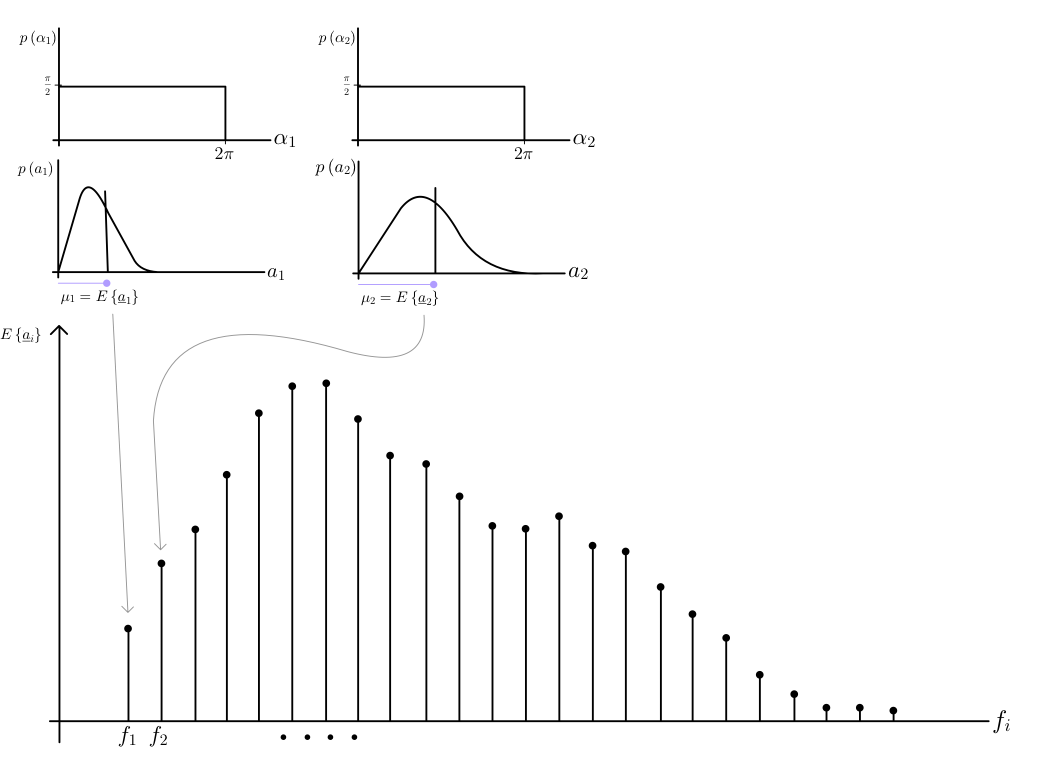
\includegraphics[width=.75\linewidth]{Figures/Theory/placeholder_randomModel.png}
    \caption{Visual explanation of the random phase/amplitude model. Every discrete frequency is represented by a uniform and Rayleigh distribution for the random phase and amplitude respectively. The top half of the figure depicts the random distributions at certain frequencies, and the bottom half depicts the amplitude spectrum as a function of frequency. Adapted from \cite{Holthuijsen2007}.}
    \label{fig:ap.randModel}
\end{figure}

\section{Energy Density Spectrum} \label{sec:sec:ap.oceanWaves.energySpectrum}
The energy density spectrum is more useful than the variance density spectrum as it shows the distribution of wave energy over various frequencies, where a narrower spectrum represents a more regular wave. The energy of a harmonic wave is given as the mean-square elevation times the gravitational acceleration, $g$, and the density of water, $\rho$. This gives the total energy as

\begin{equation} \label{eq:ap.waveSpectrum.totalEnergy}
   E_{total} = \rho g \overline{\underline{\eta}^{2}}
\end{equation}

Which allows the energy density spectrum to be obtained as

\begin{equation} \label{eq:ap.waveSpectrum.ESD}
   E_{energy}(f) = \rho g E_{variance}(f)
\end{equation}


%*****************************************************
%	APPENDIX
%*****************************************************
\chapter{\ac{hh} Technique Derivations}
\label{ap:hh}


This appendix contains mathematics derived by Hasselmann and Hasselmann \cite{Hasselmann1991} in 1991. This appendix serves as a summary of their paper and aims to present it in an easily understandable way.

\section{\ac{sar} Imaging of Ocean Waves} \label{ap:hh.sarImaging}

The surface elevation of a wave can be represented by the following equation.

\begin{equation}
    \eta(
\end{equation}


\section{Inversion Procedure} \label{ap:hh.inversion}

% Please add the following required packages to your document preamble:
% \usepackage[table,xcdraw]{xcolor}
% Beamer presentation requires \usepackage{colortbl} instead of \usepackage[table,xcdraw]{xcolor}
% \usepackage{longtable}
% Note: It may be necessary to compile the document several times to get a multi-page table to line up properly

%*****************************************************
%	APPENDIX
%*****************************************************
\chapter{\ac{s1a} Metadata Values}
\label{ap:metadata}
%% Update all links

Table \ref{tab:ap.metadataVals} shows all tabulated attribute names that can be used with the \href{https://github.com/JNSRYA006/sar-parameter-extraction-pipeline/blob/main/functions/preprocess/filterAttributesNetCDF.m}{\lstinline{filterAttributesNetCDF}} function. Additionally, Table \ref{tab:ap.metadataVals} is available as a \texttt{.csv} file on this project's \href{https://github.com/JNSRYA006/sar-parameter-extraction-pipeline/blob/main/functions/preprocess/filterAttributesNetCDF.m}{GitHub here}.

% Please add the following required packages to your document preamble:
% \usepackage[table,xcdraw]{xcolor}
% Beamer presentation requires \usepackage{colortbl} instead of \usepackage[table,xcdraw]{xcolor}
% \usepackage{longtable}
% Note: It may be necessary to compile the document several times to get a multi-page table to line up properly
% Please add the following required packages to your document preamble:
% \usepackage[table,xcdraw]{xcolor}
% Beamer presentation requires \usepackage{colortbl} instead of \usepackage[table,xcdraw]{xcolor}
% \usepackage{longtable}
% Note: It may be necessary to compile the document several times to get a multi-page table to line up properly
% Please add the following required packages to your document preamble:
% \usepackage[table,xcdraw]{xcolor}
% Beamer presentation requires \usepackage{colortbl} instead of \usepackage[table,xcdraw]{xcolor}
% \usepackage{longtable}
% Note: It may be necessary to compile the document several times to get a multi-page table to line up properly
\begin{longtable}[c]{|
>{\columncolor[HTML]{DADADA}}l |l|c|}
\hline
\cellcolor[HTML]{C0C0C0}\textbf{Attribute Name} & \cellcolor[HTML]{C0C0C0}\textbf{Description} & \cellcolor[HTML]{C0C0C0}\textbf{Unit} \\ \hline
\endfirsthead
%
\multicolumn{3}{c}%
{{\bfseries Table \thetable\ continued from previous page}} \\
\hline
\cellcolor[HTML]{C0C0C0}\textbf{Attribute Name} & \cellcolor[HTML]{C0C0C0}\textbf{Description} & \cellcolor[HTML]{C0C0C0}\textbf{Unit} \\ \hline
\endhead
%
PRODUCT & Product name &  \\ \hline
PRODUCT\_TYPE & Product type &  \\ \hline
SPH\_DESCRIPTOR & Description &  \\ \hline
MISSION & Satellite mission &  \\ \hline
ACQUISITION\_MODE & Acquisition mode &  \\ \hline
antenna\_pointing & Right or left facing &  \\ \hline
BEAMS & Beams used &  \\ \hline
SWATH & Swath name &  \\ \hline
PROC\_TIME & Processed time & utc \\ \hline
Processing\_system\_identifier & Processing system identified &  \\ \hline
orbit\_cycle & Cycle &  \\ \hline
REL\_ORBIT & Track &  \\ \hline
ABS\_ORBIT & Orbit &  \\ \hline
STATE\_VECTOR\_TIME & Time of orbit state vector & utc \\ \hline
VECTOR\_SOURCE & State vector source &  \\ \hline
incidence\_near &  & deg \\ \hline
incidence\_far &  & deg \\ \hline
slice\_num & Slice number &  \\ \hline
data\_take\_id & Data take  identifier &  \\ \hline
first\_line\_time & First zero doppler azimuth time & utc \\ \hline
last\_line\_time & Last zero doppler azimuth time & utc \\ \hline
first\_near\_lat &  & deg \\ \hline
first\_near\_long &  & deg \\ \hline
first\_far\_lat &  & deg \\ \hline
first\_far\_long &  & deg \\ \hline
last\_near\_lat &  & deg \\ \hline
last\_near\_long &  & deg \\ \hline
last\_far\_lat &  & deg \\ \hline
last\_far\_long &  & deg \\ \hline
PASS & ASCENDING or DESCENDING &  \\ \hline
SAMPLE\_TYPE & DETECTED or COMPLEX &  \\ \hline
mds1\_tx\_rx\_polar & Polarization &  \\ \hline
mds2\_tx\_rx\_polar & Polarization &  \\ \hline
mds3\_tx\_rx\_polar & Polarization &  \\ \hline
mds4\_tx\_rx\_polar & Polarization &  \\ \hline
polsar\_data & Polarimetric Matrix & flag \\ \hline
algorithm & Processing algorithm &  \\ \hline
azimuth\_looks &  &  \\ \hline
range\_looks &  &  \\ \hline
range\_spacing & Range sample spacing & m \\ \hline
azimuth\_spacing & Azimuth sample spacing & m \\ \hline
range\_window\_type & Range window type &  \\ \hline
range\_window\_coefficient & Range window coefficient &  \\ \hline
pulse\_repetition\_frequency & PRF & Hz \\ \hline
radar\_frequency & Radar frequency & MHz \\ \hline
line\_time\_interval &  & s \\ \hline
total\_size & Total product size & MB \\ \hline
num\_output\_lines & Raster height & lines \\ \hline
num\_samples\_per\_line & Raster width & samples \\ \hline
subset\_offset\_x & \begin{tabular}[c]{@{}l@{}}X coordinate of UL corner of subset\\ in original image\end{tabular} & samples \\ \hline
subset\_offset\_y & \begin{tabular}[c]{@{}l@{}}Y coordinate of UL corner of subset\\ in original image\end{tabular} & samples \\ \hline
srgr\_flag & SRGR applied & flag \\ \hline
avg\_scene\_height & Average scene height ellipsoid & m \\ \hline
map\_projection & Map projection applied & flag \\ \hline
is\_terrain\_corrected & Orthorectification applied & flag \\ \hline
DEM & Digital Elevation Model used &  \\ \hline
geo\_ref\_system & Geographic reference system &  \\ \hline
lat\_pixel\_res & Pixel resolution in geocoded image & deg \\ \hline
lon\_pixel\_res & Pixel resolution in geocoded image & deg \\ \hline
slant\_range\_to\_first\_pixel & Slant range to 1st data sample & m \\ \hline
ant\_elev\_corr\_flag & Antenna elevation applied & flag \\ \hline
range\_spread\_comp\_flag & Range spread compensation applied & flag \\ \hline
replica\_power\_corr\_flag & Replica pulse power correction applied & flag \\ \hline
abs\_calibration\_flag & Product calibrated & flag \\ \hline
calibration\_factor & Calibration constant & dB \\ \hline
chirp\_power & Chirp power &  \\ \hline
inc\_angle\_comp\_flag & Incidence angle compensation applied & flag \\ \hline
ref\_inc\_angle & Reference incidence angle &  \\ \hline
ref\_slant\_range & Reference slant range &  \\ \hline
ref\_slant\_range\_exp & Reference slant range exponent &  \\ \hline
rescaling\_factor & Rescaling factor & flag \\ \hline
bistatic\_correction\_applied &  & flag \\ \hline
range\_sampling\_rate & Range sampling rate & MHz \\ \hline
range\_bandwidth & Bandwidth total in range & MHz \\ \hline
azimuth\_bandwidth & Bandwidth total in azimuth & Hz \\ \hline
multilook\_flag & Multilook applied & flag \\ \hline
coregistered\_stack & Coregistration applied & flag \\ \hline
external\_calibration\_file & External calibration file used &  \\ \hline
orbit\_state\_vector\_file & Orbit file used &  \\ \hline
metadata\_version & AbsMetadata version &  \\ \hline
centre\_lat &  & deg \\ \hline
centre\_lon &  & deg \\ \hline
centre\_heading &  & deg \\ \hline
centre\_heading2 &  & deg \\ \hline
Orbit\_State\_Vectors:orbit\_vectorx:time & Time of x number orbit state vector & utc \\ \hline
Orbit\_State\_Vectors:orbit\_vectorx:x\footnote{x here denotes the number of the orbit vector to request metadata for.}\_pos & x position of x number orbit state vector & m \\ \hline
Orbit\_State\_Vectors:orbit\_vectorx:y\_pos & y position of x number orbit state vector & m \\ \hline
Orbit\_State\_Vectors:orbit\_vectorx:z\_pos & z position of x number orbit state vector & m \\ \hline
Orbit\_State\_Vectors:orbit\_vectorx:x\_vel & x velocity of x number orbit state vector & m/s \\ \hline
Orbit\_State\_Vectors:orbit\_vectorx:y\_vel & y velocity of x number orbit state vector & m/s \\ \hline
Orbit\_State\_Vectors:orbit\_vectorx:z\_vel & z velocity of x number orbit state vector & m/s \\ \hline
Band\_xx\footnote{xx here denotes the capture mode of \acs{s1a} data. Examples include \acs{iw} or \acs{ew}. More detail on \acs{s1a} capture modes can be found in Section \ref{subsec:theory.sar.imaging}.}\_yy\footnote{yy here denotes the polarisation of \acs{s1a} data. Examples include VV or VH. More detail on \acs{s1a} polarisation can be found in Section \ref{subsec:theory.sar.polarisation}.}:swath & Swath name &  \\ \hline
Band\_xx\_yy:polarization & Polarization &  \\ \hline
Band\_xx\_yy:annotation & metadata file &  \\ \hline
Band\_xx\_yy:band\_names & corresponding bands &  \\ \hline
Band\_xx\_yy:first\_line\_time & First zero doppler azimuth time & utc \\ \hline
Band\_xx\_yy:last\_line\_time & Last zero doppler azimuth time & utc \\ \hline
Band\_xx\_yy:line\_time\_interval & Time per line & s \\ \hline
Band\_xx\_yy:num\_output\_lines & Raster height & lines \\ \hline
Band\_xx\_yy:num\_samples\_per\_line & Raster width & samples \\ \hline
Band\_xx\_yy:sample\_type & DETECTED or COMPLEX &  \\ \hline
Band\_xx\_yy:calibration\_factor & Calibration constant &  \\ \hline
\caption{\acs{s1a} \acs{netcdf} exported metadata values. Attribute Names given can be used with filterAtt function.}
\label{tab:ap.metadataVals}\\
\end{longtable}
%*****************************************************
%	APPENDIX
%*****************************************************
\chapter{MATLAB Live Script}
\label{ap:liveScript}

This appendix contains a copy of the unrun \href{https://github.com/JNSRYA006/sar-parameter-extraction-pipeline/blob/main/functions/pipeline.mlx}{\lstinline{pipeline.mlx}} script which is classed as the pipeline for this project.

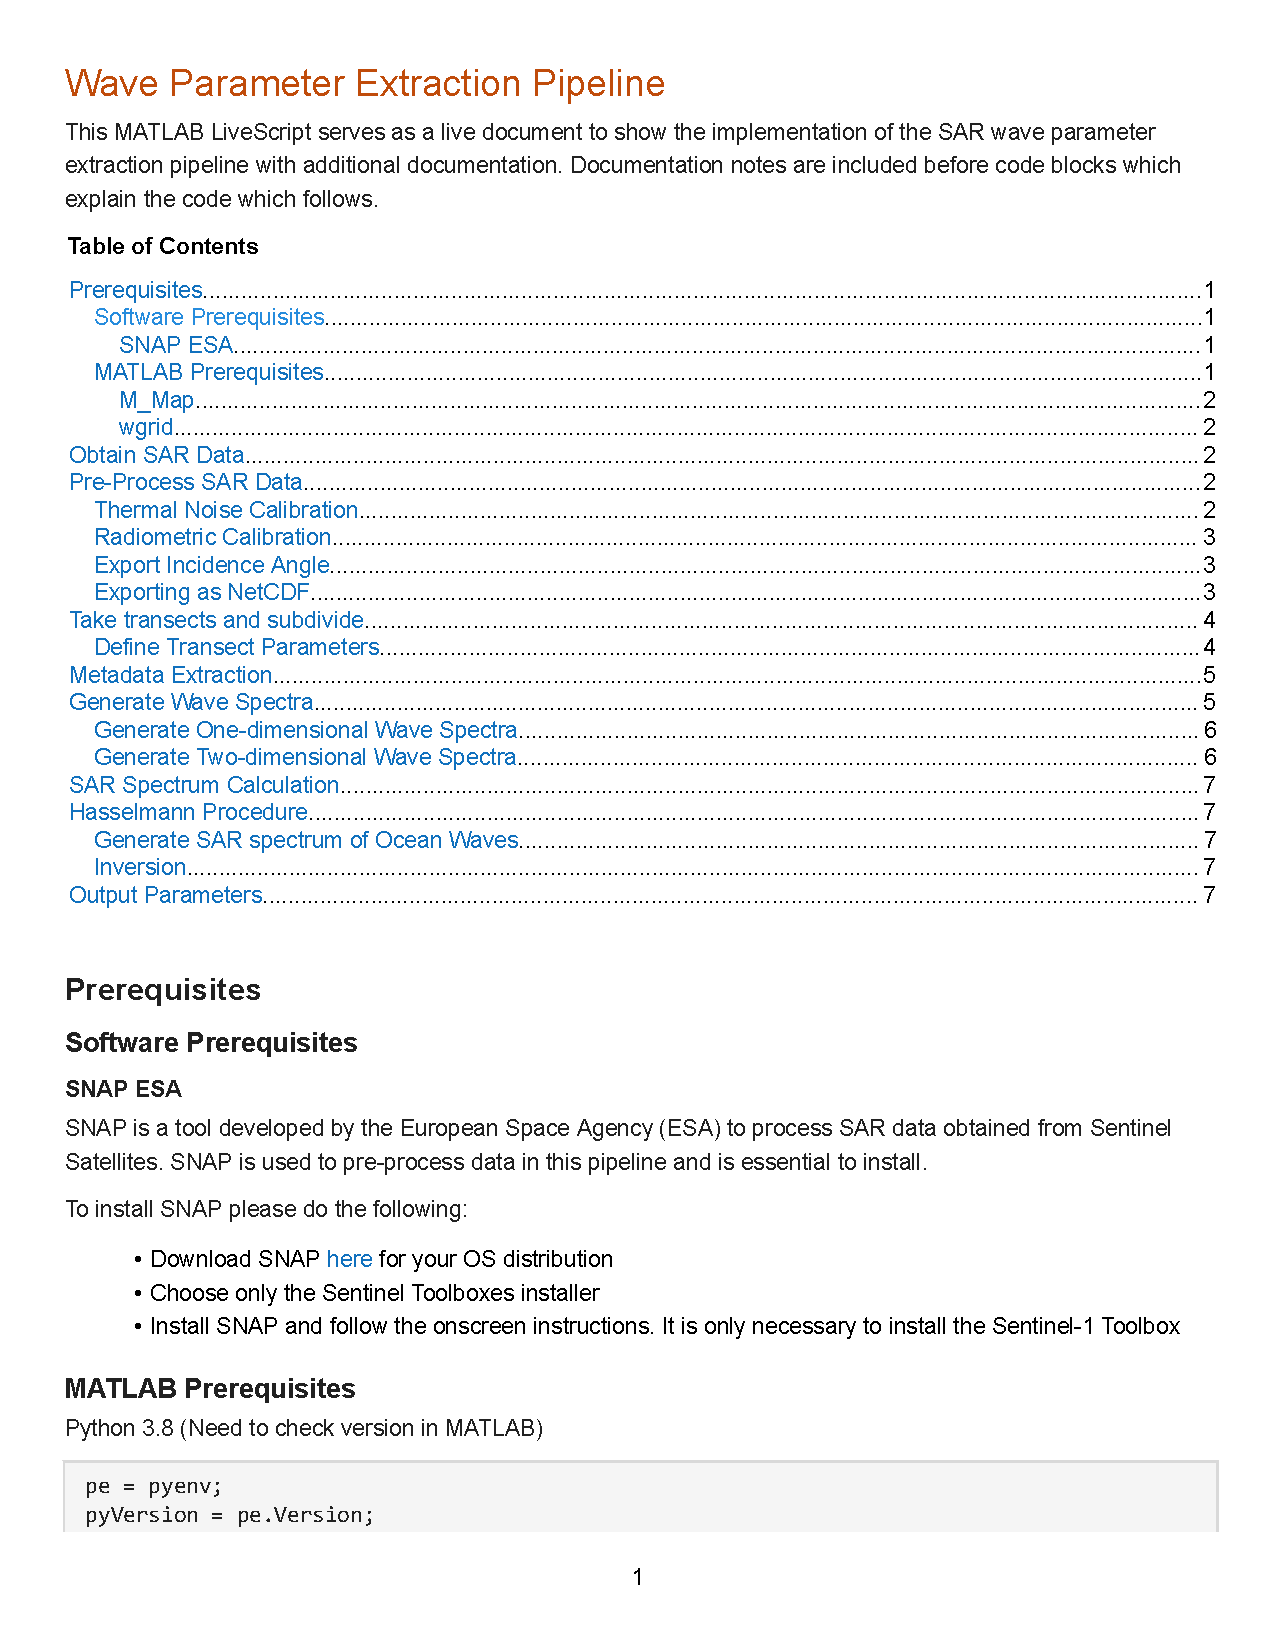
\includepdf[pages=-]{Figures/Appendices/pipeline.pdf}

% \begin{figure}[htp] \centering{
% 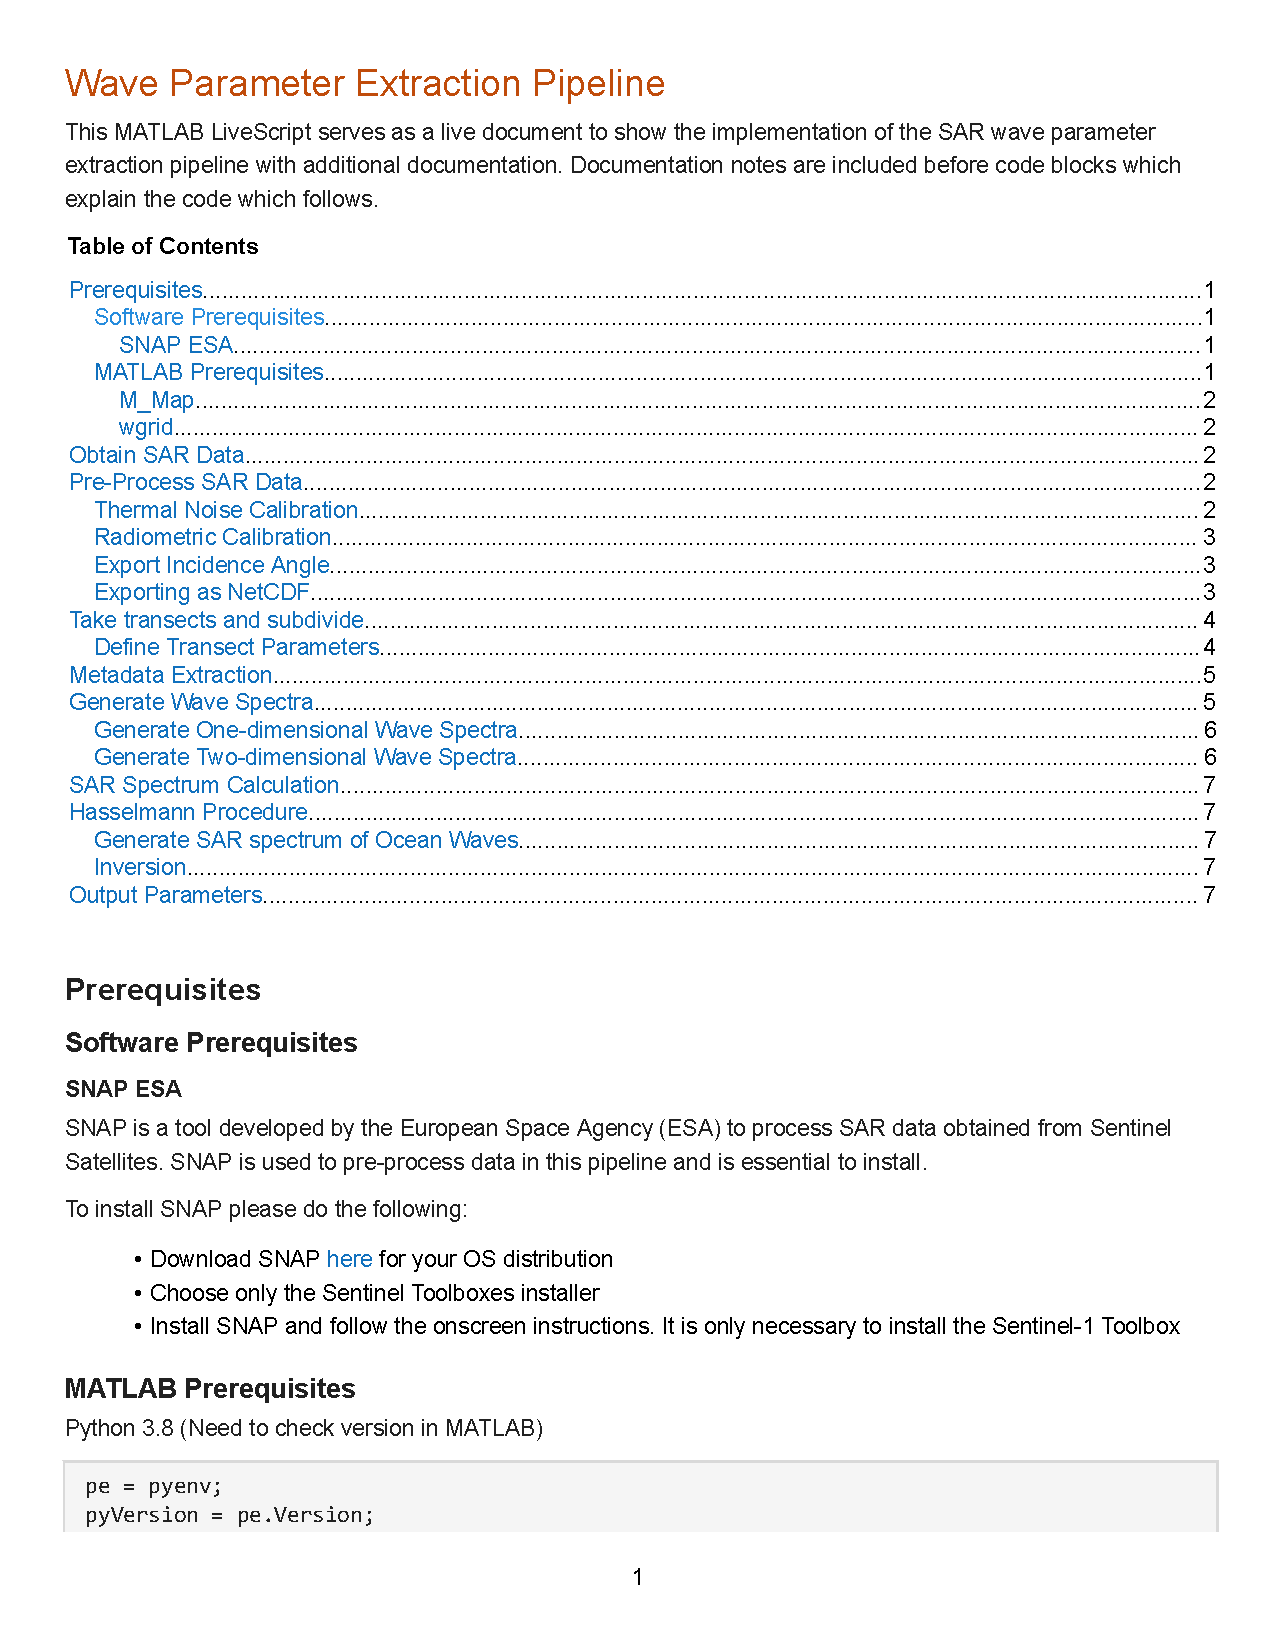
\includegraphics[scale=0.7]{Figures/Appendices/pipeline.pdf}}
% \caption{Full, unrun pipeline. This \textsc{Matlab} script is available on \href{https://github.com/JNSRYA006/sar-parameter-extraction-pipeline/blob/main/functions/pipeline.mlx}{GitHub}.}
% \label{fig:ap.pipeline}
% \end{figure}  

% \begin{figure}[H]
%     \centering
%     \resizebox{0.95\linewidth}{!}{% This LaTeX was auto-generated from MATLAB code.
% To make changes, update the MATLAB code and export to LaTeX again.

\sloppy
\epstopdfsetup{outdir=./}
\graphicspath{ {./pipeline_images/} }

\matlabhastoc


\label{T_B8033DED}
\matlabtitle{Wave Parameter Extraction Pipeline}

\begin{par}
\begin{flushleft}
This MATLAB LiveScript serves as a live document to show the implementation of the SAR wave parameter extraction pipeline with additional documentation. Documentation notes are included before code blocks which explain the code which follows.
\end{flushleft}
\end{par}

\matlabtableofcontents{Table of Contents}

\label{H_45278BA7}
\matlabheading{Prerequisites}

\label{H_603A9976}
\matlabheadingtwo{Software Prerequisites}

\label{H_FF806E53}
\matlabheadingthree{SNAP ESA}

\begin{par}
\begin{flushleft}
SNAP is a tool developed by the European Space Agency (ESA) to process SAR data obtained from Sentinel Satellites. SNAP is used to pre-process data in this pipeline and is essential to install.
\end{flushleft}
\end{par}

\begin{par}
\begin{flushleft}
To install SNAP please do the following:
\end{flushleft}
\end{par}

\begin{itemize}
\setlength{\itemsep}{-1ex}
   \item{\begin{flushleft} Download SNAP \href{https://step.esa.int/main/download/snap-download/}{here} for your OS distribution \end{flushleft}}
   \item{\begin{flushleft} Choose only the Sentinel Toolboxes installer \end{flushleft}}
   \item{\begin{flushleft} Install SNAP and follow the onscreen instructions. It is only necessary to install the Sentinel-1 Toolbox \end{flushleft}}
\end{itemize}

\label{H_69BBBAC5}
\matlabheadingtwo{MATLAB Prerequisites}

\begin{par}
\begin{flushleft}
Python 3.8 (Need to check version in MATLAB)
\end{flushleft}
\end{par}

\begin{matlabcode}
pe = pyenv;
pyVersion = pe.Version;
if ~(strcmp(pyVersion, "3.8"))
    pe(Version="3.8")
end
\end{matlabcode}

\begin{par}
\begin{flushleft}
CDS Toolbox
\end{flushleft}
\end{par}

\label{H_E263194C}
\matlabheadingthree{M\_Map}

\begin{par}
\begin{flushleft}
M\_Map is a mapping package for MATLAB which allows data plots on different world maps.
\end{flushleft}
\end{par}

\begin{par}
\begin{flushleft}
To use M\_Map please do the following:
\end{flushleft}
\end{par}

\begin{itemize}
\setlength{\itemsep}{-1ex}
   \item{\begin{flushleft} Download the zipped package \href{https://www.eoas.ubc.ca/~rich/map.html#download}{here} and \end{flushleft}}
   \item{\begin{flushleft} Add the extracted folder to your MATLAB path \end{flushleft}}
\end{itemize}

\begin{par}
\begin{flushleft}
\textit{Note:} A copy of the M\_Map package is included on this git repo in the following path: 
\end{flushleft}
\end{par}

\label{H_ADB0A04B}
\matlabheadingthree{wgrid}


\label{H_7B094A5D}
\matlabheading{Obtain SAR Data}

\begin{par}
\begin{flushleft}
SAR data from Sentinel-1A can be downloaded from \href{https://scihub.copernicus.eu/dhus/#/home}{Copernicus SciHub}. In order to download data, you need to register an account on the site.
\end{flushleft}
\end{par}

\begin{par}
\begin{flushleft}
Once you have registered your account, you can search for SAR data on the site by choosing the appropriate filters and region. The region you search is set by right-clicking and drawing a rectangle, otherwise you can left-click and draw the vertices of any polygon. Recomended filters are:
\end{flushleft}
\end{par}

\begin{enumerate}
\setlength{\itemsep}{-1ex}
   \item{\begin{flushleft} \textbf{Sensing Period: }As desired \end{flushleft}}
   \item{\begin{flushleft} \textbf{Satellite Platform:} S1A \end{flushleft}}
   \item{\begin{flushleft} \textbf{Product Type:} GRD \end{flushleft}}
   \item{\begin{flushleft} \textbf{Polarisation:} As desired \end{flushleft}}
\end{enumerate}

\begin{par}
\begin{flushleft}
After searching with your filters, you will see all the available data within this region. Clicking on a red footprint on the map, shows a preview of these data, and the data can be downloaded from the pop-up. 
\end{flushleft}
\end{par}

\begin{par}
\begin{flushleft}
\textit{Note: }These data are in excess of 1GB, so large amounts of storage space is required. Use an external hard drive if possible.
\end{flushleft}
\end{par}


\label{H_1D14B3F6}
\matlabheading{\textbf{Pre-Process SAR Data}}

\begin{par}
\begin{flushleft}
After downloading SAR data from \href{https://scihub.copernicus.eu/dhus/#/home}{Copernicus SciHub}, open \hyperref[H_FF806E53]{SNAP} and import the data. These data can be viewed as follows:
\end{flushleft}
\end{par}

\begin{enumerate}
\setlength{\itemsep}{-1ex}
   \item{\begin{flushleft} Click the '+' next to the dataset \end{flushleft}}
   \item{\begin{flushleft} Click the '+' next to the \textit{Bands} folder \end{flushleft}}
   \item{\begin{flushleft} Open the desired band to preview the image \end{flushleft}}
\end{enumerate}

\label{H_B7EBD40C}
\matlabheadingtwo{Thermal Noise Calibration}

\begin{par}
\begin{flushleft}
\textbf{This needs to be done first}
\end{flushleft}
\end{par}

\begin{par}
\begin{flushleft}
To remove thermal noise, click \textit{Radar -\textgreater{} Radiometric -\textgreater{} S1 Thermal Noise Removal. }This will bring up a window where the following needs to be done.
\end{flushleft}
\end{par}

\begin{enumerate}
\setlength{\itemsep}{-1ex}
   \item{\begin{flushleft} Ensure the file will save as \textit{BEAM-DIMAP} \end{flushleft}}
   \item{\begin{flushleft} Check that \textit{Remove Thermal Noise} is checked in the \textit{Processing Parameters} window \end{flushleft}}
   \item{\begin{flushleft} Select a specific polarisation (If desired) \end{flushleft}}
   \item{\begin{flushleft} Rename the output file (\textit{Target Product) }if desired \end{flushleft}}
   \item{\begin{flushleft} Check the \textit{Open in SNAP} checkbox \end{flushleft}}
\end{enumerate}

\begin{par}
\begin{flushleft}
After clicking \textit{Run,} SNAP will begin removing thermal noise from the selected data and once complete will open in the \textit{Product Explorer }sidebar.
\end{flushleft}
\end{par}

\label{H_0477ED49}
\matlabheadingtwo{Radiometric Calibration}

\begin{par}
\begin{flushleft}
To radiometrically calibrate the SAR data, ensure that the \textbf{noise calibrated product is selected}, then click \textit{Radar -\textgreater{} Radiometric -\textgreater{} Calibrate }This will bring up a window where the following needs to be done.
\end{flushleft}
\end{par}

\begin{enumerate}
\setlength{\itemsep}{-1ex}
   \item{\begin{flushleft} Ensure the file will save as \textit{BEAM-DIMAP} \end{flushleft}}
   \item{\begin{flushleft} Check that \textbf{only} \textit{Output sigma0 band} is checked in the \textit{Processing Parameters} window \end{flushleft}}
   \item{\begin{flushleft} Select a specific polarisation (If desired) \end{flushleft}}
   \item{\begin{flushleft} Rename the output file (\textit{Target Product) }if desired \end{flushleft}}
   \item{\begin{flushleft} Check the \textit{Open in SNAP} checkbox \end{flushleft}}
\end{enumerate}

\begin{par}
\begin{flushleft}
After clicking \textit{Run,} SNAP will begin radiometric calibration from the selected data and once complete will open in the \textit{Product Explorer }sidebar.
\end{flushleft}
\end{par}

\label{H_C1EC94A9}
\matlabheadingtwo{Export Incidence Angle}

\begin{par}
\begin{flushleft}
In order to access the incidence angle of each pixel in the the SAR data, the following process needs to be followed.
\end{flushleft}
\end{par}

\begin{enumerate}
\setlength{\itemsep}{-1ex}
   \item{\begin{flushleft} Click the '+' next to the \textit{Tie-Point Grids} folder \end{flushleft}}
   \item{\begin{flushleft} Right-click on the \textit{incident\_angle} band \end{flushleft}}
   \item{\begin{flushleft} Select \textit{Band Maths} \end{flushleft}}
   \item{\begin{flushleft} Rename the band to "Incidence\_Angle" and click OK \end{flushleft}}
\end{enumerate}

\label{H_69B1A933}
\matlabheadingtwo{Exporting as NetCDF}

\begin{par}
\begin{flushleft}
In order to export these pre-processed SAR data in a format supported by MATLAB, the following process needs to be followed.
\end{flushleft}
\end{par}

\begin{enumerate}
\setlength{\itemsep}{-1ex}
   \item{\begin{flushleft} Click \textit{File} \end{flushleft}}
   \item{\begin{flushleft} Hover over the \textit{Export} option, and select \textbf{NetCDF4-BEAM} \end{flushleft}}
   \item{\begin{flushleft} If your file explorer is opened, click on \textit{Subset... }on the right hand side of the dialog box \end{flushleft}}
   \item{\begin{flushleft} This will bring up a new window with four different menus. \end{flushleft}}
   \item{\begin{flushleft} You can take a Spatial Subset of the image using either pixel or geographical coordinates in the \textit{Spatial Subset }menu \end{flushleft}}
   \item{\begin{flushleft} Ensure that under the \textit{Band Subset} menu, your desired bands are selected, as well as your created \textit{\textbf{Incidence\_Angle}}\textbf{ band. } \end{flushleft}}
   \item{\begin{flushleft} Ensure that under the \textit{Metadata Subset} menu, all options are selected \end{flushleft}}
   \item{\begin{flushleft} After checking all of these parameters, click OK, and name the file as desired and save it in your desired location \end{flushleft}}
\end{enumerate}

\begin{par}
\begin{flushleft}
Optional
\end{flushleft}
\end{par}


\vspace{1em}

\label{H_A008662F}
\matlabheading{Take transects and subdivide}

\begin{par}
\begin{flushleft}
After exporting the SAR data as a NetCDF file, use the following commands to import the data and metadata into MATLAB.
\end{flushleft}
\end{par}

\begin{matlabcode}
filepath = "D:\UCT\EEE4022S\Data\CPT\smaller_subset_incidence.nc";
% Import data values
ncImport = ncinfo(filepath);
% Update the band to import as required
sarData = ncread(filepath,'Sigma0_VV');
metadata = ncinfo(filepath,'metadata');
incidenceAngle = ncread(filepath,'Incidence_Angle');
\end{matlabcode}


\label{H_82C18072}
\matlabheadingtwo{Define Transect Parameters}

\begin{par}
\begin{flushleft}
Enter the number of desired transects to take, the start point (in pixels), along with the angle at which to take the transects. This angle is calculated from the positive x-axis clockwise.
\end{flushleft}
\end{par}

\begin{matlabcode}
% Enter the number of transects
n = 3;
th = 10;
[transectData, positions] = get512Transects(sarData,1,1,th,n);
\end{matlabcode}

\begin{par}
\begin{flushleft}
The original data, with shown transects can be plotted as follows.
\end{flushleft}
\end{par}

\begin{matlabcode}
figure(1)
imshow(sarData)
hold on;

for i = 1:n
    annotate512Transect(positions(i,1),positions(i,2),i,'red','black',1);
end

title('Sentinel-1A data with transects displayed')
hold off
\end{matlabcode}

\begin{par}
\begin{flushleft}
The individual transects can be plotted as follows.
\end{flushleft}
\end{par}

\begin{matlabcode}
figure(2)
subplot(1,3,1)
imshow(transectData(:,:,1));
title(['Transect 1 at ',num2str(th),' degrees'])
subplot(1,3,2)
imshow(transectData(:,:,2));
title(['Transect 2 at ',num2str(th),' degrees'])
subplot(1,3,3)
imshow(transectData(:,:,3));
title(['Transect 3 at ',num2str(th),' degrees'])
\end{matlabcode}

\begin{par}
\begin{flushleft}
Metadata can be imported using the \texttt{ncinfo} function. This large metadata structure can be slimmed down by filtering using the desired attributes for subsequent functions.
\end{flushleft}
\end{par}

\begin{matlabcode}
% Metadata
%metadata = ncinfo(filepath,'metadata');
req_atributes = ["first_near_lat","first_near_long","first_far_lat","first_far_long","last_near_lat","last_near_long","last_far_lat","last_far_long","centre_lat","centre_lon", "num_output_lines","num_samples_per_line"];
metadata_filtered = filterAttributesNetCDF(metadata.Attributes, req_atributes);
\end{matlabcode}


\label{H_1A16A1DF}
\matlabheading{Metadata Extraction}


\vspace{1em}

\vspace{1em}

\label{H_357F0BDA}
\matlabheading{Generate Wave Spectra}

\begin{par}
\begin{flushleft}
Before generating wave spectra, please source data from \href{https://nomads.ncep.noaa.gov/pub/data/nccf/com/gfs/prod/}{NOAA NCEP here}. Ensure that you select data in the following manner.
\end{flushleft}
\end{par}

\begin{enumerate}
\setlength{\itemsep}{-1ex}
   \item{\begin{flushleft} Select data of the following form: \texttt{\textbf{gdas.date}} \end{flushleft}}
   \item{\begin{flushleft} Select the desired time (Either \texttt{00/}, \texttt{06/}, \texttt{12/}, or \texttt{18/}) \end{flushleft}}
   \item{\begin{flushleft} Select \texttt{wave/} data \end{flushleft}}
   \item{\begin{flushleft} Choose the \texttt{gridded/ }data \end{flushleft}}
   \item{\begin{flushleft} Once completing all of the above, choose any data in the following form: \texttt{gdaswave.}\texttt{\textbf{time}}\texttt{z.}\texttt{\textbf{location}}\texttt{.0p25.f000.grib2, }where the \textbf{bold} values are user decided variables \end{flushleft}}
   \item{\begin{flushleft} After choosing a data set, right-click and copy the link address \end{flushleft}}
\end{enumerate}

\begin{par}
\begin{flushleft}
Parse in your chosen dataset
\end{flushleft}
\end{par}

\begin{matlabcode}
noaaUrl = "https://nomads.ncep.noaa.gov/pub/data/nccf/com/gfs/prod/gdas.20231002/12/wave/gridded/gdaswave.t12z.gsouth.0p25.f000.grib2";
\end{matlabcode}

\begin{par}
\begin{flushleft}
Set the name for the saved downloaded \texttt{.grib2} file and the file will be downloaded and saved.
\end{flushleft}
\end{par}

\begin{matlabcode}
waveDownloadName = "wave_data.grib2";
waveFilePath = downloadNOAAWaveFile(noaaUrl,waveDownloadName);
\end{matlabcode}

\begin{par}
\begin{flushleft}
Set the location of wgib and the downloaded \texttt{.grib2} filepath as well as choosing if you'd like to plot your downloaded data along with the type to plot
\end{flushleft}
\end{par}

\begin{matlabcode}
GribPath = "C:\Users\ryanj\OneDrive - University of Cape Town\4. Fourth Year\Second Semester\EEE4022S\repo\sar-parameter-extraction-pipeline\functions\";
wgrib2Path = "C:\Users\ryanj\Downloads";
waveStruct = getGribStruct(wgrib2Path,GribPath);
noaaPlot = true;
noaaValToPlot = 'direction';
if noaaPlot
    noaaDataPlot('miller',waveStruct,noaaValToPlot);
end
\end{matlabcode}

\begin{par}
\begin{flushleft}
Set the location at which to generate wave spectra for
\end{flushleft}
\end{par}

\begin{matlabcode}
latitude = -34.2;
longitude = 18.6;
[gridLat, gridLon] = createLatLonGrid(latitude, longitude, resolution);
startLat = max(gridLat)
startLon = min(gridLon)
endLat = min(gridLat)
endLon = max(gridLon)
waveVals = getSubsetWaveVals(waveStruct,startLat,startLon,endLat,endLon);
\end{matlabcode}

\label{H_D6296C3F}
\matlabheadingtwo{Generate One-dimensional Wave Spectra}

\begin{par}
\begin{flushleft}
Define and instantiate variables for the one-dimensional wave spectra
\end{flushleft}
\end{par}

\begin{matlabcode}
imageSize = size(sarData,1);
w = linspace(0,2*pi,imageSize)';
f = linspace(0,1,imageSize)';
Hs = waveVals.significantWaveHeight(1,1);
T0 = waveVals.significantWavePeriod(1,1);
w0 = 2*pi./T0;
f0 = 1./T0;
gammaVal = 1.308;
multipleWaveSpectra = false;
if multipleWaveSpectra
    S = generateMultipleJONSWAP(waveVals,gammaVal,w,1);   
else
    S = generateSingleJONSWAP(Hs,w0,gammaVal,w);
end
\end{matlabcode}

\label{H_D690D0F0}
\matlabheadingtwo{Generate Two-dimensional Wave Spectra}

\begin{matlabcode}
[D,theta] = generateDirectionalDistribution(waveVals,w,1);
E = generate2DWaveSpectrum(S,D);
\end{matlabcode}


\vspace{1em}

\label{H_63792B58}
\matlabheading{SAR Spectrum Calculation}


\vspace{1em}

\label{H_B1CC5E95}
\matlabheading{Hasselmann Procedure}


\vspace{1em}

\vspace{1em}
\label{H_893CF502}
\matlabheadingtwo{Generate SAR spectrum of Ocean Waves}


\vspace{1em}
\label{H_F29E6812}
\matlabheadingtwo{Inversion}


\vspace{1em}

\label{H_06FC8CFF}
\matlabheading{Output Parameters}
}
%     \caption{}
%     \label{fig:ap.pipeline}
% \end{figure}

%=====================================================================
%	BACK MATTER
%=====================================================================

\backmatter

%---------------------------------------------------------------------
%	BIBLIOGRAPHY
%---------------------------------------------------------------------

\bibliographystyle{IEEEtran}
\bibliography{report}

%---------------------------------------------------------------------
\end{document}
%---------------------------------------------------------------------
%	End of the document
%=====================================================================
